% Short demo for \LaTeX beamer theme with ACON style layout
%
% Author: Thomas Meurer <tm@tf.uni-kiel.de>
% Version history:
% v0 ... 2016/12/09

\documentclass[10pt,t,aspectratio=1610]{beamer}
%\usetheme[german]{ACON} %or 
\usetheme{ACON}

% We define  a command \sfcite which enables to add citations but to
% preserve the citation number throughout the presentation. Citations
% are placed on the slide, where \sfcite is called. For the standard
% behavior of citations use \footcite.
%
% This also requires to add the following two lines to the main LaTeX
% source file:
%
\usepackage[style=numeric-comp,citetracker=true,sorting=none]{biblatex}
\bibliography{example}
\usepackage{abbreviations} %Provide an abbreviations file if equations
                          %are used
\usepackage{curve2e}

% -----------------------
% By JW
\usepackage{subfigure}
\usepackage{tabularx}
\usepackage{multicol}
\usepackage{xcolor}

\usepackage{pgf} % For .pgf Plot-Saves

\usepackage{wrapfig}

\usepackage{hyperref}

\definecolor{light-gray}{gray}{0.95}
\newcommand{\code}[1]{\colorbox{light-gray}{\texttt{#1}}}
% -----------------------

% =======================

% If the title exceeds two lines then adjust the title font size 
%\setbeamerfont{title}{series=\bfseries,size={\fontsize{18}{18}}}

% =======================

\title{Eine Anwendung des Reinforcement Learning zur Regelung dynamischer Systeme}
\subtitle{Status zum 18. Juli 2018}
\author[J. Wilinski]{Jonas Helmut Wilinski}
\pauthoremail{stu118261@mail.uni-kiel.de}
\institute[ACON]{Statusgespräch}
\date{Mittwoch, 18. Juli 2018}
\begin{document}

% =======================

\begin{frame}[plain]
  \titlepage
\end{frame}

% =======================

\begin{frame}
  \frametitle{Bisherige Schritte}
  \framesubtitle{Literaturphase}

  \begin{itemize}
  \item Mehrere Paper \& Fachliteratur gelesen und zusammengefasst
    \begin{itemize}
    \item \btEmph{Bücher}
    	\begin{itemize}
    		\item Stuart Russell, Peter Norvig - Artificial Intelligence - A Modern Approach (2010, Prentice Hall)
    		\item Raúl Rojas (auth.) - Theorie der neuronalen Netze - Eine systematische Einführung (1993, Springer-Verlag Berlin Heidelberg)
    		\item Steven H. Strogatz - Nonlinear Dynamics and Chaos - With Applications to Physics, Biology, Chemistry, and Engineering  (1994, Westview Press)
    		\item \textbf{Wulfram Gerstner, Werner M. Kistler, Richard Naud, Liam Paninski - Neuronal Dynamics - From Single Neurons to Networks and Models of Cognition (2014, Cambridge University Press)
    		}
    	\end{itemize}
    \item \btEmph{Fachartikel}
    	\begin{itemize}
    		\item Lechner (et al) - Worm-level control through search-based reinforcement learning
    		\item Lechner (et al) - Neuronal Circuit Policies
    		\item SIM-CE - An advanced Simulink platform for studying the brain of C. elegans
    	\end{itemize}
    \item \btEmph{Kurse}
    	\begin{itemize}
    		\item Reinforcement Learning by David Silver (Google DeepMind – UCL)
    	\end{itemize}
    \end{itemize}
  \end{itemize}  
\end{frame}

% =======================

\begin{frame}[fragile]
  \frametitle{Bisherige Schritte}
  \framesubtitle{Implementierung des \btEmph{Leaky Integrate and Fire - Modells}}

  \begin{itemize}
  	\item Programmiersprache \code{Python}
  	\begin{itemize}
  		\item Stuart Russell, Peter Norvig - Artificial Intelligence - A Modern Approach (2010, Prentice Hall)
  		\item Raúl Rojas (auth.) - Theorie der neuronalen Netze - Eine systematische Einführung (1993, Springer-Verlag Berlin Heidelberg)
  		\item Steven H. Strogatz - Nonlinear Dynamics and Chaos - With Applications to Physics, Biology, Chemistry, and Engineering  (1994, Westview Press)
  		\item \textbf{Wulfram Gerstner, Werner M. Kistler, Richard Naud, Liam Paninski - Neuronal Dynamics - From Single Neurons to Networks and Models of Cognition (2014, Cambridge University Press)
  		}
  	\end{itemize}
  	\item Zusätzliche Libraries
  	\begin{itemize}
  		\item Mathematische Berechnungen \& Matrizen durch die Python-Library \code{NumPy}
  		\item Darstellung durch die Python-Library \code{Matplotlib}
  	\end{itemize}
  	\item Leaky Integrate and Fire - Modell
  	\begin{itemize}
  		\item Lösung der Differentialgleichung durch nummerische Verfahren:
  		  \begin{itemize}
  		  	\item Euler-Verfahren
  		  	\item \textbf{Runge-Kutta 2. \& 4. Ordnung}
  		  \end{itemize}
  	\end{itemize}
  \end{itemize}
	

\end{frame}

% =======================

\begin{frame}
	\frametitle{Bisherige Schritte}
	\framesubtitle{Plot des LIF-Modells}
	
	\begin{center}
	  \scalebox{0.2}{%% Creator: Matplotlib, PGF backend
%%
%% To include the figure in your LaTeX document, write
%%   \input{<filename>.pgf}
%%
%% Make sure the required packages are loaded in your preamble
%%   \usepackage{pgf}
%%
%% Figures using additional raster images can only be included by \input if
%% they are in the same directory as the main LaTeX file. For loading figures
%% from other directories you can use the `import` package
%%   \usepackage{import}
%% and then include the figures with
%%   \import{<path to file>}{<filename>.pgf}
%%
%% Matplotlib used the following preamble
%%   \usepackage{fontspec}
%%   \setmainfont{Times New Roman}
%%   \setsansfont{Verdana}
%%   \setmonofont{Courier New}
%%
\begingroup%
\makeatletter%
\begin{pgfpicture}%
\pgfpathrectangle{\pgfpointorigin}{\pgfqpoint{15.360000in}{7.670000in}}%
\pgfusepath{use as bounding box, clip}%
\begin{pgfscope}%
\pgfsetbuttcap%
\pgfsetmiterjoin%
\definecolor{currentfill}{rgb}{1.000000,1.000000,1.000000}%
\pgfsetfillcolor{currentfill}%
\pgfsetlinewidth{0.000000pt}%
\definecolor{currentstroke}{rgb}{1.000000,1.000000,1.000000}%
\pgfsetstrokecolor{currentstroke}%
\pgfsetdash{}{0pt}%
\pgfpathmoveto{\pgfqpoint{0.000000in}{0.000000in}}%
\pgfpathlineto{\pgfqpoint{15.360000in}{0.000000in}}%
\pgfpathlineto{\pgfqpoint{15.360000in}{7.670000in}}%
\pgfpathlineto{\pgfqpoint{0.000000in}{7.670000in}}%
\pgfpathclose%
\pgfusepath{fill}%
\end{pgfscope}%
\begin{pgfscope}%
\pgfsetbuttcap%
\pgfsetmiterjoin%
\definecolor{currentfill}{rgb}{1.000000,1.000000,1.000000}%
\pgfsetfillcolor{currentfill}%
\pgfsetlinewidth{0.000000pt}%
\definecolor{currentstroke}{rgb}{0.000000,0.000000,0.000000}%
\pgfsetstrokecolor{currentstroke}%
\pgfsetstrokeopacity{0.000000}%
\pgfsetdash{}{0pt}%
\pgfpathmoveto{\pgfqpoint{1.920000in}{0.843700in}}%
\pgfpathlineto{\pgfqpoint{13.824000in}{0.843700in}}%
\pgfpathlineto{\pgfqpoint{13.824000in}{6.749600in}}%
\pgfpathlineto{\pgfqpoint{1.920000in}{6.749600in}}%
\pgfpathclose%
\pgfusepath{fill}%
\end{pgfscope}%
\begin{pgfscope}%
\pgfsetbuttcap%
\pgfsetroundjoin%
\definecolor{currentfill}{rgb}{0.000000,0.000000,0.000000}%
\pgfsetfillcolor{currentfill}%
\pgfsetlinewidth{0.803000pt}%
\definecolor{currentstroke}{rgb}{0.000000,0.000000,0.000000}%
\pgfsetstrokecolor{currentstroke}%
\pgfsetdash{}{0pt}%
\pgfsys@defobject{currentmarker}{\pgfqpoint{0.000000in}{-0.048611in}}{\pgfqpoint{0.000000in}{0.000000in}}{%
\pgfpathmoveto{\pgfqpoint{0.000000in}{0.000000in}}%
\pgfpathlineto{\pgfqpoint{0.000000in}{-0.048611in}}%
\pgfusepath{stroke,fill}%
}%
\begin{pgfscope}%
\pgfsys@transformshift{2.461091in}{0.843700in}%
\pgfsys@useobject{currentmarker}{}%
\end{pgfscope}%
\end{pgfscope}%
\begin{pgfscope}%
\pgftext[x=2.461091in,y=0.746478in,,top]{\sffamily\fontsize{10.000000}{12.000000}\selectfont 0}%
\end{pgfscope}%
\begin{pgfscope}%
\pgfsetbuttcap%
\pgfsetroundjoin%
\definecolor{currentfill}{rgb}{0.000000,0.000000,0.000000}%
\pgfsetfillcolor{currentfill}%
\pgfsetlinewidth{0.803000pt}%
\definecolor{currentstroke}{rgb}{0.000000,0.000000,0.000000}%
\pgfsetstrokecolor{currentstroke}%
\pgfsetdash{}{0pt}%
\pgfsys@defobject{currentmarker}{\pgfqpoint{0.000000in}{-0.048611in}}{\pgfqpoint{0.000000in}{0.000000in}}{%
\pgfpathmoveto{\pgfqpoint{0.000000in}{0.000000in}}%
\pgfpathlineto{\pgfqpoint{0.000000in}{-0.048611in}}%
\pgfusepath{stroke,fill}%
}%
\begin{pgfscope}%
\pgfsys@transformshift{4.624157in}{0.843700in}%
\pgfsys@useobject{currentmarker}{}%
\end{pgfscope}%
\end{pgfscope}%
\begin{pgfscope}%
\pgftext[x=4.624157in,y=0.746478in,,top]{\sffamily\fontsize{10.000000}{12.000000}\selectfont 2000}%
\end{pgfscope}%
\begin{pgfscope}%
\pgfsetbuttcap%
\pgfsetroundjoin%
\definecolor{currentfill}{rgb}{0.000000,0.000000,0.000000}%
\pgfsetfillcolor{currentfill}%
\pgfsetlinewidth{0.803000pt}%
\definecolor{currentstroke}{rgb}{0.000000,0.000000,0.000000}%
\pgfsetstrokecolor{currentstroke}%
\pgfsetdash{}{0pt}%
\pgfsys@defobject{currentmarker}{\pgfqpoint{0.000000in}{-0.048611in}}{\pgfqpoint{0.000000in}{0.000000in}}{%
\pgfpathmoveto{\pgfqpoint{0.000000in}{0.000000in}}%
\pgfpathlineto{\pgfqpoint{0.000000in}{-0.048611in}}%
\pgfusepath{stroke,fill}%
}%
\begin{pgfscope}%
\pgfsys@transformshift{6.787223in}{0.843700in}%
\pgfsys@useobject{currentmarker}{}%
\end{pgfscope}%
\end{pgfscope}%
\begin{pgfscope}%
\pgftext[x=6.787223in,y=0.746478in,,top]{\sffamily\fontsize{10.000000}{12.000000}\selectfont 4000}%
\end{pgfscope}%
\begin{pgfscope}%
\pgfsetbuttcap%
\pgfsetroundjoin%
\definecolor{currentfill}{rgb}{0.000000,0.000000,0.000000}%
\pgfsetfillcolor{currentfill}%
\pgfsetlinewidth{0.803000pt}%
\definecolor{currentstroke}{rgb}{0.000000,0.000000,0.000000}%
\pgfsetstrokecolor{currentstroke}%
\pgfsetdash{}{0pt}%
\pgfsys@defobject{currentmarker}{\pgfqpoint{0.000000in}{-0.048611in}}{\pgfqpoint{0.000000in}{0.000000in}}{%
\pgfpathmoveto{\pgfqpoint{0.000000in}{0.000000in}}%
\pgfpathlineto{\pgfqpoint{0.000000in}{-0.048611in}}%
\pgfusepath{stroke,fill}%
}%
\begin{pgfscope}%
\pgfsys@transformshift{8.950288in}{0.843700in}%
\pgfsys@useobject{currentmarker}{}%
\end{pgfscope}%
\end{pgfscope}%
\begin{pgfscope}%
\pgftext[x=8.950288in,y=0.746478in,,top]{\sffamily\fontsize{10.000000}{12.000000}\selectfont 6000}%
\end{pgfscope}%
\begin{pgfscope}%
\pgfsetbuttcap%
\pgfsetroundjoin%
\definecolor{currentfill}{rgb}{0.000000,0.000000,0.000000}%
\pgfsetfillcolor{currentfill}%
\pgfsetlinewidth{0.803000pt}%
\definecolor{currentstroke}{rgb}{0.000000,0.000000,0.000000}%
\pgfsetstrokecolor{currentstroke}%
\pgfsetdash{}{0pt}%
\pgfsys@defobject{currentmarker}{\pgfqpoint{0.000000in}{-0.048611in}}{\pgfqpoint{0.000000in}{0.000000in}}{%
\pgfpathmoveto{\pgfqpoint{0.000000in}{0.000000in}}%
\pgfpathlineto{\pgfqpoint{0.000000in}{-0.048611in}}%
\pgfusepath{stroke,fill}%
}%
\begin{pgfscope}%
\pgfsys@transformshift{11.113354in}{0.843700in}%
\pgfsys@useobject{currentmarker}{}%
\end{pgfscope}%
\end{pgfscope}%
\begin{pgfscope}%
\pgftext[x=11.113354in,y=0.746478in,,top]{\sffamily\fontsize{10.000000}{12.000000}\selectfont 8000}%
\end{pgfscope}%
\begin{pgfscope}%
\pgfsetbuttcap%
\pgfsetroundjoin%
\definecolor{currentfill}{rgb}{0.000000,0.000000,0.000000}%
\pgfsetfillcolor{currentfill}%
\pgfsetlinewidth{0.803000pt}%
\definecolor{currentstroke}{rgb}{0.000000,0.000000,0.000000}%
\pgfsetstrokecolor{currentstroke}%
\pgfsetdash{}{0pt}%
\pgfsys@defobject{currentmarker}{\pgfqpoint{0.000000in}{-0.048611in}}{\pgfqpoint{0.000000in}{0.000000in}}{%
\pgfpathmoveto{\pgfqpoint{0.000000in}{0.000000in}}%
\pgfpathlineto{\pgfqpoint{0.000000in}{-0.048611in}}%
\pgfusepath{stroke,fill}%
}%
\begin{pgfscope}%
\pgfsys@transformshift{13.276420in}{0.843700in}%
\pgfsys@useobject{currentmarker}{}%
\end{pgfscope}%
\end{pgfscope}%
\begin{pgfscope}%
\pgftext[x=13.276420in,y=0.746478in,,top]{\sffamily\fontsize{10.000000}{12.000000}\selectfont 10000}%
\end{pgfscope}%
\begin{pgfscope}%
\pgftext[x=7.872000in,y=0.557459in,,top]{\sffamily\fontsize{10.000000}{12.000000}\selectfont t [ms]}%
\end{pgfscope}%
\begin{pgfscope}%
\pgfsetbuttcap%
\pgfsetroundjoin%
\definecolor{currentfill}{rgb}{0.000000,0.000000,0.000000}%
\pgfsetfillcolor{currentfill}%
\pgfsetlinewidth{0.803000pt}%
\definecolor{currentstroke}{rgb}{0.000000,0.000000,0.000000}%
\pgfsetstrokecolor{currentstroke}%
\pgfsetdash{}{0pt}%
\pgfsys@defobject{currentmarker}{\pgfqpoint{-0.048611in}{0.000000in}}{\pgfqpoint{0.000000in}{0.000000in}}{%
\pgfpathmoveto{\pgfqpoint{0.000000in}{0.000000in}}%
\pgfpathlineto{\pgfqpoint{-0.048611in}{0.000000in}}%
\pgfusepath{stroke,fill}%
}%
\begin{pgfscope}%
\pgfsys@transformshift{1.920000in}{1.112150in}%
\pgfsys@useobject{currentmarker}{}%
\end{pgfscope}%
\end{pgfscope}%
\begin{pgfscope}%
\pgftext[x=1.595659in,y=1.059388in,left,base]{\sffamily\fontsize{10.000000}{12.000000}\selectfont 0.0}%
\end{pgfscope}%
\begin{pgfscope}%
\pgfsetbuttcap%
\pgfsetroundjoin%
\definecolor{currentfill}{rgb}{0.000000,0.000000,0.000000}%
\pgfsetfillcolor{currentfill}%
\pgfsetlinewidth{0.803000pt}%
\definecolor{currentstroke}{rgb}{0.000000,0.000000,0.000000}%
\pgfsetstrokecolor{currentstroke}%
\pgfsetdash{}{0pt}%
\pgfsys@defobject{currentmarker}{\pgfqpoint{-0.048611in}{0.000000in}}{\pgfqpoint{0.000000in}{0.000000in}}{%
\pgfpathmoveto{\pgfqpoint{0.000000in}{0.000000in}}%
\pgfpathlineto{\pgfqpoint{-0.048611in}{0.000000in}}%
\pgfusepath{stroke,fill}%
}%
\begin{pgfscope}%
\pgfsys@transformshift{1.920000in}{1.783181in}%
\pgfsys@useobject{currentmarker}{}%
\end{pgfscope}%
\end{pgfscope}%
\begin{pgfscope}%
\pgftext[x=1.595659in,y=1.730419in,left,base]{\sffamily\fontsize{10.000000}{12.000000}\selectfont 0.5}%
\end{pgfscope}%
\begin{pgfscope}%
\pgfsetbuttcap%
\pgfsetroundjoin%
\definecolor{currentfill}{rgb}{0.000000,0.000000,0.000000}%
\pgfsetfillcolor{currentfill}%
\pgfsetlinewidth{0.803000pt}%
\definecolor{currentstroke}{rgb}{0.000000,0.000000,0.000000}%
\pgfsetstrokecolor{currentstroke}%
\pgfsetdash{}{0pt}%
\pgfsys@defobject{currentmarker}{\pgfqpoint{-0.048611in}{0.000000in}}{\pgfqpoint{0.000000in}{0.000000in}}{%
\pgfpathmoveto{\pgfqpoint{0.000000in}{0.000000in}}%
\pgfpathlineto{\pgfqpoint{-0.048611in}{0.000000in}}%
\pgfusepath{stroke,fill}%
}%
\begin{pgfscope}%
\pgfsys@transformshift{1.920000in}{2.454211in}%
\pgfsys@useobject{currentmarker}{}%
\end{pgfscope}%
\end{pgfscope}%
\begin{pgfscope}%
\pgftext[x=1.595659in,y=2.401450in,left,base]{\sffamily\fontsize{10.000000}{12.000000}\selectfont 1.0}%
\end{pgfscope}%
\begin{pgfscope}%
\pgfsetbuttcap%
\pgfsetroundjoin%
\definecolor{currentfill}{rgb}{0.000000,0.000000,0.000000}%
\pgfsetfillcolor{currentfill}%
\pgfsetlinewidth{0.803000pt}%
\definecolor{currentstroke}{rgb}{0.000000,0.000000,0.000000}%
\pgfsetstrokecolor{currentstroke}%
\pgfsetdash{}{0pt}%
\pgfsys@defobject{currentmarker}{\pgfqpoint{-0.048611in}{0.000000in}}{\pgfqpoint{0.000000in}{0.000000in}}{%
\pgfpathmoveto{\pgfqpoint{0.000000in}{0.000000in}}%
\pgfpathlineto{\pgfqpoint{-0.048611in}{0.000000in}}%
\pgfusepath{stroke,fill}%
}%
\begin{pgfscope}%
\pgfsys@transformshift{1.920000in}{3.125242in}%
\pgfsys@useobject{currentmarker}{}%
\end{pgfscope}%
\end{pgfscope}%
\begin{pgfscope}%
\pgftext[x=1.595659in,y=3.072481in,left,base]{\sffamily\fontsize{10.000000}{12.000000}\selectfont 1.5}%
\end{pgfscope}%
\begin{pgfscope}%
\pgfsetbuttcap%
\pgfsetroundjoin%
\definecolor{currentfill}{rgb}{0.000000,0.000000,0.000000}%
\pgfsetfillcolor{currentfill}%
\pgfsetlinewidth{0.803000pt}%
\definecolor{currentstroke}{rgb}{0.000000,0.000000,0.000000}%
\pgfsetstrokecolor{currentstroke}%
\pgfsetdash{}{0pt}%
\pgfsys@defobject{currentmarker}{\pgfqpoint{-0.048611in}{0.000000in}}{\pgfqpoint{0.000000in}{0.000000in}}{%
\pgfpathmoveto{\pgfqpoint{0.000000in}{0.000000in}}%
\pgfpathlineto{\pgfqpoint{-0.048611in}{0.000000in}}%
\pgfusepath{stroke,fill}%
}%
\begin{pgfscope}%
\pgfsys@transformshift{1.920000in}{3.796273in}%
\pgfsys@useobject{currentmarker}{}%
\end{pgfscope}%
\end{pgfscope}%
\begin{pgfscope}%
\pgftext[x=1.595659in,y=3.743511in,left,base]{\sffamily\fontsize{10.000000}{12.000000}\selectfont 2.0}%
\end{pgfscope}%
\begin{pgfscope}%
\pgfsetbuttcap%
\pgfsetroundjoin%
\definecolor{currentfill}{rgb}{0.000000,0.000000,0.000000}%
\pgfsetfillcolor{currentfill}%
\pgfsetlinewidth{0.803000pt}%
\definecolor{currentstroke}{rgb}{0.000000,0.000000,0.000000}%
\pgfsetstrokecolor{currentstroke}%
\pgfsetdash{}{0pt}%
\pgfsys@defobject{currentmarker}{\pgfqpoint{-0.048611in}{0.000000in}}{\pgfqpoint{0.000000in}{0.000000in}}{%
\pgfpathmoveto{\pgfqpoint{0.000000in}{0.000000in}}%
\pgfpathlineto{\pgfqpoint{-0.048611in}{0.000000in}}%
\pgfusepath{stroke,fill}%
}%
\begin{pgfscope}%
\pgfsys@transformshift{1.920000in}{4.467304in}%
\pgfsys@useobject{currentmarker}{}%
\end{pgfscope}%
\end{pgfscope}%
\begin{pgfscope}%
\pgftext[x=1.595659in,y=4.414542in,left,base]{\sffamily\fontsize{10.000000}{12.000000}\selectfont 2.5}%
\end{pgfscope}%
\begin{pgfscope}%
\pgfsetbuttcap%
\pgfsetroundjoin%
\definecolor{currentfill}{rgb}{0.000000,0.000000,0.000000}%
\pgfsetfillcolor{currentfill}%
\pgfsetlinewidth{0.803000pt}%
\definecolor{currentstroke}{rgb}{0.000000,0.000000,0.000000}%
\pgfsetstrokecolor{currentstroke}%
\pgfsetdash{}{0pt}%
\pgfsys@defobject{currentmarker}{\pgfqpoint{-0.048611in}{0.000000in}}{\pgfqpoint{0.000000in}{0.000000in}}{%
\pgfpathmoveto{\pgfqpoint{0.000000in}{0.000000in}}%
\pgfpathlineto{\pgfqpoint{-0.048611in}{0.000000in}}%
\pgfusepath{stroke,fill}%
}%
\begin{pgfscope}%
\pgfsys@transformshift{1.920000in}{5.138334in}%
\pgfsys@useobject{currentmarker}{}%
\end{pgfscope}%
\end{pgfscope}%
\begin{pgfscope}%
\pgftext[x=1.595659in,y=5.085573in,left,base]{\sffamily\fontsize{10.000000}{12.000000}\selectfont 3.0}%
\end{pgfscope}%
\begin{pgfscope}%
\pgfsetbuttcap%
\pgfsetroundjoin%
\definecolor{currentfill}{rgb}{0.000000,0.000000,0.000000}%
\pgfsetfillcolor{currentfill}%
\pgfsetlinewidth{0.803000pt}%
\definecolor{currentstroke}{rgb}{0.000000,0.000000,0.000000}%
\pgfsetstrokecolor{currentstroke}%
\pgfsetdash{}{0pt}%
\pgfsys@defobject{currentmarker}{\pgfqpoint{-0.048611in}{0.000000in}}{\pgfqpoint{0.000000in}{0.000000in}}{%
\pgfpathmoveto{\pgfqpoint{0.000000in}{0.000000in}}%
\pgfpathlineto{\pgfqpoint{-0.048611in}{0.000000in}}%
\pgfusepath{stroke,fill}%
}%
\begin{pgfscope}%
\pgfsys@transformshift{1.920000in}{5.809365in}%
\pgfsys@useobject{currentmarker}{}%
\end{pgfscope}%
\end{pgfscope}%
\begin{pgfscope}%
\pgftext[x=1.595659in,y=5.756604in,left,base]{\sffamily\fontsize{10.000000}{12.000000}\selectfont 3.5}%
\end{pgfscope}%
\begin{pgfscope}%
\pgfsetbuttcap%
\pgfsetroundjoin%
\definecolor{currentfill}{rgb}{0.000000,0.000000,0.000000}%
\pgfsetfillcolor{currentfill}%
\pgfsetlinewidth{0.803000pt}%
\definecolor{currentstroke}{rgb}{0.000000,0.000000,0.000000}%
\pgfsetstrokecolor{currentstroke}%
\pgfsetdash{}{0pt}%
\pgfsys@defobject{currentmarker}{\pgfqpoint{-0.048611in}{0.000000in}}{\pgfqpoint{0.000000in}{0.000000in}}{%
\pgfpathmoveto{\pgfqpoint{0.000000in}{0.000000in}}%
\pgfpathlineto{\pgfqpoint{-0.048611in}{0.000000in}}%
\pgfusepath{stroke,fill}%
}%
\begin{pgfscope}%
\pgfsys@transformshift{1.920000in}{6.480396in}%
\pgfsys@useobject{currentmarker}{}%
\end{pgfscope}%
\end{pgfscope}%
\begin{pgfscope}%
\pgftext[x=1.595659in,y=6.427634in,left,base]{\sffamily\fontsize{10.000000}{12.000000}\selectfont 4.0}%
\end{pgfscope}%
\begin{pgfscope}%
\pgftext[x=1.540104in,y=3.796650in,,bottom,rotate=90.000000]{\sffamily\fontsize{10.000000}{12.000000}\selectfont u(t) [mV]}%
\end{pgfscope}%
\begin{pgfscope}%
\pgfpathrectangle{\pgfqpoint{1.920000in}{0.843700in}}{\pgfqpoint{11.904000in}{5.905900in}}%
\pgfusepath{clip}%
\pgfsetrectcap%
\pgfsetroundjoin%
\pgfsetlinewidth{1.505625pt}%
\definecolor{currentstroke}{rgb}{0.000000,0.000000,1.000000}%
\pgfsetstrokecolor{currentstroke}%
\pgfsetdash{}{0pt}%
\pgfpathmoveto{\pgfqpoint{2.461091in}{1.112150in}}%
\pgfpathlineto{\pgfqpoint{2.510841in}{1.413832in}}%
\pgfpathlineto{\pgfqpoint{2.560592in}{1.701951in}}%
\pgfpathlineto{\pgfqpoint{2.610342in}{1.977117in}}%
\pgfpathlineto{\pgfqpoint{2.660093in}{2.239912in}}%
\pgfpathlineto{\pgfqpoint{2.709843in}{2.490893in}}%
\pgfpathlineto{\pgfqpoint{2.759594in}{2.730589in}}%
\pgfpathlineto{\pgfqpoint{2.809345in}{2.959510in}}%
\pgfpathlineto{\pgfqpoint{2.859095in}{3.178138in}}%
\pgfpathlineto{\pgfqpoint{2.908846in}{3.386938in}}%
\pgfpathlineto{\pgfqpoint{2.958596in}{3.586350in}}%
\pgfpathlineto{\pgfqpoint{3.008347in}{3.776797in}}%
\pgfpathlineto{\pgfqpoint{3.058097in}{3.958682in}}%
\pgfpathlineto{\pgfqpoint{3.108929in}{4.136078in}}%
\pgfpathlineto{\pgfqpoint{3.159761in}{4.305329in}}%
\pgfpathlineto{\pgfqpoint{3.210593in}{4.466810in}}%
\pgfpathlineto{\pgfqpoint{3.261425in}{4.620876in}}%
\pgfpathlineto{\pgfqpoint{3.312257in}{4.767869in}}%
\pgfpathlineto{\pgfqpoint{3.363089in}{4.908113in}}%
\pgfpathlineto{\pgfqpoint{3.413921in}{5.041918in}}%
\pgfpathlineto{\pgfqpoint{3.464753in}{5.169580in}}%
\pgfpathlineto{\pgfqpoint{3.515585in}{5.291381in}}%
\pgfpathlineto{\pgfqpoint{3.567499in}{5.410003in}}%
\pgfpathlineto{\pgfqpoint{3.619413in}{5.523065in}}%
\pgfpathlineto{\pgfqpoint{3.671326in}{5.630829in}}%
\pgfpathlineto{\pgfqpoint{3.723240in}{5.733542in}}%
\pgfpathlineto{\pgfqpoint{3.775153in}{5.831442in}}%
\pgfpathlineto{\pgfqpoint{3.828148in}{5.926650in}}%
\pgfpathlineto{\pgfqpoint{3.881144in}{6.017305in}}%
\pgfpathlineto{\pgfqpoint{3.934139in}{6.103626in}}%
\pgfpathlineto{\pgfqpoint{3.988215in}{6.187454in}}%
\pgfpathlineto{\pgfqpoint{4.042292in}{6.267194in}}%
\pgfpathlineto{\pgfqpoint{4.096369in}{6.343045in}}%
\pgfpathlineto{\pgfqpoint{4.151527in}{6.416604in}}%
\pgfpathlineto{\pgfqpoint{4.202359in}{6.481150in}}%
\pgfpathlineto{\pgfqpoint{4.203440in}{1.112150in}}%
\pgfpathlineto{\pgfqpoint{4.204522in}{1.118857in}}%
\pgfpathlineto{\pgfqpoint{4.254272in}{1.420238in}}%
\pgfpathlineto{\pgfqpoint{4.304023in}{1.708069in}}%
\pgfpathlineto{\pgfqpoint{4.353773in}{1.982960in}}%
\pgfpathlineto{\pgfqpoint{4.403524in}{2.245492in}}%
\pgfpathlineto{\pgfqpoint{4.453275in}{2.496222in}}%
\pgfpathlineto{\pgfqpoint{4.503025in}{2.735679in}}%
\pgfpathlineto{\pgfqpoint{4.552776in}{2.964370in}}%
\pgfpathlineto{\pgfqpoint{4.602526in}{3.182780in}}%
\pgfpathlineto{\pgfqpoint{4.652277in}{3.391371in}}%
\pgfpathlineto{\pgfqpoint{4.702027in}{3.590584in}}%
\pgfpathlineto{\pgfqpoint{4.751778in}{3.780841in}}%
\pgfpathlineto{\pgfqpoint{4.801528in}{3.962544in}}%
\pgfpathlineto{\pgfqpoint{4.852360in}{4.139763in}}%
\pgfpathlineto{\pgfqpoint{4.903192in}{4.308845in}}%
\pgfpathlineto{\pgfqpoint{4.954024in}{4.470164in}}%
\pgfpathlineto{\pgfqpoint{5.004856in}{4.624076in}}%
\pgfpathlineto{\pgfqpoint{5.055688in}{4.770922in}}%
\pgfpathlineto{\pgfqpoint{5.106520in}{4.911026in}}%
\pgfpathlineto{\pgfqpoint{5.157352in}{5.044698in}}%
\pgfpathlineto{\pgfqpoint{5.208184in}{5.172232in}}%
\pgfpathlineto{\pgfqpoint{5.259017in}{5.293911in}}%
\pgfpathlineto{\pgfqpoint{5.310930in}{5.412414in}}%
\pgfpathlineto{\pgfqpoint{5.362844in}{5.525364in}}%
\pgfpathlineto{\pgfqpoint{5.414757in}{5.633020in}}%
\pgfpathlineto{\pgfqpoint{5.466671in}{5.735630in}}%
\pgfpathlineto{\pgfqpoint{5.519666in}{5.835420in}}%
\pgfpathlineto{\pgfqpoint{5.572661in}{5.930438in}}%
\pgfpathlineto{\pgfqpoint{5.625656in}{6.020912in}}%
\pgfpathlineto{\pgfqpoint{5.678651in}{6.107060in}}%
\pgfpathlineto{\pgfqpoint{5.732728in}{6.190721in}}%
\pgfpathlineto{\pgfqpoint{5.786805in}{6.270302in}}%
\pgfpathlineto{\pgfqpoint{5.840881in}{6.346001in}}%
\pgfpathlineto{\pgfqpoint{5.896039in}{6.419412in}}%
\pgfpathlineto{\pgfqpoint{5.944708in}{6.481150in}}%
\pgfpathlineto{\pgfqpoint{5.945790in}{1.112150in}}%
\pgfpathlineto{\pgfqpoint{5.946871in}{1.118857in}}%
\pgfpathlineto{\pgfqpoint{5.996622in}{1.420238in}}%
\pgfpathlineto{\pgfqpoint{6.046372in}{1.708069in}}%
\pgfpathlineto{\pgfqpoint{6.096123in}{1.982960in}}%
\pgfpathlineto{\pgfqpoint{6.145873in}{2.245492in}}%
\pgfpathlineto{\pgfqpoint{6.195624in}{2.496222in}}%
\pgfpathlineto{\pgfqpoint{6.245375in}{2.735679in}}%
\pgfpathlineto{\pgfqpoint{6.295125in}{2.964370in}}%
\pgfpathlineto{\pgfqpoint{6.344876in}{3.182780in}}%
\pgfpathlineto{\pgfqpoint{6.394626in}{3.391371in}}%
\pgfpathlineto{\pgfqpoint{6.444377in}{3.590584in}}%
\pgfpathlineto{\pgfqpoint{6.494127in}{3.780841in}}%
\pgfpathlineto{\pgfqpoint{6.543878in}{3.962544in}}%
\pgfpathlineto{\pgfqpoint{6.594710in}{4.139763in}}%
\pgfpathlineto{\pgfqpoint{6.645542in}{4.308845in}}%
\pgfpathlineto{\pgfqpoint{6.696374in}{4.470164in}}%
\pgfpathlineto{\pgfqpoint{6.747206in}{4.624076in}}%
\pgfpathlineto{\pgfqpoint{6.798038in}{4.770922in}}%
\pgfpathlineto{\pgfqpoint{6.848870in}{4.911026in}}%
\pgfpathlineto{\pgfqpoint{6.899702in}{5.044698in}}%
\pgfpathlineto{\pgfqpoint{6.950534in}{5.172232in}}%
\pgfpathlineto{\pgfqpoint{7.001366in}{5.293911in}}%
\pgfpathlineto{\pgfqpoint{7.053280in}{5.412414in}}%
\pgfpathlineto{\pgfqpoint{7.105193in}{5.525364in}}%
\pgfpathlineto{\pgfqpoint{7.157107in}{5.633020in}}%
\pgfpathlineto{\pgfqpoint{7.209020in}{5.735630in}}%
\pgfpathlineto{\pgfqpoint{7.262015in}{5.835420in}}%
\pgfpathlineto{\pgfqpoint{7.315011in}{5.930438in}}%
\pgfpathlineto{\pgfqpoint{7.368006in}{6.020912in}}%
\pgfpathlineto{\pgfqpoint{7.421001in}{6.107060in}}%
\pgfpathlineto{\pgfqpoint{7.475077in}{6.190721in}}%
\pgfpathlineto{\pgfqpoint{7.529154in}{6.270302in}}%
\pgfpathlineto{\pgfqpoint{7.583231in}{6.346001in}}%
\pgfpathlineto{\pgfqpoint{7.638389in}{6.419412in}}%
\pgfpathlineto{\pgfqpoint{7.687058in}{6.481150in}}%
\pgfpathlineto{\pgfqpoint{7.688139in}{1.112150in}}%
\pgfpathlineto{\pgfqpoint{7.689221in}{1.118857in}}%
\pgfpathlineto{\pgfqpoint{7.738971in}{1.420238in}}%
\pgfpathlineto{\pgfqpoint{7.788722in}{1.708069in}}%
\pgfpathlineto{\pgfqpoint{7.838472in}{1.982960in}}%
\pgfpathlineto{\pgfqpoint{7.888223in}{2.245492in}}%
\pgfpathlineto{\pgfqpoint{7.937974in}{2.496222in}}%
\pgfpathlineto{\pgfqpoint{7.987724in}{2.735679in}}%
\pgfpathlineto{\pgfqpoint{8.037475in}{2.964370in}}%
\pgfpathlineto{\pgfqpoint{8.087225in}{3.182780in}}%
\pgfpathlineto{\pgfqpoint{8.136976in}{3.391371in}}%
\pgfpathlineto{\pgfqpoint{8.186726in}{3.590584in}}%
\pgfpathlineto{\pgfqpoint{8.236477in}{3.780841in}}%
\pgfpathlineto{\pgfqpoint{8.286227in}{3.962544in}}%
\pgfpathlineto{\pgfqpoint{8.337059in}{4.139763in}}%
\pgfpathlineto{\pgfqpoint{8.387891in}{4.308845in}}%
\pgfpathlineto{\pgfqpoint{8.438723in}{4.470164in}}%
\pgfpathlineto{\pgfqpoint{8.489555in}{4.624076in}}%
\pgfpathlineto{\pgfqpoint{8.540387in}{4.770922in}}%
\pgfpathlineto{\pgfqpoint{8.591219in}{4.911026in}}%
\pgfpathlineto{\pgfqpoint{8.642051in}{5.044698in}}%
\pgfpathlineto{\pgfqpoint{8.692883in}{5.172232in}}%
\pgfpathlineto{\pgfqpoint{8.743716in}{5.293911in}}%
\pgfpathlineto{\pgfqpoint{8.795629in}{5.412414in}}%
\pgfpathlineto{\pgfqpoint{8.847543in}{5.525364in}}%
\pgfpathlineto{\pgfqpoint{8.899456in}{5.633020in}}%
\pgfpathlineto{\pgfqpoint{8.951370in}{5.735630in}}%
\pgfpathlineto{\pgfqpoint{9.004365in}{5.835420in}}%
\pgfpathlineto{\pgfqpoint{9.057360in}{5.930438in}}%
\pgfpathlineto{\pgfqpoint{9.110355in}{6.020912in}}%
\pgfpathlineto{\pgfqpoint{9.163350in}{6.107060in}}%
\pgfpathlineto{\pgfqpoint{9.217427in}{6.190721in}}%
\pgfpathlineto{\pgfqpoint{9.271504in}{6.270302in}}%
\pgfpathlineto{\pgfqpoint{9.325580in}{6.346001in}}%
\pgfpathlineto{\pgfqpoint{9.380738in}{6.419412in}}%
\pgfpathlineto{\pgfqpoint{9.429407in}{6.481150in}}%
\pgfpathlineto{\pgfqpoint{9.430489in}{1.112150in}}%
\pgfpathlineto{\pgfqpoint{9.431570in}{1.118857in}}%
\pgfpathlineto{\pgfqpoint{9.481321in}{1.420238in}}%
\pgfpathlineto{\pgfqpoint{9.531071in}{1.708069in}}%
\pgfpathlineto{\pgfqpoint{9.580822in}{1.982960in}}%
\pgfpathlineto{\pgfqpoint{9.630572in}{2.245492in}}%
\pgfpathlineto{\pgfqpoint{9.680323in}{2.496222in}}%
\pgfpathlineto{\pgfqpoint{9.730074in}{2.735679in}}%
\pgfpathlineto{\pgfqpoint{9.779824in}{2.964370in}}%
\pgfpathlineto{\pgfqpoint{9.829575in}{3.182780in}}%
\pgfpathlineto{\pgfqpoint{9.879325in}{3.391371in}}%
\pgfpathlineto{\pgfqpoint{9.929076in}{3.590584in}}%
\pgfpathlineto{\pgfqpoint{9.978826in}{3.780841in}}%
\pgfpathlineto{\pgfqpoint{10.028577in}{3.962544in}}%
\pgfpathlineto{\pgfqpoint{10.079409in}{4.139763in}}%
\pgfpathlineto{\pgfqpoint{10.130241in}{4.308845in}}%
\pgfpathlineto{\pgfqpoint{10.181073in}{4.470164in}}%
\pgfpathlineto{\pgfqpoint{10.231905in}{4.624076in}}%
\pgfpathlineto{\pgfqpoint{10.282737in}{4.770922in}}%
\pgfpathlineto{\pgfqpoint{10.333569in}{4.911026in}}%
\pgfpathlineto{\pgfqpoint{10.384401in}{5.044698in}}%
\pgfpathlineto{\pgfqpoint{10.435233in}{5.172232in}}%
\pgfpathlineto{\pgfqpoint{10.486065in}{5.293911in}}%
\pgfpathlineto{\pgfqpoint{10.537979in}{5.412414in}}%
\pgfpathlineto{\pgfqpoint{10.589892in}{5.525364in}}%
\pgfpathlineto{\pgfqpoint{10.641806in}{5.633020in}}%
\pgfpathlineto{\pgfqpoint{10.693719in}{5.735630in}}%
\pgfpathlineto{\pgfqpoint{10.746714in}{5.835420in}}%
\pgfpathlineto{\pgfqpoint{10.799710in}{5.930438in}}%
\pgfpathlineto{\pgfqpoint{10.852705in}{6.020912in}}%
\pgfpathlineto{\pgfqpoint{10.905700in}{6.107060in}}%
\pgfpathlineto{\pgfqpoint{10.959776in}{6.190721in}}%
\pgfpathlineto{\pgfqpoint{11.013853in}{6.270302in}}%
\pgfpathlineto{\pgfqpoint{11.067930in}{6.346001in}}%
\pgfpathlineto{\pgfqpoint{11.123088in}{6.419412in}}%
\pgfpathlineto{\pgfqpoint{11.171757in}{6.481150in}}%
\pgfpathlineto{\pgfqpoint{11.172838in}{1.112150in}}%
\pgfpathlineto{\pgfqpoint{11.173920in}{1.118857in}}%
\pgfpathlineto{\pgfqpoint{11.223670in}{1.420238in}}%
\pgfpathlineto{\pgfqpoint{11.273421in}{1.708069in}}%
\pgfpathlineto{\pgfqpoint{11.323171in}{1.982960in}}%
\pgfpathlineto{\pgfqpoint{11.372922in}{2.245492in}}%
\pgfpathlineto{\pgfqpoint{11.422673in}{2.496222in}}%
\pgfpathlineto{\pgfqpoint{11.472423in}{2.735679in}}%
\pgfpathlineto{\pgfqpoint{11.522174in}{2.964370in}}%
\pgfpathlineto{\pgfqpoint{11.571924in}{3.182780in}}%
\pgfpathlineto{\pgfqpoint{11.621675in}{3.391371in}}%
\pgfpathlineto{\pgfqpoint{11.671425in}{3.590584in}}%
\pgfpathlineto{\pgfqpoint{11.721176in}{3.780841in}}%
\pgfpathlineto{\pgfqpoint{11.770926in}{3.962544in}}%
\pgfpathlineto{\pgfqpoint{11.821758in}{4.139763in}}%
\pgfpathlineto{\pgfqpoint{11.872590in}{4.308845in}}%
\pgfpathlineto{\pgfqpoint{11.923422in}{4.470164in}}%
\pgfpathlineto{\pgfqpoint{11.974254in}{4.624076in}}%
\pgfpathlineto{\pgfqpoint{12.025086in}{4.770922in}}%
\pgfpathlineto{\pgfqpoint{12.075918in}{4.911026in}}%
\pgfpathlineto{\pgfqpoint{12.126750in}{5.044698in}}%
\pgfpathlineto{\pgfqpoint{12.177582in}{5.172232in}}%
\pgfpathlineto{\pgfqpoint{12.228415in}{5.293911in}}%
\pgfpathlineto{\pgfqpoint{12.280328in}{5.412414in}}%
\pgfpathlineto{\pgfqpoint{12.332242in}{5.525364in}}%
\pgfpathlineto{\pgfqpoint{12.384155in}{5.633020in}}%
\pgfpathlineto{\pgfqpoint{12.436069in}{5.735630in}}%
\pgfpathlineto{\pgfqpoint{12.489064in}{5.835420in}}%
\pgfpathlineto{\pgfqpoint{12.542059in}{5.930438in}}%
\pgfpathlineto{\pgfqpoint{12.595054in}{6.020912in}}%
\pgfpathlineto{\pgfqpoint{12.648049in}{6.107060in}}%
\pgfpathlineto{\pgfqpoint{12.702126in}{6.190721in}}%
\pgfpathlineto{\pgfqpoint{12.756203in}{6.270302in}}%
\pgfpathlineto{\pgfqpoint{12.810279in}{6.346001in}}%
\pgfpathlineto{\pgfqpoint{12.865437in}{6.419412in}}%
\pgfpathlineto{\pgfqpoint{12.914106in}{6.481150in}}%
\pgfpathlineto{\pgfqpoint{12.915188in}{1.112150in}}%
\pgfpathlineto{\pgfqpoint{12.916269in}{1.118857in}}%
\pgfpathlineto{\pgfqpoint{12.966020in}{1.420238in}}%
\pgfpathlineto{\pgfqpoint{13.015770in}{1.708069in}}%
\pgfpathlineto{\pgfqpoint{13.065521in}{1.982960in}}%
\pgfpathlineto{\pgfqpoint{13.115271in}{2.245492in}}%
\pgfpathlineto{\pgfqpoint{13.165022in}{2.496222in}}%
\pgfpathlineto{\pgfqpoint{13.214773in}{2.735679in}}%
\pgfpathlineto{\pgfqpoint{13.264523in}{2.964370in}}%
\pgfpathlineto{\pgfqpoint{13.275338in}{3.012709in}}%
\pgfpathlineto{\pgfqpoint{13.275338in}{3.012709in}}%
\pgfusepath{stroke}%
\end{pgfscope}%
\begin{pgfscope}%
\pgfpathrectangle{\pgfqpoint{1.920000in}{0.843700in}}{\pgfqpoint{11.904000in}{5.905900in}}%
\pgfusepath{clip}%
\pgfsetrectcap%
\pgfsetroundjoin%
\pgfsetlinewidth{1.003750pt}%
\definecolor{currentstroke}{rgb}{0.750000,0.750000,0.000000}%
\pgfsetstrokecolor{currentstroke}%
\pgfsetdash{}{0pt}%
\pgfpathmoveto{\pgfqpoint{2.461091in}{1.112150in}}%
\pgfpathlineto{\pgfqpoint{2.510841in}{1.413980in}}%
\pgfpathlineto{\pgfqpoint{2.560592in}{1.702233in}}%
\pgfpathlineto{\pgfqpoint{2.610342in}{1.977521in}}%
\pgfpathlineto{\pgfqpoint{2.660093in}{2.240426in}}%
\pgfpathlineto{\pgfqpoint{2.709843in}{2.491506in}}%
\pgfpathlineto{\pgfqpoint{2.759594in}{2.731292in}}%
\pgfpathlineto{\pgfqpoint{2.809345in}{2.960293in}}%
\pgfpathlineto{\pgfqpoint{2.859095in}{3.178993in}}%
\pgfpathlineto{\pgfqpoint{2.908846in}{3.387856in}}%
\pgfpathlineto{\pgfqpoint{2.958596in}{3.587325in}}%
\pgfpathlineto{\pgfqpoint{3.008347in}{3.777821in}}%
\pgfpathlineto{\pgfqpoint{3.058097in}{3.959749in}}%
\pgfpathlineto{\pgfqpoint{3.108929in}{4.137183in}}%
\pgfpathlineto{\pgfqpoint{3.159761in}{4.306466in}}%
\pgfpathlineto{\pgfqpoint{3.210593in}{4.467973in}}%
\pgfpathlineto{\pgfqpoint{3.261425in}{4.622061in}}%
\pgfpathlineto{\pgfqpoint{3.312257in}{4.769072in}}%
\pgfpathlineto{\pgfqpoint{3.363089in}{4.909329in}}%
\pgfpathlineto{\pgfqpoint{3.413921in}{5.043144in}}%
\pgfpathlineto{\pgfqpoint{3.464753in}{5.170812in}}%
\pgfpathlineto{\pgfqpoint{3.515585in}{5.292615in}}%
\pgfpathlineto{\pgfqpoint{3.567499in}{5.411237in}}%
\pgfpathlineto{\pgfqpoint{3.619413in}{5.524297in}}%
\pgfpathlineto{\pgfqpoint{3.671326in}{5.632056in}}%
\pgfpathlineto{\pgfqpoint{3.723240in}{5.734762in}}%
\pgfpathlineto{\pgfqpoint{3.775153in}{5.832652in}}%
\pgfpathlineto{\pgfqpoint{3.828148in}{5.927849in}}%
\pgfpathlineto{\pgfqpoint{3.881144in}{6.018491in}}%
\pgfpathlineto{\pgfqpoint{3.934139in}{6.104797in}}%
\pgfpathlineto{\pgfqpoint{3.988215in}{6.188609in}}%
\pgfpathlineto{\pgfqpoint{4.042292in}{6.268331in}}%
\pgfpathlineto{\pgfqpoint{4.096369in}{6.344164in}}%
\pgfpathlineto{\pgfqpoint{4.151527in}{6.417703in}}%
\pgfpathlineto{\pgfqpoint{4.201277in}{6.480888in}}%
\pgfpathlineto{\pgfqpoint{4.202359in}{1.112150in}}%
\pgfpathlineto{\pgfqpoint{4.203440in}{1.118860in}}%
\pgfpathlineto{\pgfqpoint{4.253191in}{1.420388in}}%
\pgfpathlineto{\pgfqpoint{4.302941in}{1.708353in}}%
\pgfpathlineto{\pgfqpoint{4.352692in}{1.983366in}}%
\pgfpathlineto{\pgfqpoint{4.402442in}{2.246008in}}%
\pgfpathlineto{\pgfqpoint{4.452193in}{2.496837in}}%
\pgfpathlineto{\pgfqpoint{4.501943in}{2.736384in}}%
\pgfpathlineto{\pgfqpoint{4.551694in}{2.965155in}}%
\pgfpathlineto{\pgfqpoint{4.601445in}{3.183637in}}%
\pgfpathlineto{\pgfqpoint{4.651195in}{3.392291in}}%
\pgfpathlineto{\pgfqpoint{4.700946in}{3.591560in}}%
\pgfpathlineto{\pgfqpoint{4.750696in}{3.781866in}}%
\pgfpathlineto{\pgfqpoint{4.800447in}{3.963612in}}%
\pgfpathlineto{\pgfqpoint{4.851279in}{4.140868in}}%
\pgfpathlineto{\pgfqpoint{4.902111in}{4.309982in}}%
\pgfpathlineto{\pgfqpoint{4.952943in}{4.471328in}}%
\pgfpathlineto{\pgfqpoint{5.003775in}{4.625262in}}%
\pgfpathlineto{\pgfqpoint{5.054607in}{4.772125in}}%
\pgfpathlineto{\pgfqpoint{5.105439in}{4.912242in}}%
\pgfpathlineto{\pgfqpoint{5.156271in}{5.045923in}}%
\pgfpathlineto{\pgfqpoint{5.207103in}{5.173463in}}%
\pgfpathlineto{\pgfqpoint{5.257935in}{5.295145in}}%
\pgfpathlineto{\pgfqpoint{5.309849in}{5.413648in}}%
\pgfpathlineto{\pgfqpoint{5.361762in}{5.526595in}}%
\pgfpathlineto{\pgfqpoint{5.413676in}{5.634246in}}%
\pgfpathlineto{\pgfqpoint{5.465589in}{5.736849in}}%
\pgfpathlineto{\pgfqpoint{5.517503in}{5.834642in}}%
\pgfpathlineto{\pgfqpoint{5.570498in}{5.929743in}}%
\pgfpathlineto{\pgfqpoint{5.623493in}{6.020295in}}%
\pgfpathlineto{\pgfqpoint{5.676488in}{6.106514in}}%
\pgfpathlineto{\pgfqpoint{5.730565in}{6.190243in}}%
\pgfpathlineto{\pgfqpoint{5.784642in}{6.269886in}}%
\pgfpathlineto{\pgfqpoint{5.838718in}{6.345642in}}%
\pgfpathlineto{\pgfqpoint{5.893876in}{6.419107in}}%
\pgfpathlineto{\pgfqpoint{5.942545in}{6.480888in}}%
\pgfpathlineto{\pgfqpoint{5.943627in}{1.112150in}}%
\pgfpathlineto{\pgfqpoint{5.944708in}{1.118860in}}%
\pgfpathlineto{\pgfqpoint{5.994459in}{1.420388in}}%
\pgfpathlineto{\pgfqpoint{6.044209in}{1.708353in}}%
\pgfpathlineto{\pgfqpoint{6.093960in}{1.983366in}}%
\pgfpathlineto{\pgfqpoint{6.143710in}{2.246008in}}%
\pgfpathlineto{\pgfqpoint{6.193461in}{2.496837in}}%
\pgfpathlineto{\pgfqpoint{6.243211in}{2.736384in}}%
\pgfpathlineto{\pgfqpoint{6.292962in}{2.965155in}}%
\pgfpathlineto{\pgfqpoint{6.342712in}{3.183637in}}%
\pgfpathlineto{\pgfqpoint{6.392463in}{3.392291in}}%
\pgfpathlineto{\pgfqpoint{6.442214in}{3.591560in}}%
\pgfpathlineto{\pgfqpoint{6.491964in}{3.781866in}}%
\pgfpathlineto{\pgfqpoint{6.541715in}{3.963612in}}%
\pgfpathlineto{\pgfqpoint{6.592547in}{4.140868in}}%
\pgfpathlineto{\pgfqpoint{6.643379in}{4.309982in}}%
\pgfpathlineto{\pgfqpoint{6.694211in}{4.471328in}}%
\pgfpathlineto{\pgfqpoint{6.745043in}{4.625262in}}%
\pgfpathlineto{\pgfqpoint{6.795875in}{4.772125in}}%
\pgfpathlineto{\pgfqpoint{6.846707in}{4.912242in}}%
\pgfpathlineto{\pgfqpoint{6.897539in}{5.045923in}}%
\pgfpathlineto{\pgfqpoint{6.948371in}{5.173463in}}%
\pgfpathlineto{\pgfqpoint{6.999203in}{5.295145in}}%
\pgfpathlineto{\pgfqpoint{7.051117in}{5.413648in}}%
\pgfpathlineto{\pgfqpoint{7.103030in}{5.526595in}}%
\pgfpathlineto{\pgfqpoint{7.154944in}{5.634246in}}%
\pgfpathlineto{\pgfqpoint{7.206857in}{5.736849in}}%
\pgfpathlineto{\pgfqpoint{7.258771in}{5.834642in}}%
\pgfpathlineto{\pgfqpoint{7.311766in}{5.929743in}}%
\pgfpathlineto{\pgfqpoint{7.364761in}{6.020295in}}%
\pgfpathlineto{\pgfqpoint{7.417756in}{6.106514in}}%
\pgfpathlineto{\pgfqpoint{7.471833in}{6.190243in}}%
\pgfpathlineto{\pgfqpoint{7.525909in}{6.269886in}}%
\pgfpathlineto{\pgfqpoint{7.579986in}{6.345642in}}%
\pgfpathlineto{\pgfqpoint{7.635144in}{6.419107in}}%
\pgfpathlineto{\pgfqpoint{7.683813in}{6.480888in}}%
\pgfpathlineto{\pgfqpoint{7.684895in}{1.112150in}}%
\pgfpathlineto{\pgfqpoint{7.685976in}{1.118860in}}%
\pgfpathlineto{\pgfqpoint{7.735727in}{1.420388in}}%
\pgfpathlineto{\pgfqpoint{7.785477in}{1.708353in}}%
\pgfpathlineto{\pgfqpoint{7.835228in}{1.983366in}}%
\pgfpathlineto{\pgfqpoint{7.884978in}{2.246008in}}%
\pgfpathlineto{\pgfqpoint{7.934729in}{2.496837in}}%
\pgfpathlineto{\pgfqpoint{7.984479in}{2.736384in}}%
\pgfpathlineto{\pgfqpoint{8.034230in}{2.965155in}}%
\pgfpathlineto{\pgfqpoint{8.083980in}{3.183637in}}%
\pgfpathlineto{\pgfqpoint{8.133731in}{3.392291in}}%
\pgfpathlineto{\pgfqpoint{8.183481in}{3.591560in}}%
\pgfpathlineto{\pgfqpoint{8.233232in}{3.781866in}}%
\pgfpathlineto{\pgfqpoint{8.282983in}{3.963612in}}%
\pgfpathlineto{\pgfqpoint{8.333815in}{4.140868in}}%
\pgfpathlineto{\pgfqpoint{8.384647in}{4.309982in}}%
\pgfpathlineto{\pgfqpoint{8.435479in}{4.471328in}}%
\pgfpathlineto{\pgfqpoint{8.486311in}{4.625262in}}%
\pgfpathlineto{\pgfqpoint{8.537143in}{4.772125in}}%
\pgfpathlineto{\pgfqpoint{8.587975in}{4.912242in}}%
\pgfpathlineto{\pgfqpoint{8.638807in}{5.045923in}}%
\pgfpathlineto{\pgfqpoint{8.689639in}{5.173463in}}%
\pgfpathlineto{\pgfqpoint{8.740471in}{5.295145in}}%
\pgfpathlineto{\pgfqpoint{8.792384in}{5.413648in}}%
\pgfpathlineto{\pgfqpoint{8.844298in}{5.526595in}}%
\pgfpathlineto{\pgfqpoint{8.896212in}{5.634246in}}%
\pgfpathlineto{\pgfqpoint{8.948125in}{5.736849in}}%
\pgfpathlineto{\pgfqpoint{9.000039in}{5.834642in}}%
\pgfpathlineto{\pgfqpoint{9.053034in}{5.929743in}}%
\pgfpathlineto{\pgfqpoint{9.106029in}{6.020295in}}%
\pgfpathlineto{\pgfqpoint{9.159024in}{6.106514in}}%
\pgfpathlineto{\pgfqpoint{9.213101in}{6.190243in}}%
\pgfpathlineto{\pgfqpoint{9.267177in}{6.269886in}}%
\pgfpathlineto{\pgfqpoint{9.321254in}{6.345642in}}%
\pgfpathlineto{\pgfqpoint{9.376412in}{6.419107in}}%
\pgfpathlineto{\pgfqpoint{9.425081in}{6.480888in}}%
\pgfpathlineto{\pgfqpoint{9.426163in}{1.112150in}}%
\pgfpathlineto{\pgfqpoint{9.427244in}{1.118860in}}%
\pgfpathlineto{\pgfqpoint{9.476995in}{1.420388in}}%
\pgfpathlineto{\pgfqpoint{9.526745in}{1.708353in}}%
\pgfpathlineto{\pgfqpoint{9.576496in}{1.983366in}}%
\pgfpathlineto{\pgfqpoint{9.626246in}{2.246008in}}%
\pgfpathlineto{\pgfqpoint{9.675997in}{2.496837in}}%
\pgfpathlineto{\pgfqpoint{9.725747in}{2.736384in}}%
\pgfpathlineto{\pgfqpoint{9.775498in}{2.965155in}}%
\pgfpathlineto{\pgfqpoint{9.825248in}{3.183637in}}%
\pgfpathlineto{\pgfqpoint{9.874999in}{3.392291in}}%
\pgfpathlineto{\pgfqpoint{9.924749in}{3.591560in}}%
\pgfpathlineto{\pgfqpoint{9.974500in}{3.781866in}}%
\pgfpathlineto{\pgfqpoint{10.024250in}{3.963612in}}%
\pgfpathlineto{\pgfqpoint{10.075083in}{4.140868in}}%
\pgfpathlineto{\pgfqpoint{10.125915in}{4.309982in}}%
\pgfpathlineto{\pgfqpoint{10.176747in}{4.471328in}}%
\pgfpathlineto{\pgfqpoint{10.227579in}{4.625262in}}%
\pgfpathlineto{\pgfqpoint{10.278411in}{4.772125in}}%
\pgfpathlineto{\pgfqpoint{10.329243in}{4.912242in}}%
\pgfpathlineto{\pgfqpoint{10.380075in}{5.045923in}}%
\pgfpathlineto{\pgfqpoint{10.430907in}{5.173463in}}%
\pgfpathlineto{\pgfqpoint{10.481739in}{5.295145in}}%
\pgfpathlineto{\pgfqpoint{10.533652in}{5.413648in}}%
\pgfpathlineto{\pgfqpoint{10.585566in}{5.526595in}}%
\pgfpathlineto{\pgfqpoint{10.637480in}{5.634246in}}%
\pgfpathlineto{\pgfqpoint{10.689393in}{5.736849in}}%
\pgfpathlineto{\pgfqpoint{10.741307in}{5.834642in}}%
\pgfpathlineto{\pgfqpoint{10.794302in}{5.929743in}}%
\pgfpathlineto{\pgfqpoint{10.847297in}{6.020295in}}%
\pgfpathlineto{\pgfqpoint{10.900292in}{6.106514in}}%
\pgfpathlineto{\pgfqpoint{10.954369in}{6.190243in}}%
\pgfpathlineto{\pgfqpoint{11.008445in}{6.269886in}}%
\pgfpathlineto{\pgfqpoint{11.062522in}{6.345642in}}%
\pgfpathlineto{\pgfqpoint{11.117680in}{6.419107in}}%
\pgfpathlineto{\pgfqpoint{11.166349in}{6.480888in}}%
\pgfpathlineto{\pgfqpoint{11.167431in}{1.112150in}}%
\pgfpathlineto{\pgfqpoint{11.168512in}{1.118860in}}%
\pgfpathlineto{\pgfqpoint{11.218263in}{1.420388in}}%
\pgfpathlineto{\pgfqpoint{11.268013in}{1.708353in}}%
\pgfpathlineto{\pgfqpoint{11.317764in}{1.983366in}}%
\pgfpathlineto{\pgfqpoint{11.367514in}{2.246008in}}%
\pgfpathlineto{\pgfqpoint{11.417265in}{2.496837in}}%
\pgfpathlineto{\pgfqpoint{11.467015in}{2.736384in}}%
\pgfpathlineto{\pgfqpoint{11.516766in}{2.965155in}}%
\pgfpathlineto{\pgfqpoint{11.566516in}{3.183637in}}%
\pgfpathlineto{\pgfqpoint{11.616267in}{3.392291in}}%
\pgfpathlineto{\pgfqpoint{11.666017in}{3.591560in}}%
\pgfpathlineto{\pgfqpoint{11.715768in}{3.781866in}}%
\pgfpathlineto{\pgfqpoint{11.765518in}{3.963612in}}%
\pgfpathlineto{\pgfqpoint{11.816350in}{4.140868in}}%
\pgfpathlineto{\pgfqpoint{11.867183in}{4.309982in}}%
\pgfpathlineto{\pgfqpoint{11.918015in}{4.471328in}}%
\pgfpathlineto{\pgfqpoint{11.968847in}{4.625262in}}%
\pgfpathlineto{\pgfqpoint{12.019679in}{4.772125in}}%
\pgfpathlineto{\pgfqpoint{12.070511in}{4.912242in}}%
\pgfpathlineto{\pgfqpoint{12.121343in}{5.045923in}}%
\pgfpathlineto{\pgfqpoint{12.172175in}{5.173463in}}%
\pgfpathlineto{\pgfqpoint{12.223007in}{5.295145in}}%
\pgfpathlineto{\pgfqpoint{12.274920in}{5.413648in}}%
\pgfpathlineto{\pgfqpoint{12.326834in}{5.526595in}}%
\pgfpathlineto{\pgfqpoint{12.378748in}{5.634246in}}%
\pgfpathlineto{\pgfqpoint{12.430661in}{5.736849in}}%
\pgfpathlineto{\pgfqpoint{12.482575in}{5.834642in}}%
\pgfpathlineto{\pgfqpoint{12.535570in}{5.929743in}}%
\pgfpathlineto{\pgfqpoint{12.588565in}{6.020295in}}%
\pgfpathlineto{\pgfqpoint{12.641560in}{6.106514in}}%
\pgfpathlineto{\pgfqpoint{12.695637in}{6.190243in}}%
\pgfpathlineto{\pgfqpoint{12.749713in}{6.269886in}}%
\pgfpathlineto{\pgfqpoint{12.803790in}{6.345642in}}%
\pgfpathlineto{\pgfqpoint{12.858948in}{6.419107in}}%
\pgfpathlineto{\pgfqpoint{12.907617in}{6.480888in}}%
\pgfpathlineto{\pgfqpoint{12.908699in}{1.112150in}}%
\pgfpathlineto{\pgfqpoint{12.909780in}{1.118860in}}%
\pgfpathlineto{\pgfqpoint{12.959531in}{1.420388in}}%
\pgfpathlineto{\pgfqpoint{13.009281in}{1.708353in}}%
\pgfpathlineto{\pgfqpoint{13.059032in}{1.983366in}}%
\pgfpathlineto{\pgfqpoint{13.108782in}{2.246008in}}%
\pgfpathlineto{\pgfqpoint{13.158533in}{2.496837in}}%
\pgfpathlineto{\pgfqpoint{13.208283in}{2.736384in}}%
\pgfpathlineto{\pgfqpoint{13.258034in}{2.965155in}}%
\pgfpathlineto{\pgfqpoint{13.282909in}{3.075653in}}%
\pgfpathlineto{\pgfqpoint{13.282909in}{3.075653in}}%
\pgfusepath{stroke}%
\end{pgfscope}%
\begin{pgfscope}%
\pgfpathrectangle{\pgfqpoint{1.920000in}{0.843700in}}{\pgfqpoint{11.904000in}{5.905900in}}%
\pgfusepath{clip}%
\pgfsetrectcap%
\pgfsetroundjoin%
\pgfsetlinewidth{1.003750pt}%
\definecolor{currentstroke}{rgb}{0.000000,0.500000,0.000000}%
\pgfsetstrokecolor{currentstroke}%
\pgfsetdash{}{0pt}%
\pgfpathmoveto{\pgfqpoint{2.461091in}{1.112150in}}%
\pgfpathlineto{\pgfqpoint{2.510841in}{1.413980in}}%
\pgfpathlineto{\pgfqpoint{2.560592in}{1.702233in}}%
\pgfpathlineto{\pgfqpoint{2.610342in}{1.977521in}}%
\pgfpathlineto{\pgfqpoint{2.660093in}{2.240426in}}%
\pgfpathlineto{\pgfqpoint{2.709843in}{2.491506in}}%
\pgfpathlineto{\pgfqpoint{2.759594in}{2.731292in}}%
\pgfpathlineto{\pgfqpoint{2.809345in}{2.960293in}}%
\pgfpathlineto{\pgfqpoint{2.859095in}{3.178993in}}%
\pgfpathlineto{\pgfqpoint{2.908846in}{3.387856in}}%
\pgfpathlineto{\pgfqpoint{2.958596in}{3.587325in}}%
\pgfpathlineto{\pgfqpoint{3.008347in}{3.777821in}}%
\pgfpathlineto{\pgfqpoint{3.058097in}{3.959749in}}%
\pgfpathlineto{\pgfqpoint{3.108929in}{4.137183in}}%
\pgfpathlineto{\pgfqpoint{3.159761in}{4.306466in}}%
\pgfpathlineto{\pgfqpoint{3.210593in}{4.467973in}}%
\pgfpathlineto{\pgfqpoint{3.261425in}{4.622061in}}%
\pgfpathlineto{\pgfqpoint{3.312257in}{4.769072in}}%
\pgfpathlineto{\pgfqpoint{3.363089in}{4.909329in}}%
\pgfpathlineto{\pgfqpoint{3.413921in}{5.043144in}}%
\pgfpathlineto{\pgfqpoint{3.464753in}{5.170812in}}%
\pgfpathlineto{\pgfqpoint{3.515585in}{5.292615in}}%
\pgfpathlineto{\pgfqpoint{3.567499in}{5.411237in}}%
\pgfpathlineto{\pgfqpoint{3.619413in}{5.524297in}}%
\pgfpathlineto{\pgfqpoint{3.671326in}{5.632056in}}%
\pgfpathlineto{\pgfqpoint{3.723240in}{5.734762in}}%
\pgfpathlineto{\pgfqpoint{3.775153in}{5.832652in}}%
\pgfpathlineto{\pgfqpoint{3.828148in}{5.927849in}}%
\pgfpathlineto{\pgfqpoint{3.881144in}{6.018491in}}%
\pgfpathlineto{\pgfqpoint{3.934139in}{6.104797in}}%
\pgfpathlineto{\pgfqpoint{3.988215in}{6.188609in}}%
\pgfpathlineto{\pgfqpoint{4.042292in}{6.268331in}}%
\pgfpathlineto{\pgfqpoint{4.096369in}{6.344164in}}%
\pgfpathlineto{\pgfqpoint{4.151527in}{6.417703in}}%
\pgfpathlineto{\pgfqpoint{4.201277in}{6.480888in}}%
\pgfpathlineto{\pgfqpoint{4.202359in}{1.112150in}}%
\pgfpathlineto{\pgfqpoint{4.203440in}{1.118860in}}%
\pgfpathlineto{\pgfqpoint{4.253191in}{1.420388in}}%
\pgfpathlineto{\pgfqpoint{4.302941in}{1.708353in}}%
\pgfpathlineto{\pgfqpoint{4.352692in}{1.983366in}}%
\pgfpathlineto{\pgfqpoint{4.402442in}{2.246008in}}%
\pgfpathlineto{\pgfqpoint{4.452193in}{2.496837in}}%
\pgfpathlineto{\pgfqpoint{4.501943in}{2.736384in}}%
\pgfpathlineto{\pgfqpoint{4.551694in}{2.965155in}}%
\pgfpathlineto{\pgfqpoint{4.601445in}{3.183637in}}%
\pgfpathlineto{\pgfqpoint{4.651195in}{3.392291in}}%
\pgfpathlineto{\pgfqpoint{4.700946in}{3.591560in}}%
\pgfpathlineto{\pgfqpoint{4.750696in}{3.781866in}}%
\pgfpathlineto{\pgfqpoint{4.800447in}{3.963612in}}%
\pgfpathlineto{\pgfqpoint{4.851279in}{4.140868in}}%
\pgfpathlineto{\pgfqpoint{4.902111in}{4.309982in}}%
\pgfpathlineto{\pgfqpoint{4.952943in}{4.471328in}}%
\pgfpathlineto{\pgfqpoint{5.003775in}{4.625262in}}%
\pgfpathlineto{\pgfqpoint{5.054607in}{4.772125in}}%
\pgfpathlineto{\pgfqpoint{5.105439in}{4.912242in}}%
\pgfpathlineto{\pgfqpoint{5.156271in}{5.045923in}}%
\pgfpathlineto{\pgfqpoint{5.207103in}{5.173463in}}%
\pgfpathlineto{\pgfqpoint{5.257935in}{5.295145in}}%
\pgfpathlineto{\pgfqpoint{5.309849in}{5.413648in}}%
\pgfpathlineto{\pgfqpoint{5.361762in}{5.526595in}}%
\pgfpathlineto{\pgfqpoint{5.413676in}{5.634246in}}%
\pgfpathlineto{\pgfqpoint{5.465589in}{5.736849in}}%
\pgfpathlineto{\pgfqpoint{5.517503in}{5.834642in}}%
\pgfpathlineto{\pgfqpoint{5.570498in}{5.929743in}}%
\pgfpathlineto{\pgfqpoint{5.623493in}{6.020295in}}%
\pgfpathlineto{\pgfqpoint{5.676488in}{6.106514in}}%
\pgfpathlineto{\pgfqpoint{5.730565in}{6.190243in}}%
\pgfpathlineto{\pgfqpoint{5.784642in}{6.269886in}}%
\pgfpathlineto{\pgfqpoint{5.838718in}{6.345642in}}%
\pgfpathlineto{\pgfqpoint{5.893876in}{6.419107in}}%
\pgfpathlineto{\pgfqpoint{5.942545in}{6.480888in}}%
\pgfpathlineto{\pgfqpoint{5.943627in}{1.112150in}}%
\pgfpathlineto{\pgfqpoint{5.944708in}{1.118860in}}%
\pgfpathlineto{\pgfqpoint{5.994459in}{1.420388in}}%
\pgfpathlineto{\pgfqpoint{6.044209in}{1.708353in}}%
\pgfpathlineto{\pgfqpoint{6.093960in}{1.983366in}}%
\pgfpathlineto{\pgfqpoint{6.143710in}{2.246008in}}%
\pgfpathlineto{\pgfqpoint{6.193461in}{2.496837in}}%
\pgfpathlineto{\pgfqpoint{6.243211in}{2.736384in}}%
\pgfpathlineto{\pgfqpoint{6.292962in}{2.965155in}}%
\pgfpathlineto{\pgfqpoint{6.342712in}{3.183637in}}%
\pgfpathlineto{\pgfqpoint{6.392463in}{3.392291in}}%
\pgfpathlineto{\pgfqpoint{6.442214in}{3.591560in}}%
\pgfpathlineto{\pgfqpoint{6.491964in}{3.781866in}}%
\pgfpathlineto{\pgfqpoint{6.541715in}{3.963612in}}%
\pgfpathlineto{\pgfqpoint{6.592547in}{4.140868in}}%
\pgfpathlineto{\pgfqpoint{6.643379in}{4.309982in}}%
\pgfpathlineto{\pgfqpoint{6.694211in}{4.471328in}}%
\pgfpathlineto{\pgfqpoint{6.745043in}{4.625262in}}%
\pgfpathlineto{\pgfqpoint{6.795875in}{4.772125in}}%
\pgfpathlineto{\pgfqpoint{6.846707in}{4.912242in}}%
\pgfpathlineto{\pgfqpoint{6.897539in}{5.045923in}}%
\pgfpathlineto{\pgfqpoint{6.948371in}{5.173463in}}%
\pgfpathlineto{\pgfqpoint{6.999203in}{5.295145in}}%
\pgfpathlineto{\pgfqpoint{7.051117in}{5.413648in}}%
\pgfpathlineto{\pgfqpoint{7.103030in}{5.526595in}}%
\pgfpathlineto{\pgfqpoint{7.154944in}{5.634246in}}%
\pgfpathlineto{\pgfqpoint{7.206857in}{5.736849in}}%
\pgfpathlineto{\pgfqpoint{7.258771in}{5.834642in}}%
\pgfpathlineto{\pgfqpoint{7.311766in}{5.929743in}}%
\pgfpathlineto{\pgfqpoint{7.364761in}{6.020295in}}%
\pgfpathlineto{\pgfqpoint{7.417756in}{6.106514in}}%
\pgfpathlineto{\pgfqpoint{7.471833in}{6.190243in}}%
\pgfpathlineto{\pgfqpoint{7.525909in}{6.269886in}}%
\pgfpathlineto{\pgfqpoint{7.579986in}{6.345642in}}%
\pgfpathlineto{\pgfqpoint{7.635144in}{6.419107in}}%
\pgfpathlineto{\pgfqpoint{7.683813in}{6.480888in}}%
\pgfpathlineto{\pgfqpoint{7.684895in}{1.112150in}}%
\pgfpathlineto{\pgfqpoint{7.685976in}{1.118860in}}%
\pgfpathlineto{\pgfqpoint{7.735727in}{1.420388in}}%
\pgfpathlineto{\pgfqpoint{7.785477in}{1.708353in}}%
\pgfpathlineto{\pgfqpoint{7.835228in}{1.983366in}}%
\pgfpathlineto{\pgfqpoint{7.872000in}{2.178654in}}%
\pgfpathlineto{\pgfqpoint{7.872000in}{2.178654in}}%
\pgfusepath{stroke}%
\end{pgfscope}%
\begin{pgfscope}%
\pgfpathrectangle{\pgfqpoint{1.920000in}{0.843700in}}{\pgfqpoint{11.904000in}{5.905900in}}%
\pgfusepath{clip}%
\pgfsetrectcap%
\pgfsetroundjoin%
\pgfsetlinewidth{1.003750pt}%
\definecolor{currentstroke}{rgb}{1.000000,0.000000,0.000000}%
\pgfsetstrokecolor{currentstroke}%
\pgfsetdash{}{0pt}%
\pgfpathmoveto{\pgfqpoint{2.461091in}{1.112150in}}%
\pgfpathlineto{\pgfqpoint{2.510841in}{1.413832in}}%
\pgfpathlineto{\pgfqpoint{2.560592in}{1.701951in}}%
\pgfpathlineto{\pgfqpoint{2.610342in}{1.977117in}}%
\pgfpathlineto{\pgfqpoint{2.660093in}{2.239912in}}%
\pgfpathlineto{\pgfqpoint{2.709843in}{2.490893in}}%
\pgfpathlineto{\pgfqpoint{2.759594in}{2.730589in}}%
\pgfpathlineto{\pgfqpoint{2.809345in}{2.959510in}}%
\pgfpathlineto{\pgfqpoint{2.859095in}{3.178138in}}%
\pgfpathlineto{\pgfqpoint{2.908846in}{3.386938in}}%
\pgfpathlineto{\pgfqpoint{2.958596in}{3.586350in}}%
\pgfpathlineto{\pgfqpoint{3.008347in}{3.776797in}}%
\pgfpathlineto{\pgfqpoint{3.058097in}{3.958682in}}%
\pgfpathlineto{\pgfqpoint{3.108929in}{4.136078in}}%
\pgfpathlineto{\pgfqpoint{3.159761in}{4.305329in}}%
\pgfpathlineto{\pgfqpoint{3.210593in}{4.466810in}}%
\pgfpathlineto{\pgfqpoint{3.261425in}{4.620876in}}%
\pgfpathlineto{\pgfqpoint{3.312257in}{4.767869in}}%
\pgfpathlineto{\pgfqpoint{3.363089in}{4.908113in}}%
\pgfpathlineto{\pgfqpoint{3.413921in}{5.041918in}}%
\pgfpathlineto{\pgfqpoint{3.464753in}{5.169580in}}%
\pgfpathlineto{\pgfqpoint{3.515585in}{5.291381in}}%
\pgfpathlineto{\pgfqpoint{3.567499in}{5.410003in}}%
\pgfpathlineto{\pgfqpoint{3.619413in}{5.523065in}}%
\pgfpathlineto{\pgfqpoint{3.671326in}{5.630829in}}%
\pgfpathlineto{\pgfqpoint{3.723240in}{5.733542in}}%
\pgfpathlineto{\pgfqpoint{3.775153in}{5.831442in}}%
\pgfpathlineto{\pgfqpoint{3.828148in}{5.926650in}}%
\pgfpathlineto{\pgfqpoint{3.881144in}{6.017305in}}%
\pgfpathlineto{\pgfqpoint{3.934139in}{6.103626in}}%
\pgfpathlineto{\pgfqpoint{3.988215in}{6.187454in}}%
\pgfpathlineto{\pgfqpoint{4.042292in}{6.267194in}}%
\pgfpathlineto{\pgfqpoint{4.096369in}{6.343045in}}%
\pgfpathlineto{\pgfqpoint{4.151527in}{6.416604in}}%
\pgfpathlineto{\pgfqpoint{4.202359in}{6.481150in}}%
\pgfpathlineto{\pgfqpoint{4.203440in}{1.112150in}}%
\pgfpathlineto{\pgfqpoint{4.204522in}{1.118857in}}%
\pgfpathlineto{\pgfqpoint{4.254272in}{1.420238in}}%
\pgfpathlineto{\pgfqpoint{4.304023in}{1.708069in}}%
\pgfpathlineto{\pgfqpoint{4.353773in}{1.982960in}}%
\pgfpathlineto{\pgfqpoint{4.403524in}{2.245492in}}%
\pgfpathlineto{\pgfqpoint{4.453275in}{2.496222in}}%
\pgfpathlineto{\pgfqpoint{4.503025in}{2.735679in}}%
\pgfpathlineto{\pgfqpoint{4.552776in}{2.964370in}}%
\pgfpathlineto{\pgfqpoint{4.602526in}{3.182780in}}%
\pgfpathlineto{\pgfqpoint{4.652277in}{3.391371in}}%
\pgfpathlineto{\pgfqpoint{4.702027in}{3.590584in}}%
\pgfpathlineto{\pgfqpoint{4.751778in}{3.780841in}}%
\pgfpathlineto{\pgfqpoint{4.801528in}{3.962544in}}%
\pgfpathlineto{\pgfqpoint{4.852360in}{4.139763in}}%
\pgfpathlineto{\pgfqpoint{4.903192in}{4.308845in}}%
\pgfpathlineto{\pgfqpoint{4.954024in}{4.470164in}}%
\pgfpathlineto{\pgfqpoint{5.004856in}{4.624076in}}%
\pgfpathlineto{\pgfqpoint{5.055688in}{4.770922in}}%
\pgfpathlineto{\pgfqpoint{5.106520in}{4.911026in}}%
\pgfpathlineto{\pgfqpoint{5.157352in}{5.044698in}}%
\pgfpathlineto{\pgfqpoint{5.208184in}{5.172232in}}%
\pgfpathlineto{\pgfqpoint{5.259017in}{5.293911in}}%
\pgfpathlineto{\pgfqpoint{5.310930in}{5.412414in}}%
\pgfpathlineto{\pgfqpoint{5.362844in}{5.525364in}}%
\pgfpathlineto{\pgfqpoint{5.414757in}{5.633020in}}%
\pgfpathlineto{\pgfqpoint{5.466671in}{5.735630in}}%
\pgfpathlineto{\pgfqpoint{5.519666in}{5.835420in}}%
\pgfpathlineto{\pgfqpoint{5.572661in}{5.930438in}}%
\pgfpathlineto{\pgfqpoint{5.625656in}{6.020912in}}%
\pgfpathlineto{\pgfqpoint{5.678651in}{6.107060in}}%
\pgfpathlineto{\pgfqpoint{5.732728in}{6.190721in}}%
\pgfpathlineto{\pgfqpoint{5.786805in}{6.270302in}}%
\pgfpathlineto{\pgfqpoint{5.840881in}{6.346001in}}%
\pgfpathlineto{\pgfqpoint{5.896039in}{6.419412in}}%
\pgfpathlineto{\pgfqpoint{5.944708in}{6.481150in}}%
\pgfpathlineto{\pgfqpoint{5.945790in}{1.112150in}}%
\pgfpathlineto{\pgfqpoint{5.946871in}{1.118857in}}%
\pgfpathlineto{\pgfqpoint{5.996622in}{1.420238in}}%
\pgfpathlineto{\pgfqpoint{6.046372in}{1.708069in}}%
\pgfpathlineto{\pgfqpoint{6.096123in}{1.982960in}}%
\pgfpathlineto{\pgfqpoint{6.145873in}{2.245492in}}%
\pgfpathlineto{\pgfqpoint{6.195624in}{2.496222in}}%
\pgfpathlineto{\pgfqpoint{6.245375in}{2.735679in}}%
\pgfpathlineto{\pgfqpoint{6.295125in}{2.964370in}}%
\pgfpathlineto{\pgfqpoint{6.344876in}{3.182780in}}%
\pgfpathlineto{\pgfqpoint{6.394626in}{3.391371in}}%
\pgfpathlineto{\pgfqpoint{6.444377in}{3.590584in}}%
\pgfpathlineto{\pgfqpoint{6.494127in}{3.780841in}}%
\pgfpathlineto{\pgfqpoint{6.543878in}{3.962544in}}%
\pgfpathlineto{\pgfqpoint{6.594710in}{4.139763in}}%
\pgfpathlineto{\pgfqpoint{6.645542in}{4.308845in}}%
\pgfpathlineto{\pgfqpoint{6.696374in}{4.470164in}}%
\pgfpathlineto{\pgfqpoint{6.747206in}{4.624076in}}%
\pgfpathlineto{\pgfqpoint{6.798038in}{4.770922in}}%
\pgfpathlineto{\pgfqpoint{6.848870in}{4.911026in}}%
\pgfpathlineto{\pgfqpoint{6.899702in}{5.044698in}}%
\pgfpathlineto{\pgfqpoint{6.950534in}{5.172232in}}%
\pgfpathlineto{\pgfqpoint{7.001366in}{5.293911in}}%
\pgfpathlineto{\pgfqpoint{7.053280in}{5.412414in}}%
\pgfpathlineto{\pgfqpoint{7.105193in}{5.525364in}}%
\pgfpathlineto{\pgfqpoint{7.157107in}{5.633020in}}%
\pgfpathlineto{\pgfqpoint{7.209020in}{5.735630in}}%
\pgfpathlineto{\pgfqpoint{7.262015in}{5.835420in}}%
\pgfpathlineto{\pgfqpoint{7.315011in}{5.930438in}}%
\pgfpathlineto{\pgfqpoint{7.368006in}{6.020912in}}%
\pgfpathlineto{\pgfqpoint{7.421001in}{6.107060in}}%
\pgfpathlineto{\pgfqpoint{7.475077in}{6.190721in}}%
\pgfpathlineto{\pgfqpoint{7.529154in}{6.270302in}}%
\pgfpathlineto{\pgfqpoint{7.583231in}{6.346001in}}%
\pgfpathlineto{\pgfqpoint{7.638389in}{6.419412in}}%
\pgfpathlineto{\pgfqpoint{7.687058in}{6.481150in}}%
\pgfpathlineto{\pgfqpoint{7.688139in}{1.112150in}}%
\pgfpathlineto{\pgfqpoint{7.689221in}{1.118857in}}%
\pgfpathlineto{\pgfqpoint{7.738971in}{1.420238in}}%
\pgfpathlineto{\pgfqpoint{7.788722in}{1.708069in}}%
\pgfpathlineto{\pgfqpoint{7.838472in}{1.982960in}}%
\pgfpathlineto{\pgfqpoint{7.888223in}{2.245492in}}%
\pgfpathlineto{\pgfqpoint{7.937974in}{2.496222in}}%
\pgfpathlineto{\pgfqpoint{7.987724in}{2.735679in}}%
\pgfpathlineto{\pgfqpoint{8.037475in}{2.964370in}}%
\pgfpathlineto{\pgfqpoint{8.087225in}{3.182780in}}%
\pgfpathlineto{\pgfqpoint{8.136976in}{3.391371in}}%
\pgfpathlineto{\pgfqpoint{8.186726in}{3.590584in}}%
\pgfpathlineto{\pgfqpoint{8.236477in}{3.780841in}}%
\pgfpathlineto{\pgfqpoint{8.286227in}{3.962544in}}%
\pgfpathlineto{\pgfqpoint{8.337059in}{4.139763in}}%
\pgfpathlineto{\pgfqpoint{8.387891in}{4.308845in}}%
\pgfpathlineto{\pgfqpoint{8.438723in}{4.470164in}}%
\pgfpathlineto{\pgfqpoint{8.489555in}{4.624076in}}%
\pgfpathlineto{\pgfqpoint{8.540387in}{4.770922in}}%
\pgfpathlineto{\pgfqpoint{8.591219in}{4.911026in}}%
\pgfpathlineto{\pgfqpoint{8.642051in}{5.044698in}}%
\pgfpathlineto{\pgfqpoint{8.692883in}{5.172232in}}%
\pgfpathlineto{\pgfqpoint{8.743716in}{5.293911in}}%
\pgfpathlineto{\pgfqpoint{8.795629in}{5.412414in}}%
\pgfpathlineto{\pgfqpoint{8.847543in}{5.525364in}}%
\pgfpathlineto{\pgfqpoint{8.899456in}{5.633020in}}%
\pgfpathlineto{\pgfqpoint{8.951370in}{5.735630in}}%
\pgfpathlineto{\pgfqpoint{9.004365in}{5.835420in}}%
\pgfpathlineto{\pgfqpoint{9.057360in}{5.930438in}}%
\pgfpathlineto{\pgfqpoint{9.110355in}{6.020912in}}%
\pgfpathlineto{\pgfqpoint{9.163350in}{6.107060in}}%
\pgfpathlineto{\pgfqpoint{9.217427in}{6.190721in}}%
\pgfpathlineto{\pgfqpoint{9.271504in}{6.270302in}}%
\pgfpathlineto{\pgfqpoint{9.325580in}{6.346001in}}%
\pgfpathlineto{\pgfqpoint{9.380738in}{6.419412in}}%
\pgfpathlineto{\pgfqpoint{9.429407in}{6.481150in}}%
\pgfpathlineto{\pgfqpoint{9.430489in}{1.112150in}}%
\pgfpathlineto{\pgfqpoint{9.431570in}{1.118857in}}%
\pgfpathlineto{\pgfqpoint{9.481321in}{1.420238in}}%
\pgfpathlineto{\pgfqpoint{9.531071in}{1.708069in}}%
\pgfpathlineto{\pgfqpoint{9.580822in}{1.982960in}}%
\pgfpathlineto{\pgfqpoint{9.630572in}{2.245492in}}%
\pgfpathlineto{\pgfqpoint{9.680323in}{2.496222in}}%
\pgfpathlineto{\pgfqpoint{9.730074in}{2.735679in}}%
\pgfpathlineto{\pgfqpoint{9.779824in}{2.964370in}}%
\pgfpathlineto{\pgfqpoint{9.829575in}{3.182780in}}%
\pgfpathlineto{\pgfqpoint{9.879325in}{3.391371in}}%
\pgfpathlineto{\pgfqpoint{9.929076in}{3.590584in}}%
\pgfpathlineto{\pgfqpoint{9.978826in}{3.780841in}}%
\pgfpathlineto{\pgfqpoint{10.028577in}{3.962544in}}%
\pgfpathlineto{\pgfqpoint{10.079409in}{4.139763in}}%
\pgfpathlineto{\pgfqpoint{10.130241in}{4.308845in}}%
\pgfpathlineto{\pgfqpoint{10.181073in}{4.470164in}}%
\pgfpathlineto{\pgfqpoint{10.231905in}{4.624076in}}%
\pgfpathlineto{\pgfqpoint{10.282737in}{4.770922in}}%
\pgfpathlineto{\pgfqpoint{10.333569in}{4.911026in}}%
\pgfpathlineto{\pgfqpoint{10.384401in}{5.044698in}}%
\pgfpathlineto{\pgfqpoint{10.435233in}{5.172232in}}%
\pgfpathlineto{\pgfqpoint{10.486065in}{5.293911in}}%
\pgfpathlineto{\pgfqpoint{10.537979in}{5.412414in}}%
\pgfpathlineto{\pgfqpoint{10.589892in}{5.525364in}}%
\pgfpathlineto{\pgfqpoint{10.641806in}{5.633020in}}%
\pgfpathlineto{\pgfqpoint{10.693719in}{5.735630in}}%
\pgfpathlineto{\pgfqpoint{10.746714in}{5.835420in}}%
\pgfpathlineto{\pgfqpoint{10.799710in}{5.930438in}}%
\pgfpathlineto{\pgfqpoint{10.852705in}{6.020912in}}%
\pgfpathlineto{\pgfqpoint{10.905700in}{6.107060in}}%
\pgfpathlineto{\pgfqpoint{10.959776in}{6.190721in}}%
\pgfpathlineto{\pgfqpoint{11.013853in}{6.270302in}}%
\pgfpathlineto{\pgfqpoint{11.067930in}{6.346001in}}%
\pgfpathlineto{\pgfqpoint{11.123088in}{6.419412in}}%
\pgfpathlineto{\pgfqpoint{11.171757in}{6.481150in}}%
\pgfpathlineto{\pgfqpoint{11.172838in}{1.112150in}}%
\pgfpathlineto{\pgfqpoint{11.173920in}{1.118857in}}%
\pgfpathlineto{\pgfqpoint{11.223670in}{1.420238in}}%
\pgfpathlineto{\pgfqpoint{11.273421in}{1.708069in}}%
\pgfpathlineto{\pgfqpoint{11.323171in}{1.982960in}}%
\pgfpathlineto{\pgfqpoint{11.372922in}{2.245492in}}%
\pgfpathlineto{\pgfqpoint{11.422673in}{2.496222in}}%
\pgfpathlineto{\pgfqpoint{11.472423in}{2.735679in}}%
\pgfpathlineto{\pgfqpoint{11.522174in}{2.964370in}}%
\pgfpathlineto{\pgfqpoint{11.571924in}{3.182780in}}%
\pgfpathlineto{\pgfqpoint{11.621675in}{3.391371in}}%
\pgfpathlineto{\pgfqpoint{11.671425in}{3.590584in}}%
\pgfpathlineto{\pgfqpoint{11.721176in}{3.780841in}}%
\pgfpathlineto{\pgfqpoint{11.770926in}{3.962544in}}%
\pgfpathlineto{\pgfqpoint{11.821758in}{4.139763in}}%
\pgfpathlineto{\pgfqpoint{11.872590in}{4.308845in}}%
\pgfpathlineto{\pgfqpoint{11.923422in}{4.470164in}}%
\pgfpathlineto{\pgfqpoint{11.974254in}{4.624076in}}%
\pgfpathlineto{\pgfqpoint{12.025086in}{4.770922in}}%
\pgfpathlineto{\pgfqpoint{12.075918in}{4.911026in}}%
\pgfpathlineto{\pgfqpoint{12.126750in}{5.044698in}}%
\pgfpathlineto{\pgfqpoint{12.177582in}{5.172232in}}%
\pgfpathlineto{\pgfqpoint{12.228415in}{5.293911in}}%
\pgfpathlineto{\pgfqpoint{12.280328in}{5.412414in}}%
\pgfpathlineto{\pgfqpoint{12.332242in}{5.525364in}}%
\pgfpathlineto{\pgfqpoint{12.384155in}{5.633020in}}%
\pgfpathlineto{\pgfqpoint{12.436069in}{5.735630in}}%
\pgfpathlineto{\pgfqpoint{12.489064in}{5.835420in}}%
\pgfpathlineto{\pgfqpoint{12.542059in}{5.930438in}}%
\pgfpathlineto{\pgfqpoint{12.595054in}{6.020912in}}%
\pgfpathlineto{\pgfqpoint{12.648049in}{6.107060in}}%
\pgfpathlineto{\pgfqpoint{12.702126in}{6.190721in}}%
\pgfpathlineto{\pgfqpoint{12.756203in}{6.270302in}}%
\pgfpathlineto{\pgfqpoint{12.810279in}{6.346001in}}%
\pgfpathlineto{\pgfqpoint{12.865437in}{6.419412in}}%
\pgfpathlineto{\pgfqpoint{12.914106in}{6.481150in}}%
\pgfpathlineto{\pgfqpoint{12.915188in}{1.112150in}}%
\pgfpathlineto{\pgfqpoint{12.916269in}{1.118857in}}%
\pgfpathlineto{\pgfqpoint{12.966020in}{1.420238in}}%
\pgfpathlineto{\pgfqpoint{13.015770in}{1.708069in}}%
\pgfpathlineto{\pgfqpoint{13.065521in}{1.982960in}}%
\pgfpathlineto{\pgfqpoint{13.115271in}{2.245492in}}%
\pgfpathlineto{\pgfqpoint{13.165022in}{2.496222in}}%
\pgfpathlineto{\pgfqpoint{13.214773in}{2.735679in}}%
\pgfpathlineto{\pgfqpoint{13.264523in}{2.964370in}}%
\pgfpathlineto{\pgfqpoint{13.282909in}{3.046260in}}%
\pgfpathlineto{\pgfqpoint{13.282909in}{3.046260in}}%
\pgfusepath{stroke}%
\end{pgfscope}%
\begin{pgfscope}%
\pgfsetrectcap%
\pgfsetmiterjoin%
\pgfsetlinewidth{0.803000pt}%
\definecolor{currentstroke}{rgb}{0.000000,0.000000,0.000000}%
\pgfsetstrokecolor{currentstroke}%
\pgfsetdash{}{0pt}%
\pgfpathmoveto{\pgfqpoint{1.920000in}{0.843700in}}%
\pgfpathlineto{\pgfqpoint{1.920000in}{6.749600in}}%
\pgfusepath{stroke}%
\end{pgfscope}%
\begin{pgfscope}%
\pgfsetrectcap%
\pgfsetmiterjoin%
\pgfsetlinewidth{0.803000pt}%
\definecolor{currentstroke}{rgb}{0.000000,0.000000,0.000000}%
\pgfsetstrokecolor{currentstroke}%
\pgfsetdash{}{0pt}%
\pgfpathmoveto{\pgfqpoint{13.824000in}{0.843700in}}%
\pgfpathlineto{\pgfqpoint{13.824000in}{6.749600in}}%
\pgfusepath{stroke}%
\end{pgfscope}%
\begin{pgfscope}%
\pgfsetrectcap%
\pgfsetmiterjoin%
\pgfsetlinewidth{0.803000pt}%
\definecolor{currentstroke}{rgb}{0.000000,0.000000,0.000000}%
\pgfsetstrokecolor{currentstroke}%
\pgfsetdash{}{0pt}%
\pgfpathmoveto{\pgfqpoint{1.920000in}{0.843700in}}%
\pgfpathlineto{\pgfqpoint{13.824000in}{0.843700in}}%
\pgfusepath{stroke}%
\end{pgfscope}%
\begin{pgfscope}%
\pgfsetrectcap%
\pgfsetmiterjoin%
\pgfsetlinewidth{0.803000pt}%
\definecolor{currentstroke}{rgb}{0.000000,0.000000,0.000000}%
\pgfsetstrokecolor{currentstroke}%
\pgfsetdash{}{0pt}%
\pgfpathmoveto{\pgfqpoint{1.920000in}{6.749600in}}%
\pgfpathlineto{\pgfqpoint{13.824000in}{6.749600in}}%
\pgfusepath{stroke}%
\end{pgfscope}%
\begin{pgfscope}%
\pgfsetbuttcap%
\pgfsetmiterjoin%
\definecolor{currentfill}{rgb}{1.000000,1.000000,1.000000}%
\pgfsetfillcolor{currentfill}%
\pgfsetfillopacity{0.800000}%
\pgfsetlinewidth{1.003750pt}%
\definecolor{currentstroke}{rgb}{0.800000,0.800000,0.800000}%
\pgfsetstrokecolor{currentstroke}%
\pgfsetstrokeopacity{0.800000}%
\pgfsetdash{}{0pt}%
\pgfpathmoveto{\pgfqpoint{2.017222in}{5.824620in}}%
\pgfpathlineto{\pgfqpoint{3.831906in}{5.824620in}}%
\pgfpathquadraticcurveto{\pgfqpoint{3.859684in}{5.824620in}}{\pgfqpoint{3.859684in}{5.852398in}}%
\pgfpathlineto{\pgfqpoint{3.859684in}{6.652378in}}%
\pgfpathquadraticcurveto{\pgfqpoint{3.859684in}{6.680156in}}{\pgfqpoint{3.831906in}{6.680156in}}%
\pgfpathlineto{\pgfqpoint{2.017222in}{6.680156in}}%
\pgfpathquadraticcurveto{\pgfqpoint{1.989444in}{6.680156in}}{\pgfqpoint{1.989444in}{6.652378in}}%
\pgfpathlineto{\pgfqpoint{1.989444in}{5.852398in}}%
\pgfpathquadraticcurveto{\pgfqpoint{1.989444in}{5.824620in}}{\pgfqpoint{2.017222in}{5.824620in}}%
\pgfpathclose%
\pgfusepath{stroke,fill}%
\end{pgfscope}%
\begin{pgfscope}%
\pgfsetrectcap%
\pgfsetroundjoin%
\pgfsetlinewidth{1.505625pt}%
\definecolor{currentstroke}{rgb}{0.000000,0.000000,1.000000}%
\pgfsetstrokecolor{currentstroke}%
\pgfsetdash{}{0pt}%
\pgfpathmoveto{\pgfqpoint{2.045000in}{6.567688in}}%
\pgfpathlineto{\pgfqpoint{2.322778in}{6.567688in}}%
\pgfusepath{stroke}%
\end{pgfscope}%
\begin{pgfscope}%
\pgftext[x=2.433889in,y=6.519077in,left,base]{\sffamily\fontsize{10.000000}{12.000000}\selectfont Analytisches Signal}%
\end{pgfscope}%
\begin{pgfscope}%
\pgfsetrectcap%
\pgfsetroundjoin%
\pgfsetlinewidth{1.003750pt}%
\definecolor{currentstroke}{rgb}{0.750000,0.750000,0.000000}%
\pgfsetstrokecolor{currentstroke}%
\pgfsetdash{}{0pt}%
\pgfpathmoveto{\pgfqpoint{2.045000in}{6.364034in}}%
\pgfpathlineto{\pgfqpoint{2.322778in}{6.364034in}}%
\pgfusepath{stroke}%
\end{pgfscope}%
\begin{pgfscope}%
\pgftext[x=2.433889in,y=6.315423in,left,base]{\sffamily\fontsize{10.000000}{12.000000}\selectfont Euler-Verfahren}%
\end{pgfscope}%
\begin{pgfscope}%
\pgfsetrectcap%
\pgfsetroundjoin%
\pgfsetlinewidth{1.003750pt}%
\definecolor{currentstroke}{rgb}{0.000000,0.500000,0.000000}%
\pgfsetstrokecolor{currentstroke}%
\pgfsetdash{}{0pt}%
\pgfpathmoveto{\pgfqpoint{2.045000in}{6.161127in}}%
\pgfpathlineto{\pgfqpoint{2.322778in}{6.161127in}}%
\pgfusepath{stroke}%
\end{pgfscope}%
\begin{pgfscope}%
\pgftext[x=2.433889in,y=6.112515in,left,base]{\sffamily\fontsize{10.000000}{12.000000}\selectfont Runge-Kutta 2.Ord.}%
\end{pgfscope}%
\begin{pgfscope}%
\pgfsetrectcap%
\pgfsetroundjoin%
\pgfsetlinewidth{1.003750pt}%
\definecolor{currentstroke}{rgb}{1.000000,0.000000,0.000000}%
\pgfsetstrokecolor{currentstroke}%
\pgfsetdash{}{0pt}%
\pgfpathmoveto{\pgfqpoint{2.045000in}{5.957473in}}%
\pgfpathlineto{\pgfqpoint{2.322778in}{5.957473in}}%
\pgfusepath{stroke}%
\end{pgfscope}%
\begin{pgfscope}%
\pgftext[x=2.433889in,y=5.908862in,left,base]{\sffamily\fontsize{10.000000}{12.000000}\selectfont Runge-Kutta 4.Ord.}%
\end{pgfscope}%
\begin{pgfscope}%
\pgftext[x=7.680000in,y=7.516600in,,top]{\sffamily\fontsize{16.000000}{19.200000}\selectfont Simple "Leaky-Integrate-and-Fire Model"}%
\end{pgfscope}%
\end{pgfpicture}%
\makeatother%
\endgroup%
}
	  \qquad
	  \scalebox{0.2}{%% Creator: Matplotlib, PGF backend
%%
%% To include the figure in your LaTeX document, write
%%   \input{<filename>.pgf}
%%
%% Make sure the required packages are loaded in your preamble
%%   \usepackage{pgf}
%%
%% Figures using additional raster images can only be included by \input if
%% they are in the same directory as the main LaTeX file. For loading figures
%% from other directories you can use the `import` package
%%   \usepackage{import}
%% and then include the figures with
%%   \import{<path to file>}{<filename>.pgf}
%%
%% Matplotlib used the following preamble
%%   \usepackage{fontspec}
%%   \setmainfont{Times New Roman}
%%   \setsansfont{Verdana}
%%   \setmonofont{Courier New}
%%
\begingroup%
\makeatletter%
\begin{pgfpicture}%
\pgfpathrectangle{\pgfpointorigin}{\pgfqpoint{15.360000in}{7.670000in}}%
\pgfusepath{use as bounding box, clip}%
\begin{pgfscope}%
\pgfsetbuttcap%
\pgfsetmiterjoin%
\definecolor{currentfill}{rgb}{1.000000,1.000000,1.000000}%
\pgfsetfillcolor{currentfill}%
\pgfsetlinewidth{0.000000pt}%
\definecolor{currentstroke}{rgb}{1.000000,1.000000,1.000000}%
\pgfsetstrokecolor{currentstroke}%
\pgfsetdash{}{0pt}%
\pgfpathmoveto{\pgfqpoint{0.000000in}{0.000000in}}%
\pgfpathlineto{\pgfqpoint{15.360000in}{0.000000in}}%
\pgfpathlineto{\pgfqpoint{15.360000in}{7.670000in}}%
\pgfpathlineto{\pgfqpoint{0.000000in}{7.670000in}}%
\pgfpathclose%
\pgfusepath{fill}%
\end{pgfscope}%
\begin{pgfscope}%
\pgfsetbuttcap%
\pgfsetmiterjoin%
\definecolor{currentfill}{rgb}{1.000000,1.000000,1.000000}%
\pgfsetfillcolor{currentfill}%
\pgfsetlinewidth{0.000000pt}%
\definecolor{currentstroke}{rgb}{0.000000,0.000000,0.000000}%
\pgfsetstrokecolor{currentstroke}%
\pgfsetstrokeopacity{0.000000}%
\pgfsetdash{}{0pt}%
\pgfpathmoveto{\pgfqpoint{1.920000in}{0.843700in}}%
\pgfpathlineto{\pgfqpoint{13.824000in}{0.843700in}}%
\pgfpathlineto{\pgfqpoint{13.824000in}{6.749600in}}%
\pgfpathlineto{\pgfqpoint{1.920000in}{6.749600in}}%
\pgfpathclose%
\pgfusepath{fill}%
\end{pgfscope}%
\begin{pgfscope}%
\pgfsetbuttcap%
\pgfsetroundjoin%
\definecolor{currentfill}{rgb}{0.000000,0.000000,0.000000}%
\pgfsetfillcolor{currentfill}%
\pgfsetlinewidth{0.803000pt}%
\definecolor{currentstroke}{rgb}{0.000000,0.000000,0.000000}%
\pgfsetstrokecolor{currentstroke}%
\pgfsetdash{}{0pt}%
\pgfsys@defobject{currentmarker}{\pgfqpoint{0.000000in}{-0.048611in}}{\pgfqpoint{0.000000in}{0.000000in}}{%
\pgfpathmoveto{\pgfqpoint{0.000000in}{0.000000in}}%
\pgfpathlineto{\pgfqpoint{0.000000in}{-0.048611in}}%
\pgfusepath{stroke,fill}%
}%
\begin{pgfscope}%
\pgfsys@transformshift{2.914342in}{0.843700in}%
\pgfsys@useobject{currentmarker}{}%
\end{pgfscope}%
\end{pgfscope}%
\begin{pgfscope}%
\pgftext[x=2.914342in,y=0.746478in,,top]{\sffamily\fontsize{10.000000}{12.000000}\selectfont 9640}%
\end{pgfscope}%
\begin{pgfscope}%
\pgfsetbuttcap%
\pgfsetroundjoin%
\definecolor{currentfill}{rgb}{0.000000,0.000000,0.000000}%
\pgfsetfillcolor{currentfill}%
\pgfsetlinewidth{0.803000pt}%
\definecolor{currentstroke}{rgb}{0.000000,0.000000,0.000000}%
\pgfsetstrokecolor{currentstroke}%
\pgfsetdash{}{0pt}%
\pgfsys@defobject{currentmarker}{\pgfqpoint{0.000000in}{-0.048611in}}{\pgfqpoint{0.000000in}{0.000000in}}{%
\pgfpathmoveto{\pgfqpoint{0.000000in}{0.000000in}}%
\pgfpathlineto{\pgfqpoint{0.000000in}{-0.048611in}}%
\pgfusepath{stroke,fill}%
}%
\begin{pgfscope}%
\pgfsys@transformshift{5.268548in}{0.843700in}%
\pgfsys@useobject{currentmarker}{}%
\end{pgfscope}%
\end{pgfscope}%
\begin{pgfscope}%
\pgftext[x=5.268548in,y=0.746478in,,top]{\sffamily\fontsize{10.000000}{12.000000}\selectfont 9650}%
\end{pgfscope}%
\begin{pgfscope}%
\pgfsetbuttcap%
\pgfsetroundjoin%
\definecolor{currentfill}{rgb}{0.000000,0.000000,0.000000}%
\pgfsetfillcolor{currentfill}%
\pgfsetlinewidth{0.803000pt}%
\definecolor{currentstroke}{rgb}{0.000000,0.000000,0.000000}%
\pgfsetstrokecolor{currentstroke}%
\pgfsetdash{}{0pt}%
\pgfsys@defobject{currentmarker}{\pgfqpoint{0.000000in}{-0.048611in}}{\pgfqpoint{0.000000in}{0.000000in}}{%
\pgfpathmoveto{\pgfqpoint{0.000000in}{0.000000in}}%
\pgfpathlineto{\pgfqpoint{0.000000in}{-0.048611in}}%
\pgfusepath{stroke,fill}%
}%
\begin{pgfscope}%
\pgfsys@transformshift{7.622755in}{0.843700in}%
\pgfsys@useobject{currentmarker}{}%
\end{pgfscope}%
\end{pgfscope}%
\begin{pgfscope}%
\pgftext[x=7.622755in,y=0.746478in,,top]{\sffamily\fontsize{10.000000}{12.000000}\selectfont 9660}%
\end{pgfscope}%
\begin{pgfscope}%
\pgfsetbuttcap%
\pgfsetroundjoin%
\definecolor{currentfill}{rgb}{0.000000,0.000000,0.000000}%
\pgfsetfillcolor{currentfill}%
\pgfsetlinewidth{0.803000pt}%
\definecolor{currentstroke}{rgb}{0.000000,0.000000,0.000000}%
\pgfsetstrokecolor{currentstroke}%
\pgfsetdash{}{0pt}%
\pgfsys@defobject{currentmarker}{\pgfqpoint{0.000000in}{-0.048611in}}{\pgfqpoint{0.000000in}{0.000000in}}{%
\pgfpathmoveto{\pgfqpoint{0.000000in}{0.000000in}}%
\pgfpathlineto{\pgfqpoint{0.000000in}{-0.048611in}}%
\pgfusepath{stroke,fill}%
}%
\begin{pgfscope}%
\pgfsys@transformshift{9.976962in}{0.843700in}%
\pgfsys@useobject{currentmarker}{}%
\end{pgfscope}%
\end{pgfscope}%
\begin{pgfscope}%
\pgftext[x=9.976962in,y=0.746478in,,top]{\sffamily\fontsize{10.000000}{12.000000}\selectfont 9670}%
\end{pgfscope}%
\begin{pgfscope}%
\pgfsetbuttcap%
\pgfsetroundjoin%
\definecolor{currentfill}{rgb}{0.000000,0.000000,0.000000}%
\pgfsetfillcolor{currentfill}%
\pgfsetlinewidth{0.803000pt}%
\definecolor{currentstroke}{rgb}{0.000000,0.000000,0.000000}%
\pgfsetstrokecolor{currentstroke}%
\pgfsetdash{}{0pt}%
\pgfsys@defobject{currentmarker}{\pgfqpoint{0.000000in}{-0.048611in}}{\pgfqpoint{0.000000in}{0.000000in}}{%
\pgfpathmoveto{\pgfqpoint{0.000000in}{0.000000in}}%
\pgfpathlineto{\pgfqpoint{0.000000in}{-0.048611in}}%
\pgfusepath{stroke,fill}%
}%
\begin{pgfscope}%
\pgfsys@transformshift{12.331168in}{0.843700in}%
\pgfsys@useobject{currentmarker}{}%
\end{pgfscope}%
\end{pgfscope}%
\begin{pgfscope}%
\pgftext[x=12.331168in,y=0.746478in,,top]{\sffamily\fontsize{10.000000}{12.000000}\selectfont 9680}%
\end{pgfscope}%
\begin{pgfscope}%
\pgftext[x=7.872000in,y=0.557459in,,top]{\sffamily\fontsize{10.000000}{12.000000}\selectfont t [ms]}%
\end{pgfscope}%
\begin{pgfscope}%
\pgfsetbuttcap%
\pgfsetroundjoin%
\definecolor{currentfill}{rgb}{0.000000,0.000000,0.000000}%
\pgfsetfillcolor{currentfill}%
\pgfsetlinewidth{0.803000pt}%
\definecolor{currentstroke}{rgb}{0.000000,0.000000,0.000000}%
\pgfsetstrokecolor{currentstroke}%
\pgfsetdash{}{0pt}%
\pgfsys@defobject{currentmarker}{\pgfqpoint{-0.048611in}{0.000000in}}{\pgfqpoint{0.000000in}{0.000000in}}{%
\pgfpathmoveto{\pgfqpoint{0.000000in}{0.000000in}}%
\pgfpathlineto{\pgfqpoint{-0.048611in}{0.000000in}}%
\pgfusepath{stroke,fill}%
}%
\begin{pgfscope}%
\pgfsys@transformshift{1.920000in}{1.183025in}%
\pgfsys@useobject{currentmarker}{}%
\end{pgfscope}%
\end{pgfscope}%
\begin{pgfscope}%
\pgftext[x=1.507362in,y=1.130263in,left,base]{\sffamily\fontsize{10.000000}{12.000000}\selectfont 3.97}%
\end{pgfscope}%
\begin{pgfscope}%
\pgfsetbuttcap%
\pgfsetroundjoin%
\definecolor{currentfill}{rgb}{0.000000,0.000000,0.000000}%
\pgfsetfillcolor{currentfill}%
\pgfsetlinewidth{0.803000pt}%
\definecolor{currentstroke}{rgb}{0.000000,0.000000,0.000000}%
\pgfsetstrokecolor{currentstroke}%
\pgfsetdash{}{0pt}%
\pgfsys@defobject{currentmarker}{\pgfqpoint{-0.048611in}{0.000000in}}{\pgfqpoint{0.000000in}{0.000000in}}{%
\pgfpathmoveto{\pgfqpoint{0.000000in}{0.000000in}}%
\pgfpathlineto{\pgfqpoint{-0.048611in}{0.000000in}}%
\pgfusepath{stroke,fill}%
}%
\begin{pgfscope}%
\pgfsys@transformshift{1.920000in}{2.313717in}%
\pgfsys@useobject{currentmarker}{}%
\end{pgfscope}%
\end{pgfscope}%
\begin{pgfscope}%
\pgftext[x=1.507362in,y=2.260955in,left,base]{\sffamily\fontsize{10.000000}{12.000000}\selectfont 3.98}%
\end{pgfscope}%
\begin{pgfscope}%
\pgfsetbuttcap%
\pgfsetroundjoin%
\definecolor{currentfill}{rgb}{0.000000,0.000000,0.000000}%
\pgfsetfillcolor{currentfill}%
\pgfsetlinewidth{0.803000pt}%
\definecolor{currentstroke}{rgb}{0.000000,0.000000,0.000000}%
\pgfsetstrokecolor{currentstroke}%
\pgfsetdash{}{0pt}%
\pgfsys@defobject{currentmarker}{\pgfqpoint{-0.048611in}{0.000000in}}{\pgfqpoint{0.000000in}{0.000000in}}{%
\pgfpathmoveto{\pgfqpoint{0.000000in}{0.000000in}}%
\pgfpathlineto{\pgfqpoint{-0.048611in}{0.000000in}}%
\pgfusepath{stroke,fill}%
}%
\begin{pgfscope}%
\pgfsys@transformshift{1.920000in}{3.444408in}%
\pgfsys@useobject{currentmarker}{}%
\end{pgfscope}%
\end{pgfscope}%
\begin{pgfscope}%
\pgftext[x=1.507362in,y=3.391647in,left,base]{\sffamily\fontsize{10.000000}{12.000000}\selectfont 3.99}%
\end{pgfscope}%
\begin{pgfscope}%
\pgfsetbuttcap%
\pgfsetroundjoin%
\definecolor{currentfill}{rgb}{0.000000,0.000000,0.000000}%
\pgfsetfillcolor{currentfill}%
\pgfsetlinewidth{0.803000pt}%
\definecolor{currentstroke}{rgb}{0.000000,0.000000,0.000000}%
\pgfsetstrokecolor{currentstroke}%
\pgfsetdash{}{0pt}%
\pgfsys@defobject{currentmarker}{\pgfqpoint{-0.048611in}{0.000000in}}{\pgfqpoint{0.000000in}{0.000000in}}{%
\pgfpathmoveto{\pgfqpoint{0.000000in}{0.000000in}}%
\pgfpathlineto{\pgfqpoint{-0.048611in}{0.000000in}}%
\pgfusepath{stroke,fill}%
}%
\begin{pgfscope}%
\pgfsys@transformshift{1.920000in}{4.575100in}%
\pgfsys@useobject{currentmarker}{}%
\end{pgfscope}%
\end{pgfscope}%
\begin{pgfscope}%
\pgftext[x=1.507362in,y=4.522339in,left,base]{\sffamily\fontsize{10.000000}{12.000000}\selectfont 4.00}%
\end{pgfscope}%
\begin{pgfscope}%
\pgfsetbuttcap%
\pgfsetroundjoin%
\definecolor{currentfill}{rgb}{0.000000,0.000000,0.000000}%
\pgfsetfillcolor{currentfill}%
\pgfsetlinewidth{0.803000pt}%
\definecolor{currentstroke}{rgb}{0.000000,0.000000,0.000000}%
\pgfsetstrokecolor{currentstroke}%
\pgfsetdash{}{0pt}%
\pgfsys@defobject{currentmarker}{\pgfqpoint{-0.048611in}{0.000000in}}{\pgfqpoint{0.000000in}{0.000000in}}{%
\pgfpathmoveto{\pgfqpoint{0.000000in}{0.000000in}}%
\pgfpathlineto{\pgfqpoint{-0.048611in}{0.000000in}}%
\pgfusepath{stroke,fill}%
}%
\begin{pgfscope}%
\pgfsys@transformshift{1.920000in}{5.705792in}%
\pgfsys@useobject{currentmarker}{}%
\end{pgfscope}%
\end{pgfscope}%
\begin{pgfscope}%
\pgftext[x=1.507362in,y=5.653030in,left,base]{\sffamily\fontsize{10.000000}{12.000000}\selectfont 4.01}%
\end{pgfscope}%
\begin{pgfscope}%
\pgftext[x=1.451806in,y=3.796650in,,bottom,rotate=90.000000]{\sffamily\fontsize{10.000000}{12.000000}\selectfont u(t) [mV]}%
\end{pgfscope}%
\begin{pgfscope}%
\pgfpathrectangle{\pgfqpoint{1.920000in}{0.843700in}}{\pgfqpoint{11.904000in}{5.905900in}}%
\pgfusepath{clip}%
\pgfsetrectcap%
\pgfsetroundjoin%
\pgfsetlinewidth{1.505625pt}%
\definecolor{currentstroke}{rgb}{0.000000,0.000000,1.000000}%
\pgfsetstrokecolor{currentstroke}%
\pgfsetdash{}{0pt}%
\pgfpathmoveto{\pgfqpoint{1.910000in}{1.282514in}}%
\pgfpathlineto{\pgfqpoint{1.972659in}{1.313492in}}%
\pgfpathlineto{\pgfqpoint{2.208080in}{1.429765in}}%
\pgfpathlineto{\pgfqpoint{2.443500in}{1.545921in}}%
\pgfpathlineto{\pgfqpoint{2.678921in}{1.661961in}}%
\pgfpathlineto{\pgfqpoint{2.914342in}{1.777886in}}%
\pgfpathlineto{\pgfqpoint{3.149762in}{1.893694in}}%
\pgfpathlineto{\pgfqpoint{3.385183in}{2.009387in}}%
\pgfpathlineto{\pgfqpoint{3.620604in}{2.124964in}}%
\pgfpathlineto{\pgfqpoint{3.856024in}{2.240426in}}%
\pgfpathlineto{\pgfqpoint{4.091445in}{2.355772in}}%
\pgfpathlineto{\pgfqpoint{4.326866in}{2.471003in}}%
\pgfpathlineto{\pgfqpoint{4.562286in}{2.586118in}}%
\pgfpathlineto{\pgfqpoint{4.797707in}{2.701119in}}%
\pgfpathlineto{\pgfqpoint{5.033128in}{2.816005in}}%
\pgfpathlineto{\pgfqpoint{5.268548in}{2.930776in}}%
\pgfpathlineto{\pgfqpoint{5.503969in}{3.045432in}}%
\pgfpathlineto{\pgfqpoint{5.739390in}{3.159973in}}%
\pgfpathlineto{\pgfqpoint{5.974810in}{3.274400in}}%
\pgfpathlineto{\pgfqpoint{6.210231in}{3.388713in}}%
\pgfpathlineto{\pgfqpoint{6.445652in}{3.502912in}}%
\pgfpathlineto{\pgfqpoint{6.681072in}{3.616996in}}%
\pgfpathlineto{\pgfqpoint{6.916493in}{3.730966in}}%
\pgfpathlineto{\pgfqpoint{7.151914in}{3.844823in}}%
\pgfpathlineto{\pgfqpoint{7.387334in}{3.958565in}}%
\pgfpathlineto{\pgfqpoint{7.622755in}{4.072194in}}%
\pgfpathlineto{\pgfqpoint{7.858176in}{4.185709in}}%
\pgfpathlineto{\pgfqpoint{8.093596in}{4.299111in}}%
\pgfpathlineto{\pgfqpoint{8.329017in}{4.412400in}}%
\pgfpathlineto{\pgfqpoint{8.564438in}{4.525575in}}%
\pgfpathlineto{\pgfqpoint{8.799858in}{4.638637in}}%
\pgfpathlineto{\pgfqpoint{8.801839in}{0.833700in}}%
\pgfusepath{stroke}%
\end{pgfscope}%
\begin{pgfscope}%
\pgfpathrectangle{\pgfqpoint{1.920000in}{0.843700in}}{\pgfqpoint{11.904000in}{5.905900in}}%
\pgfusepath{clip}%
\pgfsetrectcap%
\pgfsetroundjoin%
\pgfsetlinewidth{1.003750pt}%
\definecolor{currentstroke}{rgb}{0.750000,0.750000,0.000000}%
\pgfsetstrokecolor{currentstroke}%
\pgfsetdash{}{0pt}%
\pgfpathmoveto{\pgfqpoint{1.910000in}{1.954695in}}%
\pgfpathlineto{\pgfqpoint{1.972659in}{1.985509in}}%
\pgfpathlineto{\pgfqpoint{2.208080in}{2.101168in}}%
\pgfpathlineto{\pgfqpoint{2.443500in}{2.216711in}}%
\pgfpathlineto{\pgfqpoint{2.678921in}{2.332139in}}%
\pgfpathlineto{\pgfqpoint{2.914342in}{2.447451in}}%
\pgfpathlineto{\pgfqpoint{3.149762in}{2.562648in}}%
\pgfpathlineto{\pgfqpoint{3.385183in}{2.677729in}}%
\pgfpathlineto{\pgfqpoint{3.620604in}{2.792696in}}%
\pgfpathlineto{\pgfqpoint{3.856024in}{2.907547in}}%
\pgfpathlineto{\pgfqpoint{4.091445in}{3.022284in}}%
\pgfpathlineto{\pgfqpoint{4.326866in}{3.136906in}}%
\pgfpathlineto{\pgfqpoint{4.562286in}{3.251413in}}%
\pgfpathlineto{\pgfqpoint{4.797707in}{3.365806in}}%
\pgfpathlineto{\pgfqpoint{5.033128in}{3.480085in}}%
\pgfpathlineto{\pgfqpoint{5.268548in}{3.594249in}}%
\pgfpathlineto{\pgfqpoint{5.503969in}{3.708299in}}%
\pgfpathlineto{\pgfqpoint{5.739390in}{3.822235in}}%
\pgfpathlineto{\pgfqpoint{5.974810in}{3.936057in}}%
\pgfpathlineto{\pgfqpoint{6.210231in}{4.049765in}}%
\pgfpathlineto{\pgfqpoint{6.445652in}{4.163360in}}%
\pgfpathlineto{\pgfqpoint{6.681072in}{4.276841in}}%
\pgfpathlineto{\pgfqpoint{6.916493in}{4.390208in}}%
\pgfpathlineto{\pgfqpoint{7.151914in}{4.503462in}}%
\pgfpathlineto{\pgfqpoint{7.387334in}{4.616603in}}%
\pgfpathlineto{\pgfqpoint{7.389303in}{0.833700in}}%
\pgfusepath{stroke}%
\end{pgfscope}%
\begin{pgfscope}%
\pgfpathrectangle{\pgfqpoint{1.920000in}{0.843700in}}{\pgfqpoint{11.904000in}{5.905900in}}%
\pgfusepath{clip}%
\pgfsetrectcap%
\pgfsetroundjoin%
\pgfsetlinewidth{1.003750pt}%
\definecolor{currentstroke}{rgb}{0.000000,0.500000,0.000000}%
\pgfsetstrokecolor{currentstroke}%
\pgfsetdash{}{0pt}%
\pgfusepath{stroke}%
\end{pgfscope}%
\begin{pgfscope}%
\pgfpathrectangle{\pgfqpoint{1.920000in}{0.843700in}}{\pgfqpoint{11.904000in}{5.905900in}}%
\pgfusepath{clip}%
\pgfsetrectcap%
\pgfsetroundjoin%
\pgfsetlinewidth{1.003750pt}%
\definecolor{currentstroke}{rgb}{1.000000,0.000000,0.000000}%
\pgfsetstrokecolor{currentstroke}%
\pgfsetdash{}{0pt}%
\pgfpathmoveto{\pgfqpoint{1.910000in}{1.282514in}}%
\pgfpathlineto{\pgfqpoint{1.972659in}{1.313492in}}%
\pgfpathlineto{\pgfqpoint{2.208080in}{1.429765in}}%
\pgfpathlineto{\pgfqpoint{2.443500in}{1.545921in}}%
\pgfpathlineto{\pgfqpoint{2.678921in}{1.661961in}}%
\pgfpathlineto{\pgfqpoint{2.914342in}{1.777886in}}%
\pgfpathlineto{\pgfqpoint{3.149762in}{1.893694in}}%
\pgfpathlineto{\pgfqpoint{3.385183in}{2.009387in}}%
\pgfpathlineto{\pgfqpoint{3.620604in}{2.124964in}}%
\pgfpathlineto{\pgfqpoint{3.856024in}{2.240426in}}%
\pgfpathlineto{\pgfqpoint{4.091445in}{2.355772in}}%
\pgfpathlineto{\pgfqpoint{4.326866in}{2.471003in}}%
\pgfpathlineto{\pgfqpoint{4.562286in}{2.586118in}}%
\pgfpathlineto{\pgfqpoint{4.797707in}{2.701119in}}%
\pgfpathlineto{\pgfqpoint{5.033128in}{2.816005in}}%
\pgfpathlineto{\pgfqpoint{5.268548in}{2.930776in}}%
\pgfpathlineto{\pgfqpoint{5.503969in}{3.045432in}}%
\pgfpathlineto{\pgfqpoint{5.739390in}{3.159973in}}%
\pgfpathlineto{\pgfqpoint{5.974810in}{3.274400in}}%
\pgfpathlineto{\pgfqpoint{6.210231in}{3.388713in}}%
\pgfpathlineto{\pgfqpoint{6.445652in}{3.502912in}}%
\pgfpathlineto{\pgfqpoint{6.681072in}{3.616996in}}%
\pgfpathlineto{\pgfqpoint{6.916493in}{3.730966in}}%
\pgfpathlineto{\pgfqpoint{7.151914in}{3.844823in}}%
\pgfpathlineto{\pgfqpoint{7.387334in}{3.958565in}}%
\pgfpathlineto{\pgfqpoint{7.622755in}{4.072194in}}%
\pgfpathlineto{\pgfqpoint{7.858176in}{4.185709in}}%
\pgfpathlineto{\pgfqpoint{8.093596in}{4.299111in}}%
\pgfpathlineto{\pgfqpoint{8.329017in}{4.412400in}}%
\pgfpathlineto{\pgfqpoint{8.564438in}{4.525575in}}%
\pgfpathlineto{\pgfqpoint{8.799858in}{4.638637in}}%
\pgfpathlineto{\pgfqpoint{8.801839in}{0.833700in}}%
\pgfusepath{stroke}%
\end{pgfscope}%
\begin{pgfscope}%
\pgfsetrectcap%
\pgfsetmiterjoin%
\pgfsetlinewidth{0.803000pt}%
\definecolor{currentstroke}{rgb}{0.000000,0.000000,0.000000}%
\pgfsetstrokecolor{currentstroke}%
\pgfsetdash{}{0pt}%
\pgfpathmoveto{\pgfqpoint{1.920000in}{0.843700in}}%
\pgfpathlineto{\pgfqpoint{1.920000in}{6.749600in}}%
\pgfusepath{stroke}%
\end{pgfscope}%
\begin{pgfscope}%
\pgfsetrectcap%
\pgfsetmiterjoin%
\pgfsetlinewidth{0.803000pt}%
\definecolor{currentstroke}{rgb}{0.000000,0.000000,0.000000}%
\pgfsetstrokecolor{currentstroke}%
\pgfsetdash{}{0pt}%
\pgfpathmoveto{\pgfqpoint{13.824000in}{0.843700in}}%
\pgfpathlineto{\pgfqpoint{13.824000in}{6.749600in}}%
\pgfusepath{stroke}%
\end{pgfscope}%
\begin{pgfscope}%
\pgfsetrectcap%
\pgfsetmiterjoin%
\pgfsetlinewidth{0.803000pt}%
\definecolor{currentstroke}{rgb}{0.000000,0.000000,0.000000}%
\pgfsetstrokecolor{currentstroke}%
\pgfsetdash{}{0pt}%
\pgfpathmoveto{\pgfqpoint{1.920000in}{0.843700in}}%
\pgfpathlineto{\pgfqpoint{13.824000in}{0.843700in}}%
\pgfusepath{stroke}%
\end{pgfscope}%
\begin{pgfscope}%
\pgfsetrectcap%
\pgfsetmiterjoin%
\pgfsetlinewidth{0.803000pt}%
\definecolor{currentstroke}{rgb}{0.000000,0.000000,0.000000}%
\pgfsetstrokecolor{currentstroke}%
\pgfsetdash{}{0pt}%
\pgfpathmoveto{\pgfqpoint{1.920000in}{6.749600in}}%
\pgfpathlineto{\pgfqpoint{13.824000in}{6.749600in}}%
\pgfusepath{stroke}%
\end{pgfscope}%
\begin{pgfscope}%
\pgfsetbuttcap%
\pgfsetmiterjoin%
\definecolor{currentfill}{rgb}{1.000000,1.000000,1.000000}%
\pgfsetfillcolor{currentfill}%
\pgfsetfillopacity{0.800000}%
\pgfsetlinewidth{1.003750pt}%
\definecolor{currentstroke}{rgb}{0.800000,0.800000,0.800000}%
\pgfsetstrokecolor{currentstroke}%
\pgfsetstrokeopacity{0.800000}%
\pgfsetdash{}{0pt}%
\pgfpathmoveto{\pgfqpoint{2.017222in}{5.824620in}}%
\pgfpathlineto{\pgfqpoint{3.831906in}{5.824620in}}%
\pgfpathquadraticcurveto{\pgfqpoint{3.859684in}{5.824620in}}{\pgfqpoint{3.859684in}{5.852398in}}%
\pgfpathlineto{\pgfqpoint{3.859684in}{6.652378in}}%
\pgfpathquadraticcurveto{\pgfqpoint{3.859684in}{6.680156in}}{\pgfqpoint{3.831906in}{6.680156in}}%
\pgfpathlineto{\pgfqpoint{2.017222in}{6.680156in}}%
\pgfpathquadraticcurveto{\pgfqpoint{1.989444in}{6.680156in}}{\pgfqpoint{1.989444in}{6.652378in}}%
\pgfpathlineto{\pgfqpoint{1.989444in}{5.852398in}}%
\pgfpathquadraticcurveto{\pgfqpoint{1.989444in}{5.824620in}}{\pgfqpoint{2.017222in}{5.824620in}}%
\pgfpathclose%
\pgfusepath{stroke,fill}%
\end{pgfscope}%
\begin{pgfscope}%
\pgfsetrectcap%
\pgfsetroundjoin%
\pgfsetlinewidth{1.505625pt}%
\definecolor{currentstroke}{rgb}{0.000000,0.000000,1.000000}%
\pgfsetstrokecolor{currentstroke}%
\pgfsetdash{}{0pt}%
\pgfpathmoveto{\pgfqpoint{2.045000in}{6.567688in}}%
\pgfpathlineto{\pgfqpoint{2.322778in}{6.567688in}}%
\pgfusepath{stroke}%
\end{pgfscope}%
\begin{pgfscope}%
\pgftext[x=2.433889in,y=6.519077in,left,base]{\sffamily\fontsize{10.000000}{12.000000}\selectfont Analytisches Signal}%
\end{pgfscope}%
\begin{pgfscope}%
\pgfsetrectcap%
\pgfsetroundjoin%
\pgfsetlinewidth{1.003750pt}%
\definecolor{currentstroke}{rgb}{0.750000,0.750000,0.000000}%
\pgfsetstrokecolor{currentstroke}%
\pgfsetdash{}{0pt}%
\pgfpathmoveto{\pgfqpoint{2.045000in}{6.364034in}}%
\pgfpathlineto{\pgfqpoint{2.322778in}{6.364034in}}%
\pgfusepath{stroke}%
\end{pgfscope}%
\begin{pgfscope}%
\pgftext[x=2.433889in,y=6.315423in,left,base]{\sffamily\fontsize{10.000000}{12.000000}\selectfont Euler-Verfahren}%
\end{pgfscope}%
\begin{pgfscope}%
\pgfsetrectcap%
\pgfsetroundjoin%
\pgfsetlinewidth{1.003750pt}%
\definecolor{currentstroke}{rgb}{0.000000,0.500000,0.000000}%
\pgfsetstrokecolor{currentstroke}%
\pgfsetdash{}{0pt}%
\pgfpathmoveto{\pgfqpoint{2.045000in}{6.161127in}}%
\pgfpathlineto{\pgfqpoint{2.322778in}{6.161127in}}%
\pgfusepath{stroke}%
\end{pgfscope}%
\begin{pgfscope}%
\pgftext[x=2.433889in,y=6.112515in,left,base]{\sffamily\fontsize{10.000000}{12.000000}\selectfont Runge-Kutta 2.Ord.}%
\end{pgfscope}%
\begin{pgfscope}%
\pgfsetrectcap%
\pgfsetroundjoin%
\pgfsetlinewidth{1.003750pt}%
\definecolor{currentstroke}{rgb}{1.000000,0.000000,0.000000}%
\pgfsetstrokecolor{currentstroke}%
\pgfsetdash{}{0pt}%
\pgfpathmoveto{\pgfqpoint{2.045000in}{5.957473in}}%
\pgfpathlineto{\pgfqpoint{2.322778in}{5.957473in}}%
\pgfusepath{stroke}%
\end{pgfscope}%
\begin{pgfscope}%
\pgftext[x=2.433889in,y=5.908862in,left,base]{\sffamily\fontsize{10.000000}{12.000000}\selectfont Runge-Kutta 4.Ord.}%
\end{pgfscope}%
\begin{pgfscope}%
\pgftext[x=7.680000in,y=7.516600in,,top]{\sffamily\fontsize{16.000000}{19.200000}\selectfont Simple "Leaky-Integrate-and-Fire Model"}%
\end{pgfscope}%
\end{pgfpicture}%
\makeatother%
\endgroup%
}
	\end{center}
\end{frame}

% =======================


\begin{frame}[fragile,fragile]
  \frametitle{Bisherige Schritte}
  \framesubtitle{Implementierung des \btEmph{Neuronalen Netzes}}
  
  \begin{itemize}
  	\item Implementierung durch Nutzung von Transitionsmatrizen $A, A_{Gap}, B, B_{Gap}$ um die Verbindungen zwischen Neuronen darzustellen
  	\item Parameter $U_{Leak}, w, \sigma, C_m, G_{Leak}$ sind ebenfalls anhand der Transitionsmatrizen angeordnet
  	\item Das \code{compute}-Modul berechnet durch die Modellgleichungen die Ströme der Synapsen bzw. Gap-Junctions und folglich die Membranpotentiale der Neuronen
  	\item Somit kommt es zu den fire-Ereignissen und die Motor-Neuronen werden angeregt
  \end{itemize}

  \begin{center}
  	\centering
  	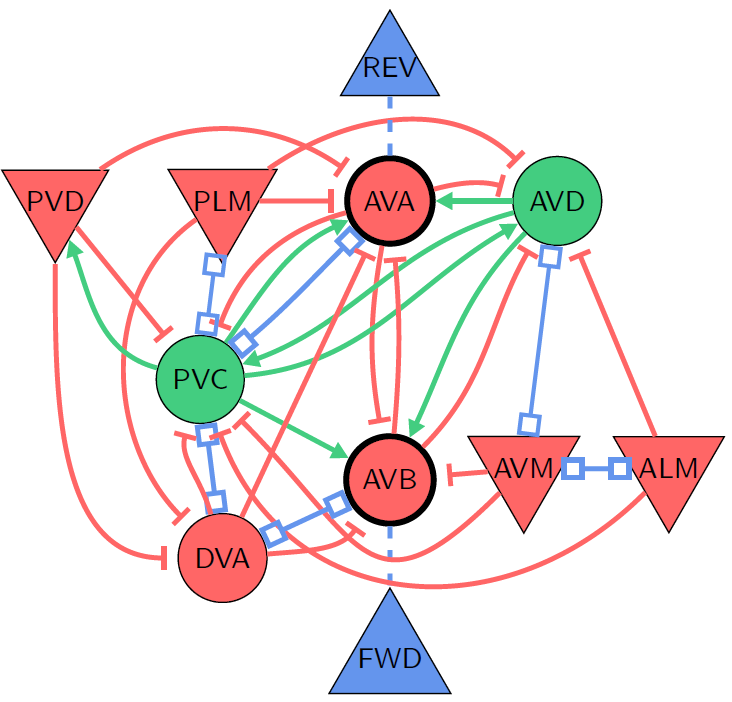
\includegraphics[width=4.8cm]{figures/nn_lechner.png}
  	\scalebox{0.23}{%% Creator: Matplotlib, PGF backend
%%
%% To include the figure in your LaTeX document, write
%%   \input{<filename>.pgf}
%%
%% Make sure the required packages are loaded in your preamble
%%   \usepackage{pgf}
%%
%% Figures using additional raster images can only be included by \input if
%% they are in the same directory as the main LaTeX file. For loading figures
%% from other directories you can use the `import` package
%%   \usepackage{import}
%% and then include the figures with
%%   \import{<path to file>}{<filename>.pgf}
%%
%% Matplotlib used the following preamble
%%   \usepackage{fontspec}
%%   \setmainfont{Times New Roman}
%%   \setsansfont{Verdana}
%%   \setmonofont{Courier New}
%%
\begingroup%
\makeatletter%
\begin{pgfpicture}%
\pgfpathrectangle{\pgfpointorigin}{\pgfqpoint{15.360000in}{7.670000in}}%
\pgfusepath{use as bounding box, clip}%
\begin{pgfscope}%
\pgfsetbuttcap%
\pgfsetmiterjoin%
\definecolor{currentfill}{rgb}{1.000000,1.000000,1.000000}%
\pgfsetfillcolor{currentfill}%
\pgfsetlinewidth{0.000000pt}%
\definecolor{currentstroke}{rgb}{1.000000,1.000000,1.000000}%
\pgfsetstrokecolor{currentstroke}%
\pgfsetdash{}{0pt}%
\pgfpathmoveto{\pgfqpoint{0.000000in}{0.000000in}}%
\pgfpathlineto{\pgfqpoint{15.360000in}{0.000000in}}%
\pgfpathlineto{\pgfqpoint{15.360000in}{7.670000in}}%
\pgfpathlineto{\pgfqpoint{0.000000in}{7.670000in}}%
\pgfpathclose%
\pgfusepath{fill}%
\end{pgfscope}%
\begin{pgfscope}%
\pgfsetbuttcap%
\pgfsetmiterjoin%
\definecolor{currentfill}{rgb}{1.000000,1.000000,1.000000}%
\pgfsetfillcolor{currentfill}%
\pgfsetlinewidth{0.000000pt}%
\definecolor{currentstroke}{rgb}{0.000000,0.000000,0.000000}%
\pgfsetstrokecolor{currentstroke}%
\pgfsetstrokeopacity{0.000000}%
\pgfsetdash{}{0pt}%
\pgfpathmoveto{\pgfqpoint{1.920000in}{0.843700in}}%
\pgfpathlineto{\pgfqpoint{7.330909in}{0.843700in}}%
\pgfpathlineto{\pgfqpoint{7.330909in}{6.749600in}}%
\pgfpathlineto{\pgfqpoint{1.920000in}{6.749600in}}%
\pgfpathclose%
\pgfusepath{fill}%
\end{pgfscope}%
\begin{pgfscope}%
\pgfsetbuttcap%
\pgfsetroundjoin%
\definecolor{currentfill}{rgb}{0.000000,0.000000,0.000000}%
\pgfsetfillcolor{currentfill}%
\pgfsetlinewidth{0.803000pt}%
\definecolor{currentstroke}{rgb}{0.000000,0.000000,0.000000}%
\pgfsetstrokecolor{currentstroke}%
\pgfsetdash{}{0pt}%
\pgfsys@defobject{currentmarker}{\pgfqpoint{0.000000in}{-0.048611in}}{\pgfqpoint{0.000000in}{0.000000in}}{%
\pgfpathmoveto{\pgfqpoint{0.000000in}{0.000000in}}%
\pgfpathlineto{\pgfqpoint{0.000000in}{-0.048611in}}%
\pgfusepath{stroke,fill}%
}%
\begin{pgfscope}%
\pgfsys@transformshift{2.165950in}{0.843700in}%
\pgfsys@useobject{currentmarker}{}%
\end{pgfscope}%
\end{pgfscope}%
\begin{pgfscope}%
\pgftext[x=2.165950in,y=0.746478in,,top]{\sffamily\fontsize{10.000000}{12.000000}\selectfont 0}%
\end{pgfscope}%
\begin{pgfscope}%
\pgfsetbuttcap%
\pgfsetroundjoin%
\definecolor{currentfill}{rgb}{0.000000,0.000000,0.000000}%
\pgfsetfillcolor{currentfill}%
\pgfsetlinewidth{0.803000pt}%
\definecolor{currentstroke}{rgb}{0.000000,0.000000,0.000000}%
\pgfsetstrokecolor{currentstroke}%
\pgfsetdash{}{0pt}%
\pgfsys@defobject{currentmarker}{\pgfqpoint{0.000000in}{-0.048611in}}{\pgfqpoint{0.000000in}{0.000000in}}{%
\pgfpathmoveto{\pgfqpoint{0.000000in}{0.000000in}}%
\pgfpathlineto{\pgfqpoint{0.000000in}{-0.048611in}}%
\pgfusepath{stroke,fill}%
}%
\begin{pgfscope}%
\pgfsys@transformshift{3.149949in}{0.843700in}%
\pgfsys@useobject{currentmarker}{}%
\end{pgfscope}%
\end{pgfscope}%
\begin{pgfscope}%
\pgftext[x=3.149949in,y=0.746478in,,top]{\sffamily\fontsize{10.000000}{12.000000}\selectfont 1000}%
\end{pgfscope}%
\begin{pgfscope}%
\pgfsetbuttcap%
\pgfsetroundjoin%
\definecolor{currentfill}{rgb}{0.000000,0.000000,0.000000}%
\pgfsetfillcolor{currentfill}%
\pgfsetlinewidth{0.803000pt}%
\definecolor{currentstroke}{rgb}{0.000000,0.000000,0.000000}%
\pgfsetstrokecolor{currentstroke}%
\pgfsetdash{}{0pt}%
\pgfsys@defobject{currentmarker}{\pgfqpoint{0.000000in}{-0.048611in}}{\pgfqpoint{0.000000in}{0.000000in}}{%
\pgfpathmoveto{\pgfqpoint{0.000000in}{0.000000in}}%
\pgfpathlineto{\pgfqpoint{0.000000in}{-0.048611in}}%
\pgfusepath{stroke,fill}%
}%
\begin{pgfscope}%
\pgfsys@transformshift{4.133947in}{0.843700in}%
\pgfsys@useobject{currentmarker}{}%
\end{pgfscope}%
\end{pgfscope}%
\begin{pgfscope}%
\pgftext[x=4.133947in,y=0.746478in,,top]{\sffamily\fontsize{10.000000}{12.000000}\selectfont 2000}%
\end{pgfscope}%
\begin{pgfscope}%
\pgfsetbuttcap%
\pgfsetroundjoin%
\definecolor{currentfill}{rgb}{0.000000,0.000000,0.000000}%
\pgfsetfillcolor{currentfill}%
\pgfsetlinewidth{0.803000pt}%
\definecolor{currentstroke}{rgb}{0.000000,0.000000,0.000000}%
\pgfsetstrokecolor{currentstroke}%
\pgfsetdash{}{0pt}%
\pgfsys@defobject{currentmarker}{\pgfqpoint{0.000000in}{-0.048611in}}{\pgfqpoint{0.000000in}{0.000000in}}{%
\pgfpathmoveto{\pgfqpoint{0.000000in}{0.000000in}}%
\pgfpathlineto{\pgfqpoint{0.000000in}{-0.048611in}}%
\pgfusepath{stroke,fill}%
}%
\begin{pgfscope}%
\pgfsys@transformshift{5.117946in}{0.843700in}%
\pgfsys@useobject{currentmarker}{}%
\end{pgfscope}%
\end{pgfscope}%
\begin{pgfscope}%
\pgftext[x=5.117946in,y=0.746478in,,top]{\sffamily\fontsize{10.000000}{12.000000}\selectfont 3000}%
\end{pgfscope}%
\begin{pgfscope}%
\pgfsetbuttcap%
\pgfsetroundjoin%
\definecolor{currentfill}{rgb}{0.000000,0.000000,0.000000}%
\pgfsetfillcolor{currentfill}%
\pgfsetlinewidth{0.803000pt}%
\definecolor{currentstroke}{rgb}{0.000000,0.000000,0.000000}%
\pgfsetstrokecolor{currentstroke}%
\pgfsetdash{}{0pt}%
\pgfsys@defobject{currentmarker}{\pgfqpoint{0.000000in}{-0.048611in}}{\pgfqpoint{0.000000in}{0.000000in}}{%
\pgfpathmoveto{\pgfqpoint{0.000000in}{0.000000in}}%
\pgfpathlineto{\pgfqpoint{0.000000in}{-0.048611in}}%
\pgfusepath{stroke,fill}%
}%
\begin{pgfscope}%
\pgfsys@transformshift{6.101944in}{0.843700in}%
\pgfsys@useobject{currentmarker}{}%
\end{pgfscope}%
\end{pgfscope}%
\begin{pgfscope}%
\pgftext[x=6.101944in,y=0.746478in,,top]{\sffamily\fontsize{10.000000}{12.000000}\selectfont 4000}%
\end{pgfscope}%
\begin{pgfscope}%
\pgfsetbuttcap%
\pgfsetroundjoin%
\definecolor{currentfill}{rgb}{0.000000,0.000000,0.000000}%
\pgfsetfillcolor{currentfill}%
\pgfsetlinewidth{0.803000pt}%
\definecolor{currentstroke}{rgb}{0.000000,0.000000,0.000000}%
\pgfsetstrokecolor{currentstroke}%
\pgfsetdash{}{0pt}%
\pgfsys@defobject{currentmarker}{\pgfqpoint{0.000000in}{-0.048611in}}{\pgfqpoint{0.000000in}{0.000000in}}{%
\pgfpathmoveto{\pgfqpoint{0.000000in}{0.000000in}}%
\pgfpathlineto{\pgfqpoint{0.000000in}{-0.048611in}}%
\pgfusepath{stroke,fill}%
}%
\begin{pgfscope}%
\pgfsys@transformshift{7.085943in}{0.843700in}%
\pgfsys@useobject{currentmarker}{}%
\end{pgfscope}%
\end{pgfscope}%
\begin{pgfscope}%
\pgftext[x=7.085943in,y=0.746478in,,top]{\sffamily\fontsize{10.000000}{12.000000}\selectfont 5000}%
\end{pgfscope}%
\begin{pgfscope}%
\pgftext[x=4.625455in,y=0.557459in,,top]{\sffamily\fontsize{10.000000}{12.000000}\selectfont t (in s)}%
\end{pgfscope}%
\begin{pgfscope}%
\pgfsetbuttcap%
\pgfsetroundjoin%
\definecolor{currentfill}{rgb}{0.000000,0.000000,0.000000}%
\pgfsetfillcolor{currentfill}%
\pgfsetlinewidth{0.803000pt}%
\definecolor{currentstroke}{rgb}{0.000000,0.000000,0.000000}%
\pgfsetstrokecolor{currentstroke}%
\pgfsetdash{}{0pt}%
\pgfsys@defobject{currentmarker}{\pgfqpoint{-0.048611in}{0.000000in}}{\pgfqpoint{0.000000in}{0.000000in}}{%
\pgfpathmoveto{\pgfqpoint{0.000000in}{0.000000in}}%
\pgfpathlineto{\pgfqpoint{-0.048611in}{0.000000in}}%
\pgfusepath{stroke,fill}%
}%
\begin{pgfscope}%
\pgfsys@transformshift{1.920000in}{1.495650in}%
\pgfsys@useobject{currentmarker}{}%
\end{pgfscope}%
\end{pgfscope}%
\begin{pgfscope}%
\pgftext[x=1.532522in,y=1.442888in,left,base]{\sffamily\fontsize{10.000000}{12.000000}\selectfont −73}%
\end{pgfscope}%
\begin{pgfscope}%
\pgfsetbuttcap%
\pgfsetroundjoin%
\definecolor{currentfill}{rgb}{0.000000,0.000000,0.000000}%
\pgfsetfillcolor{currentfill}%
\pgfsetlinewidth{0.803000pt}%
\definecolor{currentstroke}{rgb}{0.000000,0.000000,0.000000}%
\pgfsetstrokecolor{currentstroke}%
\pgfsetdash{}{0pt}%
\pgfsys@defobject{currentmarker}{\pgfqpoint{-0.048611in}{0.000000in}}{\pgfqpoint{0.000000in}{0.000000in}}{%
\pgfpathmoveto{\pgfqpoint{0.000000in}{0.000000in}}%
\pgfpathlineto{\pgfqpoint{-0.048611in}{0.000000in}}%
\pgfusepath{stroke,fill}%
}%
\begin{pgfscope}%
\pgfsys@transformshift{1.920000in}{2.262650in}%
\pgfsys@useobject{currentmarker}{}%
\end{pgfscope}%
\end{pgfscope}%
\begin{pgfscope}%
\pgftext[x=1.532522in,y=2.209888in,left,base]{\sffamily\fontsize{10.000000}{12.000000}\selectfont −72}%
\end{pgfscope}%
\begin{pgfscope}%
\pgfsetbuttcap%
\pgfsetroundjoin%
\definecolor{currentfill}{rgb}{0.000000,0.000000,0.000000}%
\pgfsetfillcolor{currentfill}%
\pgfsetlinewidth{0.803000pt}%
\definecolor{currentstroke}{rgb}{0.000000,0.000000,0.000000}%
\pgfsetstrokecolor{currentstroke}%
\pgfsetdash{}{0pt}%
\pgfsys@defobject{currentmarker}{\pgfqpoint{-0.048611in}{0.000000in}}{\pgfqpoint{0.000000in}{0.000000in}}{%
\pgfpathmoveto{\pgfqpoint{0.000000in}{0.000000in}}%
\pgfpathlineto{\pgfqpoint{-0.048611in}{0.000000in}}%
\pgfusepath{stroke,fill}%
}%
\begin{pgfscope}%
\pgfsys@transformshift{1.920000in}{3.029650in}%
\pgfsys@useobject{currentmarker}{}%
\end{pgfscope}%
\end{pgfscope}%
\begin{pgfscope}%
\pgftext[x=1.532522in,y=2.976888in,left,base]{\sffamily\fontsize{10.000000}{12.000000}\selectfont −71}%
\end{pgfscope}%
\begin{pgfscope}%
\pgfsetbuttcap%
\pgfsetroundjoin%
\definecolor{currentfill}{rgb}{0.000000,0.000000,0.000000}%
\pgfsetfillcolor{currentfill}%
\pgfsetlinewidth{0.803000pt}%
\definecolor{currentstroke}{rgb}{0.000000,0.000000,0.000000}%
\pgfsetstrokecolor{currentstroke}%
\pgfsetdash{}{0pt}%
\pgfsys@defobject{currentmarker}{\pgfqpoint{-0.048611in}{0.000000in}}{\pgfqpoint{0.000000in}{0.000000in}}{%
\pgfpathmoveto{\pgfqpoint{0.000000in}{0.000000in}}%
\pgfpathlineto{\pgfqpoint{-0.048611in}{0.000000in}}%
\pgfusepath{stroke,fill}%
}%
\begin{pgfscope}%
\pgfsys@transformshift{1.920000in}{3.796650in}%
\pgfsys@useobject{currentmarker}{}%
\end{pgfscope}%
\end{pgfscope}%
\begin{pgfscope}%
\pgftext[x=1.532522in,y=3.743888in,left,base]{\sffamily\fontsize{10.000000}{12.000000}\selectfont −70}%
\end{pgfscope}%
\begin{pgfscope}%
\pgfsetbuttcap%
\pgfsetroundjoin%
\definecolor{currentfill}{rgb}{0.000000,0.000000,0.000000}%
\pgfsetfillcolor{currentfill}%
\pgfsetlinewidth{0.803000pt}%
\definecolor{currentstroke}{rgb}{0.000000,0.000000,0.000000}%
\pgfsetstrokecolor{currentstroke}%
\pgfsetdash{}{0pt}%
\pgfsys@defobject{currentmarker}{\pgfqpoint{-0.048611in}{0.000000in}}{\pgfqpoint{0.000000in}{0.000000in}}{%
\pgfpathmoveto{\pgfqpoint{0.000000in}{0.000000in}}%
\pgfpathlineto{\pgfqpoint{-0.048611in}{0.000000in}}%
\pgfusepath{stroke,fill}%
}%
\begin{pgfscope}%
\pgfsys@transformshift{1.920000in}{4.563650in}%
\pgfsys@useobject{currentmarker}{}%
\end{pgfscope}%
\end{pgfscope}%
\begin{pgfscope}%
\pgftext[x=1.532522in,y=4.510888in,left,base]{\sffamily\fontsize{10.000000}{12.000000}\selectfont −69}%
\end{pgfscope}%
\begin{pgfscope}%
\pgfsetbuttcap%
\pgfsetroundjoin%
\definecolor{currentfill}{rgb}{0.000000,0.000000,0.000000}%
\pgfsetfillcolor{currentfill}%
\pgfsetlinewidth{0.803000pt}%
\definecolor{currentstroke}{rgb}{0.000000,0.000000,0.000000}%
\pgfsetstrokecolor{currentstroke}%
\pgfsetdash{}{0pt}%
\pgfsys@defobject{currentmarker}{\pgfqpoint{-0.048611in}{0.000000in}}{\pgfqpoint{0.000000in}{0.000000in}}{%
\pgfpathmoveto{\pgfqpoint{0.000000in}{0.000000in}}%
\pgfpathlineto{\pgfqpoint{-0.048611in}{0.000000in}}%
\pgfusepath{stroke,fill}%
}%
\begin{pgfscope}%
\pgfsys@transformshift{1.920000in}{5.330650in}%
\pgfsys@useobject{currentmarker}{}%
\end{pgfscope}%
\end{pgfscope}%
\begin{pgfscope}%
\pgftext[x=1.532522in,y=5.277888in,left,base]{\sffamily\fontsize{10.000000}{12.000000}\selectfont −68}%
\end{pgfscope}%
\begin{pgfscope}%
\pgfsetbuttcap%
\pgfsetroundjoin%
\definecolor{currentfill}{rgb}{0.000000,0.000000,0.000000}%
\pgfsetfillcolor{currentfill}%
\pgfsetlinewidth{0.803000pt}%
\definecolor{currentstroke}{rgb}{0.000000,0.000000,0.000000}%
\pgfsetstrokecolor{currentstroke}%
\pgfsetdash{}{0pt}%
\pgfsys@defobject{currentmarker}{\pgfqpoint{-0.048611in}{0.000000in}}{\pgfqpoint{0.000000in}{0.000000in}}{%
\pgfpathmoveto{\pgfqpoint{0.000000in}{0.000000in}}%
\pgfpathlineto{\pgfqpoint{-0.048611in}{0.000000in}}%
\pgfusepath{stroke,fill}%
}%
\begin{pgfscope}%
\pgfsys@transformshift{1.920000in}{6.097650in}%
\pgfsys@useobject{currentmarker}{}%
\end{pgfscope}%
\end{pgfscope}%
\begin{pgfscope}%
\pgftext[x=1.532522in,y=6.044888in,left,base]{\sffamily\fontsize{10.000000}{12.000000}\selectfont −67}%
\end{pgfscope}%
\begin{pgfscope}%
\pgftext[x=1.476966in,y=3.796650in,,bottom,rotate=90.000000]{\sffamily\fontsize{10.000000}{12.000000}\selectfont u(t) in [mV]}%
\end{pgfscope}%
\begin{pgfscope}%
\pgfpathrectangle{\pgfqpoint{1.920000in}{0.843700in}}{\pgfqpoint{5.410909in}{5.905900in}}%
\pgfusepath{clip}%
\pgfsetrectcap%
\pgfsetroundjoin%
\pgfsetlinewidth{1.003750pt}%
\definecolor{currentstroke}{rgb}{0.000000,0.000000,1.000000}%
\pgfsetstrokecolor{currentstroke}%
\pgfsetdash{}{0pt}%
\pgfpathmoveto{\pgfqpoint{2.165950in}{3.796650in}}%
\pgfpathlineto{\pgfqpoint{7.084959in}{3.796650in}}%
\pgfpathlineto{\pgfqpoint{7.084959in}{3.796650in}}%
\pgfusepath{stroke}%
\end{pgfscope}%
\begin{pgfscope}%
\pgfpathrectangle{\pgfqpoint{1.920000in}{0.843700in}}{\pgfqpoint{5.410909in}{5.905900in}}%
\pgfusepath{clip}%
\pgfsetrectcap%
\pgfsetroundjoin%
\pgfsetlinewidth{1.003750pt}%
\definecolor{currentstroke}{rgb}{0.750000,0.750000,0.000000}%
\pgfsetstrokecolor{currentstroke}%
\pgfsetdash{}{0pt}%
\pgfpathmoveto{\pgfqpoint{2.165950in}{3.796650in}}%
\pgfpathlineto{\pgfqpoint{7.084959in}{3.796650in}}%
\pgfpathlineto{\pgfqpoint{7.084959in}{3.796650in}}%
\pgfusepath{stroke}%
\end{pgfscope}%
\begin{pgfscope}%
\pgfpathrectangle{\pgfqpoint{1.920000in}{0.843700in}}{\pgfqpoint{5.410909in}{5.905900in}}%
\pgfusepath{clip}%
\pgfsetrectcap%
\pgfsetroundjoin%
\pgfsetlinewidth{1.003750pt}%
\definecolor{currentstroke}{rgb}{0.000000,0.500000,0.000000}%
\pgfsetstrokecolor{currentstroke}%
\pgfsetdash{}{0pt}%
\pgfpathmoveto{\pgfqpoint{2.165950in}{3.796650in}}%
\pgfpathlineto{\pgfqpoint{7.084959in}{3.796650in}}%
\pgfpathlineto{\pgfqpoint{7.084959in}{3.796650in}}%
\pgfusepath{stroke}%
\end{pgfscope}%
\begin{pgfscope}%
\pgfpathrectangle{\pgfqpoint{1.920000in}{0.843700in}}{\pgfqpoint{5.410909in}{5.905900in}}%
\pgfusepath{clip}%
\pgfsetrectcap%
\pgfsetroundjoin%
\pgfsetlinewidth{1.003750pt}%
\definecolor{currentstroke}{rgb}{1.000000,0.000000,0.000000}%
\pgfsetstrokecolor{currentstroke}%
\pgfsetdash{}{0pt}%
\pgfpathmoveto{\pgfqpoint{2.165950in}{3.796650in}}%
\pgfpathlineto{\pgfqpoint{7.084959in}{3.796650in}}%
\pgfpathlineto{\pgfqpoint{7.084959in}{3.796650in}}%
\pgfusepath{stroke}%
\end{pgfscope}%
\begin{pgfscope}%
\pgfsetrectcap%
\pgfsetmiterjoin%
\pgfsetlinewidth{0.803000pt}%
\definecolor{currentstroke}{rgb}{0.000000,0.000000,0.000000}%
\pgfsetstrokecolor{currentstroke}%
\pgfsetdash{}{0pt}%
\pgfpathmoveto{\pgfqpoint{1.920000in}{0.843700in}}%
\pgfpathlineto{\pgfqpoint{1.920000in}{6.749600in}}%
\pgfusepath{stroke}%
\end{pgfscope}%
\begin{pgfscope}%
\pgfsetrectcap%
\pgfsetmiterjoin%
\pgfsetlinewidth{0.803000pt}%
\definecolor{currentstroke}{rgb}{0.000000,0.000000,0.000000}%
\pgfsetstrokecolor{currentstroke}%
\pgfsetdash{}{0pt}%
\pgfpathmoveto{\pgfqpoint{7.330909in}{0.843700in}}%
\pgfpathlineto{\pgfqpoint{7.330909in}{6.749600in}}%
\pgfusepath{stroke}%
\end{pgfscope}%
\begin{pgfscope}%
\pgfsetrectcap%
\pgfsetmiterjoin%
\pgfsetlinewidth{0.803000pt}%
\definecolor{currentstroke}{rgb}{0.000000,0.000000,0.000000}%
\pgfsetstrokecolor{currentstroke}%
\pgfsetdash{}{0pt}%
\pgfpathmoveto{\pgfqpoint{1.920000in}{0.843700in}}%
\pgfpathlineto{\pgfqpoint{7.330909in}{0.843700in}}%
\pgfusepath{stroke}%
\end{pgfscope}%
\begin{pgfscope}%
\pgfsetrectcap%
\pgfsetmiterjoin%
\pgfsetlinewidth{0.803000pt}%
\definecolor{currentstroke}{rgb}{0.000000,0.000000,0.000000}%
\pgfsetstrokecolor{currentstroke}%
\pgfsetdash{}{0pt}%
\pgfpathmoveto{\pgfqpoint{1.920000in}{6.749600in}}%
\pgfpathlineto{\pgfqpoint{7.330909in}{6.749600in}}%
\pgfusepath{stroke}%
\end{pgfscope}%
\begin{pgfscope}%
\pgftext[x=4.625455in,y=6.832933in,,base]{\sffamily\fontsize{10.000000}{12.000000}\selectfont Sensory Neurons}%
\end{pgfscope}%
\begin{pgfscope}%
\pgfsetbuttcap%
\pgfsetmiterjoin%
\definecolor{currentfill}{rgb}{1.000000,1.000000,1.000000}%
\pgfsetfillcolor{currentfill}%
\pgfsetfillopacity{0.800000}%
\pgfsetlinewidth{1.003750pt}%
\definecolor{currentstroke}{rgb}{0.800000,0.800000,0.800000}%
\pgfsetstrokecolor{currentstroke}%
\pgfsetstrokeopacity{0.800000}%
\pgfsetdash{}{0pt}%
\pgfpathmoveto{\pgfqpoint{2.017222in}{5.826858in}}%
\pgfpathlineto{\pgfqpoint{2.764537in}{5.826858in}}%
\pgfpathquadraticcurveto{\pgfqpoint{2.792314in}{5.826858in}}{\pgfqpoint{2.792314in}{5.854636in}}%
\pgfpathlineto{\pgfqpoint{2.792314in}{6.652378in}}%
\pgfpathquadraticcurveto{\pgfqpoint{2.792314in}{6.680156in}}{\pgfqpoint{2.764537in}{6.680156in}}%
\pgfpathlineto{\pgfqpoint{2.017222in}{6.680156in}}%
\pgfpathquadraticcurveto{\pgfqpoint{1.989444in}{6.680156in}}{\pgfqpoint{1.989444in}{6.652378in}}%
\pgfpathlineto{\pgfqpoint{1.989444in}{5.854636in}}%
\pgfpathquadraticcurveto{\pgfqpoint{1.989444in}{5.826858in}}{\pgfqpoint{2.017222in}{5.826858in}}%
\pgfpathclose%
\pgfusepath{stroke,fill}%
\end{pgfscope}%
\begin{pgfscope}%
\pgfsetrectcap%
\pgfsetroundjoin%
\pgfsetlinewidth{1.003750pt}%
\definecolor{currentstroke}{rgb}{0.000000,0.000000,1.000000}%
\pgfsetstrokecolor{currentstroke}%
\pgfsetdash{}{0pt}%
\pgfpathmoveto{\pgfqpoint{2.045000in}{6.567688in}}%
\pgfpathlineto{\pgfqpoint{2.322778in}{6.567688in}}%
\pgfusepath{stroke}%
\end{pgfscope}%
\begin{pgfscope}%
\pgftext[x=2.433889in,y=6.519077in,left,base]{\sffamily\fontsize{10.000000}{12.000000}\selectfont PVD}%
\end{pgfscope}%
\begin{pgfscope}%
\pgfsetrectcap%
\pgfsetroundjoin%
\pgfsetlinewidth{1.003750pt}%
\definecolor{currentstroke}{rgb}{0.750000,0.750000,0.000000}%
\pgfsetstrokecolor{currentstroke}%
\pgfsetdash{}{0pt}%
\pgfpathmoveto{\pgfqpoint{2.045000in}{6.364780in}}%
\pgfpathlineto{\pgfqpoint{2.322778in}{6.364780in}}%
\pgfusepath{stroke}%
\end{pgfscope}%
\begin{pgfscope}%
\pgftext[x=2.433889in,y=6.316169in,left,base]{\sffamily\fontsize{10.000000}{12.000000}\selectfont PLM}%
\end{pgfscope}%
\begin{pgfscope}%
\pgfsetrectcap%
\pgfsetroundjoin%
\pgfsetlinewidth{1.003750pt}%
\definecolor{currentstroke}{rgb}{0.000000,0.500000,0.000000}%
\pgfsetstrokecolor{currentstroke}%
\pgfsetdash{}{0pt}%
\pgfpathmoveto{\pgfqpoint{2.045000in}{6.161872in}}%
\pgfpathlineto{\pgfqpoint{2.322778in}{6.161872in}}%
\pgfusepath{stroke}%
\end{pgfscope}%
\begin{pgfscope}%
\pgftext[x=2.433889in,y=6.113261in,left,base]{\sffamily\fontsize{10.000000}{12.000000}\selectfont AVM}%
\end{pgfscope}%
\begin{pgfscope}%
\pgfsetrectcap%
\pgfsetroundjoin%
\pgfsetlinewidth{1.003750pt}%
\definecolor{currentstroke}{rgb}{1.000000,0.000000,0.000000}%
\pgfsetstrokecolor{currentstroke}%
\pgfsetdash{}{0pt}%
\pgfpathmoveto{\pgfqpoint{2.045000in}{5.958965in}}%
\pgfpathlineto{\pgfqpoint{2.322778in}{5.958965in}}%
\pgfusepath{stroke}%
\end{pgfscope}%
\begin{pgfscope}%
\pgftext[x=2.433889in,y=5.910354in,left,base]{\sffamily\fontsize{10.000000}{12.000000}\selectfont ALM}%
\end{pgfscope}%
\begin{pgfscope}%
\pgfsetbuttcap%
\pgfsetmiterjoin%
\definecolor{currentfill}{rgb}{1.000000,1.000000,1.000000}%
\pgfsetfillcolor{currentfill}%
\pgfsetlinewidth{0.000000pt}%
\definecolor{currentstroke}{rgb}{0.000000,0.000000,0.000000}%
\pgfsetstrokecolor{currentstroke}%
\pgfsetstrokeopacity{0.000000}%
\pgfsetdash{}{0pt}%
\pgfpathmoveto{\pgfqpoint{8.413091in}{0.843700in}}%
\pgfpathlineto{\pgfqpoint{13.824000in}{0.843700in}}%
\pgfpathlineto{\pgfqpoint{13.824000in}{6.749600in}}%
\pgfpathlineto{\pgfqpoint{8.413091in}{6.749600in}}%
\pgfpathclose%
\pgfusepath{fill}%
\end{pgfscope}%
\begin{pgfscope}%
\pgfsetbuttcap%
\pgfsetroundjoin%
\definecolor{currentfill}{rgb}{0.000000,0.000000,0.000000}%
\pgfsetfillcolor{currentfill}%
\pgfsetlinewidth{0.803000pt}%
\definecolor{currentstroke}{rgb}{0.000000,0.000000,0.000000}%
\pgfsetstrokecolor{currentstroke}%
\pgfsetdash{}{0pt}%
\pgfsys@defobject{currentmarker}{\pgfqpoint{0.000000in}{-0.048611in}}{\pgfqpoint{0.000000in}{0.000000in}}{%
\pgfpathmoveto{\pgfqpoint{0.000000in}{0.000000in}}%
\pgfpathlineto{\pgfqpoint{0.000000in}{-0.048611in}}%
\pgfusepath{stroke,fill}%
}%
\begin{pgfscope}%
\pgfsys@transformshift{8.659041in}{0.843700in}%
\pgfsys@useobject{currentmarker}{}%
\end{pgfscope}%
\end{pgfscope}%
\begin{pgfscope}%
\pgftext[x=8.659041in,y=0.746478in,,top]{\sffamily\fontsize{10.000000}{12.000000}\selectfont 0}%
\end{pgfscope}%
\begin{pgfscope}%
\pgfsetbuttcap%
\pgfsetroundjoin%
\definecolor{currentfill}{rgb}{0.000000,0.000000,0.000000}%
\pgfsetfillcolor{currentfill}%
\pgfsetlinewidth{0.803000pt}%
\definecolor{currentstroke}{rgb}{0.000000,0.000000,0.000000}%
\pgfsetstrokecolor{currentstroke}%
\pgfsetdash{}{0pt}%
\pgfsys@defobject{currentmarker}{\pgfqpoint{0.000000in}{-0.048611in}}{\pgfqpoint{0.000000in}{0.000000in}}{%
\pgfpathmoveto{\pgfqpoint{0.000000in}{0.000000in}}%
\pgfpathlineto{\pgfqpoint{0.000000in}{-0.048611in}}%
\pgfusepath{stroke,fill}%
}%
\begin{pgfscope}%
\pgfsys@transformshift{9.642843in}{0.843700in}%
\pgfsys@useobject{currentmarker}{}%
\end{pgfscope}%
\end{pgfscope}%
\begin{pgfscope}%
\pgftext[x=9.642843in,y=0.746478in,,top]{\sffamily\fontsize{10.000000}{12.000000}\selectfont 1000}%
\end{pgfscope}%
\begin{pgfscope}%
\pgfsetbuttcap%
\pgfsetroundjoin%
\definecolor{currentfill}{rgb}{0.000000,0.000000,0.000000}%
\pgfsetfillcolor{currentfill}%
\pgfsetlinewidth{0.803000pt}%
\definecolor{currentstroke}{rgb}{0.000000,0.000000,0.000000}%
\pgfsetstrokecolor{currentstroke}%
\pgfsetdash{}{0pt}%
\pgfsys@defobject{currentmarker}{\pgfqpoint{0.000000in}{-0.048611in}}{\pgfqpoint{0.000000in}{0.000000in}}{%
\pgfpathmoveto{\pgfqpoint{0.000000in}{0.000000in}}%
\pgfpathlineto{\pgfqpoint{0.000000in}{-0.048611in}}%
\pgfusepath{stroke,fill}%
}%
\begin{pgfscope}%
\pgfsys@transformshift{10.626645in}{0.843700in}%
\pgfsys@useobject{currentmarker}{}%
\end{pgfscope}%
\end{pgfscope}%
\begin{pgfscope}%
\pgftext[x=10.626645in,y=0.746478in,,top]{\sffamily\fontsize{10.000000}{12.000000}\selectfont 2000}%
\end{pgfscope}%
\begin{pgfscope}%
\pgfsetbuttcap%
\pgfsetroundjoin%
\definecolor{currentfill}{rgb}{0.000000,0.000000,0.000000}%
\pgfsetfillcolor{currentfill}%
\pgfsetlinewidth{0.803000pt}%
\definecolor{currentstroke}{rgb}{0.000000,0.000000,0.000000}%
\pgfsetstrokecolor{currentstroke}%
\pgfsetdash{}{0pt}%
\pgfsys@defobject{currentmarker}{\pgfqpoint{0.000000in}{-0.048611in}}{\pgfqpoint{0.000000in}{0.000000in}}{%
\pgfpathmoveto{\pgfqpoint{0.000000in}{0.000000in}}%
\pgfpathlineto{\pgfqpoint{0.000000in}{-0.048611in}}%
\pgfusepath{stroke,fill}%
}%
\begin{pgfscope}%
\pgfsys@transformshift{11.610446in}{0.843700in}%
\pgfsys@useobject{currentmarker}{}%
\end{pgfscope}%
\end{pgfscope}%
\begin{pgfscope}%
\pgftext[x=11.610446in,y=0.746478in,,top]{\sffamily\fontsize{10.000000}{12.000000}\selectfont 3000}%
\end{pgfscope}%
\begin{pgfscope}%
\pgfsetbuttcap%
\pgfsetroundjoin%
\definecolor{currentfill}{rgb}{0.000000,0.000000,0.000000}%
\pgfsetfillcolor{currentfill}%
\pgfsetlinewidth{0.803000pt}%
\definecolor{currentstroke}{rgb}{0.000000,0.000000,0.000000}%
\pgfsetstrokecolor{currentstroke}%
\pgfsetdash{}{0pt}%
\pgfsys@defobject{currentmarker}{\pgfqpoint{0.000000in}{-0.048611in}}{\pgfqpoint{0.000000in}{0.000000in}}{%
\pgfpathmoveto{\pgfqpoint{0.000000in}{0.000000in}}%
\pgfpathlineto{\pgfqpoint{0.000000in}{-0.048611in}}%
\pgfusepath{stroke,fill}%
}%
\begin{pgfscope}%
\pgfsys@transformshift{12.594248in}{0.843700in}%
\pgfsys@useobject{currentmarker}{}%
\end{pgfscope}%
\end{pgfscope}%
\begin{pgfscope}%
\pgftext[x=12.594248in,y=0.746478in,,top]{\sffamily\fontsize{10.000000}{12.000000}\selectfont 4000}%
\end{pgfscope}%
\begin{pgfscope}%
\pgfsetbuttcap%
\pgfsetroundjoin%
\definecolor{currentfill}{rgb}{0.000000,0.000000,0.000000}%
\pgfsetfillcolor{currentfill}%
\pgfsetlinewidth{0.803000pt}%
\definecolor{currentstroke}{rgb}{0.000000,0.000000,0.000000}%
\pgfsetstrokecolor{currentstroke}%
\pgfsetdash{}{0pt}%
\pgfsys@defobject{currentmarker}{\pgfqpoint{0.000000in}{-0.048611in}}{\pgfqpoint{0.000000in}{0.000000in}}{%
\pgfpathmoveto{\pgfqpoint{0.000000in}{0.000000in}}%
\pgfpathlineto{\pgfqpoint{0.000000in}{-0.048611in}}%
\pgfusepath{stroke,fill}%
}%
\begin{pgfscope}%
\pgfsys@transformshift{13.578050in}{0.843700in}%
\pgfsys@useobject{currentmarker}{}%
\end{pgfscope}%
\end{pgfscope}%
\begin{pgfscope}%
\pgftext[x=13.578050in,y=0.746478in,,top]{\sffamily\fontsize{10.000000}{12.000000}\selectfont 5000}%
\end{pgfscope}%
\begin{pgfscope}%
\pgftext[x=11.118545in,y=0.557459in,,top]{\sffamily\fontsize{10.000000}{12.000000}\selectfont t in [s]}%
\end{pgfscope}%
\begin{pgfscope}%
\pgfsetbuttcap%
\pgfsetroundjoin%
\definecolor{currentfill}{rgb}{0.000000,0.000000,0.000000}%
\pgfsetfillcolor{currentfill}%
\pgfsetlinewidth{0.803000pt}%
\definecolor{currentstroke}{rgb}{0.000000,0.000000,0.000000}%
\pgfsetstrokecolor{currentstroke}%
\pgfsetdash{}{0pt}%
\pgfsys@defobject{currentmarker}{\pgfqpoint{-0.048611in}{0.000000in}}{\pgfqpoint{0.000000in}{0.000000in}}{%
\pgfpathmoveto{\pgfqpoint{0.000000in}{0.000000in}}%
\pgfpathlineto{\pgfqpoint{-0.048611in}{0.000000in}}%
\pgfusepath{stroke,fill}%
}%
\begin{pgfscope}%
\pgfsys@transformshift{8.413091in}{1.515689in}%
\pgfsys@useobject{currentmarker}{}%
\end{pgfscope}%
\end{pgfscope}%
\begin{pgfscope}%
\pgftext[x=7.937315in,y=1.462928in,left,base]{\sffamily\fontsize{10.000000}{12.000000}\selectfont −300}%
\end{pgfscope}%
\begin{pgfscope}%
\pgfsetbuttcap%
\pgfsetroundjoin%
\definecolor{currentfill}{rgb}{0.000000,0.000000,0.000000}%
\pgfsetfillcolor{currentfill}%
\pgfsetlinewidth{0.803000pt}%
\definecolor{currentstroke}{rgb}{0.000000,0.000000,0.000000}%
\pgfsetstrokecolor{currentstroke}%
\pgfsetdash{}{0pt}%
\pgfsys@defobject{currentmarker}{\pgfqpoint{-0.048611in}{0.000000in}}{\pgfqpoint{0.000000in}{0.000000in}}{%
\pgfpathmoveto{\pgfqpoint{0.000000in}{0.000000in}}%
\pgfpathlineto{\pgfqpoint{-0.048611in}{0.000000in}}%
\pgfusepath{stroke,fill}%
}%
\begin{pgfscope}%
\pgfsys@transformshift{8.413091in}{2.401989in}%
\pgfsys@useobject{currentmarker}{}%
\end{pgfscope}%
\end{pgfscope}%
\begin{pgfscope}%
\pgftext[x=7.937315in,y=2.349227in,left,base]{\sffamily\fontsize{10.000000}{12.000000}\selectfont −250}%
\end{pgfscope}%
\begin{pgfscope}%
\pgfsetbuttcap%
\pgfsetroundjoin%
\definecolor{currentfill}{rgb}{0.000000,0.000000,0.000000}%
\pgfsetfillcolor{currentfill}%
\pgfsetlinewidth{0.803000pt}%
\definecolor{currentstroke}{rgb}{0.000000,0.000000,0.000000}%
\pgfsetstrokecolor{currentstroke}%
\pgfsetdash{}{0pt}%
\pgfsys@defobject{currentmarker}{\pgfqpoint{-0.048611in}{0.000000in}}{\pgfqpoint{0.000000in}{0.000000in}}{%
\pgfpathmoveto{\pgfqpoint{0.000000in}{0.000000in}}%
\pgfpathlineto{\pgfqpoint{-0.048611in}{0.000000in}}%
\pgfusepath{stroke,fill}%
}%
\begin{pgfscope}%
\pgfsys@transformshift{8.413091in}{3.288289in}%
\pgfsys@useobject{currentmarker}{}%
\end{pgfscope}%
\end{pgfscope}%
\begin{pgfscope}%
\pgftext[x=7.937315in,y=3.235527in,left,base]{\sffamily\fontsize{10.000000}{12.000000}\selectfont −200}%
\end{pgfscope}%
\begin{pgfscope}%
\pgfsetbuttcap%
\pgfsetroundjoin%
\definecolor{currentfill}{rgb}{0.000000,0.000000,0.000000}%
\pgfsetfillcolor{currentfill}%
\pgfsetlinewidth{0.803000pt}%
\definecolor{currentstroke}{rgb}{0.000000,0.000000,0.000000}%
\pgfsetstrokecolor{currentstroke}%
\pgfsetdash{}{0pt}%
\pgfsys@defobject{currentmarker}{\pgfqpoint{-0.048611in}{0.000000in}}{\pgfqpoint{0.000000in}{0.000000in}}{%
\pgfpathmoveto{\pgfqpoint{0.000000in}{0.000000in}}%
\pgfpathlineto{\pgfqpoint{-0.048611in}{0.000000in}}%
\pgfusepath{stroke,fill}%
}%
\begin{pgfscope}%
\pgfsys@transformshift{8.413091in}{4.174589in}%
\pgfsys@useobject{currentmarker}{}%
\end{pgfscope}%
\end{pgfscope}%
\begin{pgfscope}%
\pgftext[x=7.937315in,y=4.121827in,left,base]{\sffamily\fontsize{10.000000}{12.000000}\selectfont −150}%
\end{pgfscope}%
\begin{pgfscope}%
\pgfsetbuttcap%
\pgfsetroundjoin%
\definecolor{currentfill}{rgb}{0.000000,0.000000,0.000000}%
\pgfsetfillcolor{currentfill}%
\pgfsetlinewidth{0.803000pt}%
\definecolor{currentstroke}{rgb}{0.000000,0.000000,0.000000}%
\pgfsetstrokecolor{currentstroke}%
\pgfsetdash{}{0pt}%
\pgfsys@defobject{currentmarker}{\pgfqpoint{-0.048611in}{0.000000in}}{\pgfqpoint{0.000000in}{0.000000in}}{%
\pgfpathmoveto{\pgfqpoint{0.000000in}{0.000000in}}%
\pgfpathlineto{\pgfqpoint{-0.048611in}{0.000000in}}%
\pgfusepath{stroke,fill}%
}%
\begin{pgfscope}%
\pgfsys@transformshift{8.413091in}{5.060888in}%
\pgfsys@useobject{currentmarker}{}%
\end{pgfscope}%
\end{pgfscope}%
\begin{pgfscope}%
\pgftext[x=7.937315in,y=5.008127in,left,base]{\sffamily\fontsize{10.000000}{12.000000}\selectfont −100}%
\end{pgfscope}%
\begin{pgfscope}%
\pgfsetbuttcap%
\pgfsetroundjoin%
\definecolor{currentfill}{rgb}{0.000000,0.000000,0.000000}%
\pgfsetfillcolor{currentfill}%
\pgfsetlinewidth{0.803000pt}%
\definecolor{currentstroke}{rgb}{0.000000,0.000000,0.000000}%
\pgfsetstrokecolor{currentstroke}%
\pgfsetdash{}{0pt}%
\pgfsys@defobject{currentmarker}{\pgfqpoint{-0.048611in}{0.000000in}}{\pgfqpoint{0.000000in}{0.000000in}}{%
\pgfpathmoveto{\pgfqpoint{0.000000in}{0.000000in}}%
\pgfpathlineto{\pgfqpoint{-0.048611in}{0.000000in}}%
\pgfusepath{stroke,fill}%
}%
\begin{pgfscope}%
\pgfsys@transformshift{8.413091in}{5.947188in}%
\pgfsys@useobject{currentmarker}{}%
\end{pgfscope}%
\end{pgfscope}%
\begin{pgfscope}%
\pgftext[x=8.025613in,y=5.894427in,left,base]{\sffamily\fontsize{10.000000}{12.000000}\selectfont −50}%
\end{pgfscope}%
\begin{pgfscope}%
\pgftext[x=7.881760in,y=3.796650in,,bottom,rotate=90.000000]{\sffamily\fontsize{10.000000}{12.000000}\selectfont u(t) in [mV]}%
\end{pgfscope}%
\begin{pgfscope}%
\pgfpathrectangle{\pgfqpoint{8.413091in}{0.843700in}}{\pgfqpoint{5.410909in}{5.905900in}}%
\pgfusepath{clip}%
\pgfsetrectcap%
\pgfsetroundjoin%
\pgfsetlinewidth{1.003750pt}%
\definecolor{currentstroke}{rgb}{0.000000,0.000000,1.000000}%
\pgfsetstrokecolor{currentstroke}%
\pgfsetdash{}{0pt}%
\pgfpathmoveto{\pgfqpoint{8.659041in}{5.592668in}}%
\pgfpathlineto{\pgfqpoint{8.685604in}{5.637326in}}%
\pgfpathlineto{\pgfqpoint{8.712167in}{5.677675in}}%
\pgfpathlineto{\pgfqpoint{8.738729in}{5.714127in}}%
\pgfpathlineto{\pgfqpoint{8.766276in}{5.748209in}}%
\pgfpathlineto{\pgfqpoint{8.794806in}{5.779911in}}%
\pgfpathlineto{\pgfqpoint{8.823336in}{5.808320in}}%
\pgfpathlineto{\pgfqpoint{8.852850in}{5.834601in}}%
\pgfpathlineto{\pgfqpoint{8.883348in}{5.858786in}}%
\pgfpathlineto{\pgfqpoint{8.914830in}{5.880926in}}%
\pgfpathlineto{\pgfqpoint{8.947295in}{5.901086in}}%
\pgfpathlineto{\pgfqpoint{8.981728in}{5.919846in}}%
\pgfpathlineto{\pgfqpoint{9.018129in}{5.937095in}}%
\pgfpathlineto{\pgfqpoint{9.056497in}{5.952767in}}%
\pgfpathlineto{\pgfqpoint{9.096833in}{5.966835in}}%
\pgfpathlineto{\pgfqpoint{9.140120in}{5.979567in}}%
\pgfpathlineto{\pgfqpoint{9.187343in}{5.991078in}}%
\pgfpathlineto{\pgfqpoint{9.238500in}{6.001189in}}%
\pgfpathlineto{\pgfqpoint{9.294577in}{6.009931in}}%
\pgfpathlineto{\pgfqpoint{9.355573in}{6.017164in}}%
\pgfpathlineto{\pgfqpoint{9.424439in}{6.023038in}}%
\pgfpathlineto{\pgfqpoint{9.502159in}{6.027363in}}%
\pgfpathlineto{\pgfqpoint{9.590701in}{6.029999in}}%
\pgfpathlineto{\pgfqpoint{9.693017in}{6.030757in}}%
\pgfpathlineto{\pgfqpoint{9.813041in}{6.029347in}}%
\pgfpathlineto{\pgfqpoint{9.953724in}{6.025402in}}%
\pgfpathlineto{\pgfqpoint{10.117035in}{6.018550in}}%
\pgfpathlineto{\pgfqpoint{10.301990in}{6.008527in}}%
\pgfpathlineto{\pgfqpoint{10.500718in}{5.995520in}}%
\pgfpathlineto{\pgfqpoint{10.705349in}{5.979900in}}%
\pgfpathlineto{\pgfqpoint{10.908012in}{5.962215in}}%
\pgfpathlineto{\pgfqpoint{11.036890in}{5.951020in}}%
\pgfpathlineto{\pgfqpoint{11.066404in}{5.965264in}}%
\pgfpathlineto{\pgfqpoint{11.096902in}{5.977494in}}%
\pgfpathlineto{\pgfqpoint{11.129367in}{5.988056in}}%
\pgfpathlineto{\pgfqpoint{11.162817in}{5.996605in}}%
\pgfpathlineto{\pgfqpoint{11.199217in}{6.003563in}}%
\pgfpathlineto{\pgfqpoint{11.237585in}{6.008611in}}%
\pgfpathlineto{\pgfqpoint{11.278905in}{6.011804in}}%
\pgfpathlineto{\pgfqpoint{11.324160in}{6.013050in}}%
\pgfpathlineto{\pgfqpoint{11.374334in}{6.012154in}}%
\pgfpathlineto{\pgfqpoint{11.430411in}{6.008868in}}%
\pgfpathlineto{\pgfqpoint{11.494358in}{6.002851in}}%
\pgfpathlineto{\pgfqpoint{11.570110in}{5.993413in}}%
\pgfpathlineto{\pgfqpoint{11.661604in}{5.979689in}}%
\pgfpathlineto{\pgfqpoint{11.720632in}{5.971135in}}%
\pgfpathlineto{\pgfqpoint{11.749162in}{5.982909in}}%
\pgfpathlineto{\pgfqpoint{11.778676in}{5.992687in}}%
\pgfpathlineto{\pgfqpoint{11.810158in}{6.000735in}}%
\pgfpathlineto{\pgfqpoint{11.843607in}{6.006921in}}%
\pgfpathlineto{\pgfqpoint{11.879024in}{6.011159in}}%
\pgfpathlineto{\pgfqpoint{11.917392in}{6.013440in}}%
\pgfpathlineto{\pgfqpoint{11.958712in}{6.013615in}}%
\pgfpathlineto{\pgfqpoint{12.003967in}{6.011544in}}%
\pgfpathlineto{\pgfqpoint{12.054141in}{6.007005in}}%
\pgfpathlineto{\pgfqpoint{12.111201in}{5.999580in}}%
\pgfpathlineto{\pgfqpoint{12.178100in}{5.988548in}}%
\pgfpathlineto{\pgfqpoint{12.233193in}{5.979291in}}%
\pgfpathlineto{\pgfqpoint{12.260739in}{5.989852in}}%
\pgfpathlineto{\pgfqpoint{12.289269in}{5.998425in}}%
\pgfpathlineto{\pgfqpoint{12.319767in}{6.005231in}}%
\pgfpathlineto{\pgfqpoint{12.352233in}{6.010119in}}%
\pgfpathlineto{\pgfqpoint{12.386666in}{6.012990in}}%
\pgfpathlineto{\pgfqpoint{12.423066in}{6.013792in}}%
\pgfpathlineto{\pgfqpoint{12.463402in}{6.012410in}}%
\pgfpathlineto{\pgfqpoint{12.507673in}{6.008608in}}%
\pgfpathlineto{\pgfqpoint{12.556863in}{6.002102in}}%
\pgfpathlineto{\pgfqpoint{12.612940in}{5.992370in}}%
\pgfpathlineto{\pgfqpoint{12.659179in}{5.984134in}}%
\pgfpathlineto{\pgfqpoint{12.685741in}{5.993847in}}%
\pgfpathlineto{\pgfqpoint{12.713288in}{6.001600in}}%
\pgfpathlineto{\pgfqpoint{12.742802in}{6.007575in}}%
\pgfpathlineto{\pgfqpoint{12.774284in}{6.011604in}}%
\pgfpathlineto{\pgfqpoint{12.807733in}{6.013572in}}%
\pgfpathlineto{\pgfqpoint{12.843150in}{6.013418in}}%
\pgfpathlineto{\pgfqpoint{12.882502in}{6.010954in}}%
\pgfpathlineto{\pgfqpoint{12.924805in}{6.006057in}}%
\pgfpathlineto{\pgfqpoint{12.972028in}{5.998339in}}%
\pgfpathlineto{\pgfqpoint{13.026137in}{5.987169in}}%
\pgfpathlineto{\pgfqpoint{13.030072in}{5.986897in}}%
\pgfpathlineto{\pgfqpoint{13.055651in}{5.996040in}}%
\pgfpathlineto{\pgfqpoint{13.083197in}{6.003484in}}%
\pgfpathlineto{\pgfqpoint{13.111728in}{6.008856in}}%
\pgfpathlineto{\pgfqpoint{13.142225in}{6.012277in}}%
\pgfpathlineto{\pgfqpoint{13.174691in}{6.013616in}}%
\pgfpathlineto{\pgfqpoint{13.209124in}{6.012794in}}%
\pgfpathlineto{\pgfqpoint{13.246508in}{6.009669in}}%
\pgfpathlineto{\pgfqpoint{13.287828in}{6.003944in}}%
\pgfpathlineto{\pgfqpoint{13.334067in}{5.995211in}}%
\pgfpathlineto{\pgfqpoint{13.364565in}{5.989583in}}%
\pgfpathlineto{\pgfqpoint{13.390143in}{5.998377in}}%
\pgfpathlineto{\pgfqpoint{13.416706in}{6.005146in}}%
\pgfpathlineto{\pgfqpoint{13.444253in}{6.009897in}}%
\pgfpathlineto{\pgfqpoint{13.473767in}{6.012721in}}%
\pgfpathlineto{\pgfqpoint{13.505248in}{6.013467in}}%
\pgfpathlineto{\pgfqpoint{13.538698in}{6.012036in}}%
\pgfpathlineto{\pgfqpoint{13.575098in}{6.008247in}}%
\pgfpathlineto{\pgfqpoint{13.578050in}{6.007849in}}%
\pgfpathlineto{\pgfqpoint{13.578050in}{6.007849in}}%
\pgfusepath{stroke}%
\end{pgfscope}%
\begin{pgfscope}%
\pgfpathrectangle{\pgfqpoint{8.413091in}{0.843700in}}{\pgfqpoint{5.410909in}{5.905900in}}%
\pgfusepath{clip}%
\pgfsetrectcap%
\pgfsetroundjoin%
\pgfsetlinewidth{1.003750pt}%
\definecolor{currentstroke}{rgb}{0.750000,0.750000,0.000000}%
\pgfsetstrokecolor{currentstroke}%
\pgfsetdash{}{0pt}%
\pgfpathmoveto{\pgfqpoint{8.659041in}{5.592668in}}%
\pgfpathlineto{\pgfqpoint{8.690523in}{5.619030in}}%
\pgfpathlineto{\pgfqpoint{8.722988in}{5.643370in}}%
\pgfpathlineto{\pgfqpoint{8.757421in}{5.666365in}}%
\pgfpathlineto{\pgfqpoint{8.792838in}{5.687327in}}%
\pgfpathlineto{\pgfqpoint{8.830223in}{5.706836in}}%
\pgfpathlineto{\pgfqpoint{8.869575in}{5.724820in}}%
\pgfpathlineto{\pgfqpoint{8.910895in}{5.741245in}}%
\pgfpathlineto{\pgfqpoint{8.955166in}{5.756424in}}%
\pgfpathlineto{\pgfqpoint{9.002388in}{5.770247in}}%
\pgfpathlineto{\pgfqpoint{9.053546in}{5.782880in}}%
\pgfpathlineto{\pgfqpoint{9.109622in}{5.794387in}}%
\pgfpathlineto{\pgfqpoint{9.170618in}{5.804611in}}%
\pgfpathlineto{\pgfqpoint{9.238500in}{5.813720in}}%
\pgfpathlineto{\pgfqpoint{9.315237in}{5.821744in}}%
\pgfpathlineto{\pgfqpoint{9.403779in}{5.828706in}}%
\pgfpathlineto{\pgfqpoint{9.508062in}{5.834589in}}%
\pgfpathlineto{\pgfqpoint{9.633989in}{5.839372in}}%
\pgfpathlineto{\pgfqpoint{9.793365in}{5.843084in}}%
\pgfpathlineto{\pgfqpoint{10.008817in}{5.845736in}}%
\pgfpathlineto{\pgfqpoint{10.340358in}{5.847371in}}%
\pgfpathlineto{\pgfqpoint{11.025084in}{5.848060in}}%
\pgfpathlineto{\pgfqpoint{13.578050in}{5.848131in}}%
\pgfpathlineto{\pgfqpoint{13.578050in}{5.848131in}}%
\pgfusepath{stroke}%
\end{pgfscope}%
\begin{pgfscope}%
\pgfpathrectangle{\pgfqpoint{8.413091in}{0.843700in}}{\pgfqpoint{5.410909in}{5.905900in}}%
\pgfusepath{clip}%
\pgfsetrectcap%
\pgfsetroundjoin%
\pgfsetlinewidth{1.003750pt}%
\definecolor{currentstroke}{rgb}{0.000000,0.500000,0.000000}%
\pgfsetstrokecolor{currentstroke}%
\pgfsetdash{}{0pt}%
\pgfpathmoveto{\pgfqpoint{8.659041in}{5.592668in}}%
\pgfpathlineto{\pgfqpoint{8.690523in}{5.619038in}}%
\pgfpathlineto{\pgfqpoint{8.723972in}{5.644137in}}%
\pgfpathlineto{\pgfqpoint{8.759389in}{5.667854in}}%
\pgfpathlineto{\pgfqpoint{8.796774in}{5.690135in}}%
\pgfpathlineto{\pgfqpoint{8.836126in}{5.710980in}}%
\pgfpathlineto{\pgfqpoint{8.878429in}{5.730870in}}%
\pgfpathlineto{\pgfqpoint{8.924668in}{5.750135in}}%
\pgfpathlineto{\pgfqpoint{8.975825in}{5.769010in}}%
\pgfpathlineto{\pgfqpoint{9.033870in}{5.787991in}}%
\pgfpathlineto{\pgfqpoint{9.100768in}{5.807471in}}%
\pgfpathlineto{\pgfqpoint{9.182424in}{5.828854in}}%
\pgfpathlineto{\pgfqpoint{9.294577in}{5.855751in}}%
\pgfpathlineto{\pgfqpoint{9.670389in}{5.944228in}}%
\pgfpathlineto{\pgfqpoint{9.794348in}{5.976590in}}%
\pgfpathlineto{\pgfqpoint{9.909453in}{6.008912in}}%
\pgfpathlineto{\pgfqpoint{10.019639in}{6.042144in}}%
\pgfpathlineto{\pgfqpoint{10.126873in}{6.076801in}}%
\pgfpathlineto{\pgfqpoint{10.231156in}{6.112824in}}%
\pgfpathlineto{\pgfqpoint{10.333472in}{6.150497in}}%
\pgfpathlineto{\pgfqpoint{10.434803in}{6.190185in}}%
\pgfpathlineto{\pgfqpoint{10.534167in}{6.231496in}}%
\pgfpathlineto{\pgfqpoint{10.631564in}{6.274386in}}%
\pgfpathlineto{\pgfqpoint{10.727976in}{6.319278in}}%
\pgfpathlineto{\pgfqpoint{10.822421in}{6.365699in}}%
\pgfpathlineto{\pgfqpoint{10.915882in}{6.414122in}}%
\pgfpathlineto{\pgfqpoint{11.007376in}{6.464022in}}%
\pgfpathlineto{\pgfqpoint{11.033939in}{6.478986in}}%
\pgfpathlineto{\pgfqpoint{11.034922in}{5.592668in}}%
\pgfpathlineto{\pgfqpoint{11.035906in}{5.594379in}}%
\pgfpathlineto{\pgfqpoint{11.083129in}{5.674181in}}%
\pgfpathlineto{\pgfqpoint{11.132319in}{5.752888in}}%
\pgfpathlineto{\pgfqpoint{11.183476in}{5.830583in}}%
\pgfpathlineto{\pgfqpoint{11.238569in}{5.910160in}}%
\pgfpathlineto{\pgfqpoint{11.296614in}{5.990073in}}%
\pgfpathlineto{\pgfqpoint{11.359577in}{6.072918in}}%
\pgfpathlineto{\pgfqpoint{11.414670in}{6.142080in}}%
\pgfpathlineto{\pgfqpoint{11.474682in}{6.213783in}}%
\pgfpathlineto{\pgfqpoint{11.541580in}{6.290161in}}%
\pgfpathlineto{\pgfqpoint{11.617333in}{6.373199in}}%
\pgfpathlineto{\pgfqpoint{11.707843in}{6.469002in}}%
\pgfpathlineto{\pgfqpoint{11.717681in}{6.479250in}}%
\pgfpathlineto{\pgfqpoint{11.718664in}{5.592668in}}%
\pgfpathlineto{\pgfqpoint{11.719648in}{5.594845in}}%
\pgfpathlineto{\pgfqpoint{11.764903in}{5.692226in}}%
\pgfpathlineto{\pgfqpoint{11.812126in}{5.788623in}}%
\pgfpathlineto{\pgfqpoint{11.862300in}{5.885928in}}%
\pgfpathlineto{\pgfqpoint{11.914441in}{5.982185in}}%
\pgfpathlineto{\pgfqpoint{11.967566in}{6.075666in}}%
\pgfpathlineto{\pgfqpoint{12.019708in}{6.162733in}}%
\pgfpathlineto{\pgfqpoint{12.074801in}{6.250382in}}%
\pgfpathlineto{\pgfqpoint{12.134813in}{6.341641in}}%
\pgfpathlineto{\pgfqpoint{12.200727in}{6.437767in}}%
\pgfpathlineto{\pgfqpoint{12.230241in}{6.479654in}}%
\pgfpathlineto{\pgfqpoint{12.231225in}{5.592668in}}%
\pgfpathlineto{\pgfqpoint{12.232209in}{5.595207in}}%
\pgfpathlineto{\pgfqpoint{12.277464in}{5.708836in}}%
\pgfpathlineto{\pgfqpoint{12.324686in}{5.821351in}}%
\pgfpathlineto{\pgfqpoint{12.373876in}{5.932776in}}%
\pgfpathlineto{\pgfqpoint{12.422083in}{6.036668in}}%
\pgfpathlineto{\pgfqpoint{12.471273in}{6.137329in}}%
\pgfpathlineto{\pgfqpoint{12.523414in}{6.238944in}}%
\pgfpathlineto{\pgfqpoint{12.579491in}{6.343273in}}%
\pgfpathlineto{\pgfqpoint{12.639503in}{6.450165in}}%
\pgfpathlineto{\pgfqpoint{12.656227in}{6.479198in}}%
\pgfpathlineto{\pgfqpoint{12.657211in}{5.592668in}}%
\pgfpathlineto{\pgfqpoint{12.658195in}{5.595520in}}%
\pgfpathlineto{\pgfqpoint{12.703450in}{5.723159in}}%
\pgfpathlineto{\pgfqpoint{12.750672in}{5.849588in}}%
\pgfpathlineto{\pgfqpoint{12.797895in}{5.969696in}}%
\pgfpathlineto{\pgfqpoint{12.845117in}{6.083628in}}%
\pgfpathlineto{\pgfqpoint{12.895291in}{6.198778in}}%
\pgfpathlineto{\pgfqpoint{12.947433in}{6.312895in}}%
\pgfpathlineto{\pgfqpoint{13.003509in}{6.430245in}}%
\pgfpathlineto{\pgfqpoint{13.028104in}{6.480181in}}%
\pgfpathlineto{\pgfqpoint{13.029088in}{5.592668in}}%
\pgfpathlineto{\pgfqpoint{13.030072in}{5.595802in}}%
\pgfpathlineto{\pgfqpoint{13.075327in}{5.736112in}}%
\pgfpathlineto{\pgfqpoint{13.121566in}{5.872207in}}%
\pgfpathlineto{\pgfqpoint{13.166820in}{5.998492in}}%
\pgfpathlineto{\pgfqpoint{13.214043in}{6.123762in}}%
\pgfpathlineto{\pgfqpoint{13.264217in}{6.250524in}}%
\pgfpathlineto{\pgfqpoint{13.317342in}{6.378597in}}%
\pgfpathlineto{\pgfqpoint{13.361613in}{6.481150in}}%
\pgfpathlineto{\pgfqpoint{13.362597in}{5.592668in}}%
\pgfpathlineto{\pgfqpoint{13.363581in}{5.596064in}}%
\pgfpathlineto{\pgfqpoint{13.408836in}{5.748105in}}%
\pgfpathlineto{\pgfqpoint{13.453107in}{5.889097in}}%
\pgfpathlineto{\pgfqpoint{13.499345in}{6.028813in}}%
\pgfpathlineto{\pgfqpoint{13.547552in}{6.167283in}}%
\pgfpathlineto{\pgfqpoint{13.578050in}{6.251523in}}%
\pgfpathlineto{\pgfqpoint{13.578050in}{6.251523in}}%
\pgfusepath{stroke}%
\end{pgfscope}%
\begin{pgfscope}%
\pgfpathrectangle{\pgfqpoint{8.413091in}{0.843700in}}{\pgfqpoint{5.410909in}{5.905900in}}%
\pgfusepath{clip}%
\pgfsetrectcap%
\pgfsetroundjoin%
\pgfsetlinewidth{1.003750pt}%
\definecolor{currentstroke}{rgb}{1.000000,0.000000,0.000000}%
\pgfsetstrokecolor{currentstroke}%
\pgfsetdash{}{0pt}%
\pgfpathmoveto{\pgfqpoint{8.659041in}{5.592668in}}%
\pgfpathlineto{\pgfqpoint{8.694458in}{5.591562in}}%
\pgfpathlineto{\pgfqpoint{8.731843in}{5.588113in}}%
\pgfpathlineto{\pgfqpoint{8.771195in}{5.582241in}}%
\pgfpathlineto{\pgfqpoint{8.813498in}{5.573669in}}%
\pgfpathlineto{\pgfqpoint{8.858753in}{5.562225in}}%
\pgfpathlineto{\pgfqpoint{8.907943in}{5.547457in}}%
\pgfpathlineto{\pgfqpoint{8.961068in}{5.529136in}}%
\pgfpathlineto{\pgfqpoint{9.018129in}{5.507076in}}%
\pgfpathlineto{\pgfqpoint{9.080108in}{5.480682in}}%
\pgfpathlineto{\pgfqpoint{9.146023in}{5.450182in}}%
\pgfpathlineto{\pgfqpoint{9.216857in}{5.414939in}}%
\pgfpathlineto{\pgfqpoint{9.291626in}{5.375252in}}%
\pgfpathlineto{\pgfqpoint{9.370330in}{5.330951in}}%
\pgfpathlineto{\pgfqpoint{9.451985in}{5.282426in}}%
\pgfpathlineto{\pgfqpoint{9.535609in}{5.230137in}}%
\pgfpathlineto{\pgfqpoint{9.620216in}{5.174613in}}%
\pgfpathlineto{\pgfqpoint{9.705806in}{5.115763in}}%
\pgfpathlineto{\pgfqpoint{9.790413in}{5.054904in}}%
\pgfpathlineto{\pgfqpoint{9.875020in}{4.991309in}}%
\pgfpathlineto{\pgfqpoint{9.958643in}{4.925677in}}%
\pgfpathlineto{\pgfqpoint{10.041283in}{4.858006in}}%
\pgfpathlineto{\pgfqpoint{10.122938in}{4.788285in}}%
\pgfpathlineto{\pgfqpoint{10.203610in}{4.716500in}}%
\pgfpathlineto{\pgfqpoint{10.283298in}{4.642635in}}%
\pgfpathlineto{\pgfqpoint{10.362002in}{4.566675in}}%
\pgfpathlineto{\pgfqpoint{10.439722in}{4.488605in}}%
\pgfpathlineto{\pgfqpoint{10.517443in}{4.407365in}}%
\pgfpathlineto{\pgfqpoint{10.594179in}{4.323910in}}%
\pgfpathlineto{\pgfqpoint{10.669932in}{4.238231in}}%
\pgfpathlineto{\pgfqpoint{10.744701in}{4.150321in}}%
\pgfpathlineto{\pgfqpoint{10.819470in}{4.058952in}}%
\pgfpathlineto{\pgfqpoint{10.893255in}{3.965255in}}%
\pgfpathlineto{\pgfqpoint{10.966056in}{3.869234in}}%
\pgfpathlineto{\pgfqpoint{11.040825in}{3.770483in}}%
\pgfpathlineto{\pgfqpoint{11.085096in}{3.734934in}}%
\pgfpathlineto{\pgfqpoint{11.130351in}{3.695718in}}%
\pgfpathlineto{\pgfqpoint{11.177574in}{3.651818in}}%
\pgfpathlineto{\pgfqpoint{11.225780in}{3.603976in}}%
\pgfpathlineto{\pgfqpoint{11.275954in}{3.551038in}}%
\pgfpathlineto{\pgfqpoint{11.328095in}{3.492718in}}%
\pgfpathlineto{\pgfqpoint{11.365480in}{3.451344in}}%
\pgfpathlineto{\pgfqpoint{11.394010in}{3.433722in}}%
\pgfpathlineto{\pgfqpoint{11.423524in}{3.412872in}}%
\pgfpathlineto{\pgfqpoint{11.455006in}{3.387898in}}%
\pgfpathlineto{\pgfqpoint{11.488455in}{3.358485in}}%
\pgfpathlineto{\pgfqpoint{11.523872in}{3.324336in}}%
\pgfpathlineto{\pgfqpoint{11.561256in}{3.285170in}}%
\pgfpathlineto{\pgfqpoint{11.600608in}{3.240719in}}%
\pgfpathlineto{\pgfqpoint{11.642912in}{3.189497in}}%
\pgfpathlineto{\pgfqpoint{11.687183in}{3.132327in}}%
\pgfpathlineto{\pgfqpoint{11.722600in}{3.086596in}}%
\pgfpathlineto{\pgfqpoint{11.757033in}{3.058919in}}%
\pgfpathlineto{\pgfqpoint{11.792450in}{3.027605in}}%
\pgfpathlineto{\pgfqpoint{11.829834in}{2.991581in}}%
\pgfpathlineto{\pgfqpoint{11.869186in}{2.950530in}}%
\pgfpathlineto{\pgfqpoint{11.910506in}{2.904135in}}%
\pgfpathlineto{\pgfqpoint{11.941987in}{2.869089in}}%
\pgfpathlineto{\pgfqpoint{11.967566in}{2.852566in}}%
\pgfpathlineto{\pgfqpoint{11.995113in}{2.832081in}}%
\pgfpathlineto{\pgfqpoint{12.023643in}{2.808104in}}%
\pgfpathlineto{\pgfqpoint{12.054141in}{2.779565in}}%
\pgfpathlineto{\pgfqpoint{12.086606in}{2.746089in}}%
\pgfpathlineto{\pgfqpoint{12.121039in}{2.707322in}}%
\pgfpathlineto{\pgfqpoint{12.157440in}{2.662922in}}%
\pgfpathlineto{\pgfqpoint{12.195808in}{2.612558in}}%
\pgfpathlineto{\pgfqpoint{12.237128in}{2.558203in}}%
\pgfpathlineto{\pgfqpoint{12.268610in}{2.530824in}}%
\pgfpathlineto{\pgfqpoint{12.302059in}{2.498695in}}%
\pgfpathlineto{\pgfqpoint{12.336492in}{2.462519in}}%
\pgfpathlineto{\pgfqpoint{12.372893in}{2.421023in}}%
\pgfpathlineto{\pgfqpoint{12.387650in}{2.405142in}}%
\pgfpathlineto{\pgfqpoint{12.412245in}{2.389226in}}%
\pgfpathlineto{\pgfqpoint{12.437823in}{2.369978in}}%
\pgfpathlineto{\pgfqpoint{12.465370in}{2.346354in}}%
\pgfpathlineto{\pgfqpoint{12.493900in}{2.318910in}}%
\pgfpathlineto{\pgfqpoint{12.524398in}{2.286425in}}%
\pgfpathlineto{\pgfqpoint{12.556863in}{2.248484in}}%
\pgfpathlineto{\pgfqpoint{12.591297in}{2.204690in}}%
\pgfpathlineto{\pgfqpoint{12.627697in}{2.154656in}}%
\pgfpathlineto{\pgfqpoint{12.662130in}{2.107094in}}%
\pgfpathlineto{\pgfqpoint{12.692628in}{2.078472in}}%
\pgfpathlineto{\pgfqpoint{12.724110in}{2.045827in}}%
\pgfpathlineto{\pgfqpoint{12.757559in}{2.007863in}}%
\pgfpathlineto{\pgfqpoint{12.766413in}{1.998511in}}%
\pgfpathlineto{\pgfqpoint{12.789041in}{1.984135in}}%
\pgfpathlineto{\pgfqpoint{12.813636in}{1.965791in}}%
\pgfpathlineto{\pgfqpoint{12.839215in}{1.943873in}}%
\pgfpathlineto{\pgfqpoint{12.866761in}{1.917213in}}%
\pgfpathlineto{\pgfqpoint{12.895291in}{1.886450in}}%
\pgfpathlineto{\pgfqpoint{12.925789in}{1.850223in}}%
\pgfpathlineto{\pgfqpoint{12.958255in}{1.808086in}}%
\pgfpathlineto{\pgfqpoint{12.992688in}{1.759601in}}%
\pgfpathlineto{\pgfqpoint{13.035975in}{1.697787in}}%
\pgfpathlineto{\pgfqpoint{13.065489in}{1.667746in}}%
\pgfpathlineto{\pgfqpoint{13.095987in}{1.633520in}}%
\pgfpathlineto{\pgfqpoint{13.101890in}{1.627776in}}%
\pgfpathlineto{\pgfqpoint{13.123533in}{1.614312in}}%
\pgfpathlineto{\pgfqpoint{13.147144in}{1.596890in}}%
\pgfpathlineto{\pgfqpoint{13.171740in}{1.575868in}}%
\pgfpathlineto{\pgfqpoint{13.197318in}{1.551060in}}%
\pgfpathlineto{\pgfqpoint{13.224865in}{1.521167in}}%
\pgfpathlineto{\pgfqpoint{13.253395in}{1.486923in}}%
\pgfpathlineto{\pgfqpoint{13.283893in}{1.446827in}}%
\pgfpathlineto{\pgfqpoint{13.316358in}{1.400401in}}%
\pgfpathlineto{\pgfqpoint{13.350791in}{1.347178in}}%
\pgfpathlineto{\pgfqpoint{13.365548in}{1.325035in}}%
\pgfpathlineto{\pgfqpoint{13.394079in}{1.294367in}}%
\pgfpathlineto{\pgfqpoint{13.406868in}{1.281470in}}%
\pgfpathlineto{\pgfqpoint{13.427528in}{1.268866in}}%
\pgfpathlineto{\pgfqpoint{13.450155in}{1.252359in}}%
\pgfpathlineto{\pgfqpoint{13.473767in}{1.232274in}}%
\pgfpathlineto{\pgfqpoint{13.498362in}{1.208402in}}%
\pgfpathlineto{\pgfqpoint{13.524924in}{1.179417in}}%
\pgfpathlineto{\pgfqpoint{13.552471in}{1.146031in}}%
\pgfpathlineto{\pgfqpoint{13.578050in}{1.112150in}}%
\pgfpathlineto{\pgfqpoint{13.578050in}{1.112150in}}%
\pgfusepath{stroke}%
\end{pgfscope}%
\begin{pgfscope}%
\pgfpathrectangle{\pgfqpoint{8.413091in}{0.843700in}}{\pgfqpoint{5.410909in}{5.905900in}}%
\pgfusepath{clip}%
\pgfsetrectcap%
\pgfsetroundjoin%
\pgfsetlinewidth{1.003750pt}%
\definecolor{currentstroke}{rgb}{0.000000,0.000000,0.000000}%
\pgfsetstrokecolor{currentstroke}%
\pgfsetdash{}{0pt}%
\pgfpathmoveto{\pgfqpoint{8.659041in}{5.592668in}}%
\pgfpathlineto{\pgfqpoint{8.686588in}{5.639116in}}%
\pgfpathlineto{\pgfqpoint{8.715118in}{5.682802in}}%
\pgfpathlineto{\pgfqpoint{8.743648in}{5.722434in}}%
\pgfpathlineto{\pgfqpoint{8.773162in}{5.759598in}}%
\pgfpathlineto{\pgfqpoint{8.802676in}{5.793260in}}%
\pgfpathlineto{\pgfqpoint{8.833174in}{5.824748in}}%
\pgfpathlineto{\pgfqpoint{8.864656in}{5.854113in}}%
\pgfpathlineto{\pgfqpoint{8.897121in}{5.881422in}}%
\pgfpathlineto{\pgfqpoint{8.931554in}{5.907466in}}%
\pgfpathlineto{\pgfqpoint{8.966971in}{5.931491in}}%
\pgfpathlineto{\pgfqpoint{9.004356in}{5.954188in}}%
\pgfpathlineto{\pgfqpoint{9.043708in}{5.975511in}}%
\pgfpathlineto{\pgfqpoint{9.086011in}{5.995902in}}%
\pgfpathlineto{\pgfqpoint{9.131266in}{6.015239in}}%
\pgfpathlineto{\pgfqpoint{9.180456in}{6.033813in}}%
\pgfpathlineto{\pgfqpoint{9.234565in}{6.051813in}}%
\pgfpathlineto{\pgfqpoint{9.294577in}{6.069362in}}%
\pgfpathlineto{\pgfqpoint{9.361476in}{6.086564in}}%
\pgfpathlineto{\pgfqpoint{9.439196in}{6.104174in}}%
\pgfpathlineto{\pgfqpoint{9.530690in}{6.122555in}}%
\pgfpathlineto{\pgfqpoint{9.646778in}{6.143491in}}%
\pgfpathlineto{\pgfqpoint{9.815992in}{6.171516in}}%
\pgfpathlineto{\pgfqpoint{10.246897in}{6.242129in}}%
\pgfpathlineto{\pgfqpoint{10.425949in}{6.274187in}}%
\pgfpathlineto{\pgfqpoint{10.588276in}{6.305488in}}%
\pgfpathlineto{\pgfqpoint{10.739782in}{6.336949in}}%
\pgfpathlineto{\pgfqpoint{10.883417in}{6.369020in}}%
\pgfpathlineto{\pgfqpoint{11.021149in}{6.402026in}}%
\pgfpathlineto{\pgfqpoint{11.137238in}{6.429704in}}%
\pgfpathlineto{\pgfqpoint{11.329079in}{6.472112in}}%
\pgfpathlineto{\pgfqpoint{11.360561in}{6.479106in}}%
\pgfpathlineto{\pgfqpoint{11.361544in}{5.592668in}}%
\pgfpathlineto{\pgfqpoint{11.362528in}{5.595901in}}%
\pgfpathlineto{\pgfqpoint{11.389091in}{5.679293in}}%
\pgfpathlineto{\pgfqpoint{11.416637in}{5.758376in}}%
\pgfpathlineto{\pgfqpoint{11.444184in}{5.830646in}}%
\pgfpathlineto{\pgfqpoint{11.471730in}{5.896762in}}%
\pgfpathlineto{\pgfqpoint{11.500260in}{5.959389in}}%
\pgfpathlineto{\pgfqpoint{11.528791in}{6.016653in}}%
\pgfpathlineto{\pgfqpoint{11.558305in}{6.070824in}}%
\pgfpathlineto{\pgfqpoint{11.587819in}{6.120375in}}%
\pgfpathlineto{\pgfqpoint{11.618317in}{6.167238in}}%
\pgfpathlineto{\pgfqpoint{11.649798in}{6.211490in}}%
\pgfpathlineto{\pgfqpoint{11.682264in}{6.253231in}}%
\pgfpathlineto{\pgfqpoint{11.715713in}{6.292585in}}%
\pgfpathlineto{\pgfqpoint{11.748179in}{6.327477in}}%
\pgfpathlineto{\pgfqpoint{11.781628in}{6.360167in}}%
\pgfpathlineto{\pgfqpoint{11.817045in}{6.391631in}}%
\pgfpathlineto{\pgfqpoint{11.854429in}{6.421805in}}%
\pgfpathlineto{\pgfqpoint{11.893781in}{6.450683in}}%
\pgfpathlineto{\pgfqpoint{11.936085in}{6.478937in}}%
\pgfpathlineto{\pgfqpoint{11.937068in}{6.479564in}}%
\pgfpathlineto{\pgfqpoint{11.938052in}{5.592668in}}%
\pgfpathlineto{\pgfqpoint{11.939036in}{5.596308in}}%
\pgfpathlineto{\pgfqpoint{11.965599in}{5.690195in}}%
\pgfpathlineto{\pgfqpoint{11.992161in}{5.776167in}}%
\pgfpathlineto{\pgfqpoint{12.019708in}{5.857756in}}%
\pgfpathlineto{\pgfqpoint{12.047254in}{5.932378in}}%
\pgfpathlineto{\pgfqpoint{12.074801in}{6.000713in}}%
\pgfpathlineto{\pgfqpoint{12.103331in}{6.065514in}}%
\pgfpathlineto{\pgfqpoint{12.131861in}{6.124844in}}%
\pgfpathlineto{\pgfqpoint{12.161375in}{6.181056in}}%
\pgfpathlineto{\pgfqpoint{12.190889in}{6.232563in}}%
\pgfpathlineto{\pgfqpoint{12.221387in}{6.281374in}}%
\pgfpathlineto{\pgfqpoint{12.251885in}{6.326099in}}%
\pgfpathlineto{\pgfqpoint{12.282383in}{6.366912in}}%
\pgfpathlineto{\pgfqpoint{12.313864in}{6.405387in}}%
\pgfpathlineto{\pgfqpoint{12.346330in}{6.441636in}}%
\pgfpathlineto{\pgfqpoint{12.380763in}{6.476751in}}%
\pgfpathlineto{\pgfqpoint{12.383714in}{6.479616in}}%
\pgfpathlineto{\pgfqpoint{12.384698in}{5.592668in}}%
\pgfpathlineto{\pgfqpoint{12.385682in}{5.596633in}}%
\pgfpathlineto{\pgfqpoint{12.412245in}{5.698889in}}%
\pgfpathlineto{\pgfqpoint{12.438807in}{5.792503in}}%
\pgfpathlineto{\pgfqpoint{12.465370in}{5.878284in}}%
\pgfpathlineto{\pgfqpoint{12.492916in}{5.959757in}}%
\pgfpathlineto{\pgfqpoint{12.520463in}{6.034343in}}%
\pgfpathlineto{\pgfqpoint{12.548009in}{6.102718in}}%
\pgfpathlineto{\pgfqpoint{12.576540in}{6.167637in}}%
\pgfpathlineto{\pgfqpoint{12.605070in}{6.227160in}}%
\pgfpathlineto{\pgfqpoint{12.634584in}{6.283645in}}%
\pgfpathlineto{\pgfqpoint{12.665082in}{6.337141in}}%
\pgfpathlineto{\pgfqpoint{12.694596in}{6.384452in}}%
\pgfpathlineto{\pgfqpoint{12.725094in}{6.429135in}}%
\pgfpathlineto{\pgfqpoint{12.756575in}{6.471288in}}%
\pgfpathlineto{\pgfqpoint{12.763462in}{6.480019in}}%
\pgfpathlineto{\pgfqpoint{12.764446in}{5.592668in}}%
\pgfpathlineto{\pgfqpoint{12.765429in}{5.596918in}}%
\pgfpathlineto{\pgfqpoint{12.791992in}{5.706509in}}%
\pgfpathlineto{\pgfqpoint{12.818555in}{5.806815in}}%
\pgfpathlineto{\pgfqpoint{12.845117in}{5.898708in}}%
\pgfpathlineto{\pgfqpoint{12.872664in}{5.985966in}}%
\pgfpathlineto{\pgfqpoint{12.900210in}{6.065831in}}%
\pgfpathlineto{\pgfqpoint{12.927757in}{6.139029in}}%
\pgfpathlineto{\pgfqpoint{12.956287in}{6.208512in}}%
\pgfpathlineto{\pgfqpoint{12.984817in}{6.272207in}}%
\pgfpathlineto{\pgfqpoint{13.014331in}{6.332639in}}%
\pgfpathlineto{\pgfqpoint{13.043845in}{6.388062in}}%
\pgfpathlineto{\pgfqpoint{13.073359in}{6.438739in}}%
\pgfpathlineto{\pgfqpoint{13.098938in}{6.479185in}}%
\pgfpathlineto{\pgfqpoint{13.099922in}{5.592668in}}%
\pgfpathlineto{\pgfqpoint{13.100906in}{5.597177in}}%
\pgfpathlineto{\pgfqpoint{13.127468in}{5.713445in}}%
\pgfpathlineto{\pgfqpoint{13.154031in}{5.819839in}}%
\pgfpathlineto{\pgfqpoint{13.180594in}{5.917288in}}%
\pgfpathlineto{\pgfqpoint{13.207156in}{6.006638in}}%
\pgfpathlineto{\pgfqpoint{13.234703in}{6.091561in}}%
\pgfpathlineto{\pgfqpoint{13.262249in}{6.169374in}}%
\pgfpathlineto{\pgfqpoint{13.290780in}{6.243218in}}%
\pgfpathlineto{\pgfqpoint{13.319310in}{6.310892in}}%
\pgfpathlineto{\pgfqpoint{13.348824in}{6.375082in}}%
\pgfpathlineto{\pgfqpoint{13.378338in}{6.433932in}}%
\pgfpathlineto{\pgfqpoint{13.402933in}{6.479101in}}%
\pgfpathlineto{\pgfqpoint{13.403917in}{5.592668in}}%
\pgfpathlineto{\pgfqpoint{13.404900in}{5.597419in}}%
\pgfpathlineto{\pgfqpoint{13.431463in}{5.719912in}}%
\pgfpathlineto{\pgfqpoint{13.458026in}{5.831981in}}%
\pgfpathlineto{\pgfqpoint{13.484588in}{5.934607in}}%
\pgfpathlineto{\pgfqpoint{13.511151in}{6.028685in}}%
\pgfpathlineto{\pgfqpoint{13.538698in}{6.118084in}}%
\pgfpathlineto{\pgfqpoint{13.566244in}{6.199980in}}%
\pgfpathlineto{\pgfqpoint{13.578050in}{6.232968in}}%
\pgfpathlineto{\pgfqpoint{13.578050in}{6.232968in}}%
\pgfusepath{stroke}%
\end{pgfscope}%
\begin{pgfscope}%
\pgfsetrectcap%
\pgfsetmiterjoin%
\pgfsetlinewidth{0.803000pt}%
\definecolor{currentstroke}{rgb}{0.000000,0.000000,0.000000}%
\pgfsetstrokecolor{currentstroke}%
\pgfsetdash{}{0pt}%
\pgfpathmoveto{\pgfqpoint{8.413091in}{0.843700in}}%
\pgfpathlineto{\pgfqpoint{8.413091in}{6.749600in}}%
\pgfusepath{stroke}%
\end{pgfscope}%
\begin{pgfscope}%
\pgfsetrectcap%
\pgfsetmiterjoin%
\pgfsetlinewidth{0.803000pt}%
\definecolor{currentstroke}{rgb}{0.000000,0.000000,0.000000}%
\pgfsetstrokecolor{currentstroke}%
\pgfsetdash{}{0pt}%
\pgfpathmoveto{\pgfqpoint{13.824000in}{0.843700in}}%
\pgfpathlineto{\pgfqpoint{13.824000in}{6.749600in}}%
\pgfusepath{stroke}%
\end{pgfscope}%
\begin{pgfscope}%
\pgfsetrectcap%
\pgfsetmiterjoin%
\pgfsetlinewidth{0.803000pt}%
\definecolor{currentstroke}{rgb}{0.000000,0.000000,0.000000}%
\pgfsetstrokecolor{currentstroke}%
\pgfsetdash{}{0pt}%
\pgfpathmoveto{\pgfqpoint{8.413091in}{0.843700in}}%
\pgfpathlineto{\pgfqpoint{13.824000in}{0.843700in}}%
\pgfusepath{stroke}%
\end{pgfscope}%
\begin{pgfscope}%
\pgfsetrectcap%
\pgfsetmiterjoin%
\pgfsetlinewidth{0.803000pt}%
\definecolor{currentstroke}{rgb}{0.000000,0.000000,0.000000}%
\pgfsetstrokecolor{currentstroke}%
\pgfsetdash{}{0pt}%
\pgfpathmoveto{\pgfqpoint{8.413091in}{6.749600in}}%
\pgfpathlineto{\pgfqpoint{13.824000in}{6.749600in}}%
\pgfusepath{stroke}%
\end{pgfscope}%
\begin{pgfscope}%
\pgftext[x=11.118545in,y=6.832933in,,base]{\sffamily\fontsize{10.000000}{12.000000}\selectfont Inter Neurons}%
\end{pgfscope}%
\begin{pgfscope}%
\pgfsetbuttcap%
\pgfsetmiterjoin%
\definecolor{currentfill}{rgb}{1.000000,1.000000,1.000000}%
\pgfsetfillcolor{currentfill}%
\pgfsetfillopacity{0.800000}%
\pgfsetlinewidth{1.003750pt}%
\definecolor{currentstroke}{rgb}{0.800000,0.800000,0.800000}%
\pgfsetstrokecolor{currentstroke}%
\pgfsetstrokeopacity{0.800000}%
\pgfsetdash{}{0pt}%
\pgfpathmoveto{\pgfqpoint{8.510313in}{5.623950in}}%
\pgfpathlineto{\pgfqpoint{9.247591in}{5.623950in}}%
\pgfpathquadraticcurveto{\pgfqpoint{9.275368in}{5.623950in}}{\pgfqpoint{9.275368in}{5.651728in}}%
\pgfpathlineto{\pgfqpoint{9.275368in}{6.652378in}}%
\pgfpathquadraticcurveto{\pgfqpoint{9.275368in}{6.680156in}}{\pgfqpoint{9.247591in}{6.680156in}}%
\pgfpathlineto{\pgfqpoint{8.510313in}{6.680156in}}%
\pgfpathquadraticcurveto{\pgfqpoint{8.482535in}{6.680156in}}{\pgfqpoint{8.482535in}{6.652378in}}%
\pgfpathlineto{\pgfqpoint{8.482535in}{5.651728in}}%
\pgfpathquadraticcurveto{\pgfqpoint{8.482535in}{5.623950in}}{\pgfqpoint{8.510313in}{5.623950in}}%
\pgfpathclose%
\pgfusepath{stroke,fill}%
\end{pgfscope}%
\begin{pgfscope}%
\pgfsetrectcap%
\pgfsetroundjoin%
\pgfsetlinewidth{1.003750pt}%
\definecolor{currentstroke}{rgb}{0.000000,0.000000,1.000000}%
\pgfsetstrokecolor{currentstroke}%
\pgfsetdash{}{0pt}%
\pgfpathmoveto{\pgfqpoint{8.538091in}{6.567688in}}%
\pgfpathlineto{\pgfqpoint{8.815869in}{6.567688in}}%
\pgfusepath{stroke}%
\end{pgfscope}%
\begin{pgfscope}%
\pgftext[x=8.926980in,y=6.519077in,left,base]{\sffamily\fontsize{10.000000}{12.000000}\selectfont AVA}%
\end{pgfscope}%
\begin{pgfscope}%
\pgfsetrectcap%
\pgfsetroundjoin%
\pgfsetlinewidth{1.003750pt}%
\definecolor{currentstroke}{rgb}{0.750000,0.750000,0.000000}%
\pgfsetstrokecolor{currentstroke}%
\pgfsetdash{}{0pt}%
\pgfpathmoveto{\pgfqpoint{8.538091in}{6.364780in}}%
\pgfpathlineto{\pgfqpoint{8.815869in}{6.364780in}}%
\pgfusepath{stroke}%
\end{pgfscope}%
\begin{pgfscope}%
\pgftext[x=8.926980in,y=6.316169in,left,base]{\sffamily\fontsize{10.000000}{12.000000}\selectfont AVD}%
\end{pgfscope}%
\begin{pgfscope}%
\pgfsetrectcap%
\pgfsetroundjoin%
\pgfsetlinewidth{1.003750pt}%
\definecolor{currentstroke}{rgb}{0.000000,0.500000,0.000000}%
\pgfsetstrokecolor{currentstroke}%
\pgfsetdash{}{0pt}%
\pgfpathmoveto{\pgfqpoint{8.538091in}{6.161872in}}%
\pgfpathlineto{\pgfqpoint{8.815869in}{6.161872in}}%
\pgfusepath{stroke}%
\end{pgfscope}%
\begin{pgfscope}%
\pgftext[x=8.926980in,y=6.113261in,left,base]{\sffamily\fontsize{10.000000}{12.000000}\selectfont PVC}%
\end{pgfscope}%
\begin{pgfscope}%
\pgfsetrectcap%
\pgfsetroundjoin%
\pgfsetlinewidth{1.003750pt}%
\definecolor{currentstroke}{rgb}{1.000000,0.000000,0.000000}%
\pgfsetstrokecolor{currentstroke}%
\pgfsetdash{}{0pt}%
\pgfpathmoveto{\pgfqpoint{8.538091in}{5.958965in}}%
\pgfpathlineto{\pgfqpoint{8.815869in}{5.958965in}}%
\pgfusepath{stroke}%
\end{pgfscope}%
\begin{pgfscope}%
\pgftext[x=8.926980in,y=5.910354in,left,base]{\sffamily\fontsize{10.000000}{12.000000}\selectfont DVA}%
\end{pgfscope}%
\begin{pgfscope}%
\pgfsetrectcap%
\pgfsetroundjoin%
\pgfsetlinewidth{1.003750pt}%
\definecolor{currentstroke}{rgb}{0.000000,0.000000,0.000000}%
\pgfsetstrokecolor{currentstroke}%
\pgfsetdash{}{0pt}%
\pgfpathmoveto{\pgfqpoint{8.538091in}{5.756057in}}%
\pgfpathlineto{\pgfqpoint{8.815869in}{5.756057in}}%
\pgfusepath{stroke}%
\end{pgfscope}%
\begin{pgfscope}%
\pgftext[x=8.926980in,y=5.707446in,left,base]{\sffamily\fontsize{10.000000}{12.000000}\selectfont AVB}%
\end{pgfscope}%
\begin{pgfscope}%
\pgftext[x=7.680000in,y=7.516600in,,top]{\sffamily\fontsize{16.000000}{19.200000}\selectfont Leaky-Integrate-and-Fire Neuronal Network}%
\end{pgfscope}%
\end{pgfpicture}%
\makeatother%
\endgroup%
}
  \end{center}
  
\end{frame}

% =======================

\begin{frame}
  \frametitle{Bisherige Schritte}
  \framesubtitle{Implementierung des \btEmph{Neuronalen Netzes mit symmetrischen Komponenten}}
  
  \vspace{0.5cm}
  \begin{minipage}[c]{0.55\textwidth}
  \begin{itemize}
  	\item Aufgrund unsymmetrischen Verhalten der Neuronen wurde das bestehende neuronale Netz leicht verändert und symmetrisch aufgestellt
  	\item Transitionsmatrizen $A, A_{Gap}, B, B_{Gap}$ wurden entsprechend angepasst
  	\item Parameter $U_{Leak}, w, \sigma, C_m, G_{Leak}$ werden nun via Random-Search erzeugt
  	\item Eine Rückführung der Observation von Winkel $\phi$ des Pendels und Geschwindigkeit $v$ des Carts in die Eingangsneuronen bildet das geschlossene Simulationsmodell
  	\item Durch 10.000 Episoden werden mittels Reinforcement Learning die besten Parametermatrizen herausgefiltert
  \end{itemize}
  \end{minipage}
  \hfill
  \begin{minipage}[c]{0.4\textwidth}
  	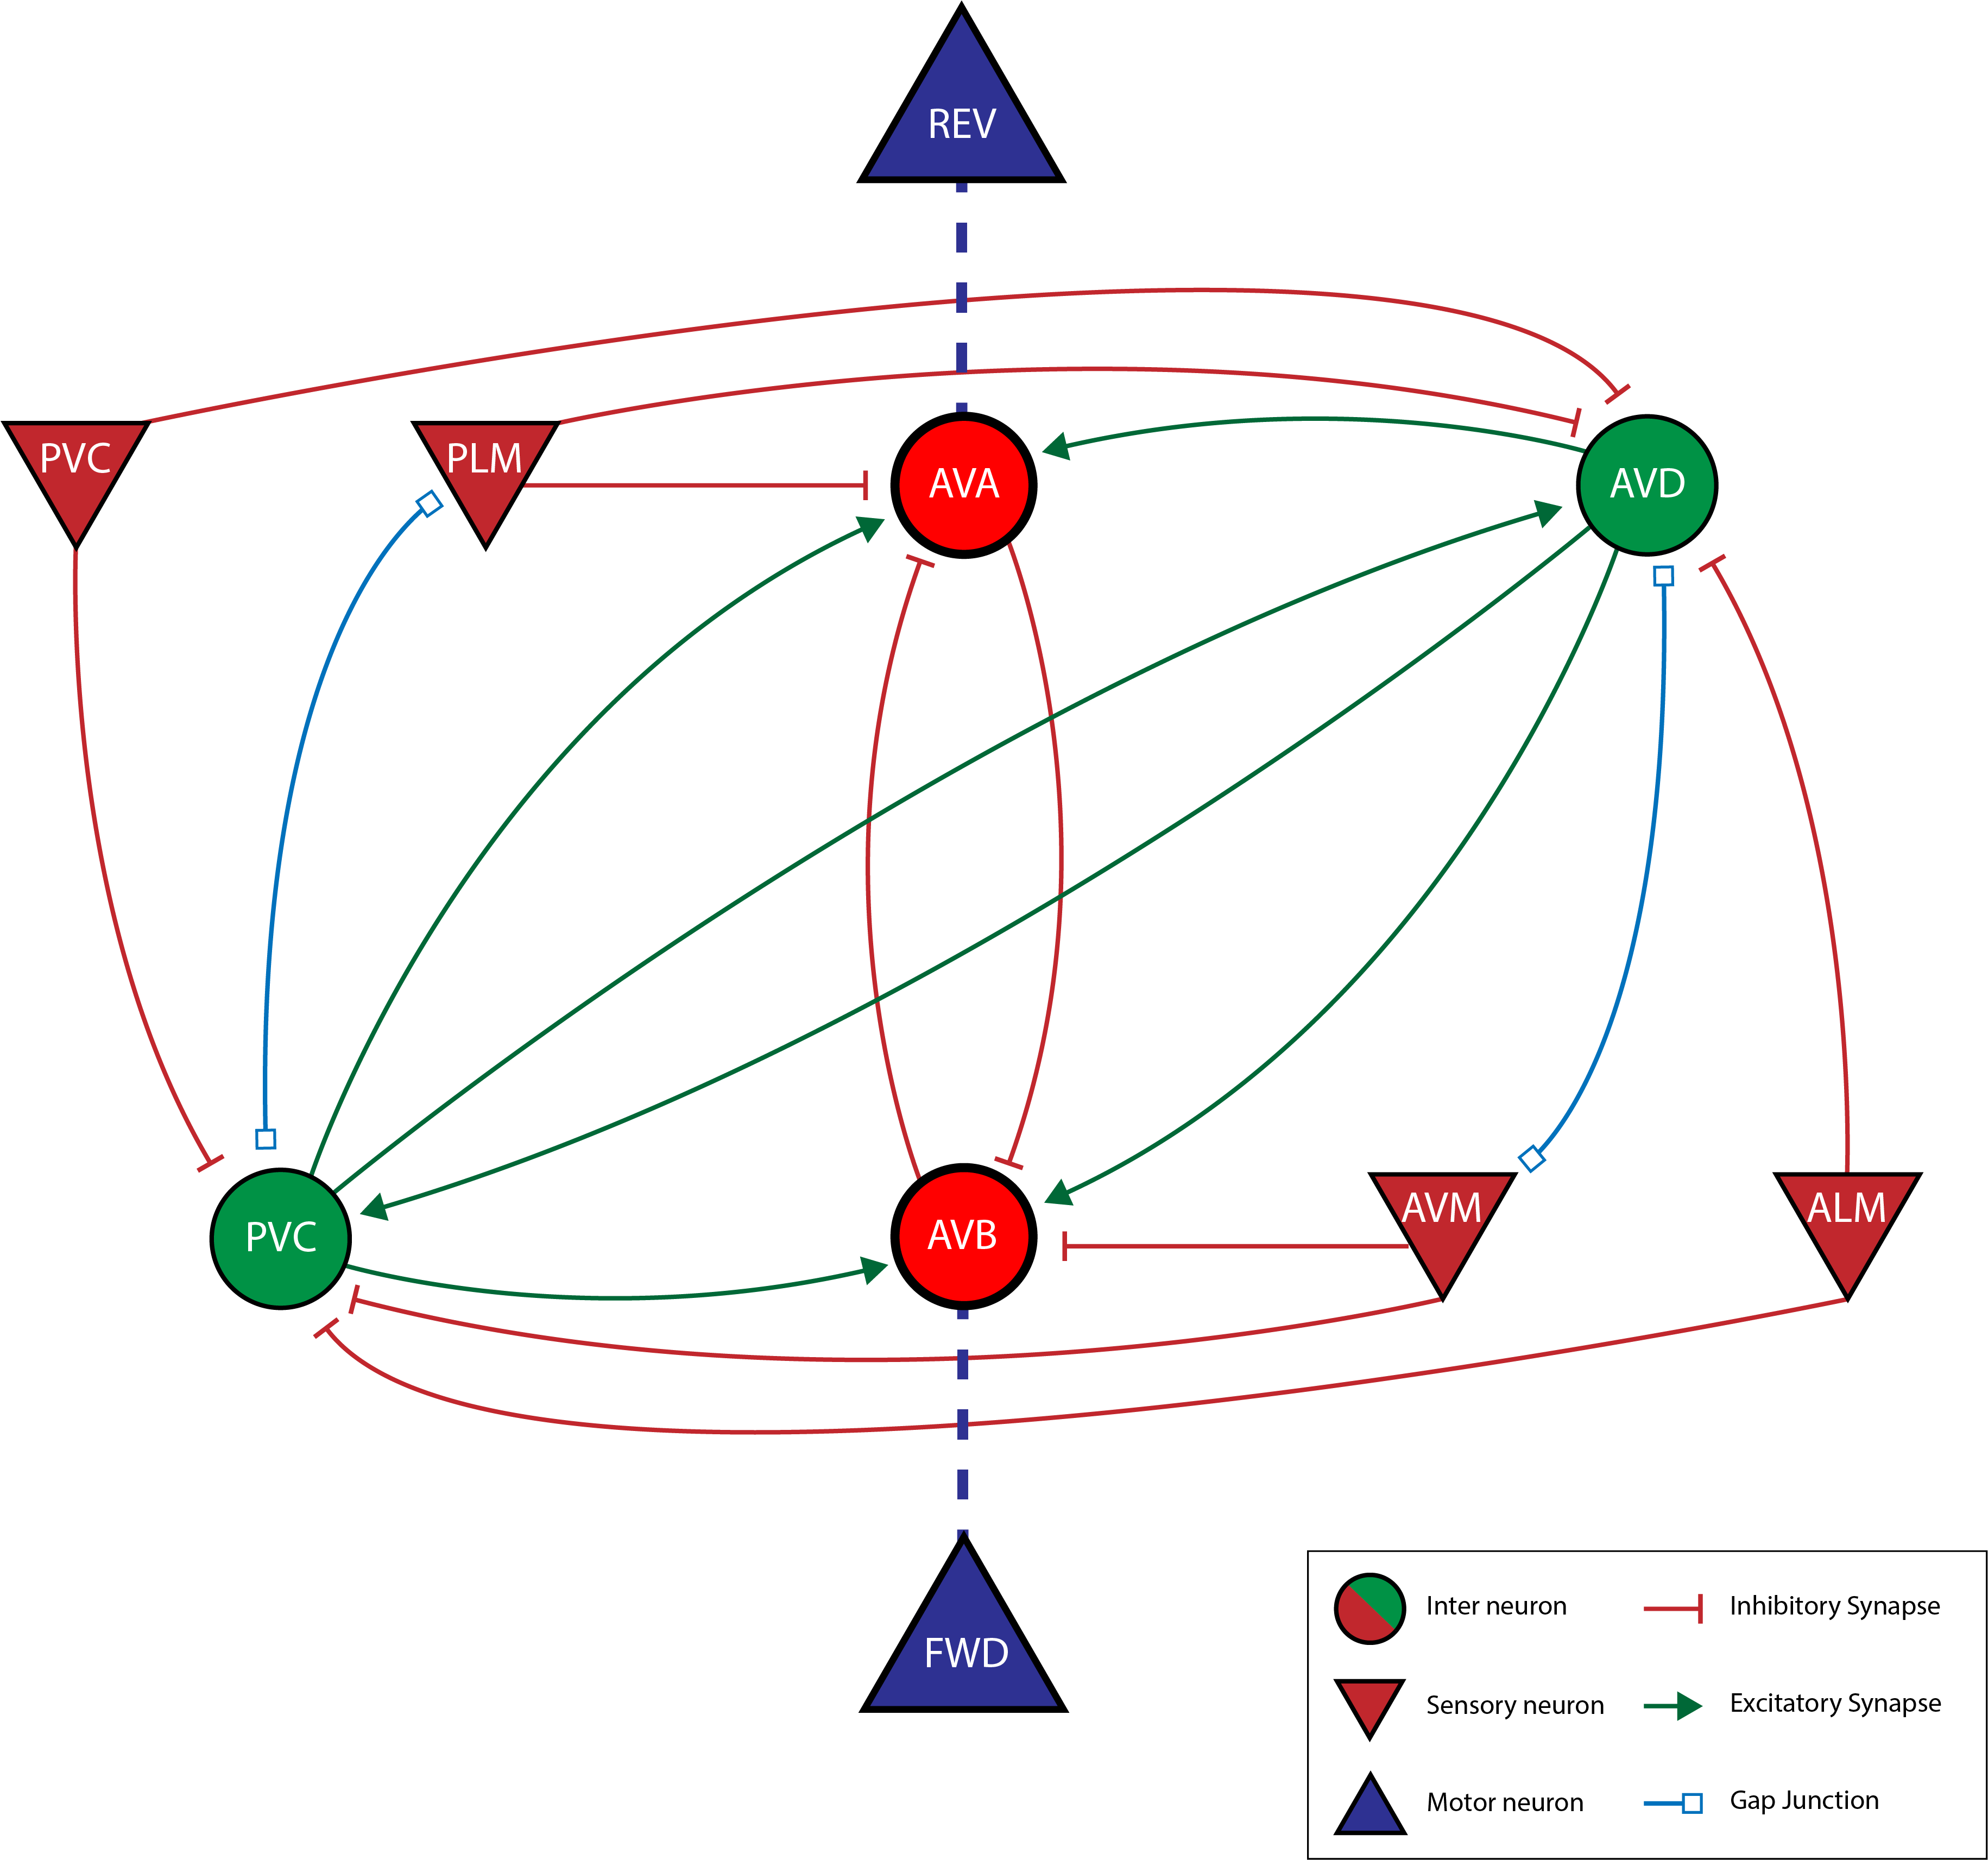
\includegraphics[width=6cm]{figures/Neural_Net.png}
  \end{minipage}
  

\end{frame}

% =======================

\begin{frame}
  \frametitle{Bisherige Schritte}
  \framesubtitle{Implementierung des \btEmph{Neuronalen Netzes mit symmetrischen Komponenten}}
  
  \textbf{Feste Parameter} - Simulation der CartPole-Environment\\
  \vspace{1cm}
  
  \begin{figure}[htb]
  	\centering
  	\begin{minipage}[t]{0.48\linewidth}
  		\centering
  		\scalebox{0.2}{%% Creator: Matplotlib, PGF backend
%%
%% To include the figure in your LaTeX document, write
%%   \input{<filename>.pgf}
%%
%% Make sure the required packages are loaded in your preamble
%%   \usepackage{pgf}
%%
%% Figures using additional raster images can only be included by \input if
%% they are in the same directory as the main LaTeX file. For loading figures
%% from other directories you can use the `import` package
%%   \usepackage{import}
%% and then include the figures with
%%   \import{<path to file>}{<filename>.pgf}
%%
%% Matplotlib used the following preamble
%%   \usepackage{fontspec}
%%   \setmainfont{Times New Roman}
%%   \setsansfont{Verdana}
%%   \setmonofont{Courier New}
%%
\begingroup%
\makeatletter%
\begin{pgfpicture}%
\pgfpathrectangle{\pgfpointorigin}{\pgfqpoint{15.360000in}{7.670000in}}%
\pgfusepath{use as bounding box, clip}%
\begin{pgfscope}%
\pgfsetbuttcap%
\pgfsetmiterjoin%
\definecolor{currentfill}{rgb}{1.000000,1.000000,1.000000}%
\pgfsetfillcolor{currentfill}%
\pgfsetlinewidth{0.000000pt}%
\definecolor{currentstroke}{rgb}{1.000000,1.000000,1.000000}%
\pgfsetstrokecolor{currentstroke}%
\pgfsetdash{}{0pt}%
\pgfpathmoveto{\pgfqpoint{0.000000in}{0.000000in}}%
\pgfpathlineto{\pgfqpoint{15.360000in}{0.000000in}}%
\pgfpathlineto{\pgfqpoint{15.360000in}{7.670000in}}%
\pgfpathlineto{\pgfqpoint{0.000000in}{7.670000in}}%
\pgfpathclose%
\pgfusepath{fill}%
\end{pgfscope}%
\begin{pgfscope}%
\pgfsetbuttcap%
\pgfsetmiterjoin%
\definecolor{currentfill}{rgb}{1.000000,1.000000,1.000000}%
\pgfsetfillcolor{currentfill}%
\pgfsetlinewidth{0.000000pt}%
\definecolor{currentstroke}{rgb}{0.000000,0.000000,0.000000}%
\pgfsetstrokecolor{currentstroke}%
\pgfsetstrokeopacity{0.000000}%
\pgfsetdash{}{0pt}%
\pgfpathmoveto{\pgfqpoint{1.920000in}{0.843700in}}%
\pgfpathlineto{\pgfqpoint{7.330909in}{0.843700in}}%
\pgfpathlineto{\pgfqpoint{7.330909in}{6.749600in}}%
\pgfpathlineto{\pgfqpoint{1.920000in}{6.749600in}}%
\pgfpathclose%
\pgfusepath{fill}%
\end{pgfscope}%
\begin{pgfscope}%
\pgfsetbuttcap%
\pgfsetroundjoin%
\definecolor{currentfill}{rgb}{0.000000,0.000000,0.000000}%
\pgfsetfillcolor{currentfill}%
\pgfsetlinewidth{0.803000pt}%
\definecolor{currentstroke}{rgb}{0.000000,0.000000,0.000000}%
\pgfsetstrokecolor{currentstroke}%
\pgfsetdash{}{0pt}%
\pgfsys@defobject{currentmarker}{\pgfqpoint{0.000000in}{-0.048611in}}{\pgfqpoint{0.000000in}{0.000000in}}{%
\pgfpathmoveto{\pgfqpoint{0.000000in}{0.000000in}}%
\pgfpathlineto{\pgfqpoint{0.000000in}{-0.048611in}}%
\pgfusepath{stroke,fill}%
}%
\begin{pgfscope}%
\pgfsys@transformshift{2.165950in}{0.843700in}%
\pgfsys@useobject{currentmarker}{}%
\end{pgfscope}%
\end{pgfscope}%
\begin{pgfscope}%
\pgftext[x=2.165950in,y=0.746478in,,top]{\sffamily\fontsize{10.000000}{12.000000}\selectfont 0}%
\end{pgfscope}%
\begin{pgfscope}%
\pgfsetbuttcap%
\pgfsetroundjoin%
\definecolor{currentfill}{rgb}{0.000000,0.000000,0.000000}%
\pgfsetfillcolor{currentfill}%
\pgfsetlinewidth{0.803000pt}%
\definecolor{currentstroke}{rgb}{0.000000,0.000000,0.000000}%
\pgfsetstrokecolor{currentstroke}%
\pgfsetdash{}{0pt}%
\pgfsys@defobject{currentmarker}{\pgfqpoint{0.000000in}{-0.048611in}}{\pgfqpoint{0.000000in}{0.000000in}}{%
\pgfpathmoveto{\pgfqpoint{0.000000in}{0.000000in}}%
\pgfpathlineto{\pgfqpoint{0.000000in}{-0.048611in}}%
\pgfusepath{stroke,fill}%
}%
\begin{pgfscope}%
\pgfsys@transformshift{3.151724in}{0.843700in}%
\pgfsys@useobject{currentmarker}{}%
\end{pgfscope}%
\end{pgfscope}%
\begin{pgfscope}%
\pgftext[x=3.151724in,y=0.746478in,,top]{\sffamily\fontsize{10.000000}{12.000000}\selectfont 100}%
\end{pgfscope}%
\begin{pgfscope}%
\pgfsetbuttcap%
\pgfsetroundjoin%
\definecolor{currentfill}{rgb}{0.000000,0.000000,0.000000}%
\pgfsetfillcolor{currentfill}%
\pgfsetlinewidth{0.803000pt}%
\definecolor{currentstroke}{rgb}{0.000000,0.000000,0.000000}%
\pgfsetstrokecolor{currentstroke}%
\pgfsetdash{}{0pt}%
\pgfsys@defobject{currentmarker}{\pgfqpoint{0.000000in}{-0.048611in}}{\pgfqpoint{0.000000in}{0.000000in}}{%
\pgfpathmoveto{\pgfqpoint{0.000000in}{0.000000in}}%
\pgfpathlineto{\pgfqpoint{0.000000in}{-0.048611in}}%
\pgfusepath{stroke,fill}%
}%
\begin{pgfscope}%
\pgfsys@transformshift{4.137497in}{0.843700in}%
\pgfsys@useobject{currentmarker}{}%
\end{pgfscope}%
\end{pgfscope}%
\begin{pgfscope}%
\pgftext[x=4.137497in,y=0.746478in,,top]{\sffamily\fontsize{10.000000}{12.000000}\selectfont 200}%
\end{pgfscope}%
\begin{pgfscope}%
\pgfsetbuttcap%
\pgfsetroundjoin%
\definecolor{currentfill}{rgb}{0.000000,0.000000,0.000000}%
\pgfsetfillcolor{currentfill}%
\pgfsetlinewidth{0.803000pt}%
\definecolor{currentstroke}{rgb}{0.000000,0.000000,0.000000}%
\pgfsetstrokecolor{currentstroke}%
\pgfsetdash{}{0pt}%
\pgfsys@defobject{currentmarker}{\pgfqpoint{0.000000in}{-0.048611in}}{\pgfqpoint{0.000000in}{0.000000in}}{%
\pgfpathmoveto{\pgfqpoint{0.000000in}{0.000000in}}%
\pgfpathlineto{\pgfqpoint{0.000000in}{-0.048611in}}%
\pgfusepath{stroke,fill}%
}%
\begin{pgfscope}%
\pgfsys@transformshift{5.123270in}{0.843700in}%
\pgfsys@useobject{currentmarker}{}%
\end{pgfscope}%
\end{pgfscope}%
\begin{pgfscope}%
\pgftext[x=5.123270in,y=0.746478in,,top]{\sffamily\fontsize{10.000000}{12.000000}\selectfont 300}%
\end{pgfscope}%
\begin{pgfscope}%
\pgfsetbuttcap%
\pgfsetroundjoin%
\definecolor{currentfill}{rgb}{0.000000,0.000000,0.000000}%
\pgfsetfillcolor{currentfill}%
\pgfsetlinewidth{0.803000pt}%
\definecolor{currentstroke}{rgb}{0.000000,0.000000,0.000000}%
\pgfsetstrokecolor{currentstroke}%
\pgfsetdash{}{0pt}%
\pgfsys@defobject{currentmarker}{\pgfqpoint{0.000000in}{-0.048611in}}{\pgfqpoint{0.000000in}{0.000000in}}{%
\pgfpathmoveto{\pgfqpoint{0.000000in}{0.000000in}}%
\pgfpathlineto{\pgfqpoint{0.000000in}{-0.048611in}}%
\pgfusepath{stroke,fill}%
}%
\begin{pgfscope}%
\pgfsys@transformshift{6.109043in}{0.843700in}%
\pgfsys@useobject{currentmarker}{}%
\end{pgfscope}%
\end{pgfscope}%
\begin{pgfscope}%
\pgftext[x=6.109043in,y=0.746478in,,top]{\sffamily\fontsize{10.000000}{12.000000}\selectfont 400}%
\end{pgfscope}%
\begin{pgfscope}%
\pgfsetbuttcap%
\pgfsetroundjoin%
\definecolor{currentfill}{rgb}{0.000000,0.000000,0.000000}%
\pgfsetfillcolor{currentfill}%
\pgfsetlinewidth{0.803000pt}%
\definecolor{currentstroke}{rgb}{0.000000,0.000000,0.000000}%
\pgfsetstrokecolor{currentstroke}%
\pgfsetdash{}{0pt}%
\pgfsys@defobject{currentmarker}{\pgfqpoint{0.000000in}{-0.048611in}}{\pgfqpoint{0.000000in}{0.000000in}}{%
\pgfpathmoveto{\pgfqpoint{0.000000in}{0.000000in}}%
\pgfpathlineto{\pgfqpoint{0.000000in}{-0.048611in}}%
\pgfusepath{stroke,fill}%
}%
\begin{pgfscope}%
\pgfsys@transformshift{7.094816in}{0.843700in}%
\pgfsys@useobject{currentmarker}{}%
\end{pgfscope}%
\end{pgfscope}%
\begin{pgfscope}%
\pgftext[x=7.094816in,y=0.746478in,,top]{\sffamily\fontsize{10.000000}{12.000000}\selectfont 500}%
\end{pgfscope}%
\begin{pgfscope}%
\pgftext[x=4.625455in,y=0.557459in,,top]{\sffamily\fontsize{10.000000}{12.000000}\selectfont t (in s)}%
\end{pgfscope}%
\begin{pgfscope}%
\pgfsetbuttcap%
\pgfsetroundjoin%
\definecolor{currentfill}{rgb}{0.000000,0.000000,0.000000}%
\pgfsetfillcolor{currentfill}%
\pgfsetlinewidth{0.803000pt}%
\definecolor{currentstroke}{rgb}{0.000000,0.000000,0.000000}%
\pgfsetstrokecolor{currentstroke}%
\pgfsetdash{}{0pt}%
\pgfsys@defobject{currentmarker}{\pgfqpoint{-0.048611in}{0.000000in}}{\pgfqpoint{0.000000in}{0.000000in}}{%
\pgfpathmoveto{\pgfqpoint{0.000000in}{0.000000in}}%
\pgfpathlineto{\pgfqpoint{-0.048611in}{0.000000in}}%
\pgfusepath{stroke,fill}%
}%
\begin{pgfscope}%
\pgfsys@transformshift{1.920000in}{1.147591in}%
\pgfsys@useobject{currentmarker}{}%
\end{pgfscope}%
\end{pgfscope}%
\begin{pgfscope}%
\pgftext[x=1.532522in,y=1.094830in,left,base]{\sffamily\fontsize{10.000000}{12.000000}\selectfont −80}%
\end{pgfscope}%
\begin{pgfscope}%
\pgfsetbuttcap%
\pgfsetroundjoin%
\definecolor{currentfill}{rgb}{0.000000,0.000000,0.000000}%
\pgfsetfillcolor{currentfill}%
\pgfsetlinewidth{0.803000pt}%
\definecolor{currentstroke}{rgb}{0.000000,0.000000,0.000000}%
\pgfsetstrokecolor{currentstroke}%
\pgfsetdash{}{0pt}%
\pgfsys@defobject{currentmarker}{\pgfqpoint{-0.048611in}{0.000000in}}{\pgfqpoint{0.000000in}{0.000000in}}{%
\pgfpathmoveto{\pgfqpoint{0.000000in}{0.000000in}}%
\pgfpathlineto{\pgfqpoint{-0.048611in}{0.000000in}}%
\pgfusepath{stroke,fill}%
}%
\begin{pgfscope}%
\pgfsys@transformshift{1.920000in}{1.894190in}%
\pgfsys@useobject{currentmarker}{}%
\end{pgfscope}%
\end{pgfscope}%
\begin{pgfscope}%
\pgftext[x=1.532522in,y=1.841428in,left,base]{\sffamily\fontsize{10.000000}{12.000000}\selectfont −70}%
\end{pgfscope}%
\begin{pgfscope}%
\pgfsetbuttcap%
\pgfsetroundjoin%
\definecolor{currentfill}{rgb}{0.000000,0.000000,0.000000}%
\pgfsetfillcolor{currentfill}%
\pgfsetlinewidth{0.803000pt}%
\definecolor{currentstroke}{rgb}{0.000000,0.000000,0.000000}%
\pgfsetstrokecolor{currentstroke}%
\pgfsetdash{}{0pt}%
\pgfsys@defobject{currentmarker}{\pgfqpoint{-0.048611in}{0.000000in}}{\pgfqpoint{0.000000in}{0.000000in}}{%
\pgfpathmoveto{\pgfqpoint{0.000000in}{0.000000in}}%
\pgfpathlineto{\pgfqpoint{-0.048611in}{0.000000in}}%
\pgfusepath{stroke,fill}%
}%
\begin{pgfscope}%
\pgfsys@transformshift{1.920000in}{2.640788in}%
\pgfsys@useobject{currentmarker}{}%
\end{pgfscope}%
\end{pgfscope}%
\begin{pgfscope}%
\pgftext[x=1.532522in,y=2.588027in,left,base]{\sffamily\fontsize{10.000000}{12.000000}\selectfont −60}%
\end{pgfscope}%
\begin{pgfscope}%
\pgfsetbuttcap%
\pgfsetroundjoin%
\definecolor{currentfill}{rgb}{0.000000,0.000000,0.000000}%
\pgfsetfillcolor{currentfill}%
\pgfsetlinewidth{0.803000pt}%
\definecolor{currentstroke}{rgb}{0.000000,0.000000,0.000000}%
\pgfsetstrokecolor{currentstroke}%
\pgfsetdash{}{0pt}%
\pgfsys@defobject{currentmarker}{\pgfqpoint{-0.048611in}{0.000000in}}{\pgfqpoint{0.000000in}{0.000000in}}{%
\pgfpathmoveto{\pgfqpoint{0.000000in}{0.000000in}}%
\pgfpathlineto{\pgfqpoint{-0.048611in}{0.000000in}}%
\pgfusepath{stroke,fill}%
}%
\begin{pgfscope}%
\pgfsys@transformshift{1.920000in}{3.387387in}%
\pgfsys@useobject{currentmarker}{}%
\end{pgfscope}%
\end{pgfscope}%
\begin{pgfscope}%
\pgftext[x=1.532522in,y=3.334625in,left,base]{\sffamily\fontsize{10.000000}{12.000000}\selectfont −50}%
\end{pgfscope}%
\begin{pgfscope}%
\pgfsetbuttcap%
\pgfsetroundjoin%
\definecolor{currentfill}{rgb}{0.000000,0.000000,0.000000}%
\pgfsetfillcolor{currentfill}%
\pgfsetlinewidth{0.803000pt}%
\definecolor{currentstroke}{rgb}{0.000000,0.000000,0.000000}%
\pgfsetstrokecolor{currentstroke}%
\pgfsetdash{}{0pt}%
\pgfsys@defobject{currentmarker}{\pgfqpoint{-0.048611in}{0.000000in}}{\pgfqpoint{0.000000in}{0.000000in}}{%
\pgfpathmoveto{\pgfqpoint{0.000000in}{0.000000in}}%
\pgfpathlineto{\pgfqpoint{-0.048611in}{0.000000in}}%
\pgfusepath{stroke,fill}%
}%
\begin{pgfscope}%
\pgfsys@transformshift{1.920000in}{4.133985in}%
\pgfsys@useobject{currentmarker}{}%
\end{pgfscope}%
\end{pgfscope}%
\begin{pgfscope}%
\pgftext[x=1.532522in,y=4.081224in,left,base]{\sffamily\fontsize{10.000000}{12.000000}\selectfont −40}%
\end{pgfscope}%
\begin{pgfscope}%
\pgfsetbuttcap%
\pgfsetroundjoin%
\definecolor{currentfill}{rgb}{0.000000,0.000000,0.000000}%
\pgfsetfillcolor{currentfill}%
\pgfsetlinewidth{0.803000pt}%
\definecolor{currentstroke}{rgb}{0.000000,0.000000,0.000000}%
\pgfsetstrokecolor{currentstroke}%
\pgfsetdash{}{0pt}%
\pgfsys@defobject{currentmarker}{\pgfqpoint{-0.048611in}{0.000000in}}{\pgfqpoint{0.000000in}{0.000000in}}{%
\pgfpathmoveto{\pgfqpoint{0.000000in}{0.000000in}}%
\pgfpathlineto{\pgfqpoint{-0.048611in}{0.000000in}}%
\pgfusepath{stroke,fill}%
}%
\begin{pgfscope}%
\pgfsys@transformshift{1.920000in}{4.880584in}%
\pgfsys@useobject{currentmarker}{}%
\end{pgfscope}%
\end{pgfscope}%
\begin{pgfscope}%
\pgftext[x=1.532522in,y=4.827822in,left,base]{\sffamily\fontsize{10.000000}{12.000000}\selectfont −30}%
\end{pgfscope}%
\begin{pgfscope}%
\pgfsetbuttcap%
\pgfsetroundjoin%
\definecolor{currentfill}{rgb}{0.000000,0.000000,0.000000}%
\pgfsetfillcolor{currentfill}%
\pgfsetlinewidth{0.803000pt}%
\definecolor{currentstroke}{rgb}{0.000000,0.000000,0.000000}%
\pgfsetstrokecolor{currentstroke}%
\pgfsetdash{}{0pt}%
\pgfsys@defobject{currentmarker}{\pgfqpoint{-0.048611in}{0.000000in}}{\pgfqpoint{0.000000in}{0.000000in}}{%
\pgfpathmoveto{\pgfqpoint{0.000000in}{0.000000in}}%
\pgfpathlineto{\pgfqpoint{-0.048611in}{0.000000in}}%
\pgfusepath{stroke,fill}%
}%
\begin{pgfscope}%
\pgfsys@transformshift{1.920000in}{5.627182in}%
\pgfsys@useobject{currentmarker}{}%
\end{pgfscope}%
\end{pgfscope}%
\begin{pgfscope}%
\pgftext[x=1.532522in,y=5.574420in,left,base]{\sffamily\fontsize{10.000000}{12.000000}\selectfont −20}%
\end{pgfscope}%
\begin{pgfscope}%
\pgfsetbuttcap%
\pgfsetroundjoin%
\definecolor{currentfill}{rgb}{0.000000,0.000000,0.000000}%
\pgfsetfillcolor{currentfill}%
\pgfsetlinewidth{0.803000pt}%
\definecolor{currentstroke}{rgb}{0.000000,0.000000,0.000000}%
\pgfsetstrokecolor{currentstroke}%
\pgfsetdash{}{0pt}%
\pgfsys@defobject{currentmarker}{\pgfqpoint{-0.048611in}{0.000000in}}{\pgfqpoint{0.000000in}{0.000000in}}{%
\pgfpathmoveto{\pgfqpoint{0.000000in}{0.000000in}}%
\pgfpathlineto{\pgfqpoint{-0.048611in}{0.000000in}}%
\pgfusepath{stroke,fill}%
}%
\begin{pgfscope}%
\pgfsys@transformshift{1.920000in}{6.373780in}%
\pgfsys@useobject{currentmarker}{}%
\end{pgfscope}%
\end{pgfscope}%
\begin{pgfscope}%
\pgftext[x=1.532522in,y=6.321019in,left,base]{\sffamily\fontsize{10.000000}{12.000000}\selectfont −10}%
\end{pgfscope}%
\begin{pgfscope}%
\pgftext[x=1.476966in,y=3.796650in,,bottom,rotate=90.000000]{\sffamily\fontsize{10.000000}{12.000000}\selectfont u(t) in [mV]}%
\end{pgfscope}%
\begin{pgfscope}%
\pgfpathrectangle{\pgfqpoint{1.920000in}{0.843700in}}{\pgfqpoint{5.410909in}{5.905900in}}%
\pgfusepath{clip}%
\pgfsetrectcap%
\pgfsetroundjoin%
\pgfsetlinewidth{1.003750pt}%
\definecolor{currentstroke}{rgb}{0.000000,0.000000,1.000000}%
\pgfsetstrokecolor{currentstroke}%
\pgfsetdash{}{0pt}%
\pgfpathmoveto{\pgfqpoint{2.165950in}{1.894190in}}%
\pgfpathlineto{\pgfqpoint{2.175808in}{1.852653in}}%
\pgfpathlineto{\pgfqpoint{2.185666in}{1.846648in}}%
\pgfpathlineto{\pgfqpoint{2.195524in}{1.834572in}}%
\pgfpathlineto{\pgfqpoint{2.205381in}{1.816421in}}%
\pgfpathlineto{\pgfqpoint{2.215239in}{1.792192in}}%
\pgfpathlineto{\pgfqpoint{2.225097in}{1.761876in}}%
\pgfpathlineto{\pgfqpoint{2.234955in}{1.725468in}}%
\pgfpathlineto{\pgfqpoint{2.244812in}{1.682962in}}%
\pgfpathlineto{\pgfqpoint{2.254670in}{1.634354in}}%
\pgfpathlineto{\pgfqpoint{2.264528in}{1.827810in}}%
\pgfpathlineto{\pgfqpoint{2.274385in}{1.822856in}}%
\pgfpathlineto{\pgfqpoint{2.284243in}{1.811821in}}%
\pgfpathlineto{\pgfqpoint{2.294101in}{1.794701in}}%
\pgfpathlineto{\pgfqpoint{2.303959in}{1.771493in}}%
\pgfpathlineto{\pgfqpoint{2.313816in}{1.742192in}}%
\pgfpathlineto{\pgfqpoint{2.323674in}{1.706790in}}%
\pgfpathlineto{\pgfqpoint{2.333532in}{1.665284in}}%
\pgfpathlineto{\pgfqpoint{2.343390in}{1.617674in}}%
\pgfpathlineto{\pgfqpoint{2.353247in}{1.894190in}}%
\pgfpathlineto{\pgfqpoint{2.392678in}{1.894190in}}%
\pgfpathlineto{\pgfqpoint{2.402536in}{1.882714in}}%
\pgfpathlineto{\pgfqpoint{2.412394in}{1.847290in}}%
\pgfpathlineto{\pgfqpoint{2.422251in}{1.805770in}}%
\pgfpathlineto{\pgfqpoint{2.432109in}{1.758151in}}%
\pgfpathlineto{\pgfqpoint{2.441967in}{1.874860in}}%
\pgfpathlineto{\pgfqpoint{2.451825in}{1.867332in}}%
\pgfpathlineto{\pgfqpoint{2.461682in}{1.853749in}}%
\pgfpathlineto{\pgfqpoint{2.471540in}{1.834110in}}%
\pgfpathlineto{\pgfqpoint{2.481398in}{1.808408in}}%
\pgfpathlineto{\pgfqpoint{2.491256in}{1.776638in}}%
\pgfpathlineto{\pgfqpoint{2.501113in}{1.738790in}}%
\pgfpathlineto{\pgfqpoint{2.510971in}{1.694857in}}%
\pgfpathlineto{\pgfqpoint{2.520829in}{1.644830in}}%
\pgfpathlineto{\pgfqpoint{2.530686in}{1.588706in}}%
\pgfpathlineto{\pgfqpoint{2.540544in}{1.854325in}}%
\pgfpathlineto{\pgfqpoint{2.550402in}{1.847298in}}%
\pgfpathlineto{\pgfqpoint{2.560260in}{1.834182in}}%
\pgfpathlineto{\pgfqpoint{2.570117in}{1.814977in}}%
\pgfpathlineto{\pgfqpoint{2.579975in}{1.789678in}}%
\pgfpathlineto{\pgfqpoint{2.589833in}{1.758280in}}%
\pgfpathlineto{\pgfqpoint{2.599691in}{1.720778in}}%
\pgfpathlineto{\pgfqpoint{2.609548in}{1.677170in}}%
\pgfpathlineto{\pgfqpoint{2.619406in}{1.894190in}}%
\pgfpathlineto{\pgfqpoint{2.629264in}{1.894190in}}%
\pgfpathlineto{\pgfqpoint{2.639122in}{1.886976in}}%
\pgfpathlineto{\pgfqpoint{2.648979in}{1.869475in}}%
\pgfpathlineto{\pgfqpoint{2.658837in}{1.845911in}}%
\pgfpathlineto{\pgfqpoint{2.668695in}{1.816276in}}%
\pgfpathlineto{\pgfqpoint{2.678552in}{1.780563in}}%
\pgfpathlineto{\pgfqpoint{2.688410in}{1.738763in}}%
\pgfpathlineto{\pgfqpoint{2.698268in}{1.690869in}}%
\pgfpathlineto{\pgfqpoint{2.708126in}{1.636877in}}%
\pgfpathlineto{\pgfqpoint{2.717983in}{1.860670in}}%
\pgfpathlineto{\pgfqpoint{2.727841in}{1.853249in}}%
\pgfpathlineto{\pgfqpoint{2.737699in}{1.839773in}}%
\pgfpathlineto{\pgfqpoint{2.747557in}{1.820241in}}%
\pgfpathlineto{\pgfqpoint{2.757414in}{1.794647in}}%
\pgfpathlineto{\pgfqpoint{2.767272in}{1.762983in}}%
\pgfpathlineto{\pgfqpoint{2.777130in}{1.725242in}}%
\pgfpathlineto{\pgfqpoint{2.786988in}{1.681415in}}%
\pgfpathlineto{\pgfqpoint{2.796845in}{1.631495in}}%
\pgfpathlineto{\pgfqpoint{2.806703in}{1.575477in}}%
\pgfpathlineto{\pgfqpoint{2.816561in}{1.894190in}}%
\pgfpathlineto{\pgfqpoint{2.846134in}{1.894190in}}%
\pgfpathlineto{\pgfqpoint{2.855992in}{1.883626in}}%
\pgfpathlineto{\pgfqpoint{2.865849in}{1.852776in}}%
\pgfpathlineto{\pgfqpoint{2.875707in}{1.815832in}}%
\pgfpathlineto{\pgfqpoint{2.885565in}{1.772789in}}%
\pgfpathlineto{\pgfqpoint{2.895423in}{1.723643in}}%
\pgfpathlineto{\pgfqpoint{2.905280in}{1.894190in}}%
\pgfpathlineto{\pgfqpoint{2.924996in}{1.894190in}}%
\pgfpathlineto{\pgfqpoint{2.934854in}{1.875851in}}%
\pgfpathlineto{\pgfqpoint{2.944711in}{1.850039in}}%
\pgfpathlineto{\pgfqpoint{2.954569in}{1.818128in}}%
\pgfpathlineto{\pgfqpoint{2.964427in}{1.780111in}}%
\pgfpathlineto{\pgfqpoint{2.974284in}{1.735987in}}%
\pgfpathlineto{\pgfqpoint{2.984142in}{1.827183in}}%
\pgfpathlineto{\pgfqpoint{2.994000in}{1.822611in}}%
\pgfpathlineto{\pgfqpoint{3.003858in}{1.811971in}}%
\pgfpathlineto{\pgfqpoint{3.013715in}{1.795262in}}%
\pgfpathlineto{\pgfqpoint{3.023573in}{1.772479in}}%
\pgfpathlineto{\pgfqpoint{3.033431in}{1.743615in}}%
\pgfpathlineto{\pgfqpoint{3.043289in}{1.708663in}}%
\pgfpathlineto{\pgfqpoint{3.053146in}{1.667616in}}%
\pgfpathlineto{\pgfqpoint{3.063004in}{1.620470in}}%
\pgfpathlineto{\pgfqpoint{3.072862in}{1.567222in}}%
\pgfpathlineto{\pgfqpoint{3.082719in}{1.826928in}}%
\pgfpathlineto{\pgfqpoint{3.092577in}{1.820631in}}%
\pgfpathlineto{\pgfqpoint{3.102435in}{1.808254in}}%
\pgfpathlineto{\pgfqpoint{3.112293in}{1.789796in}}%
\pgfpathlineto{\pgfqpoint{3.122150in}{1.765252in}}%
\pgfpathlineto{\pgfqpoint{3.132008in}{1.734616in}}%
\pgfpathlineto{\pgfqpoint{3.141866in}{1.697883in}}%
\pgfpathlineto{\pgfqpoint{3.151724in}{1.655047in}}%
\pgfpathlineto{\pgfqpoint{3.161581in}{1.606106in}}%
\pgfpathlineto{\pgfqpoint{3.171439in}{1.894190in}}%
\pgfpathlineto{\pgfqpoint{3.191155in}{1.894190in}}%
\pgfpathlineto{\pgfqpoint{3.201012in}{1.887347in}}%
\pgfpathlineto{\pgfqpoint{3.210870in}{1.864557in}}%
\pgfpathlineto{\pgfqpoint{3.220728in}{1.835679in}}%
\pgfpathlineto{\pgfqpoint{3.230585in}{1.800709in}}%
\pgfpathlineto{\pgfqpoint{3.240443in}{1.759639in}}%
\pgfpathlineto{\pgfqpoint{3.250301in}{1.712466in}}%
\pgfpathlineto{\pgfqpoint{3.260159in}{1.870102in}}%
\pgfpathlineto{\pgfqpoint{3.270016in}{1.863901in}}%
\pgfpathlineto{\pgfqpoint{3.279874in}{1.851626in}}%
\pgfpathlineto{\pgfqpoint{3.289732in}{1.833273in}}%
\pgfpathlineto{\pgfqpoint{3.299590in}{1.808838in}}%
\pgfpathlineto{\pgfqpoint{3.309447in}{1.778316in}}%
\pgfpathlineto{\pgfqpoint{3.319305in}{1.741699in}}%
\pgfpathlineto{\pgfqpoint{3.329163in}{1.698982in}}%
\pgfpathlineto{\pgfqpoint{3.339021in}{1.650162in}}%
\pgfpathlineto{\pgfqpoint{3.348878in}{1.894190in}}%
\pgfpathlineto{\pgfqpoint{3.378451in}{1.894190in}}%
\pgfpathlineto{\pgfqpoint{3.388309in}{1.879274in}}%
\pgfpathlineto{\pgfqpoint{3.398167in}{1.848938in}}%
\pgfpathlineto{\pgfqpoint{3.408025in}{1.812520in}}%
\pgfpathlineto{\pgfqpoint{3.417882in}{1.770012in}}%
\pgfpathlineto{\pgfqpoint{3.427740in}{1.721407in}}%
\pgfpathlineto{\pgfqpoint{3.437598in}{1.666704in}}%
\pgfpathlineto{\pgfqpoint{3.447456in}{1.894190in}}%
\pgfpathlineto{\pgfqpoint{3.477029in}{1.894190in}}%
\pgfpathlineto{\pgfqpoint{3.486887in}{1.885741in}}%
\pgfpathlineto{\pgfqpoint{3.496744in}{1.855663in}}%
\pgfpathlineto{\pgfqpoint{3.506602in}{1.819486in}}%
\pgfpathlineto{\pgfqpoint{3.516460in}{1.777204in}}%
\pgfpathlineto{\pgfqpoint{3.526317in}{1.728817in}}%
\pgfpathlineto{\pgfqpoint{3.536175in}{1.894190in}}%
\pgfpathlineto{\pgfqpoint{3.565748in}{1.894190in}}%
\pgfpathlineto{\pgfqpoint{3.575606in}{1.875001in}}%
\pgfpathlineto{\pgfqpoint{3.585464in}{1.844794in}}%
\pgfpathlineto{\pgfqpoint{3.595322in}{1.808485in}}%
\pgfpathlineto{\pgfqpoint{3.605179in}{1.766073in}}%
\pgfpathlineto{\pgfqpoint{3.615037in}{1.717554in}}%
\pgfpathlineto{\pgfqpoint{3.624895in}{1.828204in}}%
\pgfpathlineto{\pgfqpoint{3.634752in}{1.823283in}}%
\pgfpathlineto{\pgfqpoint{3.644610in}{1.812278in}}%
\pgfpathlineto{\pgfqpoint{3.654468in}{1.795188in}}%
\pgfpathlineto{\pgfqpoint{3.664326in}{1.772008in}}%
\pgfpathlineto{\pgfqpoint{3.674183in}{1.742732in}}%
\pgfpathlineto{\pgfqpoint{3.684041in}{1.707356in}}%
\pgfpathlineto{\pgfqpoint{3.693899in}{1.665875in}}%
\pgfpathlineto{\pgfqpoint{3.703757in}{1.618289in}}%
\pgfpathlineto{\pgfqpoint{3.713614in}{1.872186in}}%
\pgfpathlineto{\pgfqpoint{3.723472in}{1.866506in}}%
\pgfpathlineto{\pgfqpoint{3.733330in}{1.854746in}}%
\pgfpathlineto{\pgfqpoint{3.743188in}{1.836903in}}%
\pgfpathlineto{\pgfqpoint{3.753045in}{1.812973in}}%
\pgfpathlineto{\pgfqpoint{3.762903in}{1.782951in}}%
\pgfpathlineto{\pgfqpoint{3.772761in}{1.746829in}}%
\pgfpathlineto{\pgfqpoint{3.782618in}{1.704605in}}%
\pgfpathlineto{\pgfqpoint{3.792476in}{1.656276in}}%
\pgfpathlineto{\pgfqpoint{3.802334in}{1.894190in}}%
\pgfpathlineto{\pgfqpoint{3.831907in}{1.894190in}}%
\pgfpathlineto{\pgfqpoint{3.841765in}{1.886905in}}%
\pgfpathlineto{\pgfqpoint{3.851623in}{1.856428in}}%
\pgfpathlineto{\pgfqpoint{3.861480in}{1.819870in}}%
\pgfpathlineto{\pgfqpoint{3.871338in}{1.777224in}}%
\pgfpathlineto{\pgfqpoint{3.881196in}{1.728483in}}%
\pgfpathlineto{\pgfqpoint{3.891054in}{1.673644in}}%
\pgfpathlineto{\pgfqpoint{3.900911in}{1.847635in}}%
\pgfpathlineto{\pgfqpoint{3.910769in}{1.840518in}}%
\pgfpathlineto{\pgfqpoint{3.920627in}{1.827334in}}%
\pgfpathlineto{\pgfqpoint{3.930484in}{1.808081in}}%
\pgfpathlineto{\pgfqpoint{3.940342in}{1.782752in}}%
\pgfpathlineto{\pgfqpoint{3.950200in}{1.751342in}}%
\pgfpathlineto{\pgfqpoint{3.960058in}{1.713843in}}%
\pgfpathlineto{\pgfqpoint{3.969915in}{1.670249in}}%
\pgfpathlineto{\pgfqpoint{3.979773in}{1.620554in}}%
\pgfpathlineto{\pgfqpoint{3.989631in}{1.849309in}}%
\pgfpathlineto{\pgfqpoint{3.999489in}{1.842563in}}%
\pgfpathlineto{\pgfqpoint{4.009346in}{1.829740in}}%
\pgfpathlineto{\pgfqpoint{4.019204in}{1.810837in}}%
\pgfpathlineto{\pgfqpoint{4.029062in}{1.785851in}}%
\pgfpathlineto{\pgfqpoint{4.038919in}{1.754776in}}%
\pgfpathlineto{\pgfqpoint{4.048777in}{1.717606in}}%
\pgfpathlineto{\pgfqpoint{4.058635in}{1.674335in}}%
\pgfpathlineto{\pgfqpoint{4.068493in}{1.624960in}}%
\pgfpathlineto{\pgfqpoint{4.078350in}{1.894190in}}%
\pgfpathlineto{\pgfqpoint{4.088208in}{1.894190in}}%
\pgfpathlineto{\pgfqpoint{4.098066in}{1.893055in}}%
\pgfpathlineto{\pgfqpoint{4.107924in}{1.873803in}}%
\pgfpathlineto{\pgfqpoint{4.117781in}{1.848457in}}%
\pgfpathlineto{\pgfqpoint{4.127639in}{1.817012in}}%
\pgfpathlineto{\pgfqpoint{4.137497in}{1.779463in}}%
\pgfpathlineto{\pgfqpoint{4.147355in}{1.735807in}}%
\pgfpathlineto{\pgfqpoint{4.157212in}{1.842376in}}%
\pgfpathlineto{\pgfqpoint{4.167070in}{1.836668in}}%
\pgfpathlineto{\pgfqpoint{4.176928in}{1.824908in}}%
\pgfpathlineto{\pgfqpoint{4.186785in}{1.807094in}}%
\pgfpathlineto{\pgfqpoint{4.196643in}{1.783219in}}%
\pgfpathlineto{\pgfqpoint{4.206501in}{1.753275in}}%
\pgfpathlineto{\pgfqpoint{4.216359in}{1.717255in}}%
\pgfpathlineto{\pgfqpoint{4.226216in}{1.675148in}}%
\pgfpathlineto{\pgfqpoint{4.236074in}{1.626949in}}%
\pgfpathlineto{\pgfqpoint{4.245932in}{1.572653in}}%
\pgfpathlineto{\pgfqpoint{4.255790in}{1.870600in}}%
\pgfpathlineto{\pgfqpoint{4.265647in}{1.865331in}}%
\pgfpathlineto{\pgfqpoint{4.275505in}{1.853974in}}%
\pgfpathlineto{\pgfqpoint{4.285363in}{1.836527in}}%
\pgfpathlineto{\pgfqpoint{4.295221in}{1.812985in}}%
\pgfpathlineto{\pgfqpoint{4.305078in}{1.783345in}}%
\pgfpathlineto{\pgfqpoint{4.314936in}{1.747600in}}%
\pgfpathlineto{\pgfqpoint{4.324794in}{1.705749in}}%
\pgfpathlineto{\pgfqpoint{4.334651in}{1.854908in}}%
\pgfpathlineto{\pgfqpoint{4.344509in}{1.847762in}}%
\pgfpathlineto{\pgfqpoint{4.354367in}{1.834529in}}%
\pgfpathlineto{\pgfqpoint{4.364225in}{1.815205in}}%
\pgfpathlineto{\pgfqpoint{4.374082in}{1.789787in}}%
\pgfpathlineto{\pgfqpoint{4.383940in}{1.758270in}}%
\pgfpathlineto{\pgfqpoint{4.393798in}{1.720650in}}%
\pgfpathlineto{\pgfqpoint{4.403656in}{1.676922in}}%
\pgfpathlineto{\pgfqpoint{4.413513in}{1.894190in}}%
\pgfpathlineto{\pgfqpoint{4.452944in}{1.894190in}}%
\pgfpathlineto{\pgfqpoint{4.462802in}{1.870533in}}%
\pgfpathlineto{\pgfqpoint{4.472660in}{1.833543in}}%
\pgfpathlineto{\pgfqpoint{4.482517in}{1.790447in}}%
\pgfpathlineto{\pgfqpoint{4.492375in}{1.741244in}}%
\pgfpathlineto{\pgfqpoint{4.502233in}{1.872157in}}%
\pgfpathlineto{\pgfqpoint{4.512091in}{1.864892in}}%
\pgfpathlineto{\pgfqpoint{4.521948in}{1.851575in}}%
\pgfpathlineto{\pgfqpoint{4.531806in}{1.832204in}}%
\pgfpathlineto{\pgfqpoint{4.541664in}{1.806772in}}%
\pgfpathlineto{\pgfqpoint{4.551522in}{1.775273in}}%
\pgfpathlineto{\pgfqpoint{4.561379in}{1.737697in}}%
\pgfpathlineto{\pgfqpoint{4.571237in}{1.694035in}}%
\pgfpathlineto{\pgfqpoint{4.581095in}{1.644280in}}%
\pgfpathlineto{\pgfqpoint{4.590952in}{1.588429in}}%
\pgfpathlineto{\pgfqpoint{4.600810in}{1.816808in}}%
\pgfpathlineto{\pgfqpoint{4.610668in}{1.809443in}}%
\pgfpathlineto{\pgfqpoint{4.620526in}{1.795987in}}%
\pgfpathlineto{\pgfqpoint{4.630383in}{1.776438in}}%
\pgfpathlineto{\pgfqpoint{4.640241in}{1.750792in}}%
\pgfpathlineto{\pgfqpoint{4.650099in}{1.719045in}}%
\pgfpathlineto{\pgfqpoint{4.659957in}{1.681191in}}%
\pgfpathlineto{\pgfqpoint{4.669814in}{1.637229in}}%
\pgfpathlineto{\pgfqpoint{4.679672in}{1.824504in}}%
\pgfpathlineto{\pgfqpoint{4.689530in}{1.818378in}}%
\pgfpathlineto{\pgfqpoint{4.699388in}{1.806166in}}%
\pgfpathlineto{\pgfqpoint{4.709245in}{1.787869in}}%
\pgfpathlineto{\pgfqpoint{4.719103in}{1.763480in}}%
\pgfpathlineto{\pgfqpoint{4.728961in}{1.732996in}}%
\pgfpathlineto{\pgfqpoint{4.738818in}{1.696410in}}%
\pgfpathlineto{\pgfqpoint{4.748676in}{1.653719in}}%
\pgfpathlineto{\pgfqpoint{4.758534in}{1.604921in}}%
\pgfpathlineto{\pgfqpoint{4.768392in}{1.894190in}}%
\pgfpathlineto{\pgfqpoint{4.797965in}{1.894190in}}%
\pgfpathlineto{\pgfqpoint{4.807823in}{1.877151in}}%
\pgfpathlineto{\pgfqpoint{4.817680in}{1.846802in}}%
\pgfpathlineto{\pgfqpoint{4.827538in}{1.810363in}}%
\pgfpathlineto{\pgfqpoint{4.837396in}{1.767827in}}%
\pgfpathlineto{\pgfqpoint{4.847254in}{1.719190in}}%
\pgfpathlineto{\pgfqpoint{4.857111in}{1.889495in}}%
\pgfpathlineto{\pgfqpoint{4.866969in}{1.883053in}}%
\pgfpathlineto{\pgfqpoint{4.876827in}{1.870531in}}%
\pgfpathlineto{\pgfqpoint{4.886684in}{1.851926in}}%
\pgfpathlineto{\pgfqpoint{4.896542in}{1.827235in}}%
\pgfpathlineto{\pgfqpoint{4.906400in}{1.796451in}}%
\pgfpathlineto{\pgfqpoint{4.916258in}{1.759570in}}%
\pgfpathlineto{\pgfqpoint{4.926115in}{1.716586in}}%
\pgfpathlineto{\pgfqpoint{4.935973in}{1.667497in}}%
\pgfpathlineto{\pgfqpoint{4.945831in}{1.820715in}}%
\pgfpathlineto{\pgfqpoint{4.955689in}{1.815063in}}%
\pgfpathlineto{\pgfqpoint{4.965546in}{1.803353in}}%
\pgfpathlineto{\pgfqpoint{4.975404in}{1.785582in}}%
\pgfpathlineto{\pgfqpoint{4.985262in}{1.761746in}}%
\pgfpathlineto{\pgfqpoint{4.995119in}{1.731837in}}%
\pgfpathlineto{\pgfqpoint{5.004977in}{1.695848in}}%
\pgfpathlineto{\pgfqpoint{5.014835in}{1.653769in}}%
\pgfpathlineto{\pgfqpoint{5.024693in}{1.605594in}}%
\pgfpathlineto{\pgfqpoint{5.034550in}{1.551322in}}%
\pgfpathlineto{\pgfqpoint{5.044408in}{1.826157in}}%
\pgfpathlineto{\pgfqpoint{5.054266in}{1.819711in}}%
\pgfpathlineto{\pgfqpoint{5.064124in}{1.807174in}}%
\pgfpathlineto{\pgfqpoint{5.073981in}{1.788546in}}%
\pgfpathlineto{\pgfqpoint{5.083839in}{1.763821in}}%
\pgfpathlineto{\pgfqpoint{5.093697in}{1.732996in}}%
\pgfpathlineto{\pgfqpoint{5.103555in}{1.696065in}}%
\pgfpathlineto{\pgfqpoint{5.113412in}{1.653026in}}%
\pgfpathlineto{\pgfqpoint{5.123270in}{1.894190in}}%
\pgfpathlineto{\pgfqpoint{5.162701in}{1.894190in}}%
\pgfpathlineto{\pgfqpoint{5.172559in}{1.870068in}}%
\pgfpathlineto{\pgfqpoint{5.182416in}{1.832977in}}%
\pgfpathlineto{\pgfqpoint{5.192274in}{1.789793in}}%
\pgfpathlineto{\pgfqpoint{5.202132in}{1.740510in}}%
\pgfpathlineto{\pgfqpoint{5.211990in}{1.685128in}}%
\pgfpathlineto{\pgfqpoint{5.221847in}{1.894190in}}%
\pgfpathlineto{\pgfqpoint{5.241563in}{1.894190in}}%
\pgfpathlineto{\pgfqpoint{5.251421in}{1.892191in}}%
\pgfpathlineto{\pgfqpoint{5.261278in}{1.867532in}}%
\pgfpathlineto{\pgfqpoint{5.271136in}{1.836777in}}%
\pgfpathlineto{\pgfqpoint{5.280994in}{1.799921in}}%
\pgfpathlineto{\pgfqpoint{5.290851in}{1.756960in}}%
\pgfpathlineto{\pgfqpoint{5.300709in}{1.707892in}}%
\pgfpathlineto{\pgfqpoint{5.310567in}{1.894190in}}%
\pgfpathlineto{\pgfqpoint{5.330282in}{1.894190in}}%
\pgfpathlineto{\pgfqpoint{5.340140in}{1.882975in}}%
\pgfpathlineto{\pgfqpoint{5.349998in}{1.859755in}}%
\pgfpathlineto{\pgfqpoint{5.359856in}{1.830459in}}%
\pgfpathlineto{\pgfqpoint{5.369713in}{1.795077in}}%
\pgfpathlineto{\pgfqpoint{5.379571in}{1.753604in}}%
\pgfpathlineto{\pgfqpoint{5.389429in}{1.706033in}}%
\pgfpathlineto{\pgfqpoint{5.399287in}{1.652362in}}%
\pgfpathlineto{\pgfqpoint{5.409144in}{1.868762in}}%
\pgfpathlineto{\pgfqpoint{5.419002in}{1.862837in}}%
\pgfpathlineto{\pgfqpoint{5.428860in}{1.850832in}}%
\pgfpathlineto{\pgfqpoint{5.438717in}{1.832743in}}%
\pgfpathlineto{\pgfqpoint{5.448575in}{1.808567in}}%
\pgfpathlineto{\pgfqpoint{5.458433in}{1.778297in}}%
\pgfpathlineto{\pgfqpoint{5.468291in}{1.741928in}}%
\pgfpathlineto{\pgfqpoint{5.478148in}{1.699455in}}%
\pgfpathlineto{\pgfqpoint{5.488006in}{1.650877in}}%
\pgfpathlineto{\pgfqpoint{5.497864in}{1.846614in}}%
\pgfpathlineto{\pgfqpoint{5.507722in}{1.840133in}}%
\pgfpathlineto{\pgfqpoint{5.517579in}{1.827594in}}%
\pgfpathlineto{\pgfqpoint{5.527437in}{1.808994in}}%
\pgfpathlineto{\pgfqpoint{5.537295in}{1.784328in}}%
\pgfpathlineto{\pgfqpoint{5.547152in}{1.753590in}}%
\pgfpathlineto{\pgfqpoint{5.557010in}{1.716771in}}%
\pgfpathlineto{\pgfqpoint{5.566868in}{1.673864in}}%
\pgfpathlineto{\pgfqpoint{5.576726in}{1.624862in}}%
\pgfpathlineto{\pgfqpoint{5.586583in}{1.569761in}}%
\pgfpathlineto{\pgfqpoint{5.596441in}{1.894190in}}%
\pgfpathlineto{\pgfqpoint{5.635872in}{1.894190in}}%
\pgfpathlineto{\pgfqpoint{5.645730in}{1.880211in}}%
\pgfpathlineto{\pgfqpoint{5.655588in}{1.844640in}}%
\pgfpathlineto{\pgfqpoint{5.665445in}{1.802976in}}%
\pgfpathlineto{\pgfqpoint{5.675303in}{1.755213in}}%
\pgfpathlineto{\pgfqpoint{5.685161in}{1.701350in}}%
\pgfpathlineto{\pgfqpoint{5.695018in}{1.822882in}}%
\pgfpathlineto{\pgfqpoint{5.704876in}{1.817742in}}%
\pgfpathlineto{\pgfqpoint{5.714734in}{1.806518in}}%
\pgfpathlineto{\pgfqpoint{5.724592in}{1.789207in}}%
\pgfpathlineto{\pgfqpoint{5.734449in}{1.765805in}}%
\pgfpathlineto{\pgfqpoint{5.744307in}{1.736307in}}%
\pgfpathlineto{\pgfqpoint{5.754165in}{1.700707in}}%
\pgfpathlineto{\pgfqpoint{5.764023in}{1.659002in}}%
\pgfpathlineto{\pgfqpoint{5.773880in}{1.611191in}}%
\pgfpathlineto{\pgfqpoint{5.783738in}{1.894190in}}%
\pgfpathlineto{\pgfqpoint{5.793596in}{1.894190in}}%
\pgfpathlineto{\pgfqpoint{5.803454in}{1.886816in}}%
\pgfpathlineto{\pgfqpoint{5.813311in}{1.869387in}}%
\pgfpathlineto{\pgfqpoint{5.823169in}{1.845887in}}%
\pgfpathlineto{\pgfqpoint{5.833027in}{1.816311in}}%
\pgfpathlineto{\pgfqpoint{5.842884in}{1.780649in}}%
\pgfpathlineto{\pgfqpoint{5.852742in}{1.738894in}}%
\pgfpathlineto{\pgfqpoint{5.862600in}{1.691042in}}%
\pgfpathlineto{\pgfqpoint{5.872458in}{1.637090in}}%
\pgfpathlineto{\pgfqpoint{5.882315in}{1.894190in}}%
\pgfpathlineto{\pgfqpoint{5.911889in}{1.894190in}}%
\pgfpathlineto{\pgfqpoint{5.921746in}{1.889113in}}%
\pgfpathlineto{\pgfqpoint{5.931604in}{1.858476in}}%
\pgfpathlineto{\pgfqpoint{5.941462in}{1.821743in}}%
\pgfpathlineto{\pgfqpoint{5.951319in}{1.778910in}}%
\pgfpathlineto{\pgfqpoint{5.961177in}{1.729973in}}%
\pgfpathlineto{\pgfqpoint{5.971035in}{1.894190in}}%
\pgfpathlineto{\pgfqpoint{6.010466in}{1.894190in}}%
\pgfpathlineto{\pgfqpoint{6.020324in}{1.878448in}}%
\pgfpathlineto{\pgfqpoint{6.030181in}{1.843635in}}%
\pgfpathlineto{\pgfqpoint{6.040039in}{1.802739in}}%
\pgfpathlineto{\pgfqpoint{6.049897in}{1.755753in}}%
\pgfpathlineto{\pgfqpoint{6.059755in}{1.702670in}}%
\pgfpathlineto{\pgfqpoint{6.069612in}{1.643492in}}%
\pgfpathlineto{\pgfqpoint{6.079470in}{1.894190in}}%
\pgfpathlineto{\pgfqpoint{6.099185in}{1.894109in}}%
\pgfpathlineto{\pgfqpoint{6.109043in}{1.876636in}}%
\pgfpathlineto{\pgfqpoint{6.118901in}{1.853067in}}%
\pgfpathlineto{\pgfqpoint{6.128759in}{1.823397in}}%
\pgfpathlineto{\pgfqpoint{6.138616in}{1.787622in}}%
\pgfpathlineto{\pgfqpoint{6.148474in}{1.745739in}}%
\pgfpathlineto{\pgfqpoint{6.158332in}{1.894190in}}%
\pgfpathlineto{\pgfqpoint{6.187905in}{1.894190in}}%
\pgfpathlineto{\pgfqpoint{6.197763in}{1.890486in}}%
\pgfpathlineto{\pgfqpoint{6.207621in}{1.859407in}}%
\pgfpathlineto{\pgfqpoint{6.217478in}{1.822231in}}%
\pgfpathlineto{\pgfqpoint{6.227336in}{1.778952in}}%
\pgfpathlineto{\pgfqpoint{6.237194in}{1.729569in}}%
\pgfpathlineto{\pgfqpoint{6.247051in}{1.841223in}}%
\pgfpathlineto{\pgfqpoint{6.256909in}{1.834081in}}%
\pgfpathlineto{\pgfqpoint{6.266767in}{1.820889in}}%
\pgfpathlineto{\pgfqpoint{6.276625in}{1.801647in}}%
\pgfpathlineto{\pgfqpoint{6.286482in}{1.776348in}}%
\pgfpathlineto{\pgfqpoint{6.296340in}{1.744985in}}%
\pgfpathlineto{\pgfqpoint{6.306198in}{1.707550in}}%
\pgfpathlineto{\pgfqpoint{6.316056in}{1.664032in}}%
\pgfpathlineto{\pgfqpoint{6.325913in}{1.614425in}}%
\pgfpathlineto{\pgfqpoint{6.345629in}{1.496925in}}%
\pgfpathlineto{\pgfqpoint{6.355487in}{1.894190in}}%
\pgfpathlineto{\pgfqpoint{6.385060in}{1.894190in}}%
\pgfpathlineto{\pgfqpoint{6.394917in}{1.878499in}}%
\pgfpathlineto{\pgfqpoint{6.404775in}{1.848787in}}%
\pgfpathlineto{\pgfqpoint{6.414633in}{1.812984in}}%
\pgfpathlineto{\pgfqpoint{6.424491in}{1.771084in}}%
\pgfpathlineto{\pgfqpoint{6.434348in}{1.723083in}}%
\pgfpathlineto{\pgfqpoint{6.444206in}{1.894190in}}%
\pgfpathlineto{\pgfqpoint{6.483637in}{1.894190in}}%
\pgfpathlineto{\pgfqpoint{6.493495in}{1.886300in}}%
\pgfpathlineto{\pgfqpoint{6.503352in}{1.851386in}}%
\pgfpathlineto{\pgfqpoint{6.513210in}{1.810374in}}%
\pgfpathlineto{\pgfqpoint{6.523068in}{1.763260in}}%
\pgfpathlineto{\pgfqpoint{6.532926in}{1.826494in}}%
\pgfpathlineto{\pgfqpoint{6.542783in}{1.819860in}}%
\pgfpathlineto{\pgfqpoint{6.552641in}{1.807171in}}%
\pgfpathlineto{\pgfqpoint{6.562499in}{1.788424in}}%
\pgfpathlineto{\pgfqpoint{6.572357in}{1.763614in}}%
\pgfpathlineto{\pgfqpoint{6.582214in}{1.732733in}}%
\pgfpathlineto{\pgfqpoint{6.592072in}{1.695772in}}%
\pgfpathlineto{\pgfqpoint{6.601930in}{1.652723in}}%
\pgfpathlineto{\pgfqpoint{6.611788in}{1.603579in}}%
\pgfpathlineto{\pgfqpoint{6.621645in}{1.548338in}}%
\pgfpathlineto{\pgfqpoint{6.631503in}{1.894190in}}%
\pgfpathlineto{\pgfqpoint{6.641361in}{1.890243in}}%
\pgfpathlineto{\pgfqpoint{6.651218in}{1.879258in}}%
\pgfpathlineto{\pgfqpoint{6.661076in}{1.862191in}}%
\pgfpathlineto{\pgfqpoint{6.670934in}{1.839037in}}%
\pgfpathlineto{\pgfqpoint{6.680792in}{1.809790in}}%
\pgfpathlineto{\pgfqpoint{6.690649in}{1.774446in}}%
\pgfpathlineto{\pgfqpoint{6.700507in}{1.732998in}}%
\pgfpathlineto{\pgfqpoint{6.710365in}{1.685446in}}%
\pgfpathlineto{\pgfqpoint{6.720223in}{1.894190in}}%
\pgfpathlineto{\pgfqpoint{6.730080in}{1.888560in}}%
\pgfpathlineto{\pgfqpoint{6.739938in}{1.876851in}}%
\pgfpathlineto{\pgfqpoint{6.749796in}{1.859073in}}%
\pgfpathlineto{\pgfqpoint{6.759654in}{1.835223in}}%
\pgfpathlineto{\pgfqpoint{6.769511in}{1.805293in}}%
\pgfpathlineto{\pgfqpoint{6.779369in}{1.769277in}}%
\pgfpathlineto{\pgfqpoint{6.789227in}{1.727167in}}%
\pgfpathlineto{\pgfqpoint{6.799084in}{1.678957in}}%
\pgfpathlineto{\pgfqpoint{6.808942in}{1.624648in}}%
\pgfpathlineto{\pgfqpoint{6.818800in}{1.841019in}}%
\pgfpathlineto{\pgfqpoint{6.828658in}{1.834927in}}%
\pgfpathlineto{\pgfqpoint{6.838515in}{1.822774in}}%
\pgfpathlineto{\pgfqpoint{6.848373in}{1.804557in}}%
\pgfpathlineto{\pgfqpoint{6.858231in}{1.780270in}}%
\pgfpathlineto{\pgfqpoint{6.868089in}{1.749908in}}%
\pgfpathlineto{\pgfqpoint{6.877946in}{1.713463in}}%
\pgfpathlineto{\pgfqpoint{6.887804in}{1.670927in}}%
\pgfpathlineto{\pgfqpoint{6.897662in}{1.622293in}}%
\pgfpathlineto{\pgfqpoint{6.907520in}{1.567560in}}%
\pgfpathlineto{\pgfqpoint{6.917377in}{1.833216in}}%
\pgfpathlineto{\pgfqpoint{6.927235in}{1.826588in}}%
\pgfpathlineto{\pgfqpoint{6.937093in}{1.813884in}}%
\pgfpathlineto{\pgfqpoint{6.946950in}{1.795102in}}%
\pgfpathlineto{\pgfqpoint{6.956808in}{1.770238in}}%
\pgfpathlineto{\pgfqpoint{6.966666in}{1.739285in}}%
\pgfpathlineto{\pgfqpoint{6.976524in}{1.702238in}}%
\pgfpathlineto{\pgfqpoint{6.986381in}{1.659090in}}%
\pgfpathlineto{\pgfqpoint{6.996239in}{1.609839in}}%
\pgfpathlineto{\pgfqpoint{7.006097in}{1.894190in}}%
\pgfpathlineto{\pgfqpoint{7.015955in}{1.894190in}}%
\pgfpathlineto{\pgfqpoint{7.025812in}{1.882589in}}%
\pgfpathlineto{\pgfqpoint{7.035670in}{1.864244in}}%
\pgfpathlineto{\pgfqpoint{7.045528in}{1.839832in}}%
\pgfpathlineto{\pgfqpoint{7.055385in}{1.809347in}}%
\pgfpathlineto{\pgfqpoint{7.065243in}{1.772780in}}%
\pgfpathlineto{\pgfqpoint{7.075101in}{1.730123in}}%
\pgfpathlineto{\pgfqpoint{7.084959in}{1.681370in}}%
\pgfpathlineto{\pgfqpoint{7.084959in}{1.681370in}}%
\pgfusepath{stroke}%
\end{pgfscope}%
\begin{pgfscope}%
\pgfpathrectangle{\pgfqpoint{1.920000in}{0.843700in}}{\pgfqpoint{5.410909in}{5.905900in}}%
\pgfusepath{clip}%
\pgfsetrectcap%
\pgfsetroundjoin%
\pgfsetlinewidth{1.003750pt}%
\definecolor{currentstroke}{rgb}{0.750000,0.750000,0.000000}%
\pgfsetstrokecolor{currentstroke}%
\pgfsetdash{}{0pt}%
\pgfpathmoveto{\pgfqpoint{2.165950in}{1.894190in}}%
\pgfpathlineto{\pgfqpoint{2.175808in}{1.949684in}}%
\pgfpathlineto{\pgfqpoint{2.185666in}{2.065111in}}%
\pgfpathlineto{\pgfqpoint{2.195524in}{2.281048in}}%
\pgfpathlineto{\pgfqpoint{2.205381in}{2.598217in}}%
\pgfpathlineto{\pgfqpoint{2.215239in}{3.017948in}}%
\pgfpathlineto{\pgfqpoint{2.225097in}{3.542153in}}%
\pgfpathlineto{\pgfqpoint{2.234955in}{4.173277in}}%
\pgfpathlineto{\pgfqpoint{2.244812in}{4.914244in}}%
\pgfpathlineto{\pgfqpoint{2.254670in}{5.768368in}}%
\pgfpathlineto{\pgfqpoint{2.264528in}{2.361030in}}%
\pgfpathlineto{\pgfqpoint{2.274385in}{2.474873in}}%
\pgfpathlineto{\pgfqpoint{2.284243in}{2.691778in}}%
\pgfpathlineto{\pgfqpoint{2.294101in}{3.012434in}}%
\pgfpathlineto{\pgfqpoint{2.303959in}{3.438135in}}%
\pgfpathlineto{\pgfqpoint{2.313816in}{3.970751in}}%
\pgfpathlineto{\pgfqpoint{2.323674in}{4.612676in}}%
\pgfpathlineto{\pgfqpoint{2.333532in}{5.366764in}}%
\pgfpathlineto{\pgfqpoint{2.343390in}{6.236242in}}%
\pgfpathlineto{\pgfqpoint{2.353247in}{1.894190in}}%
\pgfpathlineto{\pgfqpoint{2.363105in}{1.894190in}}%
\pgfpathlineto{\pgfqpoint{2.372963in}{2.082588in}}%
\pgfpathlineto{\pgfqpoint{2.382821in}{2.397804in}}%
\pgfpathlineto{\pgfqpoint{2.392678in}{2.814358in}}%
\pgfpathlineto{\pgfqpoint{2.402536in}{3.334179in}}%
\pgfpathlineto{\pgfqpoint{2.412394in}{3.959735in}}%
\pgfpathlineto{\pgfqpoint{2.422251in}{4.693976in}}%
\pgfpathlineto{\pgfqpoint{2.432109in}{5.540258in}}%
\pgfpathlineto{\pgfqpoint{2.441967in}{1.894190in}}%
\pgfpathlineto{\pgfqpoint{2.471540in}{1.894190in}}%
\pgfpathlineto{\pgfqpoint{2.481398in}{2.227312in}}%
\pgfpathlineto{\pgfqpoint{2.491256in}{2.699180in}}%
\pgfpathlineto{\pgfqpoint{2.501113in}{3.273270in}}%
\pgfpathlineto{\pgfqpoint{2.510971in}{3.952405in}}%
\pgfpathlineto{\pgfqpoint{2.520829in}{4.739859in}}%
\pgfpathlineto{\pgfqpoint{2.530686in}{5.639272in}}%
\pgfpathlineto{\pgfqpoint{2.540544in}{2.622856in}}%
\pgfpathlineto{\pgfqpoint{2.550402in}{2.726803in}}%
\pgfpathlineto{\pgfqpoint{2.560260in}{2.935401in}}%
\pgfpathlineto{\pgfqpoint{2.570117in}{3.249265in}}%
\pgfpathlineto{\pgfqpoint{2.579975in}{3.669616in}}%
\pgfpathlineto{\pgfqpoint{2.589833in}{4.198247in}}%
\pgfpathlineto{\pgfqpoint{2.599691in}{4.837473in}}%
\pgfpathlineto{\pgfqpoint{2.609548in}{5.590067in}}%
\pgfpathlineto{\pgfqpoint{2.619406in}{1.894190in}}%
\pgfpathlineto{\pgfqpoint{2.639122in}{1.894190in}}%
\pgfpathlineto{\pgfqpoint{2.648979in}{1.907825in}}%
\pgfpathlineto{\pgfqpoint{2.658837in}{2.286986in}}%
\pgfpathlineto{\pgfqpoint{2.668695in}{2.766394in}}%
\pgfpathlineto{\pgfqpoint{2.678552in}{3.348388in}}%
\pgfpathlineto{\pgfqpoint{2.688410in}{4.035820in}}%
\pgfpathlineto{\pgfqpoint{2.698268in}{4.831989in}}%
\pgfpathlineto{\pgfqpoint{2.708126in}{5.740549in}}%
\pgfpathlineto{\pgfqpoint{2.717983in}{1.894190in}}%
\pgfpathlineto{\pgfqpoint{2.747557in}{1.894190in}}%
\pgfpathlineto{\pgfqpoint{2.757414in}{2.244461in}}%
\pgfpathlineto{\pgfqpoint{2.767272in}{2.725996in}}%
\pgfpathlineto{\pgfqpoint{2.777130in}{3.309856in}}%
\pgfpathlineto{\pgfqpoint{2.786988in}{3.998917in}}%
\pgfpathlineto{\pgfqpoint{2.796845in}{4.796497in}}%
\pgfpathlineto{\pgfqpoint{2.806703in}{5.706274in}}%
\pgfpathlineto{\pgfqpoint{2.816561in}{2.048064in}}%
\pgfpathlineto{\pgfqpoint{2.826418in}{2.152043in}}%
\pgfpathlineto{\pgfqpoint{2.836276in}{2.357148in}}%
\pgfpathlineto{\pgfqpoint{2.846134in}{2.664026in}}%
\pgfpathlineto{\pgfqpoint{2.855992in}{3.073932in}}%
\pgfpathlineto{\pgfqpoint{2.865849in}{3.588706in}}%
\pgfpathlineto{\pgfqpoint{2.875707in}{4.210725in}}%
\pgfpathlineto{\pgfqpoint{2.885565in}{4.942849in}}%
\pgfpathlineto{\pgfqpoint{2.895423in}{5.788332in}}%
\pgfpathlineto{\pgfqpoint{2.905280in}{2.703853in}}%
\pgfpathlineto{\pgfqpoint{2.915138in}{2.806193in}}%
\pgfpathlineto{\pgfqpoint{2.924996in}{3.013670in}}%
\pgfpathlineto{\pgfqpoint{2.934854in}{3.326886in}}%
\pgfpathlineto{\pgfqpoint{2.944711in}{3.747046in}}%
\pgfpathlineto{\pgfqpoint{2.954569in}{4.275928in}}%
\pgfpathlineto{\pgfqpoint{2.964427in}{4.915830in}}%
\pgfpathlineto{\pgfqpoint{2.974284in}{5.669503in}}%
\pgfpathlineto{\pgfqpoint{2.984142in}{1.894190in}}%
\pgfpathlineto{\pgfqpoint{2.994000in}{1.894190in}}%
\pgfpathlineto{\pgfqpoint{3.003858in}{2.074139in}}%
\pgfpathlineto{\pgfqpoint{3.013715in}{2.362747in}}%
\pgfpathlineto{\pgfqpoint{3.023573in}{2.752641in}}%
\pgfpathlineto{\pgfqpoint{3.033431in}{3.245591in}}%
\pgfpathlineto{\pgfqpoint{3.043289in}{3.843918in}}%
\pgfpathlineto{\pgfqpoint{3.053146in}{4.550444in}}%
\pgfpathlineto{\pgfqpoint{3.063004in}{5.368410in}}%
\pgfpathlineto{\pgfqpoint{3.072862in}{6.301389in}}%
\pgfpathlineto{\pgfqpoint{3.082719in}{2.271574in}}%
\pgfpathlineto{\pgfqpoint{3.092577in}{2.374765in}}%
\pgfpathlineto{\pgfqpoint{3.102435in}{2.580468in}}%
\pgfpathlineto{\pgfqpoint{3.112293in}{2.889314in}}%
\pgfpathlineto{\pgfqpoint{3.122150in}{3.302541in}}%
\pgfpathlineto{\pgfqpoint{3.132008in}{3.821966in}}%
\pgfpathlineto{\pgfqpoint{3.141866in}{4.449942in}}%
\pgfpathlineto{\pgfqpoint{3.151724in}{5.189290in}}%
\pgfpathlineto{\pgfqpoint{3.161581in}{6.043223in}}%
\pgfpathlineto{\pgfqpoint{3.171439in}{2.023411in}}%
\pgfpathlineto{\pgfqpoint{3.181297in}{2.128926in}}%
\pgfpathlineto{\pgfqpoint{3.191155in}{2.335413in}}%
\pgfpathlineto{\pgfqpoint{3.201012in}{2.643529in}}%
\pgfpathlineto{\pgfqpoint{3.210870in}{3.054541in}}%
\pgfpathlineto{\pgfqpoint{3.220728in}{3.570298in}}%
\pgfpathlineto{\pgfqpoint{3.230585in}{4.193190in}}%
\pgfpathlineto{\pgfqpoint{3.240443in}{4.926082in}}%
\pgfpathlineto{\pgfqpoint{3.250301in}{5.772243in}}%
\pgfpathlineto{\pgfqpoint{3.260159in}{2.101900in}}%
\pgfpathlineto{\pgfqpoint{3.270016in}{2.198586in}}%
\pgfpathlineto{\pgfqpoint{3.279874in}{2.396734in}}%
\pgfpathlineto{\pgfqpoint{3.289732in}{2.696942in}}%
\pgfpathlineto{\pgfqpoint{3.299590in}{3.100421in}}%
\pgfpathlineto{\pgfqpoint{3.309447in}{3.608964in}}%
\pgfpathlineto{\pgfqpoint{3.319305in}{4.224908in}}%
\pgfpathlineto{\pgfqpoint{3.329163in}{4.951070in}}%
\pgfpathlineto{\pgfqpoint{3.339021in}{5.790670in}}%
\pgfpathlineto{\pgfqpoint{3.348878in}{1.894190in}}%
\pgfpathlineto{\pgfqpoint{3.368594in}{1.894190in}}%
\pgfpathlineto{\pgfqpoint{3.378451in}{2.063166in}}%
\pgfpathlineto{\pgfqpoint{3.388309in}{2.452006in}}%
\pgfpathlineto{\pgfqpoint{3.398167in}{2.942060in}}%
\pgfpathlineto{\pgfqpoint{3.408025in}{3.535700in}}%
\pgfpathlineto{\pgfqpoint{3.417882in}{4.235800in}}%
\pgfpathlineto{\pgfqpoint{3.427740in}{5.045669in}}%
\pgfpathlineto{\pgfqpoint{3.437598in}{5.968958in}}%
\pgfpathlineto{\pgfqpoint{3.447456in}{2.394767in}}%
\pgfpathlineto{\pgfqpoint{3.457313in}{2.491568in}}%
\pgfpathlineto{\pgfqpoint{3.467171in}{2.691636in}}%
\pgfpathlineto{\pgfqpoint{3.477029in}{2.995558in}}%
\pgfpathlineto{\pgfqpoint{3.486887in}{3.404527in}}%
\pgfpathlineto{\pgfqpoint{3.496744in}{3.920316in}}%
\pgfpathlineto{\pgfqpoint{3.506602in}{4.545232in}}%
\pgfpathlineto{\pgfqpoint{3.516460in}{5.282053in}}%
\pgfpathlineto{\pgfqpoint{3.526317in}{6.133942in}}%
\pgfpathlineto{\pgfqpoint{3.536175in}{2.423318in}}%
\pgfpathlineto{\pgfqpoint{3.546033in}{2.528211in}}%
\pgfpathlineto{\pgfqpoint{3.555891in}{2.736547in}}%
\pgfpathlineto{\pgfqpoint{3.565748in}{3.048957in}}%
\pgfpathlineto{\pgfqpoint{3.575606in}{3.466681in}}%
\pgfpathlineto{\pgfqpoint{3.585464in}{3.991532in}}%
\pgfpathlineto{\pgfqpoint{3.595322in}{4.625855in}}%
\pgfpathlineto{\pgfqpoint{3.605179in}{5.372458in}}%
\pgfpathlineto{\pgfqpoint{3.615037in}{6.234524in}}%
\pgfpathlineto{\pgfqpoint{3.624895in}{2.435792in}}%
\pgfpathlineto{\pgfqpoint{3.634752in}{2.542144in}}%
\pgfpathlineto{\pgfqpoint{3.644610in}{2.752015in}}%
\pgfpathlineto{\pgfqpoint{3.654468in}{3.066044in}}%
\pgfpathlineto{\pgfqpoint{3.664326in}{3.485478in}}%
\pgfpathlineto{\pgfqpoint{3.674183in}{4.012139in}}%
\pgfpathlineto{\pgfqpoint{3.684041in}{4.648376in}}%
\pgfpathlineto{\pgfqpoint{3.693899in}{5.397000in}}%
\pgfpathlineto{\pgfqpoint{3.703757in}{6.261199in}}%
\pgfpathlineto{\pgfqpoint{3.713614in}{2.292067in}}%
\pgfpathlineto{\pgfqpoint{3.723472in}{2.407416in}}%
\pgfpathlineto{\pgfqpoint{3.733330in}{2.625404in}}%
\pgfpathlineto{\pgfqpoint{3.743188in}{2.946732in}}%
\pgfpathlineto{\pgfqpoint{3.753045in}{3.372710in}}%
\pgfpathlineto{\pgfqpoint{3.762903in}{3.905219in}}%
\pgfpathlineto{\pgfqpoint{3.772761in}{4.546670in}}%
\pgfpathlineto{\pgfqpoint{3.782618in}{5.299934in}}%
\pgfpathlineto{\pgfqpoint{3.792476in}{6.168258in}}%
\pgfpathlineto{\pgfqpoint{3.802334in}{1.894190in}}%
\pgfpathlineto{\pgfqpoint{3.822049in}{1.894190in}}%
\pgfpathlineto{\pgfqpoint{3.831907in}{1.977221in}}%
\pgfpathlineto{\pgfqpoint{3.841765in}{2.353121in}}%
\pgfpathlineto{\pgfqpoint{3.851623in}{2.829702in}}%
\pgfpathlineto{\pgfqpoint{3.861480in}{3.409271in}}%
\pgfpathlineto{\pgfqpoint{3.871338in}{4.094650in}}%
\pgfpathlineto{\pgfqpoint{3.881196in}{4.889106in}}%
\pgfpathlineto{\pgfqpoint{3.891054in}{5.796264in}}%
\pgfpathlineto{\pgfqpoint{3.900911in}{1.894190in}}%
\pgfpathlineto{\pgfqpoint{3.910769in}{1.894190in}}%
\pgfpathlineto{\pgfqpoint{3.920627in}{2.099818in}}%
\pgfpathlineto{\pgfqpoint{3.930484in}{2.410644in}}%
\pgfpathlineto{\pgfqpoint{3.940342in}{2.822915in}}%
\pgfpathlineto{\pgfqpoint{3.950200in}{3.338530in}}%
\pgfpathlineto{\pgfqpoint{3.960058in}{3.959932in}}%
\pgfpathlineto{\pgfqpoint{3.969915in}{4.690046in}}%
\pgfpathlineto{\pgfqpoint{3.979773in}{5.532204in}}%
\pgfpathlineto{\pgfqpoint{3.989631in}{2.181830in}}%
\pgfpathlineto{\pgfqpoint{3.999489in}{2.268905in}}%
\pgfpathlineto{\pgfqpoint{4.009346in}{2.457939in}}%
\pgfpathlineto{\pgfqpoint{4.019204in}{2.749468in}}%
\pgfpathlineto{\pgfqpoint{4.029062in}{3.144639in}}%
\pgfpathlineto{\pgfqpoint{4.038919in}{3.645188in}}%
\pgfpathlineto{\pgfqpoint{4.048777in}{4.253394in}}%
\pgfpathlineto{\pgfqpoint{4.058635in}{4.972021in}}%
\pgfpathlineto{\pgfqpoint{4.068493in}{5.804241in}}%
\pgfpathlineto{\pgfqpoint{4.078350in}{2.640441in}}%
\pgfpathlineto{\pgfqpoint{4.088208in}{2.745705in}}%
\pgfpathlineto{\pgfqpoint{4.098066in}{2.955726in}}%
\pgfpathlineto{\pgfqpoint{4.107924in}{3.271126in}}%
\pgfpathlineto{\pgfqpoint{4.117781in}{3.693132in}}%
\pgfpathlineto{\pgfqpoint{4.127639in}{4.223541in}}%
\pgfpathlineto{\pgfqpoint{4.137497in}{4.864674in}}%
\pgfpathlineto{\pgfqpoint{4.147355in}{5.619305in}}%
\pgfpathlineto{\pgfqpoint{4.157212in}{1.894190in}}%
\pgfpathlineto{\pgfqpoint{4.186785in}{1.894190in}}%
\pgfpathlineto{\pgfqpoint{4.196643in}{2.220419in}}%
\pgfpathlineto{\pgfqpoint{4.206501in}{2.716227in}}%
\pgfpathlineto{\pgfqpoint{4.216359in}{3.314213in}}%
\pgfpathlineto{\pgfqpoint{4.226216in}{4.017339in}}%
\pgfpathlineto{\pgfqpoint{4.236074in}{4.829001in}}%
\pgfpathlineto{\pgfqpoint{4.245932in}{5.752946in}}%
\pgfpathlineto{\pgfqpoint{4.255790in}{2.618490in}}%
\pgfpathlineto{\pgfqpoint{4.265647in}{2.737057in}}%
\pgfpathlineto{\pgfqpoint{4.275505in}{2.960248in}}%
\pgfpathlineto{\pgfqpoint{4.285363in}{3.288766in}}%
\pgfpathlineto{\pgfqpoint{4.295221in}{3.723913in}}%
\pgfpathlineto{\pgfqpoint{4.305078in}{4.267561in}}%
\pgfpathlineto{\pgfqpoint{4.314936in}{4.922095in}}%
\pgfpathlineto{\pgfqpoint{4.324794in}{5.690346in}}%
\pgfpathlineto{\pgfqpoint{4.334651in}{2.624976in}}%
\pgfpathlineto{\pgfqpoint{4.344509in}{2.738064in}}%
\pgfpathlineto{\pgfqpoint{4.354367in}{2.955815in}}%
\pgfpathlineto{\pgfqpoint{4.364225in}{3.278899in}}%
\pgfpathlineto{\pgfqpoint{4.374082in}{3.708588in}}%
\pgfpathlineto{\pgfqpoint{4.383940in}{4.246723in}}%
\pgfpathlineto{\pgfqpoint{4.393798in}{4.895663in}}%
\pgfpathlineto{\pgfqpoint{4.403656in}{5.658216in}}%
\pgfpathlineto{\pgfqpoint{4.413513in}{2.605518in}}%
\pgfpathlineto{\pgfqpoint{4.423371in}{2.696193in}}%
\pgfpathlineto{\pgfqpoint{4.433229in}{2.891416in}}%
\pgfpathlineto{\pgfqpoint{4.443087in}{3.191723in}}%
\pgfpathlineto{\pgfqpoint{4.452944in}{3.598261in}}%
\pgfpathlineto{\pgfqpoint{4.462802in}{4.112753in}}%
\pgfpathlineto{\pgfqpoint{4.472660in}{4.737454in}}%
\pgfpathlineto{\pgfqpoint{4.482517in}{5.475082in}}%
\pgfpathlineto{\pgfqpoint{4.492375in}{6.328739in}}%
\pgfpathlineto{\pgfqpoint{4.502233in}{1.894190in}}%
\pgfpathlineto{\pgfqpoint{4.531806in}{1.894190in}}%
\pgfpathlineto{\pgfqpoint{4.541664in}{2.207684in}}%
\pgfpathlineto{\pgfqpoint{4.551522in}{2.703172in}}%
\pgfpathlineto{\pgfqpoint{4.561379in}{3.300760in}}%
\pgfpathlineto{\pgfqpoint{4.571237in}{4.003410in}}%
\pgfpathlineto{\pgfqpoint{4.581095in}{4.814522in}}%
\pgfpathlineto{\pgfqpoint{4.590952in}{5.737844in}}%
\pgfpathlineto{\pgfqpoint{4.600810in}{2.754897in}}%
\pgfpathlineto{\pgfqpoint{4.610668in}{2.871821in}}%
\pgfpathlineto{\pgfqpoint{4.620526in}{3.094186in}}%
\pgfpathlineto{\pgfqpoint{4.630383in}{3.422677in}}%
\pgfpathlineto{\pgfqpoint{4.640241in}{3.858578in}}%
\pgfpathlineto{\pgfqpoint{4.650099in}{4.403736in}}%
\pgfpathlineto{\pgfqpoint{4.659957in}{5.060512in}}%
\pgfpathlineto{\pgfqpoint{4.669814in}{5.831707in}}%
\pgfpathlineto{\pgfqpoint{4.679672in}{2.478067in}}%
\pgfpathlineto{\pgfqpoint{4.689530in}{2.584187in}}%
\pgfpathlineto{\pgfqpoint{4.699388in}{2.794083in}}%
\pgfpathlineto{\pgfqpoint{4.709245in}{3.108391in}}%
\pgfpathlineto{\pgfqpoint{4.719103in}{3.528354in}}%
\pgfpathlineto{\pgfqpoint{4.728961in}{4.055787in}}%
\pgfpathlineto{\pgfqpoint{4.738818in}{4.693035in}}%
\pgfpathlineto{\pgfqpoint{4.748676in}{5.442902in}}%
\pgfpathlineto{\pgfqpoint{4.758534in}{6.308564in}}%
\pgfpathlineto{\pgfqpoint{4.768392in}{1.944421in}}%
\pgfpathlineto{\pgfqpoint{4.778249in}{2.028789in}}%
\pgfpathlineto{\pgfqpoint{4.788107in}{2.213634in}}%
\pgfpathlineto{\pgfqpoint{4.797965in}{2.499485in}}%
\pgfpathlineto{\pgfqpoint{4.807823in}{2.887485in}}%
\pgfpathlineto{\pgfqpoint{4.817680in}{3.379369in}}%
\pgfpathlineto{\pgfqpoint{4.827538in}{3.977424in}}%
\pgfpathlineto{\pgfqpoint{4.837396in}{4.684431in}}%
\pgfpathlineto{\pgfqpoint{4.847254in}{5.503591in}}%
\pgfpathlineto{\pgfqpoint{4.857111in}{2.320420in}}%
\pgfpathlineto{\pgfqpoint{4.866969in}{2.407593in}}%
\pgfpathlineto{\pgfqpoint{4.876827in}{2.597579in}}%
\pgfpathlineto{\pgfqpoint{4.886684in}{2.890908in}}%
\pgfpathlineto{\pgfqpoint{4.896542in}{3.288723in}}%
\pgfpathlineto{\pgfqpoint{4.906400in}{3.792749in}}%
\pgfpathlineto{\pgfqpoint{4.916258in}{4.405252in}}%
\pgfpathlineto{\pgfqpoint{4.926115in}{5.128980in}}%
\pgfpathlineto{\pgfqpoint{4.935973in}{5.967077in}}%
\pgfpathlineto{\pgfqpoint{4.945831in}{1.894190in}}%
\pgfpathlineto{\pgfqpoint{4.965546in}{1.894190in}}%
\pgfpathlineto{\pgfqpoint{4.975404in}{2.013936in}}%
\pgfpathlineto{\pgfqpoint{4.985262in}{2.403859in}}%
\pgfpathlineto{\pgfqpoint{4.995119in}{2.894691in}}%
\pgfpathlineto{\pgfqpoint{5.004977in}{3.488818in}}%
\pgfpathlineto{\pgfqpoint{5.014835in}{4.189129in}}%
\pgfpathlineto{\pgfqpoint{5.024693in}{4.998951in}}%
\pgfpathlineto{\pgfqpoint{5.034550in}{5.921952in}}%
\pgfpathlineto{\pgfqpoint{5.044408in}{2.717274in}}%
\pgfpathlineto{\pgfqpoint{5.054266in}{2.830616in}}%
\pgfpathlineto{\pgfqpoint{5.064124in}{3.049173in}}%
\pgfpathlineto{\pgfqpoint{5.073981in}{3.373613in}}%
\pgfpathlineto{\pgfqpoint{5.083839in}{3.805202in}}%
\pgfpathlineto{\pgfqpoint{5.093697in}{4.345773in}}%
\pgfpathlineto{\pgfqpoint{5.103555in}{4.997676in}}%
\pgfpathlineto{\pgfqpoint{5.113412in}{5.763703in}}%
\pgfpathlineto{\pgfqpoint{5.123270in}{1.894190in}}%
\pgfpathlineto{\pgfqpoint{5.133128in}{1.894190in}}%
\pgfpathlineto{\pgfqpoint{5.142985in}{1.943078in}}%
\pgfpathlineto{\pgfqpoint{5.152843in}{2.242839in}}%
\pgfpathlineto{\pgfqpoint{5.162701in}{2.643067in}}%
\pgfpathlineto{\pgfqpoint{5.172559in}{3.145618in}}%
\pgfpathlineto{\pgfqpoint{5.182416in}{3.752896in}}%
\pgfpathlineto{\pgfqpoint{5.192274in}{4.467799in}}%
\pgfpathlineto{\pgfqpoint{5.202132in}{5.293648in}}%
\pgfpathlineto{\pgfqpoint{5.211990in}{6.234085in}}%
\pgfpathlineto{\pgfqpoint{5.221847in}{2.510451in}}%
\pgfpathlineto{\pgfqpoint{5.231705in}{2.599862in}}%
\pgfpathlineto{\pgfqpoint{5.241563in}{2.793245in}}%
\pgfpathlineto{\pgfqpoint{5.251421in}{3.091137in}}%
\pgfpathlineto{\pgfqpoint{5.261278in}{3.494679in}}%
\pgfpathlineto{\pgfqpoint{5.271136in}{4.005598in}}%
\pgfpathlineto{\pgfqpoint{5.280994in}{4.626150in}}%
\pgfpathlineto{\pgfqpoint{5.290851in}{5.359065in}}%
\pgfpathlineto{\pgfqpoint{5.300709in}{6.207459in}}%
\pgfpathlineto{\pgfqpoint{5.310567in}{1.894190in}}%
\pgfpathlineto{\pgfqpoint{5.330282in}{1.894190in}}%
\pgfpathlineto{\pgfqpoint{5.340140in}{2.190883in}}%
\pgfpathlineto{\pgfqpoint{5.349998in}{2.587976in}}%
\pgfpathlineto{\pgfqpoint{5.359856in}{3.087072in}}%
\pgfpathlineto{\pgfqpoint{5.369713in}{3.690568in}}%
\pgfpathlineto{\pgfqpoint{5.379571in}{4.401355in}}%
\pgfpathlineto{\pgfqpoint{5.389429in}{5.222753in}}%
\pgfpathlineto{\pgfqpoint{5.399287in}{6.158408in}}%
\pgfpathlineto{\pgfqpoint{5.409144in}{2.329435in}}%
\pgfpathlineto{\pgfqpoint{5.419002in}{2.444831in}}%
\pgfpathlineto{\pgfqpoint{5.428860in}{2.663096in}}%
\pgfpathlineto{\pgfqpoint{5.438717in}{2.984928in}}%
\pgfpathlineto{\pgfqpoint{5.448575in}{3.411636in}}%
\pgfpathlineto{\pgfqpoint{5.458433in}{3.945097in}}%
\pgfpathlineto{\pgfqpoint{5.468291in}{4.587718in}}%
\pgfpathlineto{\pgfqpoint{5.478148in}{5.342366in}}%
\pgfpathlineto{\pgfqpoint{5.488006in}{6.212277in}}%
\pgfpathlineto{\pgfqpoint{5.497864in}{1.894190in}}%
\pgfpathlineto{\pgfqpoint{5.517579in}{1.894190in}}%
\pgfpathlineto{\pgfqpoint{5.527437in}{2.001449in}}%
\pgfpathlineto{\pgfqpoint{5.537295in}{2.377808in}}%
\pgfpathlineto{\pgfqpoint{5.547152in}{2.854999in}}%
\pgfpathlineto{\pgfqpoint{5.557010in}{3.435328in}}%
\pgfpathlineto{\pgfqpoint{5.566868in}{4.121614in}}%
\pgfpathlineto{\pgfqpoint{5.576726in}{4.917122in}}%
\pgfpathlineto{\pgfqpoint{5.586583in}{5.825472in}}%
\pgfpathlineto{\pgfqpoint{5.596441in}{1.894190in}}%
\pgfpathlineto{\pgfqpoint{5.606299in}{1.894190in}}%
\pgfpathlineto{\pgfqpoint{5.616157in}{1.978628in}}%
\pgfpathlineto{\pgfqpoint{5.626014in}{2.278306in}}%
\pgfpathlineto{\pgfqpoint{5.635872in}{2.678675in}}%
\pgfpathlineto{\pgfqpoint{5.645730in}{3.181584in}}%
\pgfpathlineto{\pgfqpoint{5.655588in}{3.789431in}}%
\pgfpathlineto{\pgfqpoint{5.665445in}{4.505109in}}%
\pgfpathlineto{\pgfqpoint{5.675303in}{5.331928in}}%
\pgfpathlineto{\pgfqpoint{5.685161in}{6.273523in}}%
\pgfpathlineto{\pgfqpoint{5.695018in}{2.482061in}}%
\pgfpathlineto{\pgfqpoint{5.704876in}{2.589927in}}%
\pgfpathlineto{\pgfqpoint{5.714734in}{2.801592in}}%
\pgfpathlineto{\pgfqpoint{5.724592in}{3.117703in}}%
\pgfpathlineto{\pgfqpoint{5.734449in}{3.539513in}}%
\pgfpathlineto{\pgfqpoint{5.744307in}{4.068848in}}%
\pgfpathlineto{\pgfqpoint{5.754165in}{4.708059in}}%
\pgfpathlineto{\pgfqpoint{5.764023in}{5.459955in}}%
\pgfpathlineto{\pgfqpoint{5.773880in}{6.327720in}}%
\pgfpathlineto{\pgfqpoint{5.783738in}{1.894190in}}%
\pgfpathlineto{\pgfqpoint{5.793596in}{1.894190in}}%
\pgfpathlineto{\pgfqpoint{5.803454in}{1.925168in}}%
\pgfpathlineto{\pgfqpoint{5.813311in}{2.217252in}}%
\pgfpathlineto{\pgfqpoint{5.823169in}{2.609692in}}%
\pgfpathlineto{\pgfqpoint{5.833027in}{3.104297in}}%
\pgfpathlineto{\pgfqpoint{5.842884in}{3.703432in}}%
\pgfpathlineto{\pgfqpoint{5.852742in}{4.409960in}}%
\pgfpathlineto{\pgfqpoint{5.862600in}{5.227170in}}%
\pgfpathlineto{\pgfqpoint{5.872458in}{6.158685in}}%
\pgfpathlineto{\pgfqpoint{5.882315in}{2.136948in}}%
\pgfpathlineto{\pgfqpoint{5.892173in}{2.241115in}}%
\pgfpathlineto{\pgfqpoint{5.902031in}{2.446963in}}%
\pgfpathlineto{\pgfqpoint{5.911889in}{2.755133in}}%
\pgfpathlineto{\pgfqpoint{5.921746in}{3.166878in}}%
\pgfpathlineto{\pgfqpoint{5.931604in}{3.684031in}}%
\pgfpathlineto{\pgfqpoint{5.941462in}{4.308963in}}%
\pgfpathlineto{\pgfqpoint{5.951319in}{5.044521in}}%
\pgfpathlineto{\pgfqpoint{5.961177in}{5.893943in}}%
\pgfpathlineto{\pgfqpoint{5.971035in}{1.894190in}}%
\pgfpathlineto{\pgfqpoint{6.000608in}{1.894190in}}%
\pgfpathlineto{\pgfqpoint{6.010466in}{2.063626in}}%
\pgfpathlineto{\pgfqpoint{6.020324in}{2.536250in}}%
\pgfpathlineto{\pgfqpoint{6.030181in}{3.110089in}}%
\pgfpathlineto{\pgfqpoint{6.040039in}{3.788006in}}%
\pgfpathlineto{\pgfqpoint{6.049897in}{4.573318in}}%
\pgfpathlineto{\pgfqpoint{6.059755in}{5.469715in}}%
\pgfpathlineto{\pgfqpoint{6.069612in}{6.481150in}}%
\pgfpathlineto{\pgfqpoint{6.079470in}{2.717397in}}%
\pgfpathlineto{\pgfqpoint{6.089328in}{2.825515in}}%
\pgfpathlineto{\pgfqpoint{6.099185in}{3.038849in}}%
\pgfpathlineto{\pgfqpoint{6.109043in}{3.358036in}}%
\pgfpathlineto{\pgfqpoint{6.118901in}{3.784313in}}%
\pgfpathlineto{\pgfqpoint{6.128759in}{4.319487in}}%
\pgfpathlineto{\pgfqpoint{6.138616in}{4.965880in}}%
\pgfpathlineto{\pgfqpoint{6.148474in}{5.726266in}}%
\pgfpathlineto{\pgfqpoint{6.158332in}{2.243608in}}%
\pgfpathlineto{\pgfqpoint{6.168190in}{2.347271in}}%
\pgfpathlineto{\pgfqpoint{6.178047in}{2.553275in}}%
\pgfpathlineto{\pgfqpoint{6.187905in}{2.862252in}}%
\pgfpathlineto{\pgfqpoint{6.197763in}{3.275447in}}%
\pgfpathlineto{\pgfqpoint{6.207621in}{3.794682in}}%
\pgfpathlineto{\pgfqpoint{6.217478in}{4.422314in}}%
\pgfpathlineto{\pgfqpoint{6.227336in}{5.161171in}}%
\pgfpathlineto{\pgfqpoint{6.237194in}{6.014471in}}%
\pgfpathlineto{\pgfqpoint{6.247051in}{1.894190in}}%
\pgfpathlineto{\pgfqpoint{6.276625in}{1.894190in}}%
\pgfpathlineto{\pgfqpoint{6.286482in}{2.013512in}}%
\pgfpathlineto{\pgfqpoint{6.296340in}{2.481648in}}%
\pgfpathlineto{\pgfqpoint{6.306198in}{3.050688in}}%
\pgfpathlineto{\pgfqpoint{6.316056in}{3.723479in}}%
\pgfpathlineto{\pgfqpoint{6.325913in}{4.503329in}}%
\pgfpathlineto{\pgfqpoint{6.335771in}{5.393921in}}%
\pgfpathlineto{\pgfqpoint{6.345629in}{6.399208in}}%
\pgfpathlineto{\pgfqpoint{6.355487in}{1.918550in}}%
\pgfpathlineto{\pgfqpoint{6.365344in}{2.010827in}}%
\pgfpathlineto{\pgfqpoint{6.375202in}{2.203419in}}%
\pgfpathlineto{\pgfqpoint{6.385060in}{2.496903in}}%
\pgfpathlineto{\pgfqpoint{6.394917in}{2.892473in}}%
\pgfpathlineto{\pgfqpoint{6.404775in}{3.391912in}}%
\pgfpathlineto{\pgfqpoint{6.414633in}{3.997548in}}%
\pgfpathlineto{\pgfqpoint{6.424491in}{4.712202in}}%
\pgfpathlineto{\pgfqpoint{6.434348in}{5.539112in}}%
\pgfpathlineto{\pgfqpoint{6.444206in}{1.924934in}}%
\pgfpathlineto{\pgfqpoint{6.454064in}{2.023022in}}%
\pgfpathlineto{\pgfqpoint{6.463922in}{2.221465in}}%
\pgfpathlineto{\pgfqpoint{6.473779in}{2.520876in}}%
\pgfpathlineto{\pgfqpoint{6.483637in}{2.922485in}}%
\pgfpathlineto{\pgfqpoint{6.493495in}{3.428105in}}%
\pgfpathlineto{\pgfqpoint{6.503352in}{4.040097in}}%
\pgfpathlineto{\pgfqpoint{6.513210in}{4.761306in}}%
\pgfpathlineto{\pgfqpoint{6.523068in}{5.594991in}}%
\pgfpathlineto{\pgfqpoint{6.532926in}{1.894190in}}%
\pgfpathlineto{\pgfqpoint{6.552641in}{1.894190in}}%
\pgfpathlineto{\pgfqpoint{6.562499in}{1.942245in}}%
\pgfpathlineto{\pgfqpoint{6.572357in}{2.343011in}}%
\pgfpathlineto{\pgfqpoint{6.582214in}{2.844238in}}%
\pgfpathlineto{\pgfqpoint{6.592072in}{3.448390in}}%
\pgfpathlineto{\pgfqpoint{6.601930in}{4.158430in}}%
\pgfpathlineto{\pgfqpoint{6.611788in}{4.977751in}}%
\pgfpathlineto{\pgfqpoint{6.621645in}{5.910083in}}%
\pgfpathlineto{\pgfqpoint{6.631503in}{2.327236in}}%
\pgfpathlineto{\pgfqpoint{6.641361in}{2.416213in}}%
\pgfpathlineto{\pgfqpoint{6.651218in}{2.608045in}}%
\pgfpathlineto{\pgfqpoint{6.661076in}{2.903273in}}%
\pgfpathlineto{\pgfqpoint{6.670934in}{3.303048in}}%
\pgfpathlineto{\pgfqpoint{6.680792in}{3.809107in}}%
\pgfpathlineto{\pgfqpoint{6.690649in}{4.423724in}}%
\pgfpathlineto{\pgfqpoint{6.700507in}{5.149653in}}%
\pgfpathlineto{\pgfqpoint{6.710365in}{5.990043in}}%
\pgfpathlineto{\pgfqpoint{6.720223in}{1.894190in}}%
\pgfpathlineto{\pgfqpoint{6.730080in}{1.894190in}}%
\pgfpathlineto{\pgfqpoint{6.739938in}{2.013285in}}%
\pgfpathlineto{\pgfqpoint{6.749796in}{2.298029in}}%
\pgfpathlineto{\pgfqpoint{6.759654in}{2.683680in}}%
\pgfpathlineto{\pgfqpoint{6.769511in}{3.171993in}}%
\pgfpathlineto{\pgfqpoint{6.779369in}{3.765276in}}%
\pgfpathlineto{\pgfqpoint{6.789227in}{4.466341in}}%
\pgfpathlineto{\pgfqpoint{6.799084in}{5.278427in}}%
\pgfpathlineto{\pgfqpoint{6.808942in}{6.205108in}}%
\pgfpathlineto{\pgfqpoint{6.818800in}{1.894190in}}%
\pgfpathlineto{\pgfqpoint{6.838515in}{1.894190in}}%
\pgfpathlineto{\pgfqpoint{6.848373in}{2.139480in}}%
\pgfpathlineto{\pgfqpoint{6.858231in}{2.525248in}}%
\pgfpathlineto{\pgfqpoint{6.868089in}{3.012703in}}%
\pgfpathlineto{\pgfqpoint{6.877946in}{3.604184in}}%
\pgfpathlineto{\pgfqpoint{6.887804in}{4.302534in}}%
\pgfpathlineto{\pgfqpoint{6.897662in}{5.111030in}}%
\pgfpathlineto{\pgfqpoint{6.907520in}{6.033292in}}%
\pgfpathlineto{\pgfqpoint{6.917377in}{2.144257in}}%
\pgfpathlineto{\pgfqpoint{6.927235in}{2.229855in}}%
\pgfpathlineto{\pgfqpoint{6.937093in}{2.417179in}}%
\pgfpathlineto{\pgfqpoint{6.946950in}{2.706757in}}%
\pgfpathlineto{\pgfqpoint{6.956808in}{3.099730in}}%
\pgfpathlineto{\pgfqpoint{6.966666in}{3.597828in}}%
\pgfpathlineto{\pgfqpoint{6.976524in}{4.203326in}}%
\pgfpathlineto{\pgfqpoint{6.986381in}{4.918986in}}%
\pgfpathlineto{\pgfqpoint{6.996239in}{5.747981in}}%
\pgfpathlineto{\pgfqpoint{7.006097in}{1.894190in}}%
\pgfpathlineto{\pgfqpoint{7.025812in}{1.894190in}}%
\pgfpathlineto{\pgfqpoint{7.035670in}{2.057279in}}%
\pgfpathlineto{\pgfqpoint{7.045528in}{2.456239in}}%
\pgfpathlineto{\pgfqpoint{7.055385in}{2.956378in}}%
\pgfpathlineto{\pgfqpoint{7.065243in}{3.560126in}}%
\pgfpathlineto{\pgfqpoint{7.075101in}{4.270413in}}%
\pgfpathlineto{\pgfqpoint{7.084959in}{5.090597in}}%
\pgfpathlineto{\pgfqpoint{7.084959in}{5.090597in}}%
\pgfusepath{stroke}%
\end{pgfscope}%
\begin{pgfscope}%
\pgfpathrectangle{\pgfqpoint{1.920000in}{0.843700in}}{\pgfqpoint{5.410909in}{5.905900in}}%
\pgfusepath{clip}%
\pgfsetrectcap%
\pgfsetroundjoin%
\pgfsetlinewidth{1.003750pt}%
\definecolor{currentstroke}{rgb}{0.000000,0.500000,0.000000}%
\pgfsetstrokecolor{currentstroke}%
\pgfsetdash{}{0pt}%
\pgfpathmoveto{\pgfqpoint{2.165950in}{1.894190in}}%
\pgfpathlineto{\pgfqpoint{2.343390in}{1.894190in}}%
\pgfpathlineto{\pgfqpoint{2.353247in}{1.751394in}}%
\pgfpathlineto{\pgfqpoint{2.363105in}{1.867363in}}%
\pgfpathlineto{\pgfqpoint{2.372963in}{1.894190in}}%
\pgfpathlineto{\pgfqpoint{2.432109in}{1.894190in}}%
\pgfpathlineto{\pgfqpoint{2.441967in}{1.324596in}}%
\pgfpathlineto{\pgfqpoint{2.451825in}{1.404838in}}%
\pgfpathlineto{\pgfqpoint{2.461682in}{1.581584in}}%
\pgfpathlineto{\pgfqpoint{2.471540in}{1.855361in}}%
\pgfpathlineto{\pgfqpoint{2.481398in}{1.894190in}}%
\pgfpathlineto{\pgfqpoint{2.609548in}{1.894190in}}%
\pgfpathlineto{\pgfqpoint{2.619406in}{1.357021in}}%
\pgfpathlineto{\pgfqpoint{2.629264in}{1.443717in}}%
\pgfpathlineto{\pgfqpoint{2.639122in}{1.627130in}}%
\pgfpathlineto{\pgfqpoint{2.648979in}{1.894190in}}%
\pgfpathlineto{\pgfqpoint{2.708126in}{1.894190in}}%
\pgfpathlineto{\pgfqpoint{2.717983in}{1.302938in}}%
\pgfpathlineto{\pgfqpoint{2.727841in}{1.393029in}}%
\pgfpathlineto{\pgfqpoint{2.737699in}{1.579483in}}%
\pgfpathlineto{\pgfqpoint{2.747557in}{1.862892in}}%
\pgfpathlineto{\pgfqpoint{2.757414in}{1.894190in}}%
\pgfpathlineto{\pgfqpoint{2.974284in}{1.894190in}}%
\pgfpathlineto{\pgfqpoint{2.984142in}{1.796680in}}%
\pgfpathlineto{\pgfqpoint{2.994000in}{1.885638in}}%
\pgfpathlineto{\pgfqpoint{3.003858in}{1.894190in}}%
\pgfpathlineto{\pgfqpoint{3.339021in}{1.894190in}}%
\pgfpathlineto{\pgfqpoint{3.348878in}{1.488774in}}%
\pgfpathlineto{\pgfqpoint{3.358736in}{1.582465in}}%
\pgfpathlineto{\pgfqpoint{3.368594in}{1.773727in}}%
\pgfpathlineto{\pgfqpoint{3.378451in}{1.894190in}}%
\pgfpathlineto{\pgfqpoint{3.792476in}{1.894190in}}%
\pgfpathlineto{\pgfqpoint{3.802334in}{1.439134in}}%
\pgfpathlineto{\pgfqpoint{3.812192in}{1.521069in}}%
\pgfpathlineto{\pgfqpoint{3.831907in}{1.894190in}}%
\pgfpathlineto{\pgfqpoint{3.891054in}{1.894190in}}%
\pgfpathlineto{\pgfqpoint{3.900911in}{1.777848in}}%
\pgfpathlineto{\pgfqpoint{3.910769in}{1.889121in}}%
\pgfpathlineto{\pgfqpoint{3.920627in}{1.894190in}}%
\pgfpathlineto{\pgfqpoint{4.147355in}{1.894190in}}%
\pgfpathlineto{\pgfqpoint{4.157212in}{1.218358in}}%
\pgfpathlineto{\pgfqpoint{4.167070in}{1.324307in}}%
\pgfpathlineto{\pgfqpoint{4.176928in}{1.526066in}}%
\pgfpathlineto{\pgfqpoint{4.186785in}{1.824333in}}%
\pgfpathlineto{\pgfqpoint{4.196643in}{1.894190in}}%
\pgfpathlineto{\pgfqpoint{4.492375in}{1.894190in}}%
\pgfpathlineto{\pgfqpoint{4.502233in}{1.206110in}}%
\pgfpathlineto{\pgfqpoint{4.512091in}{1.312058in}}%
\pgfpathlineto{\pgfqpoint{4.521948in}{1.513735in}}%
\pgfpathlineto{\pgfqpoint{4.531806in}{1.811839in}}%
\pgfpathlineto{\pgfqpoint{4.541664in}{1.894190in}}%
\pgfpathlineto{\pgfqpoint{4.935973in}{1.894190in}}%
\pgfpathlineto{\pgfqpoint{4.945831in}{1.434303in}}%
\pgfpathlineto{\pgfqpoint{4.955689in}{1.530088in}}%
\pgfpathlineto{\pgfqpoint{4.965546in}{1.723091in}}%
\pgfpathlineto{\pgfqpoint{4.975404in}{1.894190in}}%
\pgfpathlineto{\pgfqpoint{5.113412in}{1.894190in}}%
\pgfpathlineto{\pgfqpoint{5.123270in}{1.640506in}}%
\pgfpathlineto{\pgfqpoint{5.133128in}{1.742518in}}%
\pgfpathlineto{\pgfqpoint{5.142985in}{1.894190in}}%
\pgfpathlineto{\pgfqpoint{5.300709in}{1.894190in}}%
\pgfpathlineto{\pgfqpoint{5.310567in}{1.596154in}}%
\pgfpathlineto{\pgfqpoint{5.320425in}{1.695920in}}%
\pgfpathlineto{\pgfqpoint{5.330282in}{1.893950in}}%
\pgfpathlineto{\pgfqpoint{5.379571in}{1.894190in}}%
\pgfpathlineto{\pgfqpoint{5.488006in}{1.894190in}}%
\pgfpathlineto{\pgfqpoint{5.497864in}{1.462902in}}%
\pgfpathlineto{\pgfqpoint{5.507722in}{1.544837in}}%
\pgfpathlineto{\pgfqpoint{5.527437in}{1.894190in}}%
\pgfpathlineto{\pgfqpoint{5.586583in}{1.894190in}}%
\pgfpathlineto{\pgfqpoint{5.596441in}{1.676908in}}%
\pgfpathlineto{\pgfqpoint{5.606299in}{1.778377in}}%
\pgfpathlineto{\pgfqpoint{5.616157in}{1.894190in}}%
\pgfpathlineto{\pgfqpoint{5.773880in}{1.894190in}}%
\pgfpathlineto{\pgfqpoint{5.783738in}{1.637801in}}%
\pgfpathlineto{\pgfqpoint{5.793596in}{1.732219in}}%
\pgfpathlineto{\pgfqpoint{5.803454in}{1.894190in}}%
\pgfpathlineto{\pgfqpoint{5.961177in}{1.894190in}}%
\pgfpathlineto{\pgfqpoint{5.971035in}{1.147030in}}%
\pgfpathlineto{\pgfqpoint{5.980893in}{1.232449in}}%
\pgfpathlineto{\pgfqpoint{5.990750in}{1.413207in}}%
\pgfpathlineto{\pgfqpoint{6.000608in}{1.689871in}}%
\pgfpathlineto{\pgfqpoint{6.010466in}{1.894190in}}%
\pgfpathlineto{\pgfqpoint{6.237194in}{1.894190in}}%
\pgfpathlineto{\pgfqpoint{6.247051in}{1.112150in}}%
\pgfpathlineto{\pgfqpoint{6.256909in}{1.194127in}}%
\pgfpathlineto{\pgfqpoint{6.266767in}{1.371213in}}%
\pgfpathlineto{\pgfqpoint{6.286482in}{1.894190in}}%
\pgfpathlineto{\pgfqpoint{6.523068in}{1.894190in}}%
\pgfpathlineto{\pgfqpoint{6.532926in}{1.326571in}}%
\pgfpathlineto{\pgfqpoint{6.542783in}{1.435041in}}%
\pgfpathlineto{\pgfqpoint{6.552641in}{1.640029in}}%
\pgfpathlineto{\pgfqpoint{6.562499in}{1.894190in}}%
\pgfpathlineto{\pgfqpoint{6.710365in}{1.894190in}}%
\pgfpathlineto{\pgfqpoint{6.720223in}{1.742486in}}%
\pgfpathlineto{\pgfqpoint{6.730080in}{1.828286in}}%
\pgfpathlineto{\pgfqpoint{6.739938in}{1.894190in}}%
\pgfpathlineto{\pgfqpoint{6.808942in}{1.894190in}}%
\pgfpathlineto{\pgfqpoint{6.818800in}{1.577467in}}%
\pgfpathlineto{\pgfqpoint{6.828658in}{1.666471in}}%
\pgfpathlineto{\pgfqpoint{6.838515in}{1.853618in}}%
\pgfpathlineto{\pgfqpoint{6.848373in}{1.894190in}}%
\pgfpathlineto{\pgfqpoint{6.996239in}{1.894190in}}%
\pgfpathlineto{\pgfqpoint{7.006097in}{1.451639in}}%
\pgfpathlineto{\pgfqpoint{7.015955in}{1.555963in}}%
\pgfpathlineto{\pgfqpoint{7.025812in}{1.757617in}}%
\pgfpathlineto{\pgfqpoint{7.035670in}{1.894190in}}%
\pgfpathlineto{\pgfqpoint{7.084959in}{1.894190in}}%
\pgfpathlineto{\pgfqpoint{7.084959in}{1.894190in}}%
\pgfusepath{stroke}%
\end{pgfscope}%
\begin{pgfscope}%
\pgfpathrectangle{\pgfqpoint{1.920000in}{0.843700in}}{\pgfqpoint{5.410909in}{5.905900in}}%
\pgfusepath{clip}%
\pgfsetrectcap%
\pgfsetroundjoin%
\pgfsetlinewidth{1.003750pt}%
\definecolor{currentstroke}{rgb}{1.000000,0.000000,0.000000}%
\pgfsetstrokecolor{currentstroke}%
\pgfsetdash{}{0pt}%
\pgfpathmoveto{\pgfqpoint{2.165950in}{1.894190in}}%
\pgfpathlineto{\pgfqpoint{2.343390in}{1.894190in}}%
\pgfpathlineto{\pgfqpoint{2.353247in}{1.968636in}}%
\pgfpathlineto{\pgfqpoint{2.363105in}{1.963592in}}%
\pgfpathlineto{\pgfqpoint{2.372963in}{1.952482in}}%
\pgfpathlineto{\pgfqpoint{2.382821in}{1.935303in}}%
\pgfpathlineto{\pgfqpoint{2.392678in}{1.912049in}}%
\pgfpathlineto{\pgfqpoint{2.402536in}{1.894190in}}%
\pgfpathlineto{\pgfqpoint{2.609548in}{1.894190in}}%
\pgfpathlineto{\pgfqpoint{2.619406in}{1.903807in}}%
\pgfpathlineto{\pgfqpoint{2.639122in}{1.894190in}}%
\pgfpathlineto{\pgfqpoint{2.806703in}{1.894190in}}%
\pgfpathlineto{\pgfqpoint{2.816561in}{1.946209in}}%
\pgfpathlineto{\pgfqpoint{2.826418in}{1.939677in}}%
\pgfpathlineto{\pgfqpoint{2.836276in}{1.927071in}}%
\pgfpathlineto{\pgfqpoint{2.846134in}{1.908389in}}%
\pgfpathlineto{\pgfqpoint{2.855992in}{1.894190in}}%
\pgfpathlineto{\pgfqpoint{2.895423in}{1.894190in}}%
\pgfpathlineto{\pgfqpoint{2.905280in}{1.916725in}}%
\pgfpathlineto{\pgfqpoint{2.915138in}{1.909191in}}%
\pgfpathlineto{\pgfqpoint{2.924996in}{1.895567in}}%
\pgfpathlineto{\pgfqpoint{2.934854in}{1.894190in}}%
\pgfpathlineto{\pgfqpoint{3.161581in}{1.894190in}}%
\pgfpathlineto{\pgfqpoint{3.171439in}{1.919253in}}%
\pgfpathlineto{\pgfqpoint{3.181297in}{1.914692in}}%
\pgfpathlineto{\pgfqpoint{3.201012in}{1.894190in}}%
\pgfpathlineto{\pgfqpoint{3.339021in}{1.894190in}}%
\pgfpathlineto{\pgfqpoint{3.348878in}{1.939941in}}%
\pgfpathlineto{\pgfqpoint{3.358736in}{1.933866in}}%
\pgfpathlineto{\pgfqpoint{3.368594in}{1.921732in}}%
\pgfpathlineto{\pgfqpoint{3.378451in}{1.903537in}}%
\pgfpathlineto{\pgfqpoint{3.388309in}{1.894190in}}%
\pgfpathlineto{\pgfqpoint{3.437598in}{1.894190in}}%
\pgfpathlineto{\pgfqpoint{3.447456in}{1.945159in}}%
\pgfpathlineto{\pgfqpoint{3.457313in}{1.939431in}}%
\pgfpathlineto{\pgfqpoint{3.467171in}{1.927620in}}%
\pgfpathlineto{\pgfqpoint{3.477029in}{1.909725in}}%
\pgfpathlineto{\pgfqpoint{3.486887in}{1.894190in}}%
\pgfpathlineto{\pgfqpoint{3.526317in}{1.894190in}}%
\pgfpathlineto{\pgfqpoint{3.536175in}{1.934930in}}%
\pgfpathlineto{\pgfqpoint{3.546033in}{1.929075in}}%
\pgfpathlineto{\pgfqpoint{3.555891in}{1.917137in}}%
\pgfpathlineto{\pgfqpoint{3.565748in}{1.899114in}}%
\pgfpathlineto{\pgfqpoint{3.575606in}{1.894190in}}%
\pgfpathlineto{\pgfqpoint{3.792476in}{1.894190in}}%
\pgfpathlineto{\pgfqpoint{3.802334in}{1.948156in}}%
\pgfpathlineto{\pgfqpoint{3.812192in}{1.941933in}}%
\pgfpathlineto{\pgfqpoint{3.822049in}{1.929652in}}%
\pgfpathlineto{\pgfqpoint{3.841765in}{1.894190in}}%
\pgfpathlineto{\pgfqpoint{4.068493in}{1.894190in}}%
\pgfpathlineto{\pgfqpoint{4.078350in}{1.913289in}}%
\pgfpathlineto{\pgfqpoint{4.088208in}{1.906216in}}%
\pgfpathlineto{\pgfqpoint{4.098066in}{1.894190in}}%
\pgfpathlineto{\pgfqpoint{4.403656in}{1.894190in}}%
\pgfpathlineto{\pgfqpoint{4.413513in}{1.964029in}}%
\pgfpathlineto{\pgfqpoint{4.423371in}{1.957510in}}%
\pgfpathlineto{\pgfqpoint{4.433229in}{1.944904in}}%
\pgfpathlineto{\pgfqpoint{4.443087in}{1.926208in}}%
\pgfpathlineto{\pgfqpoint{4.452944in}{1.901419in}}%
\pgfpathlineto{\pgfqpoint{4.462802in}{1.894190in}}%
\pgfpathlineto{\pgfqpoint{4.758534in}{1.894190in}}%
\pgfpathlineto{\pgfqpoint{4.768392in}{1.937758in}}%
\pgfpathlineto{\pgfqpoint{4.778249in}{1.931716in}}%
\pgfpathlineto{\pgfqpoint{4.788107in}{1.919602in}}%
\pgfpathlineto{\pgfqpoint{4.797965in}{1.901415in}}%
\pgfpathlineto{\pgfqpoint{4.807823in}{1.894190in}}%
\pgfpathlineto{\pgfqpoint{5.113412in}{1.894190in}}%
\pgfpathlineto{\pgfqpoint{5.123270in}{1.964374in}}%
\pgfpathlineto{\pgfqpoint{5.133128in}{1.957647in}}%
\pgfpathlineto{\pgfqpoint{5.142985in}{1.944857in}}%
\pgfpathlineto{\pgfqpoint{5.152843in}{1.926001in}}%
\pgfpathlineto{\pgfqpoint{5.162701in}{1.901073in}}%
\pgfpathlineto{\pgfqpoint{5.172559in}{1.894190in}}%
\pgfpathlineto{\pgfqpoint{5.211990in}{1.894190in}}%
\pgfpathlineto{\pgfqpoint{5.221847in}{1.929635in}}%
\pgfpathlineto{\pgfqpoint{5.231705in}{1.923239in}}%
\pgfpathlineto{\pgfqpoint{5.241563in}{1.910759in}}%
\pgfpathlineto{\pgfqpoint{5.251421in}{1.894190in}}%
\pgfpathlineto{\pgfqpoint{5.300709in}{1.894190in}}%
\pgfpathlineto{\pgfqpoint{5.310567in}{1.916234in}}%
\pgfpathlineto{\pgfqpoint{5.320425in}{1.911211in}}%
\pgfpathlineto{\pgfqpoint{5.330282in}{1.900125in}}%
\pgfpathlineto{\pgfqpoint{5.340140in}{1.894190in}}%
\pgfpathlineto{\pgfqpoint{5.586583in}{1.894190in}}%
\pgfpathlineto{\pgfqpoint{5.596441in}{1.966902in}}%
\pgfpathlineto{\pgfqpoint{5.606299in}{1.961700in}}%
\pgfpathlineto{\pgfqpoint{5.616157in}{1.950433in}}%
\pgfpathlineto{\pgfqpoint{5.626014in}{1.933100in}}%
\pgfpathlineto{\pgfqpoint{5.635872in}{1.909695in}}%
\pgfpathlineto{\pgfqpoint{5.645730in}{1.894190in}}%
\pgfpathlineto{\pgfqpoint{5.773880in}{1.894190in}}%
\pgfpathlineto{\pgfqpoint{5.783738in}{1.903478in}}%
\pgfpathlineto{\pgfqpoint{5.793596in}{1.898178in}}%
\pgfpathlineto{\pgfqpoint{5.803454in}{1.894190in}}%
\pgfpathlineto{\pgfqpoint{5.872458in}{1.894190in}}%
\pgfpathlineto{\pgfqpoint{5.882315in}{1.950823in}}%
\pgfpathlineto{\pgfqpoint{5.892173in}{1.944513in}}%
\pgfpathlineto{\pgfqpoint{5.902031in}{1.932126in}}%
\pgfpathlineto{\pgfqpoint{5.921746in}{1.894190in}}%
\pgfpathlineto{\pgfqpoint{5.961177in}{1.894190in}}%
\pgfpathlineto{\pgfqpoint{5.971035in}{1.961558in}}%
\pgfpathlineto{\pgfqpoint{5.980893in}{1.957043in}}%
\pgfpathlineto{\pgfqpoint{5.990750in}{1.946479in}}%
\pgfpathlineto{\pgfqpoint{6.000608in}{1.929862in}}%
\pgfpathlineto{\pgfqpoint{6.010466in}{1.907187in}}%
\pgfpathlineto{\pgfqpoint{6.020324in}{1.894190in}}%
\pgfpathlineto{\pgfqpoint{6.069612in}{1.894190in}}%
\pgfpathlineto{\pgfqpoint{6.079470in}{1.910781in}}%
\pgfpathlineto{\pgfqpoint{6.089328in}{1.905491in}}%
\pgfpathlineto{\pgfqpoint{6.099185in}{1.894190in}}%
\pgfpathlineto{\pgfqpoint{6.148474in}{1.894190in}}%
\pgfpathlineto{\pgfqpoint{6.158332in}{1.953941in}}%
\pgfpathlineto{\pgfqpoint{6.168190in}{1.947198in}}%
\pgfpathlineto{\pgfqpoint{6.178047in}{1.934377in}}%
\pgfpathlineto{\pgfqpoint{6.197763in}{1.894190in}}%
\pgfpathlineto{\pgfqpoint{6.345629in}{1.894190in}}%
\pgfpathlineto{\pgfqpoint{6.355487in}{1.936566in}}%
\pgfpathlineto{\pgfqpoint{6.365344in}{1.931158in}}%
\pgfpathlineto{\pgfqpoint{6.375202in}{1.919679in}}%
\pgfpathlineto{\pgfqpoint{6.385060in}{1.902128in}}%
\pgfpathlineto{\pgfqpoint{6.394917in}{1.894190in}}%
\pgfpathlineto{\pgfqpoint{6.434348in}{1.894190in}}%
\pgfpathlineto{\pgfqpoint{6.444206in}{1.969631in}}%
\pgfpathlineto{\pgfqpoint{6.454064in}{1.965113in}}%
\pgfpathlineto{\pgfqpoint{6.463922in}{1.954525in}}%
\pgfpathlineto{\pgfqpoint{6.473779in}{1.937863in}}%
\pgfpathlineto{\pgfqpoint{6.493495in}{1.894190in}}%
\pgfpathlineto{\pgfqpoint{6.996239in}{1.894190in}}%
\pgfpathlineto{\pgfqpoint{7.006097in}{1.901098in}}%
\pgfpathlineto{\pgfqpoint{7.015955in}{1.894872in}}%
\pgfpathlineto{\pgfqpoint{7.035670in}{1.894190in}}%
\pgfpathlineto{\pgfqpoint{7.084959in}{1.894190in}}%
\pgfpathlineto{\pgfqpoint{7.084959in}{1.894190in}}%
\pgfusepath{stroke}%
\end{pgfscope}%
\begin{pgfscope}%
\pgfsetrectcap%
\pgfsetmiterjoin%
\pgfsetlinewidth{0.803000pt}%
\definecolor{currentstroke}{rgb}{0.000000,0.000000,0.000000}%
\pgfsetstrokecolor{currentstroke}%
\pgfsetdash{}{0pt}%
\pgfpathmoveto{\pgfqpoint{1.920000in}{0.843700in}}%
\pgfpathlineto{\pgfqpoint{1.920000in}{6.749600in}}%
\pgfusepath{stroke}%
\end{pgfscope}%
\begin{pgfscope}%
\pgfsetrectcap%
\pgfsetmiterjoin%
\pgfsetlinewidth{0.803000pt}%
\definecolor{currentstroke}{rgb}{0.000000,0.000000,0.000000}%
\pgfsetstrokecolor{currentstroke}%
\pgfsetdash{}{0pt}%
\pgfpathmoveto{\pgfqpoint{7.330909in}{0.843700in}}%
\pgfpathlineto{\pgfqpoint{7.330909in}{6.749600in}}%
\pgfusepath{stroke}%
\end{pgfscope}%
\begin{pgfscope}%
\pgfsetrectcap%
\pgfsetmiterjoin%
\pgfsetlinewidth{0.803000pt}%
\definecolor{currentstroke}{rgb}{0.000000,0.000000,0.000000}%
\pgfsetstrokecolor{currentstroke}%
\pgfsetdash{}{0pt}%
\pgfpathmoveto{\pgfqpoint{1.920000in}{0.843700in}}%
\pgfpathlineto{\pgfqpoint{7.330909in}{0.843700in}}%
\pgfusepath{stroke}%
\end{pgfscope}%
\begin{pgfscope}%
\pgfsetrectcap%
\pgfsetmiterjoin%
\pgfsetlinewidth{0.803000pt}%
\definecolor{currentstroke}{rgb}{0.000000,0.000000,0.000000}%
\pgfsetstrokecolor{currentstroke}%
\pgfsetdash{}{0pt}%
\pgfpathmoveto{\pgfqpoint{1.920000in}{6.749600in}}%
\pgfpathlineto{\pgfqpoint{7.330909in}{6.749600in}}%
\pgfusepath{stroke}%
\end{pgfscope}%
\begin{pgfscope}%
\pgftext[x=4.625455in,y=6.832933in,,base]{\sffamily\fontsize{10.000000}{12.000000}\selectfont Sensory Neurons}%
\end{pgfscope}%
\begin{pgfscope}%
\pgfsetbuttcap%
\pgfsetmiterjoin%
\definecolor{currentfill}{rgb}{1.000000,1.000000,1.000000}%
\pgfsetfillcolor{currentfill}%
\pgfsetfillopacity{0.800000}%
\pgfsetlinewidth{1.003750pt}%
\definecolor{currentstroke}{rgb}{0.800000,0.800000,0.800000}%
\pgfsetstrokecolor{currentstroke}%
\pgfsetstrokeopacity{0.800000}%
\pgfsetdash{}{0pt}%
\pgfpathmoveto{\pgfqpoint{2.017222in}{5.826858in}}%
\pgfpathlineto{\pgfqpoint{2.764537in}{5.826858in}}%
\pgfpathquadraticcurveto{\pgfqpoint{2.792314in}{5.826858in}}{\pgfqpoint{2.792314in}{5.854636in}}%
\pgfpathlineto{\pgfqpoint{2.792314in}{6.652378in}}%
\pgfpathquadraticcurveto{\pgfqpoint{2.792314in}{6.680156in}}{\pgfqpoint{2.764537in}{6.680156in}}%
\pgfpathlineto{\pgfqpoint{2.017222in}{6.680156in}}%
\pgfpathquadraticcurveto{\pgfqpoint{1.989444in}{6.680156in}}{\pgfqpoint{1.989444in}{6.652378in}}%
\pgfpathlineto{\pgfqpoint{1.989444in}{5.854636in}}%
\pgfpathquadraticcurveto{\pgfqpoint{1.989444in}{5.826858in}}{\pgfqpoint{2.017222in}{5.826858in}}%
\pgfpathclose%
\pgfusepath{stroke,fill}%
\end{pgfscope}%
\begin{pgfscope}%
\pgfsetrectcap%
\pgfsetroundjoin%
\pgfsetlinewidth{1.003750pt}%
\definecolor{currentstroke}{rgb}{0.000000,0.000000,1.000000}%
\pgfsetstrokecolor{currentstroke}%
\pgfsetdash{}{0pt}%
\pgfpathmoveto{\pgfqpoint{2.045000in}{6.567688in}}%
\pgfpathlineto{\pgfqpoint{2.322778in}{6.567688in}}%
\pgfusepath{stroke}%
\end{pgfscope}%
\begin{pgfscope}%
\pgftext[x=2.433889in,y=6.519077in,left,base]{\sffamily\fontsize{10.000000}{12.000000}\selectfont PVD}%
\end{pgfscope}%
\begin{pgfscope}%
\pgfsetrectcap%
\pgfsetroundjoin%
\pgfsetlinewidth{1.003750pt}%
\definecolor{currentstroke}{rgb}{0.750000,0.750000,0.000000}%
\pgfsetstrokecolor{currentstroke}%
\pgfsetdash{}{0pt}%
\pgfpathmoveto{\pgfqpoint{2.045000in}{6.364780in}}%
\pgfpathlineto{\pgfqpoint{2.322778in}{6.364780in}}%
\pgfusepath{stroke}%
\end{pgfscope}%
\begin{pgfscope}%
\pgftext[x=2.433889in,y=6.316169in,left,base]{\sffamily\fontsize{10.000000}{12.000000}\selectfont PLM}%
\end{pgfscope}%
\begin{pgfscope}%
\pgfsetrectcap%
\pgfsetroundjoin%
\pgfsetlinewidth{1.003750pt}%
\definecolor{currentstroke}{rgb}{0.000000,0.500000,0.000000}%
\pgfsetstrokecolor{currentstroke}%
\pgfsetdash{}{0pt}%
\pgfpathmoveto{\pgfqpoint{2.045000in}{6.161872in}}%
\pgfpathlineto{\pgfqpoint{2.322778in}{6.161872in}}%
\pgfusepath{stroke}%
\end{pgfscope}%
\begin{pgfscope}%
\pgftext[x=2.433889in,y=6.113261in,left,base]{\sffamily\fontsize{10.000000}{12.000000}\selectfont AVM}%
\end{pgfscope}%
\begin{pgfscope}%
\pgfsetrectcap%
\pgfsetroundjoin%
\pgfsetlinewidth{1.003750pt}%
\definecolor{currentstroke}{rgb}{1.000000,0.000000,0.000000}%
\pgfsetstrokecolor{currentstroke}%
\pgfsetdash{}{0pt}%
\pgfpathmoveto{\pgfqpoint{2.045000in}{5.958965in}}%
\pgfpathlineto{\pgfqpoint{2.322778in}{5.958965in}}%
\pgfusepath{stroke}%
\end{pgfscope}%
\begin{pgfscope}%
\pgftext[x=2.433889in,y=5.910354in,left,base]{\sffamily\fontsize{10.000000}{12.000000}\selectfont ALM}%
\end{pgfscope}%
\begin{pgfscope}%
\pgfsetbuttcap%
\pgfsetmiterjoin%
\definecolor{currentfill}{rgb}{1.000000,1.000000,1.000000}%
\pgfsetfillcolor{currentfill}%
\pgfsetlinewidth{0.000000pt}%
\definecolor{currentstroke}{rgb}{0.000000,0.000000,0.000000}%
\pgfsetstrokecolor{currentstroke}%
\pgfsetstrokeopacity{0.000000}%
\pgfsetdash{}{0pt}%
\pgfpathmoveto{\pgfqpoint{8.413091in}{0.843700in}}%
\pgfpathlineto{\pgfqpoint{13.824000in}{0.843700in}}%
\pgfpathlineto{\pgfqpoint{13.824000in}{6.749600in}}%
\pgfpathlineto{\pgfqpoint{8.413091in}{6.749600in}}%
\pgfpathclose%
\pgfusepath{fill}%
\end{pgfscope}%
\begin{pgfscope}%
\pgfsetbuttcap%
\pgfsetroundjoin%
\definecolor{currentfill}{rgb}{0.000000,0.000000,0.000000}%
\pgfsetfillcolor{currentfill}%
\pgfsetlinewidth{0.803000pt}%
\definecolor{currentstroke}{rgb}{0.000000,0.000000,0.000000}%
\pgfsetstrokecolor{currentstroke}%
\pgfsetdash{}{0pt}%
\pgfsys@defobject{currentmarker}{\pgfqpoint{0.000000in}{-0.048611in}}{\pgfqpoint{0.000000in}{0.000000in}}{%
\pgfpathmoveto{\pgfqpoint{0.000000in}{0.000000in}}%
\pgfpathlineto{\pgfqpoint{0.000000in}{-0.048611in}}%
\pgfusepath{stroke,fill}%
}%
\begin{pgfscope}%
\pgfsys@transformshift{8.659041in}{0.843700in}%
\pgfsys@useobject{currentmarker}{}%
\end{pgfscope}%
\end{pgfscope}%
\begin{pgfscope}%
\pgftext[x=8.659041in,y=0.746478in,,top]{\sffamily\fontsize{10.000000}{12.000000}\selectfont 0}%
\end{pgfscope}%
\begin{pgfscope}%
\pgfsetbuttcap%
\pgfsetroundjoin%
\definecolor{currentfill}{rgb}{0.000000,0.000000,0.000000}%
\pgfsetfillcolor{currentfill}%
\pgfsetlinewidth{0.803000pt}%
\definecolor{currentstroke}{rgb}{0.000000,0.000000,0.000000}%
\pgfsetstrokecolor{currentstroke}%
\pgfsetdash{}{0pt}%
\pgfsys@defobject{currentmarker}{\pgfqpoint{0.000000in}{-0.048611in}}{\pgfqpoint{0.000000in}{0.000000in}}{%
\pgfpathmoveto{\pgfqpoint{0.000000in}{0.000000in}}%
\pgfpathlineto{\pgfqpoint{0.000000in}{-0.048611in}}%
\pgfusepath{stroke,fill}%
}%
\begin{pgfscope}%
\pgfsys@transformshift{9.642843in}{0.843700in}%
\pgfsys@useobject{currentmarker}{}%
\end{pgfscope}%
\end{pgfscope}%
\begin{pgfscope}%
\pgftext[x=9.642843in,y=0.746478in,,top]{\sffamily\fontsize{10.000000}{12.000000}\selectfont 100}%
\end{pgfscope}%
\begin{pgfscope}%
\pgfsetbuttcap%
\pgfsetroundjoin%
\definecolor{currentfill}{rgb}{0.000000,0.000000,0.000000}%
\pgfsetfillcolor{currentfill}%
\pgfsetlinewidth{0.803000pt}%
\definecolor{currentstroke}{rgb}{0.000000,0.000000,0.000000}%
\pgfsetstrokecolor{currentstroke}%
\pgfsetdash{}{0pt}%
\pgfsys@defobject{currentmarker}{\pgfqpoint{0.000000in}{-0.048611in}}{\pgfqpoint{0.000000in}{0.000000in}}{%
\pgfpathmoveto{\pgfqpoint{0.000000in}{0.000000in}}%
\pgfpathlineto{\pgfqpoint{0.000000in}{-0.048611in}}%
\pgfusepath{stroke,fill}%
}%
\begin{pgfscope}%
\pgfsys@transformshift{10.626645in}{0.843700in}%
\pgfsys@useobject{currentmarker}{}%
\end{pgfscope}%
\end{pgfscope}%
\begin{pgfscope}%
\pgftext[x=10.626645in,y=0.746478in,,top]{\sffamily\fontsize{10.000000}{12.000000}\selectfont 200}%
\end{pgfscope}%
\begin{pgfscope}%
\pgfsetbuttcap%
\pgfsetroundjoin%
\definecolor{currentfill}{rgb}{0.000000,0.000000,0.000000}%
\pgfsetfillcolor{currentfill}%
\pgfsetlinewidth{0.803000pt}%
\definecolor{currentstroke}{rgb}{0.000000,0.000000,0.000000}%
\pgfsetstrokecolor{currentstroke}%
\pgfsetdash{}{0pt}%
\pgfsys@defobject{currentmarker}{\pgfqpoint{0.000000in}{-0.048611in}}{\pgfqpoint{0.000000in}{0.000000in}}{%
\pgfpathmoveto{\pgfqpoint{0.000000in}{0.000000in}}%
\pgfpathlineto{\pgfqpoint{0.000000in}{-0.048611in}}%
\pgfusepath{stroke,fill}%
}%
\begin{pgfscope}%
\pgfsys@transformshift{11.610446in}{0.843700in}%
\pgfsys@useobject{currentmarker}{}%
\end{pgfscope}%
\end{pgfscope}%
\begin{pgfscope}%
\pgftext[x=11.610446in,y=0.746478in,,top]{\sffamily\fontsize{10.000000}{12.000000}\selectfont 300}%
\end{pgfscope}%
\begin{pgfscope}%
\pgfsetbuttcap%
\pgfsetroundjoin%
\definecolor{currentfill}{rgb}{0.000000,0.000000,0.000000}%
\pgfsetfillcolor{currentfill}%
\pgfsetlinewidth{0.803000pt}%
\definecolor{currentstroke}{rgb}{0.000000,0.000000,0.000000}%
\pgfsetstrokecolor{currentstroke}%
\pgfsetdash{}{0pt}%
\pgfsys@defobject{currentmarker}{\pgfqpoint{0.000000in}{-0.048611in}}{\pgfqpoint{0.000000in}{0.000000in}}{%
\pgfpathmoveto{\pgfqpoint{0.000000in}{0.000000in}}%
\pgfpathlineto{\pgfqpoint{0.000000in}{-0.048611in}}%
\pgfusepath{stroke,fill}%
}%
\begin{pgfscope}%
\pgfsys@transformshift{12.594248in}{0.843700in}%
\pgfsys@useobject{currentmarker}{}%
\end{pgfscope}%
\end{pgfscope}%
\begin{pgfscope}%
\pgftext[x=12.594248in,y=0.746478in,,top]{\sffamily\fontsize{10.000000}{12.000000}\selectfont 400}%
\end{pgfscope}%
\begin{pgfscope}%
\pgfsetbuttcap%
\pgfsetroundjoin%
\definecolor{currentfill}{rgb}{0.000000,0.000000,0.000000}%
\pgfsetfillcolor{currentfill}%
\pgfsetlinewidth{0.803000pt}%
\definecolor{currentstroke}{rgb}{0.000000,0.000000,0.000000}%
\pgfsetstrokecolor{currentstroke}%
\pgfsetdash{}{0pt}%
\pgfsys@defobject{currentmarker}{\pgfqpoint{0.000000in}{-0.048611in}}{\pgfqpoint{0.000000in}{0.000000in}}{%
\pgfpathmoveto{\pgfqpoint{0.000000in}{0.000000in}}%
\pgfpathlineto{\pgfqpoint{0.000000in}{-0.048611in}}%
\pgfusepath{stroke,fill}%
}%
\begin{pgfscope}%
\pgfsys@transformshift{13.578050in}{0.843700in}%
\pgfsys@useobject{currentmarker}{}%
\end{pgfscope}%
\end{pgfscope}%
\begin{pgfscope}%
\pgftext[x=13.578050in,y=0.746478in,,top]{\sffamily\fontsize{10.000000}{12.000000}\selectfont 500}%
\end{pgfscope}%
\begin{pgfscope}%
\pgftext[x=11.118545in,y=0.557459in,,top]{\sffamily\fontsize{10.000000}{12.000000}\selectfont t (in s)}%
\end{pgfscope}%
\begin{pgfscope}%
\pgfsetbuttcap%
\pgfsetroundjoin%
\definecolor{currentfill}{rgb}{0.000000,0.000000,0.000000}%
\pgfsetfillcolor{currentfill}%
\pgfsetlinewidth{0.803000pt}%
\definecolor{currentstroke}{rgb}{0.000000,0.000000,0.000000}%
\pgfsetstrokecolor{currentstroke}%
\pgfsetdash{}{0pt}%
\pgfsys@defobject{currentmarker}{\pgfqpoint{-0.048611in}{0.000000in}}{\pgfqpoint{0.000000in}{0.000000in}}{%
\pgfpathmoveto{\pgfqpoint{0.000000in}{0.000000in}}%
\pgfpathlineto{\pgfqpoint{-0.048611in}{0.000000in}}%
\pgfusepath{stroke,fill}%
}%
\begin{pgfscope}%
\pgfsys@transformshift{8.413091in}{0.928218in}%
\pgfsys@useobject{currentmarker}{}%
\end{pgfscope}%
\end{pgfscope}%
\begin{pgfscope}%
\pgftext[x=7.937315in,y=0.875456in,left,base]{\sffamily\fontsize{10.000000}{12.000000}\selectfont −500}%
\end{pgfscope}%
\begin{pgfscope}%
\pgfsetbuttcap%
\pgfsetroundjoin%
\definecolor{currentfill}{rgb}{0.000000,0.000000,0.000000}%
\pgfsetfillcolor{currentfill}%
\pgfsetlinewidth{0.803000pt}%
\definecolor{currentstroke}{rgb}{0.000000,0.000000,0.000000}%
\pgfsetstrokecolor{currentstroke}%
\pgfsetdash{}{0pt}%
\pgfsys@defobject{currentmarker}{\pgfqpoint{-0.048611in}{0.000000in}}{\pgfqpoint{0.000000in}{0.000000in}}{%
\pgfpathmoveto{\pgfqpoint{0.000000in}{0.000000in}}%
\pgfpathlineto{\pgfqpoint{-0.048611in}{0.000000in}}%
\pgfusepath{stroke,fill}%
}%
\begin{pgfscope}%
\pgfsys@transformshift{8.413091in}{1.687218in}%
\pgfsys@useobject{currentmarker}{}%
\end{pgfscope}%
\end{pgfscope}%
\begin{pgfscope}%
\pgftext[x=7.937315in,y=1.634456in,left,base]{\sffamily\fontsize{10.000000}{12.000000}\selectfont −400}%
\end{pgfscope}%
\begin{pgfscope}%
\pgfsetbuttcap%
\pgfsetroundjoin%
\definecolor{currentfill}{rgb}{0.000000,0.000000,0.000000}%
\pgfsetfillcolor{currentfill}%
\pgfsetlinewidth{0.803000pt}%
\definecolor{currentstroke}{rgb}{0.000000,0.000000,0.000000}%
\pgfsetstrokecolor{currentstroke}%
\pgfsetdash{}{0pt}%
\pgfsys@defobject{currentmarker}{\pgfqpoint{-0.048611in}{0.000000in}}{\pgfqpoint{0.000000in}{0.000000in}}{%
\pgfpathmoveto{\pgfqpoint{0.000000in}{0.000000in}}%
\pgfpathlineto{\pgfqpoint{-0.048611in}{0.000000in}}%
\pgfusepath{stroke,fill}%
}%
\begin{pgfscope}%
\pgfsys@transformshift{8.413091in}{2.446218in}%
\pgfsys@useobject{currentmarker}{}%
\end{pgfscope}%
\end{pgfscope}%
\begin{pgfscope}%
\pgftext[x=7.937315in,y=2.393456in,left,base]{\sffamily\fontsize{10.000000}{12.000000}\selectfont −300}%
\end{pgfscope}%
\begin{pgfscope}%
\pgfsetbuttcap%
\pgfsetroundjoin%
\definecolor{currentfill}{rgb}{0.000000,0.000000,0.000000}%
\pgfsetfillcolor{currentfill}%
\pgfsetlinewidth{0.803000pt}%
\definecolor{currentstroke}{rgb}{0.000000,0.000000,0.000000}%
\pgfsetstrokecolor{currentstroke}%
\pgfsetdash{}{0pt}%
\pgfsys@defobject{currentmarker}{\pgfqpoint{-0.048611in}{0.000000in}}{\pgfqpoint{0.000000in}{0.000000in}}{%
\pgfpathmoveto{\pgfqpoint{0.000000in}{0.000000in}}%
\pgfpathlineto{\pgfqpoint{-0.048611in}{0.000000in}}%
\pgfusepath{stroke,fill}%
}%
\begin{pgfscope}%
\pgfsys@transformshift{8.413091in}{3.205218in}%
\pgfsys@useobject{currentmarker}{}%
\end{pgfscope}%
\end{pgfscope}%
\begin{pgfscope}%
\pgftext[x=7.937315in,y=3.152457in,left,base]{\sffamily\fontsize{10.000000}{12.000000}\selectfont −200}%
\end{pgfscope}%
\begin{pgfscope}%
\pgfsetbuttcap%
\pgfsetroundjoin%
\definecolor{currentfill}{rgb}{0.000000,0.000000,0.000000}%
\pgfsetfillcolor{currentfill}%
\pgfsetlinewidth{0.803000pt}%
\definecolor{currentstroke}{rgb}{0.000000,0.000000,0.000000}%
\pgfsetstrokecolor{currentstroke}%
\pgfsetdash{}{0pt}%
\pgfsys@defobject{currentmarker}{\pgfqpoint{-0.048611in}{0.000000in}}{\pgfqpoint{0.000000in}{0.000000in}}{%
\pgfpathmoveto{\pgfqpoint{0.000000in}{0.000000in}}%
\pgfpathlineto{\pgfqpoint{-0.048611in}{0.000000in}}%
\pgfusepath{stroke,fill}%
}%
\begin{pgfscope}%
\pgfsys@transformshift{8.413091in}{3.964218in}%
\pgfsys@useobject{currentmarker}{}%
\end{pgfscope}%
\end{pgfscope}%
\begin{pgfscope}%
\pgftext[x=7.937315in,y=3.911457in,left,base]{\sffamily\fontsize{10.000000}{12.000000}\selectfont −100}%
\end{pgfscope}%
\begin{pgfscope}%
\pgfsetbuttcap%
\pgfsetroundjoin%
\definecolor{currentfill}{rgb}{0.000000,0.000000,0.000000}%
\pgfsetfillcolor{currentfill}%
\pgfsetlinewidth{0.803000pt}%
\definecolor{currentstroke}{rgb}{0.000000,0.000000,0.000000}%
\pgfsetstrokecolor{currentstroke}%
\pgfsetdash{}{0pt}%
\pgfsys@defobject{currentmarker}{\pgfqpoint{-0.048611in}{0.000000in}}{\pgfqpoint{0.000000in}{0.000000in}}{%
\pgfpathmoveto{\pgfqpoint{0.000000in}{0.000000in}}%
\pgfpathlineto{\pgfqpoint{-0.048611in}{0.000000in}}%
\pgfusepath{stroke,fill}%
}%
\begin{pgfscope}%
\pgfsys@transformshift{8.413091in}{4.723218in}%
\pgfsys@useobject{currentmarker}{}%
\end{pgfscope}%
\end{pgfscope}%
\begin{pgfscope}%
\pgftext[x=8.227571in,y=4.670457in,left,base]{\sffamily\fontsize{10.000000}{12.000000}\selectfont 0}%
\end{pgfscope}%
\begin{pgfscope}%
\pgfsetbuttcap%
\pgfsetroundjoin%
\definecolor{currentfill}{rgb}{0.000000,0.000000,0.000000}%
\pgfsetfillcolor{currentfill}%
\pgfsetlinewidth{0.803000pt}%
\definecolor{currentstroke}{rgb}{0.000000,0.000000,0.000000}%
\pgfsetstrokecolor{currentstroke}%
\pgfsetdash{}{0pt}%
\pgfsys@defobject{currentmarker}{\pgfqpoint{-0.048611in}{0.000000in}}{\pgfqpoint{0.000000in}{0.000000in}}{%
\pgfpathmoveto{\pgfqpoint{0.000000in}{0.000000in}}%
\pgfpathlineto{\pgfqpoint{-0.048611in}{0.000000in}}%
\pgfusepath{stroke,fill}%
}%
\begin{pgfscope}%
\pgfsys@transformshift{8.413091in}{5.482219in}%
\pgfsys@useobject{currentmarker}{}%
\end{pgfscope}%
\end{pgfscope}%
\begin{pgfscope}%
\pgftext[x=8.050976in,y=5.429457in,left,base]{\sffamily\fontsize{10.000000}{12.000000}\selectfont 100}%
\end{pgfscope}%
\begin{pgfscope}%
\pgfsetbuttcap%
\pgfsetroundjoin%
\definecolor{currentfill}{rgb}{0.000000,0.000000,0.000000}%
\pgfsetfillcolor{currentfill}%
\pgfsetlinewidth{0.803000pt}%
\definecolor{currentstroke}{rgb}{0.000000,0.000000,0.000000}%
\pgfsetstrokecolor{currentstroke}%
\pgfsetdash{}{0pt}%
\pgfsys@defobject{currentmarker}{\pgfqpoint{-0.048611in}{0.000000in}}{\pgfqpoint{0.000000in}{0.000000in}}{%
\pgfpathmoveto{\pgfqpoint{0.000000in}{0.000000in}}%
\pgfpathlineto{\pgfqpoint{-0.048611in}{0.000000in}}%
\pgfusepath{stroke,fill}%
}%
\begin{pgfscope}%
\pgfsys@transformshift{8.413091in}{6.241219in}%
\pgfsys@useobject{currentmarker}{}%
\end{pgfscope}%
\end{pgfscope}%
\begin{pgfscope}%
\pgftext[x=8.050976in,y=6.188457in,left,base]{\sffamily\fontsize{10.000000}{12.000000}\selectfont 200}%
\end{pgfscope}%
\begin{pgfscope}%
\pgftext[x=7.881760in,y=3.796650in,,bottom,rotate=90.000000]{\sffamily\fontsize{10.000000}{12.000000}\selectfont u(t) in [mV]}%
\end{pgfscope}%
\begin{pgfscope}%
\pgfpathrectangle{\pgfqpoint{8.413091in}{0.843700in}}{\pgfqpoint{5.410909in}{5.905900in}}%
\pgfusepath{clip}%
\pgfsetrectcap%
\pgfsetroundjoin%
\pgfsetlinewidth{1.003750pt}%
\definecolor{currentstroke}{rgb}{0.000000,0.000000,1.000000}%
\pgfsetstrokecolor{currentstroke}%
\pgfsetdash{}{0pt}%
\pgfpathmoveto{\pgfqpoint{8.659041in}{4.191918in}}%
\pgfpathlineto{\pgfqpoint{8.668879in}{4.828555in}}%
\pgfpathlineto{\pgfqpoint{8.678717in}{4.191918in}}%
\pgfpathlineto{\pgfqpoint{8.688555in}{4.831450in}}%
\pgfpathlineto{\pgfqpoint{8.698393in}{4.191918in}}%
\pgfpathlineto{\pgfqpoint{8.708231in}{4.833291in}}%
\pgfpathlineto{\pgfqpoint{8.718069in}{4.191918in}}%
\pgfpathlineto{\pgfqpoint{8.727907in}{4.836611in}}%
\pgfpathlineto{\pgfqpoint{8.737745in}{4.191918in}}%
\pgfpathlineto{\pgfqpoint{8.747583in}{4.841403in}}%
\pgfpathlineto{\pgfqpoint{8.757421in}{4.191918in}}%
\pgfpathlineto{\pgfqpoint{8.767260in}{4.828462in}}%
\pgfpathlineto{\pgfqpoint{8.777098in}{4.191918in}}%
\pgfpathlineto{\pgfqpoint{8.786936in}{4.833244in}}%
\pgfpathlineto{\pgfqpoint{8.796774in}{4.191918in}}%
\pgfpathlineto{\pgfqpoint{8.806612in}{4.836024in}}%
\pgfpathlineto{\pgfqpoint{8.816450in}{4.191918in}}%
\pgfpathlineto{\pgfqpoint{8.826288in}{4.839961in}}%
\pgfpathlineto{\pgfqpoint{8.836126in}{4.191918in}}%
\pgfpathlineto{\pgfqpoint{8.845964in}{4.844480in}}%
\pgfpathlineto{\pgfqpoint{8.855802in}{4.191918in}}%
\pgfpathlineto{\pgfqpoint{8.865640in}{4.518472in}}%
\pgfpathlineto{\pgfqpoint{8.875478in}{4.567218in}}%
\pgfpathlineto{\pgfqpoint{8.885316in}{4.523596in}}%
\pgfpathlineto{\pgfqpoint{8.895154in}{4.563117in}}%
\pgfpathlineto{\pgfqpoint{8.904992in}{4.532185in}}%
\pgfpathlineto{\pgfqpoint{8.914830in}{4.559100in}}%
\pgfpathlineto{\pgfqpoint{8.924668in}{4.540087in}}%
\pgfpathlineto{\pgfqpoint{8.934506in}{4.558206in}}%
\pgfpathlineto{\pgfqpoint{8.944344in}{4.536250in}}%
\pgfpathlineto{\pgfqpoint{8.954182in}{4.554626in}}%
\pgfpathlineto{\pgfqpoint{8.964020in}{4.540649in}}%
\pgfpathlineto{\pgfqpoint{8.973858in}{4.553130in}}%
\pgfpathlineto{\pgfqpoint{8.983696in}{4.544707in}}%
\pgfpathlineto{\pgfqpoint{8.993534in}{4.553383in}}%
\pgfpathlineto{\pgfqpoint{9.003372in}{4.548745in}}%
\pgfpathlineto{\pgfqpoint{9.013210in}{4.555132in}}%
\pgfpathlineto{\pgfqpoint{9.023048in}{4.553056in}}%
\pgfpathlineto{\pgfqpoint{9.032886in}{4.558148in}}%
\pgfpathlineto{\pgfqpoint{9.042724in}{4.536022in}}%
\pgfpathlineto{\pgfqpoint{9.052562in}{4.556029in}}%
\pgfpathlineto{\pgfqpoint{9.062400in}{4.540574in}}%
\pgfpathlineto{\pgfqpoint{9.072238in}{4.554355in}}%
\pgfpathlineto{\pgfqpoint{9.082076in}{4.544861in}}%
\pgfpathlineto{\pgfqpoint{9.091914in}{4.554377in}}%
\pgfpathlineto{\pgfqpoint{9.101752in}{4.549033in}}%
\pgfpathlineto{\pgfqpoint{9.111590in}{4.555979in}}%
\pgfpathlineto{\pgfqpoint{9.121428in}{4.535523in}}%
\pgfpathlineto{\pgfqpoint{9.131266in}{4.553572in}}%
\pgfpathlineto{\pgfqpoint{9.141104in}{4.539340in}}%
\pgfpathlineto{\pgfqpoint{9.150942in}{4.552023in}}%
\pgfpathlineto{\pgfqpoint{9.160780in}{4.543308in}}%
\pgfpathlineto{\pgfqpoint{9.170618in}{4.552088in}}%
\pgfpathlineto{\pgfqpoint{9.180456in}{4.547237in}}%
\pgfpathlineto{\pgfqpoint{9.190294in}{4.553664in}}%
\pgfpathlineto{\pgfqpoint{9.200132in}{4.551438in}}%
\pgfpathlineto{\pgfqpoint{9.209970in}{4.556483in}}%
\pgfpathlineto{\pgfqpoint{9.219808in}{4.538841in}}%
\pgfpathlineto{\pgfqpoint{9.229646in}{4.451812in}}%
\pgfpathlineto{\pgfqpoint{9.239484in}{4.623879in}}%
\pgfpathlineto{\pgfqpoint{9.249322in}{4.191918in}}%
\pgfpathlineto{\pgfqpoint{9.259160in}{4.834618in}}%
\pgfpathlineto{\pgfqpoint{9.268998in}{4.191918in}}%
\pgfpathlineto{\pgfqpoint{9.278836in}{4.838845in}}%
\pgfpathlineto{\pgfqpoint{9.288674in}{4.191918in}}%
\pgfpathlineto{\pgfqpoint{9.298512in}{4.844555in}}%
\pgfpathlineto{\pgfqpoint{9.308350in}{4.191918in}}%
\pgfpathlineto{\pgfqpoint{9.318188in}{4.828555in}}%
\pgfpathlineto{\pgfqpoint{9.328026in}{4.191918in}}%
\pgfpathlineto{\pgfqpoint{9.337864in}{4.828555in}}%
\pgfpathlineto{\pgfqpoint{9.347702in}{4.191918in}}%
\pgfpathlineto{\pgfqpoint{9.357540in}{4.829198in}}%
\pgfpathlineto{\pgfqpoint{9.367379in}{4.191918in}}%
\pgfpathlineto{\pgfqpoint{9.377217in}{4.833328in}}%
\pgfpathlineto{\pgfqpoint{9.387055in}{4.191918in}}%
\pgfpathlineto{\pgfqpoint{9.396893in}{4.838943in}}%
\pgfpathlineto{\pgfqpoint{9.406731in}{4.191918in}}%
\pgfpathlineto{\pgfqpoint{9.416569in}{4.828555in}}%
\pgfpathlineto{\pgfqpoint{9.426407in}{4.191918in}}%
\pgfpathlineto{\pgfqpoint{9.436245in}{4.829672in}}%
\pgfpathlineto{\pgfqpoint{9.446083in}{4.191918in}}%
\pgfpathlineto{\pgfqpoint{9.455921in}{4.833188in}}%
\pgfpathlineto{\pgfqpoint{9.465759in}{4.191918in}}%
\pgfpathlineto{\pgfqpoint{9.475597in}{4.838191in}}%
\pgfpathlineto{\pgfqpoint{9.485435in}{4.191918in}}%
\pgfpathlineto{\pgfqpoint{9.495273in}{4.832915in}}%
\pgfpathlineto{\pgfqpoint{9.505111in}{4.191918in}}%
\pgfpathlineto{\pgfqpoint{9.514949in}{4.834580in}}%
\pgfpathlineto{\pgfqpoint{9.524787in}{4.191918in}}%
\pgfpathlineto{\pgfqpoint{9.534625in}{4.837726in}}%
\pgfpathlineto{\pgfqpoint{9.544463in}{4.191918in}}%
\pgfpathlineto{\pgfqpoint{9.554301in}{4.842355in}}%
\pgfpathlineto{\pgfqpoint{9.564139in}{4.191918in}}%
\pgfpathlineto{\pgfqpoint{9.573977in}{4.848469in}}%
\pgfpathlineto{\pgfqpoint{9.583815in}{4.191918in}}%
\pgfpathlineto{\pgfqpoint{9.593653in}{4.833035in}}%
\pgfpathlineto{\pgfqpoint{9.603491in}{4.191918in}}%
\pgfpathlineto{\pgfqpoint{9.613329in}{4.834913in}}%
\pgfpathlineto{\pgfqpoint{9.623167in}{4.191918in}}%
\pgfpathlineto{\pgfqpoint{9.633005in}{4.838274in}}%
\pgfpathlineto{\pgfqpoint{9.642843in}{4.191918in}}%
\pgfpathlineto{\pgfqpoint{9.652681in}{4.843121in}}%
\pgfpathlineto{\pgfqpoint{9.662519in}{4.191918in}}%
\pgfpathlineto{\pgfqpoint{9.672357in}{4.828555in}}%
\pgfpathlineto{\pgfqpoint{9.682195in}{4.191918in}}%
\pgfpathlineto{\pgfqpoint{9.692033in}{4.828555in}}%
\pgfpathlineto{\pgfqpoint{9.701871in}{4.191918in}}%
\pgfpathlineto{\pgfqpoint{9.711709in}{4.830360in}}%
\pgfpathlineto{\pgfqpoint{9.721547in}{4.191918in}}%
\pgfpathlineto{\pgfqpoint{9.731385in}{4.834249in}}%
\pgfpathlineto{\pgfqpoint{9.741223in}{4.191918in}}%
\pgfpathlineto{\pgfqpoint{9.751061in}{4.839623in}}%
\pgfpathlineto{\pgfqpoint{9.760899in}{4.191918in}}%
\pgfpathlineto{\pgfqpoint{9.770737in}{4.830400in}}%
\pgfpathlineto{\pgfqpoint{9.780575in}{4.191918in}}%
\pgfpathlineto{\pgfqpoint{9.790413in}{4.832265in}}%
\pgfpathlineto{\pgfqpoint{9.800251in}{4.191918in}}%
\pgfpathlineto{\pgfqpoint{9.810089in}{4.835611in}}%
\pgfpathlineto{\pgfqpoint{9.819927in}{4.191918in}}%
\pgfpathlineto{\pgfqpoint{9.829765in}{4.840445in}}%
\pgfpathlineto{\pgfqpoint{9.839603in}{4.191918in}}%
\pgfpathlineto{\pgfqpoint{9.849441in}{4.828555in}}%
\pgfpathlineto{\pgfqpoint{9.859279in}{4.191918in}}%
\pgfpathlineto{\pgfqpoint{9.869117in}{4.828555in}}%
\pgfpathlineto{\pgfqpoint{9.878955in}{4.191918in}}%
\pgfpathlineto{\pgfqpoint{9.888793in}{4.829463in}}%
\pgfpathlineto{\pgfqpoint{9.898631in}{4.191918in}}%
\pgfpathlineto{\pgfqpoint{9.908469in}{4.833529in}}%
\pgfpathlineto{\pgfqpoint{9.918307in}{4.191918in}}%
\pgfpathlineto{\pgfqpoint{9.928145in}{4.839065in}}%
\pgfpathlineto{\pgfqpoint{9.937983in}{4.191918in}}%
\pgfpathlineto{\pgfqpoint{9.947821in}{4.817073in}}%
\pgfpathlineto{\pgfqpoint{9.957660in}{4.191918in}}%
\pgfpathlineto{\pgfqpoint{9.967498in}{4.827528in}}%
\pgfpathlineto{\pgfqpoint{9.977336in}{4.191918in}}%
\pgfpathlineto{\pgfqpoint{9.987174in}{4.829061in}}%
\pgfpathlineto{\pgfqpoint{9.997012in}{4.191918in}}%
\pgfpathlineto{\pgfqpoint{10.006850in}{4.833095in}}%
\pgfpathlineto{\pgfqpoint{10.016688in}{4.191918in}}%
\pgfpathlineto{\pgfqpoint{10.026526in}{4.837835in}}%
\pgfpathlineto{\pgfqpoint{10.036364in}{4.191918in}}%
\pgfpathlineto{\pgfqpoint{10.046202in}{4.535096in}}%
\pgfpathlineto{\pgfqpoint{10.056040in}{4.553915in}}%
\pgfpathlineto{\pgfqpoint{10.065878in}{4.502630in}}%
\pgfpathlineto{\pgfqpoint{10.075716in}{4.581065in}}%
\pgfpathlineto{\pgfqpoint{10.085554in}{4.191918in}}%
\pgfpathlineto{\pgfqpoint{10.095392in}{4.833775in}}%
\pgfpathlineto{\pgfqpoint{10.105230in}{4.191918in}}%
\pgfpathlineto{\pgfqpoint{10.115068in}{4.839313in}}%
\pgfpathlineto{\pgfqpoint{10.124906in}{4.191918in}}%
\pgfpathlineto{\pgfqpoint{10.134744in}{4.832874in}}%
\pgfpathlineto{\pgfqpoint{10.144582in}{4.191918in}}%
\pgfpathlineto{\pgfqpoint{10.154420in}{4.834585in}}%
\pgfpathlineto{\pgfqpoint{10.164258in}{4.191918in}}%
\pgfpathlineto{\pgfqpoint{10.174096in}{4.837780in}}%
\pgfpathlineto{\pgfqpoint{10.183934in}{4.191918in}}%
\pgfpathlineto{\pgfqpoint{10.193772in}{4.842461in}}%
\pgfpathlineto{\pgfqpoint{10.203610in}{4.191918in}}%
\pgfpathlineto{\pgfqpoint{10.213448in}{4.829895in}}%
\pgfpathlineto{\pgfqpoint{10.223286in}{4.191918in}}%
\pgfpathlineto{\pgfqpoint{10.233124in}{4.830957in}}%
\pgfpathlineto{\pgfqpoint{10.242962in}{4.191918in}}%
\pgfpathlineto{\pgfqpoint{10.252800in}{4.833502in}}%
\pgfpathlineto{\pgfqpoint{10.262638in}{4.191918in}}%
\pgfpathlineto{\pgfqpoint{10.272476in}{4.837530in}}%
\pgfpathlineto{\pgfqpoint{10.282314in}{4.191918in}}%
\pgfpathlineto{\pgfqpoint{10.292152in}{4.843045in}}%
\pgfpathlineto{\pgfqpoint{10.301990in}{4.191918in}}%
\pgfpathlineto{\pgfqpoint{10.311828in}{4.828555in}}%
\pgfpathlineto{\pgfqpoint{10.321666in}{4.191918in}}%
\pgfpathlineto{\pgfqpoint{10.331504in}{4.828555in}}%
\pgfpathlineto{\pgfqpoint{10.341342in}{4.191918in}}%
\pgfpathlineto{\pgfqpoint{10.351180in}{4.830855in}}%
\pgfpathlineto{\pgfqpoint{10.361018in}{4.191918in}}%
\pgfpathlineto{\pgfqpoint{10.370856in}{4.835679in}}%
\pgfpathlineto{\pgfqpoint{10.380694in}{4.191918in}}%
\pgfpathlineto{\pgfqpoint{10.390532in}{4.841988in}}%
\pgfpathlineto{\pgfqpoint{10.400370in}{4.191918in}}%
\pgfpathlineto{\pgfqpoint{10.410208in}{4.831824in}}%
\pgfpathlineto{\pgfqpoint{10.420046in}{4.191918in}}%
\pgfpathlineto{\pgfqpoint{10.429884in}{4.833800in}}%
\pgfpathlineto{\pgfqpoint{10.439722in}{4.191918in}}%
\pgfpathlineto{\pgfqpoint{10.449560in}{4.837255in}}%
\pgfpathlineto{\pgfqpoint{10.459398in}{4.191918in}}%
\pgfpathlineto{\pgfqpoint{10.469236in}{4.842195in}}%
\pgfpathlineto{\pgfqpoint{10.479074in}{4.191918in}}%
\pgfpathlineto{\pgfqpoint{10.488912in}{4.831288in}}%
\pgfpathlineto{\pgfqpoint{10.498750in}{4.191918in}}%
\pgfpathlineto{\pgfqpoint{10.508588in}{4.832480in}}%
\pgfpathlineto{\pgfqpoint{10.518426in}{4.191918in}}%
\pgfpathlineto{\pgfqpoint{10.528264in}{4.835154in}}%
\pgfpathlineto{\pgfqpoint{10.538102in}{4.191918in}}%
\pgfpathlineto{\pgfqpoint{10.547940in}{4.839310in}}%
\pgfpathlineto{\pgfqpoint{10.557779in}{4.191918in}}%
\pgfpathlineto{\pgfqpoint{10.567617in}{4.844953in}}%
\pgfpathlineto{\pgfqpoint{10.577455in}{4.191918in}}%
\pgfpathlineto{\pgfqpoint{10.587293in}{4.828555in}}%
\pgfpathlineto{\pgfqpoint{10.597131in}{4.191918in}}%
\pgfpathlineto{\pgfqpoint{10.606969in}{4.829797in}}%
\pgfpathlineto{\pgfqpoint{10.616807in}{4.191918in}}%
\pgfpathlineto{\pgfqpoint{10.626645in}{4.833256in}}%
\pgfpathlineto{\pgfqpoint{10.636483in}{4.191918in}}%
\pgfpathlineto{\pgfqpoint{10.646321in}{4.838202in}}%
\pgfpathlineto{\pgfqpoint{10.656159in}{4.191918in}}%
\pgfpathlineto{\pgfqpoint{10.665997in}{4.832058in}}%
\pgfpathlineto{\pgfqpoint{10.675835in}{4.191918in}}%
\pgfpathlineto{\pgfqpoint{10.685673in}{4.833860in}}%
\pgfpathlineto{\pgfqpoint{10.695511in}{4.191918in}}%
\pgfpathlineto{\pgfqpoint{10.705349in}{4.837138in}}%
\pgfpathlineto{\pgfqpoint{10.715187in}{4.191918in}}%
\pgfpathlineto{\pgfqpoint{10.725025in}{4.841896in}}%
\pgfpathlineto{\pgfqpoint{10.734863in}{4.191918in}}%
\pgfpathlineto{\pgfqpoint{10.744701in}{4.848139in}}%
\pgfpathlineto{\pgfqpoint{10.754539in}{4.191918in}}%
\pgfpathlineto{\pgfqpoint{10.764377in}{4.830313in}}%
\pgfpathlineto{\pgfqpoint{10.774215in}{4.191918in}}%
\pgfpathlineto{\pgfqpoint{10.784053in}{4.832067in}}%
\pgfpathlineto{\pgfqpoint{10.793891in}{4.191918in}}%
\pgfpathlineto{\pgfqpoint{10.803729in}{4.835306in}}%
\pgfpathlineto{\pgfqpoint{10.813567in}{4.191918in}}%
\pgfpathlineto{\pgfqpoint{10.823405in}{4.840032in}}%
\pgfpathlineto{\pgfqpoint{10.833243in}{4.191918in}}%
\pgfpathlineto{\pgfqpoint{10.843081in}{4.831383in}}%
\pgfpathlineto{\pgfqpoint{10.852919in}{4.191918in}}%
\pgfpathlineto{\pgfqpoint{10.862757in}{4.833366in}}%
\pgfpathlineto{\pgfqpoint{10.872595in}{4.191918in}}%
\pgfpathlineto{\pgfqpoint{10.882433in}{4.836833in}}%
\pgfpathlineto{\pgfqpoint{10.892271in}{4.191918in}}%
\pgfpathlineto{\pgfqpoint{10.902109in}{4.841788in}}%
\pgfpathlineto{\pgfqpoint{10.911947in}{4.191918in}}%
\pgfpathlineto{\pgfqpoint{10.921785in}{4.828555in}}%
\pgfpathlineto{\pgfqpoint{10.931623in}{4.191918in}}%
\pgfpathlineto{\pgfqpoint{10.941461in}{4.828555in}}%
\pgfpathlineto{\pgfqpoint{10.951299in}{4.191918in}}%
\pgfpathlineto{\pgfqpoint{10.961137in}{4.829996in}}%
\pgfpathlineto{\pgfqpoint{10.970975in}{4.191918in}}%
\pgfpathlineto{\pgfqpoint{10.980813in}{4.834874in}}%
\pgfpathlineto{\pgfqpoint{10.990651in}{4.191918in}}%
\pgfpathlineto{\pgfqpoint{11.000489in}{4.829897in}}%
\pgfpathlineto{\pgfqpoint{11.010327in}{4.191918in}}%
\pgfpathlineto{\pgfqpoint{11.020165in}{4.831150in}}%
\pgfpathlineto{\pgfqpoint{11.030003in}{4.191918in}}%
\pgfpathlineto{\pgfqpoint{11.039841in}{4.833879in}}%
\pgfpathlineto{\pgfqpoint{11.049679in}{4.191918in}}%
\pgfpathlineto{\pgfqpoint{11.059517in}{4.838087in}}%
\pgfpathlineto{\pgfqpoint{11.069355in}{4.191918in}}%
\pgfpathlineto{\pgfqpoint{11.079193in}{4.843776in}}%
\pgfpathlineto{\pgfqpoint{11.089031in}{4.191918in}}%
\pgfpathlineto{\pgfqpoint{11.098869in}{4.833268in}}%
\pgfpathlineto{\pgfqpoint{11.108707in}{4.191918in}}%
\pgfpathlineto{\pgfqpoint{11.118545in}{4.834536in}}%
\pgfpathlineto{\pgfqpoint{11.128383in}{4.191918in}}%
\pgfpathlineto{\pgfqpoint{11.138221in}{4.837289in}}%
\pgfpathlineto{\pgfqpoint{11.148060in}{4.191918in}}%
\pgfpathlineto{\pgfqpoint{11.157898in}{4.841528in}}%
\pgfpathlineto{\pgfqpoint{11.167736in}{4.191918in}}%
\pgfpathlineto{\pgfqpoint{11.177574in}{4.832799in}}%
\pgfpathlineto{\pgfqpoint{11.187412in}{4.191918in}}%
\pgfpathlineto{\pgfqpoint{11.197250in}{4.833916in}}%
\pgfpathlineto{\pgfqpoint{11.207088in}{4.191918in}}%
\pgfpathlineto{\pgfqpoint{11.216926in}{4.836516in}}%
\pgfpathlineto{\pgfqpoint{11.226764in}{4.191918in}}%
\pgfpathlineto{\pgfqpoint{11.236602in}{4.840601in}}%
\pgfpathlineto{\pgfqpoint{11.246440in}{4.191918in}}%
\pgfpathlineto{\pgfqpoint{11.256278in}{4.846173in}}%
\pgfpathlineto{\pgfqpoint{11.266116in}{4.191918in}}%
\pgfpathlineto{\pgfqpoint{11.275954in}{4.828555in}}%
\pgfpathlineto{\pgfqpoint{11.285792in}{4.191918in}}%
\pgfpathlineto{\pgfqpoint{11.295630in}{4.828555in}}%
\pgfpathlineto{\pgfqpoint{11.305468in}{4.191918in}}%
\pgfpathlineto{\pgfqpoint{11.315306in}{4.831441in}}%
\pgfpathlineto{\pgfqpoint{11.325144in}{4.191918in}}%
\pgfpathlineto{\pgfqpoint{11.334982in}{4.836251in}}%
\pgfpathlineto{\pgfqpoint{11.344820in}{4.191918in}}%
\pgfpathlineto{\pgfqpoint{11.354658in}{4.828841in}}%
\pgfpathlineto{\pgfqpoint{11.364496in}{4.191918in}}%
\pgfpathlineto{\pgfqpoint{11.374334in}{4.829996in}}%
\pgfpathlineto{\pgfqpoint{11.384172in}{4.191918in}}%
\pgfpathlineto{\pgfqpoint{11.394010in}{4.832633in}}%
\pgfpathlineto{\pgfqpoint{11.403848in}{4.191918in}}%
\pgfpathlineto{\pgfqpoint{11.413686in}{4.836754in}}%
\pgfpathlineto{\pgfqpoint{11.423524in}{4.191918in}}%
\pgfpathlineto{\pgfqpoint{11.433362in}{4.842362in}}%
\pgfpathlineto{\pgfqpoint{11.443200in}{4.191918in}}%
\pgfpathlineto{\pgfqpoint{11.453038in}{4.833374in}}%
\pgfpathlineto{\pgfqpoint{11.462876in}{4.191918in}}%
\pgfpathlineto{\pgfqpoint{11.472714in}{4.835170in}}%
\pgfpathlineto{\pgfqpoint{11.482552in}{4.191918in}}%
\pgfpathlineto{\pgfqpoint{11.492390in}{4.838443in}}%
\pgfpathlineto{\pgfqpoint{11.502228in}{4.191918in}}%
\pgfpathlineto{\pgfqpoint{11.512066in}{4.843199in}}%
\pgfpathlineto{\pgfqpoint{11.521904in}{4.191918in}}%
\pgfpathlineto{\pgfqpoint{11.531742in}{4.849438in}}%
\pgfpathlineto{\pgfqpoint{11.541580in}{4.191918in}}%
\pgfpathlineto{\pgfqpoint{11.551418in}{4.833091in}}%
\pgfpathlineto{\pgfqpoint{11.561256in}{4.191918in}}%
\pgfpathlineto{\pgfqpoint{11.571094in}{4.834989in}}%
\pgfpathlineto{\pgfqpoint{11.580932in}{4.191918in}}%
\pgfpathlineto{\pgfqpoint{11.590770in}{4.838373in}}%
\pgfpathlineto{\pgfqpoint{11.600608in}{4.191918in}}%
\pgfpathlineto{\pgfqpoint{11.610446in}{4.843244in}}%
\pgfpathlineto{\pgfqpoint{11.620284in}{4.191918in}}%
\pgfpathlineto{\pgfqpoint{11.630122in}{4.828555in}}%
\pgfpathlineto{\pgfqpoint{11.639960in}{4.191918in}}%
\pgfpathlineto{\pgfqpoint{11.649798in}{4.828555in}}%
\pgfpathlineto{\pgfqpoint{11.659636in}{4.191918in}}%
\pgfpathlineto{\pgfqpoint{11.669474in}{4.830024in}}%
\pgfpathlineto{\pgfqpoint{11.679312in}{4.191918in}}%
\pgfpathlineto{\pgfqpoint{11.689150in}{4.834914in}}%
\pgfpathlineto{\pgfqpoint{11.698988in}{4.191918in}}%
\pgfpathlineto{\pgfqpoint{11.708826in}{4.841288in}}%
\pgfpathlineto{\pgfqpoint{11.718664in}{4.191918in}}%
\pgfpathlineto{\pgfqpoint{11.728502in}{4.828555in}}%
\pgfpathlineto{\pgfqpoint{11.738340in}{4.191918in}}%
\pgfpathlineto{\pgfqpoint{11.748179in}{4.828677in}}%
\pgfpathlineto{\pgfqpoint{11.758017in}{4.191918in}}%
\pgfpathlineto{\pgfqpoint{11.767855in}{4.832052in}}%
\pgfpathlineto{\pgfqpoint{11.777693in}{4.191918in}}%
\pgfpathlineto{\pgfqpoint{11.787531in}{4.836913in}}%
\pgfpathlineto{\pgfqpoint{11.797369in}{4.191918in}}%
\pgfpathlineto{\pgfqpoint{11.807207in}{4.828555in}}%
\pgfpathlineto{\pgfqpoint{11.817045in}{4.191918in}}%
\pgfpathlineto{\pgfqpoint{11.826883in}{4.828555in}}%
\pgfpathlineto{\pgfqpoint{11.836721in}{4.191918in}}%
\pgfpathlineto{\pgfqpoint{11.846559in}{4.830652in}}%
\pgfpathlineto{\pgfqpoint{11.856397in}{4.191918in}}%
\pgfpathlineto{\pgfqpoint{11.866235in}{4.834592in}}%
\pgfpathlineto{\pgfqpoint{11.876073in}{4.191918in}}%
\pgfpathlineto{\pgfqpoint{11.885911in}{4.840015in}}%
\pgfpathlineto{\pgfqpoint{11.895749in}{4.191918in}}%
\pgfpathlineto{\pgfqpoint{11.905587in}{4.830104in}}%
\pgfpathlineto{\pgfqpoint{11.915425in}{4.191918in}}%
\pgfpathlineto{\pgfqpoint{11.925263in}{4.831196in}}%
\pgfpathlineto{\pgfqpoint{11.935101in}{4.191918in}}%
\pgfpathlineto{\pgfqpoint{11.944939in}{4.833770in}}%
\pgfpathlineto{\pgfqpoint{11.954777in}{4.191918in}}%
\pgfpathlineto{\pgfqpoint{11.964615in}{4.837829in}}%
\pgfpathlineto{\pgfqpoint{11.974453in}{4.191918in}}%
\pgfpathlineto{\pgfqpoint{11.984291in}{4.843374in}}%
\pgfpathlineto{\pgfqpoint{11.994129in}{4.191918in}}%
\pgfpathlineto{\pgfqpoint{12.003967in}{4.831847in}}%
\pgfpathlineto{\pgfqpoint{12.013805in}{4.191918in}}%
\pgfpathlineto{\pgfqpoint{12.023643in}{4.833744in}}%
\pgfpathlineto{\pgfqpoint{12.033481in}{4.191918in}}%
\pgfpathlineto{\pgfqpoint{12.043319in}{4.837119in}}%
\pgfpathlineto{\pgfqpoint{12.053157in}{4.191918in}}%
\pgfpathlineto{\pgfqpoint{12.062995in}{4.841975in}}%
\pgfpathlineto{\pgfqpoint{12.072833in}{4.191918in}}%
\pgfpathlineto{\pgfqpoint{12.082671in}{4.848315in}}%
\pgfpathlineto{\pgfqpoint{12.092509in}{4.191918in}}%
\pgfpathlineto{\pgfqpoint{12.102347in}{4.828555in}}%
\pgfpathlineto{\pgfqpoint{12.112185in}{4.191918in}}%
\pgfpathlineto{\pgfqpoint{12.122023in}{4.828555in}}%
\pgfpathlineto{\pgfqpoint{12.131861in}{4.191918in}}%
\pgfpathlineto{\pgfqpoint{12.141699in}{4.829406in}}%
\pgfpathlineto{\pgfqpoint{12.151537in}{4.191918in}}%
\pgfpathlineto{\pgfqpoint{12.161375in}{4.834111in}}%
\pgfpathlineto{\pgfqpoint{12.171213in}{4.191918in}}%
\pgfpathlineto{\pgfqpoint{12.181051in}{4.840300in}}%
\pgfpathlineto{\pgfqpoint{12.190889in}{4.191918in}}%
\pgfpathlineto{\pgfqpoint{12.200727in}{4.833211in}}%
\pgfpathlineto{\pgfqpoint{12.210565in}{4.191918in}}%
\pgfpathlineto{\pgfqpoint{12.220403in}{4.834949in}}%
\pgfpathlineto{\pgfqpoint{12.230241in}{4.191918in}}%
\pgfpathlineto{\pgfqpoint{12.240079in}{4.838171in}}%
\pgfpathlineto{\pgfqpoint{12.249917in}{4.191918in}}%
\pgfpathlineto{\pgfqpoint{12.259755in}{4.842880in}}%
\pgfpathlineto{\pgfqpoint{12.269593in}{4.191918in}}%
\pgfpathlineto{\pgfqpoint{12.279431in}{4.828555in}}%
\pgfpathlineto{\pgfqpoint{12.289269in}{4.191918in}}%
\pgfpathlineto{\pgfqpoint{12.299107in}{4.829004in}}%
\pgfpathlineto{\pgfqpoint{12.308945in}{4.191918in}}%
\pgfpathlineto{\pgfqpoint{12.318783in}{4.831497in}}%
\pgfpathlineto{\pgfqpoint{12.328621in}{4.191918in}}%
\pgfpathlineto{\pgfqpoint{12.338460in}{4.835470in}}%
\pgfpathlineto{\pgfqpoint{12.348298in}{4.191918in}}%
\pgfpathlineto{\pgfqpoint{12.358136in}{4.840928in}}%
\pgfpathlineto{\pgfqpoint{12.367974in}{4.191918in}}%
\pgfpathlineto{\pgfqpoint{12.377812in}{4.828555in}}%
\pgfpathlineto{\pgfqpoint{12.387650in}{4.191918in}}%
\pgfpathlineto{\pgfqpoint{12.397488in}{4.828555in}}%
\pgfpathlineto{\pgfqpoint{12.407326in}{4.191918in}}%
\pgfpathlineto{\pgfqpoint{12.417164in}{4.828864in}}%
\pgfpathlineto{\pgfqpoint{12.427002in}{4.191918in}}%
\pgfpathlineto{\pgfqpoint{12.436840in}{4.832967in}}%
\pgfpathlineto{\pgfqpoint{12.446678in}{4.191918in}}%
\pgfpathlineto{\pgfqpoint{12.456516in}{4.838557in}}%
\pgfpathlineto{\pgfqpoint{12.466354in}{4.191918in}}%
\pgfpathlineto{\pgfqpoint{12.476192in}{4.828555in}}%
\pgfpathlineto{\pgfqpoint{12.486030in}{4.191918in}}%
\pgfpathlineto{\pgfqpoint{12.495868in}{4.828555in}}%
\pgfpathlineto{\pgfqpoint{12.505706in}{4.191918in}}%
\pgfpathlineto{\pgfqpoint{12.515544in}{4.829514in}}%
\pgfpathlineto{\pgfqpoint{12.525382in}{4.191918in}}%
\pgfpathlineto{\pgfqpoint{12.535220in}{4.834125in}}%
\pgfpathlineto{\pgfqpoint{12.545058in}{4.191918in}}%
\pgfpathlineto{\pgfqpoint{12.554896in}{4.840220in}}%
\pgfpathlineto{\pgfqpoint{12.564734in}{4.191918in}}%
\pgfpathlineto{\pgfqpoint{12.574572in}{4.828555in}}%
\pgfpathlineto{\pgfqpoint{12.584410in}{4.191918in}}%
\pgfpathlineto{\pgfqpoint{12.594248in}{4.828560in}}%
\pgfpathlineto{\pgfqpoint{12.604086in}{4.191918in}}%
\pgfpathlineto{\pgfqpoint{12.613924in}{4.831060in}}%
\pgfpathlineto{\pgfqpoint{12.623762in}{4.191918in}}%
\pgfpathlineto{\pgfqpoint{12.633600in}{4.835046in}}%
\pgfpathlineto{\pgfqpoint{12.643438in}{4.191918in}}%
\pgfpathlineto{\pgfqpoint{12.653276in}{4.828555in}}%
\pgfpathlineto{\pgfqpoint{12.663114in}{4.191918in}}%
\pgfpathlineto{\pgfqpoint{12.672952in}{4.828555in}}%
\pgfpathlineto{\pgfqpoint{12.682790in}{4.191918in}}%
\pgfpathlineto{\pgfqpoint{12.692628in}{4.828780in}}%
\pgfpathlineto{\pgfqpoint{12.702466in}{4.191918in}}%
\pgfpathlineto{\pgfqpoint{12.712304in}{4.832938in}}%
\pgfpathlineto{\pgfqpoint{12.722142in}{4.191918in}}%
\pgfpathlineto{\pgfqpoint{12.731980in}{4.838581in}}%
\pgfpathlineto{\pgfqpoint{12.741818in}{4.191918in}}%
\pgfpathlineto{\pgfqpoint{12.751656in}{4.832216in}}%
\pgfpathlineto{\pgfqpoint{12.761494in}{4.191918in}}%
\pgfpathlineto{\pgfqpoint{12.771332in}{4.834192in}}%
\pgfpathlineto{\pgfqpoint{12.781170in}{4.191918in}}%
\pgfpathlineto{\pgfqpoint{12.791008in}{4.837643in}}%
\pgfpathlineto{\pgfqpoint{12.800846in}{4.191918in}}%
\pgfpathlineto{\pgfqpoint{12.810684in}{4.842573in}}%
\pgfpathlineto{\pgfqpoint{12.820522in}{4.191918in}}%
\pgfpathlineto{\pgfqpoint{12.830360in}{4.848988in}}%
\pgfpathlineto{\pgfqpoint{12.840198in}{4.191918in}}%
\pgfpathlineto{\pgfqpoint{12.850036in}{4.828555in}}%
\pgfpathlineto{\pgfqpoint{12.859874in}{4.191918in}}%
\pgfpathlineto{\pgfqpoint{12.869712in}{4.828555in}}%
\pgfpathlineto{\pgfqpoint{12.879550in}{4.191918in}}%
\pgfpathlineto{\pgfqpoint{12.889388in}{4.829511in}}%
\pgfpathlineto{\pgfqpoint{12.899226in}{4.191918in}}%
\pgfpathlineto{\pgfqpoint{12.909064in}{4.833501in}}%
\pgfpathlineto{\pgfqpoint{12.918902in}{4.191918in}}%
\pgfpathlineto{\pgfqpoint{12.928740in}{4.838977in}}%
\pgfpathlineto{\pgfqpoint{12.938579in}{4.191918in}}%
\pgfpathlineto{\pgfqpoint{12.948417in}{4.828555in}}%
\pgfpathlineto{\pgfqpoint{12.958255in}{4.191918in}}%
\pgfpathlineto{\pgfqpoint{12.968093in}{4.828555in}}%
\pgfpathlineto{\pgfqpoint{12.977931in}{4.191918in}}%
\pgfpathlineto{\pgfqpoint{12.987769in}{4.829035in}}%
\pgfpathlineto{\pgfqpoint{12.997607in}{4.191918in}}%
\pgfpathlineto{\pgfqpoint{13.007445in}{4.833660in}}%
\pgfpathlineto{\pgfqpoint{13.017283in}{4.191918in}}%
\pgfpathlineto{\pgfqpoint{13.027121in}{4.832678in}}%
\pgfpathlineto{\pgfqpoint{13.036959in}{4.191918in}}%
\pgfpathlineto{\pgfqpoint{13.046797in}{4.833855in}}%
\pgfpathlineto{\pgfqpoint{13.056635in}{4.191918in}}%
\pgfpathlineto{\pgfqpoint{13.066473in}{4.836508in}}%
\pgfpathlineto{\pgfqpoint{13.076311in}{4.191918in}}%
\pgfpathlineto{\pgfqpoint{13.086149in}{4.840640in}}%
\pgfpathlineto{\pgfqpoint{13.095987in}{4.191918in}}%
\pgfpathlineto{\pgfqpoint{13.105825in}{4.846255in}}%
\pgfpathlineto{\pgfqpoint{13.115663in}{4.191918in}}%
\pgfpathlineto{\pgfqpoint{13.125501in}{4.828555in}}%
\pgfpathlineto{\pgfqpoint{13.135339in}{4.191918in}}%
\pgfpathlineto{\pgfqpoint{13.145177in}{4.829464in}}%
\pgfpathlineto{\pgfqpoint{13.155015in}{4.191918in}}%
\pgfpathlineto{\pgfqpoint{13.164853in}{4.831914in}}%
\pgfpathlineto{\pgfqpoint{13.174691in}{4.191918in}}%
\pgfpathlineto{\pgfqpoint{13.184529in}{4.835848in}}%
\pgfpathlineto{\pgfqpoint{13.194367in}{4.191918in}}%
\pgfpathlineto{\pgfqpoint{13.204205in}{4.841269in}}%
\pgfpathlineto{\pgfqpoint{13.214043in}{4.191918in}}%
\pgfpathlineto{\pgfqpoint{13.223881in}{4.828898in}}%
\pgfpathlineto{\pgfqpoint{13.233719in}{4.191918in}}%
\pgfpathlineto{\pgfqpoint{13.243557in}{4.830694in}}%
\pgfpathlineto{\pgfqpoint{13.253395in}{4.191918in}}%
\pgfpathlineto{\pgfqpoint{13.263233in}{4.833969in}}%
\pgfpathlineto{\pgfqpoint{13.273071in}{4.191918in}}%
\pgfpathlineto{\pgfqpoint{13.282909in}{4.838728in}}%
\pgfpathlineto{\pgfqpoint{13.292747in}{4.191918in}}%
\pgfpathlineto{\pgfqpoint{13.302585in}{4.844972in}}%
\pgfpathlineto{\pgfqpoint{13.312423in}{4.191918in}}%
\pgfpathlineto{\pgfqpoint{13.322261in}{4.832164in}}%
\pgfpathlineto{\pgfqpoint{13.332099in}{4.191918in}}%
\pgfpathlineto{\pgfqpoint{13.341937in}{4.834014in}}%
\pgfpathlineto{\pgfqpoint{13.351775in}{4.191918in}}%
\pgfpathlineto{\pgfqpoint{13.361613in}{4.837343in}}%
\pgfpathlineto{\pgfqpoint{13.371451in}{4.191918in}}%
\pgfpathlineto{\pgfqpoint{13.381289in}{4.842153in}}%
\pgfpathlineto{\pgfqpoint{13.391127in}{4.191918in}}%
\pgfpathlineto{\pgfqpoint{13.400965in}{4.848449in}}%
\pgfpathlineto{\pgfqpoint{13.410803in}{4.191918in}}%
\pgfpathlineto{\pgfqpoint{13.420641in}{4.832672in}}%
\pgfpathlineto{\pgfqpoint{13.430479in}{4.191918in}}%
\pgfpathlineto{\pgfqpoint{13.440317in}{4.834590in}}%
\pgfpathlineto{\pgfqpoint{13.450155in}{4.191918in}}%
\pgfpathlineto{\pgfqpoint{13.459993in}{4.837990in}}%
\pgfpathlineto{\pgfqpoint{13.469831in}{4.191918in}}%
\pgfpathlineto{\pgfqpoint{13.479669in}{4.842874in}}%
\pgfpathlineto{\pgfqpoint{13.489507in}{4.191918in}}%
\pgfpathlineto{\pgfqpoint{13.499345in}{4.828555in}}%
\pgfpathlineto{\pgfqpoint{13.509183in}{4.191918in}}%
\pgfpathlineto{\pgfqpoint{13.519021in}{4.829261in}}%
\pgfpathlineto{\pgfqpoint{13.528860in}{4.191918in}}%
\pgfpathlineto{\pgfqpoint{13.538698in}{4.831866in}}%
\pgfpathlineto{\pgfqpoint{13.548536in}{4.191918in}}%
\pgfpathlineto{\pgfqpoint{13.558374in}{4.835950in}}%
\pgfpathlineto{\pgfqpoint{13.568212in}{4.191918in}}%
\pgfpathlineto{\pgfqpoint{13.578050in}{4.841517in}}%
\pgfpathlineto{\pgfqpoint{13.578050in}{4.841517in}}%
\pgfusepath{stroke}%
\end{pgfscope}%
\begin{pgfscope}%
\pgfpathrectangle{\pgfqpoint{8.413091in}{0.843700in}}{\pgfqpoint{5.410909in}{5.905900in}}%
\pgfusepath{clip}%
\pgfsetrectcap%
\pgfsetroundjoin%
\pgfsetlinewidth{1.003750pt}%
\definecolor{currentstroke}{rgb}{0.750000,0.750000,0.000000}%
\pgfsetstrokecolor{currentstroke}%
\pgfsetdash{}{0pt}%
\pgfpathmoveto{\pgfqpoint{8.659041in}{4.191918in}}%
\pgfpathlineto{\pgfqpoint{8.668879in}{4.510237in}}%
\pgfpathlineto{\pgfqpoint{8.678717in}{4.437085in}}%
\pgfpathlineto{\pgfqpoint{8.688555in}{4.423612in}}%
\pgfpathlineto{\pgfqpoint{8.698393in}{4.368915in}}%
\pgfpathlineto{\pgfqpoint{8.708231in}{4.278819in}}%
\pgfpathlineto{\pgfqpoint{8.718069in}{4.143646in}}%
\pgfpathlineto{\pgfqpoint{8.727907in}{3.951616in}}%
\pgfpathlineto{\pgfqpoint{8.737745in}{3.997386in}}%
\pgfpathlineto{\pgfqpoint{8.747583in}{3.603983in}}%
\pgfpathlineto{\pgfqpoint{8.757421in}{3.566462in}}%
\pgfpathlineto{\pgfqpoint{8.767260in}{3.765255in}}%
\pgfpathlineto{\pgfqpoint{8.777098in}{4.233102in}}%
\pgfpathlineto{\pgfqpoint{8.786936in}{4.036716in}}%
\pgfpathlineto{\pgfqpoint{8.796774in}{4.243646in}}%
\pgfpathlineto{\pgfqpoint{8.806612in}{4.002276in}}%
\pgfpathlineto{\pgfqpoint{8.816450in}{4.054716in}}%
\pgfpathlineto{\pgfqpoint{8.826288in}{3.700101in}}%
\pgfpathlineto{\pgfqpoint{8.836126in}{3.678404in}}%
\pgfpathlineto{\pgfqpoint{8.845964in}{3.143421in}}%
\pgfpathlineto{\pgfqpoint{8.855802in}{4.089678in}}%
\pgfpathlineto{\pgfqpoint{8.865640in}{3.517081in}}%
\pgfpathlineto{\pgfqpoint{8.875478in}{4.207244in}}%
\pgfpathlineto{\pgfqpoint{8.885316in}{3.976106in}}%
\pgfpathlineto{\pgfqpoint{8.895154in}{4.256211in}}%
\pgfpathlineto{\pgfqpoint{8.904992in}{4.004509in}}%
\pgfpathlineto{\pgfqpoint{8.914830in}{4.058226in}}%
\pgfpathlineto{\pgfqpoint{8.924668in}{3.687444in}}%
\pgfpathlineto{\pgfqpoint{8.934506in}{3.643242in}}%
\pgfpathlineto{\pgfqpoint{8.944344in}{3.917805in}}%
\pgfpathlineto{\pgfqpoint{8.954182in}{4.401146in}}%
\pgfpathlineto{\pgfqpoint{8.964020in}{4.250634in}}%
\pgfpathlineto{\pgfqpoint{8.973858in}{4.533604in}}%
\pgfpathlineto{\pgfqpoint{8.983696in}{4.411460in}}%
\pgfpathlineto{\pgfqpoint{8.993534in}{4.313250in}}%
\pgfpathlineto{\pgfqpoint{9.003372in}{4.139994in}}%
\pgfpathlineto{\pgfqpoint{9.013210in}{3.900045in}}%
\pgfpathlineto{\pgfqpoint{9.023048in}{3.579750in}}%
\pgfpathlineto{\pgfqpoint{9.032886in}{3.582291in}}%
\pgfpathlineto{\pgfqpoint{9.042724in}{3.711074in}}%
\pgfpathlineto{\pgfqpoint{9.052562in}{4.166733in}}%
\pgfpathlineto{\pgfqpoint{9.062400in}{3.945834in}}%
\pgfpathlineto{\pgfqpoint{9.072238in}{4.164695in}}%
\pgfpathlineto{\pgfqpoint{9.082076in}{3.895920in}}%
\pgfpathlineto{\pgfqpoint{9.091914in}{3.971428in}}%
\pgfpathlineto{\pgfqpoint{9.101752in}{3.587651in}}%
\pgfpathlineto{\pgfqpoint{9.111590in}{3.594426in}}%
\pgfpathlineto{\pgfqpoint{9.121428in}{3.853500in}}%
\pgfpathlineto{\pgfqpoint{9.131266in}{4.375555in}}%
\pgfpathlineto{\pgfqpoint{9.141104in}{4.221345in}}%
\pgfpathlineto{\pgfqpoint{9.150942in}{4.519456in}}%
\pgfpathlineto{\pgfqpoint{9.160780in}{4.388664in}}%
\pgfpathlineto{\pgfqpoint{9.170618in}{4.284325in}}%
\pgfpathlineto{\pgfqpoint{9.180456in}{4.103561in}}%
\pgfpathlineto{\pgfqpoint{9.190294in}{3.855464in}}%
\pgfpathlineto{\pgfqpoint{9.200132in}{3.839527in}}%
\pgfpathlineto{\pgfqpoint{9.209970in}{3.355551in}}%
\pgfpathlineto{\pgfqpoint{9.219808in}{4.177383in}}%
\pgfpathlineto{\pgfqpoint{9.229646in}{3.648013in}}%
\pgfpathlineto{\pgfqpoint{9.239484in}{4.293777in}}%
\pgfpathlineto{\pgfqpoint{9.249322in}{4.122900in}}%
\pgfpathlineto{\pgfqpoint{9.259160in}{4.418766in}}%
\pgfpathlineto{\pgfqpoint{9.268998in}{4.233763in}}%
\pgfpathlineto{\pgfqpoint{9.278836in}{4.072357in}}%
\pgfpathlineto{\pgfqpoint{9.288674in}{3.824038in}}%
\pgfpathlineto{\pgfqpoint{9.298512in}{3.833506in}}%
\pgfpathlineto{\pgfqpoint{9.308350in}{3.346902in}}%
\pgfpathlineto{\pgfqpoint{9.318188in}{4.145826in}}%
\pgfpathlineto{\pgfqpoint{9.328026in}{3.800979in}}%
\pgfpathlineto{\pgfqpoint{9.337864in}{4.270059in}}%
\pgfpathlineto{\pgfqpoint{9.347702in}{4.069700in}}%
\pgfpathlineto{\pgfqpoint{9.357540in}{4.246029in}}%
\pgfpathlineto{\pgfqpoint{9.367379in}{3.987727in}}%
\pgfpathlineto{\pgfqpoint{9.377217in}{4.005685in}}%
\pgfpathlineto{\pgfqpoint{9.387055in}{3.614434in}}%
\pgfpathlineto{\pgfqpoint{9.396893in}{3.568859in}}%
\pgfpathlineto{\pgfqpoint{9.406731in}{3.706689in}}%
\pgfpathlineto{\pgfqpoint{9.416569in}{4.150483in}}%
\pgfpathlineto{\pgfqpoint{9.426407in}{3.923278in}}%
\pgfpathlineto{\pgfqpoint{9.436245in}{4.141536in}}%
\pgfpathlineto{\pgfqpoint{9.446083in}{3.864286in}}%
\pgfpathlineto{\pgfqpoint{9.455921in}{3.944645in}}%
\pgfpathlineto{\pgfqpoint{9.465759in}{3.550485in}}%
\pgfpathlineto{\pgfqpoint{9.475597in}{3.565121in}}%
\pgfpathlineto{\pgfqpoint{9.485435in}{3.817191in}}%
\pgfpathlineto{\pgfqpoint{9.495273in}{4.361105in}}%
\pgfpathlineto{\pgfqpoint{9.505111in}{4.218966in}}%
\pgfpathlineto{\pgfqpoint{9.514949in}{4.435384in}}%
\pgfpathlineto{\pgfqpoint{9.534625in}{4.118358in}}%
\pgfpathlineto{\pgfqpoint{9.544463in}{3.891731in}}%
\pgfpathlineto{\pgfqpoint{9.554301in}{3.905406in}}%
\pgfpathlineto{\pgfqpoint{9.564139in}{3.461930in}}%
\pgfpathlineto{\pgfqpoint{9.573977in}{3.414426in}}%
\pgfpathlineto{\pgfqpoint{9.583815in}{3.590115in}}%
\pgfpathlineto{\pgfqpoint{9.593653in}{4.182922in}}%
\pgfpathlineto{\pgfqpoint{9.603491in}{3.969272in}}%
\pgfpathlineto{\pgfqpoint{9.613329in}{4.239795in}}%
\pgfpathlineto{\pgfqpoint{9.623167in}{4.001456in}}%
\pgfpathlineto{\pgfqpoint{9.633005in}{4.082185in}}%
\pgfpathlineto{\pgfqpoint{9.642843in}{3.740123in}}%
\pgfpathlineto{\pgfqpoint{9.652681in}{3.728337in}}%
\pgfpathlineto{\pgfqpoint{9.662519in}{3.212326in}}%
\pgfpathlineto{\pgfqpoint{9.672357in}{4.096773in}}%
\pgfpathlineto{\pgfqpoint{9.682195in}{3.562380in}}%
\pgfpathlineto{\pgfqpoint{9.692033in}{4.179075in}}%
\pgfpathlineto{\pgfqpoint{9.701871in}{3.943397in}}%
\pgfpathlineto{\pgfqpoint{9.711709in}{4.199307in}}%
\pgfpathlineto{\pgfqpoint{9.721547in}{3.926992in}}%
\pgfpathlineto{\pgfqpoint{9.731385in}{3.984718in}}%
\pgfpathlineto{\pgfqpoint{9.741223in}{3.587262in}}%
\pgfpathlineto{\pgfqpoint{9.751061in}{3.560985in}}%
\pgfpathlineto{\pgfqpoint{9.760899in}{3.799668in}}%
\pgfpathlineto{\pgfqpoint{9.770737in}{4.298511in}}%
\pgfpathlineto{\pgfqpoint{9.780575in}{4.129504in}}%
\pgfpathlineto{\pgfqpoint{9.790413in}{4.338715in}}%
\pgfpathlineto{\pgfqpoint{9.810089in}{3.950900in}}%
\pgfpathlineto{\pgfqpoint{9.819927in}{3.687683in}}%
\pgfpathlineto{\pgfqpoint{9.829765in}{3.750996in}}%
\pgfpathlineto{\pgfqpoint{9.839603in}{3.247613in}}%
\pgfpathlineto{\pgfqpoint{9.849441in}{4.134428in}}%
\pgfpathlineto{\pgfqpoint{9.859279in}{3.573553in}}%
\pgfpathlineto{\pgfqpoint{9.869117in}{4.264144in}}%
\pgfpathlineto{\pgfqpoint{9.878955in}{4.072384in}}%
\pgfpathlineto{\pgfqpoint{9.888793in}{4.360738in}}%
\pgfpathlineto{\pgfqpoint{9.898631in}{4.152868in}}%
\pgfpathlineto{\pgfqpoint{9.908469in}{4.194751in}}%
\pgfpathlineto{\pgfqpoint{9.928145in}{3.537813in}}%
\pgfpathlineto{\pgfqpoint{9.937983in}{3.503264in}}%
\pgfpathlineto{\pgfqpoint{9.947821in}{3.692828in}}%
\pgfpathlineto{\pgfqpoint{9.957660in}{4.201364in}}%
\pgfpathlineto{\pgfqpoint{9.967498in}{3.997407in}}%
\pgfpathlineto{\pgfqpoint{9.977336in}{4.231003in}}%
\pgfpathlineto{\pgfqpoint{9.987174in}{3.989272in}}%
\pgfpathlineto{\pgfqpoint{9.997012in}{4.058715in}}%
\pgfpathlineto{\pgfqpoint{10.006850in}{3.709346in}}%
\pgfpathlineto{\pgfqpoint{10.016688in}{3.697591in}}%
\pgfpathlineto{\pgfqpoint{10.026526in}{3.173339in}}%
\pgfpathlineto{\pgfqpoint{10.036364in}{4.004983in}}%
\pgfpathlineto{\pgfqpoint{10.046202in}{3.366937in}}%
\pgfpathlineto{\pgfqpoint{10.056040in}{4.027995in}}%
\pgfpathlineto{\pgfqpoint{10.065878in}{3.598396in}}%
\pgfpathlineto{\pgfqpoint{10.075716in}{3.986697in}}%
\pgfpathlineto{\pgfqpoint{10.085554in}{3.635308in}}%
\pgfpathlineto{\pgfqpoint{10.095392in}{3.789577in}}%
\pgfpathlineto{\pgfqpoint{10.105230in}{3.318290in}}%
\pgfpathlineto{\pgfqpoint{10.115068in}{3.369477in}}%
\pgfpathlineto{\pgfqpoint{10.124906in}{3.135055in}}%
\pgfpathlineto{\pgfqpoint{10.134744in}{3.971236in}}%
\pgfpathlineto{\pgfqpoint{10.144582in}{3.264268in}}%
\pgfpathlineto{\pgfqpoint{10.154420in}{3.926930in}}%
\pgfpathlineto{\pgfqpoint{10.164258in}{3.237613in}}%
\pgfpathlineto{\pgfqpoint{10.174096in}{3.743446in}}%
\pgfpathlineto{\pgfqpoint{10.183934in}{2.817968in}}%
\pgfpathlineto{\pgfqpoint{10.193772in}{3.323391in}}%
\pgfpathlineto{\pgfqpoint{10.203610in}{1.841523in}}%
\pgfpathlineto{\pgfqpoint{10.213448in}{3.502140in}}%
\pgfpathlineto{\pgfqpoint{10.223286in}{2.373738in}}%
\pgfpathlineto{\pgfqpoint{10.233124in}{3.653038in}}%
\pgfpathlineto{\pgfqpoint{10.242962in}{2.617180in}}%
\pgfpathlineto{\pgfqpoint{10.252800in}{3.613370in}}%
\pgfpathlineto{\pgfqpoint{10.262638in}{2.489754in}}%
\pgfpathlineto{\pgfqpoint{10.272476in}{3.348146in}}%
\pgfpathlineto{\pgfqpoint{10.282314in}{1.923851in}}%
\pgfpathlineto{\pgfqpoint{10.292152in}{2.826634in}}%
\pgfpathlineto{\pgfqpoint{10.301990in}{1.821353in}}%
\pgfpathlineto{\pgfqpoint{10.311828in}{3.566815in}}%
\pgfpathlineto{\pgfqpoint{10.321666in}{2.484272in}}%
\pgfpathlineto{\pgfqpoint{10.331504in}{3.815467in}}%
\pgfpathlineto{\pgfqpoint{10.341342in}{2.927837in}}%
\pgfpathlineto{\pgfqpoint{10.351180in}{3.836225in}}%
\pgfpathlineto{\pgfqpoint{10.361018in}{2.915736in}}%
\pgfpathlineto{\pgfqpoint{10.370856in}{3.600271in}}%
\pgfpathlineto{\pgfqpoint{10.380694in}{2.405006in}}%
\pgfpathlineto{\pgfqpoint{10.390532in}{3.086089in}}%
\pgfpathlineto{\pgfqpoint{10.400370in}{2.253604in}}%
\pgfpathlineto{\pgfqpoint{10.410208in}{3.738839in}}%
\pgfpathlineto{\pgfqpoint{10.420046in}{2.814082in}}%
\pgfpathlineto{\pgfqpoint{10.429884in}{3.867525in}}%
\pgfpathlineto{\pgfqpoint{10.439722in}{3.012573in}}%
\pgfpathlineto{\pgfqpoint{10.449560in}{3.776971in}}%
\pgfpathlineto{\pgfqpoint{10.459398in}{2.789099in}}%
\pgfpathlineto{\pgfqpoint{10.469236in}{3.441079in}}%
\pgfpathlineto{\pgfqpoint{10.479074in}{2.081974in}}%
\pgfpathlineto{\pgfqpoint{10.488912in}{3.617976in}}%
\pgfpathlineto{\pgfqpoint{10.498750in}{2.601232in}}%
\pgfpathlineto{\pgfqpoint{10.508588in}{3.774175in}}%
\pgfpathlineto{\pgfqpoint{10.518426in}{2.856065in}}%
\pgfpathlineto{\pgfqpoint{10.528264in}{3.750115in}}%
\pgfpathlineto{\pgfqpoint{10.538102in}{2.760126in}}%
\pgfpathlineto{\pgfqpoint{10.547940in}{3.509336in}}%
\pgfpathlineto{\pgfqpoint{10.557779in}{2.242150in}}%
\pgfpathlineto{\pgfqpoint{10.567617in}{3.019819in}}%
\pgfpathlineto{\pgfqpoint{10.577455in}{1.992495in}}%
\pgfpathlineto{\pgfqpoint{10.587293in}{3.479332in}}%
\pgfpathlineto{\pgfqpoint{10.597131in}{2.304969in}}%
\pgfpathlineto{\pgfqpoint{10.606969in}{3.507681in}}%
\pgfpathlineto{\pgfqpoint{10.616807in}{2.310706in}}%
\pgfpathlineto{\pgfqpoint{10.626645in}{3.335934in}}%
\pgfpathlineto{\pgfqpoint{10.636483in}{1.926895in}}%
\pgfpathlineto{\pgfqpoint{10.646321in}{2.928148in}}%
\pgfpathlineto{\pgfqpoint{10.656159in}{1.923991in}}%
\pgfpathlineto{\pgfqpoint{10.665997in}{3.607662in}}%
\pgfpathlineto{\pgfqpoint{10.675835in}{2.540286in}}%
\pgfpathlineto{\pgfqpoint{10.685673in}{3.852931in}}%
\pgfpathlineto{\pgfqpoint{10.695511in}{3.001988in}}%
\pgfpathlineto{\pgfqpoint{10.705349in}{3.886469in}}%
\pgfpathlineto{\pgfqpoint{10.715187in}{3.011874in}}%
\pgfpathlineto{\pgfqpoint{10.725025in}{3.652658in}}%
\pgfpathlineto{\pgfqpoint{10.734863in}{2.506145in}}%
\pgfpathlineto{\pgfqpoint{10.744701in}{3.134255in}}%
\pgfpathlineto{\pgfqpoint{10.754539in}{2.205743in}}%
\pgfpathlineto{\pgfqpoint{10.764377in}{3.565779in}}%
\pgfpathlineto{\pgfqpoint{10.774215in}{2.467120in}}%
\pgfpathlineto{\pgfqpoint{10.784053in}{3.568989in}}%
\pgfpathlineto{\pgfqpoint{10.793891in}{2.424616in}}%
\pgfpathlineto{\pgfqpoint{10.803729in}{3.373223in}}%
\pgfpathlineto{\pgfqpoint{10.813567in}{1.994593in}}%
\pgfpathlineto{\pgfqpoint{10.823405in}{2.942109in}}%
\pgfpathlineto{\pgfqpoint{10.833243in}{1.828724in}}%
\pgfpathlineto{\pgfqpoint{10.843081in}{3.415552in}}%
\pgfpathlineto{\pgfqpoint{10.852919in}{2.182322in}}%
\pgfpathlineto{\pgfqpoint{10.862757in}{3.457450in}}%
\pgfpathlineto{\pgfqpoint{10.872595in}{2.213610in}}%
\pgfpathlineto{\pgfqpoint{10.882433in}{3.293056in}}%
\pgfpathlineto{\pgfqpoint{10.892271in}{1.843488in}}%
\pgfpathlineto{\pgfqpoint{10.902109in}{2.887844in}}%
\pgfpathlineto{\pgfqpoint{10.911947in}{1.723758in}}%
\pgfpathlineto{\pgfqpoint{10.921785in}{3.381428in}}%
\pgfpathlineto{\pgfqpoint{10.931623in}{2.122527in}}%
\pgfpathlineto{\pgfqpoint{10.941461in}{3.449583in}}%
\pgfpathlineto{\pgfqpoint{10.951299in}{2.204555in}}%
\pgfpathlineto{\pgfqpoint{10.961137in}{3.313932in}}%
\pgfpathlineto{\pgfqpoint{10.970975in}{1.890029in}}%
\pgfpathlineto{\pgfqpoint{10.980813in}{2.939829in}}%
\pgfpathlineto{\pgfqpoint{10.990651in}{1.112150in}}%
\pgfpathlineto{\pgfqpoint{11.000489in}{3.284571in}}%
\pgfpathlineto{\pgfqpoint{11.010327in}{1.912738in}}%
\pgfpathlineto{\pgfqpoint{11.020165in}{3.603184in}}%
\pgfpathlineto{\pgfqpoint{11.030003in}{2.552505in}}%
\pgfpathlineto{\pgfqpoint{11.039841in}{3.800511in}}%
\pgfpathlineto{\pgfqpoint{11.049679in}{2.873375in}}%
\pgfpathlineto{\pgfqpoint{11.059517in}{3.728476in}}%
\pgfpathlineto{\pgfqpoint{11.069355in}{2.679352in}}%
\pgfpathlineto{\pgfqpoint{11.079193in}{3.374658in}}%
\pgfpathlineto{\pgfqpoint{11.089031in}{1.938439in}}%
\pgfpathlineto{\pgfqpoint{11.098869in}{3.456139in}}%
\pgfpathlineto{\pgfqpoint{11.108707in}{2.277654in}}%
\pgfpathlineto{\pgfqpoint{11.118545in}{3.529141in}}%
\pgfpathlineto{\pgfqpoint{11.128383in}{2.371787in}}%
\pgfpathlineto{\pgfqpoint{11.138221in}{3.426930in}}%
\pgfpathlineto{\pgfqpoint{11.148060in}{2.124070in}}%
\pgfpathlineto{\pgfqpoint{11.157898in}{3.108722in}}%
\pgfpathlineto{\pgfqpoint{11.167736in}{1.455919in}}%
\pgfpathlineto{\pgfqpoint{11.177574in}{3.314693in}}%
\pgfpathlineto{\pgfqpoint{11.187412in}{2.015517in}}%
\pgfpathlineto{\pgfqpoint{11.197250in}{3.479654in}}%
\pgfpathlineto{\pgfqpoint{11.207088in}{2.285616in}}%
\pgfpathlineto{\pgfqpoint{11.216926in}{3.452977in}}%
\pgfpathlineto{\pgfqpoint{11.226764in}{2.182772in}}%
\pgfpathlineto{\pgfqpoint{11.236602in}{3.199231in}}%
\pgfpathlineto{\pgfqpoint{11.246440in}{1.638570in}}%
\pgfpathlineto{\pgfqpoint{11.256278in}{2.687466in}}%
\pgfpathlineto{\pgfqpoint{11.266116in}{1.570559in}}%
\pgfpathlineto{\pgfqpoint{11.275954in}{3.442411in}}%
\pgfpathlineto{\pgfqpoint{11.285792in}{2.252274in}}%
\pgfpathlineto{\pgfqpoint{11.295630in}{3.627708in}}%
\pgfpathlineto{\pgfqpoint{11.305468in}{2.559088in}}%
\pgfpathlineto{\pgfqpoint{11.315306in}{3.589034in}}%
\pgfpathlineto{\pgfqpoint{11.325144in}{2.431359in}}%
\pgfpathlineto{\pgfqpoint{11.334982in}{3.299734in}}%
\pgfpathlineto{\pgfqpoint{11.344820in}{1.817249in}}%
\pgfpathlineto{\pgfqpoint{11.354658in}{3.487299in}}%
\pgfpathlineto{\pgfqpoint{11.364496in}{2.350146in}}%
\pgfpathlineto{\pgfqpoint{11.374334in}{3.648734in}}%
\pgfpathlineto{\pgfqpoint{11.384172in}{2.614606in}}%
\pgfpathlineto{\pgfqpoint{11.394010in}{3.627692in}}%
\pgfpathlineto{\pgfqpoint{11.403848in}{2.523707in}}%
\pgfpathlineto{\pgfqpoint{11.413686in}{3.387500in}}%
\pgfpathlineto{\pgfqpoint{11.423524in}{2.006643in}}%
\pgfpathlineto{\pgfqpoint{11.433362in}{2.896341in}}%
\pgfpathlineto{\pgfqpoint{11.443200in}{1.920800in}}%
\pgfpathlineto{\pgfqpoint{11.453038in}{3.606392in}}%
\pgfpathlineto{\pgfqpoint{11.462876in}{2.560399in}}%
\pgfpathlineto{\pgfqpoint{11.472714in}{3.839055in}}%
\pgfpathlineto{\pgfqpoint{11.482552in}{2.969457in}}%
\pgfpathlineto{\pgfqpoint{11.492390in}{3.840913in}}%
\pgfpathlineto{\pgfqpoint{11.502228in}{2.921684in}}%
\pgfpathlineto{\pgfqpoint{11.512066in}{3.585375in}}%
\pgfpathlineto{\pgfqpoint{11.521904in}{2.372278in}}%
\pgfpathlineto{\pgfqpoint{11.531742in}{3.050099in}}%
\pgfpathlineto{\pgfqpoint{11.541580in}{2.055456in}}%
\pgfpathlineto{\pgfqpoint{11.551418in}{3.488873in}}%
\pgfpathlineto{\pgfqpoint{11.561256in}{2.319996in}}%
\pgfpathlineto{\pgfqpoint{11.571094in}{3.494934in}}%
\pgfpathlineto{\pgfqpoint{11.580932in}{2.282871in}}%
\pgfpathlineto{\pgfqpoint{11.590770in}{3.302521in}}%
\pgfpathlineto{\pgfqpoint{11.600608in}{1.859178in}}%
\pgfpathlineto{\pgfqpoint{11.610446in}{2.874814in}}%
\pgfpathlineto{\pgfqpoint{11.620284in}{1.846332in}}%
\pgfpathlineto{\pgfqpoint{11.630122in}{3.576756in}}%
\pgfpathlineto{\pgfqpoint{11.639960in}{2.518536in}}%
\pgfpathlineto{\pgfqpoint{11.649798in}{3.780568in}}%
\pgfpathlineto{\pgfqpoint{11.659636in}{2.852280in}}%
\pgfpathlineto{\pgfqpoint{11.669474in}{3.748429in}}%
\pgfpathlineto{\pgfqpoint{11.679312in}{2.737382in}}%
\pgfpathlineto{\pgfqpoint{11.689150in}{3.461107in}}%
\pgfpathlineto{\pgfqpoint{11.698988in}{2.126948in}}%
\pgfpathlineto{\pgfqpoint{11.708826in}{2.895435in}}%
\pgfpathlineto{\pgfqpoint{11.718664in}{1.850472in}}%
\pgfpathlineto{\pgfqpoint{11.728502in}{3.449459in}}%
\pgfpathlineto{\pgfqpoint{11.738340in}{2.253861in}}%
\pgfpathlineto{\pgfqpoint{11.748179in}{3.520229in}}%
\pgfpathlineto{\pgfqpoint{11.758017in}{2.341175in}}%
\pgfpathlineto{\pgfqpoint{11.767855in}{3.387883in}}%
\pgfpathlineto{\pgfqpoint{11.777693in}{2.033382in}}%
\pgfpathlineto{\pgfqpoint{11.787531in}{3.018078in}}%
\pgfpathlineto{\pgfqpoint{11.797369in}{1.264039in}}%
\pgfpathlineto{\pgfqpoint{11.807207in}{3.345019in}}%
\pgfpathlineto{\pgfqpoint{11.817045in}{2.070521in}}%
\pgfpathlineto{\pgfqpoint{11.826883in}{3.665977in}}%
\pgfpathlineto{\pgfqpoint{11.836721in}{2.659383in}}%
\pgfpathlineto{\pgfqpoint{11.846559in}{3.773556in}}%
\pgfpathlineto{\pgfqpoint{11.856397in}{2.814641in}}%
\pgfpathlineto{\pgfqpoint{11.866235in}{3.633874in}}%
\pgfpathlineto{\pgfqpoint{11.876073in}{2.490671in}}%
\pgfpathlineto{\pgfqpoint{11.885911in}{3.224975in}}%
\pgfpathlineto{\pgfqpoint{11.895749in}{1.644111in}}%
\pgfpathlineto{\pgfqpoint{11.905587in}{3.416747in}}%
\pgfpathlineto{\pgfqpoint{11.915425in}{2.210620in}}%
\pgfpathlineto{\pgfqpoint{11.925263in}{3.581234in}}%
\pgfpathlineto{\pgfqpoint{11.935101in}{2.479821in}}%
\pgfpathlineto{\pgfqpoint{11.944939in}{3.551592in}}%
\pgfpathlineto{\pgfqpoint{11.954777in}{2.371357in}}%
\pgfpathlineto{\pgfqpoint{11.964615in}{3.293527in}}%
\pgfpathlineto{\pgfqpoint{11.974453in}{1.818960in}}%
\pgfpathlineto{\pgfqpoint{11.984291in}{2.776848in}}%
\pgfpathlineto{\pgfqpoint{11.994129in}{1.733900in}}%
\pgfpathlineto{\pgfqpoint{12.003967in}{3.532011in}}%
\pgfpathlineto{\pgfqpoint{12.013805in}{2.420519in}}%
\pgfpathlineto{\pgfqpoint{12.023643in}{3.785668in}}%
\pgfpathlineto{\pgfqpoint{12.033481in}{2.870601in}}%
\pgfpathlineto{\pgfqpoint{12.043319in}{3.808824in}}%
\pgfpathlineto{\pgfqpoint{12.053157in}{2.862478in}}%
\pgfpathlineto{\pgfqpoint{12.062995in}{3.574149in}}%
\pgfpathlineto{\pgfqpoint{12.072833in}{2.354094in}}%
\pgfpathlineto{\pgfqpoint{12.082671in}{3.060491in}}%
\pgfpathlineto{\pgfqpoint{12.092509in}{2.209722in}}%
\pgfpathlineto{\pgfqpoint{12.102347in}{3.721375in}}%
\pgfpathlineto{\pgfqpoint{12.112185in}{2.791036in}}%
\pgfpathlineto{\pgfqpoint{12.122023in}{3.882535in}}%
\pgfpathlineto{\pgfqpoint{12.131861in}{3.045683in}}%
\pgfpathlineto{\pgfqpoint{12.141699in}{3.818826in}}%
\pgfpathlineto{\pgfqpoint{12.151537in}{2.876287in}}%
\pgfpathlineto{\pgfqpoint{12.161375in}{3.509570in}}%
\pgfpathlineto{\pgfqpoint{12.171213in}{2.218792in}}%
\pgfpathlineto{\pgfqpoint{12.181051in}{2.924781in}}%
\pgfpathlineto{\pgfqpoint{12.190889in}{1.917983in}}%
\pgfpathlineto{\pgfqpoint{12.200727in}{3.478143in}}%
\pgfpathlineto{\pgfqpoint{12.210565in}{2.305153in}}%
\pgfpathlineto{\pgfqpoint{12.220403in}{3.535788in}}%
\pgfpathlineto{\pgfqpoint{12.230241in}{2.366958in}}%
\pgfpathlineto{\pgfqpoint{12.240079in}{3.386587in}}%
\pgfpathlineto{\pgfqpoint{12.249917in}{2.026374in}}%
\pgfpathlineto{\pgfqpoint{12.259755in}{2.996854in}}%
\pgfpathlineto{\pgfqpoint{12.269593in}{1.218322in}}%
\pgfpathlineto{\pgfqpoint{12.279431in}{3.326824in}}%
\pgfpathlineto{\pgfqpoint{12.289269in}{2.040416in}}%
\pgfpathlineto{\pgfqpoint{12.299107in}{3.648336in}}%
\pgfpathlineto{\pgfqpoint{12.308945in}{2.626122in}}%
\pgfpathlineto{\pgfqpoint{12.318783in}{3.756351in}}%
\pgfpathlineto{\pgfqpoint{12.328621in}{2.782338in}}%
\pgfpathlineto{\pgfqpoint{12.338460in}{3.618667in}}%
\pgfpathlineto{\pgfqpoint{12.348298in}{2.462217in}}%
\pgfpathlineto{\pgfqpoint{12.358136in}{3.212843in}}%
\pgfpathlineto{\pgfqpoint{12.367974in}{1.621712in}}%
\pgfpathlineto{\pgfqpoint{12.377812in}{3.443005in}}%
\pgfpathlineto{\pgfqpoint{12.387650in}{2.266277in}}%
\pgfpathlineto{\pgfqpoint{12.397488in}{3.642877in}}%
\pgfpathlineto{\pgfqpoint{12.407326in}{2.603555in}}%
\pgfpathlineto{\pgfqpoint{12.417164in}{3.645559in}}%
\pgfpathlineto{\pgfqpoint{12.427002in}{2.557476in}}%
\pgfpathlineto{\pgfqpoint{12.436840in}{3.418533in}}%
\pgfpathlineto{\pgfqpoint{12.446678in}{2.065242in}}%
\pgfpathlineto{\pgfqpoint{12.456516in}{2.933024in}}%
\pgfpathlineto{\pgfqpoint{12.466354in}{1.978530in}}%
\pgfpathlineto{\pgfqpoint{12.476192in}{3.629367in}}%
\pgfpathlineto{\pgfqpoint{12.486030in}{2.571691in}}%
\pgfpathlineto{\pgfqpoint{12.495868in}{3.865429in}}%
\pgfpathlineto{\pgfqpoint{12.505706in}{3.039751in}}%
\pgfpathlineto{\pgfqpoint{12.515544in}{3.934384in}}%
\pgfpathlineto{\pgfqpoint{12.525382in}{3.112644in}}%
\pgfpathlineto{\pgfqpoint{12.535220in}{3.734667in}}%
\pgfpathlineto{\pgfqpoint{12.545058in}{2.685491in}}%
\pgfpathlineto{\pgfqpoint{12.554896in}{3.257382in}}%
\pgfpathlineto{\pgfqpoint{12.564734in}{1.687531in}}%
\pgfpathlineto{\pgfqpoint{12.574572in}{3.363137in}}%
\pgfpathlineto{\pgfqpoint{12.584410in}{2.103087in}}%
\pgfpathlineto{\pgfqpoint{12.594248in}{3.469780in}}%
\pgfpathlineto{\pgfqpoint{12.604086in}{2.261556in}}%
\pgfpathlineto{\pgfqpoint{12.613924in}{3.396631in}}%
\pgfpathlineto{\pgfqpoint{12.623762in}{2.069588in}}%
\pgfpathlineto{\pgfqpoint{12.633600in}{3.104332in}}%
\pgfpathlineto{\pgfqpoint{12.643438in}{1.451237in}}%
\pgfpathlineto{\pgfqpoint{12.653276in}{3.355671in}}%
\pgfpathlineto{\pgfqpoint{12.663114in}{2.098361in}}%
\pgfpathlineto{\pgfqpoint{12.672952in}{3.556625in}}%
\pgfpathlineto{\pgfqpoint{12.682790in}{2.437451in}}%
\pgfpathlineto{\pgfqpoint{12.692628in}{3.559615in}}%
\pgfpathlineto{\pgfqpoint{12.702466in}{2.391657in}}%
\pgfpathlineto{\pgfqpoint{12.712304in}{3.331830in}}%
\pgfpathlineto{\pgfqpoint{12.722142in}{1.897671in}}%
\pgfpathlineto{\pgfqpoint{12.731980in}{2.844313in}}%
\pgfpathlineto{\pgfqpoint{12.741818in}{1.829640in}}%
\pgfpathlineto{\pgfqpoint{12.751656in}{3.570113in}}%
\pgfpathlineto{\pgfqpoint{12.761494in}{2.454606in}}%
\pgfpathlineto{\pgfqpoint{12.771332in}{3.818832in}}%
\pgfpathlineto{\pgfqpoint{12.781170in}{2.955182in}}%
\pgfpathlineto{\pgfqpoint{12.791008in}{3.910705in}}%
\pgfpathlineto{\pgfqpoint{12.800846in}{3.065959in}}%
\pgfpathlineto{\pgfqpoint{12.810684in}{3.727878in}}%
\pgfpathlineto{\pgfqpoint{12.820522in}{2.665223in}}%
\pgfpathlineto{\pgfqpoint{12.830360in}{3.263165in}}%
\pgfpathlineto{\pgfqpoint{12.840198in}{1.701000in}}%
\pgfpathlineto{\pgfqpoint{12.850036in}{3.514466in}}%
\pgfpathlineto{\pgfqpoint{12.859874in}{2.408235in}}%
\pgfpathlineto{\pgfqpoint{12.869712in}{3.743874in}}%
\pgfpathlineto{\pgfqpoint{12.879550in}{2.802680in}}%
\pgfpathlineto{\pgfqpoint{12.889388in}{3.774946in}}%
\pgfpathlineto{\pgfqpoint{12.899226in}{2.811890in}}%
\pgfpathlineto{\pgfqpoint{12.909064in}{3.576686in}}%
\pgfpathlineto{\pgfqpoint{12.918902in}{2.375681in}}%
\pgfpathlineto{\pgfqpoint{12.928740in}{3.121405in}}%
\pgfpathlineto{\pgfqpoint{12.938579in}{2.272786in}}%
\pgfpathlineto{\pgfqpoint{12.948417in}{3.722932in}}%
\pgfpathlineto{\pgfqpoint{12.958255in}{2.783544in}}%
\pgfpathlineto{\pgfqpoint{12.968093in}{3.835230in}}%
\pgfpathlineto{\pgfqpoint{12.977931in}{2.951135in}}%
\pgfpathlineto{\pgfqpoint{12.987769in}{3.736153in}}%
\pgfpathlineto{\pgfqpoint{12.997607in}{2.709294in}}%
\pgfpathlineto{\pgfqpoint{13.007445in}{3.396298in}}%
\pgfpathlineto{\pgfqpoint{13.017283in}{1.996953in}}%
\pgfpathlineto{\pgfqpoint{13.027121in}{3.636699in}}%
\pgfpathlineto{\pgfqpoint{13.036959in}{2.595770in}}%
\pgfpathlineto{\pgfqpoint{13.046797in}{3.875012in}}%
\pgfpathlineto{\pgfqpoint{13.056635in}{3.074645in}}%
\pgfpathlineto{\pgfqpoint{13.066473in}{3.983581in}}%
\pgfpathlineto{\pgfqpoint{13.076311in}{3.225915in}}%
\pgfpathlineto{\pgfqpoint{13.086149in}{3.841802in}}%
\pgfpathlineto{\pgfqpoint{13.095987in}{2.976394in}}%
\pgfpathlineto{\pgfqpoint{13.105825in}{3.463047in}}%
\pgfpathlineto{\pgfqpoint{13.115663in}{2.104827in}}%
\pgfpathlineto{\pgfqpoint{13.125501in}{3.600501in}}%
\pgfpathlineto{\pgfqpoint{13.135339in}{2.565041in}}%
\pgfpathlineto{\pgfqpoint{13.145177in}{3.732344in}}%
\pgfpathlineto{\pgfqpoint{13.155015in}{2.773124in}}%
\pgfpathlineto{\pgfqpoint{13.164853in}{3.688161in}}%
\pgfpathlineto{\pgfqpoint{13.174691in}{2.638194in}}%
\pgfpathlineto{\pgfqpoint{13.184529in}{3.429687in}}%
\pgfpathlineto{\pgfqpoint{13.194367in}{2.086173in}}%
\pgfpathlineto{\pgfqpoint{13.204205in}{2.923796in}}%
\pgfpathlineto{\pgfqpoint{13.214043in}{1.976811in}}%
\pgfpathlineto{\pgfqpoint{13.223881in}{3.628683in}}%
\pgfpathlineto{\pgfqpoint{13.233719in}{2.613686in}}%
\pgfpathlineto{\pgfqpoint{13.243557in}{3.808351in}}%
\pgfpathlineto{\pgfqpoint{13.253395in}{2.906745in}}%
\pgfpathlineto{\pgfqpoint{13.263233in}{3.765285in}}%
\pgfpathlineto{\pgfqpoint{13.273071in}{2.771942in}}%
\pgfpathlineto{\pgfqpoint{13.282909in}{3.475128in}}%
\pgfpathlineto{\pgfqpoint{13.292747in}{2.156206in}}%
\pgfpathlineto{\pgfqpoint{13.302585in}{2.912373in}}%
\pgfpathlineto{\pgfqpoint{13.312423in}{1.990524in}}%
\pgfpathlineto{\pgfqpoint{13.322261in}{3.634140in}}%
\pgfpathlineto{\pgfqpoint{13.332099in}{2.628114in}}%
\pgfpathlineto{\pgfqpoint{13.341937in}{3.843064in}}%
\pgfpathlineto{\pgfqpoint{13.351775in}{2.975599in}}%
\pgfpathlineto{\pgfqpoint{13.361613in}{3.821794in}}%
\pgfpathlineto{\pgfqpoint{13.371451in}{2.883907in}}%
\pgfpathlineto{\pgfqpoint{13.381289in}{3.549618in}}%
\pgfpathlineto{\pgfqpoint{13.391127in}{2.302003in}}%
\pgfpathlineto{\pgfqpoint{13.400965in}{3.001788in}}%
\pgfpathlineto{\pgfqpoint{13.410803in}{2.086608in}}%
\pgfpathlineto{\pgfqpoint{13.420641in}{3.611045in}}%
\pgfpathlineto{\pgfqpoint{13.430479in}{2.568868in}}%
\pgfpathlineto{\pgfqpoint{13.440317in}{3.715830in}}%
\pgfpathlineto{\pgfqpoint{13.450155in}{2.722082in}}%
\pgfpathlineto{\pgfqpoint{13.459993in}{3.613984in}}%
\pgfpathlineto{\pgfqpoint{13.469831in}{2.473588in}}%
\pgfpathlineto{\pgfqpoint{13.479669in}{3.273682in}}%
\pgfpathlineto{\pgfqpoint{13.489507in}{1.761692in}}%
\pgfpathlineto{\pgfqpoint{13.499345in}{3.543071in}}%
\pgfpathlineto{\pgfqpoint{13.509183in}{2.431379in}}%
\pgfpathlineto{\pgfqpoint{13.519021in}{3.809589in}}%
\pgfpathlineto{\pgfqpoint{13.528860in}{2.942044in}}%
\pgfpathlineto{\pgfqpoint{13.538698in}{3.910120in}}%
\pgfpathlineto{\pgfqpoint{13.548536in}{3.077646in}}%
\pgfpathlineto{\pgfqpoint{13.558374in}{3.762378in}}%
\pgfpathlineto{\pgfqpoint{13.568212in}{2.747924in}}%
\pgfpathlineto{\pgfqpoint{13.578050in}{3.351503in}}%
\pgfpathlineto{\pgfqpoint{13.578050in}{3.351503in}}%
\pgfusepath{stroke}%
\end{pgfscope}%
\begin{pgfscope}%
\pgfpathrectangle{\pgfqpoint{8.413091in}{0.843700in}}{\pgfqpoint{5.410909in}{5.905900in}}%
\pgfusepath{clip}%
\pgfsetrectcap%
\pgfsetroundjoin%
\pgfsetlinewidth{0.501875pt}%
\definecolor{currentstroke}{rgb}{0.000000,0.500000,0.000000}%
\pgfsetstrokecolor{currentstroke}%
\pgfsetdash{}{0pt}%
\pgfpathmoveto{\pgfqpoint{8.659041in}{4.191918in}}%
\pgfpathlineto{\pgfqpoint{8.668879in}{4.510237in}}%
\pgfpathlineto{\pgfqpoint{8.678717in}{4.447226in}}%
\pgfpathlineto{\pgfqpoint{8.698393in}{4.481028in}}%
\pgfpathlineto{\pgfqpoint{8.708231in}{4.519250in}}%
\pgfpathlineto{\pgfqpoint{8.718069in}{4.589630in}}%
\pgfpathlineto{\pgfqpoint{8.727907in}{4.191918in}}%
\pgfpathlineto{\pgfqpoint{8.737745in}{4.654209in}}%
\pgfpathlineto{\pgfqpoint{8.747583in}{4.191918in}}%
\pgfpathlineto{\pgfqpoint{8.757421in}{4.862487in}}%
\pgfpathlineto{\pgfqpoint{8.767260in}{4.191918in}}%
\pgfpathlineto{\pgfqpoint{8.777098in}{4.765864in}}%
\pgfpathlineto{\pgfqpoint{8.786936in}{4.191918in}}%
\pgfpathlineto{\pgfqpoint{8.796774in}{4.603223in}}%
\pgfpathlineto{\pgfqpoint{8.806612in}{4.191918in}}%
\pgfpathlineto{\pgfqpoint{8.816450in}{4.623857in}}%
\pgfpathlineto{\pgfqpoint{8.826288in}{4.191918in}}%
\pgfpathlineto{\pgfqpoint{8.836126in}{4.804899in}}%
\pgfpathlineto{\pgfqpoint{8.845964in}{4.191918in}}%
\pgfpathlineto{\pgfqpoint{8.855802in}{5.164516in}}%
\pgfpathlineto{\pgfqpoint{8.865640in}{4.191918in}}%
\pgfpathlineto{\pgfqpoint{8.875478in}{4.914552in}}%
\pgfpathlineto{\pgfqpoint{8.885316in}{4.191918in}}%
\pgfpathlineto{\pgfqpoint{8.895154in}{4.639537in}}%
\pgfpathlineto{\pgfqpoint{8.904992in}{4.191918in}}%
\pgfpathlineto{\pgfqpoint{8.914830in}{4.622519in}}%
\pgfpathlineto{\pgfqpoint{8.924668in}{4.191918in}}%
\pgfpathlineto{\pgfqpoint{8.934506in}{4.812483in}}%
\pgfpathlineto{\pgfqpoint{8.944344in}{4.191918in}}%
\pgfpathlineto{\pgfqpoint{8.954182in}{4.763883in}}%
\pgfpathlineto{\pgfqpoint{8.964020in}{4.191918in}}%
\pgfpathlineto{\pgfqpoint{8.973858in}{4.482154in}}%
\pgfpathlineto{\pgfqpoint{8.983696in}{4.421029in}}%
\pgfpathlineto{\pgfqpoint{8.993534in}{4.469882in}}%
\pgfpathlineto{\pgfqpoint{9.003372in}{4.548166in}}%
\pgfpathlineto{\pgfqpoint{9.013210in}{4.683124in}}%
\pgfpathlineto{\pgfqpoint{9.023048in}{4.191918in}}%
\pgfpathlineto{\pgfqpoint{9.032886in}{4.877006in}}%
\pgfpathlineto{\pgfqpoint{9.042724in}{4.191918in}}%
\pgfpathlineto{\pgfqpoint{9.052562in}{4.798325in}}%
\pgfpathlineto{\pgfqpoint{9.062400in}{4.191918in}}%
\pgfpathlineto{\pgfqpoint{9.072238in}{4.657673in}}%
\pgfpathlineto{\pgfqpoint{9.082076in}{4.191918in}}%
\pgfpathlineto{\pgfqpoint{9.091914in}{4.687578in}}%
\pgfpathlineto{\pgfqpoint{9.101752in}{4.191918in}}%
\pgfpathlineto{\pgfqpoint{9.111590in}{4.872272in}}%
\pgfpathlineto{\pgfqpoint{9.121428in}{4.191918in}}%
\pgfpathlineto{\pgfqpoint{9.131266in}{4.795306in}}%
\pgfpathlineto{\pgfqpoint{9.141104in}{4.191918in}}%
\pgfpathlineto{\pgfqpoint{9.150942in}{4.492606in}}%
\pgfpathlineto{\pgfqpoint{9.160780in}{4.433665in}}%
\pgfpathlineto{\pgfqpoint{9.170618in}{4.488569in}}%
\pgfpathlineto{\pgfqpoint{9.180456in}{4.572933in}}%
\pgfpathlineto{\pgfqpoint{9.190294in}{4.191918in}}%
\pgfpathlineto{\pgfqpoint{9.200132in}{4.711817in}}%
\pgfpathlineto{\pgfqpoint{9.209970in}{4.191918in}}%
\pgfpathlineto{\pgfqpoint{9.219808in}{5.119366in}}%
\pgfpathlineto{\pgfqpoint{9.229646in}{4.191918in}}%
\pgfpathlineto{\pgfqpoint{9.239484in}{4.893612in}}%
\pgfpathlineto{\pgfqpoint{9.249322in}{4.191918in}}%
\pgfpathlineto{\pgfqpoint{9.259160in}{4.551587in}}%
\pgfpathlineto{\pgfqpoint{9.268998in}{4.518816in}}%
\pgfpathlineto{\pgfqpoint{9.278836in}{4.615263in}}%
\pgfpathlineto{\pgfqpoint{9.288674in}{4.191918in}}%
\pgfpathlineto{\pgfqpoint{9.298512in}{4.730645in}}%
\pgfpathlineto{\pgfqpoint{9.308350in}{4.191918in}}%
\pgfpathlineto{\pgfqpoint{9.318188in}{5.016512in}}%
\pgfpathlineto{\pgfqpoint{9.328026in}{4.191918in}}%
\pgfpathlineto{\pgfqpoint{9.337864in}{4.744460in}}%
\pgfpathlineto{\pgfqpoint{9.347702in}{4.191918in}}%
\pgfpathlineto{\pgfqpoint{9.357540in}{4.583461in}}%
\pgfpathlineto{\pgfqpoint{9.367379in}{4.191918in}}%
\pgfpathlineto{\pgfqpoint{9.377217in}{4.632574in}}%
\pgfpathlineto{\pgfqpoint{9.387055in}{4.191918in}}%
\pgfpathlineto{\pgfqpoint{9.396893in}{4.856225in}}%
\pgfpathlineto{\pgfqpoint{9.406731in}{4.191918in}}%
\pgfpathlineto{\pgfqpoint{9.416569in}{4.800952in}}%
\pgfpathlineto{\pgfqpoint{9.426407in}{4.191918in}}%
\pgfpathlineto{\pgfqpoint{9.436245in}{4.671187in}}%
\pgfpathlineto{\pgfqpoint{9.446083in}{4.191918in}}%
\pgfpathlineto{\pgfqpoint{9.455921in}{4.706531in}}%
\pgfpathlineto{\pgfqpoint{9.465759in}{4.191918in}}%
\pgfpathlineto{\pgfqpoint{9.475597in}{4.894539in}}%
\pgfpathlineto{\pgfqpoint{9.485435in}{4.191918in}}%
\pgfpathlineto{\pgfqpoint{9.495273in}{4.736310in}}%
\pgfpathlineto{\pgfqpoint{9.505111in}{4.191918in}}%
\pgfpathlineto{\pgfqpoint{9.514949in}{4.494032in}}%
\pgfpathlineto{\pgfqpoint{9.524787in}{4.485737in}}%
\pgfpathlineto{\pgfqpoint{9.534625in}{4.580361in}}%
\pgfpathlineto{\pgfqpoint{9.544463in}{4.191918in}}%
\pgfpathlineto{\pgfqpoint{9.554301in}{4.690088in}}%
\pgfpathlineto{\pgfqpoint{9.564139in}{4.191918in}}%
\pgfpathlineto{\pgfqpoint{9.573977in}{4.947595in}}%
\pgfpathlineto{\pgfqpoint{9.583815in}{4.191918in}}%
\pgfpathlineto{\pgfqpoint{9.593653in}{4.870796in}}%
\pgfpathlineto{\pgfqpoint{9.603491in}{4.191918in}}%
\pgfpathlineto{\pgfqpoint{9.613329in}{4.643631in}}%
\pgfpathlineto{\pgfqpoint{9.623167in}{4.191918in}}%
\pgfpathlineto{\pgfqpoint{9.633005in}{4.624348in}}%
\pgfpathlineto{\pgfqpoint{9.642843in}{4.191918in}}%
\pgfpathlineto{\pgfqpoint{9.652681in}{4.780921in}}%
\pgfpathlineto{\pgfqpoint{9.662519in}{4.191918in}}%
\pgfpathlineto{\pgfqpoint{9.672357in}{5.097140in}}%
\pgfpathlineto{\pgfqpoint{9.682195in}{4.191918in}}%
\pgfpathlineto{\pgfqpoint{9.692033in}{4.887412in}}%
\pgfpathlineto{\pgfqpoint{9.701871in}{4.191918in}}%
\pgfpathlineto{\pgfqpoint{9.711709in}{4.659133in}}%
\pgfpathlineto{\pgfqpoint{9.721547in}{4.191918in}}%
\pgfpathlineto{\pgfqpoint{9.731385in}{4.668962in}}%
\pgfpathlineto{\pgfqpoint{9.741223in}{4.191918in}}%
\pgfpathlineto{\pgfqpoint{9.751061in}{4.872505in}}%
\pgfpathlineto{\pgfqpoint{9.760899in}{4.191918in}}%
\pgfpathlineto{\pgfqpoint{9.770737in}{4.745246in}}%
\pgfpathlineto{\pgfqpoint{9.780575in}{4.191918in}}%
\pgfpathlineto{\pgfqpoint{9.790413in}{4.547631in}}%
\pgfpathlineto{\pgfqpoint{9.800251in}{4.565108in}}%
\pgfpathlineto{\pgfqpoint{9.810089in}{4.692498in}}%
\pgfpathlineto{\pgfqpoint{9.819927in}{4.191918in}}%
\pgfpathlineto{\pgfqpoint{9.829765in}{4.812340in}}%
\pgfpathlineto{\pgfqpoint{9.839603in}{4.191918in}}%
\pgfpathlineto{\pgfqpoint{9.849441in}{5.150079in}}%
\pgfpathlineto{\pgfqpoint{9.859279in}{4.191918in}}%
\pgfpathlineto{\pgfqpoint{9.869117in}{4.902730in}}%
\pgfpathlineto{\pgfqpoint{9.878955in}{4.191918in}}%
\pgfpathlineto{\pgfqpoint{9.888793in}{4.581853in}}%
\pgfpathlineto{\pgfqpoint{9.898631in}{4.191918in}}%
\pgfpathlineto{\pgfqpoint{9.908469in}{4.533633in}}%
\pgfpathlineto{\pgfqpoint{9.918307in}{4.645782in}}%
\pgfpathlineto{\pgfqpoint{9.928145in}{4.191918in}}%
\pgfpathlineto{\pgfqpoint{9.937983in}{4.902131in}}%
\pgfpathlineto{\pgfqpoint{9.947821in}{4.191918in}}%
\pgfpathlineto{\pgfqpoint{9.957660in}{4.809257in}}%
\pgfpathlineto{\pgfqpoint{9.967498in}{4.191918in}}%
\pgfpathlineto{\pgfqpoint{9.977336in}{4.626774in}}%
\pgfpathlineto{\pgfqpoint{9.987174in}{4.191918in}}%
\pgfpathlineto{\pgfqpoint{9.997012in}{4.631649in}}%
\pgfpathlineto{\pgfqpoint{10.006850in}{4.191918in}}%
\pgfpathlineto{\pgfqpoint{10.016688in}{4.799361in}}%
\pgfpathlineto{\pgfqpoint{10.026526in}{4.191918in}}%
\pgfpathlineto{\pgfqpoint{10.036364in}{5.120499in}}%
\pgfpathlineto{\pgfqpoint{10.046202in}{4.191918in}}%
\pgfpathlineto{\pgfqpoint{10.056040in}{5.004508in}}%
\pgfpathlineto{\pgfqpoint{10.065878in}{4.191918in}}%
\pgfpathlineto{\pgfqpoint{10.075716in}{4.865834in}}%
\pgfpathlineto{\pgfqpoint{10.085554in}{4.191918in}}%
\pgfpathlineto{\pgfqpoint{10.095392in}{4.843719in}}%
\pgfpathlineto{\pgfqpoint{10.105230in}{4.191918in}}%
\pgfpathlineto{\pgfqpoint{10.115068in}{5.033654in}}%
\pgfpathlineto{\pgfqpoint{10.124906in}{4.191918in}}%
\pgfpathlineto{\pgfqpoint{10.134744in}{5.143436in}}%
\pgfpathlineto{\pgfqpoint{10.144582in}{4.191918in}}%
\pgfpathlineto{\pgfqpoint{10.154420in}{5.066021in}}%
\pgfpathlineto{\pgfqpoint{10.164258in}{4.191918in}}%
\pgfpathlineto{\pgfqpoint{10.174096in}{5.081990in}}%
\pgfpathlineto{\pgfqpoint{10.183934in}{4.191918in}}%
\pgfpathlineto{\pgfqpoint{10.193772in}{5.333412in}}%
\pgfpathlineto{\pgfqpoint{10.203610in}{4.191918in}}%
\pgfpathlineto{\pgfqpoint{10.213448in}{5.918431in}}%
\pgfpathlineto{\pgfqpoint{10.223286in}{4.191918in}}%
\pgfpathlineto{\pgfqpoint{10.233124in}{5.599565in}}%
\pgfpathlineto{\pgfqpoint{10.242962in}{4.191918in}}%
\pgfpathlineto{\pgfqpoint{10.252800in}{5.453711in}}%
\pgfpathlineto{\pgfqpoint{10.262638in}{4.191918in}}%
\pgfpathlineto{\pgfqpoint{10.272476in}{5.530056in}}%
\pgfpathlineto{\pgfqpoint{10.282314in}{4.191918in}}%
\pgfpathlineto{\pgfqpoint{10.292152in}{5.869106in}}%
\pgfpathlineto{\pgfqpoint{10.301990in}{4.191918in}}%
\pgfpathlineto{\pgfqpoint{10.311828in}{5.998694in}}%
\pgfpathlineto{\pgfqpoint{10.321666in}{4.191918in}}%
\pgfpathlineto{\pgfqpoint{10.331504in}{5.533340in}}%
\pgfpathlineto{\pgfqpoint{10.341342in}{4.191918in}}%
\pgfpathlineto{\pgfqpoint{10.351180in}{5.267587in}}%
\pgfpathlineto{\pgfqpoint{10.361018in}{4.191918in}}%
\pgfpathlineto{\pgfqpoint{10.370856in}{5.274837in}}%
\pgfpathlineto{\pgfqpoint{10.380694in}{4.191918in}}%
\pgfpathlineto{\pgfqpoint{10.390532in}{5.580831in}}%
\pgfpathlineto{\pgfqpoint{10.400370in}{4.191918in}}%
\pgfpathlineto{\pgfqpoint{10.410208in}{5.672467in}}%
\pgfpathlineto{\pgfqpoint{10.420046in}{4.191918in}}%
\pgfpathlineto{\pgfqpoint{10.429884in}{5.335741in}}%
\pgfpathlineto{\pgfqpoint{10.439722in}{4.191918in}}%
\pgfpathlineto{\pgfqpoint{10.449560in}{5.216819in}}%
\pgfpathlineto{\pgfqpoint{10.459398in}{4.191918in}}%
\pgfpathlineto{\pgfqpoint{10.469236in}{5.350709in}}%
\pgfpathlineto{\pgfqpoint{10.479074in}{4.191918in}}%
\pgfpathlineto{\pgfqpoint{10.488912in}{5.774369in}}%
\pgfpathlineto{\pgfqpoint{10.498750in}{4.191918in}}%
\pgfpathlineto{\pgfqpoint{10.508588in}{5.463266in}}%
\pgfpathlineto{\pgfqpoint{10.518426in}{4.191918in}}%
\pgfpathlineto{\pgfqpoint{10.528264in}{5.310587in}}%
\pgfpathlineto{\pgfqpoint{10.538102in}{4.191918in}}%
\pgfpathlineto{\pgfqpoint{10.547940in}{5.368067in}}%
\pgfpathlineto{\pgfqpoint{10.557779in}{4.191918in}}%
\pgfpathlineto{\pgfqpoint{10.567617in}{5.678403in}}%
\pgfpathlineto{\pgfqpoint{10.577455in}{4.191918in}}%
\pgfpathlineto{\pgfqpoint{10.587293in}{5.827979in}}%
\pgfpathlineto{\pgfqpoint{10.597131in}{4.191918in}}%
\pgfpathlineto{\pgfqpoint{10.606969in}{5.640766in}}%
\pgfpathlineto{\pgfqpoint{10.616807in}{4.191918in}}%
\pgfpathlineto{\pgfqpoint{10.626645in}{5.637329in}}%
\pgfpathlineto{\pgfqpoint{10.636483in}{4.191918in}}%
\pgfpathlineto{\pgfqpoint{10.646321in}{5.867282in}}%
\pgfpathlineto{\pgfqpoint{10.656159in}{4.191918in}}%
\pgfpathlineto{\pgfqpoint{10.665997in}{5.973154in}}%
\pgfpathlineto{\pgfqpoint{10.675835in}{4.191918in}}%
\pgfpathlineto{\pgfqpoint{10.685673in}{5.512545in}}%
\pgfpathlineto{\pgfqpoint{10.695511in}{4.191918in}}%
\pgfpathlineto{\pgfqpoint{10.705349in}{5.223161in}}%
\pgfpathlineto{\pgfqpoint{10.715187in}{4.191918in}}%
\pgfpathlineto{\pgfqpoint{10.725025in}{5.217237in}}%
\pgfpathlineto{\pgfqpoint{10.734863in}{4.191918in}}%
\pgfpathlineto{\pgfqpoint{10.744701in}{5.520235in}}%
\pgfpathlineto{\pgfqpoint{10.754539in}{4.191918in}}%
\pgfpathlineto{\pgfqpoint{10.764377in}{5.700215in}}%
\pgfpathlineto{\pgfqpoint{10.774215in}{4.191918in}}%
\pgfpathlineto{\pgfqpoint{10.784053in}{5.543616in}}%
\pgfpathlineto{\pgfqpoint{10.793891in}{4.191918in}}%
\pgfpathlineto{\pgfqpoint{10.803729in}{5.569082in}}%
\pgfpathlineto{\pgfqpoint{10.813567in}{4.191918in}}%
\pgfpathlineto{\pgfqpoint{10.823405in}{5.826722in}}%
\pgfpathlineto{\pgfqpoint{10.833243in}{4.191918in}}%
\pgfpathlineto{\pgfqpoint{10.843081in}{5.926099in}}%
\pgfpathlineto{\pgfqpoint{10.852919in}{4.191918in}}%
\pgfpathlineto{\pgfqpoint{10.862757in}{5.714247in}}%
\pgfpathlineto{\pgfqpoint{10.872595in}{4.191918in}}%
\pgfpathlineto{\pgfqpoint{10.882433in}{5.695502in}}%
\pgfpathlineto{\pgfqpoint{10.892271in}{4.191918in}}%
\pgfpathlineto{\pgfqpoint{10.902109in}{5.917253in}}%
\pgfpathlineto{\pgfqpoint{10.911947in}{4.191918in}}%
\pgfpathlineto{\pgfqpoint{10.921785in}{5.988988in}}%
\pgfpathlineto{\pgfqpoint{10.931623in}{4.191918in}}%
\pgfpathlineto{\pgfqpoint{10.941461in}{5.750073in}}%
\pgfpathlineto{\pgfqpoint{10.951299in}{4.191918in}}%
\pgfpathlineto{\pgfqpoint{10.961137in}{5.700927in}}%
\pgfpathlineto{\pgfqpoint{10.970975in}{4.191918in}}%
\pgfpathlineto{\pgfqpoint{10.980813in}{5.889370in}}%
\pgfpathlineto{\pgfqpoint{10.990651in}{4.191918in}}%
\pgfpathlineto{\pgfqpoint{11.000489in}{6.481150in}}%
\pgfpathlineto{\pgfqpoint{11.010327in}{4.191918in}}%
\pgfpathlineto{\pgfqpoint{11.020165in}{5.945283in}}%
\pgfpathlineto{\pgfqpoint{11.030003in}{4.191918in}}%
\pgfpathlineto{\pgfqpoint{11.039841in}{5.492460in}}%
\pgfpathlineto{\pgfqpoint{11.049679in}{4.191918in}}%
\pgfpathlineto{\pgfqpoint{11.059517in}{5.300216in}}%
\pgfpathlineto{\pgfqpoint{11.069355in}{4.191918in}}%
\pgfpathlineto{\pgfqpoint{11.079193in}{5.416462in}}%
\pgfpathlineto{\pgfqpoint{11.089031in}{4.191918in}}%
\pgfpathlineto{\pgfqpoint{11.098869in}{5.860365in}}%
\pgfpathlineto{\pgfqpoint{11.108707in}{4.191918in}}%
\pgfpathlineto{\pgfqpoint{11.118545in}{5.657131in}}%
\pgfpathlineto{\pgfqpoint{11.128383in}{4.191918in}}%
\pgfpathlineto{\pgfqpoint{11.138221in}{5.600734in}}%
\pgfpathlineto{\pgfqpoint{11.148060in}{4.191918in}}%
\pgfpathlineto{\pgfqpoint{11.157898in}{5.749148in}}%
\pgfpathlineto{\pgfqpoint{11.167736in}{4.191918in}}%
\pgfpathlineto{\pgfqpoint{11.177574in}{6.149458in}}%
\pgfpathlineto{\pgfqpoint{11.187412in}{4.191918in}}%
\pgfpathlineto{\pgfqpoint{11.197250in}{5.814186in}}%
\pgfpathlineto{\pgfqpoint{11.207088in}{4.191918in}}%
\pgfpathlineto{\pgfqpoint{11.216926in}{5.652361in}}%
\pgfpathlineto{\pgfqpoint{11.226764in}{4.191918in}}%
\pgfpathlineto{\pgfqpoint{11.236602in}{5.713978in}}%
\pgfpathlineto{\pgfqpoint{11.246440in}{4.191918in}}%
\pgfpathlineto{\pgfqpoint{11.256278in}{6.040026in}}%
\pgfpathlineto{\pgfqpoint{11.266116in}{4.191918in}}%
\pgfpathlineto{\pgfqpoint{11.275954in}{6.080774in}}%
\pgfpathlineto{\pgfqpoint{11.285792in}{4.191918in}}%
\pgfpathlineto{\pgfqpoint{11.295630in}{5.672337in}}%
\pgfpathlineto{\pgfqpoint{11.305468in}{4.191918in}}%
\pgfpathlineto{\pgfqpoint{11.315306in}{5.488516in}}%
\pgfpathlineto{\pgfqpoint{11.325144in}{4.191918in}}%
\pgfpathlineto{\pgfqpoint{11.334982in}{5.565042in}}%
\pgfpathlineto{\pgfqpoint{11.344820in}{4.191918in}}%
\pgfpathlineto{\pgfqpoint{11.354658in}{5.932974in}}%
\pgfpathlineto{\pgfqpoint{11.364496in}{4.191918in}}%
\pgfpathlineto{\pgfqpoint{11.374334in}{5.613699in}}%
\pgfpathlineto{\pgfqpoint{11.384172in}{4.191918in}}%
\pgfpathlineto{\pgfqpoint{11.394010in}{5.455253in}}%
\pgfpathlineto{\pgfqpoint{11.403848in}{4.191918in}}%
\pgfpathlineto{\pgfqpoint{11.413686in}{5.509713in}}%
\pgfpathlineto{\pgfqpoint{11.423524in}{4.191918in}}%
\pgfpathlineto{\pgfqpoint{11.433362in}{5.819503in}}%
\pgfpathlineto{\pgfqpoint{11.443200in}{4.191918in}}%
\pgfpathlineto{\pgfqpoint{11.453038in}{5.937464in}}%
\pgfpathlineto{\pgfqpoint{11.462876in}{4.191918in}}%
\pgfpathlineto{\pgfqpoint{11.472714in}{5.487730in}}%
\pgfpathlineto{\pgfqpoint{11.482552in}{4.191918in}}%
\pgfpathlineto{\pgfqpoint{11.492390in}{5.242651in}}%
\pgfpathlineto{\pgfqpoint{11.502228in}{4.191918in}}%
\pgfpathlineto{\pgfqpoint{11.512066in}{5.271273in}}%
\pgfpathlineto{\pgfqpoint{11.521904in}{4.191918in}}%
\pgfpathlineto{\pgfqpoint{11.531742in}{5.600439in}}%
\pgfpathlineto{\pgfqpoint{11.541580in}{4.191918in}}%
\pgfpathlineto{\pgfqpoint{11.551418in}{5.790257in}}%
\pgfpathlineto{\pgfqpoint{11.561256in}{4.191918in}}%
\pgfpathlineto{\pgfqpoint{11.571094in}{5.631763in}}%
\pgfpathlineto{\pgfqpoint{11.580932in}{4.191918in}}%
\pgfpathlineto{\pgfqpoint{11.590770in}{5.654006in}}%
\pgfpathlineto{\pgfqpoint{11.600608in}{4.191918in}}%
\pgfpathlineto{\pgfqpoint{11.610446in}{5.907853in}}%
\pgfpathlineto{\pgfqpoint{11.620284in}{4.191918in}}%
\pgfpathlineto{\pgfqpoint{11.630122in}{5.943264in}}%
\pgfpathlineto{\pgfqpoint{11.639960in}{4.191918in}}%
\pgfpathlineto{\pgfqpoint{11.649798in}{5.512812in}}%
\pgfpathlineto{\pgfqpoint{11.659636in}{4.191918in}}%
\pgfpathlineto{\pgfqpoint{11.669474in}{5.312855in}}%
\pgfpathlineto{\pgfqpoint{11.679312in}{4.191918in}}%
\pgfpathlineto{\pgfqpoint{11.689150in}{5.381694in}}%
\pgfpathlineto{\pgfqpoint{11.698988in}{4.191918in}}%
\pgfpathlineto{\pgfqpoint{11.708826in}{5.747424in}}%
\pgfpathlineto{\pgfqpoint{11.718664in}{4.191918in}}%
\pgfpathlineto{\pgfqpoint{11.728502in}{5.913069in}}%
\pgfpathlineto{\pgfqpoint{11.738340in}{4.191918in}}%
\pgfpathlineto{\pgfqpoint{11.748179in}{5.671387in}}%
\pgfpathlineto{\pgfqpoint{11.758017in}{4.191918in}}%
\pgfpathlineto{\pgfqpoint{11.767855in}{5.619074in}}%
\pgfpathlineto{\pgfqpoint{11.777693in}{4.191918in}}%
\pgfpathlineto{\pgfqpoint{11.787531in}{5.803482in}}%
\pgfpathlineto{\pgfqpoint{11.797369in}{4.191918in}}%
\pgfpathlineto{\pgfqpoint{11.807207in}{6.318878in}}%
\pgfpathlineto{\pgfqpoint{11.817045in}{4.191918in}}%
\pgfpathlineto{\pgfqpoint{11.826883in}{5.781275in}}%
\pgfpathlineto{\pgfqpoint{11.836721in}{4.191918in}}%
\pgfpathlineto{\pgfqpoint{11.846559in}{5.428426in}}%
\pgfpathlineto{\pgfqpoint{11.856397in}{4.191918in}}%
\pgfpathlineto{\pgfqpoint{11.866235in}{5.335406in}}%
\pgfpathlineto{\pgfqpoint{11.876073in}{4.191918in}}%
\pgfpathlineto{\pgfqpoint{11.885911in}{5.529506in}}%
\pgfpathlineto{\pgfqpoint{11.895749in}{4.191918in}}%
\pgfpathlineto{\pgfqpoint{11.905587in}{6.036706in}}%
\pgfpathlineto{\pgfqpoint{11.915425in}{4.191918in}}%
\pgfpathlineto{\pgfqpoint{11.925263in}{5.697294in}}%
\pgfpathlineto{\pgfqpoint{11.935101in}{4.191918in}}%
\pgfpathlineto{\pgfqpoint{11.944939in}{5.536007in}}%
\pgfpathlineto{\pgfqpoint{11.954777in}{4.191918in}}%
\pgfpathlineto{\pgfqpoint{11.964615in}{5.600991in}}%
\pgfpathlineto{\pgfqpoint{11.974453in}{4.191918in}}%
\pgfpathlineto{\pgfqpoint{11.984291in}{5.931949in}}%
\pgfpathlineto{\pgfqpoint{11.994129in}{4.191918in}}%
\pgfpathlineto{\pgfqpoint{12.003967in}{6.046747in}}%
\pgfpathlineto{\pgfqpoint{12.013805in}{4.191918in}}%
\pgfpathlineto{\pgfqpoint{12.023643in}{5.571536in}}%
\pgfpathlineto{\pgfqpoint{12.033481in}{4.191918in}}%
\pgfpathlineto{\pgfqpoint{12.043319in}{5.301879in}}%
\pgfpathlineto{\pgfqpoint{12.053157in}{4.191918in}}%
\pgfpathlineto{\pgfqpoint{12.062995in}{5.306746in}}%
\pgfpathlineto{\pgfqpoint{12.072833in}{4.191918in}}%
\pgfpathlineto{\pgfqpoint{12.082671in}{5.611334in}}%
\pgfpathlineto{\pgfqpoint{12.092509in}{4.191918in}}%
\pgfpathlineto{\pgfqpoint{12.102347in}{5.718993in}}%
\pgfpathlineto{\pgfqpoint{12.112185in}{4.191918in}}%
\pgfpathlineto{\pgfqpoint{12.122023in}{5.349549in}}%
\pgfpathlineto{\pgfqpoint{12.131861in}{4.191918in}}%
\pgfpathlineto{\pgfqpoint{12.141699in}{5.196981in}}%
\pgfpathlineto{\pgfqpoint{12.151537in}{4.191918in}}%
\pgfpathlineto{\pgfqpoint{12.161375in}{5.298472in}}%
\pgfpathlineto{\pgfqpoint{12.171213in}{4.191918in}}%
\pgfpathlineto{\pgfqpoint{12.181051in}{5.692397in}}%
\pgfpathlineto{\pgfqpoint{12.190889in}{4.191918in}}%
\pgfpathlineto{\pgfqpoint{12.200727in}{5.872621in}}%
\pgfpathlineto{\pgfqpoint{12.210565in}{4.191918in}}%
\pgfpathlineto{\pgfqpoint{12.220403in}{5.640656in}}%
\pgfpathlineto{\pgfqpoint{12.230241in}{4.191918in}}%
\pgfpathlineto{\pgfqpoint{12.240079in}{5.603626in}}%
\pgfpathlineto{\pgfqpoint{12.249917in}{4.191918in}}%
\pgfpathlineto{\pgfqpoint{12.259755in}{5.807681in}}%
\pgfpathlineto{\pgfqpoint{12.269593in}{4.191918in}}%
\pgfpathlineto{\pgfqpoint{12.279431in}{6.338659in}}%
\pgfpathlineto{\pgfqpoint{12.289269in}{4.191918in}}%
\pgfpathlineto{\pgfqpoint{12.299107in}{5.799268in}}%
\pgfpathlineto{\pgfqpoint{12.308945in}{4.191918in}}%
\pgfpathlineto{\pgfqpoint{12.318783in}{5.448354in}}%
\pgfpathlineto{\pgfqpoint{12.328621in}{4.191918in}}%
\pgfpathlineto{\pgfqpoint{12.338460in}{5.354760in}}%
\pgfpathlineto{\pgfqpoint{12.348298in}{4.191918in}}%
\pgfpathlineto{\pgfqpoint{12.358136in}{5.546554in}}%
\pgfpathlineto{\pgfqpoint{12.367974in}{4.191918in}}%
\pgfpathlineto{\pgfqpoint{12.377812in}{6.050127in}}%
\pgfpathlineto{\pgfqpoint{12.387650in}{4.191918in}}%
\pgfpathlineto{\pgfqpoint{12.397488in}{5.663948in}}%
\pgfpathlineto{\pgfqpoint{12.407326in}{4.191918in}}%
\pgfpathlineto{\pgfqpoint{12.417164in}{5.461874in}}%
\pgfpathlineto{\pgfqpoint{12.427002in}{4.191918in}}%
\pgfpathlineto{\pgfqpoint{12.436840in}{5.489481in}}%
\pgfpathlineto{\pgfqpoint{12.446678in}{4.191918in}}%
\pgfpathlineto{\pgfqpoint{12.456516in}{5.784394in}}%
\pgfpathlineto{\pgfqpoint{12.466354in}{4.191918in}}%
\pgfpathlineto{\pgfqpoint{12.476192in}{5.957263in}}%
\pgfpathlineto{\pgfqpoint{12.486030in}{4.191918in}}%
\pgfpathlineto{\pgfqpoint{12.495868in}{5.518299in}}%
\pgfpathlineto{\pgfqpoint{12.505706in}{4.191918in}}%
\pgfpathlineto{\pgfqpoint{12.515544in}{5.200536in}}%
\pgfpathlineto{\pgfqpoint{12.525382in}{4.191918in}}%
\pgfpathlineto{\pgfqpoint{12.535220in}{5.156863in}}%
\pgfpathlineto{\pgfqpoint{12.545058in}{4.191918in}}%
\pgfpathlineto{\pgfqpoint{12.554896in}{5.412783in}}%
\pgfpathlineto{\pgfqpoint{12.564734in}{4.191918in}}%
\pgfpathlineto{\pgfqpoint{12.574572in}{6.010692in}}%
\pgfpathlineto{\pgfqpoint{12.584410in}{4.191918in}}%
\pgfpathlineto{\pgfqpoint{12.594248in}{5.761720in}}%
\pgfpathlineto{\pgfqpoint{12.604086in}{4.191918in}}%
\pgfpathlineto{\pgfqpoint{12.613924in}{5.666776in}}%
\pgfpathlineto{\pgfqpoint{12.623762in}{4.191918in}}%
\pgfpathlineto{\pgfqpoint{12.633600in}{5.781790in}}%
\pgfpathlineto{\pgfqpoint{12.643438in}{4.191918in}}%
\pgfpathlineto{\pgfqpoint{12.653276in}{6.152264in}}%
\pgfpathlineto{\pgfqpoint{12.663114in}{4.191918in}}%
\pgfpathlineto{\pgfqpoint{12.672952in}{5.764551in}}%
\pgfpathlineto{\pgfqpoint{12.682790in}{4.191918in}}%
\pgfpathlineto{\pgfqpoint{12.692628in}{5.561392in}}%
\pgfpathlineto{\pgfqpoint{12.702466in}{4.191918in}}%
\pgfpathlineto{\pgfqpoint{12.712304in}{5.588829in}}%
\pgfpathlineto{\pgfqpoint{12.722142in}{4.191918in}}%
\pgfpathlineto{\pgfqpoint{12.731980in}{5.884791in}}%
\pgfpathlineto{\pgfqpoint{12.741818in}{4.191918in}}%
\pgfpathlineto{\pgfqpoint{12.751656in}{6.053469in}}%
\pgfpathlineto{\pgfqpoint{12.761494in}{4.191918in}}%
\pgfpathlineto{\pgfqpoint{12.771332in}{5.596839in}}%
\pgfpathlineto{\pgfqpoint{12.781170in}{4.191918in}}%
\pgfpathlineto{\pgfqpoint{12.791008in}{5.251204in}}%
\pgfpathlineto{\pgfqpoint{12.800846in}{4.191918in}}%
\pgfpathlineto{\pgfqpoint{12.810684in}{5.184833in}}%
\pgfpathlineto{\pgfqpoint{12.820522in}{4.191918in}}%
\pgfpathlineto{\pgfqpoint{12.830360in}{5.424927in}}%
\pgfpathlineto{\pgfqpoint{12.840198in}{4.191918in}}%
\pgfpathlineto{\pgfqpoint{12.850036in}{6.002623in}}%
\pgfpathlineto{\pgfqpoint{12.859874in}{4.191918in}}%
\pgfpathlineto{\pgfqpoint{12.869712in}{5.578896in}}%
\pgfpathlineto{\pgfqpoint{12.879550in}{4.191918in}}%
\pgfpathlineto{\pgfqpoint{12.889388in}{5.342572in}}%
\pgfpathlineto{\pgfqpoint{12.899226in}{4.191918in}}%
\pgfpathlineto{\pgfqpoint{12.909064in}{5.337054in}}%
\pgfpathlineto{\pgfqpoint{12.918902in}{4.191918in}}%
\pgfpathlineto{\pgfqpoint{12.928740in}{5.598401in}}%
\pgfpathlineto{\pgfqpoint{12.938579in}{4.191918in}}%
\pgfpathlineto{\pgfqpoint{12.948417in}{5.660048in}}%
\pgfpathlineto{\pgfqpoint{12.958255in}{4.191918in}}%
\pgfpathlineto{\pgfqpoint{12.968093in}{5.354037in}}%
\pgfpathlineto{\pgfqpoint{12.977931in}{4.191918in}}%
\pgfpathlineto{\pgfqpoint{12.987769in}{5.253628in}}%
\pgfpathlineto{\pgfqpoint{12.997607in}{4.191918in}}%
\pgfpathlineto{\pgfqpoint{13.007445in}{5.398523in}}%
\pgfpathlineto{\pgfqpoint{13.017283in}{4.191918in}}%
\pgfpathlineto{\pgfqpoint{13.027121in}{5.929026in}}%
\pgfpathlineto{\pgfqpoint{13.036959in}{4.191918in}}%
\pgfpathlineto{\pgfqpoint{13.046797in}{5.512980in}}%
\pgfpathlineto{\pgfqpoint{13.056635in}{4.191918in}}%
\pgfpathlineto{\pgfqpoint{13.066473in}{5.179629in}}%
\pgfpathlineto{\pgfqpoint{13.076311in}{4.191918in}}%
\pgfpathlineto{\pgfqpoint{13.086149in}{5.088999in}}%
\pgfpathlineto{\pgfqpoint{13.095987in}{4.191918in}}%
\pgfpathlineto{\pgfqpoint{13.105825in}{5.238495in}}%
\pgfpathlineto{\pgfqpoint{13.115663in}{4.191918in}}%
\pgfpathlineto{\pgfqpoint{13.125501in}{5.760678in}}%
\pgfpathlineto{\pgfqpoint{13.135339in}{4.191918in}}%
\pgfpathlineto{\pgfqpoint{13.145177in}{5.484949in}}%
\pgfpathlineto{\pgfqpoint{13.155015in}{4.191918in}}%
\pgfpathlineto{\pgfqpoint{13.164853in}{5.360280in}}%
\pgfpathlineto{\pgfqpoint{13.174691in}{4.191918in}}%
\pgfpathlineto{\pgfqpoint{13.184529in}{5.441121in}}%
\pgfpathlineto{\pgfqpoint{13.194367in}{4.191918in}}%
\pgfpathlineto{\pgfqpoint{13.204205in}{5.771854in}}%
\pgfpathlineto{\pgfqpoint{13.214043in}{4.191918in}}%
\pgfpathlineto{\pgfqpoint{13.223881in}{5.849418in}}%
\pgfpathlineto{\pgfqpoint{13.233719in}{4.191918in}}%
\pgfpathlineto{\pgfqpoint{13.243557in}{5.455804in}}%
\pgfpathlineto{\pgfqpoint{13.253395in}{4.191918in}}%
\pgfpathlineto{\pgfqpoint{13.263233in}{5.280224in}}%
\pgfpathlineto{\pgfqpoint{13.273071in}{4.191918in}}%
\pgfpathlineto{\pgfqpoint{13.282909in}{5.360988in}}%
\pgfpathlineto{\pgfqpoint{13.292747in}{4.191918in}}%
\pgfpathlineto{\pgfqpoint{13.302585in}{5.729894in}}%
\pgfpathlineto{\pgfqpoint{13.312423in}{4.191918in}}%
\pgfpathlineto{\pgfqpoint{13.322261in}{5.870770in}}%
\pgfpathlineto{\pgfqpoint{13.332099in}{4.191918in}}%
\pgfpathlineto{\pgfqpoint{13.341937in}{5.447160in}}%
\pgfpathlineto{\pgfqpoint{13.351775in}{4.191918in}}%
\pgfpathlineto{\pgfqpoint{13.361613in}{5.238971in}}%
\pgfpathlineto{\pgfqpoint{13.371451in}{4.191918in}}%
\pgfpathlineto{\pgfqpoint{13.381289in}{5.293907in}}%
\pgfpathlineto{\pgfqpoint{13.391127in}{4.191918in}}%
\pgfpathlineto{\pgfqpoint{13.400965in}{5.642543in}}%
\pgfpathlineto{\pgfqpoint{13.410803in}{4.191918in}}%
\pgfpathlineto{\pgfqpoint{13.420641in}{5.771593in}}%
\pgfpathlineto{\pgfqpoint{13.430479in}{4.191918in}}%
\pgfpathlineto{\pgfqpoint{13.440317in}{5.482656in}}%
\pgfpathlineto{\pgfqpoint{13.450155in}{4.191918in}}%
\pgfpathlineto{\pgfqpoint{13.459993in}{5.390861in}}%
\pgfpathlineto{\pgfqpoint{13.469831in}{4.191918in}}%
\pgfpathlineto{\pgfqpoint{13.479669in}{5.539741in}}%
\pgfpathlineto{\pgfqpoint{13.489507in}{4.191918in}}%
\pgfpathlineto{\pgfqpoint{13.499345in}{6.047125in}}%
\pgfpathlineto{\pgfqpoint{13.509183in}{4.191918in}}%
\pgfpathlineto{\pgfqpoint{13.519021in}{5.589985in}}%
\pgfpathlineto{\pgfqpoint{13.528860in}{4.191918in}}%
\pgfpathlineto{\pgfqpoint{13.538698in}{5.259075in}}%
\pgfpathlineto{\pgfqpoint{13.548536in}{4.191918in}}%
\pgfpathlineto{\pgfqpoint{13.558374in}{5.177832in}}%
\pgfpathlineto{\pgfqpoint{13.568212in}{4.191918in}}%
\pgfpathlineto{\pgfqpoint{13.578050in}{5.375378in}}%
\pgfpathlineto{\pgfqpoint{13.578050in}{5.375378in}}%
\pgfusepath{stroke}%
\end{pgfscope}%
\begin{pgfscope}%
\pgfpathrectangle{\pgfqpoint{8.413091in}{0.843700in}}{\pgfqpoint{5.410909in}{5.905900in}}%
\pgfusepath{clip}%
\pgfsetrectcap%
\pgfsetroundjoin%
\pgfsetlinewidth{1.003750pt}%
\definecolor{currentstroke}{rgb}{0.000000,0.000000,0.000000}%
\pgfsetstrokecolor{currentstroke}%
\pgfsetdash{}{0pt}%
\pgfpathmoveto{\pgfqpoint{8.659041in}{4.191918in}}%
\pgfpathlineto{\pgfqpoint{8.668879in}{4.828555in}}%
\pgfpathlineto{\pgfqpoint{8.678717in}{4.191918in}}%
\pgfpathlineto{\pgfqpoint{8.688555in}{4.828555in}}%
\pgfpathlineto{\pgfqpoint{8.698393in}{4.191918in}}%
\pgfpathlineto{\pgfqpoint{8.708231in}{4.828555in}}%
\pgfpathlineto{\pgfqpoint{8.718069in}{4.191918in}}%
\pgfpathlineto{\pgfqpoint{8.727907in}{4.828552in}}%
\pgfpathlineto{\pgfqpoint{8.737745in}{4.191918in}}%
\pgfpathlineto{\pgfqpoint{8.747583in}{4.828538in}}%
\pgfpathlineto{\pgfqpoint{8.757421in}{4.191918in}}%
\pgfpathlineto{\pgfqpoint{8.767260in}{4.824419in}}%
\pgfpathlineto{\pgfqpoint{8.777098in}{4.191918in}}%
\pgfpathlineto{\pgfqpoint{8.786936in}{4.828227in}}%
\pgfpathlineto{\pgfqpoint{8.796774in}{4.191918in}}%
\pgfpathlineto{\pgfqpoint{8.806612in}{4.828550in}}%
\pgfpathlineto{\pgfqpoint{8.816450in}{4.191918in}}%
\pgfpathlineto{\pgfqpoint{8.826288in}{4.828547in}}%
\pgfpathlineto{\pgfqpoint{8.836126in}{4.191918in}}%
\pgfpathlineto{\pgfqpoint{8.845964in}{4.827639in}}%
\pgfpathlineto{\pgfqpoint{8.855802in}{4.191918in}}%
\pgfpathlineto{\pgfqpoint{8.865640in}{4.514245in}}%
\pgfpathlineto{\pgfqpoint{8.875478in}{4.567051in}}%
\pgfpathlineto{\pgfqpoint{8.885316in}{4.521221in}}%
\pgfpathlineto{\pgfqpoint{8.895154in}{4.563930in}}%
\pgfpathlineto{\pgfqpoint{8.904992in}{4.530835in}}%
\pgfpathlineto{\pgfqpoint{8.914830in}{4.557324in}}%
\pgfpathlineto{\pgfqpoint{8.924668in}{4.536124in}}%
\pgfpathlineto{\pgfqpoint{8.934506in}{4.553092in}}%
\pgfpathlineto{\pgfqpoint{8.944344in}{4.539155in}}%
\pgfpathlineto{\pgfqpoint{8.954182in}{4.550666in}}%
\pgfpathlineto{\pgfqpoint{8.964020in}{4.541353in}}%
\pgfpathlineto{\pgfqpoint{8.973858in}{4.548907in}}%
\pgfpathlineto{\pgfqpoint{8.983696in}{4.542861in}}%
\pgfpathlineto{\pgfqpoint{8.993534in}{4.547700in}}%
\pgfpathlineto{\pgfqpoint{9.003372in}{4.543828in}}%
\pgfpathlineto{\pgfqpoint{9.013210in}{4.546926in}}%
\pgfpathlineto{\pgfqpoint{9.023048in}{4.544435in}}%
\pgfpathlineto{\pgfqpoint{9.032886in}{4.546441in}}%
\pgfpathlineto{\pgfqpoint{9.042724in}{4.542830in}}%
\pgfpathlineto{\pgfqpoint{9.052562in}{4.547725in}}%
\pgfpathlineto{\pgfqpoint{9.062400in}{4.543553in}}%
\pgfpathlineto{\pgfqpoint{9.072238in}{4.547146in}}%
\pgfpathlineto{\pgfqpoint{9.082076in}{4.544265in}}%
\pgfpathlineto{\pgfqpoint{9.091914in}{4.546577in}}%
\pgfpathlineto{\pgfqpoint{9.101752in}{4.544713in}}%
\pgfpathlineto{\pgfqpoint{9.111590in}{4.546218in}}%
\pgfpathlineto{\pgfqpoint{9.121428in}{4.542651in}}%
\pgfpathlineto{\pgfqpoint{9.131266in}{4.547610in}}%
\pgfpathlineto{\pgfqpoint{9.141104in}{4.543664in}}%
\pgfpathlineto{\pgfqpoint{9.150942in}{4.547057in}}%
\pgfpathlineto{\pgfqpoint{9.160780in}{4.544342in}}%
\pgfpathlineto{\pgfqpoint{9.170618in}{4.546515in}}%
\pgfpathlineto{\pgfqpoint{9.180456in}{4.544776in}}%
\pgfpathlineto{\pgfqpoint{9.190294in}{4.546167in}}%
\pgfpathlineto{\pgfqpoint{9.200132in}{4.545055in}}%
\pgfpathlineto{\pgfqpoint{9.209970in}{4.545918in}}%
\pgfpathlineto{\pgfqpoint{9.219808in}{4.545254in}}%
\pgfpathlineto{\pgfqpoint{9.229646in}{4.447720in}}%
\pgfpathlineto{\pgfqpoint{9.239484in}{4.623840in}}%
\pgfpathlineto{\pgfqpoint{9.249322in}{4.191918in}}%
\pgfpathlineto{\pgfqpoint{9.259160in}{4.828555in}}%
\pgfpathlineto{\pgfqpoint{9.268998in}{4.191918in}}%
\pgfpathlineto{\pgfqpoint{9.278836in}{4.828554in}}%
\pgfpathlineto{\pgfqpoint{9.288674in}{4.191918in}}%
\pgfpathlineto{\pgfqpoint{9.298512in}{4.828555in}}%
\pgfpathlineto{\pgfqpoint{9.308350in}{4.191918in}}%
\pgfpathlineto{\pgfqpoint{9.318188in}{4.825386in}}%
\pgfpathlineto{\pgfqpoint{9.328026in}{4.191918in}}%
\pgfpathlineto{\pgfqpoint{9.337864in}{4.826552in}}%
\pgfpathlineto{\pgfqpoint{9.347702in}{4.191918in}}%
\pgfpathlineto{\pgfqpoint{9.357540in}{4.828555in}}%
\pgfpathlineto{\pgfqpoint{9.367379in}{4.191918in}}%
\pgfpathlineto{\pgfqpoint{9.377217in}{4.828555in}}%
\pgfpathlineto{\pgfqpoint{9.387055in}{4.191918in}}%
\pgfpathlineto{\pgfqpoint{9.396893in}{4.828555in}}%
\pgfpathlineto{\pgfqpoint{9.406731in}{4.191918in}}%
\pgfpathlineto{\pgfqpoint{9.416569in}{4.827641in}}%
\pgfpathlineto{\pgfqpoint{9.426407in}{4.191918in}}%
\pgfpathlineto{\pgfqpoint{9.436245in}{4.828555in}}%
\pgfpathlineto{\pgfqpoint{9.446083in}{4.191918in}}%
\pgfpathlineto{\pgfqpoint{9.455921in}{4.828555in}}%
\pgfpathlineto{\pgfqpoint{9.465759in}{4.191918in}}%
\pgfpathlineto{\pgfqpoint{9.475597in}{4.828555in}}%
\pgfpathlineto{\pgfqpoint{9.485435in}{4.191918in}}%
\pgfpathlineto{\pgfqpoint{9.495273in}{4.828555in}}%
\pgfpathlineto{\pgfqpoint{9.505111in}{4.191918in}}%
\pgfpathlineto{\pgfqpoint{9.514949in}{4.828555in}}%
\pgfpathlineto{\pgfqpoint{9.524787in}{4.191918in}}%
\pgfpathlineto{\pgfqpoint{9.534625in}{4.828555in}}%
\pgfpathlineto{\pgfqpoint{9.544463in}{4.191918in}}%
\pgfpathlineto{\pgfqpoint{9.554301in}{4.828555in}}%
\pgfpathlineto{\pgfqpoint{9.564139in}{4.191918in}}%
\pgfpathlineto{\pgfqpoint{9.573977in}{4.828555in}}%
\pgfpathlineto{\pgfqpoint{9.583815in}{4.191918in}}%
\pgfpathlineto{\pgfqpoint{9.593653in}{4.828555in}}%
\pgfpathlineto{\pgfqpoint{9.603491in}{4.191918in}}%
\pgfpathlineto{\pgfqpoint{9.613329in}{4.828555in}}%
\pgfpathlineto{\pgfqpoint{9.623167in}{4.191918in}}%
\pgfpathlineto{\pgfqpoint{9.633005in}{4.828555in}}%
\pgfpathlineto{\pgfqpoint{9.642843in}{4.191918in}}%
\pgfpathlineto{\pgfqpoint{9.652681in}{4.828555in}}%
\pgfpathlineto{\pgfqpoint{9.662519in}{4.191918in}}%
\pgfpathlineto{\pgfqpoint{9.672357in}{4.827028in}}%
\pgfpathlineto{\pgfqpoint{9.682195in}{4.191918in}}%
\pgfpathlineto{\pgfqpoint{9.692033in}{4.827954in}}%
\pgfpathlineto{\pgfqpoint{9.701871in}{4.191918in}}%
\pgfpathlineto{\pgfqpoint{9.711709in}{4.828555in}}%
\pgfpathlineto{\pgfqpoint{9.721547in}{4.191918in}}%
\pgfpathlineto{\pgfqpoint{9.731385in}{4.828555in}}%
\pgfpathlineto{\pgfqpoint{9.741223in}{4.191918in}}%
\pgfpathlineto{\pgfqpoint{9.751061in}{4.828555in}}%
\pgfpathlineto{\pgfqpoint{9.760899in}{4.191918in}}%
\pgfpathlineto{\pgfqpoint{9.770737in}{4.828555in}}%
\pgfpathlineto{\pgfqpoint{9.780575in}{4.191918in}}%
\pgfpathlineto{\pgfqpoint{9.790413in}{4.828555in}}%
\pgfpathlineto{\pgfqpoint{9.800251in}{4.191918in}}%
\pgfpathlineto{\pgfqpoint{9.810089in}{4.828553in}}%
\pgfpathlineto{\pgfqpoint{9.819927in}{4.191918in}}%
\pgfpathlineto{\pgfqpoint{9.829765in}{4.828555in}}%
\pgfpathlineto{\pgfqpoint{9.839603in}{4.191918in}}%
\pgfpathlineto{\pgfqpoint{9.849441in}{4.825768in}}%
\pgfpathlineto{\pgfqpoint{9.859279in}{4.191918in}}%
\pgfpathlineto{\pgfqpoint{9.869117in}{4.826877in}}%
\pgfpathlineto{\pgfqpoint{9.878955in}{4.191918in}}%
\pgfpathlineto{\pgfqpoint{9.888793in}{4.828555in}}%
\pgfpathlineto{\pgfqpoint{9.898631in}{4.191918in}}%
\pgfpathlineto{\pgfqpoint{9.908469in}{4.828555in}}%
\pgfpathlineto{\pgfqpoint{9.918307in}{4.191918in}}%
\pgfpathlineto{\pgfqpoint{9.928145in}{4.828541in}}%
\pgfpathlineto{\pgfqpoint{9.937983in}{4.191918in}}%
\pgfpathlineto{\pgfqpoint{9.947821in}{4.813969in}}%
\pgfpathlineto{\pgfqpoint{9.957660in}{4.191918in}}%
\pgfpathlineto{\pgfqpoint{9.967498in}{4.825491in}}%
\pgfpathlineto{\pgfqpoint{9.977336in}{4.191918in}}%
\pgfpathlineto{\pgfqpoint{9.987174in}{4.828546in}}%
\pgfpathlineto{\pgfqpoint{9.997012in}{4.191918in}}%
\pgfpathlineto{\pgfqpoint{10.006850in}{4.828545in}}%
\pgfpathlineto{\pgfqpoint{10.016688in}{4.191918in}}%
\pgfpathlineto{\pgfqpoint{10.026526in}{4.827763in}}%
\pgfpathlineto{\pgfqpoint{10.036364in}{4.191918in}}%
\pgfpathlineto{\pgfqpoint{10.046202in}{4.532971in}}%
\pgfpathlineto{\pgfqpoint{10.056040in}{4.554217in}}%
\pgfpathlineto{\pgfqpoint{10.065878in}{4.502152in}}%
\pgfpathlineto{\pgfqpoint{10.075716in}{4.580278in}}%
\pgfpathlineto{\pgfqpoint{10.085554in}{4.191918in}}%
\pgfpathlineto{\pgfqpoint{10.095392in}{4.828555in}}%
\pgfpathlineto{\pgfqpoint{10.105230in}{4.191918in}}%
\pgfpathlineto{\pgfqpoint{10.115068in}{4.828555in}}%
\pgfpathlineto{\pgfqpoint{10.124906in}{4.191918in}}%
\pgfpathlineto{\pgfqpoint{10.134744in}{4.828555in}}%
\pgfpathlineto{\pgfqpoint{10.144582in}{4.191918in}}%
\pgfpathlineto{\pgfqpoint{10.154420in}{4.828555in}}%
\pgfpathlineto{\pgfqpoint{10.164258in}{4.191918in}}%
\pgfpathlineto{\pgfqpoint{10.174096in}{4.828555in}}%
\pgfpathlineto{\pgfqpoint{10.183934in}{4.191918in}}%
\pgfpathlineto{\pgfqpoint{10.193772in}{4.828555in}}%
\pgfpathlineto{\pgfqpoint{10.203610in}{4.191918in}}%
\pgfpathlineto{\pgfqpoint{10.213448in}{4.828555in}}%
\pgfpathlineto{\pgfqpoint{10.223286in}{4.191918in}}%
\pgfpathlineto{\pgfqpoint{10.233124in}{4.828555in}}%
\pgfpathlineto{\pgfqpoint{10.242962in}{4.191918in}}%
\pgfpathlineto{\pgfqpoint{10.252800in}{4.828555in}}%
\pgfpathlineto{\pgfqpoint{10.262638in}{4.191918in}}%
\pgfpathlineto{\pgfqpoint{10.272476in}{4.828555in}}%
\pgfpathlineto{\pgfqpoint{10.282314in}{4.191918in}}%
\pgfpathlineto{\pgfqpoint{10.292152in}{4.828555in}}%
\pgfpathlineto{\pgfqpoint{10.301990in}{4.191918in}}%
\pgfpathlineto{\pgfqpoint{10.311828in}{4.825647in}}%
\pgfpathlineto{\pgfqpoint{10.321666in}{4.191918in}}%
\pgfpathlineto{\pgfqpoint{10.331504in}{4.827512in}}%
\pgfpathlineto{\pgfqpoint{10.341342in}{4.191918in}}%
\pgfpathlineto{\pgfqpoint{10.351180in}{4.828555in}}%
\pgfpathlineto{\pgfqpoint{10.361018in}{4.191918in}}%
\pgfpathlineto{\pgfqpoint{10.370856in}{4.828555in}}%
\pgfpathlineto{\pgfqpoint{10.380694in}{4.191918in}}%
\pgfpathlineto{\pgfqpoint{10.390532in}{4.828555in}}%
\pgfpathlineto{\pgfqpoint{10.400370in}{4.191918in}}%
\pgfpathlineto{\pgfqpoint{10.410208in}{4.828555in}}%
\pgfpathlineto{\pgfqpoint{10.420046in}{4.191918in}}%
\pgfpathlineto{\pgfqpoint{10.429884in}{4.828555in}}%
\pgfpathlineto{\pgfqpoint{10.439722in}{4.191918in}}%
\pgfpathlineto{\pgfqpoint{10.449560in}{4.828555in}}%
\pgfpathlineto{\pgfqpoint{10.459398in}{4.191918in}}%
\pgfpathlineto{\pgfqpoint{10.469236in}{4.828555in}}%
\pgfpathlineto{\pgfqpoint{10.479074in}{4.191918in}}%
\pgfpathlineto{\pgfqpoint{10.488912in}{4.828555in}}%
\pgfpathlineto{\pgfqpoint{10.498750in}{4.191918in}}%
\pgfpathlineto{\pgfqpoint{10.508588in}{4.828555in}}%
\pgfpathlineto{\pgfqpoint{10.518426in}{4.191918in}}%
\pgfpathlineto{\pgfqpoint{10.528264in}{4.828555in}}%
\pgfpathlineto{\pgfqpoint{10.538102in}{4.191918in}}%
\pgfpathlineto{\pgfqpoint{10.547940in}{4.828555in}}%
\pgfpathlineto{\pgfqpoint{10.557779in}{4.191918in}}%
\pgfpathlineto{\pgfqpoint{10.567617in}{4.828555in}}%
\pgfpathlineto{\pgfqpoint{10.577455in}{4.191918in}}%
\pgfpathlineto{\pgfqpoint{10.587293in}{4.827822in}}%
\pgfpathlineto{\pgfqpoint{10.597131in}{4.191918in}}%
\pgfpathlineto{\pgfqpoint{10.606969in}{4.828555in}}%
\pgfpathlineto{\pgfqpoint{10.616807in}{4.191918in}}%
\pgfpathlineto{\pgfqpoint{10.626645in}{4.828555in}}%
\pgfpathlineto{\pgfqpoint{10.636483in}{4.191918in}}%
\pgfpathlineto{\pgfqpoint{10.646321in}{4.828555in}}%
\pgfpathlineto{\pgfqpoint{10.656159in}{4.191918in}}%
\pgfpathlineto{\pgfqpoint{10.665997in}{4.828555in}}%
\pgfpathlineto{\pgfqpoint{10.675835in}{4.191918in}}%
\pgfpathlineto{\pgfqpoint{10.685673in}{4.828555in}}%
\pgfpathlineto{\pgfqpoint{10.695511in}{4.191918in}}%
\pgfpathlineto{\pgfqpoint{10.705349in}{4.828555in}}%
\pgfpathlineto{\pgfqpoint{10.715187in}{4.191918in}}%
\pgfpathlineto{\pgfqpoint{10.725025in}{4.828555in}}%
\pgfpathlineto{\pgfqpoint{10.734863in}{4.191918in}}%
\pgfpathlineto{\pgfqpoint{10.744701in}{4.828555in}}%
\pgfpathlineto{\pgfqpoint{10.754539in}{4.191918in}}%
\pgfpathlineto{\pgfqpoint{10.764377in}{4.828555in}}%
\pgfpathlineto{\pgfqpoint{10.774215in}{4.191918in}}%
\pgfpathlineto{\pgfqpoint{10.784053in}{4.828555in}}%
\pgfpathlineto{\pgfqpoint{10.793891in}{4.191918in}}%
\pgfpathlineto{\pgfqpoint{10.803729in}{4.828555in}}%
\pgfpathlineto{\pgfqpoint{10.813567in}{4.191918in}}%
\pgfpathlineto{\pgfqpoint{10.823405in}{4.828555in}}%
\pgfpathlineto{\pgfqpoint{10.833243in}{4.191918in}}%
\pgfpathlineto{\pgfqpoint{10.843081in}{4.828555in}}%
\pgfpathlineto{\pgfqpoint{10.852919in}{4.191918in}}%
\pgfpathlineto{\pgfqpoint{10.862757in}{4.828555in}}%
\pgfpathlineto{\pgfqpoint{10.872595in}{4.191918in}}%
\pgfpathlineto{\pgfqpoint{10.882433in}{4.828555in}}%
\pgfpathlineto{\pgfqpoint{10.892271in}{4.191918in}}%
\pgfpathlineto{\pgfqpoint{10.902109in}{4.828555in}}%
\pgfpathlineto{\pgfqpoint{10.911947in}{4.191918in}}%
\pgfpathlineto{\pgfqpoint{10.921785in}{4.824698in}}%
\pgfpathlineto{\pgfqpoint{10.931623in}{4.191918in}}%
\pgfpathlineto{\pgfqpoint{10.941461in}{4.826605in}}%
\pgfpathlineto{\pgfqpoint{10.951299in}{4.191918in}}%
\pgfpathlineto{\pgfqpoint{10.961137in}{4.828555in}}%
\pgfpathlineto{\pgfqpoint{10.970975in}{4.191918in}}%
\pgfpathlineto{\pgfqpoint{10.980813in}{4.828555in}}%
\pgfpathlineto{\pgfqpoint{10.990651in}{4.191918in}}%
\pgfpathlineto{\pgfqpoint{11.000489in}{4.828555in}}%
\pgfpathlineto{\pgfqpoint{11.010327in}{4.191918in}}%
\pgfpathlineto{\pgfqpoint{11.020165in}{4.828555in}}%
\pgfpathlineto{\pgfqpoint{11.030003in}{4.191918in}}%
\pgfpathlineto{\pgfqpoint{11.039841in}{4.828555in}}%
\pgfpathlineto{\pgfqpoint{11.049679in}{4.191918in}}%
\pgfpathlineto{\pgfqpoint{11.059517in}{4.828555in}}%
\pgfpathlineto{\pgfqpoint{11.069355in}{4.191918in}}%
\pgfpathlineto{\pgfqpoint{11.079193in}{4.828555in}}%
\pgfpathlineto{\pgfqpoint{11.089031in}{4.191918in}}%
\pgfpathlineto{\pgfqpoint{11.098869in}{4.828555in}}%
\pgfpathlineto{\pgfqpoint{11.108707in}{4.191918in}}%
\pgfpathlineto{\pgfqpoint{11.118545in}{4.828555in}}%
\pgfpathlineto{\pgfqpoint{11.128383in}{4.191918in}}%
\pgfpathlineto{\pgfqpoint{11.138221in}{4.828555in}}%
\pgfpathlineto{\pgfqpoint{11.148060in}{4.191918in}}%
\pgfpathlineto{\pgfqpoint{11.157898in}{4.828555in}}%
\pgfpathlineto{\pgfqpoint{11.167736in}{4.191918in}}%
\pgfpathlineto{\pgfqpoint{11.177574in}{4.828555in}}%
\pgfpathlineto{\pgfqpoint{11.187412in}{4.191918in}}%
\pgfpathlineto{\pgfqpoint{11.197250in}{4.828555in}}%
\pgfpathlineto{\pgfqpoint{11.207088in}{4.191918in}}%
\pgfpathlineto{\pgfqpoint{11.216926in}{4.828555in}}%
\pgfpathlineto{\pgfqpoint{11.226764in}{4.191918in}}%
\pgfpathlineto{\pgfqpoint{11.236602in}{4.828555in}}%
\pgfpathlineto{\pgfqpoint{11.246440in}{4.191918in}}%
\pgfpathlineto{\pgfqpoint{11.256278in}{4.828555in}}%
\pgfpathlineto{\pgfqpoint{11.266116in}{4.191918in}}%
\pgfpathlineto{\pgfqpoint{11.275954in}{4.826269in}}%
\pgfpathlineto{\pgfqpoint{11.285792in}{4.191918in}}%
\pgfpathlineto{\pgfqpoint{11.295630in}{4.828115in}}%
\pgfpathlineto{\pgfqpoint{11.305468in}{4.191918in}}%
\pgfpathlineto{\pgfqpoint{11.315306in}{4.828555in}}%
\pgfpathlineto{\pgfqpoint{11.325144in}{4.191918in}}%
\pgfpathlineto{\pgfqpoint{11.334982in}{4.828555in}}%
\pgfpathlineto{\pgfqpoint{11.344820in}{4.191918in}}%
\pgfpathlineto{\pgfqpoint{11.354658in}{4.828555in}}%
\pgfpathlineto{\pgfqpoint{11.364496in}{4.191918in}}%
\pgfpathlineto{\pgfqpoint{11.374334in}{4.828555in}}%
\pgfpathlineto{\pgfqpoint{11.384172in}{4.191918in}}%
\pgfpathlineto{\pgfqpoint{11.394010in}{4.828555in}}%
\pgfpathlineto{\pgfqpoint{11.403848in}{4.191918in}}%
\pgfpathlineto{\pgfqpoint{11.413686in}{4.828555in}}%
\pgfpathlineto{\pgfqpoint{11.423524in}{4.191918in}}%
\pgfpathlineto{\pgfqpoint{11.433362in}{4.828555in}}%
\pgfpathlineto{\pgfqpoint{11.443200in}{4.191918in}}%
\pgfpathlineto{\pgfqpoint{11.453038in}{4.828555in}}%
\pgfpathlineto{\pgfqpoint{11.462876in}{4.191918in}}%
\pgfpathlineto{\pgfqpoint{11.472714in}{4.828555in}}%
\pgfpathlineto{\pgfqpoint{11.482552in}{4.191918in}}%
\pgfpathlineto{\pgfqpoint{11.492390in}{4.828555in}}%
\pgfpathlineto{\pgfqpoint{11.502228in}{4.191918in}}%
\pgfpathlineto{\pgfqpoint{11.512066in}{4.828555in}}%
\pgfpathlineto{\pgfqpoint{11.521904in}{4.191918in}}%
\pgfpathlineto{\pgfqpoint{11.531742in}{4.828555in}}%
\pgfpathlineto{\pgfqpoint{11.541580in}{4.191918in}}%
\pgfpathlineto{\pgfqpoint{11.551418in}{4.828555in}}%
\pgfpathlineto{\pgfqpoint{11.561256in}{4.191918in}}%
\pgfpathlineto{\pgfqpoint{11.571094in}{4.828555in}}%
\pgfpathlineto{\pgfqpoint{11.580932in}{4.191918in}}%
\pgfpathlineto{\pgfqpoint{11.590770in}{4.828555in}}%
\pgfpathlineto{\pgfqpoint{11.600608in}{4.191918in}}%
\pgfpathlineto{\pgfqpoint{11.610446in}{4.828555in}}%
\pgfpathlineto{\pgfqpoint{11.620284in}{4.191918in}}%
\pgfpathlineto{\pgfqpoint{11.630122in}{4.824690in}}%
\pgfpathlineto{\pgfqpoint{11.639960in}{4.191918in}}%
\pgfpathlineto{\pgfqpoint{11.649798in}{4.826617in}}%
\pgfpathlineto{\pgfqpoint{11.659636in}{4.191918in}}%
\pgfpathlineto{\pgfqpoint{11.669474in}{4.828555in}}%
\pgfpathlineto{\pgfqpoint{11.679312in}{4.191918in}}%
\pgfpathlineto{\pgfqpoint{11.689150in}{4.828555in}}%
\pgfpathlineto{\pgfqpoint{11.698988in}{4.191918in}}%
\pgfpathlineto{\pgfqpoint{11.708826in}{4.828555in}}%
\pgfpathlineto{\pgfqpoint{11.718664in}{4.191918in}}%
\pgfpathlineto{\pgfqpoint{11.728502in}{4.826786in}}%
\pgfpathlineto{\pgfqpoint{11.738340in}{4.191918in}}%
\pgfpathlineto{\pgfqpoint{11.748179in}{4.828555in}}%
\pgfpathlineto{\pgfqpoint{11.758017in}{4.191918in}}%
\pgfpathlineto{\pgfqpoint{11.767855in}{4.828555in}}%
\pgfpathlineto{\pgfqpoint{11.777693in}{4.191918in}}%
\pgfpathlineto{\pgfqpoint{11.787531in}{4.828555in}}%
\pgfpathlineto{\pgfqpoint{11.797369in}{4.191918in}}%
\pgfpathlineto{\pgfqpoint{11.807207in}{4.827212in}}%
\pgfpathlineto{\pgfqpoint{11.817045in}{4.191918in}}%
\pgfpathlineto{\pgfqpoint{11.826883in}{4.828193in}}%
\pgfpathlineto{\pgfqpoint{11.836721in}{4.191918in}}%
\pgfpathlineto{\pgfqpoint{11.846559in}{4.828555in}}%
\pgfpathlineto{\pgfqpoint{11.856397in}{4.191918in}}%
\pgfpathlineto{\pgfqpoint{11.866235in}{4.828555in}}%
\pgfpathlineto{\pgfqpoint{11.876073in}{4.191918in}}%
\pgfpathlineto{\pgfqpoint{11.885911in}{4.828555in}}%
\pgfpathlineto{\pgfqpoint{11.895749in}{4.191918in}}%
\pgfpathlineto{\pgfqpoint{11.905587in}{4.828555in}}%
\pgfpathlineto{\pgfqpoint{11.915425in}{4.191918in}}%
\pgfpathlineto{\pgfqpoint{11.925263in}{4.828555in}}%
\pgfpathlineto{\pgfqpoint{11.935101in}{4.191918in}}%
\pgfpathlineto{\pgfqpoint{11.944939in}{4.828555in}}%
\pgfpathlineto{\pgfqpoint{11.954777in}{4.191918in}}%
\pgfpathlineto{\pgfqpoint{11.964615in}{4.828555in}}%
\pgfpathlineto{\pgfqpoint{11.974453in}{4.191918in}}%
\pgfpathlineto{\pgfqpoint{11.984291in}{4.828555in}}%
\pgfpathlineto{\pgfqpoint{11.994129in}{4.191918in}}%
\pgfpathlineto{\pgfqpoint{12.003967in}{4.828555in}}%
\pgfpathlineto{\pgfqpoint{12.013805in}{4.191918in}}%
\pgfpathlineto{\pgfqpoint{12.023643in}{4.828555in}}%
\pgfpathlineto{\pgfqpoint{12.033481in}{4.191918in}}%
\pgfpathlineto{\pgfqpoint{12.043319in}{4.828555in}}%
\pgfpathlineto{\pgfqpoint{12.053157in}{4.191918in}}%
\pgfpathlineto{\pgfqpoint{12.062995in}{4.828555in}}%
\pgfpathlineto{\pgfqpoint{12.072833in}{4.191918in}}%
\pgfpathlineto{\pgfqpoint{12.082671in}{4.828555in}}%
\pgfpathlineto{\pgfqpoint{12.092509in}{4.191918in}}%
\pgfpathlineto{\pgfqpoint{12.102347in}{4.824443in}}%
\pgfpathlineto{\pgfqpoint{12.112185in}{4.191918in}}%
\pgfpathlineto{\pgfqpoint{12.122023in}{4.826185in}}%
\pgfpathlineto{\pgfqpoint{12.131861in}{4.191918in}}%
\pgfpathlineto{\pgfqpoint{12.141699in}{4.828555in}}%
\pgfpathlineto{\pgfqpoint{12.151537in}{4.191918in}}%
\pgfpathlineto{\pgfqpoint{12.161375in}{4.828555in}}%
\pgfpathlineto{\pgfqpoint{12.171213in}{4.191918in}}%
\pgfpathlineto{\pgfqpoint{12.181051in}{4.828555in}}%
\pgfpathlineto{\pgfqpoint{12.190889in}{4.191918in}}%
\pgfpathlineto{\pgfqpoint{12.200727in}{4.828555in}}%
\pgfpathlineto{\pgfqpoint{12.210565in}{4.191918in}}%
\pgfpathlineto{\pgfqpoint{12.220403in}{4.828555in}}%
\pgfpathlineto{\pgfqpoint{12.230241in}{4.191918in}}%
\pgfpathlineto{\pgfqpoint{12.240079in}{4.828555in}}%
\pgfpathlineto{\pgfqpoint{12.249917in}{4.191918in}}%
\pgfpathlineto{\pgfqpoint{12.259755in}{4.828555in}}%
\pgfpathlineto{\pgfqpoint{12.269593in}{4.191918in}}%
\pgfpathlineto{\pgfqpoint{12.279431in}{4.827989in}}%
\pgfpathlineto{\pgfqpoint{12.289269in}{4.191918in}}%
\pgfpathlineto{\pgfqpoint{12.299107in}{4.828555in}}%
\pgfpathlineto{\pgfqpoint{12.308945in}{4.191918in}}%
\pgfpathlineto{\pgfqpoint{12.318783in}{4.828555in}}%
\pgfpathlineto{\pgfqpoint{12.328621in}{4.191918in}}%
\pgfpathlineto{\pgfqpoint{12.338460in}{4.828555in}}%
\pgfpathlineto{\pgfqpoint{12.348298in}{4.191918in}}%
\pgfpathlineto{\pgfqpoint{12.358136in}{4.828555in}}%
\pgfpathlineto{\pgfqpoint{12.367974in}{4.191918in}}%
\pgfpathlineto{\pgfqpoint{12.377812in}{4.825105in}}%
\pgfpathlineto{\pgfqpoint{12.387650in}{4.191918in}}%
\pgfpathlineto{\pgfqpoint{12.397488in}{4.826244in}}%
\pgfpathlineto{\pgfqpoint{12.407326in}{4.191918in}}%
\pgfpathlineto{\pgfqpoint{12.417164in}{4.828555in}}%
\pgfpathlineto{\pgfqpoint{12.427002in}{4.191918in}}%
\pgfpathlineto{\pgfqpoint{12.436840in}{4.828555in}}%
\pgfpathlineto{\pgfqpoint{12.446678in}{4.191918in}}%
\pgfpathlineto{\pgfqpoint{12.456516in}{4.828555in}}%
\pgfpathlineto{\pgfqpoint{12.466354in}{4.191918in}}%
\pgfpathlineto{\pgfqpoint{12.476192in}{4.824727in}}%
\pgfpathlineto{\pgfqpoint{12.486030in}{4.191918in}}%
\pgfpathlineto{\pgfqpoint{12.495868in}{4.826382in}}%
\pgfpathlineto{\pgfqpoint{12.505706in}{4.191918in}}%
\pgfpathlineto{\pgfqpoint{12.515544in}{4.828555in}}%
\pgfpathlineto{\pgfqpoint{12.525382in}{4.191918in}}%
\pgfpathlineto{\pgfqpoint{12.535220in}{4.828555in}}%
\pgfpathlineto{\pgfqpoint{12.545058in}{4.191918in}}%
\pgfpathlineto{\pgfqpoint{12.554896in}{4.828555in}}%
\pgfpathlineto{\pgfqpoint{12.564734in}{4.191918in}}%
\pgfpathlineto{\pgfqpoint{12.574572in}{4.827544in}}%
\pgfpathlineto{\pgfqpoint{12.584410in}{4.191918in}}%
\pgfpathlineto{\pgfqpoint{12.594248in}{4.828555in}}%
\pgfpathlineto{\pgfqpoint{12.604086in}{4.191918in}}%
\pgfpathlineto{\pgfqpoint{12.613924in}{4.828555in}}%
\pgfpathlineto{\pgfqpoint{12.623762in}{4.191918in}}%
\pgfpathlineto{\pgfqpoint{12.633600in}{4.828555in}}%
\pgfpathlineto{\pgfqpoint{12.643438in}{4.191918in}}%
\pgfpathlineto{\pgfqpoint{12.653276in}{4.824916in}}%
\pgfpathlineto{\pgfqpoint{12.663114in}{4.191918in}}%
\pgfpathlineto{\pgfqpoint{12.672952in}{4.826107in}}%
\pgfpathlineto{\pgfqpoint{12.682790in}{4.191918in}}%
\pgfpathlineto{\pgfqpoint{12.692628in}{4.828555in}}%
\pgfpathlineto{\pgfqpoint{12.702466in}{4.191918in}}%
\pgfpathlineto{\pgfqpoint{12.712304in}{4.828555in}}%
\pgfpathlineto{\pgfqpoint{12.722142in}{4.191918in}}%
\pgfpathlineto{\pgfqpoint{12.731980in}{4.828555in}}%
\pgfpathlineto{\pgfqpoint{12.741818in}{4.191918in}}%
\pgfpathlineto{\pgfqpoint{12.751656in}{4.828555in}}%
\pgfpathlineto{\pgfqpoint{12.761494in}{4.191918in}}%
\pgfpathlineto{\pgfqpoint{12.771332in}{4.828555in}}%
\pgfpathlineto{\pgfqpoint{12.781170in}{4.191918in}}%
\pgfpathlineto{\pgfqpoint{12.791008in}{4.828555in}}%
\pgfpathlineto{\pgfqpoint{12.800846in}{4.191918in}}%
\pgfpathlineto{\pgfqpoint{12.810684in}{4.828555in}}%
\pgfpathlineto{\pgfqpoint{12.820522in}{4.191918in}}%
\pgfpathlineto{\pgfqpoint{12.830360in}{4.828555in}}%
\pgfpathlineto{\pgfqpoint{12.840198in}{4.191918in}}%
\pgfpathlineto{\pgfqpoint{12.850036in}{4.825974in}}%
\pgfpathlineto{\pgfqpoint{12.859874in}{4.191918in}}%
\pgfpathlineto{\pgfqpoint{12.869712in}{4.827002in}}%
\pgfpathlineto{\pgfqpoint{12.879550in}{4.191918in}}%
\pgfpathlineto{\pgfqpoint{12.889388in}{4.828555in}}%
\pgfpathlineto{\pgfqpoint{12.899226in}{4.191918in}}%
\pgfpathlineto{\pgfqpoint{12.909064in}{4.828555in}}%
\pgfpathlineto{\pgfqpoint{12.918902in}{4.191918in}}%
\pgfpathlineto{\pgfqpoint{12.928740in}{4.828555in}}%
\pgfpathlineto{\pgfqpoint{12.938579in}{4.191918in}}%
\pgfpathlineto{\pgfqpoint{12.948417in}{4.824235in}}%
\pgfpathlineto{\pgfqpoint{12.958255in}{4.191918in}}%
\pgfpathlineto{\pgfqpoint{12.968093in}{4.825895in}}%
\pgfpathlineto{\pgfqpoint{12.977931in}{4.191918in}}%
\pgfpathlineto{\pgfqpoint{12.987769in}{4.828555in}}%
\pgfpathlineto{\pgfqpoint{12.997607in}{4.191918in}}%
\pgfpathlineto{\pgfqpoint{13.007445in}{4.828555in}}%
\pgfpathlineto{\pgfqpoint{13.017283in}{4.191918in}}%
\pgfpathlineto{\pgfqpoint{13.027121in}{4.828555in}}%
\pgfpathlineto{\pgfqpoint{13.036959in}{4.191918in}}%
\pgfpathlineto{\pgfqpoint{13.046797in}{4.828555in}}%
\pgfpathlineto{\pgfqpoint{13.056635in}{4.191918in}}%
\pgfpathlineto{\pgfqpoint{13.066473in}{4.828555in}}%
\pgfpathlineto{\pgfqpoint{13.076311in}{4.191918in}}%
\pgfpathlineto{\pgfqpoint{13.086149in}{4.828555in}}%
\pgfpathlineto{\pgfqpoint{13.095987in}{4.191918in}}%
\pgfpathlineto{\pgfqpoint{13.105825in}{4.828555in}}%
\pgfpathlineto{\pgfqpoint{13.115663in}{4.191918in}}%
\pgfpathlineto{\pgfqpoint{13.125501in}{4.828497in}}%
\pgfpathlineto{\pgfqpoint{13.135339in}{4.191918in}}%
\pgfpathlineto{\pgfqpoint{13.145177in}{4.828555in}}%
\pgfpathlineto{\pgfqpoint{13.155015in}{4.191918in}}%
\pgfpathlineto{\pgfqpoint{13.164853in}{4.828555in}}%
\pgfpathlineto{\pgfqpoint{13.174691in}{4.191918in}}%
\pgfpathlineto{\pgfqpoint{13.184529in}{4.828555in}}%
\pgfpathlineto{\pgfqpoint{13.194367in}{4.191918in}}%
\pgfpathlineto{\pgfqpoint{13.204205in}{4.828555in}}%
\pgfpathlineto{\pgfqpoint{13.214043in}{4.191918in}}%
\pgfpathlineto{\pgfqpoint{13.223881in}{4.828555in}}%
\pgfpathlineto{\pgfqpoint{13.233719in}{4.191918in}}%
\pgfpathlineto{\pgfqpoint{13.243557in}{4.828555in}}%
\pgfpathlineto{\pgfqpoint{13.253395in}{4.191918in}}%
\pgfpathlineto{\pgfqpoint{13.263233in}{4.828555in}}%
\pgfpathlineto{\pgfqpoint{13.273071in}{4.191918in}}%
\pgfpathlineto{\pgfqpoint{13.282909in}{4.828555in}}%
\pgfpathlineto{\pgfqpoint{13.292747in}{4.191918in}}%
\pgfpathlineto{\pgfqpoint{13.302585in}{4.828555in}}%
\pgfpathlineto{\pgfqpoint{13.312423in}{4.191918in}}%
\pgfpathlineto{\pgfqpoint{13.322261in}{4.828555in}}%
\pgfpathlineto{\pgfqpoint{13.332099in}{4.191918in}}%
\pgfpathlineto{\pgfqpoint{13.341937in}{4.828555in}}%
\pgfpathlineto{\pgfqpoint{13.351775in}{4.191918in}}%
\pgfpathlineto{\pgfqpoint{13.361613in}{4.828555in}}%
\pgfpathlineto{\pgfqpoint{13.371451in}{4.191918in}}%
\pgfpathlineto{\pgfqpoint{13.381289in}{4.828555in}}%
\pgfpathlineto{\pgfqpoint{13.391127in}{4.191918in}}%
\pgfpathlineto{\pgfqpoint{13.400965in}{4.828555in}}%
\pgfpathlineto{\pgfqpoint{13.410803in}{4.191918in}}%
\pgfpathlineto{\pgfqpoint{13.420641in}{4.828555in}}%
\pgfpathlineto{\pgfqpoint{13.430479in}{4.191918in}}%
\pgfpathlineto{\pgfqpoint{13.440317in}{4.828555in}}%
\pgfpathlineto{\pgfqpoint{13.450155in}{4.191918in}}%
\pgfpathlineto{\pgfqpoint{13.459993in}{4.828555in}}%
\pgfpathlineto{\pgfqpoint{13.469831in}{4.191918in}}%
\pgfpathlineto{\pgfqpoint{13.479669in}{4.828555in}}%
\pgfpathlineto{\pgfqpoint{13.489507in}{4.191918in}}%
\pgfpathlineto{\pgfqpoint{13.499345in}{4.828134in}}%
\pgfpathlineto{\pgfqpoint{13.509183in}{4.191918in}}%
\pgfpathlineto{\pgfqpoint{13.519021in}{4.828555in}}%
\pgfpathlineto{\pgfqpoint{13.528860in}{4.191918in}}%
\pgfpathlineto{\pgfqpoint{13.538698in}{4.828555in}}%
\pgfpathlineto{\pgfqpoint{13.548536in}{4.191918in}}%
\pgfpathlineto{\pgfqpoint{13.558374in}{4.828555in}}%
\pgfpathlineto{\pgfqpoint{13.568212in}{4.191918in}}%
\pgfpathlineto{\pgfqpoint{13.578050in}{4.828555in}}%
\pgfpathlineto{\pgfqpoint{13.578050in}{4.828555in}}%
\pgfusepath{stroke}%
\end{pgfscope}%
\begin{pgfscope}%
\pgfsetrectcap%
\pgfsetmiterjoin%
\pgfsetlinewidth{0.803000pt}%
\definecolor{currentstroke}{rgb}{0.000000,0.000000,0.000000}%
\pgfsetstrokecolor{currentstroke}%
\pgfsetdash{}{0pt}%
\pgfpathmoveto{\pgfqpoint{8.413091in}{0.843700in}}%
\pgfpathlineto{\pgfqpoint{8.413091in}{6.749600in}}%
\pgfusepath{stroke}%
\end{pgfscope}%
\begin{pgfscope}%
\pgfsetrectcap%
\pgfsetmiterjoin%
\pgfsetlinewidth{0.803000pt}%
\definecolor{currentstroke}{rgb}{0.000000,0.000000,0.000000}%
\pgfsetstrokecolor{currentstroke}%
\pgfsetdash{}{0pt}%
\pgfpathmoveto{\pgfqpoint{13.824000in}{0.843700in}}%
\pgfpathlineto{\pgfqpoint{13.824000in}{6.749600in}}%
\pgfusepath{stroke}%
\end{pgfscope}%
\begin{pgfscope}%
\pgfsetrectcap%
\pgfsetmiterjoin%
\pgfsetlinewidth{0.803000pt}%
\definecolor{currentstroke}{rgb}{0.000000,0.000000,0.000000}%
\pgfsetstrokecolor{currentstroke}%
\pgfsetdash{}{0pt}%
\pgfpathmoveto{\pgfqpoint{8.413091in}{0.843700in}}%
\pgfpathlineto{\pgfqpoint{13.824000in}{0.843700in}}%
\pgfusepath{stroke}%
\end{pgfscope}%
\begin{pgfscope}%
\pgfsetrectcap%
\pgfsetmiterjoin%
\pgfsetlinewidth{0.803000pt}%
\definecolor{currentstroke}{rgb}{0.000000,0.000000,0.000000}%
\pgfsetstrokecolor{currentstroke}%
\pgfsetdash{}{0pt}%
\pgfpathmoveto{\pgfqpoint{8.413091in}{6.749600in}}%
\pgfpathlineto{\pgfqpoint{13.824000in}{6.749600in}}%
\pgfusepath{stroke}%
\end{pgfscope}%
\begin{pgfscope}%
\pgftext[x=11.118545in,y=6.832933in,,base]{\sffamily\fontsize{10.000000}{12.000000}\selectfont Inter Neurons}%
\end{pgfscope}%
\begin{pgfscope}%
\pgfsetbuttcap%
\pgfsetmiterjoin%
\definecolor{currentfill}{rgb}{1.000000,1.000000,1.000000}%
\pgfsetfillcolor{currentfill}%
\pgfsetfillopacity{0.800000}%
\pgfsetlinewidth{1.003750pt}%
\definecolor{currentstroke}{rgb}{0.800000,0.800000,0.800000}%
\pgfsetstrokecolor{currentstroke}%
\pgfsetstrokeopacity{0.800000}%
\pgfsetdash{}{0pt}%
\pgfpathmoveto{\pgfqpoint{8.510313in}{5.826858in}}%
\pgfpathlineto{\pgfqpoint{9.247591in}{5.826858in}}%
\pgfpathquadraticcurveto{\pgfqpoint{9.275368in}{5.826858in}}{\pgfqpoint{9.275368in}{5.854636in}}%
\pgfpathlineto{\pgfqpoint{9.275368in}{6.652378in}}%
\pgfpathquadraticcurveto{\pgfqpoint{9.275368in}{6.680156in}}{\pgfqpoint{9.247591in}{6.680156in}}%
\pgfpathlineto{\pgfqpoint{8.510313in}{6.680156in}}%
\pgfpathquadraticcurveto{\pgfqpoint{8.482535in}{6.680156in}}{\pgfqpoint{8.482535in}{6.652378in}}%
\pgfpathlineto{\pgfqpoint{8.482535in}{5.854636in}}%
\pgfpathquadraticcurveto{\pgfqpoint{8.482535in}{5.826858in}}{\pgfqpoint{8.510313in}{5.826858in}}%
\pgfpathclose%
\pgfusepath{stroke,fill}%
\end{pgfscope}%
\begin{pgfscope}%
\pgfsetrectcap%
\pgfsetroundjoin%
\pgfsetlinewidth{1.003750pt}%
\definecolor{currentstroke}{rgb}{0.000000,0.000000,1.000000}%
\pgfsetstrokecolor{currentstroke}%
\pgfsetdash{}{0pt}%
\pgfpathmoveto{\pgfqpoint{8.538091in}{6.567688in}}%
\pgfpathlineto{\pgfqpoint{8.815869in}{6.567688in}}%
\pgfusepath{stroke}%
\end{pgfscope}%
\begin{pgfscope}%
\pgftext[x=8.926980in,y=6.519077in,left,base]{\sffamily\fontsize{10.000000}{12.000000}\selectfont AVA}%
\end{pgfscope}%
\begin{pgfscope}%
\pgfsetrectcap%
\pgfsetroundjoin%
\pgfsetlinewidth{1.003750pt}%
\definecolor{currentstroke}{rgb}{0.750000,0.750000,0.000000}%
\pgfsetstrokecolor{currentstroke}%
\pgfsetdash{}{0pt}%
\pgfpathmoveto{\pgfqpoint{8.538091in}{6.364780in}}%
\pgfpathlineto{\pgfqpoint{8.815869in}{6.364780in}}%
\pgfusepath{stroke}%
\end{pgfscope}%
\begin{pgfscope}%
\pgftext[x=8.926980in,y=6.316169in,left,base]{\sffamily\fontsize{10.000000}{12.000000}\selectfont AVD}%
\end{pgfscope}%
\begin{pgfscope}%
\pgfsetrectcap%
\pgfsetroundjoin%
\pgfsetlinewidth{0.501875pt}%
\definecolor{currentstroke}{rgb}{0.000000,0.500000,0.000000}%
\pgfsetstrokecolor{currentstroke}%
\pgfsetdash{}{0pt}%
\pgfpathmoveto{\pgfqpoint{8.538091in}{6.161872in}}%
\pgfpathlineto{\pgfqpoint{8.815869in}{6.161872in}}%
\pgfusepath{stroke}%
\end{pgfscope}%
\begin{pgfscope}%
\pgftext[x=8.926980in,y=6.113261in,left,base]{\sffamily\fontsize{10.000000}{12.000000}\selectfont PVC}%
\end{pgfscope}%
\begin{pgfscope}%
\pgfsetrectcap%
\pgfsetroundjoin%
\pgfsetlinewidth{1.003750pt}%
\definecolor{currentstroke}{rgb}{0.000000,0.000000,0.000000}%
\pgfsetstrokecolor{currentstroke}%
\pgfsetdash{}{0pt}%
\pgfpathmoveto{\pgfqpoint{8.538091in}{5.958965in}}%
\pgfpathlineto{\pgfqpoint{8.815869in}{5.958965in}}%
\pgfusepath{stroke}%
\end{pgfscope}%
\begin{pgfscope}%
\pgftext[x=8.926980in,y=5.910354in,left,base]{\sffamily\fontsize{10.000000}{12.000000}\selectfont AVB}%
\end{pgfscope}%
\begin{pgfscope}%
\pgftext[x=7.680000in,y=7.516600in,,top]{\sffamily\fontsize{16.000000}{19.200000}\selectfont Leaky-Integrate-and-Fire Neuronal Network}%
\end{pgfscope}%
\end{pgfpicture}%
\makeatother%
\endgroup%
}
  	\end{minipage}
  	\hfill
  	\begin{minipage}[t]{0.48\linewidth}
  		\centering
  		\scalebox{0.2}{%% Creator: Matplotlib, PGF backend
%%
%% To include the figure in your LaTeX document, write
%%   \input{<filename>.pgf}
%%
%% Make sure the required packages are loaded in your preamble
%%   \usepackage{pgf}
%%
%% Figures using additional raster images can only be included by \input if
%% they are in the same directory as the main LaTeX file. For loading figures
%% from other directories you can use the `import` package
%%   \usepackage{import}
%% and then include the figures with
%%   \import{<path to file>}{<filename>.pgf}
%%
%% Matplotlib used the following preamble
%%   \usepackage{fontspec}
%%   \setmainfont{Times New Roman}
%%   \setsansfont{Verdana}
%%   \setmonofont{Courier New}
%%
\begingroup%
\makeatletter%
\begin{pgfpicture}%
\pgfpathrectangle{\pgfpointorigin}{\pgfqpoint{15.360000in}{7.670000in}}%
\pgfusepath{use as bounding box, clip}%
\begin{pgfscope}%
\pgfsetbuttcap%
\pgfsetmiterjoin%
\definecolor{currentfill}{rgb}{1.000000,1.000000,1.000000}%
\pgfsetfillcolor{currentfill}%
\pgfsetlinewidth{0.000000pt}%
\definecolor{currentstroke}{rgb}{1.000000,1.000000,1.000000}%
\pgfsetstrokecolor{currentstroke}%
\pgfsetdash{}{0pt}%
\pgfpathmoveto{\pgfqpoint{0.000000in}{0.000000in}}%
\pgfpathlineto{\pgfqpoint{15.360000in}{0.000000in}}%
\pgfpathlineto{\pgfqpoint{15.360000in}{7.670000in}}%
\pgfpathlineto{\pgfqpoint{0.000000in}{7.670000in}}%
\pgfpathclose%
\pgfusepath{fill}%
\end{pgfscope}%
\begin{pgfscope}%
\pgfsetbuttcap%
\pgfsetmiterjoin%
\definecolor{currentfill}{rgb}{1.000000,1.000000,1.000000}%
\pgfsetfillcolor{currentfill}%
\pgfsetlinewidth{0.000000pt}%
\definecolor{currentstroke}{rgb}{0.000000,0.000000,0.000000}%
\pgfsetstrokecolor{currentstroke}%
\pgfsetstrokeopacity{0.000000}%
\pgfsetdash{}{0pt}%
\pgfpathmoveto{\pgfqpoint{1.920000in}{4.065100in}}%
\pgfpathlineto{\pgfqpoint{7.330909in}{4.065100in}}%
\pgfpathlineto{\pgfqpoint{7.330909in}{6.749600in}}%
\pgfpathlineto{\pgfqpoint{1.920000in}{6.749600in}}%
\pgfpathclose%
\pgfusepath{fill}%
\end{pgfscope}%
\begin{pgfscope}%
\pgfsetbuttcap%
\pgfsetroundjoin%
\definecolor{currentfill}{rgb}{0.000000,0.000000,0.000000}%
\pgfsetfillcolor{currentfill}%
\pgfsetlinewidth{0.803000pt}%
\definecolor{currentstroke}{rgb}{0.000000,0.000000,0.000000}%
\pgfsetstrokecolor{currentstroke}%
\pgfsetdash{}{0pt}%
\pgfsys@defobject{currentmarker}{\pgfqpoint{0.000000in}{-0.048611in}}{\pgfqpoint{0.000000in}{0.000000in}}{%
\pgfpathmoveto{\pgfqpoint{0.000000in}{0.000000in}}%
\pgfpathlineto{\pgfqpoint{0.000000in}{-0.048611in}}%
\pgfusepath{stroke,fill}%
}%
\begin{pgfscope}%
\pgfsys@transformshift{2.165950in}{4.065100in}%
\pgfsys@useobject{currentmarker}{}%
\end{pgfscope}%
\end{pgfscope}%
\begin{pgfscope}%
\pgftext[x=2.165950in,y=3.967878in,,top]{\sffamily\fontsize{10.000000}{12.000000}\selectfont 0}%
\end{pgfscope}%
\begin{pgfscope}%
\pgfsetbuttcap%
\pgfsetroundjoin%
\definecolor{currentfill}{rgb}{0.000000,0.000000,0.000000}%
\pgfsetfillcolor{currentfill}%
\pgfsetlinewidth{0.803000pt}%
\definecolor{currentstroke}{rgb}{0.000000,0.000000,0.000000}%
\pgfsetstrokecolor{currentstroke}%
\pgfsetdash{}{0pt}%
\pgfsys@defobject{currentmarker}{\pgfqpoint{0.000000in}{-0.048611in}}{\pgfqpoint{0.000000in}{0.000000in}}{%
\pgfpathmoveto{\pgfqpoint{0.000000in}{0.000000in}}%
\pgfpathlineto{\pgfqpoint{0.000000in}{-0.048611in}}%
\pgfusepath{stroke,fill}%
}%
\begin{pgfscope}%
\pgfsys@transformshift{3.151724in}{4.065100in}%
\pgfsys@useobject{currentmarker}{}%
\end{pgfscope}%
\end{pgfscope}%
\begin{pgfscope}%
\pgftext[x=3.151724in,y=3.967878in,,top]{\sffamily\fontsize{10.000000}{12.000000}\selectfont 100}%
\end{pgfscope}%
\begin{pgfscope}%
\pgfsetbuttcap%
\pgfsetroundjoin%
\definecolor{currentfill}{rgb}{0.000000,0.000000,0.000000}%
\pgfsetfillcolor{currentfill}%
\pgfsetlinewidth{0.803000pt}%
\definecolor{currentstroke}{rgb}{0.000000,0.000000,0.000000}%
\pgfsetstrokecolor{currentstroke}%
\pgfsetdash{}{0pt}%
\pgfsys@defobject{currentmarker}{\pgfqpoint{0.000000in}{-0.048611in}}{\pgfqpoint{0.000000in}{0.000000in}}{%
\pgfpathmoveto{\pgfqpoint{0.000000in}{0.000000in}}%
\pgfpathlineto{\pgfqpoint{0.000000in}{-0.048611in}}%
\pgfusepath{stroke,fill}%
}%
\begin{pgfscope}%
\pgfsys@transformshift{4.137497in}{4.065100in}%
\pgfsys@useobject{currentmarker}{}%
\end{pgfscope}%
\end{pgfscope}%
\begin{pgfscope}%
\pgftext[x=4.137497in,y=3.967878in,,top]{\sffamily\fontsize{10.000000}{12.000000}\selectfont 200}%
\end{pgfscope}%
\begin{pgfscope}%
\pgfsetbuttcap%
\pgfsetroundjoin%
\definecolor{currentfill}{rgb}{0.000000,0.000000,0.000000}%
\pgfsetfillcolor{currentfill}%
\pgfsetlinewidth{0.803000pt}%
\definecolor{currentstroke}{rgb}{0.000000,0.000000,0.000000}%
\pgfsetstrokecolor{currentstroke}%
\pgfsetdash{}{0pt}%
\pgfsys@defobject{currentmarker}{\pgfqpoint{0.000000in}{-0.048611in}}{\pgfqpoint{0.000000in}{0.000000in}}{%
\pgfpathmoveto{\pgfqpoint{0.000000in}{0.000000in}}%
\pgfpathlineto{\pgfqpoint{0.000000in}{-0.048611in}}%
\pgfusepath{stroke,fill}%
}%
\begin{pgfscope}%
\pgfsys@transformshift{5.123270in}{4.065100in}%
\pgfsys@useobject{currentmarker}{}%
\end{pgfscope}%
\end{pgfscope}%
\begin{pgfscope}%
\pgftext[x=5.123270in,y=3.967878in,,top]{\sffamily\fontsize{10.000000}{12.000000}\selectfont 300}%
\end{pgfscope}%
\begin{pgfscope}%
\pgfsetbuttcap%
\pgfsetroundjoin%
\definecolor{currentfill}{rgb}{0.000000,0.000000,0.000000}%
\pgfsetfillcolor{currentfill}%
\pgfsetlinewidth{0.803000pt}%
\definecolor{currentstroke}{rgb}{0.000000,0.000000,0.000000}%
\pgfsetstrokecolor{currentstroke}%
\pgfsetdash{}{0pt}%
\pgfsys@defobject{currentmarker}{\pgfqpoint{0.000000in}{-0.048611in}}{\pgfqpoint{0.000000in}{0.000000in}}{%
\pgfpathmoveto{\pgfqpoint{0.000000in}{0.000000in}}%
\pgfpathlineto{\pgfqpoint{0.000000in}{-0.048611in}}%
\pgfusepath{stroke,fill}%
}%
\begin{pgfscope}%
\pgfsys@transformshift{6.109043in}{4.065100in}%
\pgfsys@useobject{currentmarker}{}%
\end{pgfscope}%
\end{pgfscope}%
\begin{pgfscope}%
\pgftext[x=6.109043in,y=3.967878in,,top]{\sffamily\fontsize{10.000000}{12.000000}\selectfont 400}%
\end{pgfscope}%
\begin{pgfscope}%
\pgfsetbuttcap%
\pgfsetroundjoin%
\definecolor{currentfill}{rgb}{0.000000,0.000000,0.000000}%
\pgfsetfillcolor{currentfill}%
\pgfsetlinewidth{0.803000pt}%
\definecolor{currentstroke}{rgb}{0.000000,0.000000,0.000000}%
\pgfsetstrokecolor{currentstroke}%
\pgfsetdash{}{0pt}%
\pgfsys@defobject{currentmarker}{\pgfqpoint{0.000000in}{-0.048611in}}{\pgfqpoint{0.000000in}{0.000000in}}{%
\pgfpathmoveto{\pgfqpoint{0.000000in}{0.000000in}}%
\pgfpathlineto{\pgfqpoint{0.000000in}{-0.048611in}}%
\pgfusepath{stroke,fill}%
}%
\begin{pgfscope}%
\pgfsys@transformshift{7.094816in}{4.065100in}%
\pgfsys@useobject{currentmarker}{}%
\end{pgfscope}%
\end{pgfscope}%
\begin{pgfscope}%
\pgftext[x=7.094816in,y=3.967878in,,top]{\sffamily\fontsize{10.000000}{12.000000}\selectfont 500}%
\end{pgfscope}%
\begin{pgfscope}%
\pgfsetbuttcap%
\pgfsetroundjoin%
\definecolor{currentfill}{rgb}{0.000000,0.000000,0.000000}%
\pgfsetfillcolor{currentfill}%
\pgfsetlinewidth{0.803000pt}%
\definecolor{currentstroke}{rgb}{0.000000,0.000000,0.000000}%
\pgfsetstrokecolor{currentstroke}%
\pgfsetdash{}{0pt}%
\pgfsys@defobject{currentmarker}{\pgfqpoint{-0.048611in}{0.000000in}}{\pgfqpoint{0.000000in}{0.000000in}}{%
\pgfpathmoveto{\pgfqpoint{0.000000in}{0.000000in}}%
\pgfpathlineto{\pgfqpoint{-0.048611in}{0.000000in}}%
\pgfusepath{stroke,fill}%
}%
\begin{pgfscope}%
\pgfsys@transformshift{1.920000in}{4.217938in}%
\pgfsys@useobject{currentmarker}{}%
\end{pgfscope}%
\end{pgfscope}%
\begin{pgfscope}%
\pgftext[x=1.444224in,y=4.165176in,left,base]{\sffamily\fontsize{10.000000}{12.000000}\selectfont −250}%
\end{pgfscope}%
\begin{pgfscope}%
\pgfsetbuttcap%
\pgfsetroundjoin%
\definecolor{currentfill}{rgb}{0.000000,0.000000,0.000000}%
\pgfsetfillcolor{currentfill}%
\pgfsetlinewidth{0.803000pt}%
\definecolor{currentstroke}{rgb}{0.000000,0.000000,0.000000}%
\pgfsetstrokecolor{currentstroke}%
\pgfsetdash{}{0pt}%
\pgfsys@defobject{currentmarker}{\pgfqpoint{-0.048611in}{0.000000in}}{\pgfqpoint{0.000000in}{0.000000in}}{%
\pgfpathmoveto{\pgfqpoint{0.000000in}{0.000000in}}%
\pgfpathlineto{\pgfqpoint{-0.048611in}{0.000000in}}%
\pgfusepath{stroke,fill}%
}%
\begin{pgfscope}%
\pgfsys@transformshift{1.920000in}{4.560169in}%
\pgfsys@useobject{currentmarker}{}%
\end{pgfscope}%
\end{pgfscope}%
\begin{pgfscope}%
\pgftext[x=1.734480in,y=4.507407in,left,base]{\sffamily\fontsize{10.000000}{12.000000}\selectfont 0}%
\end{pgfscope}%
\begin{pgfscope}%
\pgfsetbuttcap%
\pgfsetroundjoin%
\definecolor{currentfill}{rgb}{0.000000,0.000000,0.000000}%
\pgfsetfillcolor{currentfill}%
\pgfsetlinewidth{0.803000pt}%
\definecolor{currentstroke}{rgb}{0.000000,0.000000,0.000000}%
\pgfsetstrokecolor{currentstroke}%
\pgfsetdash{}{0pt}%
\pgfsys@defobject{currentmarker}{\pgfqpoint{-0.048611in}{0.000000in}}{\pgfqpoint{0.000000in}{0.000000in}}{%
\pgfpathmoveto{\pgfqpoint{0.000000in}{0.000000in}}%
\pgfpathlineto{\pgfqpoint{-0.048611in}{0.000000in}}%
\pgfusepath{stroke,fill}%
}%
\begin{pgfscope}%
\pgfsys@transformshift{1.920000in}{4.902399in}%
\pgfsys@useobject{currentmarker}{}%
\end{pgfscope}%
\end{pgfscope}%
\begin{pgfscope}%
\pgftext[x=1.557885in,y=4.849638in,left,base]{\sffamily\fontsize{10.000000}{12.000000}\selectfont 250}%
\end{pgfscope}%
\begin{pgfscope}%
\pgfsetbuttcap%
\pgfsetroundjoin%
\definecolor{currentfill}{rgb}{0.000000,0.000000,0.000000}%
\pgfsetfillcolor{currentfill}%
\pgfsetlinewidth{0.803000pt}%
\definecolor{currentstroke}{rgb}{0.000000,0.000000,0.000000}%
\pgfsetstrokecolor{currentstroke}%
\pgfsetdash{}{0pt}%
\pgfsys@defobject{currentmarker}{\pgfqpoint{-0.048611in}{0.000000in}}{\pgfqpoint{0.000000in}{0.000000in}}{%
\pgfpathmoveto{\pgfqpoint{0.000000in}{0.000000in}}%
\pgfpathlineto{\pgfqpoint{-0.048611in}{0.000000in}}%
\pgfusepath{stroke,fill}%
}%
\begin{pgfscope}%
\pgfsys@transformshift{1.920000in}{5.244630in}%
\pgfsys@useobject{currentmarker}{}%
\end{pgfscope}%
\end{pgfscope}%
\begin{pgfscope}%
\pgftext[x=1.557885in,y=5.191868in,left,base]{\sffamily\fontsize{10.000000}{12.000000}\selectfont 500}%
\end{pgfscope}%
\begin{pgfscope}%
\pgfsetbuttcap%
\pgfsetroundjoin%
\definecolor{currentfill}{rgb}{0.000000,0.000000,0.000000}%
\pgfsetfillcolor{currentfill}%
\pgfsetlinewidth{0.803000pt}%
\definecolor{currentstroke}{rgb}{0.000000,0.000000,0.000000}%
\pgfsetstrokecolor{currentstroke}%
\pgfsetdash{}{0pt}%
\pgfsys@defobject{currentmarker}{\pgfqpoint{-0.048611in}{0.000000in}}{\pgfqpoint{0.000000in}{0.000000in}}{%
\pgfpathmoveto{\pgfqpoint{0.000000in}{0.000000in}}%
\pgfpathlineto{\pgfqpoint{-0.048611in}{0.000000in}}%
\pgfusepath{stroke,fill}%
}%
\begin{pgfscope}%
\pgfsys@transformshift{1.920000in}{5.586861in}%
\pgfsys@useobject{currentmarker}{}%
\end{pgfscope}%
\end{pgfscope}%
\begin{pgfscope}%
\pgftext[x=1.557885in,y=5.534099in,left,base]{\sffamily\fontsize{10.000000}{12.000000}\selectfont 750}%
\end{pgfscope}%
\begin{pgfscope}%
\pgfsetbuttcap%
\pgfsetroundjoin%
\definecolor{currentfill}{rgb}{0.000000,0.000000,0.000000}%
\pgfsetfillcolor{currentfill}%
\pgfsetlinewidth{0.803000pt}%
\definecolor{currentstroke}{rgb}{0.000000,0.000000,0.000000}%
\pgfsetstrokecolor{currentstroke}%
\pgfsetdash{}{0pt}%
\pgfsys@defobject{currentmarker}{\pgfqpoint{-0.048611in}{0.000000in}}{\pgfqpoint{0.000000in}{0.000000in}}{%
\pgfpathmoveto{\pgfqpoint{0.000000in}{0.000000in}}%
\pgfpathlineto{\pgfqpoint{-0.048611in}{0.000000in}}%
\pgfusepath{stroke,fill}%
}%
\begin{pgfscope}%
\pgfsys@transformshift{1.920000in}{5.929091in}%
\pgfsys@useobject{currentmarker}{}%
\end{pgfscope}%
\end{pgfscope}%
\begin{pgfscope}%
\pgftext[x=1.469588in,y=5.876330in,left,base]{\sffamily\fontsize{10.000000}{12.000000}\selectfont 1000}%
\end{pgfscope}%
\begin{pgfscope}%
\pgfsetbuttcap%
\pgfsetroundjoin%
\definecolor{currentfill}{rgb}{0.000000,0.000000,0.000000}%
\pgfsetfillcolor{currentfill}%
\pgfsetlinewidth{0.803000pt}%
\definecolor{currentstroke}{rgb}{0.000000,0.000000,0.000000}%
\pgfsetstrokecolor{currentstroke}%
\pgfsetdash{}{0pt}%
\pgfsys@defobject{currentmarker}{\pgfqpoint{-0.048611in}{0.000000in}}{\pgfqpoint{0.000000in}{0.000000in}}{%
\pgfpathmoveto{\pgfqpoint{0.000000in}{0.000000in}}%
\pgfpathlineto{\pgfqpoint{-0.048611in}{0.000000in}}%
\pgfusepath{stroke,fill}%
}%
\begin{pgfscope}%
\pgfsys@transformshift{1.920000in}{6.271322in}%
\pgfsys@useobject{currentmarker}{}%
\end{pgfscope}%
\end{pgfscope}%
\begin{pgfscope}%
\pgftext[x=1.469588in,y=6.218560in,left,base]{\sffamily\fontsize{10.000000}{12.000000}\selectfont 1250}%
\end{pgfscope}%
\begin{pgfscope}%
\pgfsetbuttcap%
\pgfsetroundjoin%
\definecolor{currentfill}{rgb}{0.000000,0.000000,0.000000}%
\pgfsetfillcolor{currentfill}%
\pgfsetlinewidth{0.803000pt}%
\definecolor{currentstroke}{rgb}{0.000000,0.000000,0.000000}%
\pgfsetstrokecolor{currentstroke}%
\pgfsetdash{}{0pt}%
\pgfsys@defobject{currentmarker}{\pgfqpoint{-0.048611in}{0.000000in}}{\pgfqpoint{0.000000in}{0.000000in}}{%
\pgfpathmoveto{\pgfqpoint{0.000000in}{0.000000in}}%
\pgfpathlineto{\pgfqpoint{-0.048611in}{0.000000in}}%
\pgfusepath{stroke,fill}%
}%
\begin{pgfscope}%
\pgfsys@transformshift{1.920000in}{6.613552in}%
\pgfsys@useobject{currentmarker}{}%
\end{pgfscope}%
\end{pgfscope}%
\begin{pgfscope}%
\pgftext[x=1.469588in,y=6.560791in,left,base]{\sffamily\fontsize{10.000000}{12.000000}\selectfont 1500}%
\end{pgfscope}%
\begin{pgfscope}%
\pgfpathrectangle{\pgfqpoint{1.920000in}{4.065100in}}{\pgfqpoint{5.410909in}{2.684500in}}%
\pgfusepath{clip}%
\pgfsetrectcap%
\pgfsetroundjoin%
\pgfsetlinewidth{1.003750pt}%
\definecolor{currentstroke}{rgb}{1.000000,0.000000,0.000000}%
\pgfsetstrokecolor{currentstroke}%
\pgfsetdash{}{0pt}%
\pgfpathmoveto{\pgfqpoint{2.165950in}{4.847642in}}%
\pgfpathlineto{\pgfqpoint{2.175808in}{4.504096in}}%
\pgfpathlineto{\pgfqpoint{2.185666in}{4.576848in}}%
\pgfpathlineto{\pgfqpoint{2.195524in}{4.575398in}}%
\pgfpathlineto{\pgfqpoint{2.205381in}{4.595444in}}%
\pgfpathlineto{\pgfqpoint{2.215239in}{4.624585in}}%
\pgfpathlineto{\pgfqpoint{2.225097in}{4.658569in}}%
\pgfpathlineto{\pgfqpoint{2.234955in}{4.977664in}}%
\pgfpathlineto{\pgfqpoint{2.244812in}{4.702765in}}%
\pgfpathlineto{\pgfqpoint{2.254670in}{5.165760in}}%
\pgfpathlineto{\pgfqpoint{2.264528in}{4.823233in}}%
\pgfpathlineto{\pgfqpoint{2.274385in}{5.078500in}}%
\pgfpathlineto{\pgfqpoint{2.284243in}{4.514810in}}%
\pgfpathlineto{\pgfqpoint{2.294101in}{4.931618in}}%
\pgfpathlineto{\pgfqpoint{2.303959in}{4.597107in}}%
\pgfpathlineto{\pgfqpoint{2.313816in}{4.950253in}}%
\pgfpathlineto{\pgfqpoint{2.323674in}{4.688167in}}%
\pgfpathlineto{\pgfqpoint{2.333532in}{5.113753in}}%
\pgfpathlineto{\pgfqpoint{2.343390in}{4.793823in}}%
\pgfpathlineto{\pgfqpoint{2.353247in}{5.438523in}}%
\pgfpathlineto{\pgfqpoint{2.363105in}{4.381140in}}%
\pgfpathlineto{\pgfqpoint{2.372963in}{5.212780in}}%
\pgfpathlineto{\pgfqpoint{2.382821in}{4.448352in}}%
\pgfpathlineto{\pgfqpoint{2.392678in}{4.964413in}}%
\pgfpathlineto{\pgfqpoint{2.402536in}{4.570661in}}%
\pgfpathlineto{\pgfqpoint{2.412394in}{4.949045in}}%
\pgfpathlineto{\pgfqpoint{2.422251in}{4.686993in}}%
\pgfpathlineto{\pgfqpoint{2.432109in}{5.120601in}}%
\pgfpathlineto{\pgfqpoint{2.441967in}{4.902741in}}%
\pgfpathlineto{\pgfqpoint{2.451825in}{5.076711in}}%
\pgfpathlineto{\pgfqpoint{2.461682in}{4.476545in}}%
\pgfpathlineto{\pgfqpoint{2.471540in}{4.822281in}}%
\pgfpathlineto{\pgfqpoint{2.481398in}{4.505726in}}%
\pgfpathlineto{\pgfqpoint{2.491256in}{4.604888in}}%
\pgfpathlineto{\pgfqpoint{2.501113in}{4.631594in}}%
\pgfpathlineto{\pgfqpoint{2.520829in}{4.739790in}}%
\pgfpathlineto{\pgfqpoint{2.530686in}{5.178872in}}%
\pgfpathlineto{\pgfqpoint{2.540544in}{4.806815in}}%
\pgfpathlineto{\pgfqpoint{2.550402in}{5.107815in}}%
\pgfpathlineto{\pgfqpoint{2.560260in}{4.533158in}}%
\pgfpathlineto{\pgfqpoint{2.570117in}{4.980793in}}%
\pgfpathlineto{\pgfqpoint{2.579975in}{4.610364in}}%
\pgfpathlineto{\pgfqpoint{2.589833in}{5.007800in}}%
\pgfpathlineto{\pgfqpoint{2.599691in}{4.698756in}}%
\pgfpathlineto{\pgfqpoint{2.609548in}{5.174597in}}%
\pgfpathlineto{\pgfqpoint{2.619406in}{4.891453in}}%
\pgfpathlineto{\pgfqpoint{2.629264in}{5.105089in}}%
\pgfpathlineto{\pgfqpoint{2.639122in}{4.465874in}}%
\pgfpathlineto{\pgfqpoint{2.648979in}{4.831720in}}%
\pgfpathlineto{\pgfqpoint{2.658837in}{4.507725in}}%
\pgfpathlineto{\pgfqpoint{2.668695in}{4.610385in}}%
\pgfpathlineto{\pgfqpoint{2.678552in}{4.637133in}}%
\pgfpathlineto{\pgfqpoint{2.688410in}{4.689293in}}%
\pgfpathlineto{\pgfqpoint{2.698268in}{5.029690in}}%
\pgfpathlineto{\pgfqpoint{2.708126in}{4.757009in}}%
\pgfpathlineto{\pgfqpoint{2.717983in}{5.397748in}}%
\pgfpathlineto{\pgfqpoint{2.727841in}{4.436390in}}%
\pgfpathlineto{\pgfqpoint{2.737699in}{5.193869in}}%
\pgfpathlineto{\pgfqpoint{2.747557in}{4.418034in}}%
\pgfpathlineto{\pgfqpoint{2.757414in}{4.884986in}}%
\pgfpathlineto{\pgfqpoint{2.767272in}{4.531514in}}%
\pgfpathlineto{\pgfqpoint{2.777130in}{4.648125in}}%
\pgfpathlineto{\pgfqpoint{2.786988in}{4.684879in}}%
\pgfpathlineto{\pgfqpoint{2.796845in}{5.046693in}}%
\pgfpathlineto{\pgfqpoint{2.806703in}{4.752451in}}%
\pgfpathlineto{\pgfqpoint{2.816561in}{5.304860in}}%
\pgfpathlineto{\pgfqpoint{2.826418in}{4.428803in}}%
\pgfpathlineto{\pgfqpoint{2.836276in}{5.059170in}}%
\pgfpathlineto{\pgfqpoint{2.846134in}{4.507996in}}%
\pgfpathlineto{\pgfqpoint{2.855992in}{4.913772in}}%
\pgfpathlineto{\pgfqpoint{2.865849in}{4.607664in}}%
\pgfpathlineto{\pgfqpoint{2.875707in}{4.958126in}}%
\pgfpathlineto{\pgfqpoint{2.885565in}{4.711427in}}%
\pgfpathlineto{\pgfqpoint{2.895423in}{5.160105in}}%
\pgfpathlineto{\pgfqpoint{2.905280in}{4.827851in}}%
\pgfpathlineto{\pgfqpoint{2.915138in}{5.110188in}}%
\pgfpathlineto{\pgfqpoint{2.924996in}{4.542293in}}%
\pgfpathlineto{\pgfqpoint{2.934854in}{4.992997in}}%
\pgfpathlineto{\pgfqpoint{2.944711in}{4.617012in}}%
\pgfpathlineto{\pgfqpoint{2.954569in}{5.024916in}}%
\pgfpathlineto{\pgfqpoint{2.964427in}{4.704675in}}%
\pgfpathlineto{\pgfqpoint{2.974284in}{5.194706in}}%
\pgfpathlineto{\pgfqpoint{2.984142in}{4.825327in}}%
\pgfpathlineto{\pgfqpoint{2.994000in}{5.051809in}}%
\pgfpathlineto{\pgfqpoint{3.003858in}{4.463311in}}%
\pgfpathlineto{\pgfqpoint{3.013715in}{4.833008in}}%
\pgfpathlineto{\pgfqpoint{3.023573in}{4.553468in}}%
\pgfpathlineto{\pgfqpoint{3.033431in}{4.646392in}}%
\pgfpathlineto{\pgfqpoint{3.043289in}{4.678698in}}%
\pgfpathlineto{\pgfqpoint{3.053146in}{5.010067in}}%
\pgfpathlineto{\pgfqpoint{3.063004in}{4.735191in}}%
\pgfpathlineto{\pgfqpoint{3.072862in}{5.242622in}}%
\pgfpathlineto{\pgfqpoint{3.082719in}{4.863133in}}%
\pgfpathlineto{\pgfqpoint{3.092577in}{5.173264in}}%
\pgfpathlineto{\pgfqpoint{3.102435in}{4.487398in}}%
\pgfpathlineto{\pgfqpoint{3.112293in}{4.968111in}}%
\pgfpathlineto{\pgfqpoint{3.122150in}{4.578872in}}%
\pgfpathlineto{\pgfqpoint{3.132008in}{4.950697in}}%
\pgfpathlineto{\pgfqpoint{3.141866in}{4.674655in}}%
\pgfpathlineto{\pgfqpoint{3.151724in}{5.092098in}}%
\pgfpathlineto{\pgfqpoint{3.161581in}{4.782278in}}%
\pgfpathlineto{\pgfqpoint{3.171439in}{5.377676in}}%
\pgfpathlineto{\pgfqpoint{3.181297in}{4.411952in}}%
\pgfpathlineto{\pgfqpoint{3.191155in}{5.188270in}}%
\pgfpathlineto{\pgfqpoint{3.201012in}{4.480292in}}%
\pgfpathlineto{\pgfqpoint{3.210870in}{4.982111in}}%
\pgfpathlineto{\pgfqpoint{3.220728in}{4.592265in}}%
\pgfpathlineto{\pgfqpoint{3.230585in}{4.990988in}}%
\pgfpathlineto{\pgfqpoint{3.240443in}{4.703241in}}%
\pgfpathlineto{\pgfqpoint{3.250301in}{5.174807in}}%
\pgfpathlineto{\pgfqpoint{3.260159in}{4.823411in}}%
\pgfpathlineto{\pgfqpoint{3.270016in}{5.059879in}}%
\pgfpathlineto{\pgfqpoint{3.279874in}{4.492258in}}%
\pgfpathlineto{\pgfqpoint{3.289732in}{4.881413in}}%
\pgfpathlineto{\pgfqpoint{3.299590in}{4.576883in}}%
\pgfpathlineto{\pgfqpoint{3.309447in}{4.676190in}}%
\pgfpathlineto{\pgfqpoint{3.319305in}{4.708945in}}%
\pgfpathlineto{\pgfqpoint{3.329163in}{5.120472in}}%
\pgfpathlineto{\pgfqpoint{3.339021in}{4.752974in}}%
\pgfpathlineto{\pgfqpoint{3.348878in}{5.425485in}}%
\pgfpathlineto{\pgfqpoint{3.358736in}{4.414528in}}%
\pgfpathlineto{\pgfqpoint{3.368594in}{5.202104in}}%
\pgfpathlineto{\pgfqpoint{3.378451in}{4.426019in}}%
\pgfpathlineto{\pgfqpoint{3.388309in}{4.912319in}}%
\pgfpathlineto{\pgfqpoint{3.398167in}{4.546471in}}%
\pgfpathlineto{\pgfqpoint{3.408025in}{4.868771in}}%
\pgfpathlineto{\pgfqpoint{3.417882in}{4.662344in}}%
\pgfpathlineto{\pgfqpoint{3.427740in}{4.771505in}}%
\pgfpathlineto{\pgfqpoint{3.437598in}{5.201563in}}%
\pgfpathlineto{\pgfqpoint{3.447456in}{4.835977in}}%
\pgfpathlineto{\pgfqpoint{3.457313in}{5.117688in}}%
\pgfpathlineto{\pgfqpoint{3.467171in}{4.508504in}}%
\pgfpathlineto{\pgfqpoint{3.477029in}{4.952888in}}%
\pgfpathlineto{\pgfqpoint{3.486887in}{4.591204in}}%
\pgfpathlineto{\pgfqpoint{3.496744in}{4.957290in}}%
\pgfpathlineto{\pgfqpoint{3.506602in}{4.681788in}}%
\pgfpathlineto{\pgfqpoint{3.516460in}{5.108751in}}%
\pgfpathlineto{\pgfqpoint{3.526317in}{4.786438in}}%
\pgfpathlineto{\pgfqpoint{3.536175in}{5.398771in}}%
\pgfpathlineto{\pgfqpoint{3.546033in}{4.446356in}}%
\pgfpathlineto{\pgfqpoint{3.555891in}{5.294020in}}%
\pgfpathlineto{\pgfqpoint{3.565748in}{4.496666in}}%
\pgfpathlineto{\pgfqpoint{3.575606in}{5.168783in}}%
\pgfpathlineto{\pgfqpoint{3.585464in}{4.594046in}}%
\pgfpathlineto{\pgfqpoint{3.595322in}{5.148811in}}%
\pgfpathlineto{\pgfqpoint{3.605179in}{4.714831in}}%
\pgfpathlineto{\pgfqpoint{3.615037in}{5.320342in}}%
\pgfpathlineto{\pgfqpoint{3.624895in}{4.840435in}}%
\pgfpathlineto{\pgfqpoint{3.634752in}{5.419486in}}%
\pgfpathlineto{\pgfqpoint{3.644610in}{4.455292in}}%
\pgfpathlineto{\pgfqpoint{3.654468in}{5.349572in}}%
\pgfpathlineto{\pgfqpoint{3.664326in}{4.521032in}}%
\pgfpathlineto{\pgfqpoint{3.674183in}{5.363994in}}%
\pgfpathlineto{\pgfqpoint{3.684041in}{4.611987in}}%
\pgfpathlineto{\pgfqpoint{3.693899in}{5.591054in}}%
\pgfpathlineto{\pgfqpoint{3.703757in}{4.704707in}}%
\pgfpathlineto{\pgfqpoint{3.713614in}{6.119385in}}%
\pgfpathlineto{\pgfqpoint{3.723472in}{4.291872in}}%
\pgfpathlineto{\pgfqpoint{3.733330in}{5.831416in}}%
\pgfpathlineto{\pgfqpoint{3.743188in}{4.381918in}}%
\pgfpathlineto{\pgfqpoint{3.753045in}{5.699696in}}%
\pgfpathlineto{\pgfqpoint{3.762903in}{4.482117in}}%
\pgfpathlineto{\pgfqpoint{3.772761in}{5.768643in}}%
\pgfpathlineto{\pgfqpoint{3.782618in}{4.585058in}}%
\pgfpathlineto{\pgfqpoint{3.792476in}{6.074839in}}%
\pgfpathlineto{\pgfqpoint{3.802334in}{4.761073in}}%
\pgfpathlineto{\pgfqpoint{3.812192in}{6.191870in}}%
\pgfpathlineto{\pgfqpoint{3.822049in}{4.245506in}}%
\pgfpathlineto{\pgfqpoint{3.831907in}{5.771609in}}%
\pgfpathlineto{\pgfqpoint{3.841765in}{4.329407in}}%
\pgfpathlineto{\pgfqpoint{3.851623in}{5.531606in}}%
\pgfpathlineto{\pgfqpoint{3.861480in}{4.461392in}}%
\pgfpathlineto{\pgfqpoint{3.871338in}{5.538154in}}%
\pgfpathlineto{\pgfqpoint{3.881196in}{4.585609in}}%
\pgfpathlineto{\pgfqpoint{3.891054in}{5.814498in}}%
\pgfpathlineto{\pgfqpoint{3.900911in}{4.719392in}}%
\pgfpathlineto{\pgfqpoint{3.910769in}{5.897254in}}%
\pgfpathlineto{\pgfqpoint{3.920627in}{4.296377in}}%
\pgfpathlineto{\pgfqpoint{3.930484in}{5.593157in}}%
\pgfpathlineto{\pgfqpoint{3.940342in}{4.408071in}}%
\pgfpathlineto{\pgfqpoint{3.950200in}{5.485758in}}%
\pgfpathlineto{\pgfqpoint{3.960058in}{4.521341in}}%
\pgfpathlineto{\pgfqpoint{3.969915in}{5.606674in}}%
\pgfpathlineto{\pgfqpoint{3.979773in}{4.631708in}}%
\pgfpathlineto{\pgfqpoint{3.989631in}{5.989283in}}%
\pgfpathlineto{\pgfqpoint{3.999489in}{4.306888in}}%
\pgfpathlineto{\pgfqpoint{4.009346in}{5.708325in}}%
\pgfpathlineto{\pgfqpoint{4.019204in}{4.389861in}}%
\pgfpathlineto{\pgfqpoint{4.029062in}{5.570440in}}%
\pgfpathlineto{\pgfqpoint{4.038919in}{4.485260in}}%
\pgfpathlineto{\pgfqpoint{4.048777in}{5.622351in}}%
\pgfpathlineto{\pgfqpoint{4.058635in}{4.585102in}}%
\pgfpathlineto{\pgfqpoint{4.068493in}{5.902615in}}%
\pgfpathlineto{\pgfqpoint{4.078350in}{4.684152in}}%
\pgfpathlineto{\pgfqpoint{4.088208in}{6.037697in}}%
\pgfpathlineto{\pgfqpoint{4.098066in}{4.352713in}}%
\pgfpathlineto{\pgfqpoint{4.107924in}{5.868625in}}%
\pgfpathlineto{\pgfqpoint{4.117781in}{4.438267in}}%
\pgfpathlineto{\pgfqpoint{4.127639in}{5.865521in}}%
\pgfpathlineto{\pgfqpoint{4.137497in}{4.533455in}}%
\pgfpathlineto{\pgfqpoint{4.147355in}{6.073192in}}%
\pgfpathlineto{\pgfqpoint{4.157212in}{4.742714in}}%
\pgfpathlineto{\pgfqpoint{4.167070in}{6.168805in}}%
\pgfpathlineto{\pgfqpoint{4.176928in}{4.266391in}}%
\pgfpathlineto{\pgfqpoint{4.186785in}{5.752829in}}%
\pgfpathlineto{\pgfqpoint{4.196643in}{4.320898in}}%
\pgfpathlineto{\pgfqpoint{4.206501in}{5.491485in}}%
\pgfpathlineto{\pgfqpoint{4.216359in}{4.458674in}}%
\pgfpathlineto{\pgfqpoint{4.226216in}{5.486136in}}%
\pgfpathlineto{\pgfqpoint{4.236074in}{4.588860in}}%
\pgfpathlineto{\pgfqpoint{4.245932in}{5.759774in}}%
\pgfpathlineto{\pgfqpoint{4.255790in}{4.707623in}}%
\pgfpathlineto{\pgfqpoint{4.265647in}{5.922314in}}%
\pgfpathlineto{\pgfqpoint{4.275505in}{4.374904in}}%
\pgfpathlineto{\pgfqpoint{4.285363in}{5.780889in}}%
\pgfpathlineto{\pgfqpoint{4.295221in}{4.457617in}}%
\pgfpathlineto{\pgfqpoint{4.305078in}{5.803887in}}%
\pgfpathlineto{\pgfqpoint{4.314936in}{4.550231in}}%
\pgfpathlineto{\pgfqpoint{4.324794in}{6.036562in}}%
\pgfpathlineto{\pgfqpoint{4.334651in}{4.645729in}}%
\pgfpathlineto{\pgfqpoint{4.344509in}{6.126310in}}%
\pgfpathlineto{\pgfqpoint{4.354367in}{4.334804in}}%
\pgfpathlineto{\pgfqpoint{4.364225in}{5.934986in}}%
\pgfpathlineto{\pgfqpoint{4.374082in}{4.426353in}}%
\pgfpathlineto{\pgfqpoint{4.383940in}{5.918057in}}%
\pgfpathlineto{\pgfqpoint{4.393798in}{4.525854in}}%
\pgfpathlineto{\pgfqpoint{4.403656in}{6.118321in}}%
\pgfpathlineto{\pgfqpoint{4.413513in}{4.626777in}}%
\pgfpathlineto{\pgfqpoint{4.423371in}{6.183105in}}%
\pgfpathlineto{\pgfqpoint{4.433229in}{4.319035in}}%
\pgfpathlineto{\pgfqpoint{4.443087in}{5.967340in}}%
\pgfpathlineto{\pgfqpoint{4.452944in}{4.410737in}}%
\pgfpathlineto{\pgfqpoint{4.462802in}{5.922957in}}%
\pgfpathlineto{\pgfqpoint{4.472660in}{4.510752in}}%
\pgfpathlineto{\pgfqpoint{4.482517in}{6.093140in}}%
\pgfpathlineto{\pgfqpoint{4.492375in}{4.612472in}}%
\pgfpathlineto{\pgfqpoint{4.502233in}{6.627577in}}%
\pgfpathlineto{\pgfqpoint{4.512091in}{4.202871in}}%
\pgfpathlineto{\pgfqpoint{4.521948in}{6.143635in}}%
\pgfpathlineto{\pgfqpoint{4.531806in}{4.236517in}}%
\pgfpathlineto{\pgfqpoint{4.541664in}{5.734690in}}%
\pgfpathlineto{\pgfqpoint{4.551522in}{4.360064in}}%
\pgfpathlineto{\pgfqpoint{4.561379in}{5.561074in}}%
\pgfpathlineto{\pgfqpoint{4.571237in}{4.502848in}}%
\pgfpathlineto{\pgfqpoint{4.581095in}{5.666056in}}%
\pgfpathlineto{\pgfqpoint{4.590952in}{4.632556in}}%
\pgfpathlineto{\pgfqpoint{4.600810in}{6.066946in}}%
\pgfpathlineto{\pgfqpoint{4.610668in}{4.348468in}}%
\pgfpathlineto{\pgfqpoint{4.620526in}{5.883405in}}%
\pgfpathlineto{\pgfqpoint{4.630383in}{4.418429in}}%
\pgfpathlineto{\pgfqpoint{4.640241in}{5.832472in}}%
\pgfpathlineto{\pgfqpoint{4.650099in}{4.504414in}}%
\pgfpathlineto{\pgfqpoint{4.659957in}{5.966505in}}%
\pgfpathlineto{\pgfqpoint{4.669814in}{4.597491in}}%
\pgfpathlineto{\pgfqpoint{4.679672in}{6.328026in}}%
\pgfpathlineto{\pgfqpoint{4.689530in}{4.269449in}}%
\pgfpathlineto{\pgfqpoint{4.699388in}{6.025241in}}%
\pgfpathlineto{\pgfqpoint{4.709245in}{4.360671in}}%
\pgfpathlineto{\pgfqpoint{4.719103in}{5.879097in}}%
\pgfpathlineto{\pgfqpoint{4.728961in}{4.462468in}}%
\pgfpathlineto{\pgfqpoint{4.738818in}{5.934743in}}%
\pgfpathlineto{\pgfqpoint{4.748676in}{4.567257in}}%
\pgfpathlineto{\pgfqpoint{4.758534in}{6.229198in}}%
\pgfpathlineto{\pgfqpoint{4.768392in}{4.670190in}}%
\pgfpathlineto{\pgfqpoint{4.778249in}{6.265997in}}%
\pgfpathlineto{\pgfqpoint{4.788107in}{4.236642in}}%
\pgfpathlineto{\pgfqpoint{4.797965in}{5.897137in}}%
\pgfpathlineto{\pgfqpoint{4.807823in}{4.356194in}}%
\pgfpathlineto{\pgfqpoint{4.817680in}{5.731128in}}%
\pgfpathlineto{\pgfqpoint{4.827538in}{4.476343in}}%
\pgfpathlineto{\pgfqpoint{4.837396in}{5.800239in}}%
\pgfpathlineto{\pgfqpoint{4.847254in}{4.592285in}}%
\pgfpathlineto{\pgfqpoint{4.857111in}{6.132519in}}%
\pgfpathlineto{\pgfqpoint{4.866969in}{4.291934in}}%
\pgfpathlineto{\pgfqpoint{4.876827in}{5.844181in}}%
\pgfpathlineto{\pgfqpoint{4.886684in}{4.376533in}}%
\pgfpathlineto{\pgfqpoint{4.896542in}{5.701088in}}%
\pgfpathlineto{\pgfqpoint{4.906400in}{4.473445in}}%
\pgfpathlineto{\pgfqpoint{4.916258in}{5.750271in}}%
\pgfpathlineto{\pgfqpoint{4.926115in}{4.574600in}}%
\pgfpathlineto{\pgfqpoint{4.935973in}{6.030043in}}%
\pgfpathlineto{\pgfqpoint{4.945831in}{4.750661in}}%
\pgfpathlineto{\pgfqpoint{4.955689in}{6.136574in}}%
\pgfpathlineto{\pgfqpoint{4.965546in}{4.253957in}}%
\pgfpathlineto{\pgfqpoint{4.975404in}{5.730418in}}%
\pgfpathlineto{\pgfqpoint{4.985262in}{4.341901in}}%
\pgfpathlineto{\pgfqpoint{4.995119in}{5.509087in}}%
\pgfpathlineto{\pgfqpoint{5.004977in}{4.472981in}}%
\pgfpathlineto{\pgfqpoint{5.014835in}{5.534936in}}%
\pgfpathlineto{\pgfqpoint{5.024693in}{4.596404in}}%
\pgfpathlineto{\pgfqpoint{5.034550in}{5.832206in}}%
\pgfpathlineto{\pgfqpoint{5.044408in}{4.710385in}}%
\pgfpathlineto{\pgfqpoint{5.054266in}{6.003631in}}%
\pgfpathlineto{\pgfqpoint{5.064124in}{4.368436in}}%
\pgfpathlineto{\pgfqpoint{5.073981in}{5.860495in}}%
\pgfpathlineto{\pgfqpoint{5.083839in}{4.450636in}}%
\pgfpathlineto{\pgfqpoint{5.093697in}{5.880582in}}%
\pgfpathlineto{\pgfqpoint{5.103555in}{4.543252in}}%
\pgfpathlineto{\pgfqpoint{5.113412in}{6.109832in}}%
\pgfpathlineto{\pgfqpoint{5.123270in}{4.681011in}}%
\pgfpathlineto{\pgfqpoint{5.133128in}{6.141811in}}%
\pgfpathlineto{\pgfqpoint{5.142985in}{4.237956in}}%
\pgfpathlineto{\pgfqpoint{5.152843in}{5.753070in}}%
\pgfpathlineto{\pgfqpoint{5.162701in}{4.359338in}}%
\pgfpathlineto{\pgfqpoint{5.172559in}{5.572489in}}%
\pgfpathlineto{\pgfqpoint{5.182416in}{4.484467in}}%
\pgfpathlineto{\pgfqpoint{5.192274in}{5.634657in}}%
\pgfpathlineto{\pgfqpoint{5.202132in}{4.603380in}}%
\pgfpathlineto{\pgfqpoint{5.211990in}{5.964948in}}%
\pgfpathlineto{\pgfqpoint{5.221847in}{4.713782in}}%
\pgfpathlineto{\pgfqpoint{5.231705in}{6.114543in}}%
\pgfpathlineto{\pgfqpoint{5.241563in}{4.323083in}}%
\pgfpathlineto{\pgfqpoint{5.251421in}{5.896279in}}%
\pgfpathlineto{\pgfqpoint{5.261278in}{4.414873in}}%
\pgfpathlineto{\pgfqpoint{5.271136in}{5.849035in}}%
\pgfpathlineto{\pgfqpoint{5.280994in}{4.515019in}}%
\pgfpathlineto{\pgfqpoint{5.290851in}{6.015575in}}%
\pgfpathlineto{\pgfqpoint{5.300709in}{4.616613in}}%
\pgfpathlineto{\pgfqpoint{5.310567in}{6.481029in}}%
\pgfpathlineto{\pgfqpoint{5.320425in}{4.193914in}}%
\pgfpathlineto{\pgfqpoint{5.330282in}{5.995519in}}%
\pgfpathlineto{\pgfqpoint{5.340140in}{4.276859in}}%
\pgfpathlineto{\pgfqpoint{5.349998in}{5.676861in}}%
\pgfpathlineto{\pgfqpoint{5.359856in}{4.408749in}}%
\pgfpathlineto{\pgfqpoint{5.369713in}{5.592854in}}%
\pgfpathlineto{\pgfqpoint{5.379571in}{4.534754in}}%
\pgfpathlineto{\pgfqpoint{5.389429in}{5.768146in}}%
\pgfpathlineto{\pgfqpoint{5.399287in}{4.652328in}}%
\pgfpathlineto{\pgfqpoint{5.409144in}{6.226199in}}%
\pgfpathlineto{\pgfqpoint{5.419002in}{4.274465in}}%
\pgfpathlineto{\pgfqpoint{5.428860in}{5.919676in}}%
\pgfpathlineto{\pgfqpoint{5.438717in}{4.368221in}}%
\pgfpathlineto{\pgfqpoint{5.448575in}{5.774017in}}%
\pgfpathlineto{\pgfqpoint{5.458433in}{4.471318in}}%
\pgfpathlineto{\pgfqpoint{5.468291in}{5.832704in}}%
\pgfpathlineto{\pgfqpoint{5.478148in}{4.576530in}}%
\pgfpathlineto{\pgfqpoint{5.488006in}{6.131593in}}%
\pgfpathlineto{\pgfqpoint{5.497864in}{4.750416in}}%
\pgfpathlineto{\pgfqpoint{5.507722in}{6.235267in}}%
\pgfpathlineto{\pgfqpoint{5.517579in}{4.235014in}}%
\pgfpathlineto{\pgfqpoint{5.527437in}{5.806104in}}%
\pgfpathlineto{\pgfqpoint{5.537295in}{4.325556in}}%
\pgfpathlineto{\pgfqpoint{5.547152in}{5.562576in}}%
\pgfpathlineto{\pgfqpoint{5.557010in}{4.458378in}}%
\pgfpathlineto{\pgfqpoint{5.566868in}{5.566971in}}%
\pgfpathlineto{\pgfqpoint{5.576726in}{4.583287in}}%
\pgfpathlineto{\pgfqpoint{5.586583in}{5.842045in}}%
\pgfpathlineto{\pgfqpoint{5.596441in}{4.734572in}}%
\pgfpathlineto{\pgfqpoint{5.606299in}{5.939273in}}%
\pgfpathlineto{\pgfqpoint{5.616157in}{4.280403in}}%
\pgfpathlineto{\pgfqpoint{5.626014in}{5.605626in}}%
\pgfpathlineto{\pgfqpoint{5.635872in}{4.392031in}}%
\pgfpathlineto{\pgfqpoint{5.645730in}{5.467843in}}%
\pgfpathlineto{\pgfqpoint{5.655588in}{4.508676in}}%
\pgfpathlineto{\pgfqpoint{5.665445in}{5.559499in}}%
\pgfpathlineto{\pgfqpoint{5.675303in}{4.621823in}}%
\pgfpathlineto{\pgfqpoint{5.685161in}{5.915253in}}%
\pgfpathlineto{\pgfqpoint{5.695018in}{4.727300in}}%
\pgfpathlineto{\pgfqpoint{5.704876in}{6.078014in}}%
\pgfpathlineto{\pgfqpoint{5.714734in}{4.329963in}}%
\pgfpathlineto{\pgfqpoint{5.724592in}{5.868525in}}%
\pgfpathlineto{\pgfqpoint{5.734449in}{4.423745in}}%
\pgfpathlineto{\pgfqpoint{5.744307in}{5.835084in}}%
\pgfpathlineto{\pgfqpoint{5.754165in}{4.524808in}}%
\pgfpathlineto{\pgfqpoint{5.764023in}{6.019367in}}%
\pgfpathlineto{\pgfqpoint{5.773880in}{4.626824in}}%
\pgfpathlineto{\pgfqpoint{5.783738in}{6.498893in}}%
\pgfpathlineto{\pgfqpoint{5.793596in}{4.187123in}}%
\pgfpathlineto{\pgfqpoint{5.803454in}{6.011768in}}%
\pgfpathlineto{\pgfqpoint{5.813311in}{4.276776in}}%
\pgfpathlineto{\pgfqpoint{5.823169in}{5.694857in}}%
\pgfpathlineto{\pgfqpoint{5.833027in}{4.407423in}}%
\pgfpathlineto{\pgfqpoint{5.842884in}{5.610333in}}%
\pgfpathlineto{\pgfqpoint{5.852742in}{4.532668in}}%
\pgfpathlineto{\pgfqpoint{5.862600in}{5.783542in}}%
\pgfpathlineto{\pgfqpoint{5.872458in}{4.649862in}}%
\pgfpathlineto{\pgfqpoint{5.882315in}{6.238319in}}%
\pgfpathlineto{\pgfqpoint{5.892173in}{4.252814in}}%
\pgfpathlineto{\pgfqpoint{5.902031in}{5.889561in}}%
\pgfpathlineto{\pgfqpoint{5.911889in}{4.352501in}}%
\pgfpathlineto{\pgfqpoint{5.921746in}{5.707068in}}%
\pgfpathlineto{\pgfqpoint{5.931604in}{4.459832in}}%
\pgfpathlineto{\pgfqpoint{5.941462in}{5.732000in}}%
\pgfpathlineto{\pgfqpoint{5.951319in}{4.568243in}}%
\pgfpathlineto{\pgfqpoint{5.961177in}{5.998336in}}%
\pgfpathlineto{\pgfqpoint{5.971035in}{4.796441in}}%
\pgfpathlineto{\pgfqpoint{5.980893in}{6.154454in}}%
\pgfpathlineto{\pgfqpoint{5.990750in}{4.281327in}}%
\pgfpathlineto{\pgfqpoint{6.000608in}{5.758025in}}%
\pgfpathlineto{\pgfqpoint{6.010466in}{4.310468in}}%
\pgfpathlineto{\pgfqpoint{6.020324in}{5.471052in}}%
\pgfpathlineto{\pgfqpoint{6.030181in}{4.444246in}}%
\pgfpathlineto{\pgfqpoint{6.040039in}{5.431612in}}%
\pgfpathlineto{\pgfqpoint{6.049897in}{4.576177in}}%
\pgfpathlineto{\pgfqpoint{6.059755in}{5.662734in}}%
\pgfpathlineto{\pgfqpoint{6.069612in}{4.697518in}}%
\pgfpathlineto{\pgfqpoint{6.079470in}{6.202706in}}%
\pgfpathlineto{\pgfqpoint{6.089328in}{4.317251in}}%
\pgfpathlineto{\pgfqpoint{6.099185in}{5.977859in}}%
\pgfpathlineto{\pgfqpoint{6.109043in}{4.393541in}}%
\pgfpathlineto{\pgfqpoint{6.118901in}{5.892115in}}%
\pgfpathlineto{\pgfqpoint{6.128759in}{4.484506in}}%
\pgfpathlineto{\pgfqpoint{6.138616in}{5.995984in}}%
\pgfpathlineto{\pgfqpoint{6.148474in}{4.581328in}}%
\pgfpathlineto{\pgfqpoint{6.158332in}{6.330559in}}%
\pgfpathlineto{\pgfqpoint{6.168190in}{4.245100in}}%
\pgfpathlineto{\pgfqpoint{6.178047in}{5.980416in}}%
\pgfpathlineto{\pgfqpoint{6.187905in}{4.345027in}}%
\pgfpathlineto{\pgfqpoint{6.197763in}{5.796942in}}%
\pgfpathlineto{\pgfqpoint{6.207621in}{4.452769in}}%
\pgfpathlineto{\pgfqpoint{6.217478in}{5.821720in}}%
\pgfpathlineto{\pgfqpoint{6.227336in}{4.561721in}}%
\pgfpathlineto{\pgfqpoint{6.237194in}{6.089005in}}%
\pgfpathlineto{\pgfqpoint{6.247051in}{4.796256in}}%
\pgfpathlineto{\pgfqpoint{6.256909in}{6.241338in}}%
\pgfpathlineto{\pgfqpoint{6.266767in}{4.269084in}}%
\pgfpathlineto{\pgfqpoint{6.276625in}{5.828954in}}%
\pgfpathlineto{\pgfqpoint{6.286482in}{4.294060in}}%
\pgfpathlineto{\pgfqpoint{6.296340in}{5.516811in}}%
\pgfpathlineto{\pgfqpoint{6.306198in}{4.430540in}}%
\pgfpathlineto{\pgfqpoint{6.316056in}{5.456872in}}%
\pgfpathlineto{\pgfqpoint{6.325913in}{4.565633in}}%
\pgfpathlineto{\pgfqpoint{6.335771in}{5.673701in}}%
\pgfpathlineto{\pgfqpoint{6.345629in}{4.689115in}}%
\pgfpathlineto{\pgfqpoint{6.355487in}{6.195418in}}%
\pgfpathlineto{\pgfqpoint{6.365344in}{4.239713in}}%
\pgfpathlineto{\pgfqpoint{6.375202in}{5.812750in}}%
\pgfpathlineto{\pgfqpoint{6.385060in}{4.343627in}}%
\pgfpathlineto{\pgfqpoint{6.394917in}{5.599326in}}%
\pgfpathlineto{\pgfqpoint{6.404775in}{4.454084in}}%
\pgfpathlineto{\pgfqpoint{6.414633in}{5.594342in}}%
\pgfpathlineto{\pgfqpoint{6.424491in}{4.564701in}}%
\pgfpathlineto{\pgfqpoint{6.434348in}{5.830365in}}%
\pgfpathlineto{\pgfqpoint{6.444206in}{4.671212in}}%
\pgfpathlineto{\pgfqpoint{6.454064in}{5.886039in}}%
\pgfpathlineto{\pgfqpoint{6.463922in}{4.311284in}}%
\pgfpathlineto{\pgfqpoint{6.473779in}{5.609680in}}%
\pgfpathlineto{\pgfqpoint{6.483637in}{4.415211in}}%
\pgfpathlineto{\pgfqpoint{6.493495in}{5.519000in}}%
\pgfpathlineto{\pgfqpoint{6.503352in}{4.522895in}}%
\pgfpathlineto{\pgfqpoint{6.513210in}{5.649855in}}%
\pgfpathlineto{\pgfqpoint{6.523068in}{4.629265in}}%
\pgfpathlineto{\pgfqpoint{6.532926in}{6.128953in}}%
\pgfpathlineto{\pgfqpoint{6.542783in}{4.289527in}}%
\pgfpathlineto{\pgfqpoint{6.552641in}{5.753221in}}%
\pgfpathlineto{\pgfqpoint{6.562499in}{4.308716in}}%
\pgfpathlineto{\pgfqpoint{6.572357in}{5.452172in}}%
\pgfpathlineto{\pgfqpoint{6.582214in}{4.429467in}}%
\pgfpathlineto{\pgfqpoint{6.592072in}{5.370324in}}%
\pgfpathlineto{\pgfqpoint{6.601930in}{4.555260in}}%
\pgfpathlineto{\pgfqpoint{6.611788in}{5.505333in}}%
\pgfpathlineto{\pgfqpoint{6.621645in}{4.680559in}}%
\pgfpathlineto{\pgfqpoint{6.631503in}{5.976917in}}%
\pgfpathlineto{\pgfqpoint{6.641361in}{4.323371in}}%
\pgfpathlineto{\pgfqpoint{6.651218in}{5.727907in}}%
\pgfpathlineto{\pgfqpoint{6.661076in}{4.400516in}}%
\pgfpathlineto{\pgfqpoint{6.670934in}{5.615318in}}%
\pgfpathlineto{\pgfqpoint{6.680792in}{4.491738in}}%
\pgfpathlineto{\pgfqpoint{6.690649in}{5.688326in}}%
\pgfpathlineto{\pgfqpoint{6.700507in}{4.588536in}}%
\pgfpathlineto{\pgfqpoint{6.710365in}{5.987011in}}%
\pgfpathlineto{\pgfqpoint{6.720223in}{4.710348in}}%
\pgfpathlineto{\pgfqpoint{6.730080in}{6.057059in}}%
\pgfpathlineto{\pgfqpoint{6.739938in}{4.260408in}}%
\pgfpathlineto{\pgfqpoint{6.749796in}{5.701586in}}%
\pgfpathlineto{\pgfqpoint{6.759654in}{4.375197in}}%
\pgfpathlineto{\pgfqpoint{6.769511in}{5.543019in}}%
\pgfpathlineto{\pgfqpoint{6.779369in}{4.493261in}}%
\pgfpathlineto{\pgfqpoint{6.789227in}{5.615957in}}%
\pgfpathlineto{\pgfqpoint{6.799084in}{4.607346in}}%
\pgfpathlineto{\pgfqpoint{6.808942in}{5.949117in}}%
\pgfpathlineto{\pgfqpoint{6.818800in}{4.766925in}}%
\pgfpathlineto{\pgfqpoint{6.828658in}{6.076342in}}%
\pgfpathlineto{\pgfqpoint{6.838515in}{4.253099in}}%
\pgfpathlineto{\pgfqpoint{6.848373in}{5.693779in}}%
\pgfpathlineto{\pgfqpoint{6.858231in}{4.361415in}}%
\pgfpathlineto{\pgfqpoint{6.868089in}{5.505764in}}%
\pgfpathlineto{\pgfqpoint{6.877946in}{4.485192in}}%
\pgfpathlineto{\pgfqpoint{6.887804in}{5.555376in}}%
\pgfpathlineto{\pgfqpoint{6.897662in}{4.603475in}}%
\pgfpathlineto{\pgfqpoint{6.907520in}{5.870230in}}%
\pgfpathlineto{\pgfqpoint{6.917377in}{4.713769in}}%
\pgfpathlineto{\pgfqpoint{6.927235in}{5.986775in}}%
\pgfpathlineto{\pgfqpoint{6.937093in}{4.312314in}}%
\pgfpathlineto{\pgfqpoint{6.946950in}{5.725836in}}%
\pgfpathlineto{\pgfqpoint{6.956808in}{4.411236in}}%
\pgfpathlineto{\pgfqpoint{6.966666in}{5.642936in}}%
\pgfpathlineto{\pgfqpoint{6.976524in}{4.516078in}}%
\pgfpathlineto{\pgfqpoint{6.986381in}{5.777390in}}%
\pgfpathlineto{\pgfqpoint{6.996239in}{4.620885in}}%
\pgfpathlineto{\pgfqpoint{7.006097in}{6.235609in}}%
\pgfpathlineto{\pgfqpoint{7.015955in}{4.256100in}}%
\pgfpathlineto{\pgfqpoint{7.025812in}{5.822765in}}%
\pgfpathlineto{\pgfqpoint{7.035670in}{4.302178in}}%
\pgfpathlineto{\pgfqpoint{7.045528in}{5.523919in}}%
\pgfpathlineto{\pgfqpoint{7.055385in}{4.426077in}}%
\pgfpathlineto{\pgfqpoint{7.065243in}{5.450549in}}%
\pgfpathlineto{\pgfqpoint{7.075101in}{4.550070in}}%
\pgfpathlineto{\pgfqpoint{7.084959in}{5.628953in}}%
\pgfpathlineto{\pgfqpoint{7.084959in}{5.628953in}}%
\pgfusepath{stroke}%
\end{pgfscope}%
\begin{pgfscope}%
\pgfsetrectcap%
\pgfsetmiterjoin%
\pgfsetlinewidth{0.803000pt}%
\definecolor{currentstroke}{rgb}{0.000000,0.000000,0.000000}%
\pgfsetstrokecolor{currentstroke}%
\pgfsetdash{}{0pt}%
\pgfpathmoveto{\pgfqpoint{1.920000in}{4.065100in}}%
\pgfpathlineto{\pgfqpoint{1.920000in}{6.749600in}}%
\pgfusepath{stroke}%
\end{pgfscope}%
\begin{pgfscope}%
\pgfsetrectcap%
\pgfsetmiterjoin%
\pgfsetlinewidth{0.803000pt}%
\definecolor{currentstroke}{rgb}{0.000000,0.000000,0.000000}%
\pgfsetstrokecolor{currentstroke}%
\pgfsetdash{}{0pt}%
\pgfpathmoveto{\pgfqpoint{7.330909in}{4.065100in}}%
\pgfpathlineto{\pgfqpoint{7.330909in}{6.749600in}}%
\pgfusepath{stroke}%
\end{pgfscope}%
\begin{pgfscope}%
\pgfsetrectcap%
\pgfsetmiterjoin%
\pgfsetlinewidth{0.803000pt}%
\definecolor{currentstroke}{rgb}{0.000000,0.000000,0.000000}%
\pgfsetstrokecolor{currentstroke}%
\pgfsetdash{}{0pt}%
\pgfpathmoveto{\pgfqpoint{1.920000in}{4.065100in}}%
\pgfpathlineto{\pgfqpoint{7.330909in}{4.065100in}}%
\pgfusepath{stroke}%
\end{pgfscope}%
\begin{pgfscope}%
\pgfsetrectcap%
\pgfsetmiterjoin%
\pgfsetlinewidth{0.803000pt}%
\definecolor{currentstroke}{rgb}{0.000000,0.000000,0.000000}%
\pgfsetstrokecolor{currentstroke}%
\pgfsetdash{}{0pt}%
\pgfpathmoveto{\pgfqpoint{1.920000in}{6.749600in}}%
\pgfpathlineto{\pgfqpoint{7.330909in}{6.749600in}}%
\pgfusepath{stroke}%
\end{pgfscope}%
\begin{pgfscope}%
\pgftext[x=4.625455in,y=6.832933in,,base]{\sffamily\fontsize{10.000000}{12.000000}\selectfont PVC}%
\end{pgfscope}%
\begin{pgfscope}%
\pgfsetbuttcap%
\pgfsetmiterjoin%
\definecolor{currentfill}{rgb}{1.000000,1.000000,1.000000}%
\pgfsetfillcolor{currentfill}%
\pgfsetlinewidth{0.000000pt}%
\definecolor{currentstroke}{rgb}{0.000000,0.000000,0.000000}%
\pgfsetstrokecolor{currentstroke}%
\pgfsetstrokeopacity{0.000000}%
\pgfsetdash{}{0pt}%
\pgfpathmoveto{\pgfqpoint{8.413091in}{4.065100in}}%
\pgfpathlineto{\pgfqpoint{13.824000in}{4.065100in}}%
\pgfpathlineto{\pgfqpoint{13.824000in}{6.749600in}}%
\pgfpathlineto{\pgfqpoint{8.413091in}{6.749600in}}%
\pgfpathclose%
\pgfusepath{fill}%
\end{pgfscope}%
\begin{pgfscope}%
\pgfsetbuttcap%
\pgfsetroundjoin%
\definecolor{currentfill}{rgb}{0.000000,0.000000,0.000000}%
\pgfsetfillcolor{currentfill}%
\pgfsetlinewidth{0.803000pt}%
\definecolor{currentstroke}{rgb}{0.000000,0.000000,0.000000}%
\pgfsetstrokecolor{currentstroke}%
\pgfsetdash{}{0pt}%
\pgfsys@defobject{currentmarker}{\pgfqpoint{0.000000in}{-0.048611in}}{\pgfqpoint{0.000000in}{0.000000in}}{%
\pgfpathmoveto{\pgfqpoint{0.000000in}{0.000000in}}%
\pgfpathlineto{\pgfqpoint{0.000000in}{-0.048611in}}%
\pgfusepath{stroke,fill}%
}%
\begin{pgfscope}%
\pgfsys@transformshift{8.659041in}{4.065100in}%
\pgfsys@useobject{currentmarker}{}%
\end{pgfscope}%
\end{pgfscope}%
\begin{pgfscope}%
\pgftext[x=8.659041in,y=3.967878in,,top]{\sffamily\fontsize{10.000000}{12.000000}\selectfont 0}%
\end{pgfscope}%
\begin{pgfscope}%
\pgfsetbuttcap%
\pgfsetroundjoin%
\definecolor{currentfill}{rgb}{0.000000,0.000000,0.000000}%
\pgfsetfillcolor{currentfill}%
\pgfsetlinewidth{0.803000pt}%
\definecolor{currentstroke}{rgb}{0.000000,0.000000,0.000000}%
\pgfsetstrokecolor{currentstroke}%
\pgfsetdash{}{0pt}%
\pgfsys@defobject{currentmarker}{\pgfqpoint{0.000000in}{-0.048611in}}{\pgfqpoint{0.000000in}{0.000000in}}{%
\pgfpathmoveto{\pgfqpoint{0.000000in}{0.000000in}}%
\pgfpathlineto{\pgfqpoint{0.000000in}{-0.048611in}}%
\pgfusepath{stroke,fill}%
}%
\begin{pgfscope}%
\pgfsys@transformshift{9.644815in}{4.065100in}%
\pgfsys@useobject{currentmarker}{}%
\end{pgfscope}%
\end{pgfscope}%
\begin{pgfscope}%
\pgftext[x=9.644815in,y=3.967878in,,top]{\sffamily\fontsize{10.000000}{12.000000}\selectfont 100}%
\end{pgfscope}%
\begin{pgfscope}%
\pgfsetbuttcap%
\pgfsetroundjoin%
\definecolor{currentfill}{rgb}{0.000000,0.000000,0.000000}%
\pgfsetfillcolor{currentfill}%
\pgfsetlinewidth{0.803000pt}%
\definecolor{currentstroke}{rgb}{0.000000,0.000000,0.000000}%
\pgfsetstrokecolor{currentstroke}%
\pgfsetdash{}{0pt}%
\pgfsys@defobject{currentmarker}{\pgfqpoint{0.000000in}{-0.048611in}}{\pgfqpoint{0.000000in}{0.000000in}}{%
\pgfpathmoveto{\pgfqpoint{0.000000in}{0.000000in}}%
\pgfpathlineto{\pgfqpoint{0.000000in}{-0.048611in}}%
\pgfusepath{stroke,fill}%
}%
\begin{pgfscope}%
\pgfsys@transformshift{10.630588in}{4.065100in}%
\pgfsys@useobject{currentmarker}{}%
\end{pgfscope}%
\end{pgfscope}%
\begin{pgfscope}%
\pgftext[x=10.630588in,y=3.967878in,,top]{\sffamily\fontsize{10.000000}{12.000000}\selectfont 200}%
\end{pgfscope}%
\begin{pgfscope}%
\pgfsetbuttcap%
\pgfsetroundjoin%
\definecolor{currentfill}{rgb}{0.000000,0.000000,0.000000}%
\pgfsetfillcolor{currentfill}%
\pgfsetlinewidth{0.803000pt}%
\definecolor{currentstroke}{rgb}{0.000000,0.000000,0.000000}%
\pgfsetstrokecolor{currentstroke}%
\pgfsetdash{}{0pt}%
\pgfsys@defobject{currentmarker}{\pgfqpoint{0.000000in}{-0.048611in}}{\pgfqpoint{0.000000in}{0.000000in}}{%
\pgfpathmoveto{\pgfqpoint{0.000000in}{0.000000in}}%
\pgfpathlineto{\pgfqpoint{0.000000in}{-0.048611in}}%
\pgfusepath{stroke,fill}%
}%
\begin{pgfscope}%
\pgfsys@transformshift{11.616361in}{4.065100in}%
\pgfsys@useobject{currentmarker}{}%
\end{pgfscope}%
\end{pgfscope}%
\begin{pgfscope}%
\pgftext[x=11.616361in,y=3.967878in,,top]{\sffamily\fontsize{10.000000}{12.000000}\selectfont 300}%
\end{pgfscope}%
\begin{pgfscope}%
\pgfsetbuttcap%
\pgfsetroundjoin%
\definecolor{currentfill}{rgb}{0.000000,0.000000,0.000000}%
\pgfsetfillcolor{currentfill}%
\pgfsetlinewidth{0.803000pt}%
\definecolor{currentstroke}{rgb}{0.000000,0.000000,0.000000}%
\pgfsetstrokecolor{currentstroke}%
\pgfsetdash{}{0pt}%
\pgfsys@defobject{currentmarker}{\pgfqpoint{0.000000in}{-0.048611in}}{\pgfqpoint{0.000000in}{0.000000in}}{%
\pgfpathmoveto{\pgfqpoint{0.000000in}{0.000000in}}%
\pgfpathlineto{\pgfqpoint{0.000000in}{-0.048611in}}%
\pgfusepath{stroke,fill}%
}%
\begin{pgfscope}%
\pgfsys@transformshift{12.602134in}{4.065100in}%
\pgfsys@useobject{currentmarker}{}%
\end{pgfscope}%
\end{pgfscope}%
\begin{pgfscope}%
\pgftext[x=12.602134in,y=3.967878in,,top]{\sffamily\fontsize{10.000000}{12.000000}\selectfont 400}%
\end{pgfscope}%
\begin{pgfscope}%
\pgfsetbuttcap%
\pgfsetroundjoin%
\definecolor{currentfill}{rgb}{0.000000,0.000000,0.000000}%
\pgfsetfillcolor{currentfill}%
\pgfsetlinewidth{0.803000pt}%
\definecolor{currentstroke}{rgb}{0.000000,0.000000,0.000000}%
\pgfsetstrokecolor{currentstroke}%
\pgfsetdash{}{0pt}%
\pgfsys@defobject{currentmarker}{\pgfqpoint{0.000000in}{-0.048611in}}{\pgfqpoint{0.000000in}{0.000000in}}{%
\pgfpathmoveto{\pgfqpoint{0.000000in}{0.000000in}}%
\pgfpathlineto{\pgfqpoint{0.000000in}{-0.048611in}}%
\pgfusepath{stroke,fill}%
}%
\begin{pgfscope}%
\pgfsys@transformshift{13.587907in}{4.065100in}%
\pgfsys@useobject{currentmarker}{}%
\end{pgfscope}%
\end{pgfscope}%
\begin{pgfscope}%
\pgftext[x=13.587907in,y=3.967878in,,top]{\sffamily\fontsize{10.000000}{12.000000}\selectfont 500}%
\end{pgfscope}%
\begin{pgfscope}%
\pgfsetbuttcap%
\pgfsetroundjoin%
\definecolor{currentfill}{rgb}{0.000000,0.000000,0.000000}%
\pgfsetfillcolor{currentfill}%
\pgfsetlinewidth{0.803000pt}%
\definecolor{currentstroke}{rgb}{0.000000,0.000000,0.000000}%
\pgfsetstrokecolor{currentstroke}%
\pgfsetdash{}{0pt}%
\pgfsys@defobject{currentmarker}{\pgfqpoint{-0.048611in}{0.000000in}}{\pgfqpoint{0.000000in}{0.000000in}}{%
\pgfpathmoveto{\pgfqpoint{0.000000in}{0.000000in}}%
\pgfpathlineto{\pgfqpoint{-0.048611in}{0.000000in}}%
\pgfusepath{stroke,fill}%
}%
\begin{pgfscope}%
\pgfsys@transformshift{8.413091in}{4.379866in}%
\pgfsys@useobject{currentmarker}{}%
\end{pgfscope}%
\end{pgfscope}%
\begin{pgfscope}%
\pgftext[x=7.849018in,y=4.327104in,left,base]{\sffamily\fontsize{10.000000}{12.000000}\selectfont −1000}%
\end{pgfscope}%
\begin{pgfscope}%
\pgfsetbuttcap%
\pgfsetroundjoin%
\definecolor{currentfill}{rgb}{0.000000,0.000000,0.000000}%
\pgfsetfillcolor{currentfill}%
\pgfsetlinewidth{0.803000pt}%
\definecolor{currentstroke}{rgb}{0.000000,0.000000,0.000000}%
\pgfsetstrokecolor{currentstroke}%
\pgfsetdash{}{0pt}%
\pgfsys@defobject{currentmarker}{\pgfqpoint{-0.048611in}{0.000000in}}{\pgfqpoint{0.000000in}{0.000000in}}{%
\pgfpathmoveto{\pgfqpoint{0.000000in}{0.000000in}}%
\pgfpathlineto{\pgfqpoint{-0.048611in}{0.000000in}}%
\pgfusepath{stroke,fill}%
}%
\begin{pgfscope}%
\pgfsys@transformshift{8.413091in}{4.842872in}%
\pgfsys@useobject{currentmarker}{}%
\end{pgfscope}%
\end{pgfscope}%
\begin{pgfscope}%
\pgftext[x=7.937315in,y=4.790111in,left,base]{\sffamily\fontsize{10.000000}{12.000000}\selectfont −500}%
\end{pgfscope}%
\begin{pgfscope}%
\pgfsetbuttcap%
\pgfsetroundjoin%
\definecolor{currentfill}{rgb}{0.000000,0.000000,0.000000}%
\pgfsetfillcolor{currentfill}%
\pgfsetlinewidth{0.803000pt}%
\definecolor{currentstroke}{rgb}{0.000000,0.000000,0.000000}%
\pgfsetstrokecolor{currentstroke}%
\pgfsetdash{}{0pt}%
\pgfsys@defobject{currentmarker}{\pgfqpoint{-0.048611in}{0.000000in}}{\pgfqpoint{0.000000in}{0.000000in}}{%
\pgfpathmoveto{\pgfqpoint{0.000000in}{0.000000in}}%
\pgfpathlineto{\pgfqpoint{-0.048611in}{0.000000in}}%
\pgfusepath{stroke,fill}%
}%
\begin{pgfscope}%
\pgfsys@transformshift{8.413091in}{5.305879in}%
\pgfsys@useobject{currentmarker}{}%
\end{pgfscope}%
\end{pgfscope}%
\begin{pgfscope}%
\pgftext[x=8.227571in,y=5.253117in,left,base]{\sffamily\fontsize{10.000000}{12.000000}\selectfont 0}%
\end{pgfscope}%
\begin{pgfscope}%
\pgfsetbuttcap%
\pgfsetroundjoin%
\definecolor{currentfill}{rgb}{0.000000,0.000000,0.000000}%
\pgfsetfillcolor{currentfill}%
\pgfsetlinewidth{0.803000pt}%
\definecolor{currentstroke}{rgb}{0.000000,0.000000,0.000000}%
\pgfsetstrokecolor{currentstroke}%
\pgfsetdash{}{0pt}%
\pgfsys@defobject{currentmarker}{\pgfqpoint{-0.048611in}{0.000000in}}{\pgfqpoint{0.000000in}{0.000000in}}{%
\pgfpathmoveto{\pgfqpoint{0.000000in}{0.000000in}}%
\pgfpathlineto{\pgfqpoint{-0.048611in}{0.000000in}}%
\pgfusepath{stroke,fill}%
}%
\begin{pgfscope}%
\pgfsys@transformshift{8.413091in}{5.768886in}%
\pgfsys@useobject{currentmarker}{}%
\end{pgfscope}%
\end{pgfscope}%
\begin{pgfscope}%
\pgftext[x=8.050976in,y=5.716124in,left,base]{\sffamily\fontsize{10.000000}{12.000000}\selectfont 500}%
\end{pgfscope}%
\begin{pgfscope}%
\pgfsetbuttcap%
\pgfsetroundjoin%
\definecolor{currentfill}{rgb}{0.000000,0.000000,0.000000}%
\pgfsetfillcolor{currentfill}%
\pgfsetlinewidth{0.803000pt}%
\definecolor{currentstroke}{rgb}{0.000000,0.000000,0.000000}%
\pgfsetstrokecolor{currentstroke}%
\pgfsetdash{}{0pt}%
\pgfsys@defobject{currentmarker}{\pgfqpoint{-0.048611in}{0.000000in}}{\pgfqpoint{0.000000in}{0.000000in}}{%
\pgfpathmoveto{\pgfqpoint{0.000000in}{0.000000in}}%
\pgfpathlineto{\pgfqpoint{-0.048611in}{0.000000in}}%
\pgfusepath{stroke,fill}%
}%
\begin{pgfscope}%
\pgfsys@transformshift{8.413091in}{6.231892in}%
\pgfsys@useobject{currentmarker}{}%
\end{pgfscope}%
\end{pgfscope}%
\begin{pgfscope}%
\pgftext[x=7.962679in,y=6.179131in,left,base]{\sffamily\fontsize{10.000000}{12.000000}\selectfont 1000}%
\end{pgfscope}%
\begin{pgfscope}%
\pgfsetbuttcap%
\pgfsetroundjoin%
\definecolor{currentfill}{rgb}{0.000000,0.000000,0.000000}%
\pgfsetfillcolor{currentfill}%
\pgfsetlinewidth{0.803000pt}%
\definecolor{currentstroke}{rgb}{0.000000,0.000000,0.000000}%
\pgfsetstrokecolor{currentstroke}%
\pgfsetdash{}{0pt}%
\pgfsys@defobject{currentmarker}{\pgfqpoint{-0.048611in}{0.000000in}}{\pgfqpoint{0.000000in}{0.000000in}}{%
\pgfpathmoveto{\pgfqpoint{0.000000in}{0.000000in}}%
\pgfpathlineto{\pgfqpoint{-0.048611in}{0.000000in}}%
\pgfusepath{stroke,fill}%
}%
\begin{pgfscope}%
\pgfsys@transformshift{8.413091in}{6.694899in}%
\pgfsys@useobject{currentmarker}{}%
\end{pgfscope}%
\end{pgfscope}%
\begin{pgfscope}%
\pgftext[x=7.962679in,y=6.642137in,left,base]{\sffamily\fontsize{10.000000}{12.000000}\selectfont 1500}%
\end{pgfscope}%
\begin{pgfscope}%
\pgfpathrectangle{\pgfqpoint{8.413091in}{4.065100in}}{\pgfqpoint{5.410909in}{2.684500in}}%
\pgfusepath{clip}%
\pgfsetrectcap%
\pgfsetroundjoin%
\pgfsetlinewidth{1.003750pt}%
\definecolor{currentstroke}{rgb}{1.000000,0.000000,0.000000}%
\pgfsetstrokecolor{currentstroke}%
\pgfsetdash{}{0pt}%
\pgfpathmoveto{\pgfqpoint{8.659041in}{5.500342in}}%
\pgfpathlineto{\pgfqpoint{8.668899in}{5.261754in}}%
\pgfpathlineto{\pgfqpoint{8.678757in}{5.298082in}}%
\pgfpathlineto{\pgfqpoint{8.688615in}{5.272874in}}%
\pgfpathlineto{\pgfqpoint{8.698472in}{5.251152in}}%
\pgfpathlineto{\pgfqpoint{8.708330in}{5.223455in}}%
\pgfpathlineto{\pgfqpoint{8.718188in}{5.188482in}}%
\pgfpathlineto{\pgfqpoint{8.728045in}{5.333415in}}%
\pgfpathlineto{\pgfqpoint{8.737903in}{5.065202in}}%
\pgfpathlineto{\pgfqpoint{8.747761in}{5.281917in}}%
\pgfpathlineto{\pgfqpoint{8.757619in}{5.426216in}}%
\pgfpathlineto{\pgfqpoint{8.767476in}{5.590935in}}%
\pgfpathlineto{\pgfqpoint{8.777334in}{5.185978in}}%
\pgfpathlineto{\pgfqpoint{8.787192in}{5.432019in}}%
\pgfpathlineto{\pgfqpoint{8.797050in}{5.158516in}}%
\pgfpathlineto{\pgfqpoint{8.806907in}{5.337580in}}%
\pgfpathlineto{\pgfqpoint{8.816765in}{5.089000in}}%
\pgfpathlineto{\pgfqpoint{8.826623in}{5.291754in}}%
\pgfpathlineto{\pgfqpoint{8.836480in}{4.978146in}}%
\pgfpathlineto{\pgfqpoint{8.846338in}{5.882099in}}%
\pgfpathlineto{\pgfqpoint{8.856196in}{4.955895in}}%
\pgfpathlineto{\pgfqpoint{8.866054in}{5.726310in}}%
\pgfpathlineto{\pgfqpoint{8.875911in}{5.164702in}}%
\pgfpathlineto{\pgfqpoint{8.885769in}{5.476615in}}%
\pgfpathlineto{\pgfqpoint{8.895627in}{5.152227in}}%
\pgfpathlineto{\pgfqpoint{8.905485in}{5.338363in}}%
\pgfpathlineto{\pgfqpoint{8.915342in}{5.079129in}}%
\pgfpathlineto{\pgfqpoint{8.935058in}{5.472640in}}%
\pgfpathlineto{\pgfqpoint{8.944916in}{5.600671in}}%
\pgfpathlineto{\pgfqpoint{8.954773in}{5.214300in}}%
\pgfpathlineto{\pgfqpoint{8.964631in}{5.478851in}}%
\pgfpathlineto{\pgfqpoint{8.974489in}{5.231865in}}%
\pgfpathlineto{\pgfqpoint{8.984346in}{5.246270in}}%
\pgfpathlineto{\pgfqpoint{9.013920in}{5.109692in}}%
\pgfpathlineto{\pgfqpoint{9.023777in}{5.306348in}}%
\pgfpathlineto{\pgfqpoint{9.033635in}{5.383475in}}%
\pgfpathlineto{\pgfqpoint{9.043493in}{5.583394in}}%
\pgfpathlineto{\pgfqpoint{9.053351in}{5.170886in}}%
\pgfpathlineto{\pgfqpoint{9.063208in}{5.439147in}}%
\pgfpathlineto{\pgfqpoint{9.073066in}{5.141634in}}%
\pgfpathlineto{\pgfqpoint{9.082924in}{5.351484in}}%
\pgfpathlineto{\pgfqpoint{9.092782in}{5.071037in}}%
\pgfpathlineto{\pgfqpoint{9.102639in}{5.308949in}}%
\pgfpathlineto{\pgfqpoint{9.122355in}{5.624207in}}%
\pgfpathlineto{\pgfqpoint{9.132212in}{5.211996in}}%
\pgfpathlineto{\pgfqpoint{9.142070in}{5.488049in}}%
\pgfpathlineto{\pgfqpoint{9.151928in}{5.226556in}}%
\pgfpathlineto{\pgfqpoint{9.161786in}{5.242486in}}%
\pgfpathlineto{\pgfqpoint{9.171643in}{5.195612in}}%
\pgfpathlineto{\pgfqpoint{9.181501in}{5.154158in}}%
\pgfpathlineto{\pgfqpoint{9.191359in}{5.295548in}}%
\pgfpathlineto{\pgfqpoint{9.201217in}{5.009591in}}%
\pgfpathlineto{\pgfqpoint{9.211074in}{5.806462in}}%
\pgfpathlineto{\pgfqpoint{9.220932in}{4.982457in}}%
\pgfpathlineto{\pgfqpoint{9.230790in}{5.699418in}}%
\pgfpathlineto{\pgfqpoint{9.240648in}{5.201670in}}%
\pgfpathlineto{\pgfqpoint{9.250505in}{5.486503in}}%
\pgfpathlineto{\pgfqpoint{9.260363in}{5.193260in}}%
\pgfpathlineto{\pgfqpoint{9.270221in}{5.207349in}}%
\pgfpathlineto{\pgfqpoint{9.280078in}{5.153968in}}%
\pgfpathlineto{\pgfqpoint{9.289936in}{5.311012in}}%
\pgfpathlineto{\pgfqpoint{9.299794in}{5.007975in}}%
\pgfpathlineto{\pgfqpoint{9.309652in}{5.792452in}}%
\pgfpathlineto{\pgfqpoint{9.319509in}{5.095128in}}%
\pgfpathlineto{\pgfqpoint{9.329367in}{5.591752in}}%
\pgfpathlineto{\pgfqpoint{9.339225in}{5.183616in}}%
\pgfpathlineto{\pgfqpoint{9.349083in}{5.413383in}}%
\pgfpathlineto{\pgfqpoint{9.358940in}{5.148176in}}%
\pgfpathlineto{\pgfqpoint{9.368798in}{5.316489in}}%
\pgfpathlineto{\pgfqpoint{9.378656in}{5.066531in}}%
\pgfpathlineto{\pgfqpoint{9.388513in}{5.277015in}}%
\pgfpathlineto{\pgfqpoint{9.398371in}{5.388978in}}%
\pgfpathlineto{\pgfqpoint{9.408229in}{5.576137in}}%
\pgfpathlineto{\pgfqpoint{9.418087in}{5.167005in}}%
\pgfpathlineto{\pgfqpoint{9.427944in}{5.438739in}}%
\pgfpathlineto{\pgfqpoint{9.437802in}{5.136416in}}%
\pgfpathlineto{\pgfqpoint{9.447660in}{5.354391in}}%
\pgfpathlineto{\pgfqpoint{9.457518in}{5.064647in}}%
\pgfpathlineto{\pgfqpoint{9.467375in}{5.313685in}}%
\pgfpathlineto{\pgfqpoint{9.477233in}{5.458761in}}%
\pgfpathlineto{\pgfqpoint{9.487091in}{5.637497in}}%
\pgfpathlineto{\pgfqpoint{9.496949in}{5.219344in}}%
\pgfpathlineto{\pgfqpoint{9.506806in}{5.438138in}}%
\pgfpathlineto{\pgfqpoint{9.516664in}{5.205303in}}%
\pgfpathlineto{\pgfqpoint{9.526522in}{5.213351in}}%
\pgfpathlineto{\pgfqpoint{9.536379in}{5.167301in}}%
\pgfpathlineto{\pgfqpoint{9.546237in}{5.313702in}}%
\pgfpathlineto{\pgfqpoint{9.556095in}{5.034449in}}%
\pgfpathlineto{\pgfqpoint{9.565953in}{5.275567in}}%
\pgfpathlineto{\pgfqpoint{9.575810in}{5.411833in}}%
\pgfpathlineto{\pgfqpoint{9.585668in}{5.666964in}}%
\pgfpathlineto{\pgfqpoint{9.595526in}{5.175343in}}%
\pgfpathlineto{\pgfqpoint{9.605384in}{5.470750in}}%
\pgfpathlineto{\pgfqpoint{9.615241in}{5.160361in}}%
\pgfpathlineto{\pgfqpoint{9.625099in}{5.354860in}}%
\pgfpathlineto{\pgfqpoint{9.634957in}{5.096717in}}%
\pgfpathlineto{\pgfqpoint{9.644815in}{5.297880in}}%
\pgfpathlineto{\pgfqpoint{9.654672in}{4.989824in}}%
\pgfpathlineto{\pgfqpoint{9.664530in}{5.844461in}}%
\pgfpathlineto{\pgfqpoint{9.674388in}{4.979246in}}%
\pgfpathlineto{\pgfqpoint{9.684245in}{5.681508in}}%
\pgfpathlineto{\pgfqpoint{9.694103in}{5.161879in}}%
\pgfpathlineto{\pgfqpoint{9.703961in}{5.461776in}}%
\pgfpathlineto{\pgfqpoint{9.713819in}{5.139533in}}%
\pgfpathlineto{\pgfqpoint{9.723676in}{5.340676in}}%
\pgfpathlineto{\pgfqpoint{9.733534in}{5.062704in}}%
\pgfpathlineto{\pgfqpoint{9.743392in}{5.288756in}}%
\pgfpathlineto{\pgfqpoint{9.763107in}{5.609931in}}%
\pgfpathlineto{\pgfqpoint{9.772965in}{5.202820in}}%
\pgfpathlineto{\pgfqpoint{9.782823in}{5.433577in}}%
\pgfpathlineto{\pgfqpoint{9.792681in}{5.182055in}}%
\pgfpathlineto{\pgfqpoint{9.802538in}{5.192944in}}%
\pgfpathlineto{\pgfqpoint{9.812396in}{5.144651in}}%
\pgfpathlineto{\pgfqpoint{9.822254in}{5.343666in}}%
\pgfpathlineto{\pgfqpoint{9.832111in}{4.997579in}}%
\pgfpathlineto{\pgfqpoint{9.841969in}{5.845970in}}%
\pgfpathlineto{\pgfqpoint{9.851827in}{4.963135in}}%
\pgfpathlineto{\pgfqpoint{9.861685in}{5.726671in}}%
\pgfpathlineto{\pgfqpoint{9.871542in}{5.188859in}}%
\pgfpathlineto{\pgfqpoint{9.881400in}{5.481825in}}%
\pgfpathlineto{\pgfqpoint{9.891258in}{5.179188in}}%
\pgfpathlineto{\pgfqpoint{9.901116in}{5.331396in}}%
\pgfpathlineto{\pgfqpoint{9.910973in}{5.112849in}}%
\pgfpathlineto{\pgfqpoint{9.920831in}{5.097032in}}%
\pgfpathlineto{\pgfqpoint{9.930689in}{5.283616in}}%
\pgfpathlineto{\pgfqpoint{9.940546in}{5.420467in}}%
\pgfpathlineto{\pgfqpoint{9.950404in}{5.615664in}}%
\pgfpathlineto{\pgfqpoint{9.960262in}{5.181297in}}%
\pgfpathlineto{\pgfqpoint{9.970120in}{5.448240in}}%
\pgfpathlineto{\pgfqpoint{9.979977in}{5.158273in}}%
\pgfpathlineto{\pgfqpoint{9.989835in}{5.347944in}}%
\pgfpathlineto{\pgfqpoint{9.999693in}{5.092211in}}%
\pgfpathlineto{\pgfqpoint{10.009551in}{5.297844in}}%
\pgfpathlineto{\pgfqpoint{10.019408in}{4.984735in}}%
\pgfpathlineto{\pgfqpoint{10.029266in}{5.812134in}}%
\pgfpathlineto{\pgfqpoint{10.039124in}{4.915762in}}%
\pgfpathlineto{\pgfqpoint{10.048982in}{5.708264in}}%
\pgfpathlineto{\pgfqpoint{10.058839in}{5.043144in}}%
\pgfpathlineto{\pgfqpoint{10.068697in}{5.542045in}}%
\pgfpathlineto{\pgfqpoint{10.078555in}{5.090850in}}%
\pgfpathlineto{\pgfqpoint{10.088412in}{5.399138in}}%
\pgfpathlineto{\pgfqpoint{10.098270in}{5.017255in}}%
\pgfpathlineto{\pgfqpoint{10.108128in}{5.335604in}}%
\pgfpathlineto{\pgfqpoint{10.117986in}{5.161214in}}%
\pgfpathlineto{\pgfqpoint{10.127843in}{5.814838in}}%
\pgfpathlineto{\pgfqpoint{10.137701in}{4.873597in}}%
\pgfpathlineto{\pgfqpoint{10.147559in}{5.709062in}}%
\pgfpathlineto{\pgfqpoint{10.157417in}{4.884302in}}%
\pgfpathlineto{\pgfqpoint{10.167274in}{5.613208in}}%
\pgfpathlineto{\pgfqpoint{10.177132in}{4.739705in}}%
\pgfpathlineto{\pgfqpoint{10.186990in}{5.612215in}}%
\pgfpathlineto{\pgfqpoint{10.196848in}{4.399059in}}%
\pgfpathlineto{\pgfqpoint{10.206705in}{6.316203in}}%
\pgfpathlineto{\pgfqpoint{10.216563in}{4.615310in}}%
\pgfpathlineto{\pgfqpoint{10.226421in}{6.084196in}}%
\pgfpathlineto{\pgfqpoint{10.236278in}{4.672113in}}%
\pgfpathlineto{\pgfqpoint{10.246136in}{5.911673in}}%
\pgfpathlineto{\pgfqpoint{10.255994in}{4.618431in}}%
\pgfpathlineto{\pgfqpoint{10.265852in}{5.827265in}}%
\pgfpathlineto{\pgfqpoint{10.275709in}{4.434275in}}%
\pgfpathlineto{\pgfqpoint{10.285567in}{5.853383in}}%
\pgfpathlineto{\pgfqpoint{10.295425in}{4.689330in}}%
\pgfpathlineto{\pgfqpoint{10.305283in}{6.368000in}}%
\pgfpathlineto{\pgfqpoint{10.315140in}{4.643440in}}%
\pgfpathlineto{\pgfqpoint{10.324998in}{6.116094in}}%
\pgfpathlineto{\pgfqpoint{10.334856in}{4.762954in}}%
\pgfpathlineto{\pgfqpoint{10.344713in}{5.858583in}}%
\pgfpathlineto{\pgfqpoint{10.354571in}{4.742917in}}%
\pgfpathlineto{\pgfqpoint{10.364429in}{5.721808in}}%
\pgfpathlineto{\pgfqpoint{10.374287in}{4.574637in}}%
\pgfpathlineto{\pgfqpoint{10.384144in}{5.718796in}}%
\pgfpathlineto{\pgfqpoint{10.394002in}{4.795352in}}%
\pgfpathlineto{\pgfqpoint{10.403860in}{6.209790in}}%
\pgfpathlineto{\pgfqpoint{10.413718in}{4.740137in}}%
\pgfpathlineto{\pgfqpoint{10.423575in}{5.946997in}}%
\pgfpathlineto{\pgfqpoint{10.433433in}{4.783009in}}%
\pgfpathlineto{\pgfqpoint{10.443291in}{5.770769in}}%
\pgfpathlineto{\pgfqpoint{10.453149in}{4.701647in}}%
\pgfpathlineto{\pgfqpoint{10.463006in}{5.701696in}}%
\pgfpathlineto{\pgfqpoint{10.472864in}{4.474264in}}%
\pgfpathlineto{\pgfqpoint{10.482722in}{6.240500in}}%
\pgfpathlineto{\pgfqpoint{10.492579in}{4.683728in}}%
\pgfpathlineto{\pgfqpoint{10.502437in}{6.019624in}}%
\pgfpathlineto{\pgfqpoint{10.512295in}{4.744261in}}%
\pgfpathlineto{\pgfqpoint{10.522153in}{5.849696in}}%
\pgfpathlineto{\pgfqpoint{10.532010in}{4.700307in}}%
\pgfpathlineto{\pgfqpoint{10.541868in}{5.761044in}}%
\pgfpathlineto{\pgfqpoint{10.551726in}{4.530539in}}%
\pgfpathlineto{\pgfqpoint{10.561584in}{5.777513in}}%
\pgfpathlineto{\pgfqpoint{10.571441in}{4.676206in}}%
\pgfpathlineto{\pgfqpoint{10.581299in}{6.210306in}}%
\pgfpathlineto{\pgfqpoint{10.591157in}{4.587192in}}%
\pgfpathlineto{\pgfqpoint{10.601015in}{6.037285in}}%
\pgfpathlineto{\pgfqpoint{10.610872in}{4.573429in}}%
\pgfpathlineto{\pgfqpoint{10.620730in}{5.928870in}}%
\pgfpathlineto{\pgfqpoint{10.630588in}{4.443573in}}%
\pgfpathlineto{\pgfqpoint{10.640445in}{5.913544in}}%
\pgfpathlineto{\pgfqpoint{10.650303in}{4.690197in}}%
\pgfpathlineto{\pgfqpoint{10.660161in}{6.330433in}}%
\pgfpathlineto{\pgfqpoint{10.670019in}{4.652778in}}%
\pgfpathlineto{\pgfqpoint{10.679876in}{6.104861in}}%
\pgfpathlineto{\pgfqpoint{10.689734in}{4.785432in}}%
\pgfpathlineto{\pgfqpoint{10.699592in}{5.844110in}}%
\pgfpathlineto{\pgfqpoint{10.709450in}{4.771043in}}%
\pgfpathlineto{\pgfqpoint{10.719307in}{5.695251in}}%
\pgfpathlineto{\pgfqpoint{10.729165in}{4.604512in}}%
\pgfpathlineto{\pgfqpoint{10.739023in}{5.686613in}}%
\pgfpathlineto{\pgfqpoint{10.748881in}{4.736774in}}%
\pgfpathlineto{\pgfqpoint{10.758738in}{6.133220in}}%
\pgfpathlineto{\pgfqpoint{10.768596in}{4.633593in}}%
\pgfpathlineto{\pgfqpoint{10.778454in}{5.975967in}}%
\pgfpathlineto{\pgfqpoint{10.788311in}{4.605671in}}%
\pgfpathlineto{\pgfqpoint{10.798169in}{5.882263in}}%
\pgfpathlineto{\pgfqpoint{10.808027in}{4.462216in}}%
\pgfpathlineto{\pgfqpoint{10.817885in}{5.880836in}}%
\pgfpathlineto{\pgfqpoint{10.827742in}{4.623494in}}%
\pgfpathlineto{\pgfqpoint{10.837600in}{6.271102in}}%
\pgfpathlineto{\pgfqpoint{10.847458in}{4.551117in}}%
\pgfpathlineto{\pgfqpoint{10.857316in}{6.081308in}}%
\pgfpathlineto{\pgfqpoint{10.867173in}{4.544710in}}%
\pgfpathlineto{\pgfqpoint{10.877031in}{5.961820in}}%
\pgfpathlineto{\pgfqpoint{10.886889in}{4.418738in}}%
\pgfpathlineto{\pgfqpoint{10.896746in}{5.939729in}}%
\pgfpathlineto{\pgfqpoint{10.906604in}{4.592424in}}%
\pgfpathlineto{\pgfqpoint{10.916462in}{6.314195in}}%
\pgfpathlineto{\pgfqpoint{10.926320in}{4.535374in}}%
\pgfpathlineto{\pgfqpoint{10.936177in}{6.112925in}}%
\pgfpathlineto{\pgfqpoint{10.946035in}{4.543970in}}%
\pgfpathlineto{\pgfqpoint{10.955893in}{5.980089in}}%
\pgfpathlineto{\pgfqpoint{10.965751in}{4.434454in}}%
\pgfpathlineto{\pgfqpoint{10.975608in}{5.943137in}}%
\pgfpathlineto{\pgfqpoint{10.985466in}{4.187123in}}%
\pgfpathlineto{\pgfqpoint{10.995324in}{6.627577in}}%
\pgfpathlineto{\pgfqpoint{11.005182in}{4.466212in}}%
\pgfpathlineto{\pgfqpoint{11.015039in}{6.334552in}}%
\pgfpathlineto{\pgfqpoint{11.024897in}{4.662971in}}%
\pgfpathlineto{\pgfqpoint{11.034755in}{6.065394in}}%
\pgfpathlineto{\pgfqpoint{11.044612in}{4.738793in}}%
\pgfpathlineto{\pgfqpoint{11.054470in}{5.825933in}}%
\pgfpathlineto{\pgfqpoint{11.064328in}{4.664142in}}%
\pgfpathlineto{\pgfqpoint{11.074186in}{5.727971in}}%
\pgfpathlineto{\pgfqpoint{11.084043in}{4.427038in}}%
\pgfpathlineto{\pgfqpoint{11.093901in}{6.229066in}}%
\pgfpathlineto{\pgfqpoint{11.103759in}{4.584632in}}%
\pgfpathlineto{\pgfqpoint{11.113617in}{6.067035in}}%
\pgfpathlineto{\pgfqpoint{11.123474in}{4.597671in}}%
\pgfpathlineto{\pgfqpoint{11.133332in}{5.947253in}}%
\pgfpathlineto{\pgfqpoint{11.143190in}{4.508600in}}%
\pgfpathlineto{\pgfqpoint{11.153048in}{5.903752in}}%
\pgfpathlineto{\pgfqpoint{11.162905in}{4.294254in}}%
\pgfpathlineto{\pgfqpoint{11.172763in}{6.436576in}}%
\pgfpathlineto{\pgfqpoint{11.182621in}{4.510651in}}%
\pgfpathlineto{\pgfqpoint{11.192478in}{6.196480in}}%
\pgfpathlineto{\pgfqpoint{11.202336in}{4.575173in}}%
\pgfpathlineto{\pgfqpoint{11.212194in}{6.015655in}}%
\pgfpathlineto{\pgfqpoint{11.222052in}{4.528595in}}%
\pgfpathlineto{\pgfqpoint{11.231909in}{5.923287in}}%
\pgfpathlineto{\pgfqpoint{11.241767in}{4.350705in}}%
\pgfpathlineto{\pgfqpoint{11.251625in}{5.942140in}}%
\pgfpathlineto{\pgfqpoint{11.261483in}{4.620891in}}%
\pgfpathlineto{\pgfqpoint{11.271340in}{6.444768in}}%
\pgfpathlineto{\pgfqpoint{11.281198in}{4.577491in}}%
\pgfpathlineto{\pgfqpoint{11.291056in}{6.142709in}}%
\pgfpathlineto{\pgfqpoint{11.300913in}{4.652054in}}%
\pgfpathlineto{\pgfqpoint{11.310771in}{5.932192in}}%
\pgfpathlineto{\pgfqpoint{11.320629in}{4.597581in}}%
\pgfpathlineto{\pgfqpoint{11.330487in}{5.833261in}}%
\pgfpathlineto{\pgfqpoint{11.340344in}{4.398640in}}%
\pgfpathlineto{\pgfqpoint{11.350202in}{6.321923in}}%
\pgfpathlineto{\pgfqpoint{11.360060in}{4.609939in}}%
\pgfpathlineto{\pgfqpoint{11.369918in}{6.095937in}}%
\pgfpathlineto{\pgfqpoint{11.379775in}{4.673162in}}%
\pgfpathlineto{\pgfqpoint{11.389633in}{5.921990in}}%
\pgfpathlineto{\pgfqpoint{11.399491in}{4.630449in}}%
\pgfpathlineto{\pgfqpoint{11.409349in}{5.830624in}}%
\pgfpathlineto{\pgfqpoint{11.419206in}{4.460881in}}%
\pgfpathlineto{\pgfqpoint{11.429064in}{5.845536in}}%
\pgfpathlineto{\pgfqpoint{11.438922in}{4.707622in}}%
\pgfpathlineto{\pgfqpoint{11.448779in}{6.331601in}}%
\pgfpathlineto{\pgfqpoint{11.458637in}{4.665839in}}%
\pgfpathlineto{\pgfqpoint{11.468495in}{6.084132in}}%
\pgfpathlineto{\pgfqpoint{11.478353in}{4.774012in}}%
\pgfpathlineto{\pgfqpoint{11.488210in}{5.836095in}}%
\pgfpathlineto{\pgfqpoint{11.498068in}{4.743695in}}%
\pgfpathlineto{\pgfqpoint{11.507926in}{5.709085in}}%
\pgfpathlineto{\pgfqpoint{11.517784in}{4.563717in}}%
\pgfpathlineto{\pgfqpoint{11.527641in}{5.716745in}}%
\pgfpathlineto{\pgfqpoint{11.537499in}{4.696225in}}%
\pgfpathlineto{\pgfqpoint{11.547357in}{6.177784in}}%
\pgfpathlineto{\pgfqpoint{11.557215in}{4.590560in}}%
\pgfpathlineto{\pgfqpoint{11.567072in}{6.020345in}}%
\pgfpathlineto{\pgfqpoint{11.576930in}{4.564189in}}%
\pgfpathlineto{\pgfqpoint{11.586788in}{5.925413in}}%
\pgfpathlineto{\pgfqpoint{11.596645in}{4.422557in}}%
\pgfpathlineto{\pgfqpoint{11.606503in}{5.922211in}}%
\pgfpathlineto{\pgfqpoint{11.616361in}{4.675243in}}%
\pgfpathlineto{\pgfqpoint{11.626219in}{6.358857in}}%
\pgfpathlineto{\pgfqpoint{11.636076in}{4.658317in}}%
\pgfpathlineto{\pgfqpoint{11.645934in}{6.073903in}}%
\pgfpathlineto{\pgfqpoint{11.655792in}{4.738054in}}%
\pgfpathlineto{\pgfqpoint{11.665650in}{5.850973in}}%
\pgfpathlineto{\pgfqpoint{11.675507in}{4.687439in}}%
\pgfpathlineto{\pgfqpoint{11.685365in}{5.745435in}}%
\pgfpathlineto{\pgfqpoint{11.695223in}{4.489539in}}%
\pgfpathlineto{\pgfqpoint{11.705081in}{5.771700in}}%
\pgfpathlineto{\pgfqpoint{11.714938in}{4.665210in}}%
\pgfpathlineto{\pgfqpoint{11.724796in}{6.278569in}}%
\pgfpathlineto{\pgfqpoint{11.734654in}{4.574166in}}%
\pgfpathlineto{\pgfqpoint{11.744511in}{6.076084in}}%
\pgfpathlineto{\pgfqpoint{11.754369in}{4.584398in}}%
\pgfpathlineto{\pgfqpoint{11.764227in}{5.942046in}}%
\pgfpathlineto{\pgfqpoint{11.774085in}{4.476983in}}%
\pgfpathlineto{\pgfqpoint{11.783942in}{5.903618in}}%
\pgfpathlineto{\pgfqpoint{11.793800in}{4.232248in}}%
\pgfpathlineto{\pgfqpoint{11.803658in}{6.571984in}}%
\pgfpathlineto{\pgfqpoint{11.813516in}{4.525781in}}%
\pgfpathlineto{\pgfqpoint{11.823373in}{6.276801in}}%
\pgfpathlineto{\pgfqpoint{11.833231in}{4.690013in}}%
\pgfpathlineto{\pgfqpoint{11.843089in}{5.983824in}}%
\pgfpathlineto{\pgfqpoint{11.852946in}{4.719331in}}%
\pgfpathlineto{\pgfqpoint{11.862804in}{5.803918in}}%
\pgfpathlineto{\pgfqpoint{11.872662in}{4.606501in}}%
\pgfpathlineto{\pgfqpoint{11.882520in}{5.751460in}}%
\pgfpathlineto{\pgfqpoint{11.892377in}{4.338408in}}%
\pgfpathlineto{\pgfqpoint{11.902235in}{6.384287in}}%
\pgfpathlineto{\pgfqpoint{11.912093in}{4.567676in}}%
\pgfpathlineto{\pgfqpoint{11.921951in}{6.139692in}}%
\pgfpathlineto{\pgfqpoint{11.931808in}{4.631938in}}%
\pgfpathlineto{\pgfqpoint{11.941666in}{5.957602in}}%
\pgfpathlineto{\pgfqpoint{11.951524in}{4.583732in}}%
\pgfpathlineto{\pgfqpoint{11.961382in}{5.866018in}}%
\pgfpathlineto{\pgfqpoint{11.971239in}{4.403467in}}%
\pgfpathlineto{\pgfqpoint{11.981097in}{5.886861in}}%
\pgfpathlineto{\pgfqpoint{11.990955in}{4.666231in}}%
\pgfpathlineto{\pgfqpoint{12.000812in}{6.400009in}}%
\pgfpathlineto{\pgfqpoint{12.010670in}{4.625694in}}%
\pgfpathlineto{\pgfqpoint{12.020528in}{6.136724in}}%
\pgfpathlineto{\pgfqpoint{12.030386in}{4.746139in}}%
\pgfpathlineto{\pgfqpoint{12.040243in}{5.876708in}}%
\pgfpathlineto{\pgfqpoint{12.050101in}{4.727072in}}%
\pgfpathlineto{\pgfqpoint{12.059959in}{5.738292in}}%
\pgfpathlineto{\pgfqpoint{12.069817in}{4.559446in}}%
\pgfpathlineto{\pgfqpoint{12.079674in}{5.734170in}}%
\pgfpathlineto{\pgfqpoint{12.089532in}{4.784137in}}%
\pgfpathlineto{\pgfqpoint{12.099390in}{6.225852in}}%
\pgfpathlineto{\pgfqpoint{12.109248in}{4.736696in}}%
\pgfpathlineto{\pgfqpoint{12.119105in}{5.970205in}}%
\pgfpathlineto{\pgfqpoint{12.128963in}{4.794093in}}%
\pgfpathlineto{\pgfqpoint{12.138821in}{5.776170in}}%
\pgfpathlineto{\pgfqpoint{12.148678in}{4.729415in}}%
\pgfpathlineto{\pgfqpoint{12.158536in}{5.690429in}}%
\pgfpathlineto{\pgfqpoint{12.168394in}{4.516127in}}%
\pgfpathlineto{\pgfqpoint{12.178252in}{5.733682in}}%
\pgfpathlineto{\pgfqpoint{12.188109in}{4.688578in}}%
\pgfpathlineto{\pgfqpoint{12.197967in}{6.254968in}}%
\pgfpathlineto{\pgfqpoint{12.207825in}{4.588029in}}%
\pgfpathlineto{\pgfqpoint{12.217683in}{6.054344in}}%
\pgfpathlineto{\pgfqpoint{12.227540in}{4.590672in}}%
\pgfpathlineto{\pgfqpoint{12.237398in}{5.925549in}}%
\pgfpathlineto{\pgfqpoint{12.247256in}{4.473491in}}%
\pgfpathlineto{\pgfqpoint{12.257113in}{5.894921in}}%
\pgfpathlineto{\pgfqpoint{12.266971in}{4.217247in}}%
\pgfpathlineto{\pgfqpoint{12.276829in}{6.588717in}}%
\pgfpathlineto{\pgfqpoint{12.286687in}{4.518473in}}%
\pgfpathlineto{\pgfqpoint{12.296544in}{6.284362in}}%
\pgfpathlineto{\pgfqpoint{12.306402in}{4.680440in}}%
\pgfpathlineto{\pgfqpoint{12.316260in}{5.993574in}}%
\pgfpathlineto{\pgfqpoint{12.326118in}{4.710077in}}%
\pgfpathlineto{\pgfqpoint{12.335975in}{5.814305in}}%
\pgfpathlineto{\pgfqpoint{12.345833in}{4.598381in}}%
\pgfpathlineto{\pgfqpoint{12.355691in}{5.761382in}}%
\pgfpathlineto{\pgfqpoint{12.365549in}{4.332114in}}%
\pgfpathlineto{\pgfqpoint{12.375406in}{6.413973in}}%
\pgfpathlineto{\pgfqpoint{12.385264in}{4.585683in}}%
\pgfpathlineto{\pgfqpoint{12.395122in}{6.143447in}}%
\pgfpathlineto{\pgfqpoint{12.404979in}{4.669979in}}%
\pgfpathlineto{\pgfqpoint{12.414837in}{5.939636in}}%
\pgfpathlineto{\pgfqpoint{12.424695in}{4.640196in}}%
\pgfpathlineto{\pgfqpoint{12.434553in}{5.829013in}}%
\pgfpathlineto{\pgfqpoint{12.444410in}{4.477776in}}%
\pgfpathlineto{\pgfqpoint{12.454268in}{5.832251in}}%
\pgfpathlineto{\pgfqpoint{12.464126in}{4.720544in}}%
\pgfpathlineto{\pgfqpoint{12.473984in}{6.310471in}}%
\pgfpathlineto{\pgfqpoint{12.483841in}{4.658742in}}%
\pgfpathlineto{\pgfqpoint{12.493699in}{6.093366in}}%
\pgfpathlineto{\pgfqpoint{12.503557in}{4.800889in}}%
\pgfpathlineto{\pgfqpoint{12.513415in}{5.850378in}}%
\pgfpathlineto{\pgfqpoint{12.523272in}{4.803417in}}%
\pgfpathlineto{\pgfqpoint{12.533130in}{5.683968in}}%
\pgfpathlineto{\pgfqpoint{12.542988in}{4.664122in}}%
\pgfpathlineto{\pgfqpoint{12.552845in}{5.652586in}}%
\pgfpathlineto{\pgfqpoint{12.562703in}{4.345193in}}%
\pgfpathlineto{\pgfqpoint{12.572561in}{6.325087in}}%
\pgfpathlineto{\pgfqpoint{12.582419in}{4.534640in}}%
\pgfpathlineto{\pgfqpoint{12.592276in}{6.137105in}}%
\pgfpathlineto{\pgfqpoint{12.602134in}{4.566490in}}%
\pgfpathlineto{\pgfqpoint{12.611992in}{5.995889in}}%
\pgfpathlineto{\pgfqpoint{12.621850in}{4.493772in}}%
\pgfpathlineto{\pgfqpoint{12.631707in}{5.934256in}}%
\pgfpathlineto{\pgfqpoint{12.641565in}{4.294068in}}%
\pgfpathlineto{\pgfqpoint{12.651423in}{6.464462in}}%
\pgfpathlineto{\pgfqpoint{12.661281in}{4.536301in}}%
\pgfpathlineto{\pgfqpoint{12.671138in}{6.193039in}}%
\pgfpathlineto{\pgfqpoint{12.680996in}{4.621044in}}%
\pgfpathlineto{\pgfqpoint{12.690854in}{5.988313in}}%
\pgfpathlineto{\pgfqpoint{12.700711in}{4.591247in}}%
\pgfpathlineto{\pgfqpoint{12.710569in}{5.877052in}}%
\pgfpathlineto{\pgfqpoint{12.720427in}{4.428220in}}%
\pgfpathlineto{\pgfqpoint{12.730285in}{5.880131in}}%
\pgfpathlineto{\pgfqpoint{12.740142in}{4.683624in}}%
\pgfpathlineto{\pgfqpoint{12.750000in}{6.364967in}}%
\pgfpathlineto{\pgfqpoint{12.759858in}{4.623308in}}%
\pgfpathlineto{\pgfqpoint{12.769716in}{6.136221in}}%
\pgfpathlineto{\pgfqpoint{12.779573in}{4.777609in}}%
\pgfpathlineto{\pgfqpoint{12.789431in}{5.887427in}}%
\pgfpathlineto{\pgfqpoint{12.799289in}{4.789320in}}%
\pgfpathlineto{\pgfqpoint{12.809146in}{5.708258in}}%
\pgfpathlineto{\pgfqpoint{12.819004in}{4.655875in}}%
\pgfpathlineto{\pgfqpoint{12.828862in}{5.668465in}}%
\pgfpathlineto{\pgfqpoint{12.838720in}{4.349899in}}%
\pgfpathlineto{\pgfqpoint{12.848577in}{6.409331in}}%
\pgfpathlineto{\pgfqpoint{12.858435in}{4.628877in}}%
\pgfpathlineto{\pgfqpoint{12.868293in}{6.118675in}}%
\pgfpathlineto{\pgfqpoint{12.878151in}{4.730104in}}%
\pgfpathlineto{\pgfqpoint{12.888008in}{5.897385in}}%
\pgfpathlineto{\pgfqpoint{12.897866in}{4.716804in}}%
\pgfpathlineto{\pgfqpoint{12.907724in}{5.770657in}}%
\pgfpathlineto{\pgfqpoint{12.917582in}{4.571088in}}%
\pgfpathlineto{\pgfqpoint{12.927439in}{5.758234in}}%
\pgfpathlineto{\pgfqpoint{12.937297in}{4.785558in}}%
\pgfpathlineto{\pgfqpoint{12.947155in}{6.188388in}}%
\pgfpathlineto{\pgfqpoint{12.957012in}{4.731171in}}%
\pgfpathlineto{\pgfqpoint{12.966870in}{5.945870in}}%
\pgfpathlineto{\pgfqpoint{12.976728in}{4.765148in}}%
\pgfpathlineto{\pgfqpoint{12.986586in}{5.783257in}}%
\pgfpathlineto{\pgfqpoint{12.996443in}{4.677757in}}%
\pgfpathlineto{\pgfqpoint{13.006301in}{5.722952in}}%
\pgfpathlineto{\pgfqpoint{13.016159in}{4.449602in}}%
\pgfpathlineto{\pgfqpoint{13.026017in}{6.303728in}}%
\pgfpathlineto{\pgfqpoint{13.035874in}{4.668986in}}%
\pgfpathlineto{\pgfqpoint{13.045732in}{6.084553in}}%
\pgfpathlineto{\pgfqpoint{13.055590in}{4.816369in}}%
\pgfpathlineto{\pgfqpoint{13.065448in}{5.859177in}}%
\pgfpathlineto{\pgfqpoint{13.075305in}{4.842647in}}%
\pgfpathlineto{\pgfqpoint{13.085163in}{5.680420in}}%
\pgfpathlineto{\pgfqpoint{13.095021in}{4.776576in}}%
\pgfpathlineto{\pgfqpoint{13.104878in}{5.601028in}}%
\pgfpathlineto{\pgfqpoint{13.114736in}{4.474843in}}%
\pgfpathlineto{\pgfqpoint{13.124594in}{6.215905in}}%
\pgfpathlineto{\pgfqpoint{13.134452in}{4.672263in}}%
\pgfpathlineto{\pgfqpoint{13.144309in}{6.016114in}}%
\pgfpathlineto{\pgfqpoint{13.154167in}{4.719072in}}%
\pgfpathlineto{\pgfqpoint{13.164025in}{5.862371in}}%
\pgfpathlineto{\pgfqpoint{13.173883in}{4.663556in}}%
\pgfpathlineto{\pgfqpoint{13.183740in}{5.786659in}}%
\pgfpathlineto{\pgfqpoint{13.193598in}{4.483769in}}%
\pgfpathlineto{\pgfqpoint{13.203456in}{5.813863in}}%
\pgfpathlineto{\pgfqpoint{13.213314in}{4.725116in}}%
\pgfpathlineto{\pgfqpoint{13.223171in}{6.311100in}}%
\pgfpathlineto{\pgfqpoint{13.233029in}{4.684814in}}%
\pgfpathlineto{\pgfqpoint{13.242887in}{6.032916in}}%
\pgfpathlineto{\pgfqpoint{13.252744in}{4.754403in}}%
\pgfpathlineto{\pgfqpoint{13.262602in}{5.828094in}}%
\pgfpathlineto{\pgfqpoint{13.272460in}{4.698284in}}%
\pgfpathlineto{\pgfqpoint{13.282318in}{5.732948in}}%
\pgfpathlineto{\pgfqpoint{13.292175in}{4.498873in}}%
\pgfpathlineto{\pgfqpoint{13.302033in}{5.764225in}}%
\pgfpathlineto{\pgfqpoint{13.311891in}{4.740452in}}%
\pgfpathlineto{\pgfqpoint{13.321749in}{6.306081in}}%
\pgfpathlineto{\pgfqpoint{13.331606in}{4.690304in}}%
\pgfpathlineto{\pgfqpoint{13.341464in}{6.045333in}}%
\pgfpathlineto{\pgfqpoint{13.351322in}{4.775322in}}%
\pgfpathlineto{\pgfqpoint{13.361179in}{5.820673in}}%
\pgfpathlineto{\pgfqpoint{13.371037in}{4.732263in}}%
\pgfpathlineto{\pgfqpoint{13.380895in}{5.710253in}}%
\pgfpathlineto{\pgfqpoint{13.390753in}{4.542566in}}%
\pgfpathlineto{\pgfqpoint{13.400610in}{5.730039in}}%
\pgfpathlineto{\pgfqpoint{13.410468in}{4.744684in}}%
\pgfpathlineto{\pgfqpoint{13.420326in}{6.233443in}}%
\pgfpathlineto{\pgfqpoint{13.430184in}{4.668179in}}%
\pgfpathlineto{\pgfqpoint{13.440041in}{6.003694in}}%
\pgfpathlineto{\pgfqpoint{13.449899in}{4.697949in}}%
\pgfpathlineto{\pgfqpoint{13.459757in}{5.848148in}}%
\pgfpathlineto{\pgfqpoint{13.469615in}{4.608181in}}%
\pgfpathlineto{\pgfqpoint{13.479472in}{5.791622in}}%
\pgfpathlineto{\pgfqpoint{13.489330in}{4.380570in}}%
\pgfpathlineto{\pgfqpoint{13.499188in}{6.389836in}}%
\pgfpathlineto{\pgfqpoint{13.509045in}{4.625591in}}%
\pgfpathlineto{\pgfqpoint{13.518903in}{6.144722in}}%
\pgfpathlineto{\pgfqpoint{13.528761in}{4.775214in}}%
\pgfpathlineto{\pgfqpoint{13.538619in}{5.895072in}}%
\pgfpathlineto{\pgfqpoint{13.548476in}{4.796816in}}%
\pgfpathlineto{\pgfqpoint{13.558334in}{5.722215in}}%
\pgfpathlineto{\pgfqpoint{13.568192in}{4.685383in}}%
\pgfpathlineto{\pgfqpoint{13.578050in}{5.672054in}}%
\pgfpathlineto{\pgfqpoint{13.578050in}{5.672054in}}%
\pgfusepath{stroke}%
\end{pgfscope}%
\begin{pgfscope}%
\pgfsetrectcap%
\pgfsetmiterjoin%
\pgfsetlinewidth{0.803000pt}%
\definecolor{currentstroke}{rgb}{0.000000,0.000000,0.000000}%
\pgfsetstrokecolor{currentstroke}%
\pgfsetdash{}{0pt}%
\pgfpathmoveto{\pgfqpoint{8.413091in}{4.065100in}}%
\pgfpathlineto{\pgfqpoint{8.413091in}{6.749600in}}%
\pgfusepath{stroke}%
\end{pgfscope}%
\begin{pgfscope}%
\pgfsetrectcap%
\pgfsetmiterjoin%
\pgfsetlinewidth{0.803000pt}%
\definecolor{currentstroke}{rgb}{0.000000,0.000000,0.000000}%
\pgfsetstrokecolor{currentstroke}%
\pgfsetdash{}{0pt}%
\pgfpathmoveto{\pgfqpoint{13.824000in}{4.065100in}}%
\pgfpathlineto{\pgfqpoint{13.824000in}{6.749600in}}%
\pgfusepath{stroke}%
\end{pgfscope}%
\begin{pgfscope}%
\pgfsetrectcap%
\pgfsetmiterjoin%
\pgfsetlinewidth{0.803000pt}%
\definecolor{currentstroke}{rgb}{0.000000,0.000000,0.000000}%
\pgfsetstrokecolor{currentstroke}%
\pgfsetdash{}{0pt}%
\pgfpathmoveto{\pgfqpoint{8.413091in}{4.065100in}}%
\pgfpathlineto{\pgfqpoint{13.824000in}{4.065100in}}%
\pgfusepath{stroke}%
\end{pgfscope}%
\begin{pgfscope}%
\pgfsetrectcap%
\pgfsetmiterjoin%
\pgfsetlinewidth{0.803000pt}%
\definecolor{currentstroke}{rgb}{0.000000,0.000000,0.000000}%
\pgfsetstrokecolor{currentstroke}%
\pgfsetdash{}{0pt}%
\pgfpathmoveto{\pgfqpoint{8.413091in}{6.749600in}}%
\pgfpathlineto{\pgfqpoint{13.824000in}{6.749600in}}%
\pgfusepath{stroke}%
\end{pgfscope}%
\begin{pgfscope}%
\pgftext[x=11.118545in,y=6.832933in,,base]{\sffamily\fontsize{10.000000}{12.000000}\selectfont AVD}%
\end{pgfscope}%
\begin{pgfscope}%
\pgfsetbuttcap%
\pgfsetmiterjoin%
\definecolor{currentfill}{rgb}{1.000000,1.000000,1.000000}%
\pgfsetfillcolor{currentfill}%
\pgfsetlinewidth{0.000000pt}%
\definecolor{currentstroke}{rgb}{0.000000,0.000000,0.000000}%
\pgfsetstrokecolor{currentstroke}%
\pgfsetstrokeopacity{0.000000}%
\pgfsetdash{}{0pt}%
\pgfpathmoveto{\pgfqpoint{1.920000in}{0.843700in}}%
\pgfpathlineto{\pgfqpoint{7.330909in}{0.843700in}}%
\pgfpathlineto{\pgfqpoint{7.330909in}{3.528200in}}%
\pgfpathlineto{\pgfqpoint{1.920000in}{3.528200in}}%
\pgfpathclose%
\pgfusepath{fill}%
\end{pgfscope}%
\begin{pgfscope}%
\pgfsetbuttcap%
\pgfsetroundjoin%
\definecolor{currentfill}{rgb}{0.000000,0.000000,0.000000}%
\pgfsetfillcolor{currentfill}%
\pgfsetlinewidth{0.803000pt}%
\definecolor{currentstroke}{rgb}{0.000000,0.000000,0.000000}%
\pgfsetstrokecolor{currentstroke}%
\pgfsetdash{}{0pt}%
\pgfsys@defobject{currentmarker}{\pgfqpoint{0.000000in}{-0.048611in}}{\pgfqpoint{0.000000in}{0.000000in}}{%
\pgfpathmoveto{\pgfqpoint{0.000000in}{0.000000in}}%
\pgfpathlineto{\pgfqpoint{0.000000in}{-0.048611in}}%
\pgfusepath{stroke,fill}%
}%
\begin{pgfscope}%
\pgfsys@transformshift{2.165950in}{0.843700in}%
\pgfsys@useobject{currentmarker}{}%
\end{pgfscope}%
\end{pgfscope}%
\begin{pgfscope}%
\pgftext[x=2.165950in,y=0.746478in,,top]{\sffamily\fontsize{10.000000}{12.000000}\selectfont 0}%
\end{pgfscope}%
\begin{pgfscope}%
\pgfsetbuttcap%
\pgfsetroundjoin%
\definecolor{currentfill}{rgb}{0.000000,0.000000,0.000000}%
\pgfsetfillcolor{currentfill}%
\pgfsetlinewidth{0.803000pt}%
\definecolor{currentstroke}{rgb}{0.000000,0.000000,0.000000}%
\pgfsetstrokecolor{currentstroke}%
\pgfsetdash{}{0pt}%
\pgfsys@defobject{currentmarker}{\pgfqpoint{0.000000in}{-0.048611in}}{\pgfqpoint{0.000000in}{0.000000in}}{%
\pgfpathmoveto{\pgfqpoint{0.000000in}{0.000000in}}%
\pgfpathlineto{\pgfqpoint{0.000000in}{-0.048611in}}%
\pgfusepath{stroke,fill}%
}%
\begin{pgfscope}%
\pgfsys@transformshift{3.151724in}{0.843700in}%
\pgfsys@useobject{currentmarker}{}%
\end{pgfscope}%
\end{pgfscope}%
\begin{pgfscope}%
\pgftext[x=3.151724in,y=0.746478in,,top]{\sffamily\fontsize{10.000000}{12.000000}\selectfont 100}%
\end{pgfscope}%
\begin{pgfscope}%
\pgfsetbuttcap%
\pgfsetroundjoin%
\definecolor{currentfill}{rgb}{0.000000,0.000000,0.000000}%
\pgfsetfillcolor{currentfill}%
\pgfsetlinewidth{0.803000pt}%
\definecolor{currentstroke}{rgb}{0.000000,0.000000,0.000000}%
\pgfsetstrokecolor{currentstroke}%
\pgfsetdash{}{0pt}%
\pgfsys@defobject{currentmarker}{\pgfqpoint{0.000000in}{-0.048611in}}{\pgfqpoint{0.000000in}{0.000000in}}{%
\pgfpathmoveto{\pgfqpoint{0.000000in}{0.000000in}}%
\pgfpathlineto{\pgfqpoint{0.000000in}{-0.048611in}}%
\pgfusepath{stroke,fill}%
}%
\begin{pgfscope}%
\pgfsys@transformshift{4.137497in}{0.843700in}%
\pgfsys@useobject{currentmarker}{}%
\end{pgfscope}%
\end{pgfscope}%
\begin{pgfscope}%
\pgftext[x=4.137497in,y=0.746478in,,top]{\sffamily\fontsize{10.000000}{12.000000}\selectfont 200}%
\end{pgfscope}%
\begin{pgfscope}%
\pgfsetbuttcap%
\pgfsetroundjoin%
\definecolor{currentfill}{rgb}{0.000000,0.000000,0.000000}%
\pgfsetfillcolor{currentfill}%
\pgfsetlinewidth{0.803000pt}%
\definecolor{currentstroke}{rgb}{0.000000,0.000000,0.000000}%
\pgfsetstrokecolor{currentstroke}%
\pgfsetdash{}{0pt}%
\pgfsys@defobject{currentmarker}{\pgfqpoint{0.000000in}{-0.048611in}}{\pgfqpoint{0.000000in}{0.000000in}}{%
\pgfpathmoveto{\pgfqpoint{0.000000in}{0.000000in}}%
\pgfpathlineto{\pgfqpoint{0.000000in}{-0.048611in}}%
\pgfusepath{stroke,fill}%
}%
\begin{pgfscope}%
\pgfsys@transformshift{5.123270in}{0.843700in}%
\pgfsys@useobject{currentmarker}{}%
\end{pgfscope}%
\end{pgfscope}%
\begin{pgfscope}%
\pgftext[x=5.123270in,y=0.746478in,,top]{\sffamily\fontsize{10.000000}{12.000000}\selectfont 300}%
\end{pgfscope}%
\begin{pgfscope}%
\pgfsetbuttcap%
\pgfsetroundjoin%
\definecolor{currentfill}{rgb}{0.000000,0.000000,0.000000}%
\pgfsetfillcolor{currentfill}%
\pgfsetlinewidth{0.803000pt}%
\definecolor{currentstroke}{rgb}{0.000000,0.000000,0.000000}%
\pgfsetstrokecolor{currentstroke}%
\pgfsetdash{}{0pt}%
\pgfsys@defobject{currentmarker}{\pgfqpoint{0.000000in}{-0.048611in}}{\pgfqpoint{0.000000in}{0.000000in}}{%
\pgfpathmoveto{\pgfqpoint{0.000000in}{0.000000in}}%
\pgfpathlineto{\pgfqpoint{0.000000in}{-0.048611in}}%
\pgfusepath{stroke,fill}%
}%
\begin{pgfscope}%
\pgfsys@transformshift{6.109043in}{0.843700in}%
\pgfsys@useobject{currentmarker}{}%
\end{pgfscope}%
\end{pgfscope}%
\begin{pgfscope}%
\pgftext[x=6.109043in,y=0.746478in,,top]{\sffamily\fontsize{10.000000}{12.000000}\selectfont 400}%
\end{pgfscope}%
\begin{pgfscope}%
\pgfsetbuttcap%
\pgfsetroundjoin%
\definecolor{currentfill}{rgb}{0.000000,0.000000,0.000000}%
\pgfsetfillcolor{currentfill}%
\pgfsetlinewidth{0.803000pt}%
\definecolor{currentstroke}{rgb}{0.000000,0.000000,0.000000}%
\pgfsetstrokecolor{currentstroke}%
\pgfsetdash{}{0pt}%
\pgfsys@defobject{currentmarker}{\pgfqpoint{0.000000in}{-0.048611in}}{\pgfqpoint{0.000000in}{0.000000in}}{%
\pgfpathmoveto{\pgfqpoint{0.000000in}{0.000000in}}%
\pgfpathlineto{\pgfqpoint{0.000000in}{-0.048611in}}%
\pgfusepath{stroke,fill}%
}%
\begin{pgfscope}%
\pgfsys@transformshift{7.094816in}{0.843700in}%
\pgfsys@useobject{currentmarker}{}%
\end{pgfscope}%
\end{pgfscope}%
\begin{pgfscope}%
\pgftext[x=7.094816in,y=0.746478in,,top]{\sffamily\fontsize{10.000000}{12.000000}\selectfont 500}%
\end{pgfscope}%
\begin{pgfscope}%
\pgftext[x=4.625455in,y=0.557459in,,top]{\sffamily\fontsize{10.000000}{12.000000}\selectfont t}%
\end{pgfscope}%
\begin{pgfscope}%
\pgfsetbuttcap%
\pgfsetroundjoin%
\definecolor{currentfill}{rgb}{0.000000,0.000000,0.000000}%
\pgfsetfillcolor{currentfill}%
\pgfsetlinewidth{0.803000pt}%
\definecolor{currentstroke}{rgb}{0.000000,0.000000,0.000000}%
\pgfsetstrokecolor{currentstroke}%
\pgfsetdash{}{0pt}%
\pgfsys@defobject{currentmarker}{\pgfqpoint{-0.048611in}{0.000000in}}{\pgfqpoint{0.000000in}{0.000000in}}{%
\pgfpathmoveto{\pgfqpoint{0.000000in}{0.000000in}}%
\pgfpathlineto{\pgfqpoint{-0.048611in}{0.000000in}}%
\pgfusepath{stroke,fill}%
}%
\begin{pgfscope}%
\pgfsys@transformshift{1.920000in}{1.128500in}%
\pgfsys@useobject{currentmarker}{}%
\end{pgfscope}%
\end{pgfscope}%
\begin{pgfscope}%
\pgftext[x=1.444224in,y=1.075738in,left,base]{\sffamily\fontsize{10.000000}{12.000000}\selectfont −300}%
\end{pgfscope}%
\begin{pgfscope}%
\pgfsetbuttcap%
\pgfsetroundjoin%
\definecolor{currentfill}{rgb}{0.000000,0.000000,0.000000}%
\pgfsetfillcolor{currentfill}%
\pgfsetlinewidth{0.803000pt}%
\definecolor{currentstroke}{rgb}{0.000000,0.000000,0.000000}%
\pgfsetstrokecolor{currentstroke}%
\pgfsetdash{}{0pt}%
\pgfsys@defobject{currentmarker}{\pgfqpoint{-0.048611in}{0.000000in}}{\pgfqpoint{0.000000in}{0.000000in}}{%
\pgfpathmoveto{\pgfqpoint{0.000000in}{0.000000in}}%
\pgfpathlineto{\pgfqpoint{-0.048611in}{0.000000in}}%
\pgfusepath{stroke,fill}%
}%
\begin{pgfscope}%
\pgfsys@transformshift{1.920000in}{1.438904in}%
\pgfsys@useobject{currentmarker}{}%
\end{pgfscope}%
\end{pgfscope}%
\begin{pgfscope}%
\pgftext[x=1.444224in,y=1.386143in,left,base]{\sffamily\fontsize{10.000000}{12.000000}\selectfont −200}%
\end{pgfscope}%
\begin{pgfscope}%
\pgfsetbuttcap%
\pgfsetroundjoin%
\definecolor{currentfill}{rgb}{0.000000,0.000000,0.000000}%
\pgfsetfillcolor{currentfill}%
\pgfsetlinewidth{0.803000pt}%
\definecolor{currentstroke}{rgb}{0.000000,0.000000,0.000000}%
\pgfsetstrokecolor{currentstroke}%
\pgfsetdash{}{0pt}%
\pgfsys@defobject{currentmarker}{\pgfqpoint{-0.048611in}{0.000000in}}{\pgfqpoint{0.000000in}{0.000000in}}{%
\pgfpathmoveto{\pgfqpoint{0.000000in}{0.000000in}}%
\pgfpathlineto{\pgfqpoint{-0.048611in}{0.000000in}}%
\pgfusepath{stroke,fill}%
}%
\begin{pgfscope}%
\pgfsys@transformshift{1.920000in}{1.749309in}%
\pgfsys@useobject{currentmarker}{}%
\end{pgfscope}%
\end{pgfscope}%
\begin{pgfscope}%
\pgftext[x=1.444224in,y=1.696547in,left,base]{\sffamily\fontsize{10.000000}{12.000000}\selectfont −100}%
\end{pgfscope}%
\begin{pgfscope}%
\pgfsetbuttcap%
\pgfsetroundjoin%
\definecolor{currentfill}{rgb}{0.000000,0.000000,0.000000}%
\pgfsetfillcolor{currentfill}%
\pgfsetlinewidth{0.803000pt}%
\definecolor{currentstroke}{rgb}{0.000000,0.000000,0.000000}%
\pgfsetstrokecolor{currentstroke}%
\pgfsetdash{}{0pt}%
\pgfsys@defobject{currentmarker}{\pgfqpoint{-0.048611in}{0.000000in}}{\pgfqpoint{0.000000in}{0.000000in}}{%
\pgfpathmoveto{\pgfqpoint{0.000000in}{0.000000in}}%
\pgfpathlineto{\pgfqpoint{-0.048611in}{0.000000in}}%
\pgfusepath{stroke,fill}%
}%
\begin{pgfscope}%
\pgfsys@transformshift{1.920000in}{2.059713in}%
\pgfsys@useobject{currentmarker}{}%
\end{pgfscope}%
\end{pgfscope}%
\begin{pgfscope}%
\pgftext[x=1.734480in,y=2.006952in,left,base]{\sffamily\fontsize{10.000000}{12.000000}\selectfont 0}%
\end{pgfscope}%
\begin{pgfscope}%
\pgfsetbuttcap%
\pgfsetroundjoin%
\definecolor{currentfill}{rgb}{0.000000,0.000000,0.000000}%
\pgfsetfillcolor{currentfill}%
\pgfsetlinewidth{0.803000pt}%
\definecolor{currentstroke}{rgb}{0.000000,0.000000,0.000000}%
\pgfsetstrokecolor{currentstroke}%
\pgfsetdash{}{0pt}%
\pgfsys@defobject{currentmarker}{\pgfqpoint{-0.048611in}{0.000000in}}{\pgfqpoint{0.000000in}{0.000000in}}{%
\pgfpathmoveto{\pgfqpoint{0.000000in}{0.000000in}}%
\pgfpathlineto{\pgfqpoint{-0.048611in}{0.000000in}}%
\pgfusepath{stroke,fill}%
}%
\begin{pgfscope}%
\pgfsys@transformshift{1.920000in}{2.370118in}%
\pgfsys@useobject{currentmarker}{}%
\end{pgfscope}%
\end{pgfscope}%
\begin{pgfscope}%
\pgftext[x=1.557885in,y=2.317357in,left,base]{\sffamily\fontsize{10.000000}{12.000000}\selectfont 100}%
\end{pgfscope}%
\begin{pgfscope}%
\pgfsetbuttcap%
\pgfsetroundjoin%
\definecolor{currentfill}{rgb}{0.000000,0.000000,0.000000}%
\pgfsetfillcolor{currentfill}%
\pgfsetlinewidth{0.803000pt}%
\definecolor{currentstroke}{rgb}{0.000000,0.000000,0.000000}%
\pgfsetstrokecolor{currentstroke}%
\pgfsetdash{}{0pt}%
\pgfsys@defobject{currentmarker}{\pgfqpoint{-0.048611in}{0.000000in}}{\pgfqpoint{0.000000in}{0.000000in}}{%
\pgfpathmoveto{\pgfqpoint{0.000000in}{0.000000in}}%
\pgfpathlineto{\pgfqpoint{-0.048611in}{0.000000in}}%
\pgfusepath{stroke,fill}%
}%
\begin{pgfscope}%
\pgfsys@transformshift{1.920000in}{2.680523in}%
\pgfsys@useobject{currentmarker}{}%
\end{pgfscope}%
\end{pgfscope}%
\begin{pgfscope}%
\pgftext[x=1.557885in,y=2.627761in,left,base]{\sffamily\fontsize{10.000000}{12.000000}\selectfont 200}%
\end{pgfscope}%
\begin{pgfscope}%
\pgfsetbuttcap%
\pgfsetroundjoin%
\definecolor{currentfill}{rgb}{0.000000,0.000000,0.000000}%
\pgfsetfillcolor{currentfill}%
\pgfsetlinewidth{0.803000pt}%
\definecolor{currentstroke}{rgb}{0.000000,0.000000,0.000000}%
\pgfsetstrokecolor{currentstroke}%
\pgfsetdash{}{0pt}%
\pgfsys@defobject{currentmarker}{\pgfqpoint{-0.048611in}{0.000000in}}{\pgfqpoint{0.000000in}{0.000000in}}{%
\pgfpathmoveto{\pgfqpoint{0.000000in}{0.000000in}}%
\pgfpathlineto{\pgfqpoint{-0.048611in}{0.000000in}}%
\pgfusepath{stroke,fill}%
}%
\begin{pgfscope}%
\pgfsys@transformshift{1.920000in}{2.990927in}%
\pgfsys@useobject{currentmarker}{}%
\end{pgfscope}%
\end{pgfscope}%
\begin{pgfscope}%
\pgftext[x=1.557885in,y=2.938166in,left,base]{\sffamily\fontsize{10.000000}{12.000000}\selectfont 300}%
\end{pgfscope}%
\begin{pgfscope}%
\pgfsetbuttcap%
\pgfsetroundjoin%
\definecolor{currentfill}{rgb}{0.000000,0.000000,0.000000}%
\pgfsetfillcolor{currentfill}%
\pgfsetlinewidth{0.803000pt}%
\definecolor{currentstroke}{rgb}{0.000000,0.000000,0.000000}%
\pgfsetstrokecolor{currentstroke}%
\pgfsetdash{}{0pt}%
\pgfsys@defobject{currentmarker}{\pgfqpoint{-0.048611in}{0.000000in}}{\pgfqpoint{0.000000in}{0.000000in}}{%
\pgfpathmoveto{\pgfqpoint{0.000000in}{0.000000in}}%
\pgfpathlineto{\pgfqpoint{-0.048611in}{0.000000in}}%
\pgfusepath{stroke,fill}%
}%
\begin{pgfscope}%
\pgfsys@transformshift{1.920000in}{3.301332in}%
\pgfsys@useobject{currentmarker}{}%
\end{pgfscope}%
\end{pgfscope}%
\begin{pgfscope}%
\pgftext[x=1.557885in,y=3.248570in,left,base]{\sffamily\fontsize{10.000000}{12.000000}\selectfont 400}%
\end{pgfscope}%
\begin{pgfscope}%
\pgftext[x=1.388669in,y=2.185950in,,bottom,rotate=90.000000]{\sffamily\fontsize{10.000000}{12.000000}\selectfont i(t) in [mA]}%
\end{pgfscope}%
\begin{pgfscope}%
\pgfpathrectangle{\pgfqpoint{1.920000in}{0.843700in}}{\pgfqpoint{5.410909in}{2.684500in}}%
\pgfusepath{clip}%
\pgfsetrectcap%
\pgfsetroundjoin%
\pgfsetlinewidth{1.003750pt}%
\definecolor{currentstroke}{rgb}{1.000000,0.000000,0.000000}%
\pgfsetstrokecolor{currentstroke}%
\pgfsetdash{}{0pt}%
\pgfpathmoveto{\pgfqpoint{2.165950in}{3.363413in}}%
\pgfpathlineto{\pgfqpoint{2.175808in}{1.029517in}}%
\pgfpathlineto{\pgfqpoint{2.185666in}{3.369342in}}%
\pgfpathlineto{\pgfqpoint{2.195524in}{1.021134in}}%
\pgfpathlineto{\pgfqpoint{2.205381in}{3.373112in}}%
\pgfpathlineto{\pgfqpoint{2.215239in}{1.019656in}}%
\pgfpathlineto{\pgfqpoint{2.225097in}{3.379909in}}%
\pgfpathlineto{\pgfqpoint{2.234955in}{1.015782in}}%
\pgfpathlineto{\pgfqpoint{2.244812in}{3.389723in}}%
\pgfpathlineto{\pgfqpoint{2.254670in}{1.009537in}}%
\pgfpathlineto{\pgfqpoint{2.264528in}{3.363222in}}%
\pgfpathlineto{\pgfqpoint{2.274385in}{1.033145in}}%
\pgfpathlineto{\pgfqpoint{2.284243in}{3.373014in}}%
\pgfpathlineto{\pgfqpoint{2.294101in}{1.019482in}}%
\pgfpathlineto{\pgfqpoint{2.303959in}{3.378707in}}%
\pgfpathlineto{\pgfqpoint{2.313816in}{1.015853in}}%
\pgfpathlineto{\pgfqpoint{2.323674in}{3.386771in}}%
\pgfpathlineto{\pgfqpoint{2.333532in}{1.010978in}}%
\pgfpathlineto{\pgfqpoint{2.343390in}{3.396025in}}%
\pgfpathlineto{\pgfqpoint{2.353247in}{0.965723in}}%
\pgfpathlineto{\pgfqpoint{2.363105in}{2.728428in}}%
\pgfpathlineto{\pgfqpoint{2.372963in}{2.161472in}}%
\pgfpathlineto{\pgfqpoint{2.382821in}{1.972610in}}%
\pgfpathlineto{\pgfqpoint{2.392678in}{2.142612in}}%
\pgfpathlineto{\pgfqpoint{2.402536in}{1.998572in}}%
\pgfpathlineto{\pgfqpoint{2.412394in}{2.116848in}}%
\pgfpathlineto{\pgfqpoint{2.422251in}{2.022956in}}%
\pgfpathlineto{\pgfqpoint{2.432109in}{2.098880in}}%
\pgfpathlineto{\pgfqpoint{2.441967in}{2.016926in}}%
\pgfpathlineto{\pgfqpoint{2.451825in}{2.099385in}}%
\pgfpathlineto{\pgfqpoint{2.461682in}{2.033242in}}%
\pgfpathlineto{\pgfqpoint{2.471540in}{2.087340in}}%
\pgfpathlineto{\pgfqpoint{2.481398in}{2.044607in}}%
\pgfpathlineto{\pgfqpoint{2.491256in}{2.079572in}}%
\pgfpathlineto{\pgfqpoint{2.501113in}{2.052359in}}%
\pgfpathlineto{\pgfqpoint{2.510971in}{2.074909in}}%
\pgfpathlineto{\pgfqpoint{2.520829in}{2.057616in}}%
\pgfpathlineto{\pgfqpoint{2.530686in}{2.072281in}}%
\pgfpathlineto{\pgfqpoint{2.540544in}{2.016577in}}%
\pgfpathlineto{\pgfqpoint{2.550402in}{2.102725in}}%
\pgfpathlineto{\pgfqpoint{2.560260in}{2.030224in}}%
\pgfpathlineto{\pgfqpoint{2.570117in}{2.090001in}}%
\pgfpathlineto{\pgfqpoint{2.579975in}{2.042422in}}%
\pgfpathlineto{\pgfqpoint{2.589833in}{2.081293in}}%
\pgfpathlineto{\pgfqpoint{2.599691in}{2.050918in}}%
\pgfpathlineto{\pgfqpoint{2.609548in}{2.076056in}}%
\pgfpathlineto{\pgfqpoint{2.619406in}{2.019983in}}%
\pgfpathlineto{\pgfqpoint{2.629264in}{2.098712in}}%
\pgfpathlineto{\pgfqpoint{2.639122in}{2.032713in}}%
\pgfpathlineto{\pgfqpoint{2.648979in}{2.087746in}}%
\pgfpathlineto{\pgfqpoint{2.658837in}{2.044002in}}%
\pgfpathlineto{\pgfqpoint{2.668695in}{2.079776in}}%
\pgfpathlineto{\pgfqpoint{2.678552in}{2.051915in}}%
\pgfpathlineto{\pgfqpoint{2.688410in}{2.074983in}}%
\pgfpathlineto{\pgfqpoint{2.698268in}{2.057300in}}%
\pgfpathlineto{\pgfqpoint{2.708126in}{2.072175in}}%
\pgfpathlineto{\pgfqpoint{2.717983in}{2.025748in}}%
\pgfpathlineto{\pgfqpoint{2.727841in}{1.883554in}}%
\pgfpathlineto{\pgfqpoint{2.737699in}{2.413613in}}%
\pgfpathlineto{\pgfqpoint{2.747557in}{1.779198in}}%
\pgfpathlineto{\pgfqpoint{2.757414in}{3.375829in}}%
\pgfpathlineto{\pgfqpoint{2.767272in}{1.018426in}}%
\pgfpathlineto{\pgfqpoint{2.777130in}{3.384484in}}%
\pgfpathlineto{\pgfqpoint{2.786988in}{1.013072in}}%
\pgfpathlineto{\pgfqpoint{2.796845in}{3.396178in}}%
\pgfpathlineto{\pgfqpoint{2.806703in}{1.005362in}}%
\pgfpathlineto{\pgfqpoint{2.816561in}{3.363413in}}%
\pgfpathlineto{\pgfqpoint{2.826418in}{1.079900in}}%
\pgfpathlineto{\pgfqpoint{2.836276in}{3.363413in}}%
\pgfpathlineto{\pgfqpoint{2.846134in}{1.024198in}}%
\pgfpathlineto{\pgfqpoint{2.855992in}{3.364730in}}%
\pgfpathlineto{\pgfqpoint{2.865849in}{1.027139in}}%
\pgfpathlineto{\pgfqpoint{2.875707in}{3.373186in}}%
\pgfpathlineto{\pgfqpoint{2.885565in}{1.021947in}}%
\pgfpathlineto{\pgfqpoint{2.895423in}{3.384684in}}%
\pgfpathlineto{\pgfqpoint{2.905280in}{0.987738in}}%
\pgfpathlineto{\pgfqpoint{2.915138in}{3.363413in}}%
\pgfpathlineto{\pgfqpoint{2.924996in}{1.024573in}}%
\pgfpathlineto{\pgfqpoint{2.934854in}{3.365700in}}%
\pgfpathlineto{\pgfqpoint{2.944711in}{1.025750in}}%
\pgfpathlineto{\pgfqpoint{2.954569in}{3.372900in}}%
\pgfpathlineto{\pgfqpoint{2.964427in}{1.021573in}}%
\pgfpathlineto{\pgfqpoint{2.974284in}{3.383145in}}%
\pgfpathlineto{\pgfqpoint{2.984142in}{1.001484in}}%
\pgfpathlineto{\pgfqpoint{2.994000in}{3.372341in}}%
\pgfpathlineto{\pgfqpoint{3.003858in}{1.018637in}}%
\pgfpathlineto{\pgfqpoint{3.013715in}{3.375752in}}%
\pgfpathlineto{\pgfqpoint{3.023573in}{1.017379in}}%
\pgfpathlineto{\pgfqpoint{3.033431in}{3.382193in}}%
\pgfpathlineto{\pgfqpoint{3.043289in}{1.013782in}}%
\pgfpathlineto{\pgfqpoint{3.053146in}{3.391673in}}%
\pgfpathlineto{\pgfqpoint{3.063004in}{1.007793in}}%
\pgfpathlineto{\pgfqpoint{3.072862in}{3.404193in}}%
\pgfpathlineto{\pgfqpoint{3.082719in}{0.976510in}}%
\pgfpathlineto{\pgfqpoint{3.092577in}{3.372588in}}%
\pgfpathlineto{\pgfqpoint{3.102435in}{1.020766in}}%
\pgfpathlineto{\pgfqpoint{3.112293in}{3.376433in}}%
\pgfpathlineto{\pgfqpoint{3.122150in}{1.017062in}}%
\pgfpathlineto{\pgfqpoint{3.132008in}{3.383316in}}%
\pgfpathlineto{\pgfqpoint{3.141866in}{1.013115in}}%
\pgfpathlineto{\pgfqpoint{3.151724in}{3.393240in}}%
\pgfpathlineto{\pgfqpoint{3.161581in}{1.006977in}}%
\pgfpathlineto{\pgfqpoint{3.171439in}{3.363413in}}%
\pgfpathlineto{\pgfqpoint{3.181297in}{1.135895in}}%
\pgfpathlineto{\pgfqpoint{3.191155in}{3.363413in}}%
\pgfpathlineto{\pgfqpoint{3.201012in}{1.028324in}}%
\pgfpathlineto{\pgfqpoint{3.210870in}{3.367109in}}%
\pgfpathlineto{\pgfqpoint{3.220728in}{1.025011in}}%
\pgfpathlineto{\pgfqpoint{3.230585in}{3.375072in}}%
\pgfpathlineto{\pgfqpoint{3.240443in}{1.020210in}}%
\pgfpathlineto{\pgfqpoint{3.250301in}{3.386078in}}%
\pgfpathlineto{\pgfqpoint{3.260159in}{0.989081in}}%
\pgfpathlineto{\pgfqpoint{3.270016in}{3.367191in}}%
\pgfpathlineto{\pgfqpoint{3.279874in}{1.022946in}}%
\pgfpathlineto{\pgfqpoint{3.289732in}{3.371011in}}%
\pgfpathlineto{\pgfqpoint{3.299590in}{1.021350in}}%
\pgfpathlineto{\pgfqpoint{3.309447in}{3.377862in}}%
\pgfpathlineto{\pgfqpoint{3.319305in}{1.017452in}}%
\pgfpathlineto{\pgfqpoint{3.329163in}{3.387761in}}%
\pgfpathlineto{\pgfqpoint{3.339021in}{1.011592in}}%
\pgfpathlineto{\pgfqpoint{3.348878in}{3.363413in}}%
\pgfpathlineto{\pgfqpoint{3.358736in}{1.148445in}}%
\pgfpathlineto{\pgfqpoint{3.368594in}{3.363413in}}%
\pgfpathlineto{\pgfqpoint{3.378451in}{1.028889in}}%
\pgfpathlineto{\pgfqpoint{3.388309in}{3.365273in}}%
\pgfpathlineto{\pgfqpoint{3.398167in}{1.026644in}}%
\pgfpathlineto{\pgfqpoint{3.408025in}{3.373599in}}%
\pgfpathlineto{\pgfqpoint{3.417882in}{1.021548in}}%
\pgfpathlineto{\pgfqpoint{3.427740in}{3.384935in}}%
\pgfpathlineto{\pgfqpoint{3.437598in}{1.014093in}}%
\pgfpathlineto{\pgfqpoint{3.447456in}{3.339901in}}%
\pgfpathlineto{\pgfqpoint{3.457313in}{1.065215in}}%
\pgfpathlineto{\pgfqpoint{3.467171in}{3.361309in}}%
\pgfpathlineto{\pgfqpoint{3.477029in}{1.027788in}}%
\pgfpathlineto{\pgfqpoint{3.486887in}{3.364449in}}%
\pgfpathlineto{\pgfqpoint{3.496744in}{1.027281in}}%
\pgfpathlineto{\pgfqpoint{3.506602in}{3.372711in}}%
\pgfpathlineto{\pgfqpoint{3.516460in}{1.022244in}}%
\pgfpathlineto{\pgfqpoint{3.526317in}{3.382417in}}%
\pgfpathlineto{\pgfqpoint{3.536175in}{0.990152in}}%
\pgfpathlineto{\pgfqpoint{3.546033in}{2.762469in}}%
\pgfpathlineto{\pgfqpoint{3.555891in}{2.100286in}}%
\pgfpathlineto{\pgfqpoint{3.565748in}{1.956840in}}%
\pgfpathlineto{\pgfqpoint{3.575606in}{2.222175in}}%
\pgfpathlineto{\pgfqpoint{3.585464in}{1.934779in}}%
\pgfpathlineto{\pgfqpoint{3.595322in}{3.374102in}}%
\pgfpathlineto{\pgfqpoint{3.605179in}{1.022217in}}%
\pgfpathlineto{\pgfqpoint{3.615037in}{3.385443in}}%
\pgfpathlineto{\pgfqpoint{3.624895in}{1.070654in}}%
\pgfpathlineto{\pgfqpoint{3.634752in}{3.372257in}}%
\pgfpathlineto{\pgfqpoint{3.644610in}{1.147269in}}%
\pgfpathlineto{\pgfqpoint{3.654468in}{3.375761in}}%
\pgfpathlineto{\pgfqpoint{3.664326in}{1.118188in}}%
\pgfpathlineto{\pgfqpoint{3.674183in}{3.382304in}}%
\pgfpathlineto{\pgfqpoint{3.684041in}{1.127677in}}%
\pgfpathlineto{\pgfqpoint{3.693899in}{3.391890in}}%
\pgfpathlineto{\pgfqpoint{3.703757in}{1.153907in}}%
\pgfpathlineto{\pgfqpoint{3.713614in}{3.366157in}}%
\pgfpathlineto{\pgfqpoint{3.723472in}{1.153746in}}%
\pgfpathlineto{\pgfqpoint{3.733330in}{3.368333in}}%
\pgfpathlineto{\pgfqpoint{3.743188in}{1.154839in}}%
\pgfpathlineto{\pgfqpoint{3.753045in}{3.373543in}}%
\pgfpathlineto{\pgfqpoint{3.762903in}{1.155340in}}%
\pgfpathlineto{\pgfqpoint{3.772761in}{3.381793in}}%
\pgfpathlineto{\pgfqpoint{3.782618in}{1.155254in}}%
\pgfpathlineto{\pgfqpoint{3.792476in}{3.393086in}}%
\pgfpathlineto{\pgfqpoint{3.802334in}{1.118111in}}%
\pgfpathlineto{\pgfqpoint{3.812192in}{3.363413in}}%
\pgfpathlineto{\pgfqpoint{3.822049in}{1.153266in}}%
\pgfpathlineto{\pgfqpoint{3.831907in}{3.363413in}}%
\pgfpathlineto{\pgfqpoint{3.841765in}{1.154369in}}%
\pgfpathlineto{\pgfqpoint{3.851623in}{3.368123in}}%
\pgfpathlineto{\pgfqpoint{3.861480in}{1.156982in}}%
\pgfpathlineto{\pgfqpoint{3.871338in}{3.378002in}}%
\pgfpathlineto{\pgfqpoint{3.881196in}{1.156607in}}%
\pgfpathlineto{\pgfqpoint{3.891054in}{3.390921in}}%
\pgfpathlineto{\pgfqpoint{3.900911in}{1.126506in}}%
\pgfpathlineto{\pgfqpoint{3.910769in}{3.370107in}}%
\pgfpathlineto{\pgfqpoint{3.920627in}{1.153912in}}%
\pgfpathlineto{\pgfqpoint{3.930484in}{3.374153in}}%
\pgfpathlineto{\pgfqpoint{3.940342in}{1.154598in}}%
\pgfpathlineto{\pgfqpoint{3.950200in}{3.381230in}}%
\pgfpathlineto{\pgfqpoint{3.960058in}{1.153845in}}%
\pgfpathlineto{\pgfqpoint{3.969915in}{3.391344in}}%
\pgfpathlineto{\pgfqpoint{3.979773in}{1.154294in}}%
\pgfpathlineto{\pgfqpoint{3.989631in}{3.369011in}}%
\pgfpathlineto{\pgfqpoint{3.999489in}{1.153323in}}%
\pgfpathlineto{\pgfqpoint{4.009346in}{3.371451in}}%
\pgfpathlineto{\pgfqpoint{4.019204in}{1.154361in}}%
\pgfpathlineto{\pgfqpoint{4.029062in}{3.376926in}}%
\pgfpathlineto{\pgfqpoint{4.038919in}{1.154736in}}%
\pgfpathlineto{\pgfqpoint{4.048777in}{3.385438in}}%
\pgfpathlineto{\pgfqpoint{4.058635in}{1.154656in}}%
\pgfpathlineto{\pgfqpoint{4.068493in}{3.396993in}}%
\pgfpathlineto{\pgfqpoint{4.078350in}{1.113443in}}%
\pgfpathlineto{\pgfqpoint{4.088208in}{3.363413in}}%
\pgfpathlineto{\pgfqpoint{4.098066in}{1.153635in}}%
\pgfpathlineto{\pgfqpoint{4.107924in}{3.365956in}}%
\pgfpathlineto{\pgfqpoint{4.117781in}{1.156238in}}%
\pgfpathlineto{\pgfqpoint{4.127639in}{3.373039in}}%
\pgfpathlineto{\pgfqpoint{4.137497in}{1.156379in}}%
\pgfpathlineto{\pgfqpoint{4.147355in}{3.383167in}}%
\pgfpathlineto{\pgfqpoint{4.157212in}{1.136428in}}%
\pgfpathlineto{\pgfqpoint{4.167070in}{3.370587in}}%
\pgfpathlineto{\pgfqpoint{4.176928in}{1.153640in}}%
\pgfpathlineto{\pgfqpoint{4.186785in}{3.374276in}}%
\pgfpathlineto{\pgfqpoint{4.196643in}{1.154432in}}%
\pgfpathlineto{\pgfqpoint{4.206501in}{3.380989in}}%
\pgfpathlineto{\pgfqpoint{4.216359in}{1.153850in}}%
\pgfpathlineto{\pgfqpoint{4.226216in}{3.390733in}}%
\pgfpathlineto{\pgfqpoint{4.236074in}{1.153298in}}%
\pgfpathlineto{\pgfqpoint{4.245932in}{3.403517in}}%
\pgfpathlineto{\pgfqpoint{4.255790in}{1.108588in}}%
\pgfpathlineto{\pgfqpoint{4.265647in}{3.367012in}}%
\pgfpathlineto{\pgfqpoint{4.275505in}{1.154287in}}%
\pgfpathlineto{\pgfqpoint{4.285363in}{3.370605in}}%
\pgfpathlineto{\pgfqpoint{4.295221in}{1.155106in}}%
\pgfpathlineto{\pgfqpoint{4.305078in}{3.377238in}}%
\pgfpathlineto{\pgfqpoint{4.314936in}{1.155334in}}%
\pgfpathlineto{\pgfqpoint{4.324794in}{3.386916in}}%
\pgfpathlineto{\pgfqpoint{4.334651in}{1.130384in}}%
\pgfpathlineto{\pgfqpoint{4.344509in}{3.369204in}}%
\pgfpathlineto{\pgfqpoint{4.354367in}{1.154094in}}%
\pgfpathlineto{\pgfqpoint{4.364225in}{3.373264in}}%
\pgfpathlineto{\pgfqpoint{4.374082in}{1.154822in}}%
\pgfpathlineto{\pgfqpoint{4.383940in}{3.380366in}}%
\pgfpathlineto{\pgfqpoint{4.393798in}{1.154959in}}%
\pgfpathlineto{\pgfqpoint{4.403656in}{3.390512in}}%
\pgfpathlineto{\pgfqpoint{4.413513in}{1.121188in}}%
\pgfpathlineto{\pgfqpoint{4.423371in}{3.363413in}}%
\pgfpathlineto{\pgfqpoint{4.433229in}{1.153171in}}%
\pgfpathlineto{\pgfqpoint{4.443087in}{3.363413in}}%
\pgfpathlineto{\pgfqpoint{4.452944in}{1.153365in}}%
\pgfpathlineto{\pgfqpoint{4.462802in}{3.366363in}}%
\pgfpathlineto{\pgfqpoint{4.472660in}{1.157611in}}%
\pgfpathlineto{\pgfqpoint{4.482517in}{3.376352in}}%
\pgfpathlineto{\pgfqpoint{4.492375in}{1.157185in}}%
\pgfpathlineto{\pgfqpoint{4.502233in}{3.366161in}}%
\pgfpathlineto{\pgfqpoint{4.512091in}{1.153943in}}%
\pgfpathlineto{\pgfqpoint{4.521948in}{3.368728in}}%
\pgfpathlineto{\pgfqpoint{4.531806in}{1.154952in}}%
\pgfpathlineto{\pgfqpoint{4.541664in}{3.374316in}}%
\pgfpathlineto{\pgfqpoint{4.551522in}{1.155374in}}%
\pgfpathlineto{\pgfqpoint{4.561379in}{3.382932in}}%
\pgfpathlineto{\pgfqpoint{4.571237in}{1.155107in}}%
\pgfpathlineto{\pgfqpoint{4.581095in}{3.394583in}}%
\pgfpathlineto{\pgfqpoint{4.590952in}{1.154454in}}%
\pgfpathlineto{\pgfqpoint{4.600810in}{3.373064in}}%
\pgfpathlineto{\pgfqpoint{4.610668in}{1.152609in}}%
\pgfpathlineto{\pgfqpoint{4.620526in}{3.375661in}}%
\pgfpathlineto{\pgfqpoint{4.630383in}{1.153622in}}%
\pgfpathlineto{\pgfqpoint{4.640241in}{3.381298in}}%
\pgfpathlineto{\pgfqpoint{4.650099in}{1.154044in}}%
\pgfpathlineto{\pgfqpoint{4.659957in}{3.389980in}}%
\pgfpathlineto{\pgfqpoint{4.669814in}{1.153874in}}%
\pgfpathlineto{\pgfqpoint{4.679672in}{3.372104in}}%
\pgfpathlineto{\pgfqpoint{4.689530in}{1.152642in}}%
\pgfpathlineto{\pgfqpoint{4.699388in}{3.374392in}}%
\pgfpathlineto{\pgfqpoint{4.709245in}{1.153714in}}%
\pgfpathlineto{\pgfqpoint{4.719103in}{3.379716in}}%
\pgfpathlineto{\pgfqpoint{4.728961in}{1.154195in}}%
\pgfpathlineto{\pgfqpoint{4.738818in}{3.388081in}}%
\pgfpathlineto{\pgfqpoint{4.748676in}{1.154086in}}%
\pgfpathlineto{\pgfqpoint{4.758534in}{3.399491in}}%
\pgfpathlineto{\pgfqpoint{4.768392in}{1.110457in}}%
\pgfpathlineto{\pgfqpoint{4.778249in}{3.363413in}}%
\pgfpathlineto{\pgfqpoint{4.788107in}{1.153330in}}%
\pgfpathlineto{\pgfqpoint{4.797965in}{3.363413in}}%
\pgfpathlineto{\pgfqpoint{4.807823in}{1.155650in}}%
\pgfpathlineto{\pgfqpoint{4.817680in}{3.369323in}}%
\pgfpathlineto{\pgfqpoint{4.827538in}{1.156964in}}%
\pgfpathlineto{\pgfqpoint{4.837396in}{3.379174in}}%
\pgfpathlineto{\pgfqpoint{4.847254in}{1.156565in}}%
\pgfpathlineto{\pgfqpoint{4.857111in}{3.363998in}}%
\pgfpathlineto{\pgfqpoint{4.866969in}{1.154262in}}%
\pgfpathlineto{\pgfqpoint{4.876827in}{3.366364in}}%
\pgfpathlineto{\pgfqpoint{4.886684in}{1.155318in}}%
\pgfpathlineto{\pgfqpoint{4.896542in}{3.371764in}}%
\pgfpathlineto{\pgfqpoint{4.906400in}{1.155782in}}%
\pgfpathlineto{\pgfqpoint{4.916258in}{3.380204in}}%
\pgfpathlineto{\pgfqpoint{4.926115in}{1.155659in}}%
\pgfpathlineto{\pgfqpoint{4.935973in}{3.391687in}}%
\pgfpathlineto{\pgfqpoint{4.945831in}{1.128948in}}%
\pgfpathlineto{\pgfqpoint{4.955689in}{3.373282in}}%
\pgfpathlineto{\pgfqpoint{4.965546in}{1.153109in}}%
\pgfpathlineto{\pgfqpoint{4.975404in}{3.376959in}}%
\pgfpathlineto{\pgfqpoint{4.985262in}{1.153903in}}%
\pgfpathlineto{\pgfqpoint{4.995119in}{3.383663in}}%
\pgfpathlineto{\pgfqpoint{5.004977in}{1.153635in}}%
\pgfpathlineto{\pgfqpoint{5.014835in}{3.393400in}}%
\pgfpathlineto{\pgfqpoint{5.024693in}{1.153498in}}%
\pgfpathlineto{\pgfqpoint{5.034550in}{3.406177in}}%
\pgfpathlineto{\pgfqpoint{5.044408in}{1.110953in}}%
\pgfpathlineto{\pgfqpoint{5.054266in}{3.372702in}}%
\pgfpathlineto{\pgfqpoint{5.064124in}{1.153325in}}%
\pgfpathlineto{\pgfqpoint{5.073981in}{3.376589in}}%
\pgfpathlineto{\pgfqpoint{5.083839in}{1.154087in}}%
\pgfpathlineto{\pgfqpoint{5.093697in}{3.383518in}}%
\pgfpathlineto{\pgfqpoint{5.103555in}{1.154258in}}%
\pgfpathlineto{\pgfqpoint{5.113412in}{3.393492in}}%
\pgfpathlineto{\pgfqpoint{5.123270in}{1.117626in}}%
\pgfpathlineto{\pgfqpoint{5.133128in}{3.363413in}}%
\pgfpathlineto{\pgfqpoint{5.142985in}{1.153170in}}%
\pgfpathlineto{\pgfqpoint{5.152843in}{3.363413in}}%
\pgfpathlineto{\pgfqpoint{5.162701in}{1.153365in}}%
\pgfpathlineto{\pgfqpoint{5.172559in}{3.366421in}}%
\pgfpathlineto{\pgfqpoint{5.182416in}{1.157543in}}%
\pgfpathlineto{\pgfqpoint{5.192274in}{3.376434in}}%
\pgfpathlineto{\pgfqpoint{5.202132in}{1.157168in}}%
\pgfpathlineto{\pgfqpoint{5.211990in}{3.389488in}}%
\pgfpathlineto{\pgfqpoint{5.221847in}{1.122412in}}%
\pgfpathlineto{\pgfqpoint{5.231705in}{3.363413in}}%
\pgfpathlineto{\pgfqpoint{5.241563in}{1.153383in}}%
\pgfpathlineto{\pgfqpoint{5.251421in}{3.363662in}}%
\pgfpathlineto{\pgfqpoint{5.261278in}{1.156600in}}%
\pgfpathlineto{\pgfqpoint{5.271136in}{3.370574in}}%
\pgfpathlineto{\pgfqpoint{5.280994in}{1.156773in}}%
\pgfpathlineto{\pgfqpoint{5.290851in}{3.380529in}}%
\pgfpathlineto{\pgfqpoint{5.300709in}{1.156354in}}%
\pgfpathlineto{\pgfqpoint{5.310567in}{3.363413in}}%
\pgfpathlineto{\pgfqpoint{5.320425in}{1.153428in}}%
\pgfpathlineto{\pgfqpoint{5.330282in}{3.363413in}}%
\pgfpathlineto{\pgfqpoint{5.340140in}{1.154932in}}%
\pgfpathlineto{\pgfqpoint{5.349998in}{3.367708in}}%
\pgfpathlineto{\pgfqpoint{5.359856in}{1.156386in}}%
\pgfpathlineto{\pgfqpoint{5.369713in}{3.375775in}}%
\pgfpathlineto{\pgfqpoint{5.379571in}{1.156294in}}%
\pgfpathlineto{\pgfqpoint{5.389429in}{3.386881in}}%
\pgfpathlineto{\pgfqpoint{5.399287in}{1.155689in}}%
\pgfpathlineto{\pgfqpoint{5.409144in}{3.366584in}}%
\pgfpathlineto{\pgfqpoint{5.419002in}{1.153693in}}%
\pgfpathlineto{\pgfqpoint{5.428860in}{3.368821in}}%
\pgfpathlineto{\pgfqpoint{5.438717in}{1.154774in}}%
\pgfpathlineto{\pgfqpoint{5.448575in}{3.374092in}}%
\pgfpathlineto{\pgfqpoint{5.458433in}{1.155265in}}%
\pgfpathlineto{\pgfqpoint{5.468291in}{3.382404in}}%
\pgfpathlineto{\pgfqpoint{5.478148in}{1.155166in}}%
\pgfpathlineto{\pgfqpoint{5.488006in}{3.393760in}}%
\pgfpathlineto{\pgfqpoint{5.497864in}{1.123241in}}%
\pgfpathlineto{\pgfqpoint{5.507722in}{3.370155in}}%
\pgfpathlineto{\pgfqpoint{5.517579in}{1.153822in}}%
\pgfpathlineto{\pgfqpoint{5.527437in}{3.374039in}}%
\pgfpathlineto{\pgfqpoint{5.537295in}{1.154577in}}%
\pgfpathlineto{\pgfqpoint{5.547152in}{3.380949in}}%
\pgfpathlineto{\pgfqpoint{5.557010in}{1.154645in}}%
\pgfpathlineto{\pgfqpoint{5.566868in}{3.390893in}}%
\pgfpathlineto{\pgfqpoint{5.576726in}{1.154234in}}%
\pgfpathlineto{\pgfqpoint{5.586583in}{3.403878in}}%
\pgfpathlineto{\pgfqpoint{5.596441in}{1.105215in}}%
\pgfpathlineto{\pgfqpoint{5.606299in}{3.363413in}}%
\pgfpathlineto{\pgfqpoint{5.616157in}{1.153146in}}%
\pgfpathlineto{\pgfqpoint{5.626014in}{3.363413in}}%
\pgfpathlineto{\pgfqpoint{5.635872in}{1.153295in}}%
\pgfpathlineto{\pgfqpoint{5.645730in}{3.365156in}}%
\pgfpathlineto{\pgfqpoint{5.655588in}{1.156215in}}%
\pgfpathlineto{\pgfqpoint{5.665445in}{3.374790in}}%
\pgfpathlineto{\pgfqpoint{5.675303in}{1.157205in}}%
\pgfpathlineto{\pgfqpoint{5.685161in}{3.387464in}}%
\pgfpathlineto{\pgfqpoint{5.695018in}{1.133724in}}%
\pgfpathlineto{\pgfqpoint{5.704876in}{3.372948in}}%
\pgfpathlineto{\pgfqpoint{5.714734in}{1.153113in}}%
\pgfpathlineto{\pgfqpoint{5.724592in}{3.376507in}}%
\pgfpathlineto{\pgfqpoint{5.734449in}{1.153938in}}%
\pgfpathlineto{\pgfqpoint{5.744307in}{3.383105in}}%
\pgfpathlineto{\pgfqpoint{5.754165in}{1.154172in}}%
\pgfpathlineto{\pgfqpoint{5.764023in}{3.392747in}}%
\pgfpathlineto{\pgfqpoint{5.773880in}{1.153813in}}%
\pgfpathlineto{\pgfqpoint{5.783738in}{3.363413in}}%
\pgfpathlineto{\pgfqpoint{5.793596in}{1.153511in}}%
\pgfpathlineto{\pgfqpoint{5.803454in}{3.364333in}}%
\pgfpathlineto{\pgfqpoint{5.813311in}{1.155567in}}%
\pgfpathlineto{\pgfqpoint{5.823169in}{3.369437in}}%
\pgfpathlineto{\pgfqpoint{5.833027in}{1.156085in}}%
\pgfpathlineto{\pgfqpoint{5.842884in}{3.377574in}}%
\pgfpathlineto{\pgfqpoint{5.852742in}{1.155994in}}%
\pgfpathlineto{\pgfqpoint{5.862600in}{3.388751in}}%
\pgfpathlineto{\pgfqpoint{5.872458in}{1.155359in}}%
\pgfpathlineto{\pgfqpoint{5.882315in}{3.363413in}}%
\pgfpathlineto{\pgfqpoint{5.892173in}{1.153211in}}%
\pgfpathlineto{\pgfqpoint{5.902031in}{3.363413in}}%
\pgfpathlineto{\pgfqpoint{5.911889in}{1.153327in}}%
\pgfpathlineto{\pgfqpoint{5.921746in}{3.364046in}}%
\pgfpathlineto{\pgfqpoint{5.931604in}{1.157269in}}%
\pgfpathlineto{\pgfqpoint{5.941462in}{3.372449in}}%
\pgfpathlineto{\pgfqpoint{5.951319in}{1.157152in}}%
\pgfpathlineto{\pgfqpoint{5.961177in}{3.383895in}}%
\pgfpathlineto{\pgfqpoint{5.971035in}{1.129096in}}%
\pgfpathlineto{\pgfqpoint{5.980893in}{3.363413in}}%
\pgfpathlineto{\pgfqpoint{5.990750in}{1.153174in}}%
\pgfpathlineto{\pgfqpoint{6.000608in}{3.363413in}}%
\pgfpathlineto{\pgfqpoint{6.010466in}{1.153341in}}%
\pgfpathlineto{\pgfqpoint{6.020324in}{3.365376in}}%
\pgfpathlineto{\pgfqpoint{6.030181in}{1.156205in}}%
\pgfpathlineto{\pgfqpoint{6.040039in}{3.374819in}}%
\pgfpathlineto{\pgfqpoint{6.049897in}{1.152926in}}%
\pgfpathlineto{\pgfqpoint{6.059755in}{3.387300in}}%
\pgfpathlineto{\pgfqpoint{6.069612in}{1.156287in}}%
\pgfpathlineto{\pgfqpoint{6.079470in}{3.363413in}}%
\pgfpathlineto{\pgfqpoint{6.089328in}{1.153464in}}%
\pgfpathlineto{\pgfqpoint{6.099185in}{3.363423in}}%
\pgfpathlineto{\pgfqpoint{6.109043in}{1.155750in}}%
\pgfpathlineto{\pgfqpoint{6.118901in}{3.368542in}}%
\pgfpathlineto{\pgfqpoint{6.128759in}{1.156273in}}%
\pgfpathlineto{\pgfqpoint{6.138616in}{3.376705in}}%
\pgfpathlineto{\pgfqpoint{6.148474in}{1.156204in}}%
\pgfpathlineto{\pgfqpoint{6.158332in}{3.363413in}}%
\pgfpathlineto{\pgfqpoint{6.168190in}{1.153192in}}%
\pgfpathlineto{\pgfqpoint{6.178047in}{3.363413in}}%
\pgfpathlineto{\pgfqpoint{6.187905in}{1.153313in}}%
\pgfpathlineto{\pgfqpoint{6.197763in}{3.363875in}}%
\pgfpathlineto{\pgfqpoint{6.207621in}{1.157359in}}%
\pgfpathlineto{\pgfqpoint{6.217478in}{3.372388in}}%
\pgfpathlineto{\pgfqpoint{6.227336in}{1.157220in}}%
\pgfpathlineto{\pgfqpoint{6.237194in}{3.383945in}}%
\pgfpathlineto{\pgfqpoint{6.247051in}{1.135642in}}%
\pgfpathlineto{\pgfqpoint{6.256909in}{3.370910in}}%
\pgfpathlineto{\pgfqpoint{6.266767in}{1.153756in}}%
\pgfpathlineto{\pgfqpoint{6.276625in}{3.374955in}}%
\pgfpathlineto{\pgfqpoint{6.286482in}{1.154477in}}%
\pgfpathlineto{\pgfqpoint{6.296340in}{3.382023in}}%
\pgfpathlineto{\pgfqpoint{6.306198in}{1.154234in}}%
\pgfpathlineto{\pgfqpoint{6.316056in}{3.392120in}}%
\pgfpathlineto{\pgfqpoint{6.325913in}{1.151919in}}%
\pgfpathlineto{\pgfqpoint{6.335771in}{3.405255in}}%
\pgfpathlineto{\pgfqpoint{6.345629in}{1.153113in}}%
\pgfpathlineto{\pgfqpoint{6.355487in}{3.363413in}}%
\pgfpathlineto{\pgfqpoint{6.365344in}{1.153299in}}%
\pgfpathlineto{\pgfqpoint{6.375202in}{3.363413in}}%
\pgfpathlineto{\pgfqpoint{6.385060in}{1.153406in}}%
\pgfpathlineto{\pgfqpoint{6.394917in}{3.365370in}}%
\pgfpathlineto{\pgfqpoint{6.404775in}{1.156865in}}%
\pgfpathlineto{\pgfqpoint{6.414633in}{3.373541in}}%
\pgfpathlineto{\pgfqpoint{6.424491in}{1.156785in}}%
\pgfpathlineto{\pgfqpoint{6.434348in}{3.384754in}}%
\pgfpathlineto{\pgfqpoint{6.444206in}{1.128069in}}%
\pgfpathlineto{\pgfqpoint{6.454064in}{3.363413in}}%
\pgfpathlineto{\pgfqpoint{6.463922in}{1.153125in}}%
\pgfpathlineto{\pgfqpoint{6.473779in}{3.363413in}}%
\pgfpathlineto{\pgfqpoint{6.483637in}{1.153268in}}%
\pgfpathlineto{\pgfqpoint{6.493495in}{3.364397in}}%
\pgfpathlineto{\pgfqpoint{6.503352in}{1.157407in}}%
\pgfpathlineto{\pgfqpoint{6.513210in}{3.373867in}}%
\pgfpathlineto{\pgfqpoint{6.523068in}{1.157403in}}%
\pgfpathlineto{\pgfqpoint{6.532926in}{3.371856in}}%
\pgfpathlineto{\pgfqpoint{6.542783in}{1.152753in}}%
\pgfpathlineto{\pgfqpoint{6.552641in}{3.374266in}}%
\pgfpathlineto{\pgfqpoint{6.562499in}{1.153794in}}%
\pgfpathlineto{\pgfqpoint{6.572357in}{3.379699in}}%
\pgfpathlineto{\pgfqpoint{6.582214in}{1.151813in}}%
\pgfpathlineto{\pgfqpoint{6.592072in}{3.388161in}}%
\pgfpathlineto{\pgfqpoint{6.601930in}{1.130680in}}%
\pgfpathlineto{\pgfqpoint{6.611788in}{3.399660in}}%
\pgfpathlineto{\pgfqpoint{6.621645in}{1.152824in}}%
\pgfpathlineto{\pgfqpoint{6.631503in}{3.363413in}}%
\pgfpathlineto{\pgfqpoint{6.641361in}{1.154059in}}%
\pgfpathlineto{\pgfqpoint{6.651218in}{3.365275in}}%
\pgfpathlineto{\pgfqpoint{6.661076in}{1.155338in}}%
\pgfpathlineto{\pgfqpoint{6.670934in}{3.370292in}}%
\pgfpathlineto{\pgfqpoint{6.680792in}{1.155859in}}%
\pgfpathlineto{\pgfqpoint{6.690649in}{3.378348in}}%
\pgfpathlineto{\pgfqpoint{6.700507in}{1.155827in}}%
\pgfpathlineto{\pgfqpoint{6.710365in}{3.389448in}}%
\pgfpathlineto{\pgfqpoint{6.720223in}{1.122459in}}%
\pgfpathlineto{\pgfqpoint{6.730080in}{3.364115in}}%
\pgfpathlineto{\pgfqpoint{6.739938in}{1.154897in}}%
\pgfpathlineto{\pgfqpoint{6.749796in}{3.367793in}}%
\pgfpathlineto{\pgfqpoint{6.759654in}{1.155692in}}%
\pgfpathlineto{\pgfqpoint{6.769511in}{3.374501in}}%
\pgfpathlineto{\pgfqpoint{6.779369in}{1.155732in}}%
\pgfpathlineto{\pgfqpoint{6.789227in}{3.384245in}}%
\pgfpathlineto{\pgfqpoint{6.799084in}{1.155501in}}%
\pgfpathlineto{\pgfqpoint{6.808942in}{3.397031in}}%
\pgfpathlineto{\pgfqpoint{6.818800in}{1.120029in}}%
\pgfpathlineto{\pgfqpoint{6.828658in}{3.370804in}}%
\pgfpathlineto{\pgfqpoint{6.838515in}{1.153647in}}%
\pgfpathlineto{\pgfqpoint{6.848373in}{3.374592in}}%
\pgfpathlineto{\pgfqpoint{6.858231in}{1.154419in}}%
\pgfpathlineto{\pgfqpoint{6.868089in}{3.381409in}}%
\pgfpathlineto{\pgfqpoint{6.877946in}{1.154088in}}%
\pgfpathlineto{\pgfqpoint{6.887804in}{3.391260in}}%
\pgfpathlineto{\pgfqpoint{6.897662in}{1.154079in}}%
\pgfpathlineto{\pgfqpoint{6.907520in}{3.404152in}}%
\pgfpathlineto{\pgfqpoint{6.917377in}{1.112493in}}%
\pgfpathlineto{\pgfqpoint{6.927235in}{3.371845in}}%
\pgfpathlineto{\pgfqpoint{6.937093in}{1.153513in}}%
\pgfpathlineto{\pgfqpoint{6.946950in}{3.375772in}}%
\pgfpathlineto{\pgfqpoint{6.956808in}{1.154263in}}%
\pgfpathlineto{\pgfqpoint{6.966666in}{3.382734in}}%
\pgfpathlineto{\pgfqpoint{6.976524in}{1.154416in}}%
\pgfpathlineto{\pgfqpoint{6.986381in}{3.392736in}}%
\pgfpathlineto{\pgfqpoint{6.996239in}{1.153996in}}%
\pgfpathlineto{\pgfqpoint{7.006097in}{3.363413in}}%
\pgfpathlineto{\pgfqpoint{7.015955in}{1.153527in}}%
\pgfpathlineto{\pgfqpoint{7.025812in}{3.364860in}}%
\pgfpathlineto{\pgfqpoint{7.035670in}{1.155579in}}%
\pgfpathlineto{\pgfqpoint{7.045528in}{3.370193in}}%
\pgfpathlineto{\pgfqpoint{7.055385in}{1.155760in}}%
\pgfpathlineto{\pgfqpoint{7.065243in}{3.378556in}}%
\pgfpathlineto{\pgfqpoint{7.075101in}{1.153401in}}%
\pgfpathlineto{\pgfqpoint{7.084959in}{3.389957in}}%
\pgfpathlineto{\pgfqpoint{7.084959in}{3.389957in}}%
\pgfusepath{stroke}%
\end{pgfscope}%
\begin{pgfscope}%
\pgfsetrectcap%
\pgfsetmiterjoin%
\pgfsetlinewidth{0.803000pt}%
\definecolor{currentstroke}{rgb}{0.000000,0.000000,0.000000}%
\pgfsetstrokecolor{currentstroke}%
\pgfsetdash{}{0pt}%
\pgfpathmoveto{\pgfqpoint{1.920000in}{0.843700in}}%
\pgfpathlineto{\pgfqpoint{1.920000in}{3.528200in}}%
\pgfusepath{stroke}%
\end{pgfscope}%
\begin{pgfscope}%
\pgfsetrectcap%
\pgfsetmiterjoin%
\pgfsetlinewidth{0.803000pt}%
\definecolor{currentstroke}{rgb}{0.000000,0.000000,0.000000}%
\pgfsetstrokecolor{currentstroke}%
\pgfsetdash{}{0pt}%
\pgfpathmoveto{\pgfqpoint{7.330909in}{0.843700in}}%
\pgfpathlineto{\pgfqpoint{7.330909in}{3.528200in}}%
\pgfusepath{stroke}%
\end{pgfscope}%
\begin{pgfscope}%
\pgfsetrectcap%
\pgfsetmiterjoin%
\pgfsetlinewidth{0.803000pt}%
\definecolor{currentstroke}{rgb}{0.000000,0.000000,0.000000}%
\pgfsetstrokecolor{currentstroke}%
\pgfsetdash{}{0pt}%
\pgfpathmoveto{\pgfqpoint{1.920000in}{0.843700in}}%
\pgfpathlineto{\pgfqpoint{7.330909in}{0.843700in}}%
\pgfusepath{stroke}%
\end{pgfscope}%
\begin{pgfscope}%
\pgfsetrectcap%
\pgfsetmiterjoin%
\pgfsetlinewidth{0.803000pt}%
\definecolor{currentstroke}{rgb}{0.000000,0.000000,0.000000}%
\pgfsetstrokecolor{currentstroke}%
\pgfsetdash{}{0pt}%
\pgfpathmoveto{\pgfqpoint{1.920000in}{3.528200in}}%
\pgfpathlineto{\pgfqpoint{7.330909in}{3.528200in}}%
\pgfusepath{stroke}%
\end{pgfscope}%
\begin{pgfscope}%
\pgftext[x=4.625455in,y=3.611533in,,base]{\sffamily\fontsize{10.000000}{12.000000}\selectfont AVA}%
\end{pgfscope}%
\begin{pgfscope}%
\pgfsetbuttcap%
\pgfsetmiterjoin%
\definecolor{currentfill}{rgb}{1.000000,1.000000,1.000000}%
\pgfsetfillcolor{currentfill}%
\pgfsetlinewidth{0.000000pt}%
\definecolor{currentstroke}{rgb}{0.000000,0.000000,0.000000}%
\pgfsetstrokecolor{currentstroke}%
\pgfsetstrokeopacity{0.000000}%
\pgfsetdash{}{0pt}%
\pgfpathmoveto{\pgfqpoint{8.413091in}{0.843700in}}%
\pgfpathlineto{\pgfqpoint{13.824000in}{0.843700in}}%
\pgfpathlineto{\pgfqpoint{13.824000in}{3.528200in}}%
\pgfpathlineto{\pgfqpoint{8.413091in}{3.528200in}}%
\pgfpathclose%
\pgfusepath{fill}%
\end{pgfscope}%
\begin{pgfscope}%
\pgfsetbuttcap%
\pgfsetroundjoin%
\definecolor{currentfill}{rgb}{0.000000,0.000000,0.000000}%
\pgfsetfillcolor{currentfill}%
\pgfsetlinewidth{0.803000pt}%
\definecolor{currentstroke}{rgb}{0.000000,0.000000,0.000000}%
\pgfsetstrokecolor{currentstroke}%
\pgfsetdash{}{0pt}%
\pgfsys@defobject{currentmarker}{\pgfqpoint{0.000000in}{-0.048611in}}{\pgfqpoint{0.000000in}{0.000000in}}{%
\pgfpathmoveto{\pgfqpoint{0.000000in}{0.000000in}}%
\pgfpathlineto{\pgfqpoint{0.000000in}{-0.048611in}}%
\pgfusepath{stroke,fill}%
}%
\begin{pgfscope}%
\pgfsys@transformshift{8.659041in}{0.843700in}%
\pgfsys@useobject{currentmarker}{}%
\end{pgfscope}%
\end{pgfscope}%
\begin{pgfscope}%
\pgftext[x=8.659041in,y=0.746478in,,top]{\sffamily\fontsize{10.000000}{12.000000}\selectfont 0}%
\end{pgfscope}%
\begin{pgfscope}%
\pgfsetbuttcap%
\pgfsetroundjoin%
\definecolor{currentfill}{rgb}{0.000000,0.000000,0.000000}%
\pgfsetfillcolor{currentfill}%
\pgfsetlinewidth{0.803000pt}%
\definecolor{currentstroke}{rgb}{0.000000,0.000000,0.000000}%
\pgfsetstrokecolor{currentstroke}%
\pgfsetdash{}{0pt}%
\pgfsys@defobject{currentmarker}{\pgfqpoint{0.000000in}{-0.048611in}}{\pgfqpoint{0.000000in}{0.000000in}}{%
\pgfpathmoveto{\pgfqpoint{0.000000in}{0.000000in}}%
\pgfpathlineto{\pgfqpoint{0.000000in}{-0.048611in}}%
\pgfusepath{stroke,fill}%
}%
\begin{pgfscope}%
\pgfsys@transformshift{9.644815in}{0.843700in}%
\pgfsys@useobject{currentmarker}{}%
\end{pgfscope}%
\end{pgfscope}%
\begin{pgfscope}%
\pgftext[x=9.644815in,y=0.746478in,,top]{\sffamily\fontsize{10.000000}{12.000000}\selectfont 100}%
\end{pgfscope}%
\begin{pgfscope}%
\pgfsetbuttcap%
\pgfsetroundjoin%
\definecolor{currentfill}{rgb}{0.000000,0.000000,0.000000}%
\pgfsetfillcolor{currentfill}%
\pgfsetlinewidth{0.803000pt}%
\definecolor{currentstroke}{rgb}{0.000000,0.000000,0.000000}%
\pgfsetstrokecolor{currentstroke}%
\pgfsetdash{}{0pt}%
\pgfsys@defobject{currentmarker}{\pgfqpoint{0.000000in}{-0.048611in}}{\pgfqpoint{0.000000in}{0.000000in}}{%
\pgfpathmoveto{\pgfqpoint{0.000000in}{0.000000in}}%
\pgfpathlineto{\pgfqpoint{0.000000in}{-0.048611in}}%
\pgfusepath{stroke,fill}%
}%
\begin{pgfscope}%
\pgfsys@transformshift{10.630588in}{0.843700in}%
\pgfsys@useobject{currentmarker}{}%
\end{pgfscope}%
\end{pgfscope}%
\begin{pgfscope}%
\pgftext[x=10.630588in,y=0.746478in,,top]{\sffamily\fontsize{10.000000}{12.000000}\selectfont 200}%
\end{pgfscope}%
\begin{pgfscope}%
\pgfsetbuttcap%
\pgfsetroundjoin%
\definecolor{currentfill}{rgb}{0.000000,0.000000,0.000000}%
\pgfsetfillcolor{currentfill}%
\pgfsetlinewidth{0.803000pt}%
\definecolor{currentstroke}{rgb}{0.000000,0.000000,0.000000}%
\pgfsetstrokecolor{currentstroke}%
\pgfsetdash{}{0pt}%
\pgfsys@defobject{currentmarker}{\pgfqpoint{0.000000in}{-0.048611in}}{\pgfqpoint{0.000000in}{0.000000in}}{%
\pgfpathmoveto{\pgfqpoint{0.000000in}{0.000000in}}%
\pgfpathlineto{\pgfqpoint{0.000000in}{-0.048611in}}%
\pgfusepath{stroke,fill}%
}%
\begin{pgfscope}%
\pgfsys@transformshift{11.616361in}{0.843700in}%
\pgfsys@useobject{currentmarker}{}%
\end{pgfscope}%
\end{pgfscope}%
\begin{pgfscope}%
\pgftext[x=11.616361in,y=0.746478in,,top]{\sffamily\fontsize{10.000000}{12.000000}\selectfont 300}%
\end{pgfscope}%
\begin{pgfscope}%
\pgfsetbuttcap%
\pgfsetroundjoin%
\definecolor{currentfill}{rgb}{0.000000,0.000000,0.000000}%
\pgfsetfillcolor{currentfill}%
\pgfsetlinewidth{0.803000pt}%
\definecolor{currentstroke}{rgb}{0.000000,0.000000,0.000000}%
\pgfsetstrokecolor{currentstroke}%
\pgfsetdash{}{0pt}%
\pgfsys@defobject{currentmarker}{\pgfqpoint{0.000000in}{-0.048611in}}{\pgfqpoint{0.000000in}{0.000000in}}{%
\pgfpathmoveto{\pgfqpoint{0.000000in}{0.000000in}}%
\pgfpathlineto{\pgfqpoint{0.000000in}{-0.048611in}}%
\pgfusepath{stroke,fill}%
}%
\begin{pgfscope}%
\pgfsys@transformshift{12.602134in}{0.843700in}%
\pgfsys@useobject{currentmarker}{}%
\end{pgfscope}%
\end{pgfscope}%
\begin{pgfscope}%
\pgftext[x=12.602134in,y=0.746478in,,top]{\sffamily\fontsize{10.000000}{12.000000}\selectfont 400}%
\end{pgfscope}%
\begin{pgfscope}%
\pgfsetbuttcap%
\pgfsetroundjoin%
\definecolor{currentfill}{rgb}{0.000000,0.000000,0.000000}%
\pgfsetfillcolor{currentfill}%
\pgfsetlinewidth{0.803000pt}%
\definecolor{currentstroke}{rgb}{0.000000,0.000000,0.000000}%
\pgfsetstrokecolor{currentstroke}%
\pgfsetdash{}{0pt}%
\pgfsys@defobject{currentmarker}{\pgfqpoint{0.000000in}{-0.048611in}}{\pgfqpoint{0.000000in}{0.000000in}}{%
\pgfpathmoveto{\pgfqpoint{0.000000in}{0.000000in}}%
\pgfpathlineto{\pgfqpoint{0.000000in}{-0.048611in}}%
\pgfusepath{stroke,fill}%
}%
\begin{pgfscope}%
\pgfsys@transformshift{13.587907in}{0.843700in}%
\pgfsys@useobject{currentmarker}{}%
\end{pgfscope}%
\end{pgfscope}%
\begin{pgfscope}%
\pgftext[x=13.587907in,y=0.746478in,,top]{\sffamily\fontsize{10.000000}{12.000000}\selectfont 500}%
\end{pgfscope}%
\begin{pgfscope}%
\pgfsetbuttcap%
\pgfsetroundjoin%
\definecolor{currentfill}{rgb}{0.000000,0.000000,0.000000}%
\pgfsetfillcolor{currentfill}%
\pgfsetlinewidth{0.803000pt}%
\definecolor{currentstroke}{rgb}{0.000000,0.000000,0.000000}%
\pgfsetstrokecolor{currentstroke}%
\pgfsetdash{}{0pt}%
\pgfsys@defobject{currentmarker}{\pgfqpoint{-0.048611in}{0.000000in}}{\pgfqpoint{0.000000in}{0.000000in}}{%
\pgfpathmoveto{\pgfqpoint{0.000000in}{0.000000in}}%
\pgfpathlineto{\pgfqpoint{-0.048611in}{0.000000in}}%
\pgfusepath{stroke,fill}%
}%
\begin{pgfscope}%
\pgfsys@transformshift{8.413091in}{1.078142in}%
\pgfsys@useobject{currentmarker}{}%
\end{pgfscope}%
\end{pgfscope}%
\begin{pgfscope}%
\pgftext[x=7.937315in,y=1.025381in,left,base]{\sffamily\fontsize{10.000000}{12.000000}\selectfont −300}%
\end{pgfscope}%
\begin{pgfscope}%
\pgfsetbuttcap%
\pgfsetroundjoin%
\definecolor{currentfill}{rgb}{0.000000,0.000000,0.000000}%
\pgfsetfillcolor{currentfill}%
\pgfsetlinewidth{0.803000pt}%
\definecolor{currentstroke}{rgb}{0.000000,0.000000,0.000000}%
\pgfsetstrokecolor{currentstroke}%
\pgfsetdash{}{0pt}%
\pgfsys@defobject{currentmarker}{\pgfqpoint{-0.048611in}{0.000000in}}{\pgfqpoint{0.000000in}{0.000000in}}{%
\pgfpathmoveto{\pgfqpoint{0.000000in}{0.000000in}}%
\pgfpathlineto{\pgfqpoint{-0.048611in}{0.000000in}}%
\pgfusepath{stroke,fill}%
}%
\begin{pgfscope}%
\pgfsys@transformshift{8.413091in}{1.401480in}%
\pgfsys@useobject{currentmarker}{}%
\end{pgfscope}%
\end{pgfscope}%
\begin{pgfscope}%
\pgftext[x=7.937315in,y=1.348719in,left,base]{\sffamily\fontsize{10.000000}{12.000000}\selectfont −200}%
\end{pgfscope}%
\begin{pgfscope}%
\pgfsetbuttcap%
\pgfsetroundjoin%
\definecolor{currentfill}{rgb}{0.000000,0.000000,0.000000}%
\pgfsetfillcolor{currentfill}%
\pgfsetlinewidth{0.803000pt}%
\definecolor{currentstroke}{rgb}{0.000000,0.000000,0.000000}%
\pgfsetstrokecolor{currentstroke}%
\pgfsetdash{}{0pt}%
\pgfsys@defobject{currentmarker}{\pgfqpoint{-0.048611in}{0.000000in}}{\pgfqpoint{0.000000in}{0.000000in}}{%
\pgfpathmoveto{\pgfqpoint{0.000000in}{0.000000in}}%
\pgfpathlineto{\pgfqpoint{-0.048611in}{0.000000in}}%
\pgfusepath{stroke,fill}%
}%
\begin{pgfscope}%
\pgfsys@transformshift{8.413091in}{1.724819in}%
\pgfsys@useobject{currentmarker}{}%
\end{pgfscope}%
\end{pgfscope}%
\begin{pgfscope}%
\pgftext[x=7.937315in,y=1.672057in,left,base]{\sffamily\fontsize{10.000000}{12.000000}\selectfont −100}%
\end{pgfscope}%
\begin{pgfscope}%
\pgfsetbuttcap%
\pgfsetroundjoin%
\definecolor{currentfill}{rgb}{0.000000,0.000000,0.000000}%
\pgfsetfillcolor{currentfill}%
\pgfsetlinewidth{0.803000pt}%
\definecolor{currentstroke}{rgb}{0.000000,0.000000,0.000000}%
\pgfsetstrokecolor{currentstroke}%
\pgfsetdash{}{0pt}%
\pgfsys@defobject{currentmarker}{\pgfqpoint{-0.048611in}{0.000000in}}{\pgfqpoint{0.000000in}{0.000000in}}{%
\pgfpathmoveto{\pgfqpoint{0.000000in}{0.000000in}}%
\pgfpathlineto{\pgfqpoint{-0.048611in}{0.000000in}}%
\pgfusepath{stroke,fill}%
}%
\begin{pgfscope}%
\pgfsys@transformshift{8.413091in}{2.048157in}%
\pgfsys@useobject{currentmarker}{}%
\end{pgfscope}%
\end{pgfscope}%
\begin{pgfscope}%
\pgftext[x=8.227571in,y=1.995395in,left,base]{\sffamily\fontsize{10.000000}{12.000000}\selectfont 0}%
\end{pgfscope}%
\begin{pgfscope}%
\pgfsetbuttcap%
\pgfsetroundjoin%
\definecolor{currentfill}{rgb}{0.000000,0.000000,0.000000}%
\pgfsetfillcolor{currentfill}%
\pgfsetlinewidth{0.803000pt}%
\definecolor{currentstroke}{rgb}{0.000000,0.000000,0.000000}%
\pgfsetstrokecolor{currentstroke}%
\pgfsetdash{}{0pt}%
\pgfsys@defobject{currentmarker}{\pgfqpoint{-0.048611in}{0.000000in}}{\pgfqpoint{0.000000in}{0.000000in}}{%
\pgfpathmoveto{\pgfqpoint{0.000000in}{0.000000in}}%
\pgfpathlineto{\pgfqpoint{-0.048611in}{0.000000in}}%
\pgfusepath{stroke,fill}%
}%
\begin{pgfscope}%
\pgfsys@transformshift{8.413091in}{2.371495in}%
\pgfsys@useobject{currentmarker}{}%
\end{pgfscope}%
\end{pgfscope}%
\begin{pgfscope}%
\pgftext[x=8.050976in,y=2.318733in,left,base]{\sffamily\fontsize{10.000000}{12.000000}\selectfont 100}%
\end{pgfscope}%
\begin{pgfscope}%
\pgfsetbuttcap%
\pgfsetroundjoin%
\definecolor{currentfill}{rgb}{0.000000,0.000000,0.000000}%
\pgfsetfillcolor{currentfill}%
\pgfsetlinewidth{0.803000pt}%
\definecolor{currentstroke}{rgb}{0.000000,0.000000,0.000000}%
\pgfsetstrokecolor{currentstroke}%
\pgfsetdash{}{0pt}%
\pgfsys@defobject{currentmarker}{\pgfqpoint{-0.048611in}{0.000000in}}{\pgfqpoint{0.000000in}{0.000000in}}{%
\pgfpathmoveto{\pgfqpoint{0.000000in}{0.000000in}}%
\pgfpathlineto{\pgfqpoint{-0.048611in}{0.000000in}}%
\pgfusepath{stroke,fill}%
}%
\begin{pgfscope}%
\pgfsys@transformshift{8.413091in}{2.694833in}%
\pgfsys@useobject{currentmarker}{}%
\end{pgfscope}%
\end{pgfscope}%
\begin{pgfscope}%
\pgftext[x=8.050976in,y=2.642072in,left,base]{\sffamily\fontsize{10.000000}{12.000000}\selectfont 200}%
\end{pgfscope}%
\begin{pgfscope}%
\pgfsetbuttcap%
\pgfsetroundjoin%
\definecolor{currentfill}{rgb}{0.000000,0.000000,0.000000}%
\pgfsetfillcolor{currentfill}%
\pgfsetlinewidth{0.803000pt}%
\definecolor{currentstroke}{rgb}{0.000000,0.000000,0.000000}%
\pgfsetstrokecolor{currentstroke}%
\pgfsetdash{}{0pt}%
\pgfsys@defobject{currentmarker}{\pgfqpoint{-0.048611in}{0.000000in}}{\pgfqpoint{0.000000in}{0.000000in}}{%
\pgfpathmoveto{\pgfqpoint{0.000000in}{0.000000in}}%
\pgfpathlineto{\pgfqpoint{-0.048611in}{0.000000in}}%
\pgfusepath{stroke,fill}%
}%
\begin{pgfscope}%
\pgfsys@transformshift{8.413091in}{3.018171in}%
\pgfsys@useobject{currentmarker}{}%
\end{pgfscope}%
\end{pgfscope}%
\begin{pgfscope}%
\pgftext[x=8.050976in,y=2.965410in,left,base]{\sffamily\fontsize{10.000000}{12.000000}\selectfont 300}%
\end{pgfscope}%
\begin{pgfscope}%
\pgfsetbuttcap%
\pgfsetroundjoin%
\definecolor{currentfill}{rgb}{0.000000,0.000000,0.000000}%
\pgfsetfillcolor{currentfill}%
\pgfsetlinewidth{0.803000pt}%
\definecolor{currentstroke}{rgb}{0.000000,0.000000,0.000000}%
\pgfsetstrokecolor{currentstroke}%
\pgfsetdash{}{0pt}%
\pgfsys@defobject{currentmarker}{\pgfqpoint{-0.048611in}{0.000000in}}{\pgfqpoint{0.000000in}{0.000000in}}{%
\pgfpathmoveto{\pgfqpoint{0.000000in}{0.000000in}}%
\pgfpathlineto{\pgfqpoint{-0.048611in}{0.000000in}}%
\pgfusepath{stroke,fill}%
}%
\begin{pgfscope}%
\pgfsys@transformshift{8.413091in}{3.341510in}%
\pgfsys@useobject{currentmarker}{}%
\end{pgfscope}%
\end{pgfscope}%
\begin{pgfscope}%
\pgftext[x=8.050976in,y=3.288748in,left,base]{\sffamily\fontsize{10.000000}{12.000000}\selectfont 400}%
\end{pgfscope}%
\begin{pgfscope}%
\pgfpathrectangle{\pgfqpoint{8.413091in}{0.843700in}}{\pgfqpoint{5.410909in}{2.684500in}}%
\pgfusepath{clip}%
\pgfsetrectcap%
\pgfsetroundjoin%
\pgfsetlinewidth{1.003750pt}%
\definecolor{currentstroke}{rgb}{1.000000,0.000000,0.000000}%
\pgfsetstrokecolor{currentstroke}%
\pgfsetdash{}{0pt}%
\pgfpathmoveto{\pgfqpoint{8.659041in}{3.406177in}}%
\pgfpathlineto{\pgfqpoint{8.668899in}{0.969639in}}%
\pgfpathlineto{\pgfqpoint{8.678757in}{3.406177in}}%
\pgfpathlineto{\pgfqpoint{8.688615in}{0.969982in}}%
\pgfpathlineto{\pgfqpoint{8.698472in}{3.406177in}}%
\pgfpathlineto{\pgfqpoint{8.708330in}{0.970215in}}%
\pgfpathlineto{\pgfqpoint{8.718188in}{3.406171in}}%
\pgfpathlineto{\pgfqpoint{8.728045in}{0.970674in}}%
\pgfpathlineto{\pgfqpoint{8.737903in}{3.406140in}}%
\pgfpathlineto{\pgfqpoint{8.747761in}{0.971447in}}%
\pgfpathlineto{\pgfqpoint{8.757619in}{3.397354in}}%
\pgfpathlineto{\pgfqpoint{8.767476in}{0.985458in}}%
\pgfpathlineto{\pgfqpoint{8.777334in}{3.405477in}}%
\pgfpathlineto{\pgfqpoint{8.787192in}{0.971464in}}%
\pgfpathlineto{\pgfqpoint{8.797050in}{3.406168in}}%
\pgfpathlineto{\pgfqpoint{8.806907in}{0.970597in}}%
\pgfpathlineto{\pgfqpoint{8.816765in}{3.406161in}}%
\pgfpathlineto{\pgfqpoint{8.826623in}{0.971185in}}%
\pgfpathlineto{\pgfqpoint{8.836480in}{3.404223in}}%
\pgfpathlineto{\pgfqpoint{8.846338in}{0.965723in}}%
\pgfpathlineto{\pgfqpoint{8.856196in}{2.735717in}}%
\pgfpathlineto{\pgfqpoint{8.866054in}{2.162788in}}%
\pgfpathlineto{\pgfqpoint{8.875911in}{1.952714in}}%
\pgfpathlineto{\pgfqpoint{8.885769in}{2.141295in}}%
\pgfpathlineto{\pgfqpoint{8.895627in}{1.979859in}}%
\pgfpathlineto{\pgfqpoint{8.905485in}{2.106753in}}%
\pgfpathlineto{\pgfqpoint{8.915342in}{2.005191in}}%
\pgfpathlineto{\pgfqpoint{8.925200in}{2.086478in}}%
\pgfpathlineto{\pgfqpoint{8.935058in}{2.020658in}}%
\pgfpathlineto{\pgfqpoint{8.944916in}{2.074857in}}%
\pgfpathlineto{\pgfqpoint{8.954773in}{2.030507in}}%
\pgfpathlineto{\pgfqpoint{8.964631in}{2.066429in}}%
\pgfpathlineto{\pgfqpoint{8.974489in}{2.037466in}}%
\pgfpathlineto{\pgfqpoint{8.984346in}{2.060645in}}%
\pgfpathlineto{\pgfqpoint{8.994204in}{2.042095in}}%
\pgfpathlineto{\pgfqpoint{9.004062in}{2.056939in}}%
\pgfpathlineto{\pgfqpoint{9.013920in}{2.045035in}}%
\pgfpathlineto{\pgfqpoint{9.023777in}{2.054613in}}%
\pgfpathlineto{\pgfqpoint{9.033635in}{2.042645in}}%
\pgfpathlineto{\pgfqpoint{9.043493in}{2.060765in}}%
\pgfpathlineto{\pgfqpoint{9.053351in}{2.041457in}}%
\pgfpathlineto{\pgfqpoint{9.063208in}{2.057992in}}%
\pgfpathlineto{\pgfqpoint{9.073066in}{2.044205in}}%
\pgfpathlineto{\pgfqpoint{9.082924in}{2.055265in}}%
\pgfpathlineto{\pgfqpoint{9.092782in}{2.046372in}}%
\pgfpathlineto{\pgfqpoint{9.102639in}{2.053547in}}%
\pgfpathlineto{\pgfqpoint{9.112497in}{2.042737in}}%
\pgfpathlineto{\pgfqpoint{9.122355in}{2.060901in}}%
\pgfpathlineto{\pgfqpoint{9.132212in}{2.041937in}}%
\pgfpathlineto{\pgfqpoint{9.142070in}{2.057567in}}%
\pgfpathlineto{\pgfqpoint{9.151928in}{2.044559in}}%
\pgfpathlineto{\pgfqpoint{9.161786in}{2.054969in}}%
\pgfpathlineto{\pgfqpoint{9.171643in}{2.046638in}}%
\pgfpathlineto{\pgfqpoint{9.181501in}{2.053303in}}%
\pgfpathlineto{\pgfqpoint{9.191359in}{2.047972in}}%
\pgfpathlineto{\pgfqpoint{9.201217in}{2.052180in}}%
\pgfpathlineto{\pgfqpoint{9.211074in}{2.048926in}}%
\pgfpathlineto{\pgfqpoint{9.220932in}{1.842288in}}%
\pgfpathlineto{\pgfqpoint{9.230790in}{2.425422in}}%
\pgfpathlineto{\pgfqpoint{9.240648in}{1.746495in}}%
\pgfpathlineto{\pgfqpoint{9.250505in}{3.406177in}}%
\pgfpathlineto{\pgfqpoint{9.260363in}{0.970389in}}%
\pgfpathlineto{\pgfqpoint{9.270221in}{3.406176in}}%
\pgfpathlineto{\pgfqpoint{9.280078in}{0.970990in}}%
\pgfpathlineto{\pgfqpoint{9.289936in}{3.406177in}}%
\pgfpathlineto{\pgfqpoint{9.299794in}{0.971960in}}%
\pgfpathlineto{\pgfqpoint{9.309652in}{3.399419in}}%
\pgfpathlineto{\pgfqpoint{9.319509in}{1.032330in}}%
\pgfpathlineto{\pgfqpoint{9.329367in}{3.401905in}}%
\pgfpathlineto{\pgfqpoint{9.339225in}{0.975536in}}%
\pgfpathlineto{\pgfqpoint{9.349083in}{3.406177in}}%
\pgfpathlineto{\pgfqpoint{9.358940in}{0.969714in}}%
\pgfpathlineto{\pgfqpoint{9.368798in}{3.406177in}}%
\pgfpathlineto{\pgfqpoint{9.378656in}{0.970223in}}%
\pgfpathlineto{\pgfqpoint{9.388513in}{3.406177in}}%
\pgfpathlineto{\pgfqpoint{9.398371in}{0.969559in}}%
\pgfpathlineto{\pgfqpoint{9.408229in}{3.404228in}}%
\pgfpathlineto{\pgfqpoint{9.418087in}{0.973303in}}%
\pgfpathlineto{\pgfqpoint{9.427944in}{3.406177in}}%
\pgfpathlineto{\pgfqpoint{9.437802in}{0.969779in}}%
\pgfpathlineto{\pgfqpoint{9.447660in}{3.406177in}}%
\pgfpathlineto{\pgfqpoint{9.457518in}{0.970230in}}%
\pgfpathlineto{\pgfqpoint{9.467375in}{3.406177in}}%
\pgfpathlineto{\pgfqpoint{9.477233in}{0.974891in}}%
\pgfpathlineto{\pgfqpoint{9.487091in}{3.406177in}}%
\pgfpathlineto{\pgfqpoint{9.496949in}{0.970229in}}%
\pgfpathlineto{\pgfqpoint{9.506806in}{3.406177in}}%
\pgfpathlineto{\pgfqpoint{9.516664in}{0.970384in}}%
\pgfpathlineto{\pgfqpoint{9.526522in}{3.406177in}}%
\pgfpathlineto{\pgfqpoint{9.536379in}{0.970823in}}%
\pgfpathlineto{\pgfqpoint{9.546237in}{3.406177in}}%
\pgfpathlineto{\pgfqpoint{9.556095in}{0.971553in}}%
\pgfpathlineto{\pgfqpoint{9.565953in}{3.406177in}}%
\pgfpathlineto{\pgfqpoint{9.575810in}{0.987468in}}%
\pgfpathlineto{\pgfqpoint{9.585668in}{3.406177in}}%
\pgfpathlineto{\pgfqpoint{9.595526in}{0.972352in}}%
\pgfpathlineto{\pgfqpoint{9.605384in}{3.406177in}}%
\pgfpathlineto{\pgfqpoint{9.615241in}{0.970434in}}%
\pgfpathlineto{\pgfqpoint{9.625099in}{3.406177in}}%
\pgfpathlineto{\pgfqpoint{9.634957in}{0.970905in}}%
\pgfpathlineto{\pgfqpoint{9.644815in}{3.406177in}}%
\pgfpathlineto{\pgfqpoint{9.654672in}{0.971867in}}%
\pgfpathlineto{\pgfqpoint{9.664530in}{3.402921in}}%
\pgfpathlineto{\pgfqpoint{9.674388in}{1.087508in}}%
\pgfpathlineto{\pgfqpoint{9.684245in}{3.404895in}}%
\pgfpathlineto{\pgfqpoint{9.694103in}{0.975253in}}%
\pgfpathlineto{\pgfqpoint{9.703961in}{3.406177in}}%
\pgfpathlineto{\pgfqpoint{9.713819in}{0.969858in}}%
\pgfpathlineto{\pgfqpoint{9.723676in}{3.406177in}}%
\pgfpathlineto{\pgfqpoint{9.733534in}{0.970350in}}%
\pgfpathlineto{\pgfqpoint{9.743392in}{3.406177in}}%
\pgfpathlineto{\pgfqpoint{9.753250in}{0.973372in}}%
\pgfpathlineto{\pgfqpoint{9.763107in}{3.406177in}}%
\pgfpathlineto{\pgfqpoint{9.772965in}{0.969935in}}%
\pgfpathlineto{\pgfqpoint{9.782823in}{3.406177in}}%
\pgfpathlineto{\pgfqpoint{9.792681in}{0.970084in}}%
\pgfpathlineto{\pgfqpoint{9.802538in}{3.406174in}}%
\pgfpathlineto{\pgfqpoint{9.812396in}{0.970549in}}%
\pgfpathlineto{\pgfqpoint{9.822254in}{3.406177in}}%
\pgfpathlineto{\pgfqpoint{9.832111in}{0.971701in}}%
\pgfpathlineto{\pgfqpoint{9.841969in}{3.400233in}}%
\pgfpathlineto{\pgfqpoint{9.851827in}{1.101307in}}%
\pgfpathlineto{\pgfqpoint{9.861685in}{3.402599in}}%
\pgfpathlineto{\pgfqpoint{9.871542in}{0.979696in}}%
\pgfpathlineto{\pgfqpoint{9.881400in}{3.406177in}}%
\pgfpathlineto{\pgfqpoint{9.891258in}{0.969745in}}%
\pgfpathlineto{\pgfqpoint{9.901116in}{3.406177in}}%
\pgfpathlineto{\pgfqpoint{9.910973in}{0.970245in}}%
\pgfpathlineto{\pgfqpoint{9.920831in}{3.406148in}}%
\pgfpathlineto{\pgfqpoint{9.930689in}{0.971072in}}%
\pgfpathlineto{\pgfqpoint{9.940546in}{3.375063in}}%
\pgfpathlineto{\pgfqpoint{9.950404in}{1.018477in}}%
\pgfpathlineto{\pgfqpoint{9.960262in}{3.399642in}}%
\pgfpathlineto{\pgfqpoint{9.970120in}{0.979230in}}%
\pgfpathlineto{\pgfqpoint{9.979977in}{3.406159in}}%
\pgfpathlineto{\pgfqpoint{9.989835in}{0.969729in}}%
\pgfpathlineto{\pgfqpoint{9.999693in}{3.406157in}}%
\pgfpathlineto{\pgfqpoint{10.009551in}{0.970225in}}%
\pgfpathlineto{\pgfqpoint{10.019408in}{3.404488in}}%
\pgfpathlineto{\pgfqpoint{10.029266in}{0.968574in}}%
\pgfpathlineto{\pgfqpoint{10.039124in}{2.775662in}}%
\pgfpathlineto{\pgfqpoint{10.048982in}{2.095585in}}%
\pgfpathlineto{\pgfqpoint{10.058839in}{1.939334in}}%
\pgfpathlineto{\pgfqpoint{10.068697in}{2.216725in}}%
\pgfpathlineto{\pgfqpoint{10.078555in}{1.914600in}}%
\pgfpathlineto{\pgfqpoint{10.088412in}{3.406177in}}%
\pgfpathlineto{\pgfqpoint{10.098270in}{0.971349in}}%
\pgfpathlineto{\pgfqpoint{10.108128in}{3.406177in}}%
\pgfpathlineto{\pgfqpoint{10.117986in}{1.044413in}}%
\pgfpathlineto{\pgfqpoint{10.127843in}{3.406177in}}%
\pgfpathlineto{\pgfqpoint{10.137701in}{1.098827in}}%
\pgfpathlineto{\pgfqpoint{10.147559in}{3.406177in}}%
\pgfpathlineto{\pgfqpoint{10.157417in}{1.069667in}}%
\pgfpathlineto{\pgfqpoint{10.167274in}{3.406177in}}%
\pgfpathlineto{\pgfqpoint{10.177132in}{1.079951in}}%
\pgfpathlineto{\pgfqpoint{10.186990in}{3.406177in}}%
\pgfpathlineto{\pgfqpoint{10.196848in}{1.106132in}}%
\pgfpathlineto{\pgfqpoint{10.206705in}{3.406177in}}%
\pgfpathlineto{\pgfqpoint{10.216563in}{1.104416in}}%
\pgfpathlineto{\pgfqpoint{10.226421in}{3.406177in}}%
\pgfpathlineto{\pgfqpoint{10.236278in}{1.104543in}}%
\pgfpathlineto{\pgfqpoint{10.246136in}{3.406177in}}%
\pgfpathlineto{\pgfqpoint{10.255994in}{1.104861in}}%
\pgfpathlineto{\pgfqpoint{10.265852in}{3.406177in}}%
\pgfpathlineto{\pgfqpoint{10.275709in}{1.105415in}}%
\pgfpathlineto{\pgfqpoint{10.285567in}{3.406177in}}%
\pgfpathlineto{\pgfqpoint{10.295425in}{1.099259in}}%
\pgfpathlineto{\pgfqpoint{10.305283in}{3.399974in}}%
\pgfpathlineto{\pgfqpoint{10.315140in}{1.107066in}}%
\pgfpathlineto{\pgfqpoint{10.324998in}{3.403953in}}%
\pgfpathlineto{\pgfqpoint{10.334856in}{1.106918in}}%
\pgfpathlineto{\pgfqpoint{10.344713in}{3.406177in}}%
\pgfpathlineto{\pgfqpoint{10.354571in}{1.104295in}}%
\pgfpathlineto{\pgfqpoint{10.364429in}{3.406177in}}%
\pgfpathlineto{\pgfqpoint{10.374287in}{1.104959in}}%
\pgfpathlineto{\pgfqpoint{10.384144in}{3.406177in}}%
\pgfpathlineto{\pgfqpoint{10.394002in}{1.106096in}}%
\pgfpathlineto{\pgfqpoint{10.403860in}{3.406177in}}%
\pgfpathlineto{\pgfqpoint{10.413718in}{1.104650in}}%
\pgfpathlineto{\pgfqpoint{10.423575in}{3.406177in}}%
\pgfpathlineto{\pgfqpoint{10.433433in}{1.104863in}}%
\pgfpathlineto{\pgfqpoint{10.443291in}{3.406177in}}%
\pgfpathlineto{\pgfqpoint{10.453149in}{1.104480in}}%
\pgfpathlineto{\pgfqpoint{10.463006in}{3.406177in}}%
\pgfpathlineto{\pgfqpoint{10.472864in}{1.106104in}}%
\pgfpathlineto{\pgfqpoint{10.482722in}{3.406177in}}%
\pgfpathlineto{\pgfqpoint{10.492579in}{1.104584in}}%
\pgfpathlineto{\pgfqpoint{10.502437in}{3.406177in}}%
\pgfpathlineto{\pgfqpoint{10.512295in}{1.104731in}}%
\pgfpathlineto{\pgfqpoint{10.522153in}{3.406177in}}%
\pgfpathlineto{\pgfqpoint{10.532010in}{1.105006in}}%
\pgfpathlineto{\pgfqpoint{10.541868in}{3.406177in}}%
\pgfpathlineto{\pgfqpoint{10.551726in}{1.105661in}}%
\pgfpathlineto{\pgfqpoint{10.561584in}{3.406177in}}%
\pgfpathlineto{\pgfqpoint{10.571441in}{1.104114in}}%
\pgfpathlineto{\pgfqpoint{10.581299in}{3.404615in}}%
\pgfpathlineto{\pgfqpoint{10.591157in}{1.106127in}}%
\pgfpathlineto{\pgfqpoint{10.601015in}{3.406177in}}%
\pgfpathlineto{\pgfqpoint{10.610872in}{1.104404in}}%
\pgfpathlineto{\pgfqpoint{10.620730in}{3.406177in}}%
\pgfpathlineto{\pgfqpoint{10.630588in}{1.104831in}}%
\pgfpathlineto{\pgfqpoint{10.640445in}{3.406177in}}%
\pgfpathlineto{\pgfqpoint{10.650303in}{1.105513in}}%
\pgfpathlineto{\pgfqpoint{10.660161in}{3.406177in}}%
\pgfpathlineto{\pgfqpoint{10.670019in}{1.104679in}}%
\pgfpathlineto{\pgfqpoint{10.679876in}{3.406177in}}%
\pgfpathlineto{\pgfqpoint{10.689734in}{1.104909in}}%
\pgfpathlineto{\pgfqpoint{10.699592in}{3.406177in}}%
\pgfpathlineto{\pgfqpoint{10.709450in}{1.104600in}}%
\pgfpathlineto{\pgfqpoint{10.719307in}{3.406177in}}%
\pgfpathlineto{\pgfqpoint{10.729165in}{1.105196in}}%
\pgfpathlineto{\pgfqpoint{10.739023in}{3.406177in}}%
\pgfpathlineto{\pgfqpoint{10.748881in}{1.107176in}}%
\pgfpathlineto{\pgfqpoint{10.758738in}{3.406177in}}%
\pgfpathlineto{\pgfqpoint{10.768596in}{1.104466in}}%
\pgfpathlineto{\pgfqpoint{10.778454in}{3.406177in}}%
\pgfpathlineto{\pgfqpoint{10.788311in}{1.104680in}}%
\pgfpathlineto{\pgfqpoint{10.798169in}{3.406177in}}%
\pgfpathlineto{\pgfqpoint{10.808027in}{1.105103in}}%
\pgfpathlineto{\pgfqpoint{10.817885in}{3.406177in}}%
\pgfpathlineto{\pgfqpoint{10.827742in}{1.105788in}}%
\pgfpathlineto{\pgfqpoint{10.837600in}{3.406177in}}%
\pgfpathlineto{\pgfqpoint{10.847458in}{1.104595in}}%
\pgfpathlineto{\pgfqpoint{10.857316in}{3.406177in}}%
\pgfpathlineto{\pgfqpoint{10.867173in}{1.104845in}}%
\pgfpathlineto{\pgfqpoint{10.877031in}{3.406177in}}%
\pgfpathlineto{\pgfqpoint{10.886889in}{1.105315in}}%
\pgfpathlineto{\pgfqpoint{10.896746in}{3.406177in}}%
\pgfpathlineto{\pgfqpoint{10.906604in}{1.096990in}}%
\pgfpathlineto{\pgfqpoint{10.916462in}{3.397950in}}%
\pgfpathlineto{\pgfqpoint{10.926320in}{1.107503in}}%
\pgfpathlineto{\pgfqpoint{10.936177in}{3.402017in}}%
\pgfpathlineto{\pgfqpoint{10.946035in}{1.108292in}}%
\pgfpathlineto{\pgfqpoint{10.955893in}{3.406177in}}%
\pgfpathlineto{\pgfqpoint{10.965751in}{1.104428in}}%
\pgfpathlineto{\pgfqpoint{10.975608in}{3.406177in}}%
\pgfpathlineto{\pgfqpoint{10.985466in}{1.105045in}}%
\pgfpathlineto{\pgfqpoint{10.995324in}{3.406177in}}%
\pgfpathlineto{\pgfqpoint{11.005182in}{1.104416in}}%
\pgfpathlineto{\pgfqpoint{11.015039in}{3.406177in}}%
\pgfpathlineto{\pgfqpoint{11.024897in}{1.104567in}}%
\pgfpathlineto{\pgfqpoint{11.034755in}{3.406177in}}%
\pgfpathlineto{\pgfqpoint{11.044612in}{1.104912in}}%
\pgfpathlineto{\pgfqpoint{11.054470in}{3.406177in}}%
\pgfpathlineto{\pgfqpoint{11.064328in}{1.105396in}}%
\pgfpathlineto{\pgfqpoint{11.074186in}{3.406177in}}%
\pgfpathlineto{\pgfqpoint{11.084043in}{1.106388in}}%
\pgfpathlineto{\pgfqpoint{11.093901in}{3.406177in}}%
\pgfpathlineto{\pgfqpoint{11.103759in}{1.104833in}}%
\pgfpathlineto{\pgfqpoint{11.113617in}{3.406177in}}%
\pgfpathlineto{\pgfqpoint{11.123474in}{1.104999in}}%
\pgfpathlineto{\pgfqpoint{11.133332in}{3.406177in}}%
\pgfpathlineto{\pgfqpoint{11.143190in}{1.105380in}}%
\pgfpathlineto{\pgfqpoint{11.153048in}{3.406177in}}%
\pgfpathlineto{\pgfqpoint{11.162905in}{1.106023in}}%
\pgfpathlineto{\pgfqpoint{11.172763in}{3.406177in}}%
\pgfpathlineto{\pgfqpoint{11.182621in}{1.104773in}}%
\pgfpathlineto{\pgfqpoint{11.192478in}{3.406177in}}%
\pgfpathlineto{\pgfqpoint{11.202336in}{1.104917in}}%
\pgfpathlineto{\pgfqpoint{11.212194in}{3.406177in}}%
\pgfpathlineto{\pgfqpoint{11.222052in}{1.105270in}}%
\pgfpathlineto{\pgfqpoint{11.231909in}{3.406177in}}%
\pgfpathlineto{\pgfqpoint{11.241767in}{1.105876in}}%
\pgfpathlineto{\pgfqpoint{11.251625in}{3.406177in}}%
\pgfpathlineto{\pgfqpoint{11.261483in}{1.101152in}}%
\pgfpathlineto{\pgfqpoint{11.271340in}{3.401302in}}%
\pgfpathlineto{\pgfqpoint{11.281198in}{1.106785in}}%
\pgfpathlineto{\pgfqpoint{11.291056in}{3.405239in}}%
\pgfpathlineto{\pgfqpoint{11.300913in}{1.105382in}}%
\pgfpathlineto{\pgfqpoint{11.310771in}{3.406177in}}%
\pgfpathlineto{\pgfqpoint{11.320629in}{1.104602in}}%
\pgfpathlineto{\pgfqpoint{11.330487in}{3.406177in}}%
\pgfpathlineto{\pgfqpoint{11.340344in}{1.105233in}}%
\pgfpathlineto{\pgfqpoint{11.350202in}{3.406177in}}%
\pgfpathlineto{\pgfqpoint{11.360060in}{1.104293in}}%
\pgfpathlineto{\pgfqpoint{11.369918in}{3.406177in}}%
\pgfpathlineto{\pgfqpoint{11.379775in}{1.104428in}}%
\pgfpathlineto{\pgfqpoint{11.389633in}{3.406177in}}%
\pgfpathlineto{\pgfqpoint{11.399491in}{1.104750in}}%
\pgfpathlineto{\pgfqpoint{11.409349in}{3.406177in}}%
\pgfpathlineto{\pgfqpoint{11.419206in}{1.105304in}}%
\pgfpathlineto{\pgfqpoint{11.429064in}{3.406177in}}%
\pgfpathlineto{\pgfqpoint{11.438922in}{1.106157in}}%
\pgfpathlineto{\pgfqpoint{11.448779in}{3.406177in}}%
\pgfpathlineto{\pgfqpoint{11.458637in}{1.104847in}}%
\pgfpathlineto{\pgfqpoint{11.468495in}{3.406177in}}%
\pgfpathlineto{\pgfqpoint{11.478353in}{1.105084in}}%
\pgfpathlineto{\pgfqpoint{11.488210in}{3.406177in}}%
\pgfpathlineto{\pgfqpoint{11.498068in}{1.105093in}}%
\pgfpathlineto{\pgfqpoint{11.507926in}{3.406177in}}%
\pgfpathlineto{\pgfqpoint{11.517784in}{1.106081in}}%
\pgfpathlineto{\pgfqpoint{11.527641in}{3.406177in}}%
\pgfpathlineto{\pgfqpoint{11.537499in}{1.107428in}}%
\pgfpathlineto{\pgfqpoint{11.547357in}{3.406177in}}%
\pgfpathlineto{\pgfqpoint{11.557215in}{1.104810in}}%
\pgfpathlineto{\pgfqpoint{11.567072in}{3.406177in}}%
\pgfpathlineto{\pgfqpoint{11.576930in}{1.105060in}}%
\pgfpathlineto{\pgfqpoint{11.586788in}{3.406177in}}%
\pgfpathlineto{\pgfqpoint{11.596645in}{1.105538in}}%
\pgfpathlineto{\pgfqpoint{11.606503in}{3.406177in}}%
\pgfpathlineto{\pgfqpoint{11.616361in}{1.097185in}}%
\pgfpathlineto{\pgfqpoint{11.626219in}{3.397933in}}%
\pgfpathlineto{\pgfqpoint{11.636076in}{1.107530in}}%
\pgfpathlineto{\pgfqpoint{11.645934in}{3.402044in}}%
\pgfpathlineto{\pgfqpoint{11.655792in}{1.108305in}}%
\pgfpathlineto{\pgfqpoint{11.665650in}{3.406177in}}%
\pgfpathlineto{\pgfqpoint{11.675507in}{1.104359in}}%
\pgfpathlineto{\pgfqpoint{11.685365in}{3.406177in}}%
\pgfpathlineto{\pgfqpoint{11.695223in}{1.105038in}}%
\pgfpathlineto{\pgfqpoint{11.705081in}{3.406177in}}%
\pgfpathlineto{\pgfqpoint{11.714938in}{1.101379in}}%
\pgfpathlineto{\pgfqpoint{11.724796in}{3.402403in}}%
\pgfpathlineto{\pgfqpoint{11.734654in}{1.106618in}}%
\pgfpathlineto{\pgfqpoint{11.744511in}{3.406177in}}%
\pgfpathlineto{\pgfqpoint{11.754369in}{1.104274in}}%
\pgfpathlineto{\pgfqpoint{11.764227in}{3.406177in}}%
\pgfpathlineto{\pgfqpoint{11.774085in}{1.104678in}}%
\pgfpathlineto{\pgfqpoint{11.783942in}{3.406177in}}%
\pgfpathlineto{\pgfqpoint{11.793800in}{1.105327in}}%
\pgfpathlineto{\pgfqpoint{11.803658in}{3.403313in}}%
\pgfpathlineto{\pgfqpoint{11.813516in}{1.105471in}}%
\pgfpathlineto{\pgfqpoint{11.823373in}{3.405406in}}%
\pgfpathlineto{\pgfqpoint{11.833231in}{1.105182in}}%
\pgfpathlineto{\pgfqpoint{11.843089in}{3.406177in}}%
\pgfpathlineto{\pgfqpoint{11.852946in}{1.104503in}}%
\pgfpathlineto{\pgfqpoint{11.862804in}{3.406177in}}%
\pgfpathlineto{\pgfqpoint{11.872662in}{1.104967in}}%
\pgfpathlineto{\pgfqpoint{11.882520in}{3.406177in}}%
\pgfpathlineto{\pgfqpoint{11.892377in}{1.105785in}}%
\pgfpathlineto{\pgfqpoint{11.902235in}{3.406177in}}%
\pgfpathlineto{\pgfqpoint{11.912093in}{1.104441in}}%
\pgfpathlineto{\pgfqpoint{11.921951in}{3.406177in}}%
\pgfpathlineto{\pgfqpoint{11.931808in}{1.104572in}}%
\pgfpathlineto{\pgfqpoint{11.941666in}{3.406177in}}%
\pgfpathlineto{\pgfqpoint{11.951524in}{1.104898in}}%
\pgfpathlineto{\pgfqpoint{11.961382in}{3.406177in}}%
\pgfpathlineto{\pgfqpoint{11.971239in}{1.105458in}}%
\pgfpathlineto{\pgfqpoint{11.981097in}{3.406177in}}%
\pgfpathlineto{\pgfqpoint{11.990955in}{1.106325in}}%
\pgfpathlineto{\pgfqpoint{12.000812in}{3.406177in}}%
\pgfpathlineto{\pgfqpoint{12.010670in}{1.104653in}}%
\pgfpathlineto{\pgfqpoint{12.020528in}{3.406177in}}%
\pgfpathlineto{\pgfqpoint{12.030386in}{1.104895in}}%
\pgfpathlineto{\pgfqpoint{12.040243in}{3.406177in}}%
\pgfpathlineto{\pgfqpoint{12.050101in}{1.105260in}}%
\pgfpathlineto{\pgfqpoint{12.059959in}{3.406177in}}%
\pgfpathlineto{\pgfqpoint{12.069817in}{1.106010in}}%
\pgfpathlineto{\pgfqpoint{12.079674in}{3.406177in}}%
\pgfpathlineto{\pgfqpoint{12.089532in}{1.097763in}}%
\pgfpathlineto{\pgfqpoint{12.099390in}{3.397406in}}%
\pgfpathlineto{\pgfqpoint{12.109248in}{1.107435in}}%
\pgfpathlineto{\pgfqpoint{12.119105in}{3.401122in}}%
\pgfpathlineto{\pgfqpoint{12.128963in}{1.108260in}}%
\pgfpathlineto{\pgfqpoint{12.138821in}{3.406177in}}%
\pgfpathlineto{\pgfqpoint{12.148678in}{1.102856in}}%
\pgfpathlineto{\pgfqpoint{12.158536in}{3.406177in}}%
\pgfpathlineto{\pgfqpoint{12.168394in}{1.104838in}}%
\pgfpathlineto{\pgfqpoint{12.178252in}{3.406177in}}%
\pgfpathlineto{\pgfqpoint{12.188109in}{1.105829in}}%
\pgfpathlineto{\pgfqpoint{12.197967in}{3.406177in}}%
\pgfpathlineto{\pgfqpoint{12.207825in}{1.104825in}}%
\pgfpathlineto{\pgfqpoint{12.217683in}{3.406177in}}%
\pgfpathlineto{\pgfqpoint{12.227540in}{1.105055in}}%
\pgfpathlineto{\pgfqpoint{12.237398in}{3.406177in}}%
\pgfpathlineto{\pgfqpoint{12.247256in}{1.105508in}}%
\pgfpathlineto{\pgfqpoint{12.257113in}{3.406177in}}%
\pgfpathlineto{\pgfqpoint{12.266971in}{1.106243in}}%
\pgfpathlineto{\pgfqpoint{12.276829in}{3.404970in}}%
\pgfpathlineto{\pgfqpoint{12.286687in}{1.105184in}}%
\pgfpathlineto{\pgfqpoint{12.296544in}{3.406177in}}%
\pgfpathlineto{\pgfqpoint{12.306402in}{1.104312in}}%
\pgfpathlineto{\pgfqpoint{12.316260in}{3.406177in}}%
\pgfpathlineto{\pgfqpoint{12.326118in}{1.104607in}}%
\pgfpathlineto{\pgfqpoint{12.335975in}{3.406177in}}%
\pgfpathlineto{\pgfqpoint{12.345833in}{1.105102in}}%
\pgfpathlineto{\pgfqpoint{12.355691in}{3.406177in}}%
\pgfpathlineto{\pgfqpoint{12.365549in}{1.105927in}}%
\pgfpathlineto{\pgfqpoint{12.375406in}{3.398819in}}%
\pgfpathlineto{\pgfqpoint{12.385264in}{1.106515in}}%
\pgfpathlineto{\pgfqpoint{12.395122in}{3.401248in}}%
\pgfpathlineto{\pgfqpoint{12.404979in}{1.107621in}}%
\pgfpathlineto{\pgfqpoint{12.414837in}{3.406177in}}%
\pgfpathlineto{\pgfqpoint{12.424695in}{1.104294in}}%
\pgfpathlineto{\pgfqpoint{12.434553in}{3.406177in}}%
\pgfpathlineto{\pgfqpoint{12.444410in}{1.104793in}}%
\pgfpathlineto{\pgfqpoint{12.454268in}{3.406177in}}%
\pgfpathlineto{\pgfqpoint{12.464126in}{1.096812in}}%
\pgfpathlineto{\pgfqpoint{12.473984in}{3.398011in}}%
\pgfpathlineto{\pgfqpoint{12.483841in}{1.107226in}}%
\pgfpathlineto{\pgfqpoint{12.493699in}{3.401543in}}%
\pgfpathlineto{\pgfqpoint{12.503557in}{1.108110in}}%
\pgfpathlineto{\pgfqpoint{12.513415in}{3.406177in}}%
\pgfpathlineto{\pgfqpoint{12.523272in}{1.103001in}}%
\pgfpathlineto{\pgfqpoint{12.533130in}{3.406177in}}%
\pgfpathlineto{\pgfqpoint{12.542988in}{1.100708in}}%
\pgfpathlineto{\pgfqpoint{12.552845in}{3.406177in}}%
\pgfpathlineto{\pgfqpoint{12.562703in}{1.105812in}}%
\pgfpathlineto{\pgfqpoint{12.572561in}{3.404022in}}%
\pgfpathlineto{\pgfqpoint{12.582419in}{1.105368in}}%
\pgfpathlineto{\pgfqpoint{12.592276in}{3.406177in}}%
\pgfpathlineto{\pgfqpoint{12.602134in}{1.104261in}}%
\pgfpathlineto{\pgfqpoint{12.611992in}{3.406177in}}%
\pgfpathlineto{\pgfqpoint{12.621850in}{1.104556in}}%
\pgfpathlineto{\pgfqpoint{12.631707in}{3.406177in}}%
\pgfpathlineto{\pgfqpoint{12.641565in}{1.105068in}}%
\pgfpathlineto{\pgfqpoint{12.651423in}{3.398414in}}%
\pgfpathlineto{\pgfqpoint{12.661281in}{1.106650in}}%
\pgfpathlineto{\pgfqpoint{12.671138in}{3.400956in}}%
\pgfpathlineto{\pgfqpoint{12.680996in}{1.107734in}}%
\pgfpathlineto{\pgfqpoint{12.690854in}{3.406177in}}%
\pgfpathlineto{\pgfqpoint{12.700711in}{1.104286in}}%
\pgfpathlineto{\pgfqpoint{12.710569in}{3.406177in}}%
\pgfpathlineto{\pgfqpoint{12.720427in}{1.104790in}}%
\pgfpathlineto{\pgfqpoint{12.730285in}{3.406177in}}%
\pgfpathlineto{\pgfqpoint{12.740142in}{1.105569in}}%
\pgfpathlineto{\pgfqpoint{12.750000in}{3.406177in}}%
\pgfpathlineto{\pgfqpoint{12.759858in}{1.104699in}}%
\pgfpathlineto{\pgfqpoint{12.769716in}{3.406177in}}%
\pgfpathlineto{\pgfqpoint{12.779573in}{1.104953in}}%
\pgfpathlineto{\pgfqpoint{12.789431in}{3.406177in}}%
\pgfpathlineto{\pgfqpoint{12.799289in}{1.105068in}}%
\pgfpathlineto{\pgfqpoint{12.809146in}{3.406177in}}%
\pgfpathlineto{\pgfqpoint{12.819004in}{1.104131in}}%
\pgfpathlineto{\pgfqpoint{12.828862in}{3.406177in}}%
\pgfpathlineto{\pgfqpoint{12.838720in}{1.107336in}}%
\pgfpathlineto{\pgfqpoint{12.848577in}{3.400672in}}%
\pgfpathlineto{\pgfqpoint{12.858435in}{1.106037in}}%
\pgfpathlineto{\pgfqpoint{12.868293in}{3.402866in}}%
\pgfpathlineto{\pgfqpoint{12.878151in}{1.107186in}}%
\pgfpathlineto{\pgfqpoint{12.888008in}{3.406177in}}%
\pgfpathlineto{\pgfqpoint{12.897866in}{1.104338in}}%
\pgfpathlineto{\pgfqpoint{12.907724in}{3.406177in}}%
\pgfpathlineto{\pgfqpoint{12.917582in}{1.104825in}}%
\pgfpathlineto{\pgfqpoint{12.927439in}{3.406177in}}%
\pgfpathlineto{\pgfqpoint{12.937297in}{1.095826in}}%
\pgfpathlineto{\pgfqpoint{12.947155in}{3.396963in}}%
\pgfpathlineto{\pgfqpoint{12.957012in}{1.107433in}}%
\pgfpathlineto{\pgfqpoint{12.966870in}{3.400503in}}%
\pgfpathlineto{\pgfqpoint{12.976728in}{1.108298in}}%
\pgfpathlineto{\pgfqpoint{12.986586in}{3.406177in}}%
\pgfpathlineto{\pgfqpoint{12.996443in}{1.103975in}}%
\pgfpathlineto{\pgfqpoint{13.006301in}{3.406177in}}%
\pgfpathlineto{\pgfqpoint{13.016159in}{1.104876in}}%
\pgfpathlineto{\pgfqpoint{13.026017in}{3.406177in}}%
\pgfpathlineto{\pgfqpoint{13.035874in}{1.104757in}}%
\pgfpathlineto{\pgfqpoint{13.045732in}{3.406177in}}%
\pgfpathlineto{\pgfqpoint{13.055590in}{1.104909in}}%
\pgfpathlineto{\pgfqpoint{13.065448in}{3.406177in}}%
\pgfpathlineto{\pgfqpoint{13.075305in}{1.102910in}}%
\pgfpathlineto{\pgfqpoint{13.085163in}{3.406177in}}%
\pgfpathlineto{\pgfqpoint{13.095021in}{1.083983in}}%
\pgfpathlineto{\pgfqpoint{13.104878in}{3.406177in}}%
\pgfpathlineto{\pgfqpoint{13.114736in}{1.106320in}}%
\pgfpathlineto{\pgfqpoint{13.124594in}{3.406053in}}%
\pgfpathlineto{\pgfqpoint{13.134452in}{1.104409in}}%
\pgfpathlineto{\pgfqpoint{13.144309in}{3.406177in}}%
\pgfpathlineto{\pgfqpoint{13.154167in}{1.104364in}}%
\pgfpathlineto{\pgfqpoint{13.164025in}{3.406177in}}%
\pgfpathlineto{\pgfqpoint{13.173883in}{1.104641in}}%
\pgfpathlineto{\pgfqpoint{13.183740in}{3.406177in}}%
\pgfpathlineto{\pgfqpoint{13.193598in}{1.105175in}}%
\pgfpathlineto{\pgfqpoint{13.203456in}{3.406177in}}%
\pgfpathlineto{\pgfqpoint{13.213314in}{1.105979in}}%
\pgfpathlineto{\pgfqpoint{13.223171in}{3.406177in}}%
\pgfpathlineto{\pgfqpoint{13.233029in}{1.104299in}}%
\pgfpathlineto{\pgfqpoint{13.242887in}{3.406177in}}%
\pgfpathlineto{\pgfqpoint{13.252744in}{1.104510in}}%
\pgfpathlineto{\pgfqpoint{13.262602in}{3.406177in}}%
\pgfpathlineto{\pgfqpoint{13.272460in}{1.104755in}}%
\pgfpathlineto{\pgfqpoint{13.282318in}{3.406177in}}%
\pgfpathlineto{\pgfqpoint{13.292175in}{1.105570in}}%
\pgfpathlineto{\pgfqpoint{13.302033in}{3.406177in}}%
\pgfpathlineto{\pgfqpoint{13.311891in}{1.106599in}}%
\pgfpathlineto{\pgfqpoint{13.321749in}{3.406177in}}%
\pgfpathlineto{\pgfqpoint{13.331606in}{1.104692in}}%
\pgfpathlineto{\pgfqpoint{13.341464in}{3.406177in}}%
\pgfpathlineto{\pgfqpoint{13.351322in}{1.104928in}}%
\pgfpathlineto{\pgfqpoint{13.361179in}{3.406177in}}%
\pgfpathlineto{\pgfqpoint{13.371037in}{1.104887in}}%
\pgfpathlineto{\pgfqpoint{13.380895in}{3.406177in}}%
\pgfpathlineto{\pgfqpoint{13.390753in}{1.106005in}}%
\pgfpathlineto{\pgfqpoint{13.400610in}{3.406177in}}%
\pgfpathlineto{\pgfqpoint{13.410468in}{1.107236in}}%
\pgfpathlineto{\pgfqpoint{13.420326in}{3.406177in}}%
\pgfpathlineto{\pgfqpoint{13.430184in}{1.104757in}}%
\pgfpathlineto{\pgfqpoint{13.440041in}{3.406177in}}%
\pgfpathlineto{\pgfqpoint{13.449899in}{1.105006in}}%
\pgfpathlineto{\pgfqpoint{13.459757in}{3.406177in}}%
\pgfpathlineto{\pgfqpoint{13.469615in}{1.105472in}}%
\pgfpathlineto{\pgfqpoint{13.479472in}{3.406177in}}%
\pgfpathlineto{\pgfqpoint{13.489330in}{1.106242in}}%
\pgfpathlineto{\pgfqpoint{13.499188in}{3.405280in}}%
\pgfpathlineto{\pgfqpoint{13.509045in}{1.105244in}}%
\pgfpathlineto{\pgfqpoint{13.518903in}{3.406177in}}%
\pgfpathlineto{\pgfqpoint{13.528761in}{1.104342in}}%
\pgfpathlineto{\pgfqpoint{13.538619in}{3.406177in}}%
\pgfpathlineto{\pgfqpoint{13.548476in}{1.104360in}}%
\pgfpathlineto{\pgfqpoint{13.558334in}{3.406177in}}%
\pgfpathlineto{\pgfqpoint{13.568192in}{1.102720in}}%
\pgfpathlineto{\pgfqpoint{13.578050in}{3.406177in}}%
\pgfpathlineto{\pgfqpoint{13.578050in}{3.406177in}}%
\pgfusepath{stroke}%
\end{pgfscope}%
\begin{pgfscope}%
\pgfsetrectcap%
\pgfsetmiterjoin%
\pgfsetlinewidth{0.803000pt}%
\definecolor{currentstroke}{rgb}{0.000000,0.000000,0.000000}%
\pgfsetstrokecolor{currentstroke}%
\pgfsetdash{}{0pt}%
\pgfpathmoveto{\pgfqpoint{8.413091in}{0.843700in}}%
\pgfpathlineto{\pgfqpoint{8.413091in}{3.528200in}}%
\pgfusepath{stroke}%
\end{pgfscope}%
\begin{pgfscope}%
\pgfsetrectcap%
\pgfsetmiterjoin%
\pgfsetlinewidth{0.803000pt}%
\definecolor{currentstroke}{rgb}{0.000000,0.000000,0.000000}%
\pgfsetstrokecolor{currentstroke}%
\pgfsetdash{}{0pt}%
\pgfpathmoveto{\pgfqpoint{13.824000in}{0.843700in}}%
\pgfpathlineto{\pgfqpoint{13.824000in}{3.528200in}}%
\pgfusepath{stroke}%
\end{pgfscope}%
\begin{pgfscope}%
\pgfsetrectcap%
\pgfsetmiterjoin%
\pgfsetlinewidth{0.803000pt}%
\definecolor{currentstroke}{rgb}{0.000000,0.000000,0.000000}%
\pgfsetstrokecolor{currentstroke}%
\pgfsetdash{}{0pt}%
\pgfpathmoveto{\pgfqpoint{8.413091in}{0.843700in}}%
\pgfpathlineto{\pgfqpoint{13.824000in}{0.843700in}}%
\pgfusepath{stroke}%
\end{pgfscope}%
\begin{pgfscope}%
\pgfsetrectcap%
\pgfsetmiterjoin%
\pgfsetlinewidth{0.803000pt}%
\definecolor{currentstroke}{rgb}{0.000000,0.000000,0.000000}%
\pgfsetstrokecolor{currentstroke}%
\pgfsetdash{}{0pt}%
\pgfpathmoveto{\pgfqpoint{8.413091in}{3.528200in}}%
\pgfpathlineto{\pgfqpoint{13.824000in}{3.528200in}}%
\pgfusepath{stroke}%
\end{pgfscope}%
\begin{pgfscope}%
\pgftext[x=11.118545in,y=3.611533in,,base]{\sffamily\fontsize{10.000000}{12.000000}\selectfont AVB}%
\end{pgfscope}%
\begin{pgfscope}%
\pgftext[x=7.680000in,y=7.516600in,,top]{\sffamily\fontsize{16.000000}{19.200000}\selectfont Neuron Currents}%
\end{pgfscope}%
\end{pgfpicture}%
\makeatother%
\endgroup%
}
  	\end{minipage}
  \end{figure}

\end{frame}

% =======================

\begin{frame}
  \frametitle{Bisherige Schritte}
  \framesubtitle{Implementierung des \btEmph{Neuronalen Netzes mit symmetrischen Komponenten}}

  \textbf{Parametersweep} - Simulation der CartPole-Environment\\

  \begin{itemize}
  	\item Der bisher beste Parametersatz hat einen Score in der OpenAI Gym Library von 31/200
  	\item Dieser Score ist nicht sehr gut – jedoch wurde er lediglich durch Random Search herausgefunden
  \end{itemize}
  \vspace{0.5cm}

  \begin{figure}[htb]
  	\centering
  	\begin{minipage}[t]{0.48\linewidth}
  		\centering
  		\scalebox{0.2}{%% Creator: Matplotlib, PGF backend
%%
%% To include the figure in your LaTeX document, write
%%   \input{<filename>.pgf}
%%
%% Make sure the required packages are loaded in your preamble
%%   \usepackage{pgf}
%%
%% Figures using additional raster images can only be included by \input if
%% they are in the same directory as the main LaTeX file. For loading figures
%% from other directories you can use the `import` package
%%   \usepackage{import}
%% and then include the figures with
%%   \import{<path to file>}{<filename>.pgf}
%%
%% Matplotlib used the following preamble
%%   \usepackage{fontspec}
%%   \setmainfont{Times New Roman}
%%   \setsansfont{Verdana}
%%   \setmonofont{Courier New}
%%
\begingroup%
\makeatletter%
\begin{pgfpicture}%
\pgfpathrectangle{\pgfpointorigin}{\pgfqpoint{15.360000in}{7.670000in}}%
\pgfusepath{use as bounding box, clip}%
\begin{pgfscope}%
\pgfsetbuttcap%
\pgfsetmiterjoin%
\definecolor{currentfill}{rgb}{1.000000,1.000000,1.000000}%
\pgfsetfillcolor{currentfill}%
\pgfsetlinewidth{0.000000pt}%
\definecolor{currentstroke}{rgb}{1.000000,1.000000,1.000000}%
\pgfsetstrokecolor{currentstroke}%
\pgfsetdash{}{0pt}%
\pgfpathmoveto{\pgfqpoint{0.000000in}{0.000000in}}%
\pgfpathlineto{\pgfqpoint{15.360000in}{0.000000in}}%
\pgfpathlineto{\pgfqpoint{15.360000in}{7.670000in}}%
\pgfpathlineto{\pgfqpoint{0.000000in}{7.670000in}}%
\pgfpathclose%
\pgfusepath{fill}%
\end{pgfscope}%
\begin{pgfscope}%
\pgfsetbuttcap%
\pgfsetmiterjoin%
\definecolor{currentfill}{rgb}{1.000000,1.000000,1.000000}%
\pgfsetfillcolor{currentfill}%
\pgfsetlinewidth{0.000000pt}%
\definecolor{currentstroke}{rgb}{0.000000,0.000000,0.000000}%
\pgfsetstrokecolor{currentstroke}%
\pgfsetstrokeopacity{0.000000}%
\pgfsetdash{}{0pt}%
\pgfpathmoveto{\pgfqpoint{1.920000in}{0.843700in}}%
\pgfpathlineto{\pgfqpoint{7.330909in}{0.843700in}}%
\pgfpathlineto{\pgfqpoint{7.330909in}{6.749600in}}%
\pgfpathlineto{\pgfqpoint{1.920000in}{6.749600in}}%
\pgfpathclose%
\pgfusepath{fill}%
\end{pgfscope}%
\begin{pgfscope}%
\pgfsetbuttcap%
\pgfsetroundjoin%
\definecolor{currentfill}{rgb}{0.000000,0.000000,0.000000}%
\pgfsetfillcolor{currentfill}%
\pgfsetlinewidth{0.803000pt}%
\definecolor{currentstroke}{rgb}{0.000000,0.000000,0.000000}%
\pgfsetstrokecolor{currentstroke}%
\pgfsetdash{}{0pt}%
\pgfsys@defobject{currentmarker}{\pgfqpoint{0.000000in}{-0.048611in}}{\pgfqpoint{0.000000in}{0.000000in}}{%
\pgfpathmoveto{\pgfqpoint{0.000000in}{0.000000in}}%
\pgfpathlineto{\pgfqpoint{0.000000in}{-0.048611in}}%
\pgfusepath{stroke,fill}%
}%
\begin{pgfscope}%
\pgfsys@transformshift{2.165950in}{0.843700in}%
\pgfsys@useobject{currentmarker}{}%
\end{pgfscope}%
\end{pgfscope}%
\begin{pgfscope}%
\pgftext[x=2.165950in,y=0.746478in,,top]{\sffamily\fontsize{10.000000}{12.000000}\selectfont 0}%
\end{pgfscope}%
\begin{pgfscope}%
\pgfsetbuttcap%
\pgfsetroundjoin%
\definecolor{currentfill}{rgb}{0.000000,0.000000,0.000000}%
\pgfsetfillcolor{currentfill}%
\pgfsetlinewidth{0.803000pt}%
\definecolor{currentstroke}{rgb}{0.000000,0.000000,0.000000}%
\pgfsetstrokecolor{currentstroke}%
\pgfsetdash{}{0pt}%
\pgfsys@defobject{currentmarker}{\pgfqpoint{0.000000in}{-0.048611in}}{\pgfqpoint{0.000000in}{0.000000in}}{%
\pgfpathmoveto{\pgfqpoint{0.000000in}{0.000000in}}%
\pgfpathlineto{\pgfqpoint{0.000000in}{-0.048611in}}%
\pgfusepath{stroke,fill}%
}%
\begin{pgfscope}%
\pgfsys@transformshift{2.783916in}{0.843700in}%
\pgfsys@useobject{currentmarker}{}%
\end{pgfscope}%
\end{pgfscope}%
\begin{pgfscope}%
\pgftext[x=2.783916in,y=0.746478in,,top]{\sffamily\fontsize{10.000000}{12.000000}\selectfont 25}%
\end{pgfscope}%
\begin{pgfscope}%
\pgfsetbuttcap%
\pgfsetroundjoin%
\definecolor{currentfill}{rgb}{0.000000,0.000000,0.000000}%
\pgfsetfillcolor{currentfill}%
\pgfsetlinewidth{0.803000pt}%
\definecolor{currentstroke}{rgb}{0.000000,0.000000,0.000000}%
\pgfsetstrokecolor{currentstroke}%
\pgfsetdash{}{0pt}%
\pgfsys@defobject{currentmarker}{\pgfqpoint{0.000000in}{-0.048611in}}{\pgfqpoint{0.000000in}{0.000000in}}{%
\pgfpathmoveto{\pgfqpoint{0.000000in}{0.000000in}}%
\pgfpathlineto{\pgfqpoint{0.000000in}{-0.048611in}}%
\pgfusepath{stroke,fill}%
}%
\begin{pgfscope}%
\pgfsys@transformshift{3.401882in}{0.843700in}%
\pgfsys@useobject{currentmarker}{}%
\end{pgfscope}%
\end{pgfscope}%
\begin{pgfscope}%
\pgftext[x=3.401882in,y=0.746478in,,top]{\sffamily\fontsize{10.000000}{12.000000}\selectfont 50}%
\end{pgfscope}%
\begin{pgfscope}%
\pgfsetbuttcap%
\pgfsetroundjoin%
\definecolor{currentfill}{rgb}{0.000000,0.000000,0.000000}%
\pgfsetfillcolor{currentfill}%
\pgfsetlinewidth{0.803000pt}%
\definecolor{currentstroke}{rgb}{0.000000,0.000000,0.000000}%
\pgfsetstrokecolor{currentstroke}%
\pgfsetdash{}{0pt}%
\pgfsys@defobject{currentmarker}{\pgfqpoint{0.000000in}{-0.048611in}}{\pgfqpoint{0.000000in}{0.000000in}}{%
\pgfpathmoveto{\pgfqpoint{0.000000in}{0.000000in}}%
\pgfpathlineto{\pgfqpoint{0.000000in}{-0.048611in}}%
\pgfusepath{stroke,fill}%
}%
\begin{pgfscope}%
\pgfsys@transformshift{4.019848in}{0.843700in}%
\pgfsys@useobject{currentmarker}{}%
\end{pgfscope}%
\end{pgfscope}%
\begin{pgfscope}%
\pgftext[x=4.019848in,y=0.746478in,,top]{\sffamily\fontsize{10.000000}{12.000000}\selectfont 75}%
\end{pgfscope}%
\begin{pgfscope}%
\pgfsetbuttcap%
\pgfsetroundjoin%
\definecolor{currentfill}{rgb}{0.000000,0.000000,0.000000}%
\pgfsetfillcolor{currentfill}%
\pgfsetlinewidth{0.803000pt}%
\definecolor{currentstroke}{rgb}{0.000000,0.000000,0.000000}%
\pgfsetstrokecolor{currentstroke}%
\pgfsetdash{}{0pt}%
\pgfsys@defobject{currentmarker}{\pgfqpoint{0.000000in}{-0.048611in}}{\pgfqpoint{0.000000in}{0.000000in}}{%
\pgfpathmoveto{\pgfqpoint{0.000000in}{0.000000in}}%
\pgfpathlineto{\pgfqpoint{0.000000in}{-0.048611in}}%
\pgfusepath{stroke,fill}%
}%
\begin{pgfscope}%
\pgfsys@transformshift{4.637814in}{0.843700in}%
\pgfsys@useobject{currentmarker}{}%
\end{pgfscope}%
\end{pgfscope}%
\begin{pgfscope}%
\pgftext[x=4.637814in,y=0.746478in,,top]{\sffamily\fontsize{10.000000}{12.000000}\selectfont 100}%
\end{pgfscope}%
\begin{pgfscope}%
\pgfsetbuttcap%
\pgfsetroundjoin%
\definecolor{currentfill}{rgb}{0.000000,0.000000,0.000000}%
\pgfsetfillcolor{currentfill}%
\pgfsetlinewidth{0.803000pt}%
\definecolor{currentstroke}{rgb}{0.000000,0.000000,0.000000}%
\pgfsetstrokecolor{currentstroke}%
\pgfsetdash{}{0pt}%
\pgfsys@defobject{currentmarker}{\pgfqpoint{0.000000in}{-0.048611in}}{\pgfqpoint{0.000000in}{0.000000in}}{%
\pgfpathmoveto{\pgfqpoint{0.000000in}{0.000000in}}%
\pgfpathlineto{\pgfqpoint{0.000000in}{-0.048611in}}%
\pgfusepath{stroke,fill}%
}%
\begin{pgfscope}%
\pgfsys@transformshift{5.255780in}{0.843700in}%
\pgfsys@useobject{currentmarker}{}%
\end{pgfscope}%
\end{pgfscope}%
\begin{pgfscope}%
\pgftext[x=5.255780in,y=0.746478in,,top]{\sffamily\fontsize{10.000000}{12.000000}\selectfont 125}%
\end{pgfscope}%
\begin{pgfscope}%
\pgfsetbuttcap%
\pgfsetroundjoin%
\definecolor{currentfill}{rgb}{0.000000,0.000000,0.000000}%
\pgfsetfillcolor{currentfill}%
\pgfsetlinewidth{0.803000pt}%
\definecolor{currentstroke}{rgb}{0.000000,0.000000,0.000000}%
\pgfsetstrokecolor{currentstroke}%
\pgfsetdash{}{0pt}%
\pgfsys@defobject{currentmarker}{\pgfqpoint{0.000000in}{-0.048611in}}{\pgfqpoint{0.000000in}{0.000000in}}{%
\pgfpathmoveto{\pgfqpoint{0.000000in}{0.000000in}}%
\pgfpathlineto{\pgfqpoint{0.000000in}{-0.048611in}}%
\pgfusepath{stroke,fill}%
}%
\begin{pgfscope}%
\pgfsys@transformshift{5.873746in}{0.843700in}%
\pgfsys@useobject{currentmarker}{}%
\end{pgfscope}%
\end{pgfscope}%
\begin{pgfscope}%
\pgftext[x=5.873746in,y=0.746478in,,top]{\sffamily\fontsize{10.000000}{12.000000}\selectfont 150}%
\end{pgfscope}%
\begin{pgfscope}%
\pgfsetbuttcap%
\pgfsetroundjoin%
\definecolor{currentfill}{rgb}{0.000000,0.000000,0.000000}%
\pgfsetfillcolor{currentfill}%
\pgfsetlinewidth{0.803000pt}%
\definecolor{currentstroke}{rgb}{0.000000,0.000000,0.000000}%
\pgfsetstrokecolor{currentstroke}%
\pgfsetdash{}{0pt}%
\pgfsys@defobject{currentmarker}{\pgfqpoint{0.000000in}{-0.048611in}}{\pgfqpoint{0.000000in}{0.000000in}}{%
\pgfpathmoveto{\pgfqpoint{0.000000in}{0.000000in}}%
\pgfpathlineto{\pgfqpoint{0.000000in}{-0.048611in}}%
\pgfusepath{stroke,fill}%
}%
\begin{pgfscope}%
\pgfsys@transformshift{6.491711in}{0.843700in}%
\pgfsys@useobject{currentmarker}{}%
\end{pgfscope}%
\end{pgfscope}%
\begin{pgfscope}%
\pgftext[x=6.491711in,y=0.746478in,,top]{\sffamily\fontsize{10.000000}{12.000000}\selectfont 175}%
\end{pgfscope}%
\begin{pgfscope}%
\pgfsetbuttcap%
\pgfsetroundjoin%
\definecolor{currentfill}{rgb}{0.000000,0.000000,0.000000}%
\pgfsetfillcolor{currentfill}%
\pgfsetlinewidth{0.803000pt}%
\definecolor{currentstroke}{rgb}{0.000000,0.000000,0.000000}%
\pgfsetstrokecolor{currentstroke}%
\pgfsetdash{}{0pt}%
\pgfsys@defobject{currentmarker}{\pgfqpoint{0.000000in}{-0.048611in}}{\pgfqpoint{0.000000in}{0.000000in}}{%
\pgfpathmoveto{\pgfqpoint{0.000000in}{0.000000in}}%
\pgfpathlineto{\pgfqpoint{0.000000in}{-0.048611in}}%
\pgfusepath{stroke,fill}%
}%
\begin{pgfscope}%
\pgfsys@transformshift{7.109677in}{0.843700in}%
\pgfsys@useobject{currentmarker}{}%
\end{pgfscope}%
\end{pgfscope}%
\begin{pgfscope}%
\pgftext[x=7.109677in,y=0.746478in,,top]{\sffamily\fontsize{10.000000}{12.000000}\selectfont 200}%
\end{pgfscope}%
\begin{pgfscope}%
\pgftext[x=4.625455in,y=0.557459in,,top]{\sffamily\fontsize{10.000000}{12.000000}\selectfont t (in s)}%
\end{pgfscope}%
\begin{pgfscope}%
\pgfsetbuttcap%
\pgfsetroundjoin%
\definecolor{currentfill}{rgb}{0.000000,0.000000,0.000000}%
\pgfsetfillcolor{currentfill}%
\pgfsetlinewidth{0.803000pt}%
\definecolor{currentstroke}{rgb}{0.000000,0.000000,0.000000}%
\pgfsetstrokecolor{currentstroke}%
\pgfsetdash{}{0pt}%
\pgfsys@defobject{currentmarker}{\pgfqpoint{-0.048611in}{0.000000in}}{\pgfqpoint{0.000000in}{0.000000in}}{%
\pgfpathmoveto{\pgfqpoint{0.000000in}{0.000000in}}%
\pgfpathlineto{\pgfqpoint{-0.048611in}{0.000000in}}%
\pgfusepath{stroke,fill}%
}%
\begin{pgfscope}%
\pgfsys@transformshift{1.920000in}{1.244223in}%
\pgfsys@useobject{currentmarker}{}%
\end{pgfscope}%
\end{pgfscope}%
\begin{pgfscope}%
\pgftext[x=1.444224in,y=1.191462in,left,base]{\sffamily\fontsize{10.000000}{12.000000}\selectfont −120}%
\end{pgfscope}%
\begin{pgfscope}%
\pgfsetbuttcap%
\pgfsetroundjoin%
\definecolor{currentfill}{rgb}{0.000000,0.000000,0.000000}%
\pgfsetfillcolor{currentfill}%
\pgfsetlinewidth{0.803000pt}%
\definecolor{currentstroke}{rgb}{0.000000,0.000000,0.000000}%
\pgfsetstrokecolor{currentstroke}%
\pgfsetdash{}{0pt}%
\pgfsys@defobject{currentmarker}{\pgfqpoint{-0.048611in}{0.000000in}}{\pgfqpoint{0.000000in}{0.000000in}}{%
\pgfpathmoveto{\pgfqpoint{0.000000in}{0.000000in}}%
\pgfpathlineto{\pgfqpoint{-0.048611in}{0.000000in}}%
\pgfusepath{stroke,fill}%
}%
\begin{pgfscope}%
\pgfsys@transformshift{1.920000in}{2.232456in}%
\pgfsys@useobject{currentmarker}{}%
\end{pgfscope}%
\end{pgfscope}%
\begin{pgfscope}%
\pgftext[x=1.444224in,y=2.179695in,left,base]{\sffamily\fontsize{10.000000}{12.000000}\selectfont −100}%
\end{pgfscope}%
\begin{pgfscope}%
\pgfsetbuttcap%
\pgfsetroundjoin%
\definecolor{currentfill}{rgb}{0.000000,0.000000,0.000000}%
\pgfsetfillcolor{currentfill}%
\pgfsetlinewidth{0.803000pt}%
\definecolor{currentstroke}{rgb}{0.000000,0.000000,0.000000}%
\pgfsetstrokecolor{currentstroke}%
\pgfsetdash{}{0pt}%
\pgfsys@defobject{currentmarker}{\pgfqpoint{-0.048611in}{0.000000in}}{\pgfqpoint{0.000000in}{0.000000in}}{%
\pgfpathmoveto{\pgfqpoint{0.000000in}{0.000000in}}%
\pgfpathlineto{\pgfqpoint{-0.048611in}{0.000000in}}%
\pgfusepath{stroke,fill}%
}%
\begin{pgfscope}%
\pgfsys@transformshift{1.920000in}{3.220689in}%
\pgfsys@useobject{currentmarker}{}%
\end{pgfscope}%
\end{pgfscope}%
\begin{pgfscope}%
\pgftext[x=1.532522in,y=3.167928in,left,base]{\sffamily\fontsize{10.000000}{12.000000}\selectfont −80}%
\end{pgfscope}%
\begin{pgfscope}%
\pgfsetbuttcap%
\pgfsetroundjoin%
\definecolor{currentfill}{rgb}{0.000000,0.000000,0.000000}%
\pgfsetfillcolor{currentfill}%
\pgfsetlinewidth{0.803000pt}%
\definecolor{currentstroke}{rgb}{0.000000,0.000000,0.000000}%
\pgfsetstrokecolor{currentstroke}%
\pgfsetdash{}{0pt}%
\pgfsys@defobject{currentmarker}{\pgfqpoint{-0.048611in}{0.000000in}}{\pgfqpoint{0.000000in}{0.000000in}}{%
\pgfpathmoveto{\pgfqpoint{0.000000in}{0.000000in}}%
\pgfpathlineto{\pgfqpoint{-0.048611in}{0.000000in}}%
\pgfusepath{stroke,fill}%
}%
\begin{pgfscope}%
\pgfsys@transformshift{1.920000in}{4.208923in}%
\pgfsys@useobject{currentmarker}{}%
\end{pgfscope}%
\end{pgfscope}%
\begin{pgfscope}%
\pgftext[x=1.532522in,y=4.156161in,left,base]{\sffamily\fontsize{10.000000}{12.000000}\selectfont −60}%
\end{pgfscope}%
\begin{pgfscope}%
\pgfsetbuttcap%
\pgfsetroundjoin%
\definecolor{currentfill}{rgb}{0.000000,0.000000,0.000000}%
\pgfsetfillcolor{currentfill}%
\pgfsetlinewidth{0.803000pt}%
\definecolor{currentstroke}{rgb}{0.000000,0.000000,0.000000}%
\pgfsetstrokecolor{currentstroke}%
\pgfsetdash{}{0pt}%
\pgfsys@defobject{currentmarker}{\pgfqpoint{-0.048611in}{0.000000in}}{\pgfqpoint{0.000000in}{0.000000in}}{%
\pgfpathmoveto{\pgfqpoint{0.000000in}{0.000000in}}%
\pgfpathlineto{\pgfqpoint{-0.048611in}{0.000000in}}%
\pgfusepath{stroke,fill}%
}%
\begin{pgfscope}%
\pgfsys@transformshift{1.920000in}{5.197156in}%
\pgfsys@useobject{currentmarker}{}%
\end{pgfscope}%
\end{pgfscope}%
\begin{pgfscope}%
\pgftext[x=1.532522in,y=5.144394in,left,base]{\sffamily\fontsize{10.000000}{12.000000}\selectfont −40}%
\end{pgfscope}%
\begin{pgfscope}%
\pgfsetbuttcap%
\pgfsetroundjoin%
\definecolor{currentfill}{rgb}{0.000000,0.000000,0.000000}%
\pgfsetfillcolor{currentfill}%
\pgfsetlinewidth{0.803000pt}%
\definecolor{currentstroke}{rgb}{0.000000,0.000000,0.000000}%
\pgfsetstrokecolor{currentstroke}%
\pgfsetdash{}{0pt}%
\pgfsys@defobject{currentmarker}{\pgfqpoint{-0.048611in}{0.000000in}}{\pgfqpoint{0.000000in}{0.000000in}}{%
\pgfpathmoveto{\pgfqpoint{0.000000in}{0.000000in}}%
\pgfpathlineto{\pgfqpoint{-0.048611in}{0.000000in}}%
\pgfusepath{stroke,fill}%
}%
\begin{pgfscope}%
\pgfsys@transformshift{1.920000in}{6.185389in}%
\pgfsys@useobject{currentmarker}{}%
\end{pgfscope}%
\end{pgfscope}%
\begin{pgfscope}%
\pgftext[x=1.532522in,y=6.132627in,left,base]{\sffamily\fontsize{10.000000}{12.000000}\selectfont −20}%
\end{pgfscope}%
\begin{pgfscope}%
\pgftext[x=1.388669in,y=3.796650in,,bottom,rotate=90.000000]{\sffamily\fontsize{10.000000}{12.000000}\selectfont u(t) in [mV]}%
\end{pgfscope}%
\begin{pgfscope}%
\pgfpathrectangle{\pgfqpoint{1.920000in}{0.843700in}}{\pgfqpoint{5.410909in}{5.905900in}}%
\pgfusepath{clip}%
\pgfsetrectcap%
\pgfsetroundjoin%
\pgfsetlinewidth{1.003750pt}%
\definecolor{currentstroke}{rgb}{0.000000,0.000000,1.000000}%
\pgfsetstrokecolor{currentstroke}%
\pgfsetdash{}{0pt}%
\pgfpathmoveto{\pgfqpoint{2.165950in}{3.714806in}}%
\pgfpathlineto{\pgfqpoint{2.190669in}{3.700802in}}%
\pgfpathlineto{\pgfqpoint{2.215388in}{3.696337in}}%
\pgfpathlineto{\pgfqpoint{2.240106in}{3.687843in}}%
\pgfpathlineto{\pgfqpoint{2.264825in}{3.675320in}}%
\pgfpathlineto{\pgfqpoint{2.289544in}{3.666799in}}%
\pgfpathlineto{\pgfqpoint{2.314262in}{3.662273in}}%
\pgfpathlineto{\pgfqpoint{2.338981in}{3.653707in}}%
\pgfpathlineto{\pgfqpoint{2.363699in}{3.641100in}}%
\pgfpathlineto{\pgfqpoint{2.388418in}{3.632480in}}%
\pgfpathlineto{\pgfqpoint{2.413137in}{3.627838in}}%
\pgfpathlineto{\pgfqpoint{2.437855in}{3.619145in}}%
\pgfpathlineto{\pgfqpoint{2.462574in}{3.606400in}}%
\pgfpathlineto{\pgfqpoint{2.487293in}{3.597622in}}%
\pgfpathlineto{\pgfqpoint{2.512011in}{3.592802in}}%
\pgfpathlineto{\pgfqpoint{2.536730in}{3.669975in}}%
\pgfpathlineto{\pgfqpoint{2.561449in}{3.665542in}}%
\pgfpathlineto{\pgfqpoint{2.586167in}{3.665131in}}%
\pgfpathlineto{\pgfqpoint{2.610886in}{3.668744in}}%
\pgfpathlineto{\pgfqpoint{2.635604in}{3.668344in}}%
\pgfpathlineto{\pgfqpoint{2.660323in}{3.663935in}}%
\pgfpathlineto{\pgfqpoint{2.685042in}{3.663551in}}%
\pgfpathlineto{\pgfqpoint{2.709760in}{3.667191in}}%
\pgfpathlineto{\pgfqpoint{2.734479in}{3.666821in}}%
\pgfpathlineto{\pgfqpoint{2.759198in}{3.662444in}}%
\pgfpathlineto{\pgfqpoint{2.783916in}{3.662093in}}%
\pgfpathlineto{\pgfqpoint{2.808635in}{3.665768in}}%
\pgfpathlineto{\pgfqpoint{2.833354in}{3.665436in}}%
\pgfpathlineto{\pgfqpoint{2.858072in}{3.661099in}}%
\pgfpathlineto{\pgfqpoint{2.882791in}{3.660791in}}%
\pgfpathlineto{\pgfqpoint{2.907509in}{3.664512in}}%
\pgfpathlineto{\pgfqpoint{2.932228in}{3.664230in}}%
\pgfpathlineto{\pgfqpoint{2.956947in}{3.659946in}}%
\pgfpathlineto{\pgfqpoint{2.981665in}{3.659696in}}%
\pgfpathlineto{\pgfqpoint{3.006384in}{3.663478in}}%
\pgfpathlineto{\pgfqpoint{3.031103in}{3.663262in}}%
\pgfpathlineto{\pgfqpoint{3.055821in}{3.659050in}}%
\pgfpathlineto{\pgfqpoint{3.080540in}{3.658876in}}%
\pgfpathlineto{\pgfqpoint{3.105259in}{3.662740in}}%
\pgfpathlineto{\pgfqpoint{3.129977in}{3.662612in}}%
\pgfpathlineto{\pgfqpoint{3.154696in}{3.658497in}}%
\pgfpathlineto{\pgfqpoint{3.179414in}{3.658426in}}%
\pgfpathlineto{\pgfqpoint{3.204133in}{3.662398in}}%
\pgfpathlineto{\pgfqpoint{3.228852in}{3.662389in}}%
\pgfpathlineto{\pgfqpoint{3.253570in}{3.658403in}}%
\pgfpathlineto{\pgfqpoint{3.278289in}{3.658469in}}%
\pgfpathlineto{\pgfqpoint{3.303008in}{3.662586in}}%
\pgfpathlineto{\pgfqpoint{3.327726in}{3.662734in}}%
\pgfpathlineto{\pgfqpoint{3.352445in}{3.658922in}}%
\pgfpathlineto{\pgfqpoint{3.377164in}{3.659169in}}%
\pgfpathlineto{\pgfqpoint{3.401882in}{3.663475in}}%
\pgfpathlineto{\pgfqpoint{3.426601in}{3.697735in}}%
\pgfpathlineto{\pgfqpoint{3.451319in}{3.694012in}}%
\pgfpathlineto{\pgfqpoint{3.476038in}{3.694320in}}%
\pgfpathlineto{\pgfqpoint{3.500757in}{3.698657in}}%
\pgfpathlineto{\pgfqpoint{3.525475in}{3.698989in}}%
\pgfpathlineto{\pgfqpoint{3.550194in}{3.695318in}}%
\pgfpathlineto{\pgfqpoint{3.574913in}{3.695677in}}%
\pgfpathlineto{\pgfqpoint{3.599631in}{3.700065in}}%
\pgfpathlineto{\pgfqpoint{3.624350in}{3.700449in}}%
\pgfpathlineto{\pgfqpoint{3.649068in}{3.696831in}}%
\pgfpathlineto{\pgfqpoint{3.673787in}{3.697245in}}%
\pgfpathlineto{\pgfqpoint{3.698506in}{3.701688in}}%
\pgfpathlineto{\pgfqpoint{3.723224in}{3.702130in}}%
\pgfpathlineto{\pgfqpoint{3.747943in}{3.698572in}}%
\pgfpathlineto{\pgfqpoint{3.772662in}{3.699048in}}%
\pgfpathlineto{\pgfqpoint{3.797380in}{3.703556in}}%
\pgfpathlineto{\pgfqpoint{3.822099in}{3.704067in}}%
\pgfpathlineto{\pgfqpoint{3.846818in}{3.700581in}}%
\pgfpathlineto{\pgfqpoint{3.871536in}{3.701134in}}%
\pgfpathlineto{\pgfqpoint{3.896255in}{3.705723in}}%
\pgfpathlineto{\pgfqpoint{3.920973in}{3.706319in}}%
\pgfpathlineto{\pgfqpoint{3.945692in}{3.702927in}}%
\pgfpathlineto{\pgfqpoint{3.970411in}{3.703577in}}%
\pgfpathlineto{\pgfqpoint{3.995129in}{3.708269in}}%
\pgfpathlineto{\pgfqpoint{4.019848in}{3.708977in}}%
\pgfpathlineto{\pgfqpoint{4.044567in}{3.705705in}}%
\pgfpathlineto{\pgfqpoint{4.069285in}{3.706483in}}%
\pgfpathlineto{\pgfqpoint{4.094004in}{3.711309in}}%
\pgfpathlineto{\pgfqpoint{4.118723in}{3.712163in}}%
\pgfpathlineto{\pgfqpoint{4.143441in}{3.709050in}}%
\pgfpathlineto{\pgfqpoint{4.168160in}{3.709994in}}%
\pgfpathlineto{\pgfqpoint{4.192878in}{3.714806in}}%
\pgfpathlineto{\pgfqpoint{4.983875in}{3.714806in}}%
\pgfpathlineto{\pgfqpoint{5.008593in}{3.707027in}}%
\pgfpathlineto{\pgfqpoint{5.033312in}{3.683677in}}%
\pgfpathlineto{\pgfqpoint{5.058031in}{3.656334in}}%
\pgfpathlineto{\pgfqpoint{5.082749in}{3.633023in}}%
\pgfpathlineto{\pgfqpoint{5.107468in}{3.605706in}}%
\pgfpathlineto{\pgfqpoint{5.132187in}{3.574377in}}%
\pgfpathlineto{\pgfqpoint{5.156905in}{3.539029in}}%
\pgfpathlineto{\pgfqpoint{5.181624in}{3.507690in}}%
\pgfpathlineto{\pgfqpoint{5.206342in}{3.472318in}}%
\pgfpathlineto{\pgfqpoint{5.231061in}{3.432908in}}%
\pgfpathlineto{\pgfqpoint{5.255780in}{3.389459in}}%
\pgfpathlineto{\pgfqpoint{5.280498in}{3.678500in}}%
\pgfpathlineto{\pgfqpoint{5.305217in}{3.673497in}}%
\pgfpathlineto{\pgfqpoint{5.329936in}{3.664472in}}%
\pgfpathlineto{\pgfqpoint{5.354654in}{3.651423in}}%
\pgfpathlineto{\pgfqpoint{5.379373in}{3.642381in}}%
\pgfpathlineto{\pgfqpoint{5.404092in}{3.629308in}}%
\pgfpathlineto{\pgfqpoint{5.428810in}{3.612201in}}%
\pgfpathlineto{\pgfqpoint{5.453529in}{3.591057in}}%
\pgfpathlineto{\pgfqpoint{5.478247in}{3.573900in}}%
\pgfpathlineto{\pgfqpoint{5.502966in}{3.552696in}}%
\pgfpathlineto{\pgfqpoint{5.527685in}{3.527443in}}%
\pgfpathlineto{\pgfqpoint{5.552403in}{3.714806in}}%
\pgfpathlineto{\pgfqpoint{5.700715in}{3.714806in}}%
\pgfpathlineto{\pgfqpoint{5.725434in}{3.702885in}}%
\pgfpathlineto{\pgfqpoint{5.750152in}{3.686494in}}%
\pgfpathlineto{\pgfqpoint{5.774871in}{3.674112in}}%
\pgfpathlineto{\pgfqpoint{5.799590in}{3.657700in}}%
\pgfpathlineto{\pgfqpoint{5.824308in}{3.637253in}}%
\pgfpathlineto{\pgfqpoint{5.849027in}{3.612770in}}%
\pgfpathlineto{\pgfqpoint{5.873746in}{3.592272in}}%
\pgfpathlineto{\pgfqpoint{5.898464in}{3.567726in}}%
\pgfpathlineto{\pgfqpoint{5.923183in}{3.714806in}}%
\pgfpathlineto{\pgfqpoint{6.046776in}{3.714806in}}%
\pgfpathlineto{\pgfqpoint{6.071495in}{3.706704in}}%
\pgfpathlineto{\pgfqpoint{6.096213in}{3.693976in}}%
\pgfpathlineto{\pgfqpoint{6.120932in}{3.677231in}}%
\pgfpathlineto{\pgfqpoint{6.145651in}{3.656466in}}%
\pgfpathlineto{\pgfqpoint{6.170369in}{3.639708in}}%
\pgfpathlineto{\pgfqpoint{6.195088in}{3.618918in}}%
\pgfpathlineto{\pgfqpoint{6.219806in}{3.594091in}}%
\pgfpathlineto{\pgfqpoint{6.244525in}{3.565225in}}%
\pgfpathlineto{\pgfqpoint{6.269244in}{3.540339in}}%
\pgfpathlineto{\pgfqpoint{6.293962in}{3.714806in}}%
\pgfpathlineto{\pgfqpoint{6.318681in}{3.714806in}}%
\pgfpathlineto{\pgfqpoint{6.368118in}{3.706764in}}%
\pgfpathlineto{\pgfqpoint{6.392837in}{3.699147in}}%
\pgfpathlineto{\pgfqpoint{6.417556in}{3.687505in}}%
\pgfpathlineto{\pgfqpoint{6.442274in}{3.671834in}}%
\pgfpathlineto{\pgfqpoint{6.466993in}{3.660163in}}%
\pgfpathlineto{\pgfqpoint{6.491711in}{3.644454in}}%
\pgfpathlineto{\pgfqpoint{6.516430in}{3.624702in}}%
\pgfpathlineto{\pgfqpoint{6.541149in}{3.600907in}}%
\pgfpathlineto{\pgfqpoint{6.565867in}{3.581086in}}%
\pgfpathlineto{\pgfqpoint{6.590586in}{3.692681in}}%
\pgfpathlineto{\pgfqpoint{6.615305in}{3.687874in}}%
\pgfpathlineto{\pgfqpoint{6.640023in}{3.679064in}}%
\pgfpathlineto{\pgfqpoint{6.664742in}{3.674283in}}%
\pgfpathlineto{\pgfqpoint{6.689461in}{3.665493in}}%
\pgfpathlineto{\pgfqpoint{6.714179in}{3.652693in}}%
\pgfpathlineto{\pgfqpoint{6.738898in}{3.635879in}}%
\pgfpathlineto{\pgfqpoint{6.763616in}{3.623081in}}%
\pgfpathlineto{\pgfqpoint{6.788335in}{3.606258in}}%
\pgfpathlineto{\pgfqpoint{6.813054in}{3.585407in}}%
\pgfpathlineto{\pgfqpoint{6.837772in}{3.560522in}}%
\pgfpathlineto{\pgfqpoint{6.862491in}{3.539630in}}%
\pgfpathlineto{\pgfqpoint{6.887210in}{3.514692in}}%
\pgfpathlineto{\pgfqpoint{6.911928in}{3.485709in}}%
\pgfpathlineto{\pgfqpoint{6.936647in}{3.681217in}}%
\pgfpathlineto{\pgfqpoint{6.961366in}{3.685770in}}%
\pgfpathlineto{\pgfqpoint{6.986084in}{3.686316in}}%
\pgfpathlineto{\pgfqpoint{7.010803in}{3.682859in}}%
\pgfpathlineto{\pgfqpoint{7.035521in}{3.675397in}}%
\pgfpathlineto{\pgfqpoint{7.060240in}{3.671964in}}%
\pgfpathlineto{\pgfqpoint{7.084959in}{3.664522in}}%
\pgfpathlineto{\pgfqpoint{7.084959in}{3.664522in}}%
\pgfusepath{stroke}%
\end{pgfscope}%
\begin{pgfscope}%
\pgfpathrectangle{\pgfqpoint{1.920000in}{0.843700in}}{\pgfqpoint{5.410909in}{5.905900in}}%
\pgfusepath{clip}%
\pgfsetrectcap%
\pgfsetroundjoin%
\pgfsetlinewidth{1.003750pt}%
\definecolor{currentstroke}{rgb}{0.750000,0.750000,0.000000}%
\pgfsetstrokecolor{currentstroke}%
\pgfsetdash{}{0pt}%
\pgfpathmoveto{\pgfqpoint{2.165950in}{3.714806in}}%
\pgfpathlineto{\pgfqpoint{2.190669in}{4.140211in}}%
\pgfpathlineto{\pgfqpoint{2.215388in}{4.199699in}}%
\pgfpathlineto{\pgfqpoint{2.240106in}{4.328105in}}%
\pgfpathlineto{\pgfqpoint{2.264825in}{4.525783in}}%
\pgfpathlineto{\pgfqpoint{2.289544in}{4.661139in}}%
\pgfpathlineto{\pgfqpoint{2.314262in}{4.735502in}}%
\pgfpathlineto{\pgfqpoint{2.338981in}{4.881848in}}%
\pgfpathlineto{\pgfqpoint{2.363699in}{5.100591in}}%
\pgfpathlineto{\pgfqpoint{2.388418in}{5.260761in}}%
\pgfpathlineto{\pgfqpoint{2.413137in}{5.363904in}}%
\pgfpathlineto{\pgfqpoint{2.437855in}{5.542332in}}%
\pgfpathlineto{\pgfqpoint{2.462574in}{5.796570in}}%
\pgfpathlineto{\pgfqpoint{2.487293in}{5.996899in}}%
\pgfpathlineto{\pgfqpoint{2.512011in}{6.145199in}}%
\pgfpathlineto{\pgfqpoint{2.536730in}{3.714806in}}%
\pgfpathlineto{\pgfqpoint{4.217597in}{3.714806in}}%
\pgfpathlineto{\pgfqpoint{4.242316in}{3.729164in}}%
\pgfpathlineto{\pgfqpoint{4.267034in}{3.714806in}}%
\pgfpathlineto{\pgfqpoint{5.082749in}{3.714806in}}%
\pgfpathlineto{\pgfqpoint{5.107468in}{3.776337in}}%
\pgfpathlineto{\pgfqpoint{5.132187in}{4.114821in}}%
\pgfpathlineto{\pgfqpoint{5.156905in}{4.519977in}}%
\pgfpathlineto{\pgfqpoint{5.181624in}{4.861378in}}%
\pgfpathlineto{\pgfqpoint{5.206342in}{5.273897in}}%
\pgfpathlineto{\pgfqpoint{5.231061in}{5.759422in}}%
\pgfpathlineto{\pgfqpoint{5.255780in}{6.320106in}}%
\pgfpathlineto{\pgfqpoint{5.280498in}{3.913569in}}%
\pgfpathlineto{\pgfqpoint{5.305217in}{3.978679in}}%
\pgfpathlineto{\pgfqpoint{5.329936in}{4.111320in}}%
\pgfpathlineto{\pgfqpoint{5.354654in}{4.311891in}}%
\pgfpathlineto{\pgfqpoint{5.379373in}{4.448713in}}%
\pgfpathlineto{\pgfqpoint{5.404092in}{4.655476in}}%
\pgfpathlineto{\pgfqpoint{5.428810in}{4.932977in}}%
\pgfpathlineto{\pgfqpoint{5.453529in}{5.282390in}}%
\pgfpathlineto{\pgfqpoint{5.478247in}{5.573535in}}%
\pgfpathlineto{\pgfqpoint{5.502966in}{5.940015in}}%
\pgfpathlineto{\pgfqpoint{5.527685in}{6.383279in}}%
\pgfpathlineto{\pgfqpoint{5.552403in}{3.714806in}}%
\pgfpathlineto{\pgfqpoint{5.651278in}{3.714806in}}%
\pgfpathlineto{\pgfqpoint{5.675997in}{3.735765in}}%
\pgfpathlineto{\pgfqpoint{5.700715in}{3.853194in}}%
\pgfpathlineto{\pgfqpoint{5.725434in}{4.037043in}}%
\pgfpathlineto{\pgfqpoint{5.750152in}{4.288046in}}%
\pgfpathlineto{\pgfqpoint{5.774871in}{4.474813in}}%
\pgfpathlineto{\pgfqpoint{5.799590in}{4.731374in}}%
\pgfpathlineto{\pgfqpoint{5.824308in}{5.058816in}}%
\pgfpathlineto{\pgfqpoint{5.849027in}{5.458581in}}%
\pgfpathlineto{\pgfqpoint{5.873746in}{5.800922in}}%
\pgfpathlineto{\pgfqpoint{5.898464in}{6.219482in}}%
\pgfpathlineto{\pgfqpoint{5.923183in}{3.714806in}}%
\pgfpathlineto{\pgfqpoint{6.071495in}{3.714806in}}%
\pgfpathlineto{\pgfqpoint{6.096213in}{3.861531in}}%
\pgfpathlineto{\pgfqpoint{6.120932in}{4.106051in}}%
\pgfpathlineto{\pgfqpoint{6.145651in}{4.417773in}}%
\pgfpathlineto{\pgfqpoint{6.170369in}{4.665698in}}%
\pgfpathlineto{\pgfqpoint{6.195088in}{4.984174in}}%
\pgfpathlineto{\pgfqpoint{6.219806in}{5.374605in}}%
\pgfpathlineto{\pgfqpoint{6.244525in}{5.838726in}}%
\pgfpathlineto{\pgfqpoint{6.269244in}{6.247590in}}%
\pgfpathlineto{\pgfqpoint{6.293962in}{3.771719in}}%
\pgfpathlineto{\pgfqpoint{6.318681in}{3.845852in}}%
\pgfpathlineto{\pgfqpoint{6.343400in}{3.986632in}}%
\pgfpathlineto{\pgfqpoint{6.368118in}{4.061954in}}%
\pgfpathlineto{\pgfqpoint{6.392837in}{4.205257in}}%
\pgfpathlineto{\pgfqpoint{6.417556in}{4.416998in}}%
\pgfpathlineto{\pgfqpoint{6.442274in}{4.698038in}}%
\pgfpathlineto{\pgfqpoint{6.466993in}{4.917331in}}%
\pgfpathlineto{\pgfqpoint{6.491711in}{5.208793in}}%
\pgfpathlineto{\pgfqpoint{6.516430in}{5.573626in}}%
\pgfpathlineto{\pgfqpoint{6.541149in}{6.013365in}}%
\pgfpathlineto{\pgfqpoint{6.565867in}{6.399287in}}%
\pgfpathlineto{\pgfqpoint{6.590586in}{3.714806in}}%
\pgfpathlineto{\pgfqpoint{6.689461in}{3.714806in}}%
\pgfpathlineto{\pgfqpoint{6.714179in}{3.773746in}}%
\pgfpathlineto{\pgfqpoint{6.738898in}{4.033598in}}%
\pgfpathlineto{\pgfqpoint{6.763616in}{4.227532in}}%
\pgfpathlineto{\pgfqpoint{6.788335in}{4.489729in}}%
\pgfpathlineto{\pgfqpoint{6.813054in}{4.821351in}}%
\pgfpathlineto{\pgfqpoint{6.837772in}{5.223920in}}%
\pgfpathlineto{\pgfqpoint{6.862491in}{5.567427in}}%
\pgfpathlineto{\pgfqpoint{6.887210in}{5.985933in}}%
\pgfpathlineto{\pgfqpoint{6.911928in}{6.481150in}}%
\pgfpathlineto{\pgfqpoint{6.936647in}{3.714806in}}%
\pgfpathlineto{\pgfqpoint{7.084959in}{3.714806in}}%
\pgfpathlineto{\pgfqpoint{7.084959in}{3.714806in}}%
\pgfusepath{stroke}%
\end{pgfscope}%
\begin{pgfscope}%
\pgfpathrectangle{\pgfqpoint{1.920000in}{0.843700in}}{\pgfqpoint{5.410909in}{5.905900in}}%
\pgfusepath{clip}%
\pgfsetrectcap%
\pgfsetroundjoin%
\pgfsetlinewidth{1.003750pt}%
\definecolor{currentstroke}{rgb}{0.000000,0.500000,0.000000}%
\pgfsetstrokecolor{currentstroke}%
\pgfsetdash{}{0pt}%
\pgfpathmoveto{\pgfqpoint{2.165950in}{3.714806in}}%
\pgfpathlineto{\pgfqpoint{2.512011in}{3.714806in}}%
\pgfpathlineto{\pgfqpoint{2.536730in}{3.458549in}}%
\pgfpathlineto{\pgfqpoint{2.561449in}{3.514400in}}%
\pgfpathlineto{\pgfqpoint{2.586167in}{3.502364in}}%
\pgfpathlineto{\pgfqpoint{2.610886in}{3.422787in}}%
\pgfpathlineto{\pgfqpoint{2.635604in}{3.408146in}}%
\pgfpathlineto{\pgfqpoint{2.660323in}{3.457926in}}%
\pgfpathlineto{\pgfqpoint{2.685042in}{3.439511in}}%
\pgfpathlineto{\pgfqpoint{2.709760in}{3.353205in}}%
\pgfpathlineto{\pgfqpoint{2.734479in}{3.331431in}}%
\pgfpathlineto{\pgfqpoint{2.759198in}{3.373625in}}%
\pgfpathlineto{\pgfqpoint{2.783916in}{3.347156in}}%
\pgfpathlineto{\pgfqpoint{2.808635in}{3.252280in}}%
\pgfpathlineto{\pgfqpoint{2.833354in}{3.221335in}}%
\pgfpathlineto{\pgfqpoint{2.858072in}{3.253699in}}%
\pgfpathlineto{\pgfqpoint{2.882791in}{3.216734in}}%
\pgfpathlineto{\pgfqpoint{2.907509in}{3.110635in}}%
\pgfpathlineto{\pgfqpoint{2.932228in}{3.067612in}}%
\pgfpathlineto{\pgfqpoint{2.956947in}{3.086961in}}%
\pgfpathlineto{\pgfqpoint{2.981665in}{3.036065in}}%
\pgfpathlineto{\pgfqpoint{3.006384in}{2.915039in}}%
\pgfpathlineto{\pgfqpoint{3.031103in}{2.855892in}}%
\pgfpathlineto{\pgfqpoint{3.055821in}{2.857804in}}%
\pgfpathlineto{\pgfqpoint{3.080540in}{2.788234in}}%
\pgfpathlineto{\pgfqpoint{3.105259in}{2.647195in}}%
\pgfpathlineto{\pgfqpoint{3.129977in}{2.566363in}}%
\pgfpathlineto{\pgfqpoint{3.154696in}{2.544764in}}%
\pgfpathlineto{\pgfqpoint{3.179414in}{2.450038in}}%
\pgfpathlineto{\pgfqpoint{3.204133in}{2.282069in}}%
\pgfpathlineto{\pgfqpoint{3.228852in}{2.171979in}}%
\pgfpathlineto{\pgfqpoint{3.253570in}{2.118575in}}%
\pgfpathlineto{\pgfqpoint{3.278289in}{1.989895in}}%
\pgfpathlineto{\pgfqpoint{3.303008in}{1.785668in}}%
\pgfpathlineto{\pgfqpoint{3.327726in}{1.636068in}}%
\pgfpathlineto{\pgfqpoint{3.352445in}{1.539596in}}%
\pgfpathlineto{\pgfqpoint{3.377164in}{1.365106in}}%
\pgfpathlineto{\pgfqpoint{3.401882in}{1.112150in}}%
\pgfpathlineto{\pgfqpoint{3.426601in}{3.182486in}}%
\pgfpathlineto{\pgfqpoint{3.451319in}{3.254141in}}%
\pgfpathlineto{\pgfqpoint{3.476038in}{3.256236in}}%
\pgfpathlineto{\pgfqpoint{3.500757in}{3.189200in}}%
\pgfpathlineto{\pgfqpoint{3.525475in}{3.185498in}}%
\pgfpathlineto{\pgfqpoint{3.550194in}{3.244688in}}%
\pgfpathlineto{\pgfqpoint{3.574913in}{3.234335in}}%
\pgfpathlineto{\pgfqpoint{3.599631in}{3.154794in}}%
\pgfpathlineto{\pgfqpoint{3.624350in}{3.138444in}}%
\pgfpathlineto{\pgfqpoint{3.649068in}{3.184759in}}%
\pgfpathlineto{\pgfqpoint{3.673787in}{3.161249in}}%
\pgfpathlineto{\pgfqpoint{3.698506in}{3.068190in}}%
\pgfpathlineto{\pgfqpoint{3.723224in}{3.037842in}}%
\pgfpathlineto{\pgfqpoint{3.747943in}{3.069581in}}%
\pgfpathlineto{\pgfqpoint{3.772662in}{3.030900in}}%
\pgfpathlineto{\pgfqpoint{3.797380in}{2.921985in}}%
\pgfpathlineto{\pgfqpoint{3.822099in}{2.874914in}}%
\pgfpathlineto{\pgfqpoint{3.846818in}{2.888949in}}%
\pgfpathlineto{\pgfqpoint{3.871536in}{2.831611in}}%
\pgfpathlineto{\pgfqpoint{3.896255in}{2.702983in}}%
\pgfpathlineto{\pgfqpoint{3.920973in}{2.634856in}}%
\pgfpathlineto{\pgfqpoint{3.945692in}{2.626346in}}%
\pgfpathlineto{\pgfqpoint{3.970411in}{2.545091in}}%
\pgfpathlineto{\pgfqpoint{3.995129in}{2.391049in}}%
\pgfpathlineto{\pgfqpoint{4.019848in}{2.295545in}}%
\pgfpathlineto{\pgfqpoint{4.044567in}{2.257492in}}%
\pgfpathlineto{\pgfqpoint{4.069285in}{2.144825in}}%
\pgfpathlineto{\pgfqpoint{4.094004in}{1.957347in}}%
\pgfpathlineto{\pgfqpoint{4.118723in}{1.825600in}}%
\pgfpathlineto{\pgfqpoint{4.143441in}{1.748221in}}%
\pgfpathlineto{\pgfqpoint{4.168160in}{1.593769in}}%
\pgfpathlineto{\pgfqpoint{4.192878in}{1.361874in}}%
\pgfpathlineto{\pgfqpoint{4.217597in}{1.181735in}}%
\pgfpathlineto{\pgfqpoint{4.242316in}{3.714806in}}%
\pgfpathlineto{\pgfqpoint{4.267034in}{3.673295in}}%
\pgfpathlineto{\pgfqpoint{4.291753in}{3.551229in}}%
\pgfpathlineto{\pgfqpoint{4.316472in}{3.495189in}}%
\pgfpathlineto{\pgfqpoint{4.341190in}{3.504398in}}%
\pgfpathlineto{\pgfqpoint{4.365909in}{3.445947in}}%
\pgfpathlineto{\pgfqpoint{4.390628in}{3.319894in}}%
\pgfpathlineto{\pgfqpoint{4.415346in}{3.258413in}}%
\pgfpathlineto{\pgfqpoint{4.440065in}{3.260685in}}%
\pgfpathlineto{\pgfqpoint{4.464783in}{3.193851in}}%
\pgfpathlineto{\pgfqpoint{4.489502in}{3.057926in}}%
\pgfpathlineto{\pgfqpoint{4.514221in}{2.984929in}}%
\pgfpathlineto{\pgfqpoint{4.538939in}{2.973953in}}%
\pgfpathlineto{\pgfqpoint{4.563658in}{2.892245in}}%
\pgfpathlineto{\pgfqpoint{4.588377in}{2.739743in}}%
\pgfpathlineto{\pgfqpoint{4.613095in}{2.648157in}}%
\pgfpathlineto{\pgfqpoint{4.637814in}{2.616441in}}%
\pgfpathlineto{\pgfqpoint{4.662532in}{2.512057in}}%
\pgfpathlineto{\pgfqpoint{4.687251in}{2.334832in}}%
\pgfpathlineto{\pgfqpoint{4.711970in}{2.215921in}}%
\pgfpathlineto{\pgfqpoint{4.736688in}{2.154070in}}%
\pgfpathlineto{\pgfqpoint{4.761407in}{2.148428in}}%
\pgfpathlineto{\pgfqpoint{4.786126in}{2.067413in}}%
\pgfpathlineto{\pgfqpoint{4.810844in}{2.042129in}}%
\pgfpathlineto{\pgfqpoint{4.835563in}{2.071991in}}%
\pgfpathlineto{\pgfqpoint{4.860282in}{2.156816in}}%
\pgfpathlineto{\pgfqpoint{4.885000in}{2.165841in}}%
\pgfpathlineto{\pgfqpoint{4.909719in}{2.230652in}}%
\pgfpathlineto{\pgfqpoint{4.934437in}{2.351316in}}%
\pgfpathlineto{\pgfqpoint{4.959156in}{2.528304in}}%
\pgfpathlineto{\pgfqpoint{4.983875in}{2.631002in}}%
\pgfpathlineto{\pgfqpoint{5.008593in}{2.792112in}}%
\pgfpathlineto{\pgfqpoint{5.033312in}{3.012355in}}%
\pgfpathlineto{\pgfqpoint{5.058031in}{3.292847in}}%
\pgfpathlineto{\pgfqpoint{5.107468in}{3.714806in}}%
\pgfpathlineto{\pgfqpoint{5.527685in}{3.714806in}}%
\pgfpathlineto{\pgfqpoint{5.552403in}{3.600933in}}%
\pgfpathlineto{\pgfqpoint{5.577122in}{3.523847in}}%
\pgfpathlineto{\pgfqpoint{5.601841in}{3.512327in}}%
\pgfpathlineto{\pgfqpoint{5.626559in}{3.565880in}}%
\pgfpathlineto{\pgfqpoint{5.651278in}{3.684433in}}%
\pgfpathlineto{\pgfqpoint{5.675997in}{3.714806in}}%
\pgfpathlineto{\pgfqpoint{5.898464in}{3.714806in}}%
\pgfpathlineto{\pgfqpoint{5.923183in}{3.162699in}}%
\pgfpathlineto{\pgfqpoint{5.947901in}{3.224123in}}%
\pgfpathlineto{\pgfqpoint{5.972620in}{3.215868in}}%
\pgfpathlineto{\pgfqpoint{5.997339in}{3.270735in}}%
\pgfpathlineto{\pgfqpoint{6.022057in}{3.388672in}}%
\pgfpathlineto{\pgfqpoint{6.046776in}{3.570041in}}%
\pgfpathlineto{\pgfqpoint{6.071495in}{3.683101in}}%
\pgfpathlineto{\pgfqpoint{6.096213in}{3.714806in}}%
\pgfpathlineto{\pgfqpoint{6.565867in}{3.714806in}}%
\pgfpathlineto{\pgfqpoint{6.590586in}{3.177031in}}%
\pgfpathlineto{\pgfqpoint{6.615305in}{3.249031in}}%
\pgfpathlineto{\pgfqpoint{6.640023in}{3.383845in}}%
\pgfpathlineto{\pgfqpoint{6.664742in}{3.449500in}}%
\pgfpathlineto{\pgfqpoint{6.714179in}{3.714806in}}%
\pgfpathlineto{\pgfqpoint{6.911928in}{3.714806in}}%
\pgfpathlineto{\pgfqpoint{6.936647in}{3.294074in}}%
\pgfpathlineto{\pgfqpoint{6.961366in}{3.226356in}}%
\pgfpathlineto{\pgfqpoint{6.986084in}{3.222222in}}%
\pgfpathlineto{\pgfqpoint{7.010803in}{3.281224in}}%
\pgfpathlineto{\pgfqpoint{7.035521in}{3.403338in}}%
\pgfpathlineto{\pgfqpoint{7.060240in}{3.456487in}}%
\pgfpathlineto{\pgfqpoint{7.084959in}{3.573932in}}%
\pgfpathlineto{\pgfqpoint{7.084959in}{3.573932in}}%
\pgfusepath{stroke}%
\end{pgfscope}%
\begin{pgfscope}%
\pgfpathrectangle{\pgfqpoint{1.920000in}{0.843700in}}{\pgfqpoint{5.410909in}{5.905900in}}%
\pgfusepath{clip}%
\pgfsetrectcap%
\pgfsetroundjoin%
\pgfsetlinewidth{1.003750pt}%
\definecolor{currentstroke}{rgb}{1.000000,0.000000,0.000000}%
\pgfsetstrokecolor{currentstroke}%
\pgfsetdash{}{0pt}%
\pgfpathmoveto{\pgfqpoint{2.165950in}{3.714806in}}%
\pgfpathlineto{\pgfqpoint{4.192878in}{3.714995in}}%
\pgfpathlineto{\pgfqpoint{4.217597in}{3.716039in}}%
\pgfpathlineto{\pgfqpoint{4.242316in}{3.740053in}}%
\pgfpathlineto{\pgfqpoint{4.267034in}{3.744045in}}%
\pgfpathlineto{\pgfqpoint{4.291753in}{3.752053in}}%
\pgfpathlineto{\pgfqpoint{4.316472in}{3.756046in}}%
\pgfpathlineto{\pgfqpoint{4.341190in}{3.756026in}}%
\pgfpathlineto{\pgfqpoint{4.365909in}{3.760028in}}%
\pgfpathlineto{\pgfqpoint{4.390628in}{3.768053in}}%
\pgfpathlineto{\pgfqpoint{4.415346in}{3.772068in}}%
\pgfpathlineto{\pgfqpoint{4.440065in}{3.772077in}}%
\pgfpathlineto{\pgfqpoint{4.464783in}{3.776113in}}%
\pgfpathlineto{\pgfqpoint{4.489502in}{3.784179in}}%
\pgfpathlineto{\pgfqpoint{4.514221in}{3.788241in}}%
\pgfpathlineto{\pgfqpoint{4.538939in}{3.788304in}}%
\pgfpathlineto{\pgfqpoint{4.563658in}{3.792401in}}%
\pgfpathlineto{\pgfqpoint{4.588377in}{3.800534in}}%
\pgfpathlineto{\pgfqpoint{4.613095in}{3.804672in}}%
\pgfpathlineto{\pgfqpoint{4.637814in}{3.804820in}}%
\pgfpathlineto{\pgfqpoint{4.662532in}{3.809010in}}%
\pgfpathlineto{\pgfqpoint{4.687251in}{3.817242in}}%
\pgfpathlineto{\pgfqpoint{4.711970in}{3.821491in}}%
\pgfpathlineto{\pgfqpoint{4.736688in}{3.821761in}}%
\pgfpathlineto{\pgfqpoint{4.761407in}{3.818058in}}%
\pgfpathlineto{\pgfqpoint{4.786126in}{3.818406in}}%
\pgfpathlineto{\pgfqpoint{4.810844in}{3.814783in}}%
\pgfpathlineto{\pgfqpoint{4.835563in}{3.807191in}}%
\pgfpathlineto{\pgfqpoint{4.860282in}{3.795631in}}%
\pgfpathlineto{\pgfqpoint{4.885000in}{3.788124in}}%
\pgfpathlineto{\pgfqpoint{4.909719in}{3.776645in}}%
\pgfpathlineto{\pgfqpoint{4.934437in}{3.761194in}}%
\pgfpathlineto{\pgfqpoint{4.959156in}{3.741769in}}%
\pgfpathlineto{\pgfqpoint{4.983875in}{3.726390in}}%
\pgfpathlineto{\pgfqpoint{5.008593in}{3.714806in}}%
\pgfpathlineto{\pgfqpoint{5.527685in}{3.714806in}}%
\pgfpathlineto{\pgfqpoint{5.552403in}{3.737299in}}%
\pgfpathlineto{\pgfqpoint{5.577122in}{3.740980in}}%
\pgfpathlineto{\pgfqpoint{5.601841in}{3.740647in}}%
\pgfpathlineto{\pgfqpoint{5.626559in}{3.736301in}}%
\pgfpathlineto{\pgfqpoint{5.651278in}{3.727944in}}%
\pgfpathlineto{\pgfqpoint{5.675997in}{3.723608in}}%
\pgfpathlineto{\pgfqpoint{5.700715in}{3.715255in}}%
\pgfpathlineto{\pgfqpoint{5.774871in}{3.714806in}}%
\pgfpathlineto{\pgfqpoint{5.898464in}{3.714806in}}%
\pgfpathlineto{\pgfqpoint{5.923183in}{3.747110in}}%
\pgfpathlineto{\pgfqpoint{5.947901in}{3.742352in}}%
\pgfpathlineto{\pgfqpoint{5.972620in}{3.741625in}}%
\pgfpathlineto{\pgfqpoint{5.997339in}{3.736894in}}%
\pgfpathlineto{\pgfqpoint{6.022057in}{3.728159in}}%
\pgfpathlineto{\pgfqpoint{6.046776in}{3.715419in}}%
\pgfpathlineto{\pgfqpoint{6.096213in}{3.714806in}}%
\pgfpathlineto{\pgfqpoint{6.269244in}{3.714806in}}%
\pgfpathlineto{\pgfqpoint{6.293962in}{3.721549in}}%
\pgfpathlineto{\pgfqpoint{6.343400in}{3.714806in}}%
\pgfpathlineto{\pgfqpoint{7.084959in}{3.714806in}}%
\pgfpathlineto{\pgfqpoint{7.084959in}{3.714806in}}%
\pgfusepath{stroke}%
\end{pgfscope}%
\begin{pgfscope}%
\pgfsetrectcap%
\pgfsetmiterjoin%
\pgfsetlinewidth{0.803000pt}%
\definecolor{currentstroke}{rgb}{0.000000,0.000000,0.000000}%
\pgfsetstrokecolor{currentstroke}%
\pgfsetdash{}{0pt}%
\pgfpathmoveto{\pgfqpoint{1.920000in}{0.843700in}}%
\pgfpathlineto{\pgfqpoint{1.920000in}{6.749600in}}%
\pgfusepath{stroke}%
\end{pgfscope}%
\begin{pgfscope}%
\pgfsetrectcap%
\pgfsetmiterjoin%
\pgfsetlinewidth{0.803000pt}%
\definecolor{currentstroke}{rgb}{0.000000,0.000000,0.000000}%
\pgfsetstrokecolor{currentstroke}%
\pgfsetdash{}{0pt}%
\pgfpathmoveto{\pgfqpoint{7.330909in}{0.843700in}}%
\pgfpathlineto{\pgfqpoint{7.330909in}{6.749600in}}%
\pgfusepath{stroke}%
\end{pgfscope}%
\begin{pgfscope}%
\pgfsetrectcap%
\pgfsetmiterjoin%
\pgfsetlinewidth{0.803000pt}%
\definecolor{currentstroke}{rgb}{0.000000,0.000000,0.000000}%
\pgfsetstrokecolor{currentstroke}%
\pgfsetdash{}{0pt}%
\pgfpathmoveto{\pgfqpoint{1.920000in}{0.843700in}}%
\pgfpathlineto{\pgfqpoint{7.330909in}{0.843700in}}%
\pgfusepath{stroke}%
\end{pgfscope}%
\begin{pgfscope}%
\pgfsetrectcap%
\pgfsetmiterjoin%
\pgfsetlinewidth{0.803000pt}%
\definecolor{currentstroke}{rgb}{0.000000,0.000000,0.000000}%
\pgfsetstrokecolor{currentstroke}%
\pgfsetdash{}{0pt}%
\pgfpathmoveto{\pgfqpoint{1.920000in}{6.749600in}}%
\pgfpathlineto{\pgfqpoint{7.330909in}{6.749600in}}%
\pgfusepath{stroke}%
\end{pgfscope}%
\begin{pgfscope}%
\pgftext[x=4.625455in,y=6.832933in,,base]{\sffamily\fontsize{10.000000}{12.000000}\selectfont Sensory Neurons}%
\end{pgfscope}%
\begin{pgfscope}%
\pgfsetbuttcap%
\pgfsetmiterjoin%
\definecolor{currentfill}{rgb}{1.000000,1.000000,1.000000}%
\pgfsetfillcolor{currentfill}%
\pgfsetfillopacity{0.800000}%
\pgfsetlinewidth{1.003750pt}%
\definecolor{currentstroke}{rgb}{0.800000,0.800000,0.800000}%
\pgfsetstrokecolor{currentstroke}%
\pgfsetstrokeopacity{0.800000}%
\pgfsetdash{}{0pt}%
\pgfpathmoveto{\pgfqpoint{2.017222in}{5.826858in}}%
\pgfpathlineto{\pgfqpoint{2.764537in}{5.826858in}}%
\pgfpathquadraticcurveto{\pgfqpoint{2.792314in}{5.826858in}}{\pgfqpoint{2.792314in}{5.854636in}}%
\pgfpathlineto{\pgfqpoint{2.792314in}{6.652378in}}%
\pgfpathquadraticcurveto{\pgfqpoint{2.792314in}{6.680156in}}{\pgfqpoint{2.764537in}{6.680156in}}%
\pgfpathlineto{\pgfqpoint{2.017222in}{6.680156in}}%
\pgfpathquadraticcurveto{\pgfqpoint{1.989444in}{6.680156in}}{\pgfqpoint{1.989444in}{6.652378in}}%
\pgfpathlineto{\pgfqpoint{1.989444in}{5.854636in}}%
\pgfpathquadraticcurveto{\pgfqpoint{1.989444in}{5.826858in}}{\pgfqpoint{2.017222in}{5.826858in}}%
\pgfpathclose%
\pgfusepath{stroke,fill}%
\end{pgfscope}%
\begin{pgfscope}%
\pgfsetrectcap%
\pgfsetroundjoin%
\pgfsetlinewidth{1.003750pt}%
\definecolor{currentstroke}{rgb}{0.000000,0.000000,1.000000}%
\pgfsetstrokecolor{currentstroke}%
\pgfsetdash{}{0pt}%
\pgfpathmoveto{\pgfqpoint{2.045000in}{6.567688in}}%
\pgfpathlineto{\pgfqpoint{2.322778in}{6.567688in}}%
\pgfusepath{stroke}%
\end{pgfscope}%
\begin{pgfscope}%
\pgftext[x=2.433889in,y=6.519077in,left,base]{\sffamily\fontsize{10.000000}{12.000000}\selectfont PVD}%
\end{pgfscope}%
\begin{pgfscope}%
\pgfsetrectcap%
\pgfsetroundjoin%
\pgfsetlinewidth{1.003750pt}%
\definecolor{currentstroke}{rgb}{0.750000,0.750000,0.000000}%
\pgfsetstrokecolor{currentstroke}%
\pgfsetdash{}{0pt}%
\pgfpathmoveto{\pgfqpoint{2.045000in}{6.364780in}}%
\pgfpathlineto{\pgfqpoint{2.322778in}{6.364780in}}%
\pgfusepath{stroke}%
\end{pgfscope}%
\begin{pgfscope}%
\pgftext[x=2.433889in,y=6.316169in,left,base]{\sffamily\fontsize{10.000000}{12.000000}\selectfont PLM}%
\end{pgfscope}%
\begin{pgfscope}%
\pgfsetrectcap%
\pgfsetroundjoin%
\pgfsetlinewidth{1.003750pt}%
\definecolor{currentstroke}{rgb}{0.000000,0.500000,0.000000}%
\pgfsetstrokecolor{currentstroke}%
\pgfsetdash{}{0pt}%
\pgfpathmoveto{\pgfqpoint{2.045000in}{6.161872in}}%
\pgfpathlineto{\pgfqpoint{2.322778in}{6.161872in}}%
\pgfusepath{stroke}%
\end{pgfscope}%
\begin{pgfscope}%
\pgftext[x=2.433889in,y=6.113261in,left,base]{\sffamily\fontsize{10.000000}{12.000000}\selectfont AVM}%
\end{pgfscope}%
\begin{pgfscope}%
\pgfsetrectcap%
\pgfsetroundjoin%
\pgfsetlinewidth{1.003750pt}%
\definecolor{currentstroke}{rgb}{1.000000,0.000000,0.000000}%
\pgfsetstrokecolor{currentstroke}%
\pgfsetdash{}{0pt}%
\pgfpathmoveto{\pgfqpoint{2.045000in}{5.958965in}}%
\pgfpathlineto{\pgfqpoint{2.322778in}{5.958965in}}%
\pgfusepath{stroke}%
\end{pgfscope}%
\begin{pgfscope}%
\pgftext[x=2.433889in,y=5.910354in,left,base]{\sffamily\fontsize{10.000000}{12.000000}\selectfont ALM}%
\end{pgfscope}%
\begin{pgfscope}%
\pgfsetbuttcap%
\pgfsetmiterjoin%
\definecolor{currentfill}{rgb}{1.000000,1.000000,1.000000}%
\pgfsetfillcolor{currentfill}%
\pgfsetlinewidth{0.000000pt}%
\definecolor{currentstroke}{rgb}{0.000000,0.000000,0.000000}%
\pgfsetstrokecolor{currentstroke}%
\pgfsetstrokeopacity{0.000000}%
\pgfsetdash{}{0pt}%
\pgfpathmoveto{\pgfqpoint{8.413091in}{0.843700in}}%
\pgfpathlineto{\pgfqpoint{13.824000in}{0.843700in}}%
\pgfpathlineto{\pgfqpoint{13.824000in}{6.749600in}}%
\pgfpathlineto{\pgfqpoint{8.413091in}{6.749600in}}%
\pgfpathclose%
\pgfusepath{fill}%
\end{pgfscope}%
\begin{pgfscope}%
\pgfsetbuttcap%
\pgfsetroundjoin%
\definecolor{currentfill}{rgb}{0.000000,0.000000,0.000000}%
\pgfsetfillcolor{currentfill}%
\pgfsetlinewidth{0.803000pt}%
\definecolor{currentstroke}{rgb}{0.000000,0.000000,0.000000}%
\pgfsetstrokecolor{currentstroke}%
\pgfsetdash{}{0pt}%
\pgfsys@defobject{currentmarker}{\pgfqpoint{0.000000in}{-0.048611in}}{\pgfqpoint{0.000000in}{0.000000in}}{%
\pgfpathmoveto{\pgfqpoint{0.000000in}{0.000000in}}%
\pgfpathlineto{\pgfqpoint{0.000000in}{-0.048611in}}%
\pgfusepath{stroke,fill}%
}%
\begin{pgfscope}%
\pgfsys@transformshift{8.659041in}{0.843700in}%
\pgfsys@useobject{currentmarker}{}%
\end{pgfscope}%
\end{pgfscope}%
\begin{pgfscope}%
\pgftext[x=8.659041in,y=0.746478in,,top]{\sffamily\fontsize{10.000000}{12.000000}\selectfont 0}%
\end{pgfscope}%
\begin{pgfscope}%
\pgfsetbuttcap%
\pgfsetroundjoin%
\definecolor{currentfill}{rgb}{0.000000,0.000000,0.000000}%
\pgfsetfillcolor{currentfill}%
\pgfsetlinewidth{0.803000pt}%
\definecolor{currentstroke}{rgb}{0.000000,0.000000,0.000000}%
\pgfsetstrokecolor{currentstroke}%
\pgfsetdash{}{0pt}%
\pgfsys@defobject{currentmarker}{\pgfqpoint{0.000000in}{-0.048611in}}{\pgfqpoint{0.000000in}{0.000000in}}{%
\pgfpathmoveto{\pgfqpoint{0.000000in}{0.000000in}}%
\pgfpathlineto{\pgfqpoint{0.000000in}{-0.048611in}}%
\pgfusepath{stroke,fill}%
}%
\begin{pgfscope}%
\pgfsys@transformshift{9.273917in}{0.843700in}%
\pgfsys@useobject{currentmarker}{}%
\end{pgfscope}%
\end{pgfscope}%
\begin{pgfscope}%
\pgftext[x=9.273917in,y=0.746478in,,top]{\sffamily\fontsize{10.000000}{12.000000}\selectfont 25}%
\end{pgfscope}%
\begin{pgfscope}%
\pgfsetbuttcap%
\pgfsetroundjoin%
\definecolor{currentfill}{rgb}{0.000000,0.000000,0.000000}%
\pgfsetfillcolor{currentfill}%
\pgfsetlinewidth{0.803000pt}%
\definecolor{currentstroke}{rgb}{0.000000,0.000000,0.000000}%
\pgfsetstrokecolor{currentstroke}%
\pgfsetdash{}{0pt}%
\pgfsys@defobject{currentmarker}{\pgfqpoint{0.000000in}{-0.048611in}}{\pgfqpoint{0.000000in}{0.000000in}}{%
\pgfpathmoveto{\pgfqpoint{0.000000in}{0.000000in}}%
\pgfpathlineto{\pgfqpoint{0.000000in}{-0.048611in}}%
\pgfusepath{stroke,fill}%
}%
\begin{pgfscope}%
\pgfsys@transformshift{9.888793in}{0.843700in}%
\pgfsys@useobject{currentmarker}{}%
\end{pgfscope}%
\end{pgfscope}%
\begin{pgfscope}%
\pgftext[x=9.888793in,y=0.746478in,,top]{\sffamily\fontsize{10.000000}{12.000000}\selectfont 50}%
\end{pgfscope}%
\begin{pgfscope}%
\pgfsetbuttcap%
\pgfsetroundjoin%
\definecolor{currentfill}{rgb}{0.000000,0.000000,0.000000}%
\pgfsetfillcolor{currentfill}%
\pgfsetlinewidth{0.803000pt}%
\definecolor{currentstroke}{rgb}{0.000000,0.000000,0.000000}%
\pgfsetstrokecolor{currentstroke}%
\pgfsetdash{}{0pt}%
\pgfsys@defobject{currentmarker}{\pgfqpoint{0.000000in}{-0.048611in}}{\pgfqpoint{0.000000in}{0.000000in}}{%
\pgfpathmoveto{\pgfqpoint{0.000000in}{0.000000in}}%
\pgfpathlineto{\pgfqpoint{0.000000in}{-0.048611in}}%
\pgfusepath{stroke,fill}%
}%
\begin{pgfscope}%
\pgfsys@transformshift{10.503669in}{0.843700in}%
\pgfsys@useobject{currentmarker}{}%
\end{pgfscope}%
\end{pgfscope}%
\begin{pgfscope}%
\pgftext[x=10.503669in,y=0.746478in,,top]{\sffamily\fontsize{10.000000}{12.000000}\selectfont 75}%
\end{pgfscope}%
\begin{pgfscope}%
\pgfsetbuttcap%
\pgfsetroundjoin%
\definecolor{currentfill}{rgb}{0.000000,0.000000,0.000000}%
\pgfsetfillcolor{currentfill}%
\pgfsetlinewidth{0.803000pt}%
\definecolor{currentstroke}{rgb}{0.000000,0.000000,0.000000}%
\pgfsetstrokecolor{currentstroke}%
\pgfsetdash{}{0pt}%
\pgfsys@defobject{currentmarker}{\pgfqpoint{0.000000in}{-0.048611in}}{\pgfqpoint{0.000000in}{0.000000in}}{%
\pgfpathmoveto{\pgfqpoint{0.000000in}{0.000000in}}%
\pgfpathlineto{\pgfqpoint{0.000000in}{-0.048611in}}%
\pgfusepath{stroke,fill}%
}%
\begin{pgfscope}%
\pgfsys@transformshift{11.118545in}{0.843700in}%
\pgfsys@useobject{currentmarker}{}%
\end{pgfscope}%
\end{pgfscope}%
\begin{pgfscope}%
\pgftext[x=11.118545in,y=0.746478in,,top]{\sffamily\fontsize{10.000000}{12.000000}\selectfont 100}%
\end{pgfscope}%
\begin{pgfscope}%
\pgfsetbuttcap%
\pgfsetroundjoin%
\definecolor{currentfill}{rgb}{0.000000,0.000000,0.000000}%
\pgfsetfillcolor{currentfill}%
\pgfsetlinewidth{0.803000pt}%
\definecolor{currentstroke}{rgb}{0.000000,0.000000,0.000000}%
\pgfsetstrokecolor{currentstroke}%
\pgfsetdash{}{0pt}%
\pgfsys@defobject{currentmarker}{\pgfqpoint{0.000000in}{-0.048611in}}{\pgfqpoint{0.000000in}{0.000000in}}{%
\pgfpathmoveto{\pgfqpoint{0.000000in}{0.000000in}}%
\pgfpathlineto{\pgfqpoint{0.000000in}{-0.048611in}}%
\pgfusepath{stroke,fill}%
}%
\begin{pgfscope}%
\pgfsys@transformshift{11.733421in}{0.843700in}%
\pgfsys@useobject{currentmarker}{}%
\end{pgfscope}%
\end{pgfscope}%
\begin{pgfscope}%
\pgftext[x=11.733421in,y=0.746478in,,top]{\sffamily\fontsize{10.000000}{12.000000}\selectfont 125}%
\end{pgfscope}%
\begin{pgfscope}%
\pgfsetbuttcap%
\pgfsetroundjoin%
\definecolor{currentfill}{rgb}{0.000000,0.000000,0.000000}%
\pgfsetfillcolor{currentfill}%
\pgfsetlinewidth{0.803000pt}%
\definecolor{currentstroke}{rgb}{0.000000,0.000000,0.000000}%
\pgfsetstrokecolor{currentstroke}%
\pgfsetdash{}{0pt}%
\pgfsys@defobject{currentmarker}{\pgfqpoint{0.000000in}{-0.048611in}}{\pgfqpoint{0.000000in}{0.000000in}}{%
\pgfpathmoveto{\pgfqpoint{0.000000in}{0.000000in}}%
\pgfpathlineto{\pgfqpoint{0.000000in}{-0.048611in}}%
\pgfusepath{stroke,fill}%
}%
\begin{pgfscope}%
\pgfsys@transformshift{12.348298in}{0.843700in}%
\pgfsys@useobject{currentmarker}{}%
\end{pgfscope}%
\end{pgfscope}%
\begin{pgfscope}%
\pgftext[x=12.348298in,y=0.746478in,,top]{\sffamily\fontsize{10.000000}{12.000000}\selectfont 150}%
\end{pgfscope}%
\begin{pgfscope}%
\pgfsetbuttcap%
\pgfsetroundjoin%
\definecolor{currentfill}{rgb}{0.000000,0.000000,0.000000}%
\pgfsetfillcolor{currentfill}%
\pgfsetlinewidth{0.803000pt}%
\definecolor{currentstroke}{rgb}{0.000000,0.000000,0.000000}%
\pgfsetstrokecolor{currentstroke}%
\pgfsetdash{}{0pt}%
\pgfsys@defobject{currentmarker}{\pgfqpoint{0.000000in}{-0.048611in}}{\pgfqpoint{0.000000in}{0.000000in}}{%
\pgfpathmoveto{\pgfqpoint{0.000000in}{0.000000in}}%
\pgfpathlineto{\pgfqpoint{0.000000in}{-0.048611in}}%
\pgfusepath{stroke,fill}%
}%
\begin{pgfscope}%
\pgfsys@transformshift{12.963174in}{0.843700in}%
\pgfsys@useobject{currentmarker}{}%
\end{pgfscope}%
\end{pgfscope}%
\begin{pgfscope}%
\pgftext[x=12.963174in,y=0.746478in,,top]{\sffamily\fontsize{10.000000}{12.000000}\selectfont 175}%
\end{pgfscope}%
\begin{pgfscope}%
\pgfsetbuttcap%
\pgfsetroundjoin%
\definecolor{currentfill}{rgb}{0.000000,0.000000,0.000000}%
\pgfsetfillcolor{currentfill}%
\pgfsetlinewidth{0.803000pt}%
\definecolor{currentstroke}{rgb}{0.000000,0.000000,0.000000}%
\pgfsetstrokecolor{currentstroke}%
\pgfsetdash{}{0pt}%
\pgfsys@defobject{currentmarker}{\pgfqpoint{0.000000in}{-0.048611in}}{\pgfqpoint{0.000000in}{0.000000in}}{%
\pgfpathmoveto{\pgfqpoint{0.000000in}{0.000000in}}%
\pgfpathlineto{\pgfqpoint{0.000000in}{-0.048611in}}%
\pgfusepath{stroke,fill}%
}%
\begin{pgfscope}%
\pgfsys@transformshift{13.578050in}{0.843700in}%
\pgfsys@useobject{currentmarker}{}%
\end{pgfscope}%
\end{pgfscope}%
\begin{pgfscope}%
\pgftext[x=13.578050in,y=0.746478in,,top]{\sffamily\fontsize{10.000000}{12.000000}\selectfont 200}%
\end{pgfscope}%
\begin{pgfscope}%
\pgftext[x=11.118545in,y=0.557459in,,top]{\sffamily\fontsize{10.000000}{12.000000}\selectfont t (in s)}%
\end{pgfscope}%
\begin{pgfscope}%
\pgfsetbuttcap%
\pgfsetroundjoin%
\definecolor{currentfill}{rgb}{0.000000,0.000000,0.000000}%
\pgfsetfillcolor{currentfill}%
\pgfsetlinewidth{0.803000pt}%
\definecolor{currentstroke}{rgb}{0.000000,0.000000,0.000000}%
\pgfsetstrokecolor{currentstroke}%
\pgfsetdash{}{0pt}%
\pgfsys@defobject{currentmarker}{\pgfqpoint{-0.048611in}{0.000000in}}{\pgfqpoint{0.000000in}{0.000000in}}{%
\pgfpathmoveto{\pgfqpoint{0.000000in}{0.000000in}}%
\pgfpathlineto{\pgfqpoint{-0.048611in}{0.000000in}}%
\pgfusepath{stroke,fill}%
}%
\begin{pgfscope}%
\pgfsys@transformshift{8.413091in}{1.523047in}%
\pgfsys@useobject{currentmarker}{}%
\end{pgfscope}%
\end{pgfscope}%
\begin{pgfscope}%
\pgftext[x=7.937315in,y=1.470285in,left,base]{\sffamily\fontsize{10.000000}{12.000000}\selectfont −200}%
\end{pgfscope}%
\begin{pgfscope}%
\pgfsetbuttcap%
\pgfsetroundjoin%
\definecolor{currentfill}{rgb}{0.000000,0.000000,0.000000}%
\pgfsetfillcolor{currentfill}%
\pgfsetlinewidth{0.803000pt}%
\definecolor{currentstroke}{rgb}{0.000000,0.000000,0.000000}%
\pgfsetstrokecolor{currentstroke}%
\pgfsetdash{}{0pt}%
\pgfsys@defobject{currentmarker}{\pgfqpoint{-0.048611in}{0.000000in}}{\pgfqpoint{0.000000in}{0.000000in}}{%
\pgfpathmoveto{\pgfqpoint{0.000000in}{0.000000in}}%
\pgfpathlineto{\pgfqpoint{-0.048611in}{0.000000in}}%
\pgfusepath{stroke,fill}%
}%
\begin{pgfscope}%
\pgfsys@transformshift{8.413091in}{2.478618in}%
\pgfsys@useobject{currentmarker}{}%
\end{pgfscope}%
\end{pgfscope}%
\begin{pgfscope}%
\pgftext[x=7.937315in,y=2.425856in,left,base]{\sffamily\fontsize{10.000000}{12.000000}\selectfont −150}%
\end{pgfscope}%
\begin{pgfscope}%
\pgfsetbuttcap%
\pgfsetroundjoin%
\definecolor{currentfill}{rgb}{0.000000,0.000000,0.000000}%
\pgfsetfillcolor{currentfill}%
\pgfsetlinewidth{0.803000pt}%
\definecolor{currentstroke}{rgb}{0.000000,0.000000,0.000000}%
\pgfsetstrokecolor{currentstroke}%
\pgfsetdash{}{0pt}%
\pgfsys@defobject{currentmarker}{\pgfqpoint{-0.048611in}{0.000000in}}{\pgfqpoint{0.000000in}{0.000000in}}{%
\pgfpathmoveto{\pgfqpoint{0.000000in}{0.000000in}}%
\pgfpathlineto{\pgfqpoint{-0.048611in}{0.000000in}}%
\pgfusepath{stroke,fill}%
}%
\begin{pgfscope}%
\pgfsys@transformshift{8.413091in}{3.434189in}%
\pgfsys@useobject{currentmarker}{}%
\end{pgfscope}%
\end{pgfscope}%
\begin{pgfscope}%
\pgftext[x=7.937315in,y=3.381427in,left,base]{\sffamily\fontsize{10.000000}{12.000000}\selectfont −100}%
\end{pgfscope}%
\begin{pgfscope}%
\pgfsetbuttcap%
\pgfsetroundjoin%
\definecolor{currentfill}{rgb}{0.000000,0.000000,0.000000}%
\pgfsetfillcolor{currentfill}%
\pgfsetlinewidth{0.803000pt}%
\definecolor{currentstroke}{rgb}{0.000000,0.000000,0.000000}%
\pgfsetstrokecolor{currentstroke}%
\pgfsetdash{}{0pt}%
\pgfsys@defobject{currentmarker}{\pgfqpoint{-0.048611in}{0.000000in}}{\pgfqpoint{0.000000in}{0.000000in}}{%
\pgfpathmoveto{\pgfqpoint{0.000000in}{0.000000in}}%
\pgfpathlineto{\pgfqpoint{-0.048611in}{0.000000in}}%
\pgfusepath{stroke,fill}%
}%
\begin{pgfscope}%
\pgfsys@transformshift{8.413091in}{4.389760in}%
\pgfsys@useobject{currentmarker}{}%
\end{pgfscope}%
\end{pgfscope}%
\begin{pgfscope}%
\pgftext[x=8.025613in,y=4.336999in,left,base]{\sffamily\fontsize{10.000000}{12.000000}\selectfont −50}%
\end{pgfscope}%
\begin{pgfscope}%
\pgfsetbuttcap%
\pgfsetroundjoin%
\definecolor{currentfill}{rgb}{0.000000,0.000000,0.000000}%
\pgfsetfillcolor{currentfill}%
\pgfsetlinewidth{0.803000pt}%
\definecolor{currentstroke}{rgb}{0.000000,0.000000,0.000000}%
\pgfsetstrokecolor{currentstroke}%
\pgfsetdash{}{0pt}%
\pgfsys@defobject{currentmarker}{\pgfqpoint{-0.048611in}{0.000000in}}{\pgfqpoint{0.000000in}{0.000000in}}{%
\pgfpathmoveto{\pgfqpoint{0.000000in}{0.000000in}}%
\pgfpathlineto{\pgfqpoint{-0.048611in}{0.000000in}}%
\pgfusepath{stroke,fill}%
}%
\begin{pgfscope}%
\pgfsys@transformshift{8.413091in}{5.345331in}%
\pgfsys@useobject{currentmarker}{}%
\end{pgfscope}%
\end{pgfscope}%
\begin{pgfscope}%
\pgftext[x=8.227571in,y=5.292570in,left,base]{\sffamily\fontsize{10.000000}{12.000000}\selectfont 0}%
\end{pgfscope}%
\begin{pgfscope}%
\pgfsetbuttcap%
\pgfsetroundjoin%
\definecolor{currentfill}{rgb}{0.000000,0.000000,0.000000}%
\pgfsetfillcolor{currentfill}%
\pgfsetlinewidth{0.803000pt}%
\definecolor{currentstroke}{rgb}{0.000000,0.000000,0.000000}%
\pgfsetstrokecolor{currentstroke}%
\pgfsetdash{}{0pt}%
\pgfsys@defobject{currentmarker}{\pgfqpoint{-0.048611in}{0.000000in}}{\pgfqpoint{0.000000in}{0.000000in}}{%
\pgfpathmoveto{\pgfqpoint{0.000000in}{0.000000in}}%
\pgfpathlineto{\pgfqpoint{-0.048611in}{0.000000in}}%
\pgfusepath{stroke,fill}%
}%
\begin{pgfscope}%
\pgfsys@transformshift{8.413091in}{6.300902in}%
\pgfsys@useobject{currentmarker}{}%
\end{pgfscope}%
\end{pgfscope}%
\begin{pgfscope}%
\pgftext[x=8.139274in,y=6.248141in,left,base]{\sffamily\fontsize{10.000000}{12.000000}\selectfont 50}%
\end{pgfscope}%
\begin{pgfscope}%
\pgftext[x=7.881760in,y=3.796650in,,bottom,rotate=90.000000]{\sffamily\fontsize{10.000000}{12.000000}\selectfont u(t) in [mV]}%
\end{pgfscope}%
\begin{pgfscope}%
\pgfpathrectangle{\pgfqpoint{8.413091in}{0.843700in}}{\pgfqpoint{5.410909in}{5.905900in}}%
\pgfusepath{clip}%
\pgfsetrectcap%
\pgfsetroundjoin%
\pgfsetlinewidth{1.003750pt}%
\definecolor{currentstroke}{rgb}{0.000000,0.000000,1.000000}%
\pgfsetstrokecolor{currentstroke}%
\pgfsetdash{}{0pt}%
\pgfpathmoveto{\pgfqpoint{8.659041in}{4.007532in}}%
\pgfpathlineto{\pgfqpoint{8.683636in}{4.625126in}}%
\pgfpathlineto{\pgfqpoint{8.708231in}{4.949824in}}%
\pgfpathlineto{\pgfqpoint{8.732826in}{4.975576in}}%
\pgfpathlineto{\pgfqpoint{8.757421in}{3.880171in}}%
\pgfpathlineto{\pgfqpoint{8.782017in}{4.577848in}}%
\pgfpathlineto{\pgfqpoint{8.806612in}{4.921002in}}%
\pgfpathlineto{\pgfqpoint{8.831207in}{4.964931in}}%
\pgfpathlineto{\pgfqpoint{8.855802in}{3.880171in}}%
\pgfpathlineto{\pgfqpoint{8.880397in}{4.577920in}}%
\pgfpathlineto{\pgfqpoint{8.904992in}{4.921112in}}%
\pgfpathlineto{\pgfqpoint{8.929587in}{4.965046in}}%
\pgfpathlineto{\pgfqpoint{8.954182in}{3.880171in}}%
\pgfpathlineto{\pgfqpoint{8.978777in}{4.577994in}}%
\pgfpathlineto{\pgfqpoint{9.003372in}{4.921225in}}%
\pgfpathlineto{\pgfqpoint{9.027967in}{4.965164in}}%
\pgfpathlineto{\pgfqpoint{9.052562in}{3.880171in}}%
\pgfpathlineto{\pgfqpoint{9.077157in}{4.577864in}}%
\pgfpathlineto{\pgfqpoint{9.101752in}{4.921011in}}%
\pgfpathlineto{\pgfqpoint{9.126347in}{4.964918in}}%
\pgfpathlineto{\pgfqpoint{9.150942in}{3.880171in}}%
\pgfpathlineto{\pgfqpoint{9.175537in}{4.577865in}}%
\pgfpathlineto{\pgfqpoint{9.200132in}{4.921013in}}%
\pgfpathlineto{\pgfqpoint{9.224727in}{4.964922in}}%
\pgfpathlineto{\pgfqpoint{9.249322in}{3.880171in}}%
\pgfpathlineto{\pgfqpoint{9.273917in}{4.577866in}}%
\pgfpathlineto{\pgfqpoint{9.298512in}{4.921016in}}%
\pgfpathlineto{\pgfqpoint{9.323107in}{4.964926in}}%
\pgfpathlineto{\pgfqpoint{9.347702in}{3.880171in}}%
\pgfpathlineto{\pgfqpoint{9.372298in}{4.577866in}}%
\pgfpathlineto{\pgfqpoint{9.396893in}{4.921017in}}%
\pgfpathlineto{\pgfqpoint{9.421488in}{4.964928in}}%
\pgfpathlineto{\pgfqpoint{9.446083in}{3.880171in}}%
\pgfpathlineto{\pgfqpoint{9.470678in}{4.577865in}}%
\pgfpathlineto{\pgfqpoint{9.495273in}{4.921017in}}%
\pgfpathlineto{\pgfqpoint{9.519868in}{4.964929in}}%
\pgfpathlineto{\pgfqpoint{9.544463in}{3.880171in}}%
\pgfpathlineto{\pgfqpoint{9.569058in}{4.577860in}}%
\pgfpathlineto{\pgfqpoint{9.593653in}{4.921012in}}%
\pgfpathlineto{\pgfqpoint{9.618248in}{4.964926in}}%
\pgfpathlineto{\pgfqpoint{9.642843in}{3.880171in}}%
\pgfpathlineto{\pgfqpoint{9.667438in}{4.577848in}}%
\pgfpathlineto{\pgfqpoint{9.692033in}{4.920998in}}%
\pgfpathlineto{\pgfqpoint{9.716628in}{4.964916in}}%
\pgfpathlineto{\pgfqpoint{9.741223in}{3.880171in}}%
\pgfpathlineto{\pgfqpoint{9.765818in}{4.577817in}}%
\pgfpathlineto{\pgfqpoint{9.790413in}{4.920963in}}%
\pgfpathlineto{\pgfqpoint{9.815008in}{4.964889in}}%
\pgfpathlineto{\pgfqpoint{9.839603in}{3.880171in}}%
\pgfpathlineto{\pgfqpoint{9.864198in}{4.577734in}}%
\pgfpathlineto{\pgfqpoint{9.888793in}{4.920960in}}%
\pgfpathlineto{\pgfqpoint{9.913388in}{4.964913in}}%
\pgfpathlineto{\pgfqpoint{9.937983in}{3.880171in}}%
\pgfpathlineto{\pgfqpoint{9.962579in}{4.577803in}}%
\pgfpathlineto{\pgfqpoint{9.987174in}{4.920915in}}%
\pgfpathlineto{\pgfqpoint{10.011769in}{4.964818in}}%
\pgfpathlineto{\pgfqpoint{10.036364in}{3.880171in}}%
\pgfpathlineto{\pgfqpoint{10.060959in}{4.577794in}}%
\pgfpathlineto{\pgfqpoint{10.085554in}{4.920905in}}%
\pgfpathlineto{\pgfqpoint{10.110149in}{4.964810in}}%
\pgfpathlineto{\pgfqpoint{10.134744in}{3.880171in}}%
\pgfpathlineto{\pgfqpoint{10.159339in}{4.577786in}}%
\pgfpathlineto{\pgfqpoint{10.183934in}{4.920896in}}%
\pgfpathlineto{\pgfqpoint{10.208529in}{4.964802in}}%
\pgfpathlineto{\pgfqpoint{10.233124in}{3.880171in}}%
\pgfpathlineto{\pgfqpoint{10.257719in}{4.577779in}}%
\pgfpathlineto{\pgfqpoint{10.282314in}{4.920886in}}%
\pgfpathlineto{\pgfqpoint{10.306909in}{4.964793in}}%
\pgfpathlineto{\pgfqpoint{10.331504in}{3.880171in}}%
\pgfpathlineto{\pgfqpoint{10.356099in}{4.577769in}}%
\pgfpathlineto{\pgfqpoint{10.380694in}{4.920873in}}%
\pgfpathlineto{\pgfqpoint{10.405289in}{4.964781in}}%
\pgfpathlineto{\pgfqpoint{10.429884in}{3.880171in}}%
\pgfpathlineto{\pgfqpoint{10.454479in}{4.577753in}}%
\pgfpathlineto{\pgfqpoint{10.479074in}{4.920853in}}%
\pgfpathlineto{\pgfqpoint{10.503669in}{4.964764in}}%
\pgfpathlineto{\pgfqpoint{10.528264in}{3.880171in}}%
\pgfpathlineto{\pgfqpoint{10.552860in}{4.577724in}}%
\pgfpathlineto{\pgfqpoint{10.577455in}{4.920817in}}%
\pgfpathlineto{\pgfqpoint{10.602050in}{4.964734in}}%
\pgfpathlineto{\pgfqpoint{10.626645in}{3.880171in}}%
\pgfpathlineto{\pgfqpoint{10.651240in}{4.577659in}}%
\pgfpathlineto{\pgfqpoint{10.675835in}{4.920737in}}%
\pgfpathlineto{\pgfqpoint{10.700430in}{4.964719in}}%
\pgfpathlineto{\pgfqpoint{10.725025in}{3.880171in}}%
\pgfpathlineto{\pgfqpoint{10.749620in}{4.577759in}}%
\pgfpathlineto{\pgfqpoint{10.774215in}{4.919719in}}%
\pgfpathlineto{\pgfqpoint{10.798810in}{4.964339in}}%
\pgfpathlineto{\pgfqpoint{10.823405in}{3.880171in}}%
\pgfpathlineto{\pgfqpoint{10.848000in}{4.577757in}}%
\pgfpathlineto{\pgfqpoint{10.872595in}{4.918857in}}%
\pgfpathlineto{\pgfqpoint{10.897190in}{4.964018in}}%
\pgfpathlineto{\pgfqpoint{10.921785in}{3.880171in}}%
\pgfpathlineto{\pgfqpoint{10.946380in}{4.577753in}}%
\pgfpathlineto{\pgfqpoint{10.970975in}{4.917859in}}%
\pgfpathlineto{\pgfqpoint{10.995570in}{4.963645in}}%
\pgfpathlineto{\pgfqpoint{11.020165in}{3.880171in}}%
\pgfpathlineto{\pgfqpoint{11.044760in}{4.577747in}}%
\pgfpathlineto{\pgfqpoint{11.069355in}{4.916700in}}%
\pgfpathlineto{\pgfqpoint{11.093950in}{4.963212in}}%
\pgfpathlineto{\pgfqpoint{11.118545in}{3.880171in}}%
\pgfpathlineto{\pgfqpoint{11.143140in}{4.577734in}}%
\pgfpathlineto{\pgfqpoint{11.167736in}{4.915344in}}%
\pgfpathlineto{\pgfqpoint{11.192331in}{4.962702in}}%
\pgfpathlineto{\pgfqpoint{11.216926in}{5.109404in}}%
\pgfpathlineto{\pgfqpoint{11.241521in}{3.880171in}}%
\pgfpathlineto{\pgfqpoint{11.266116in}{4.560579in}}%
\pgfpathlineto{\pgfqpoint{11.290711in}{4.830744in}}%
\pgfpathlineto{\pgfqpoint{11.315306in}{5.042317in}}%
\pgfpathlineto{\pgfqpoint{11.339901in}{3.880171in}}%
\pgfpathlineto{\pgfqpoint{11.364496in}{4.560230in}}%
\pgfpathlineto{\pgfqpoint{11.389091in}{4.830594in}}%
\pgfpathlineto{\pgfqpoint{11.413686in}{5.045984in}}%
\pgfpathlineto{\pgfqpoint{11.438281in}{3.880171in}}%
\pgfpathlineto{\pgfqpoint{11.462876in}{4.559475in}}%
\pgfpathlineto{\pgfqpoint{11.487471in}{4.830323in}}%
\pgfpathlineto{\pgfqpoint{11.512066in}{5.051119in}}%
\pgfpathlineto{\pgfqpoint{11.536661in}{3.880171in}}%
\pgfpathlineto{\pgfqpoint{11.561256in}{4.559142in}}%
\pgfpathlineto{\pgfqpoint{11.585851in}{4.830407in}}%
\pgfpathlineto{\pgfqpoint{11.610446in}{5.052104in}}%
\pgfpathlineto{\pgfqpoint{11.635041in}{3.880171in}}%
\pgfpathlineto{\pgfqpoint{11.659636in}{4.559438in}}%
\pgfpathlineto{\pgfqpoint{11.684231in}{4.830805in}}%
\pgfpathlineto{\pgfqpoint{11.708826in}{5.052607in}}%
\pgfpathlineto{\pgfqpoint{11.733421in}{3.880171in}}%
\pgfpathlineto{\pgfqpoint{11.758017in}{4.559771in}}%
\pgfpathlineto{\pgfqpoint{11.782612in}{4.830560in}}%
\pgfpathlineto{\pgfqpoint{11.807207in}{5.052045in}}%
\pgfpathlineto{\pgfqpoint{11.831802in}{3.880171in}}%
\pgfpathlineto{\pgfqpoint{11.856397in}{4.559204in}}%
\pgfpathlineto{\pgfqpoint{11.880992in}{4.830429in}}%
\pgfpathlineto{\pgfqpoint{11.905587in}{5.052073in}}%
\pgfpathlineto{\pgfqpoint{11.930182in}{3.880171in}}%
\pgfpathlineto{\pgfqpoint{11.954777in}{4.559336in}}%
\pgfpathlineto{\pgfqpoint{11.979372in}{4.830627in}}%
\pgfpathlineto{\pgfqpoint{12.003967in}{5.052342in}}%
\pgfpathlineto{\pgfqpoint{12.028562in}{3.880171in}}%
\pgfpathlineto{\pgfqpoint{12.053157in}{4.559067in}}%
\pgfpathlineto{\pgfqpoint{12.077752in}{4.830221in}}%
\pgfpathlineto{\pgfqpoint{12.102347in}{5.050081in}}%
\pgfpathlineto{\pgfqpoint{12.126942in}{3.880171in}}%
\pgfpathlineto{\pgfqpoint{12.151537in}{4.559277in}}%
\pgfpathlineto{\pgfqpoint{12.176132in}{4.830298in}}%
\pgfpathlineto{\pgfqpoint{12.200727in}{5.051293in}}%
\pgfpathlineto{\pgfqpoint{12.225322in}{3.880171in}}%
\pgfpathlineto{\pgfqpoint{12.249917in}{4.559128in}}%
\pgfpathlineto{\pgfqpoint{12.274512in}{4.830332in}}%
\pgfpathlineto{\pgfqpoint{12.299107in}{5.051961in}}%
\pgfpathlineto{\pgfqpoint{12.323702in}{3.880171in}}%
\pgfpathlineto{\pgfqpoint{12.348298in}{4.559289in}}%
\pgfpathlineto{\pgfqpoint{12.372893in}{4.830569in}}%
\pgfpathlineto{\pgfqpoint{12.397488in}{5.052280in}}%
\pgfpathlineto{\pgfqpoint{12.422083in}{3.880171in}}%
\pgfpathlineto{\pgfqpoint{12.446678in}{4.559399in}}%
\pgfpathlineto{\pgfqpoint{12.471273in}{4.830343in}}%
\pgfpathlineto{\pgfqpoint{12.495868in}{5.050095in}}%
\pgfpathlineto{\pgfqpoint{12.520463in}{3.880171in}}%
\pgfpathlineto{\pgfqpoint{12.545058in}{4.559188in}}%
\pgfpathlineto{\pgfqpoint{12.569653in}{4.830281in}}%
\pgfpathlineto{\pgfqpoint{12.594248in}{5.051855in}}%
\pgfpathlineto{\pgfqpoint{12.618843in}{3.880171in}}%
\pgfpathlineto{\pgfqpoint{12.643438in}{4.559192in}}%
\pgfpathlineto{\pgfqpoint{12.668033in}{4.830430in}}%
\pgfpathlineto{\pgfqpoint{12.692628in}{5.052096in}}%
\pgfpathlineto{\pgfqpoint{12.717223in}{3.880171in}}%
\pgfpathlineto{\pgfqpoint{12.741818in}{4.559391in}}%
\pgfpathlineto{\pgfqpoint{12.766413in}{4.830720in}}%
\pgfpathlineto{\pgfqpoint{12.791008in}{5.052038in}}%
\pgfpathlineto{\pgfqpoint{12.815603in}{3.880171in}}%
\pgfpathlineto{\pgfqpoint{12.840198in}{4.559105in}}%
\pgfpathlineto{\pgfqpoint{12.864793in}{4.830253in}}%
\pgfpathlineto{\pgfqpoint{12.889388in}{5.051830in}}%
\pgfpathlineto{\pgfqpoint{12.913983in}{3.880171in}}%
\pgfpathlineto{\pgfqpoint{12.938579in}{4.559160in}}%
\pgfpathlineto{\pgfqpoint{12.963174in}{4.830374in}}%
\pgfpathlineto{\pgfqpoint{12.987769in}{5.052012in}}%
\pgfpathlineto{\pgfqpoint{13.012364in}{3.880171in}}%
\pgfpathlineto{\pgfqpoint{13.036959in}{4.559314in}}%
\pgfpathlineto{\pgfqpoint{13.061554in}{4.830603in}}%
\pgfpathlineto{\pgfqpoint{13.086149in}{5.052026in}}%
\pgfpathlineto{\pgfqpoint{13.110744in}{3.880171in}}%
\pgfpathlineto{\pgfqpoint{13.135339in}{4.559141in}}%
\pgfpathlineto{\pgfqpoint{13.159934in}{4.830334in}}%
\pgfpathlineto{\pgfqpoint{13.184529in}{5.051944in}}%
\pgfpathlineto{\pgfqpoint{13.209124in}{3.880171in}}%
\pgfpathlineto{\pgfqpoint{13.233719in}{4.559236in}}%
\pgfpathlineto{\pgfqpoint{13.258314in}{4.830482in}}%
\pgfpathlineto{\pgfqpoint{13.282909in}{5.052150in}}%
\pgfpathlineto{\pgfqpoint{13.307504in}{3.880171in}}%
\pgfpathlineto{\pgfqpoint{13.332099in}{4.559401in}}%
\pgfpathlineto{\pgfqpoint{13.356694in}{4.830725in}}%
\pgfpathlineto{\pgfqpoint{13.381289in}{5.052475in}}%
\pgfpathlineto{\pgfqpoint{13.405884in}{3.880171in}}%
\pgfpathlineto{\pgfqpoint{13.430479in}{4.559140in}}%
\pgfpathlineto{\pgfqpoint{13.455074in}{4.830310in}}%
\pgfpathlineto{\pgfqpoint{13.479669in}{5.051887in}}%
\pgfpathlineto{\pgfqpoint{13.504264in}{3.880171in}}%
\pgfpathlineto{\pgfqpoint{13.528860in}{4.559147in}}%
\pgfpathlineto{\pgfqpoint{13.553455in}{4.830340in}}%
\pgfpathlineto{\pgfqpoint{13.578050in}{5.051949in}}%
\pgfpathlineto{\pgfqpoint{13.578050in}{5.051949in}}%
\pgfusepath{stroke}%
\end{pgfscope}%
\begin{pgfscope}%
\pgfpathrectangle{\pgfqpoint{8.413091in}{0.843700in}}{\pgfqpoint{5.410909in}{5.905900in}}%
\pgfusepath{clip}%
\pgfsetrectcap%
\pgfsetroundjoin%
\pgfsetlinewidth{1.003750pt}%
\definecolor{currentstroke}{rgb}{0.750000,0.750000,0.000000}%
\pgfsetstrokecolor{currentstroke}%
\pgfsetdash{}{0pt}%
\pgfpathmoveto{\pgfqpoint{8.659041in}{4.007532in}}%
\pgfpathlineto{\pgfqpoint{8.683636in}{4.017188in}}%
\pgfpathlineto{\pgfqpoint{8.708231in}{3.994372in}}%
\pgfpathlineto{\pgfqpoint{8.732826in}{3.963915in}}%
\pgfpathlineto{\pgfqpoint{8.757421in}{3.921320in}}%
\pgfpathlineto{\pgfqpoint{8.782017in}{3.867432in}}%
\pgfpathlineto{\pgfqpoint{8.831207in}{3.733701in}}%
\pgfpathlineto{\pgfqpoint{8.880397in}{3.564585in}}%
\pgfpathlineto{\pgfqpoint{8.904992in}{3.453666in}}%
\pgfpathlineto{\pgfqpoint{8.929587in}{3.360554in}}%
\pgfpathlineto{\pgfqpoint{8.954182in}{3.230790in}}%
\pgfpathlineto{\pgfqpoint{8.978777in}{3.119532in}}%
\pgfpathlineto{\pgfqpoint{9.003372in}{2.960408in}}%
\pgfpathlineto{\pgfqpoint{9.027967in}{2.838807in}}%
\pgfpathlineto{\pgfqpoint{9.052562in}{2.823679in}}%
\pgfpathlineto{\pgfqpoint{9.077157in}{2.860890in}}%
\pgfpathlineto{\pgfqpoint{9.101752in}{2.844308in}}%
\pgfpathlineto{\pgfqpoint{9.126347in}{2.879589in}}%
\pgfpathlineto{\pgfqpoint{9.150942in}{2.861956in}}%
\pgfpathlineto{\pgfqpoint{9.175537in}{2.895347in}}%
\pgfpathlineto{\pgfqpoint{9.200132in}{2.876967in}}%
\pgfpathlineto{\pgfqpoint{9.224727in}{2.909197in}}%
\pgfpathlineto{\pgfqpoint{9.249322in}{2.890131in}}%
\pgfpathlineto{\pgfqpoint{9.273917in}{2.920918in}}%
\pgfpathlineto{\pgfqpoint{9.298512in}{2.901255in}}%
\pgfpathlineto{\pgfqpoint{9.323107in}{2.931128in}}%
\pgfpathlineto{\pgfqpoint{9.347702in}{2.910787in}}%
\pgfpathlineto{\pgfqpoint{9.372298in}{2.939335in}}%
\pgfpathlineto{\pgfqpoint{9.396893in}{2.918308in}}%
\pgfpathlineto{\pgfqpoint{9.421488in}{2.945978in}}%
\pgfpathlineto{\pgfqpoint{9.446083in}{2.924113in}}%
\pgfpathlineto{\pgfqpoint{9.470678in}{2.950433in}}%
\pgfpathlineto{\pgfqpoint{9.495273in}{2.927660in}}%
\pgfpathlineto{\pgfqpoint{9.519868in}{2.953031in}}%
\pgfpathlineto{\pgfqpoint{9.544463in}{2.929142in}}%
\pgfpathlineto{\pgfqpoint{9.569058in}{2.953053in}}%
\pgfpathlineto{\pgfqpoint{9.593653in}{2.927923in}}%
\pgfpathlineto{\pgfqpoint{9.618248in}{2.950737in}}%
\pgfpathlineto{\pgfqpoint{9.642843in}{2.924097in}}%
\pgfpathlineto{\pgfqpoint{9.667438in}{2.945262in}}%
\pgfpathlineto{\pgfqpoint{9.692033in}{2.916920in}}%
\pgfpathlineto{\pgfqpoint{9.716628in}{2.936759in}}%
\pgfpathlineto{\pgfqpoint{9.741223in}{2.906369in}}%
\pgfpathlineto{\pgfqpoint{9.765818in}{2.924280in}}%
\pgfpathlineto{\pgfqpoint{9.790413in}{2.891562in}}%
\pgfpathlineto{\pgfqpoint{9.815008in}{2.907815in}}%
\pgfpathlineto{\pgfqpoint{9.839603in}{2.872321in}}%
\pgfpathlineto{\pgfqpoint{9.864198in}{2.886252in}}%
\pgfpathlineto{\pgfqpoint{9.888793in}{2.895604in}}%
\pgfpathlineto{\pgfqpoint{9.913388in}{2.942692in}}%
\pgfpathlineto{\pgfqpoint{9.937983in}{2.929465in}}%
\pgfpathlineto{\pgfqpoint{9.962579in}{2.962610in}}%
\pgfpathlineto{\pgfqpoint{9.987174in}{2.945823in}}%
\pgfpathlineto{\pgfqpoint{10.011769in}{2.975674in}}%
\pgfpathlineto{\pgfqpoint{10.036364in}{2.956699in}}%
\pgfpathlineto{\pgfqpoint{10.060959in}{2.984144in}}%
\pgfpathlineto{\pgfqpoint{10.085554in}{2.963841in}}%
\pgfpathlineto{\pgfqpoint{10.110149in}{2.990077in}}%
\pgfpathlineto{\pgfqpoint{10.134744in}{2.968817in}}%
\pgfpathlineto{\pgfqpoint{10.159339in}{2.993800in}}%
\pgfpathlineto{\pgfqpoint{10.183934in}{2.971831in}}%
\pgfpathlineto{\pgfqpoint{10.208529in}{2.996200in}}%
\pgfpathlineto{\pgfqpoint{10.233124in}{2.973516in}}%
\pgfpathlineto{\pgfqpoint{10.257719in}{2.996890in}}%
\pgfpathlineto{\pgfqpoint{10.282314in}{2.973502in}}%
\pgfpathlineto{\pgfqpoint{10.306909in}{2.996317in}}%
\pgfpathlineto{\pgfqpoint{10.331504in}{2.972062in}}%
\pgfpathlineto{\pgfqpoint{10.356099in}{2.993810in}}%
\pgfpathlineto{\pgfqpoint{10.380694in}{2.968588in}}%
\pgfpathlineto{\pgfqpoint{10.405289in}{2.989624in}}%
\pgfpathlineto{\pgfqpoint{10.429884in}{2.963184in}}%
\pgfpathlineto{\pgfqpoint{10.454479in}{2.982942in}}%
\pgfpathlineto{\pgfqpoint{10.479074in}{2.955106in}}%
\pgfpathlineto{\pgfqpoint{10.503669in}{2.973892in}}%
\pgfpathlineto{\pgfqpoint{10.528264in}{2.944333in}}%
\pgfpathlineto{\pgfqpoint{10.552860in}{2.961537in}}%
\pgfpathlineto{\pgfqpoint{10.577455in}{2.929995in}}%
\pgfpathlineto{\pgfqpoint{10.602050in}{2.945879in}}%
\pgfpathlineto{\pgfqpoint{10.626645in}{2.911935in}}%
\pgfpathlineto{\pgfqpoint{10.651240in}{2.925834in}}%
\pgfpathlineto{\pgfqpoint{10.675835in}{2.889125in}}%
\pgfpathlineto{\pgfqpoint{10.700430in}{2.948772in}}%
\pgfpathlineto{\pgfqpoint{10.725025in}{2.945834in}}%
\pgfpathlineto{\pgfqpoint{10.749620in}{2.979637in}}%
\pgfpathlineto{\pgfqpoint{10.774215in}{2.967080in}}%
\pgfpathlineto{\pgfqpoint{10.798810in}{2.999592in}}%
\pgfpathlineto{\pgfqpoint{10.823405in}{2.986121in}}%
\pgfpathlineto{\pgfqpoint{10.848000in}{3.016133in}}%
\pgfpathlineto{\pgfqpoint{10.872595in}{3.001411in}}%
\pgfpathlineto{\pgfqpoint{10.897190in}{3.029505in}}%
\pgfpathlineto{\pgfqpoint{10.921785in}{3.013826in}}%
\pgfpathlineto{\pgfqpoint{10.946380in}{3.039652in}}%
\pgfpathlineto{\pgfqpoint{10.970975in}{3.022645in}}%
\pgfpathlineto{\pgfqpoint{10.995570in}{3.046731in}}%
\pgfpathlineto{\pgfqpoint{11.020165in}{3.028654in}}%
\pgfpathlineto{\pgfqpoint{11.044760in}{3.050590in}}%
\pgfpathlineto{\pgfqpoint{11.069355in}{3.031005in}}%
\pgfpathlineto{\pgfqpoint{11.093950in}{3.051256in}}%
\pgfpathlineto{\pgfqpoint{11.118545in}{3.030369in}}%
\pgfpathlineto{\pgfqpoint{11.143140in}{3.048453in}}%
\pgfpathlineto{\pgfqpoint{11.167736in}{3.025741in}}%
\pgfpathlineto{\pgfqpoint{11.192331in}{3.042051in}}%
\pgfpathlineto{\pgfqpoint{11.216926in}{3.017660in}}%
\pgfpathlineto{\pgfqpoint{11.241521in}{3.031636in}}%
\pgfpathlineto{\pgfqpoint{11.266116in}{3.004906in}}%
\pgfpathlineto{\pgfqpoint{11.290711in}{3.017221in}}%
\pgfpathlineto{\pgfqpoint{11.315306in}{2.988417in}}%
\pgfpathlineto{\pgfqpoint{11.339901in}{2.999630in}}%
\pgfpathlineto{\pgfqpoint{11.364496in}{2.968852in}}%
\pgfpathlineto{\pgfqpoint{11.389091in}{2.980155in}}%
\pgfpathlineto{\pgfqpoint{11.413686in}{2.948104in}}%
\pgfpathlineto{\pgfqpoint{11.438281in}{2.960288in}}%
\pgfpathlineto{\pgfqpoint{11.462876in}{2.927375in}}%
\pgfpathlineto{\pgfqpoint{11.487471in}{2.941717in}}%
\pgfpathlineto{\pgfqpoint{11.512066in}{2.908935in}}%
\pgfpathlineto{\pgfqpoint{11.536661in}{2.926237in}}%
\pgfpathlineto{\pgfqpoint{11.561256in}{2.895667in}}%
\pgfpathlineto{\pgfqpoint{11.585851in}{2.917134in}}%
\pgfpathlineto{\pgfqpoint{11.610446in}{2.886874in}}%
\pgfpathlineto{\pgfqpoint{11.635041in}{2.887912in}}%
\pgfpathlineto{\pgfqpoint{11.659636in}{2.814707in}}%
\pgfpathlineto{\pgfqpoint{11.684231in}{2.774985in}}%
\pgfpathlineto{\pgfqpoint{11.708826in}{2.656634in}}%
\pgfpathlineto{\pgfqpoint{11.733421in}{2.569215in}}%
\pgfpathlineto{\pgfqpoint{11.758017in}{2.386257in}}%
\pgfpathlineto{\pgfqpoint{11.782612in}{2.429006in}}%
\pgfpathlineto{\pgfqpoint{11.807207in}{2.395094in}}%
\pgfpathlineto{\pgfqpoint{11.831802in}{2.425616in}}%
\pgfpathlineto{\pgfqpoint{11.856397in}{2.371149in}}%
\pgfpathlineto{\pgfqpoint{11.880992in}{2.381828in}}%
\pgfpathlineto{\pgfqpoint{11.905587in}{2.305977in}}%
\pgfpathlineto{\pgfqpoint{11.930182in}{2.289232in}}%
\pgfpathlineto{\pgfqpoint{11.954777in}{2.173943in}}%
\pgfpathlineto{\pgfqpoint{11.979372in}{2.122810in}}%
\pgfpathlineto{\pgfqpoint{12.003967in}{1.966101in}}%
\pgfpathlineto{\pgfqpoint{12.028562in}{1.873250in}}%
\pgfpathlineto{\pgfqpoint{12.053157in}{1.857417in}}%
\pgfpathlineto{\pgfqpoint{12.077752in}{1.937967in}}%
\pgfpathlineto{\pgfqpoint{12.102347in}{1.923660in}}%
\pgfpathlineto{\pgfqpoint{12.126942in}{2.000338in}}%
\pgfpathlineto{\pgfqpoint{12.151537in}{1.984953in}}%
\pgfpathlineto{\pgfqpoint{12.176132in}{2.057585in}}%
\pgfpathlineto{\pgfqpoint{12.200727in}{2.032786in}}%
\pgfpathlineto{\pgfqpoint{12.225322in}{2.084660in}}%
\pgfpathlineto{\pgfqpoint{12.249917in}{2.031980in}}%
\pgfpathlineto{\pgfqpoint{12.274512in}{2.056484in}}%
\pgfpathlineto{\pgfqpoint{12.299107in}{1.976008in}}%
\pgfpathlineto{\pgfqpoint{12.323702in}{1.966289in}}%
\pgfpathlineto{\pgfqpoint{12.348298in}{1.839973in}}%
\pgfpathlineto{\pgfqpoint{12.372893in}{1.789578in}}%
\pgfpathlineto{\pgfqpoint{12.397488in}{1.615279in}}%
\pgfpathlineto{\pgfqpoint{12.422083in}{1.707070in}}%
\pgfpathlineto{\pgfqpoint{12.446678in}{1.692896in}}%
\pgfpathlineto{\pgfqpoint{12.471273in}{1.778537in}}%
\pgfpathlineto{\pgfqpoint{12.495868in}{1.761798in}}%
\pgfpathlineto{\pgfqpoint{12.520463in}{1.842979in}}%
\pgfpathlineto{\pgfqpoint{12.545058in}{1.824297in}}%
\pgfpathlineto{\pgfqpoint{12.569653in}{1.903073in}}%
\pgfpathlineto{\pgfqpoint{12.594248in}{1.875060in}}%
\pgfpathlineto{\pgfqpoint{12.618843in}{1.928131in}}%
\pgfpathlineto{\pgfqpoint{12.643438in}{1.866055in}}%
\pgfpathlineto{\pgfqpoint{12.668033in}{1.885024in}}%
\pgfpathlineto{\pgfqpoint{12.692628in}{1.787844in}}%
\pgfpathlineto{\pgfqpoint{12.717223in}{1.766065in}}%
\pgfpathlineto{\pgfqpoint{12.741818in}{1.615285in}}%
\pgfpathlineto{\pgfqpoint{12.766413in}{1.546429in}}%
\pgfpathlineto{\pgfqpoint{12.791008in}{1.526723in}}%
\pgfpathlineto{\pgfqpoint{12.815603in}{1.613970in}}%
\pgfpathlineto{\pgfqpoint{12.840198in}{1.581073in}}%
\pgfpathlineto{\pgfqpoint{12.864793in}{1.652286in}}%
\pgfpathlineto{\pgfqpoint{12.889388in}{1.605325in}}%
\pgfpathlineto{\pgfqpoint{12.913983in}{1.653052in}}%
\pgfpathlineto{\pgfqpoint{12.938579in}{1.574966in}}%
\pgfpathlineto{\pgfqpoint{12.963174in}{1.592463in}}%
\pgfpathlineto{\pgfqpoint{12.987769in}{1.482136in}}%
\pgfpathlineto{\pgfqpoint{13.012364in}{1.462355in}}%
\pgfpathlineto{\pgfqpoint{13.036959in}{1.301190in}}%
\pgfpathlineto{\pgfqpoint{13.061554in}{1.237389in}}%
\pgfpathlineto{\pgfqpoint{13.086149in}{1.221696in}}%
\pgfpathlineto{\pgfqpoint{13.110744in}{1.329740in}}%
\pgfpathlineto{\pgfqpoint{13.135339in}{1.311446in}}%
\pgfpathlineto{\pgfqpoint{13.159934in}{1.414021in}}%
\pgfpathlineto{\pgfqpoint{13.184529in}{1.395194in}}%
\pgfpathlineto{\pgfqpoint{13.209124in}{1.490410in}}%
\pgfpathlineto{\pgfqpoint{13.233719in}{1.452271in}}%
\pgfpathlineto{\pgfqpoint{13.258314in}{1.517280in}}%
\pgfpathlineto{\pgfqpoint{13.282909in}{1.451144in}}%
\pgfpathlineto{\pgfqpoint{13.307504in}{1.479315in}}%
\pgfpathlineto{\pgfqpoint{13.332099in}{1.367266in}}%
\pgfpathlineto{\pgfqpoint{13.356694in}{1.352453in}}%
\pgfpathlineto{\pgfqpoint{13.381289in}{1.192574in}}%
\pgfpathlineto{\pgfqpoint{13.405884in}{1.128128in}}%
\pgfpathlineto{\pgfqpoint{13.430479in}{1.112150in}}%
\pgfpathlineto{\pgfqpoint{13.455074in}{1.225240in}}%
\pgfpathlineto{\pgfqpoint{13.479669in}{1.206987in}}%
\pgfpathlineto{\pgfqpoint{13.504264in}{1.313826in}}%
\pgfpathlineto{\pgfqpoint{13.528860in}{1.294167in}}%
\pgfpathlineto{\pgfqpoint{13.553455in}{1.396511in}}%
\pgfpathlineto{\pgfqpoint{13.578050in}{1.376918in}}%
\pgfpathlineto{\pgfqpoint{13.578050in}{1.376918in}}%
\pgfusepath{stroke}%
\end{pgfscope}%
\begin{pgfscope}%
\pgfpathrectangle{\pgfqpoint{8.413091in}{0.843700in}}{\pgfqpoint{5.410909in}{5.905900in}}%
\pgfusepath{clip}%
\pgfsetrectcap%
\pgfsetroundjoin%
\pgfsetlinewidth{0.501875pt}%
\definecolor{currentstroke}{rgb}{0.000000,0.500000,0.000000}%
\pgfsetstrokecolor{currentstroke}%
\pgfsetdash{}{0pt}%
\pgfpathmoveto{\pgfqpoint{8.659041in}{4.007532in}}%
\pgfpathlineto{\pgfqpoint{8.683636in}{4.123149in}}%
\pgfpathlineto{\pgfqpoint{8.708231in}{4.213328in}}%
\pgfpathlineto{\pgfqpoint{8.732826in}{4.283758in}}%
\pgfpathlineto{\pgfqpoint{8.757421in}{4.338769in}}%
\pgfpathlineto{\pgfqpoint{8.782017in}{4.381640in}}%
\pgfpathlineto{\pgfqpoint{8.806612in}{4.415175in}}%
\pgfpathlineto{\pgfqpoint{8.831207in}{4.441518in}}%
\pgfpathlineto{\pgfqpoint{8.855802in}{4.462190in}}%
\pgfpathlineto{\pgfqpoint{8.880397in}{4.478285in}}%
\pgfpathlineto{\pgfqpoint{8.904992in}{4.490980in}}%
\pgfpathlineto{\pgfqpoint{8.929587in}{4.501142in}}%
\pgfpathlineto{\pgfqpoint{8.954182in}{4.509229in}}%
\pgfpathlineto{\pgfqpoint{8.978777in}{4.515548in}}%
\pgfpathlineto{\pgfqpoint{9.027967in}{4.524975in}}%
\pgfpathlineto{\pgfqpoint{9.052562in}{4.543549in}}%
\pgfpathlineto{\pgfqpoint{9.077157in}{4.554612in}}%
\pgfpathlineto{\pgfqpoint{9.101752in}{4.563926in}}%
\pgfpathlineto{\pgfqpoint{9.126347in}{4.575997in}}%
\pgfpathlineto{\pgfqpoint{9.150942in}{4.586261in}}%
\pgfpathlineto{\pgfqpoint{9.200132in}{4.596088in}}%
\pgfpathlineto{\pgfqpoint{9.249322in}{4.613442in}}%
\pgfpathlineto{\pgfqpoint{9.298512in}{4.621822in}}%
\pgfpathlineto{\pgfqpoint{9.347702in}{4.640116in}}%
\pgfpathlineto{\pgfqpoint{9.396893in}{4.651122in}}%
\pgfpathlineto{\pgfqpoint{9.446083in}{4.673394in}}%
\pgfpathlineto{\pgfqpoint{9.470678in}{4.680790in}}%
\pgfpathlineto{\pgfqpoint{9.495273in}{4.689540in}}%
\pgfpathlineto{\pgfqpoint{9.544463in}{4.718106in}}%
\pgfpathlineto{\pgfqpoint{9.569058in}{4.729079in}}%
\pgfpathlineto{\pgfqpoint{9.593653in}{4.741720in}}%
\pgfpathlineto{\pgfqpoint{9.642843in}{4.779078in}}%
\pgfpathlineto{\pgfqpoint{9.667438in}{4.794979in}}%
\pgfpathlineto{\pgfqpoint{9.692033in}{4.812943in}}%
\pgfpathlineto{\pgfqpoint{9.790413in}{4.910024in}}%
\pgfpathlineto{\pgfqpoint{9.839603in}{4.975512in}}%
\pgfpathlineto{\pgfqpoint{9.864198in}{4.022815in}}%
\pgfpathlineto{\pgfqpoint{9.888793in}{4.274212in}}%
\pgfpathlineto{\pgfqpoint{9.913388in}{4.485182in}}%
\pgfpathlineto{\pgfqpoint{9.937983in}{4.528521in}}%
\pgfpathlineto{\pgfqpoint{9.962579in}{4.557987in}}%
\pgfpathlineto{\pgfqpoint{10.011769in}{4.602731in}}%
\pgfpathlineto{\pgfqpoint{10.036364in}{4.620030in}}%
\pgfpathlineto{\pgfqpoint{10.060959in}{4.629882in}}%
\pgfpathlineto{\pgfqpoint{10.085554in}{4.638171in}}%
\pgfpathlineto{\pgfqpoint{10.110149in}{4.649461in}}%
\pgfpathlineto{\pgfqpoint{10.134744in}{4.659232in}}%
\pgfpathlineto{\pgfqpoint{10.183934in}{4.669017in}}%
\pgfpathlineto{\pgfqpoint{10.233124in}{4.687847in}}%
\pgfpathlineto{\pgfqpoint{10.282314in}{4.699315in}}%
\pgfpathlineto{\pgfqpoint{10.331504in}{4.722518in}}%
\pgfpathlineto{\pgfqpoint{10.356099in}{4.730638in}}%
\pgfpathlineto{\pgfqpoint{10.380694in}{4.740340in}}%
\pgfpathlineto{\pgfqpoint{10.429884in}{4.771580in}}%
\pgfpathlineto{\pgfqpoint{10.454479in}{4.784299in}}%
\pgfpathlineto{\pgfqpoint{10.479074in}{4.798994in}}%
\pgfpathlineto{\pgfqpoint{10.577455in}{4.881855in}}%
\pgfpathlineto{\pgfqpoint{10.651240in}{4.966636in}}%
\pgfpathlineto{\pgfqpoint{10.675835in}{4.022815in}}%
\pgfpathlineto{\pgfqpoint{10.700430in}{4.274401in}}%
\pgfpathlineto{\pgfqpoint{10.725025in}{4.481197in}}%
\pgfpathlineto{\pgfqpoint{10.774215in}{4.506528in}}%
\pgfpathlineto{\pgfqpoint{10.823405in}{4.540046in}}%
\pgfpathlineto{\pgfqpoint{10.872595in}{4.565170in}}%
\pgfpathlineto{\pgfqpoint{10.921785in}{4.600114in}}%
\pgfpathlineto{\pgfqpoint{10.970975in}{4.627556in}}%
\pgfpathlineto{\pgfqpoint{11.020165in}{4.666043in}}%
\pgfpathlineto{\pgfqpoint{11.044760in}{4.681530in}}%
\pgfpathlineto{\pgfqpoint{11.069355in}{4.698403in}}%
\pgfpathlineto{\pgfqpoint{11.118545in}{4.743430in}}%
\pgfpathlineto{\pgfqpoint{11.143140in}{4.762829in}}%
\pgfpathlineto{\pgfqpoint{11.167736in}{4.784091in}}%
\pgfpathlineto{\pgfqpoint{11.241521in}{4.865359in}}%
\pgfpathlineto{\pgfqpoint{11.290711in}{4.905757in}}%
\pgfpathlineto{\pgfqpoint{11.315306in}{4.923263in}}%
\pgfpathlineto{\pgfqpoint{11.339901in}{4.935486in}}%
\pgfpathlineto{\pgfqpoint{11.364496in}{4.939597in}}%
\pgfpathlineto{\pgfqpoint{11.389091in}{4.942364in}}%
\pgfpathlineto{\pgfqpoint{11.413686in}{4.940834in}}%
\pgfpathlineto{\pgfqpoint{11.438281in}{4.932905in}}%
\pgfpathlineto{\pgfqpoint{11.462876in}{4.915882in}}%
\pgfpathlineto{\pgfqpoint{11.487471in}{4.896680in}}%
\pgfpathlineto{\pgfqpoint{11.512066in}{4.872362in}}%
\pgfpathlineto{\pgfqpoint{11.536661in}{4.840813in}}%
\pgfpathlineto{\pgfqpoint{11.561256in}{4.799320in}}%
\pgfpathlineto{\pgfqpoint{11.585851in}{4.754741in}}%
\pgfpathlineto{\pgfqpoint{11.610446in}{4.707618in}}%
\pgfpathlineto{\pgfqpoint{11.635041in}{4.671120in}}%
\pgfpathlineto{\pgfqpoint{11.659636in}{4.642296in}}%
\pgfpathlineto{\pgfqpoint{11.684231in}{4.619946in}}%
\pgfpathlineto{\pgfqpoint{11.708826in}{4.602645in}}%
\pgfpathlineto{\pgfqpoint{11.733421in}{4.589501in}}%
\pgfpathlineto{\pgfqpoint{11.758017in}{4.579068in}}%
\pgfpathlineto{\pgfqpoint{11.782612in}{4.571209in}}%
\pgfpathlineto{\pgfqpoint{11.807207in}{4.565094in}}%
\pgfpathlineto{\pgfqpoint{11.856397in}{4.556681in}}%
\pgfpathlineto{\pgfqpoint{11.905587in}{4.551550in}}%
\pgfpathlineto{\pgfqpoint{11.979372in}{4.547824in}}%
\pgfpathlineto{\pgfqpoint{12.028562in}{4.547222in}}%
\pgfpathlineto{\pgfqpoint{12.053157in}{4.553711in}}%
\pgfpathlineto{\pgfqpoint{12.077752in}{4.563336in}}%
\pgfpathlineto{\pgfqpoint{12.102347in}{4.571481in}}%
\pgfpathlineto{\pgfqpoint{12.126942in}{4.574899in}}%
\pgfpathlineto{\pgfqpoint{12.200727in}{4.560655in}}%
\pgfpathlineto{\pgfqpoint{12.249917in}{4.554831in}}%
\pgfpathlineto{\pgfqpoint{12.299107in}{4.551231in}}%
\pgfpathlineto{\pgfqpoint{12.397488in}{4.548446in}}%
\pgfpathlineto{\pgfqpoint{12.422083in}{4.580955in}}%
\pgfpathlineto{\pgfqpoint{12.446678in}{4.602318in}}%
\pgfpathlineto{\pgfqpoint{12.471273in}{4.619515in}}%
\pgfpathlineto{\pgfqpoint{12.495868in}{4.629679in}}%
\pgfpathlineto{\pgfqpoint{12.520463in}{4.630923in}}%
\pgfpathlineto{\pgfqpoint{12.545058in}{4.620850in}}%
\pgfpathlineto{\pgfqpoint{12.594248in}{4.593292in}}%
\pgfpathlineto{\pgfqpoint{12.618843in}{4.583270in}}%
\pgfpathlineto{\pgfqpoint{12.643438in}{4.575085in}}%
\pgfpathlineto{\pgfqpoint{12.668033in}{4.568814in}}%
\pgfpathlineto{\pgfqpoint{12.692628in}{4.563970in}}%
\pgfpathlineto{\pgfqpoint{12.741818in}{4.557548in}}%
\pgfpathlineto{\pgfqpoint{12.791008in}{4.554028in}}%
\pgfpathlineto{\pgfqpoint{12.913983in}{4.550264in}}%
\pgfpathlineto{\pgfqpoint{12.987769in}{4.549241in}}%
\pgfpathlineto{\pgfqpoint{13.061554in}{4.549491in}}%
\pgfpathlineto{\pgfqpoint{13.086149in}{4.581274in}}%
\pgfpathlineto{\pgfqpoint{13.110744in}{4.602062in}}%
\pgfpathlineto{\pgfqpoint{13.135339in}{4.609944in}}%
\pgfpathlineto{\pgfqpoint{13.159934in}{4.612304in}}%
\pgfpathlineto{\pgfqpoint{13.184529in}{4.606480in}}%
\pgfpathlineto{\pgfqpoint{13.209124in}{4.594220in}}%
\pgfpathlineto{\pgfqpoint{13.233719in}{4.584226in}}%
\pgfpathlineto{\pgfqpoint{13.258314in}{4.576511in}}%
\pgfpathlineto{\pgfqpoint{13.282909in}{4.570478in}}%
\pgfpathlineto{\pgfqpoint{13.332099in}{4.562263in}}%
\pgfpathlineto{\pgfqpoint{13.381289in}{4.557428in}}%
\pgfpathlineto{\pgfqpoint{13.405884in}{4.556212in}}%
\pgfpathlineto{\pgfqpoint{13.455074in}{4.602062in}}%
\pgfpathlineto{\pgfqpoint{13.479669in}{4.619661in}}%
\pgfpathlineto{\pgfqpoint{13.504264in}{4.630158in}}%
\pgfpathlineto{\pgfqpoint{13.528860in}{4.630740in}}%
\pgfpathlineto{\pgfqpoint{13.553455in}{4.628140in}}%
\pgfpathlineto{\pgfqpoint{13.578050in}{4.619175in}}%
\pgfpathlineto{\pgfqpoint{13.578050in}{4.619175in}}%
\pgfusepath{stroke}%
\end{pgfscope}%
\begin{pgfscope}%
\pgfpathrectangle{\pgfqpoint{8.413091in}{0.843700in}}{\pgfqpoint{5.410909in}{5.905900in}}%
\pgfusepath{clip}%
\pgfsetrectcap%
\pgfsetroundjoin%
\pgfsetlinewidth{1.003750pt}%
\definecolor{currentstroke}{rgb}{0.000000,0.000000,0.000000}%
\pgfsetstrokecolor{currentstroke}%
\pgfsetdash{}{0pt}%
\pgfpathmoveto{\pgfqpoint{8.659041in}{4.007532in}}%
\pgfpathlineto{\pgfqpoint{8.683636in}{6.481150in}}%
\pgfpathlineto{\pgfqpoint{8.708231in}{4.125590in}}%
\pgfpathlineto{\pgfqpoint{8.732826in}{6.269091in}}%
\pgfpathlineto{\pgfqpoint{8.757421in}{4.125590in}}%
\pgfpathlineto{\pgfqpoint{8.782017in}{6.269091in}}%
\pgfpathlineto{\pgfqpoint{8.806612in}{4.125590in}}%
\pgfpathlineto{\pgfqpoint{8.831207in}{6.269091in}}%
\pgfpathlineto{\pgfqpoint{8.855802in}{4.125590in}}%
\pgfpathlineto{\pgfqpoint{8.880397in}{6.269091in}}%
\pgfpathlineto{\pgfqpoint{8.904992in}{4.125590in}}%
\pgfpathlineto{\pgfqpoint{8.929587in}{6.269091in}}%
\pgfpathlineto{\pgfqpoint{8.954182in}{4.125590in}}%
\pgfpathlineto{\pgfqpoint{8.978777in}{6.269091in}}%
\pgfpathlineto{\pgfqpoint{9.003372in}{4.125590in}}%
\pgfpathlineto{\pgfqpoint{9.027967in}{6.269091in}}%
\pgfpathlineto{\pgfqpoint{9.052562in}{4.125590in}}%
\pgfpathlineto{\pgfqpoint{9.077157in}{6.269091in}}%
\pgfpathlineto{\pgfqpoint{9.101752in}{4.125590in}}%
\pgfpathlineto{\pgfqpoint{9.126347in}{6.269091in}}%
\pgfpathlineto{\pgfqpoint{9.150942in}{4.125590in}}%
\pgfpathlineto{\pgfqpoint{9.175537in}{6.269091in}}%
\pgfpathlineto{\pgfqpoint{9.200132in}{4.125590in}}%
\pgfpathlineto{\pgfqpoint{9.224727in}{6.269091in}}%
\pgfpathlineto{\pgfqpoint{9.249322in}{4.125590in}}%
\pgfpathlineto{\pgfqpoint{9.273917in}{6.269091in}}%
\pgfpathlineto{\pgfqpoint{9.298512in}{4.125590in}}%
\pgfpathlineto{\pgfqpoint{9.323107in}{6.269091in}}%
\pgfpathlineto{\pgfqpoint{9.347702in}{4.125590in}}%
\pgfpathlineto{\pgfqpoint{9.372298in}{6.269091in}}%
\pgfpathlineto{\pgfqpoint{9.396893in}{4.125590in}}%
\pgfpathlineto{\pgfqpoint{9.421488in}{6.269091in}}%
\pgfpathlineto{\pgfqpoint{9.446083in}{4.125590in}}%
\pgfpathlineto{\pgfqpoint{9.470678in}{6.269091in}}%
\pgfpathlineto{\pgfqpoint{9.495273in}{4.125590in}}%
\pgfpathlineto{\pgfqpoint{9.519868in}{6.269091in}}%
\pgfpathlineto{\pgfqpoint{9.544463in}{4.125590in}}%
\pgfpathlineto{\pgfqpoint{9.569058in}{6.269091in}}%
\pgfpathlineto{\pgfqpoint{9.593653in}{4.125590in}}%
\pgfpathlineto{\pgfqpoint{9.618248in}{6.269091in}}%
\pgfpathlineto{\pgfqpoint{9.642843in}{4.125590in}}%
\pgfpathlineto{\pgfqpoint{9.667438in}{6.269091in}}%
\pgfpathlineto{\pgfqpoint{9.692033in}{4.125590in}}%
\pgfpathlineto{\pgfqpoint{9.716628in}{6.269091in}}%
\pgfpathlineto{\pgfqpoint{9.741223in}{4.125590in}}%
\pgfpathlineto{\pgfqpoint{9.765818in}{6.269091in}}%
\pgfpathlineto{\pgfqpoint{9.790413in}{4.125590in}}%
\pgfpathlineto{\pgfqpoint{9.815008in}{6.269090in}}%
\pgfpathlineto{\pgfqpoint{9.839603in}{4.125590in}}%
\pgfpathlineto{\pgfqpoint{9.864198in}{6.269090in}}%
\pgfpathlineto{\pgfqpoint{9.888793in}{4.125590in}}%
\pgfpathlineto{\pgfqpoint{9.913388in}{6.269091in}}%
\pgfpathlineto{\pgfqpoint{9.937983in}{4.125590in}}%
\pgfpathlineto{\pgfqpoint{9.962579in}{6.269091in}}%
\pgfpathlineto{\pgfqpoint{9.987174in}{4.125590in}}%
\pgfpathlineto{\pgfqpoint{10.011769in}{6.269091in}}%
\pgfpathlineto{\pgfqpoint{10.036364in}{4.125590in}}%
\pgfpathlineto{\pgfqpoint{10.060959in}{6.269091in}}%
\pgfpathlineto{\pgfqpoint{10.085554in}{4.125590in}}%
\pgfpathlineto{\pgfqpoint{10.110149in}{6.269091in}}%
\pgfpathlineto{\pgfqpoint{10.134744in}{4.125590in}}%
\pgfpathlineto{\pgfqpoint{10.159339in}{6.269091in}}%
\pgfpathlineto{\pgfqpoint{10.183934in}{4.125590in}}%
\pgfpathlineto{\pgfqpoint{10.208529in}{6.269091in}}%
\pgfpathlineto{\pgfqpoint{10.233124in}{4.125590in}}%
\pgfpathlineto{\pgfqpoint{10.257719in}{6.269091in}}%
\pgfpathlineto{\pgfqpoint{10.282314in}{4.125590in}}%
\pgfpathlineto{\pgfqpoint{10.306909in}{6.269091in}}%
\pgfpathlineto{\pgfqpoint{10.331504in}{4.125590in}}%
\pgfpathlineto{\pgfqpoint{10.356099in}{6.269091in}}%
\pgfpathlineto{\pgfqpoint{10.380694in}{4.125590in}}%
\pgfpathlineto{\pgfqpoint{10.405289in}{6.269091in}}%
\pgfpathlineto{\pgfqpoint{10.429884in}{4.125590in}}%
\pgfpathlineto{\pgfqpoint{10.454479in}{6.269091in}}%
\pgfpathlineto{\pgfqpoint{10.479074in}{4.125590in}}%
\pgfpathlineto{\pgfqpoint{10.503669in}{6.269091in}}%
\pgfpathlineto{\pgfqpoint{10.528264in}{4.125590in}}%
\pgfpathlineto{\pgfqpoint{10.552860in}{6.269091in}}%
\pgfpathlineto{\pgfqpoint{10.577455in}{4.125590in}}%
\pgfpathlineto{\pgfqpoint{10.602050in}{6.269091in}}%
\pgfpathlineto{\pgfqpoint{10.626645in}{4.125590in}}%
\pgfpathlineto{\pgfqpoint{10.651240in}{6.269090in}}%
\pgfpathlineto{\pgfqpoint{10.675835in}{4.125590in}}%
\pgfpathlineto{\pgfqpoint{10.700430in}{6.268989in}}%
\pgfpathlineto{\pgfqpoint{10.725025in}{4.125590in}}%
\pgfpathlineto{\pgfqpoint{10.749620in}{6.255537in}}%
\pgfpathlineto{\pgfqpoint{10.774215in}{4.125590in}}%
\pgfpathlineto{\pgfqpoint{10.798810in}{6.249094in}}%
\pgfpathlineto{\pgfqpoint{10.823405in}{4.125590in}}%
\pgfpathlineto{\pgfqpoint{10.848000in}{6.246961in}}%
\pgfpathlineto{\pgfqpoint{10.872595in}{4.125590in}}%
\pgfpathlineto{\pgfqpoint{10.897190in}{6.240504in}}%
\pgfpathlineto{\pgfqpoint{10.921785in}{4.125590in}}%
\pgfpathlineto{\pgfqpoint{10.946380in}{6.238344in}}%
\pgfpathlineto{\pgfqpoint{10.970975in}{4.125590in}}%
\pgfpathlineto{\pgfqpoint{10.995570in}{6.231846in}}%
\pgfpathlineto{\pgfqpoint{11.020165in}{4.125590in}}%
\pgfpathlineto{\pgfqpoint{11.044760in}{6.229631in}}%
\pgfpathlineto{\pgfqpoint{11.069355in}{4.125590in}}%
\pgfpathlineto{\pgfqpoint{11.093950in}{6.223065in}}%
\pgfpathlineto{\pgfqpoint{11.118545in}{4.125590in}}%
\pgfpathlineto{\pgfqpoint{11.143140in}{6.220764in}}%
\pgfpathlineto{\pgfqpoint{11.167736in}{4.125590in}}%
\pgfpathlineto{\pgfqpoint{11.192331in}{6.214095in}}%
\pgfpathlineto{\pgfqpoint{11.216926in}{4.125590in}}%
\pgfpathlineto{\pgfqpoint{11.241521in}{6.211668in}}%
\pgfpathlineto{\pgfqpoint{11.266116in}{4.125590in}}%
\pgfpathlineto{\pgfqpoint{11.290711in}{6.213469in}}%
\pgfpathlineto{\pgfqpoint{11.315306in}{4.125590in}}%
\pgfpathlineto{\pgfqpoint{11.339901in}{6.219490in}}%
\pgfpathlineto{\pgfqpoint{11.364496in}{4.125590in}}%
\pgfpathlineto{\pgfqpoint{11.389091in}{6.229727in}}%
\pgfpathlineto{\pgfqpoint{11.413686in}{4.125590in}}%
\pgfpathlineto{\pgfqpoint{11.438281in}{6.244185in}}%
\pgfpathlineto{\pgfqpoint{11.462876in}{4.125590in}}%
\pgfpathlineto{\pgfqpoint{11.487471in}{6.262871in}}%
\pgfpathlineto{\pgfqpoint{11.512066in}{4.125590in}}%
\pgfpathlineto{\pgfqpoint{11.536661in}{6.269091in}}%
\pgfpathlineto{\pgfqpoint{11.561256in}{4.125590in}}%
\pgfpathlineto{\pgfqpoint{11.585851in}{6.269091in}}%
\pgfpathlineto{\pgfqpoint{11.610446in}{4.125590in}}%
\pgfpathlineto{\pgfqpoint{11.635041in}{6.269091in}}%
\pgfpathlineto{\pgfqpoint{11.659636in}{4.125590in}}%
\pgfpathlineto{\pgfqpoint{11.684231in}{6.269091in}}%
\pgfpathlineto{\pgfqpoint{11.708826in}{4.125590in}}%
\pgfpathlineto{\pgfqpoint{11.733421in}{6.269091in}}%
\pgfpathlineto{\pgfqpoint{11.758017in}{4.125590in}}%
\pgfpathlineto{\pgfqpoint{11.782612in}{6.269091in}}%
\pgfpathlineto{\pgfqpoint{11.807207in}{4.125590in}}%
\pgfpathlineto{\pgfqpoint{11.831802in}{6.269091in}}%
\pgfpathlineto{\pgfqpoint{11.856397in}{4.125590in}}%
\pgfpathlineto{\pgfqpoint{11.880992in}{6.269091in}}%
\pgfpathlineto{\pgfqpoint{11.905587in}{4.125590in}}%
\pgfpathlineto{\pgfqpoint{11.930182in}{6.269091in}}%
\pgfpathlineto{\pgfqpoint{11.954777in}{4.125590in}}%
\pgfpathlineto{\pgfqpoint{11.979372in}{6.269091in}}%
\pgfpathlineto{\pgfqpoint{12.003967in}{4.125590in}}%
\pgfpathlineto{\pgfqpoint{12.028562in}{6.269091in}}%
\pgfpathlineto{\pgfqpoint{12.053157in}{4.125590in}}%
\pgfpathlineto{\pgfqpoint{12.077752in}{6.255039in}}%
\pgfpathlineto{\pgfqpoint{12.102347in}{4.125590in}}%
\pgfpathlineto{\pgfqpoint{12.126942in}{6.257551in}}%
\pgfpathlineto{\pgfqpoint{12.151537in}{4.125590in}}%
\pgfpathlineto{\pgfqpoint{12.176132in}{6.264366in}}%
\pgfpathlineto{\pgfqpoint{12.200727in}{4.125590in}}%
\pgfpathlineto{\pgfqpoint{12.225322in}{6.269091in}}%
\pgfpathlineto{\pgfqpoint{12.249917in}{4.125590in}}%
\pgfpathlineto{\pgfqpoint{12.274512in}{6.269091in}}%
\pgfpathlineto{\pgfqpoint{12.299107in}{4.125590in}}%
\pgfpathlineto{\pgfqpoint{12.323702in}{6.269091in}}%
\pgfpathlineto{\pgfqpoint{12.348298in}{4.125590in}}%
\pgfpathlineto{\pgfqpoint{12.372893in}{6.269091in}}%
\pgfpathlineto{\pgfqpoint{12.397488in}{4.125590in}}%
\pgfpathlineto{\pgfqpoint{12.422083in}{6.251748in}}%
\pgfpathlineto{\pgfqpoint{12.446678in}{4.125590in}}%
\pgfpathlineto{\pgfqpoint{12.471273in}{6.254693in}}%
\pgfpathlineto{\pgfqpoint{12.495868in}{4.125590in}}%
\pgfpathlineto{\pgfqpoint{12.520463in}{6.261922in}}%
\pgfpathlineto{\pgfqpoint{12.545058in}{4.125590in}}%
\pgfpathlineto{\pgfqpoint{12.569653in}{6.269091in}}%
\pgfpathlineto{\pgfqpoint{12.594248in}{4.125590in}}%
\pgfpathlineto{\pgfqpoint{12.618843in}{6.269091in}}%
\pgfpathlineto{\pgfqpoint{12.643438in}{4.125590in}}%
\pgfpathlineto{\pgfqpoint{12.668033in}{6.269091in}}%
\pgfpathlineto{\pgfqpoint{12.692628in}{4.125590in}}%
\pgfpathlineto{\pgfqpoint{12.717223in}{6.269091in}}%
\pgfpathlineto{\pgfqpoint{12.741818in}{4.125590in}}%
\pgfpathlineto{\pgfqpoint{12.766413in}{6.269091in}}%
\pgfpathlineto{\pgfqpoint{12.791008in}{4.125590in}}%
\pgfpathlineto{\pgfqpoint{12.815603in}{6.267397in}}%
\pgfpathlineto{\pgfqpoint{12.840198in}{4.125590in}}%
\pgfpathlineto{\pgfqpoint{12.864793in}{6.269091in}}%
\pgfpathlineto{\pgfqpoint{12.889388in}{4.125590in}}%
\pgfpathlineto{\pgfqpoint{12.913983in}{6.269091in}}%
\pgfpathlineto{\pgfqpoint{12.938579in}{4.125590in}}%
\pgfpathlineto{\pgfqpoint{12.963174in}{6.269091in}}%
\pgfpathlineto{\pgfqpoint{12.987769in}{4.125590in}}%
\pgfpathlineto{\pgfqpoint{13.012364in}{6.269091in}}%
\pgfpathlineto{\pgfqpoint{13.036959in}{4.125590in}}%
\pgfpathlineto{\pgfqpoint{13.061554in}{6.269091in}}%
\pgfpathlineto{\pgfqpoint{13.086149in}{4.125590in}}%
\pgfpathlineto{\pgfqpoint{13.110744in}{6.269091in}}%
\pgfpathlineto{\pgfqpoint{13.135339in}{4.125590in}}%
\pgfpathlineto{\pgfqpoint{13.159934in}{6.269091in}}%
\pgfpathlineto{\pgfqpoint{13.184529in}{4.125590in}}%
\pgfpathlineto{\pgfqpoint{13.209124in}{6.269091in}}%
\pgfpathlineto{\pgfqpoint{13.233719in}{4.125590in}}%
\pgfpathlineto{\pgfqpoint{13.258314in}{6.269091in}}%
\pgfpathlineto{\pgfqpoint{13.282909in}{4.125590in}}%
\pgfpathlineto{\pgfqpoint{13.307504in}{6.269091in}}%
\pgfpathlineto{\pgfqpoint{13.332099in}{4.125590in}}%
\pgfpathlineto{\pgfqpoint{13.356694in}{6.269091in}}%
\pgfpathlineto{\pgfqpoint{13.381289in}{4.125590in}}%
\pgfpathlineto{\pgfqpoint{13.405884in}{6.269091in}}%
\pgfpathlineto{\pgfqpoint{13.430479in}{4.125590in}}%
\pgfpathlineto{\pgfqpoint{13.455074in}{6.269091in}}%
\pgfpathlineto{\pgfqpoint{13.479669in}{4.125590in}}%
\pgfpathlineto{\pgfqpoint{13.504264in}{6.269091in}}%
\pgfpathlineto{\pgfqpoint{13.528860in}{4.125590in}}%
\pgfpathlineto{\pgfqpoint{13.553455in}{6.269091in}}%
\pgfpathlineto{\pgfqpoint{13.578050in}{4.125590in}}%
\pgfpathlineto{\pgfqpoint{13.578050in}{4.125590in}}%
\pgfusepath{stroke}%
\end{pgfscope}%
\begin{pgfscope}%
\pgfsetrectcap%
\pgfsetmiterjoin%
\pgfsetlinewidth{0.803000pt}%
\definecolor{currentstroke}{rgb}{0.000000,0.000000,0.000000}%
\pgfsetstrokecolor{currentstroke}%
\pgfsetdash{}{0pt}%
\pgfpathmoveto{\pgfqpoint{8.413091in}{0.843700in}}%
\pgfpathlineto{\pgfqpoint{8.413091in}{6.749600in}}%
\pgfusepath{stroke}%
\end{pgfscope}%
\begin{pgfscope}%
\pgfsetrectcap%
\pgfsetmiterjoin%
\pgfsetlinewidth{0.803000pt}%
\definecolor{currentstroke}{rgb}{0.000000,0.000000,0.000000}%
\pgfsetstrokecolor{currentstroke}%
\pgfsetdash{}{0pt}%
\pgfpathmoveto{\pgfqpoint{13.824000in}{0.843700in}}%
\pgfpathlineto{\pgfqpoint{13.824000in}{6.749600in}}%
\pgfusepath{stroke}%
\end{pgfscope}%
\begin{pgfscope}%
\pgfsetrectcap%
\pgfsetmiterjoin%
\pgfsetlinewidth{0.803000pt}%
\definecolor{currentstroke}{rgb}{0.000000,0.000000,0.000000}%
\pgfsetstrokecolor{currentstroke}%
\pgfsetdash{}{0pt}%
\pgfpathmoveto{\pgfqpoint{8.413091in}{0.843700in}}%
\pgfpathlineto{\pgfqpoint{13.824000in}{0.843700in}}%
\pgfusepath{stroke}%
\end{pgfscope}%
\begin{pgfscope}%
\pgfsetrectcap%
\pgfsetmiterjoin%
\pgfsetlinewidth{0.803000pt}%
\definecolor{currentstroke}{rgb}{0.000000,0.000000,0.000000}%
\pgfsetstrokecolor{currentstroke}%
\pgfsetdash{}{0pt}%
\pgfpathmoveto{\pgfqpoint{8.413091in}{6.749600in}}%
\pgfpathlineto{\pgfqpoint{13.824000in}{6.749600in}}%
\pgfusepath{stroke}%
\end{pgfscope}%
\begin{pgfscope}%
\pgftext[x=11.118545in,y=6.832933in,,base]{\sffamily\fontsize{10.000000}{12.000000}\selectfont Inter Neurons}%
\end{pgfscope}%
\begin{pgfscope}%
\pgfsetbuttcap%
\pgfsetmiterjoin%
\definecolor{currentfill}{rgb}{1.000000,1.000000,1.000000}%
\pgfsetfillcolor{currentfill}%
\pgfsetfillopacity{0.800000}%
\pgfsetlinewidth{1.003750pt}%
\definecolor{currentstroke}{rgb}{0.800000,0.800000,0.800000}%
\pgfsetstrokecolor{currentstroke}%
\pgfsetstrokeopacity{0.800000}%
\pgfsetdash{}{0pt}%
\pgfpathmoveto{\pgfqpoint{8.510313in}{5.826858in}}%
\pgfpathlineto{\pgfqpoint{9.247591in}{5.826858in}}%
\pgfpathquadraticcurveto{\pgfqpoint{9.275368in}{5.826858in}}{\pgfqpoint{9.275368in}{5.854636in}}%
\pgfpathlineto{\pgfqpoint{9.275368in}{6.652378in}}%
\pgfpathquadraticcurveto{\pgfqpoint{9.275368in}{6.680156in}}{\pgfqpoint{9.247591in}{6.680156in}}%
\pgfpathlineto{\pgfqpoint{8.510313in}{6.680156in}}%
\pgfpathquadraticcurveto{\pgfqpoint{8.482535in}{6.680156in}}{\pgfqpoint{8.482535in}{6.652378in}}%
\pgfpathlineto{\pgfqpoint{8.482535in}{5.854636in}}%
\pgfpathquadraticcurveto{\pgfqpoint{8.482535in}{5.826858in}}{\pgfqpoint{8.510313in}{5.826858in}}%
\pgfpathclose%
\pgfusepath{stroke,fill}%
\end{pgfscope}%
\begin{pgfscope}%
\pgfsetrectcap%
\pgfsetroundjoin%
\pgfsetlinewidth{1.003750pt}%
\definecolor{currentstroke}{rgb}{0.000000,0.000000,1.000000}%
\pgfsetstrokecolor{currentstroke}%
\pgfsetdash{}{0pt}%
\pgfpathmoveto{\pgfqpoint{8.538091in}{6.567688in}}%
\pgfpathlineto{\pgfqpoint{8.815869in}{6.567688in}}%
\pgfusepath{stroke}%
\end{pgfscope}%
\begin{pgfscope}%
\pgftext[x=8.926980in,y=6.519077in,left,base]{\sffamily\fontsize{10.000000}{12.000000}\selectfont AVA}%
\end{pgfscope}%
\begin{pgfscope}%
\pgfsetrectcap%
\pgfsetroundjoin%
\pgfsetlinewidth{1.003750pt}%
\definecolor{currentstroke}{rgb}{0.750000,0.750000,0.000000}%
\pgfsetstrokecolor{currentstroke}%
\pgfsetdash{}{0pt}%
\pgfpathmoveto{\pgfqpoint{8.538091in}{6.364780in}}%
\pgfpathlineto{\pgfqpoint{8.815869in}{6.364780in}}%
\pgfusepath{stroke}%
\end{pgfscope}%
\begin{pgfscope}%
\pgftext[x=8.926980in,y=6.316169in,left,base]{\sffamily\fontsize{10.000000}{12.000000}\selectfont AVD}%
\end{pgfscope}%
\begin{pgfscope}%
\pgfsetrectcap%
\pgfsetroundjoin%
\pgfsetlinewidth{0.501875pt}%
\definecolor{currentstroke}{rgb}{0.000000,0.500000,0.000000}%
\pgfsetstrokecolor{currentstroke}%
\pgfsetdash{}{0pt}%
\pgfpathmoveto{\pgfqpoint{8.538091in}{6.161872in}}%
\pgfpathlineto{\pgfqpoint{8.815869in}{6.161872in}}%
\pgfusepath{stroke}%
\end{pgfscope}%
\begin{pgfscope}%
\pgftext[x=8.926980in,y=6.113261in,left,base]{\sffamily\fontsize{10.000000}{12.000000}\selectfont PVC}%
\end{pgfscope}%
\begin{pgfscope}%
\pgfsetrectcap%
\pgfsetroundjoin%
\pgfsetlinewidth{1.003750pt}%
\definecolor{currentstroke}{rgb}{0.000000,0.000000,0.000000}%
\pgfsetstrokecolor{currentstroke}%
\pgfsetdash{}{0pt}%
\pgfpathmoveto{\pgfqpoint{8.538091in}{5.958965in}}%
\pgfpathlineto{\pgfqpoint{8.815869in}{5.958965in}}%
\pgfusepath{stroke}%
\end{pgfscope}%
\begin{pgfscope}%
\pgftext[x=8.926980in,y=5.910354in,left,base]{\sffamily\fontsize{10.000000}{12.000000}\selectfont AVB}%
\end{pgfscope}%
\begin{pgfscope}%
\pgftext[x=7.680000in,y=7.516600in,,top]{\sffamily\fontsize{16.000000}{19.200000}\selectfont Leaky-Integrate-and-Fire Neuronal Network}%
\end{pgfscope}%
\end{pgfpicture}%
\makeatother%
\endgroup%
}
  	\end{minipage}
  	\hfill
  	\begin{minipage}[t]{0.48\linewidth}
  		\centering
  		\scalebox{0.2}{%% Creator: Matplotlib, PGF backend
%%
%% To include the figure in your LaTeX document, write
%%   \input{<filename>.pgf}
%%
%% Make sure the required packages are loaded in your preamble
%%   \usepackage{pgf}
%%
%% Figures using additional raster images can only be included by \input if
%% they are in the same directory as the main LaTeX file. For loading figures
%% from other directories you can use the `import` package
%%   \usepackage{import}
%% and then include the figures with
%%   \import{<path to file>}{<filename>.pgf}
%%
%% Matplotlib used the following preamble
%%   \usepackage{fontspec}
%%   \setmainfont{Times New Roman}
%%   \setsansfont{Verdana}
%%   \setmonofont{Courier New}
%%
\begingroup%
\makeatletter%
\begin{pgfpicture}%
\pgfpathrectangle{\pgfpointorigin}{\pgfqpoint{15.360000in}{7.670000in}}%
\pgfusepath{use as bounding box, clip}%
\begin{pgfscope}%
\pgfsetbuttcap%
\pgfsetmiterjoin%
\definecolor{currentfill}{rgb}{1.000000,1.000000,1.000000}%
\pgfsetfillcolor{currentfill}%
\pgfsetlinewidth{0.000000pt}%
\definecolor{currentstroke}{rgb}{1.000000,1.000000,1.000000}%
\pgfsetstrokecolor{currentstroke}%
\pgfsetdash{}{0pt}%
\pgfpathmoveto{\pgfqpoint{0.000000in}{0.000000in}}%
\pgfpathlineto{\pgfqpoint{15.360000in}{0.000000in}}%
\pgfpathlineto{\pgfqpoint{15.360000in}{7.670000in}}%
\pgfpathlineto{\pgfqpoint{0.000000in}{7.670000in}}%
\pgfpathclose%
\pgfusepath{fill}%
\end{pgfscope}%
\begin{pgfscope}%
\pgfsetbuttcap%
\pgfsetmiterjoin%
\definecolor{currentfill}{rgb}{1.000000,1.000000,1.000000}%
\pgfsetfillcolor{currentfill}%
\pgfsetlinewidth{0.000000pt}%
\definecolor{currentstroke}{rgb}{0.000000,0.000000,0.000000}%
\pgfsetstrokecolor{currentstroke}%
\pgfsetstrokeopacity{0.000000}%
\pgfsetdash{}{0pt}%
\pgfpathmoveto{\pgfqpoint{1.920000in}{4.065100in}}%
\pgfpathlineto{\pgfqpoint{7.330909in}{4.065100in}}%
\pgfpathlineto{\pgfqpoint{7.330909in}{6.749600in}}%
\pgfpathlineto{\pgfqpoint{1.920000in}{6.749600in}}%
\pgfpathclose%
\pgfusepath{fill}%
\end{pgfscope}%
\begin{pgfscope}%
\pgfsetbuttcap%
\pgfsetroundjoin%
\definecolor{currentfill}{rgb}{0.000000,0.000000,0.000000}%
\pgfsetfillcolor{currentfill}%
\pgfsetlinewidth{0.803000pt}%
\definecolor{currentstroke}{rgb}{0.000000,0.000000,0.000000}%
\pgfsetstrokecolor{currentstroke}%
\pgfsetdash{}{0pt}%
\pgfsys@defobject{currentmarker}{\pgfqpoint{0.000000in}{-0.048611in}}{\pgfqpoint{0.000000in}{0.000000in}}{%
\pgfpathmoveto{\pgfqpoint{0.000000in}{0.000000in}}%
\pgfpathlineto{\pgfqpoint{0.000000in}{-0.048611in}}%
\pgfusepath{stroke,fill}%
}%
\begin{pgfscope}%
\pgfsys@transformshift{2.165950in}{4.065100in}%
\pgfsys@useobject{currentmarker}{}%
\end{pgfscope}%
\end{pgfscope}%
\begin{pgfscope}%
\pgftext[x=2.165950in,y=3.967878in,,top]{\sffamily\fontsize{10.000000}{12.000000}\selectfont 0}%
\end{pgfscope}%
\begin{pgfscope}%
\pgfsetbuttcap%
\pgfsetroundjoin%
\definecolor{currentfill}{rgb}{0.000000,0.000000,0.000000}%
\pgfsetfillcolor{currentfill}%
\pgfsetlinewidth{0.803000pt}%
\definecolor{currentstroke}{rgb}{0.000000,0.000000,0.000000}%
\pgfsetstrokecolor{currentstroke}%
\pgfsetdash{}{0pt}%
\pgfsys@defobject{currentmarker}{\pgfqpoint{0.000000in}{-0.048611in}}{\pgfqpoint{0.000000in}{0.000000in}}{%
\pgfpathmoveto{\pgfqpoint{0.000000in}{0.000000in}}%
\pgfpathlineto{\pgfqpoint{0.000000in}{-0.048611in}}%
\pgfusepath{stroke,fill}%
}%
\begin{pgfscope}%
\pgfsys@transformshift{2.783916in}{4.065100in}%
\pgfsys@useobject{currentmarker}{}%
\end{pgfscope}%
\end{pgfscope}%
\begin{pgfscope}%
\pgftext[x=2.783916in,y=3.967878in,,top]{\sffamily\fontsize{10.000000}{12.000000}\selectfont 25}%
\end{pgfscope}%
\begin{pgfscope}%
\pgfsetbuttcap%
\pgfsetroundjoin%
\definecolor{currentfill}{rgb}{0.000000,0.000000,0.000000}%
\pgfsetfillcolor{currentfill}%
\pgfsetlinewidth{0.803000pt}%
\definecolor{currentstroke}{rgb}{0.000000,0.000000,0.000000}%
\pgfsetstrokecolor{currentstroke}%
\pgfsetdash{}{0pt}%
\pgfsys@defobject{currentmarker}{\pgfqpoint{0.000000in}{-0.048611in}}{\pgfqpoint{0.000000in}{0.000000in}}{%
\pgfpathmoveto{\pgfqpoint{0.000000in}{0.000000in}}%
\pgfpathlineto{\pgfqpoint{0.000000in}{-0.048611in}}%
\pgfusepath{stroke,fill}%
}%
\begin{pgfscope}%
\pgfsys@transformshift{3.401882in}{4.065100in}%
\pgfsys@useobject{currentmarker}{}%
\end{pgfscope}%
\end{pgfscope}%
\begin{pgfscope}%
\pgftext[x=3.401882in,y=3.967878in,,top]{\sffamily\fontsize{10.000000}{12.000000}\selectfont 50}%
\end{pgfscope}%
\begin{pgfscope}%
\pgfsetbuttcap%
\pgfsetroundjoin%
\definecolor{currentfill}{rgb}{0.000000,0.000000,0.000000}%
\pgfsetfillcolor{currentfill}%
\pgfsetlinewidth{0.803000pt}%
\definecolor{currentstroke}{rgb}{0.000000,0.000000,0.000000}%
\pgfsetstrokecolor{currentstroke}%
\pgfsetdash{}{0pt}%
\pgfsys@defobject{currentmarker}{\pgfqpoint{0.000000in}{-0.048611in}}{\pgfqpoint{0.000000in}{0.000000in}}{%
\pgfpathmoveto{\pgfqpoint{0.000000in}{0.000000in}}%
\pgfpathlineto{\pgfqpoint{0.000000in}{-0.048611in}}%
\pgfusepath{stroke,fill}%
}%
\begin{pgfscope}%
\pgfsys@transformshift{4.019848in}{4.065100in}%
\pgfsys@useobject{currentmarker}{}%
\end{pgfscope}%
\end{pgfscope}%
\begin{pgfscope}%
\pgftext[x=4.019848in,y=3.967878in,,top]{\sffamily\fontsize{10.000000}{12.000000}\selectfont 75}%
\end{pgfscope}%
\begin{pgfscope}%
\pgfsetbuttcap%
\pgfsetroundjoin%
\definecolor{currentfill}{rgb}{0.000000,0.000000,0.000000}%
\pgfsetfillcolor{currentfill}%
\pgfsetlinewidth{0.803000pt}%
\definecolor{currentstroke}{rgb}{0.000000,0.000000,0.000000}%
\pgfsetstrokecolor{currentstroke}%
\pgfsetdash{}{0pt}%
\pgfsys@defobject{currentmarker}{\pgfqpoint{0.000000in}{-0.048611in}}{\pgfqpoint{0.000000in}{0.000000in}}{%
\pgfpathmoveto{\pgfqpoint{0.000000in}{0.000000in}}%
\pgfpathlineto{\pgfqpoint{0.000000in}{-0.048611in}}%
\pgfusepath{stroke,fill}%
}%
\begin{pgfscope}%
\pgfsys@transformshift{4.637814in}{4.065100in}%
\pgfsys@useobject{currentmarker}{}%
\end{pgfscope}%
\end{pgfscope}%
\begin{pgfscope}%
\pgftext[x=4.637814in,y=3.967878in,,top]{\sffamily\fontsize{10.000000}{12.000000}\selectfont 100}%
\end{pgfscope}%
\begin{pgfscope}%
\pgfsetbuttcap%
\pgfsetroundjoin%
\definecolor{currentfill}{rgb}{0.000000,0.000000,0.000000}%
\pgfsetfillcolor{currentfill}%
\pgfsetlinewidth{0.803000pt}%
\definecolor{currentstroke}{rgb}{0.000000,0.000000,0.000000}%
\pgfsetstrokecolor{currentstroke}%
\pgfsetdash{}{0pt}%
\pgfsys@defobject{currentmarker}{\pgfqpoint{0.000000in}{-0.048611in}}{\pgfqpoint{0.000000in}{0.000000in}}{%
\pgfpathmoveto{\pgfqpoint{0.000000in}{0.000000in}}%
\pgfpathlineto{\pgfqpoint{0.000000in}{-0.048611in}}%
\pgfusepath{stroke,fill}%
}%
\begin{pgfscope}%
\pgfsys@transformshift{5.255780in}{4.065100in}%
\pgfsys@useobject{currentmarker}{}%
\end{pgfscope}%
\end{pgfscope}%
\begin{pgfscope}%
\pgftext[x=5.255780in,y=3.967878in,,top]{\sffamily\fontsize{10.000000}{12.000000}\selectfont 125}%
\end{pgfscope}%
\begin{pgfscope}%
\pgfsetbuttcap%
\pgfsetroundjoin%
\definecolor{currentfill}{rgb}{0.000000,0.000000,0.000000}%
\pgfsetfillcolor{currentfill}%
\pgfsetlinewidth{0.803000pt}%
\definecolor{currentstroke}{rgb}{0.000000,0.000000,0.000000}%
\pgfsetstrokecolor{currentstroke}%
\pgfsetdash{}{0pt}%
\pgfsys@defobject{currentmarker}{\pgfqpoint{0.000000in}{-0.048611in}}{\pgfqpoint{0.000000in}{0.000000in}}{%
\pgfpathmoveto{\pgfqpoint{0.000000in}{0.000000in}}%
\pgfpathlineto{\pgfqpoint{0.000000in}{-0.048611in}}%
\pgfusepath{stroke,fill}%
}%
\begin{pgfscope}%
\pgfsys@transformshift{5.873746in}{4.065100in}%
\pgfsys@useobject{currentmarker}{}%
\end{pgfscope}%
\end{pgfscope}%
\begin{pgfscope}%
\pgftext[x=5.873746in,y=3.967878in,,top]{\sffamily\fontsize{10.000000}{12.000000}\selectfont 150}%
\end{pgfscope}%
\begin{pgfscope}%
\pgfsetbuttcap%
\pgfsetroundjoin%
\definecolor{currentfill}{rgb}{0.000000,0.000000,0.000000}%
\pgfsetfillcolor{currentfill}%
\pgfsetlinewidth{0.803000pt}%
\definecolor{currentstroke}{rgb}{0.000000,0.000000,0.000000}%
\pgfsetstrokecolor{currentstroke}%
\pgfsetdash{}{0pt}%
\pgfsys@defobject{currentmarker}{\pgfqpoint{0.000000in}{-0.048611in}}{\pgfqpoint{0.000000in}{0.000000in}}{%
\pgfpathmoveto{\pgfqpoint{0.000000in}{0.000000in}}%
\pgfpathlineto{\pgfqpoint{0.000000in}{-0.048611in}}%
\pgfusepath{stroke,fill}%
}%
\begin{pgfscope}%
\pgfsys@transformshift{6.491711in}{4.065100in}%
\pgfsys@useobject{currentmarker}{}%
\end{pgfscope}%
\end{pgfscope}%
\begin{pgfscope}%
\pgftext[x=6.491711in,y=3.967878in,,top]{\sffamily\fontsize{10.000000}{12.000000}\selectfont 175}%
\end{pgfscope}%
\begin{pgfscope}%
\pgfsetbuttcap%
\pgfsetroundjoin%
\definecolor{currentfill}{rgb}{0.000000,0.000000,0.000000}%
\pgfsetfillcolor{currentfill}%
\pgfsetlinewidth{0.803000pt}%
\definecolor{currentstroke}{rgb}{0.000000,0.000000,0.000000}%
\pgfsetstrokecolor{currentstroke}%
\pgfsetdash{}{0pt}%
\pgfsys@defobject{currentmarker}{\pgfqpoint{0.000000in}{-0.048611in}}{\pgfqpoint{0.000000in}{0.000000in}}{%
\pgfpathmoveto{\pgfqpoint{0.000000in}{0.000000in}}%
\pgfpathlineto{\pgfqpoint{0.000000in}{-0.048611in}}%
\pgfusepath{stroke,fill}%
}%
\begin{pgfscope}%
\pgfsys@transformshift{7.109677in}{4.065100in}%
\pgfsys@useobject{currentmarker}{}%
\end{pgfscope}%
\end{pgfscope}%
\begin{pgfscope}%
\pgftext[x=7.109677in,y=3.967878in,,top]{\sffamily\fontsize{10.000000}{12.000000}\selectfont 200}%
\end{pgfscope}%
\begin{pgfscope}%
\pgfsetbuttcap%
\pgfsetroundjoin%
\definecolor{currentfill}{rgb}{0.000000,0.000000,0.000000}%
\pgfsetfillcolor{currentfill}%
\pgfsetlinewidth{0.803000pt}%
\definecolor{currentstroke}{rgb}{0.000000,0.000000,0.000000}%
\pgfsetstrokecolor{currentstroke}%
\pgfsetdash{}{0pt}%
\pgfsys@defobject{currentmarker}{\pgfqpoint{-0.048611in}{0.000000in}}{\pgfqpoint{0.000000in}{0.000000in}}{%
\pgfpathmoveto{\pgfqpoint{0.000000in}{0.000000in}}%
\pgfpathlineto{\pgfqpoint{-0.048611in}{0.000000in}}%
\pgfusepath{stroke,fill}%
}%
\begin{pgfscope}%
\pgfsys@transformshift{1.920000in}{4.149168in}%
\pgfsys@useobject{currentmarker}{}%
\end{pgfscope}%
\end{pgfscope}%
\begin{pgfscope}%
\pgftext[x=1.734480in,y=4.096407in,left,base]{\sffamily\fontsize{10.000000}{12.000000}\selectfont 0}%
\end{pgfscope}%
\begin{pgfscope}%
\pgfsetbuttcap%
\pgfsetroundjoin%
\definecolor{currentfill}{rgb}{0.000000,0.000000,0.000000}%
\pgfsetfillcolor{currentfill}%
\pgfsetlinewidth{0.803000pt}%
\definecolor{currentstroke}{rgb}{0.000000,0.000000,0.000000}%
\pgfsetstrokecolor{currentstroke}%
\pgfsetdash{}{0pt}%
\pgfsys@defobject{currentmarker}{\pgfqpoint{-0.048611in}{0.000000in}}{\pgfqpoint{0.000000in}{0.000000in}}{%
\pgfpathmoveto{\pgfqpoint{0.000000in}{0.000000in}}%
\pgfpathlineto{\pgfqpoint{-0.048611in}{0.000000in}}%
\pgfusepath{stroke,fill}%
}%
\begin{pgfscope}%
\pgfsys@transformshift{1.920000in}{4.511194in}%
\pgfsys@useobject{currentmarker}{}%
\end{pgfscope}%
\end{pgfscope}%
\begin{pgfscope}%
\pgftext[x=1.646183in,y=4.458432in,left,base]{\sffamily\fontsize{10.000000}{12.000000}\selectfont 50}%
\end{pgfscope}%
\begin{pgfscope}%
\pgfsetbuttcap%
\pgfsetroundjoin%
\definecolor{currentfill}{rgb}{0.000000,0.000000,0.000000}%
\pgfsetfillcolor{currentfill}%
\pgfsetlinewidth{0.803000pt}%
\definecolor{currentstroke}{rgb}{0.000000,0.000000,0.000000}%
\pgfsetstrokecolor{currentstroke}%
\pgfsetdash{}{0pt}%
\pgfsys@defobject{currentmarker}{\pgfqpoint{-0.048611in}{0.000000in}}{\pgfqpoint{0.000000in}{0.000000in}}{%
\pgfpathmoveto{\pgfqpoint{0.000000in}{0.000000in}}%
\pgfpathlineto{\pgfqpoint{-0.048611in}{0.000000in}}%
\pgfusepath{stroke,fill}%
}%
\begin{pgfscope}%
\pgfsys@transformshift{1.920000in}{4.873219in}%
\pgfsys@useobject{currentmarker}{}%
\end{pgfscope}%
\end{pgfscope}%
\begin{pgfscope}%
\pgftext[x=1.557885in,y=4.820458in,left,base]{\sffamily\fontsize{10.000000}{12.000000}\selectfont 100}%
\end{pgfscope}%
\begin{pgfscope}%
\pgfsetbuttcap%
\pgfsetroundjoin%
\definecolor{currentfill}{rgb}{0.000000,0.000000,0.000000}%
\pgfsetfillcolor{currentfill}%
\pgfsetlinewidth{0.803000pt}%
\definecolor{currentstroke}{rgb}{0.000000,0.000000,0.000000}%
\pgfsetstrokecolor{currentstroke}%
\pgfsetdash{}{0pt}%
\pgfsys@defobject{currentmarker}{\pgfqpoint{-0.048611in}{0.000000in}}{\pgfqpoint{0.000000in}{0.000000in}}{%
\pgfpathmoveto{\pgfqpoint{0.000000in}{0.000000in}}%
\pgfpathlineto{\pgfqpoint{-0.048611in}{0.000000in}}%
\pgfusepath{stroke,fill}%
}%
\begin{pgfscope}%
\pgfsys@transformshift{1.920000in}{5.235245in}%
\pgfsys@useobject{currentmarker}{}%
\end{pgfscope}%
\end{pgfscope}%
\begin{pgfscope}%
\pgftext[x=1.557885in,y=5.182484in,left,base]{\sffamily\fontsize{10.000000}{12.000000}\selectfont 150}%
\end{pgfscope}%
\begin{pgfscope}%
\pgfsetbuttcap%
\pgfsetroundjoin%
\definecolor{currentfill}{rgb}{0.000000,0.000000,0.000000}%
\pgfsetfillcolor{currentfill}%
\pgfsetlinewidth{0.803000pt}%
\definecolor{currentstroke}{rgb}{0.000000,0.000000,0.000000}%
\pgfsetstrokecolor{currentstroke}%
\pgfsetdash{}{0pt}%
\pgfsys@defobject{currentmarker}{\pgfqpoint{-0.048611in}{0.000000in}}{\pgfqpoint{0.000000in}{0.000000in}}{%
\pgfpathmoveto{\pgfqpoint{0.000000in}{0.000000in}}%
\pgfpathlineto{\pgfqpoint{-0.048611in}{0.000000in}}%
\pgfusepath{stroke,fill}%
}%
\begin{pgfscope}%
\pgfsys@transformshift{1.920000in}{5.597271in}%
\pgfsys@useobject{currentmarker}{}%
\end{pgfscope}%
\end{pgfscope}%
\begin{pgfscope}%
\pgftext[x=1.557885in,y=5.544509in,left,base]{\sffamily\fontsize{10.000000}{12.000000}\selectfont 200}%
\end{pgfscope}%
\begin{pgfscope}%
\pgfsetbuttcap%
\pgfsetroundjoin%
\definecolor{currentfill}{rgb}{0.000000,0.000000,0.000000}%
\pgfsetfillcolor{currentfill}%
\pgfsetlinewidth{0.803000pt}%
\definecolor{currentstroke}{rgb}{0.000000,0.000000,0.000000}%
\pgfsetstrokecolor{currentstroke}%
\pgfsetdash{}{0pt}%
\pgfsys@defobject{currentmarker}{\pgfqpoint{-0.048611in}{0.000000in}}{\pgfqpoint{0.000000in}{0.000000in}}{%
\pgfpathmoveto{\pgfqpoint{0.000000in}{0.000000in}}%
\pgfpathlineto{\pgfqpoint{-0.048611in}{0.000000in}}%
\pgfusepath{stroke,fill}%
}%
\begin{pgfscope}%
\pgfsys@transformshift{1.920000in}{5.959296in}%
\pgfsys@useobject{currentmarker}{}%
\end{pgfscope}%
\end{pgfscope}%
\begin{pgfscope}%
\pgftext[x=1.557885in,y=5.906535in,left,base]{\sffamily\fontsize{10.000000}{12.000000}\selectfont 250}%
\end{pgfscope}%
\begin{pgfscope}%
\pgfsetbuttcap%
\pgfsetroundjoin%
\definecolor{currentfill}{rgb}{0.000000,0.000000,0.000000}%
\pgfsetfillcolor{currentfill}%
\pgfsetlinewidth{0.803000pt}%
\definecolor{currentstroke}{rgb}{0.000000,0.000000,0.000000}%
\pgfsetstrokecolor{currentstroke}%
\pgfsetdash{}{0pt}%
\pgfsys@defobject{currentmarker}{\pgfqpoint{-0.048611in}{0.000000in}}{\pgfqpoint{0.000000in}{0.000000in}}{%
\pgfpathmoveto{\pgfqpoint{0.000000in}{0.000000in}}%
\pgfpathlineto{\pgfqpoint{-0.048611in}{0.000000in}}%
\pgfusepath{stroke,fill}%
}%
\begin{pgfscope}%
\pgfsys@transformshift{1.920000in}{6.321322in}%
\pgfsys@useobject{currentmarker}{}%
\end{pgfscope}%
\end{pgfscope}%
\begin{pgfscope}%
\pgftext[x=1.557885in,y=6.268561in,left,base]{\sffamily\fontsize{10.000000}{12.000000}\selectfont 300}%
\end{pgfscope}%
\begin{pgfscope}%
\pgfsetbuttcap%
\pgfsetroundjoin%
\definecolor{currentfill}{rgb}{0.000000,0.000000,0.000000}%
\pgfsetfillcolor{currentfill}%
\pgfsetlinewidth{0.803000pt}%
\definecolor{currentstroke}{rgb}{0.000000,0.000000,0.000000}%
\pgfsetstrokecolor{currentstroke}%
\pgfsetdash{}{0pt}%
\pgfsys@defobject{currentmarker}{\pgfqpoint{-0.048611in}{0.000000in}}{\pgfqpoint{0.000000in}{0.000000in}}{%
\pgfpathmoveto{\pgfqpoint{0.000000in}{0.000000in}}%
\pgfpathlineto{\pgfqpoint{-0.048611in}{0.000000in}}%
\pgfusepath{stroke,fill}%
}%
\begin{pgfscope}%
\pgfsys@transformshift{1.920000in}{6.683348in}%
\pgfsys@useobject{currentmarker}{}%
\end{pgfscope}%
\end{pgfscope}%
\begin{pgfscope}%
\pgftext[x=1.557885in,y=6.630586in,left,base]{\sffamily\fontsize{10.000000}{12.000000}\selectfont 350}%
\end{pgfscope}%
\begin{pgfscope}%
\pgfpathrectangle{\pgfqpoint{1.920000in}{4.065100in}}{\pgfqpoint{5.410909in}{2.684500in}}%
\pgfusepath{clip}%
\pgfsetrectcap%
\pgfsetroundjoin%
\pgfsetlinewidth{1.003750pt}%
\definecolor{currentstroke}{rgb}{1.000000,0.000000,0.000000}%
\pgfsetstrokecolor{currentstroke}%
\pgfsetdash{}{0pt}%
\pgfpathmoveto{\pgfqpoint{2.165950in}{5.277643in}}%
\pgfpathlineto{\pgfqpoint{2.190669in}{5.106372in}}%
\pgfpathlineto{\pgfqpoint{2.215388in}{4.973691in}}%
\pgfpathlineto{\pgfqpoint{2.240106in}{4.870127in}}%
\pgfpathlineto{\pgfqpoint{2.264825in}{4.788270in}}%
\pgfpathlineto{\pgfqpoint{2.289544in}{4.725711in}}%
\pgfpathlineto{\pgfqpoint{2.314262in}{4.677873in}}%
\pgfpathlineto{\pgfqpoint{2.338981in}{4.640078in}}%
\pgfpathlineto{\pgfqpoint{2.363699in}{4.609173in}}%
\pgfpathlineto{\pgfqpoint{2.388418in}{4.586724in}}%
\pgfpathlineto{\pgfqpoint{2.413137in}{4.570475in}}%
\pgfpathlineto{\pgfqpoint{2.437855in}{4.557011in}}%
\pgfpathlineto{\pgfqpoint{2.462574in}{4.545144in}}%
\pgfpathlineto{\pgfqpoint{2.487293in}{4.537562in}}%
\pgfpathlineto{\pgfqpoint{2.512011in}{4.533258in}}%
\pgfpathlineto{\pgfqpoint{2.536730in}{4.676671in}}%
\pgfpathlineto{\pgfqpoint{2.561449in}{4.615427in}}%
\pgfpathlineto{\pgfqpoint{2.586167in}{4.605782in}}%
\pgfpathlineto{\pgfqpoint{2.610886in}{4.639333in}}%
\pgfpathlineto{\pgfqpoint{2.635604in}{4.629807in}}%
\pgfpathlineto{\pgfqpoint{2.660323in}{4.584239in}}%
\pgfpathlineto{\pgfqpoint{2.685042in}{4.587439in}}%
\pgfpathlineto{\pgfqpoint{2.709760in}{4.631493in}}%
\pgfpathlineto{\pgfqpoint{2.734479in}{4.630629in}}%
\pgfpathlineto{\pgfqpoint{2.759198in}{4.592240in}}%
\pgfpathlineto{\pgfqpoint{2.783916in}{4.601737in}}%
\pgfpathlineto{\pgfqpoint{2.808635in}{4.651351in}}%
\pgfpathlineto{\pgfqpoint{2.833354in}{4.655494in}}%
\pgfpathlineto{\pgfqpoint{2.858072in}{4.621647in}}%
\pgfpathlineto{\pgfqpoint{2.882791in}{4.635575in}}%
\pgfpathlineto{\pgfqpoint{2.907509in}{4.689527in}}%
\pgfpathlineto{\pgfqpoint{2.932228in}{4.697975in}}%
\pgfpathlineto{\pgfqpoint{2.956947in}{4.668378in}}%
\pgfpathlineto{\pgfqpoint{2.981665in}{4.686800in}}%
\pgfpathlineto{\pgfqpoint{3.006384in}{4.745454in}}%
\pgfpathlineto{\pgfqpoint{3.031103in}{4.758824in}}%
\pgfpathlineto{\pgfqpoint{3.055821in}{4.734300in}}%
\pgfpathlineto{\pgfqpoint{3.080540in}{4.758255in}}%
\pgfpathlineto{\pgfqpoint{3.105259in}{4.822842in}}%
\pgfpathlineto{\pgfqpoint{3.129977in}{4.842550in}}%
\pgfpathlineto{\pgfqpoint{3.154696in}{4.824671in}}%
\pgfpathlineto{\pgfqpoint{3.179414in}{4.855916in}}%
\pgfpathlineto{\pgfqpoint{3.204133in}{4.928354in}}%
\pgfpathlineto{\pgfqpoint{3.228852in}{4.956528in}}%
\pgfpathlineto{\pgfqpoint{3.253570in}{4.947599in}}%
\pgfpathlineto{\pgfqpoint{3.278289in}{4.988624in}}%
\pgfpathlineto{\pgfqpoint{3.303008in}{5.071572in}}%
\pgfpathlineto{\pgfqpoint{3.327726in}{5.111156in}}%
\pgfpathlineto{\pgfqpoint{3.352445in}{5.114364in}}%
\pgfpathlineto{\pgfqpoint{3.377164in}{6.625719in}}%
\pgfpathlineto{\pgfqpoint{3.401882in}{6.399942in}}%
\pgfpathlineto{\pgfqpoint{3.426601in}{4.893332in}}%
\pgfpathlineto{\pgfqpoint{3.451319in}{4.786403in}}%
\pgfpathlineto{\pgfqpoint{3.476038in}{4.741410in}}%
\pgfpathlineto{\pgfqpoint{3.500757in}{4.747732in}}%
\pgfpathlineto{\pgfqpoint{3.525475in}{4.717458in}}%
\pgfpathlineto{\pgfqpoint{3.550194in}{4.655972in}}%
\pgfpathlineto{\pgfqpoint{3.574913in}{4.647322in}}%
\pgfpathlineto{\pgfqpoint{3.599631in}{4.682581in}}%
\pgfpathlineto{\pgfqpoint{3.624350in}{4.675361in}}%
\pgfpathlineto{\pgfqpoint{3.649068in}{4.632327in}}%
\pgfpathlineto{\pgfqpoint{3.673787in}{4.638917in}}%
\pgfpathlineto{\pgfqpoint{3.698506in}{4.686840in}}%
\pgfpathlineto{\pgfqpoint{3.723224in}{4.690275in}}%
\pgfpathlineto{\pgfqpoint{3.747943in}{4.656335in}}%
\pgfpathlineto{\pgfqpoint{3.772662in}{4.671057in}}%
\pgfpathlineto{\pgfqpoint{3.797380in}{4.726378in}}%
\pgfpathlineto{\pgfqpoint{3.822099in}{4.736688in}}%
\pgfpathlineto{\pgfqpoint{3.846818in}{4.709220in}}%
\pgfpathlineto{\pgfqpoint{3.871536in}{4.730373in}}%
\pgfpathlineto{\pgfqpoint{3.896255in}{4.792147in}}%
\pgfpathlineto{\pgfqpoint{3.920973in}{4.809010in}}%
\pgfpathlineto{\pgfqpoint{3.945692in}{4.788183in}}%
\pgfpathlineto{\pgfqpoint{3.970411in}{4.816379in}}%
\pgfpathlineto{\pgfqpoint{3.995129in}{4.885585in}}%
\pgfpathlineto{\pgfqpoint{4.019848in}{4.910329in}}%
\pgfpathlineto{\pgfqpoint{4.044567in}{4.897750in}}%
\pgfpathlineto{\pgfqpoint{4.069285in}{4.934882in}}%
\pgfpathlineto{\pgfqpoint{4.094004in}{5.013648in}}%
\pgfpathlineto{\pgfqpoint{4.118723in}{5.048710in}}%
\pgfpathlineto{\pgfqpoint{4.143441in}{5.047068in}}%
\pgfpathlineto{\pgfqpoint{4.168160in}{5.096054in}}%
\pgfpathlineto{\pgfqpoint{4.192878in}{6.627577in}}%
\pgfpathlineto{\pgfqpoint{4.217597in}{6.358964in}}%
\pgfpathlineto{\pgfqpoint{4.242316in}{4.590499in}}%
\pgfpathlineto{\pgfqpoint{4.267034in}{4.595188in}}%
\pgfpathlineto{\pgfqpoint{4.291753in}{4.648416in}}%
\pgfpathlineto{\pgfqpoint{4.316472in}{4.655510in}}%
\pgfpathlineto{\pgfqpoint{4.341190in}{4.624194in}}%
\pgfpathlineto{\pgfqpoint{4.365909in}{4.639743in}}%
\pgfpathlineto{\pgfqpoint{4.390628in}{4.694723in}}%
\pgfpathlineto{\pgfqpoint{4.415346in}{4.704143in}}%
\pgfpathlineto{\pgfqpoint{4.440065in}{4.675467in}}%
\pgfpathlineto{\pgfqpoint{4.464783in}{4.694429in}}%
\pgfpathlineto{\pgfqpoint{4.489502in}{4.753341in}}%
\pgfpathlineto{\pgfqpoint{4.514221in}{4.767130in}}%
\pgfpathlineto{\pgfqpoint{4.538939in}{4.743052in}}%
\pgfpathlineto{\pgfqpoint{4.563658in}{4.767325in}}%
\pgfpathlineto{\pgfqpoint{4.588377in}{4.832053in}}%
\pgfpathlineto{\pgfqpoint{4.613095in}{4.852152in}}%
\pgfpathlineto{\pgfqpoint{4.637814in}{4.834679in}}%
\pgfpathlineto{\pgfqpoint{4.662532in}{4.866337in}}%
\pgfpathlineto{\pgfqpoint{4.687251in}{4.939042in}}%
\pgfpathlineto{\pgfqpoint{4.711970in}{4.967791in}}%
\pgfpathlineto{\pgfqpoint{4.736688in}{4.964778in}}%
\pgfpathlineto{\pgfqpoint{4.761407in}{4.924099in}}%
\pgfpathlineto{\pgfqpoint{4.786126in}{4.942042in}}%
\pgfpathlineto{\pgfqpoint{4.810844in}{4.927396in}}%
\pgfpathlineto{\pgfqpoint{4.835563in}{4.887370in}}%
\pgfpathlineto{\pgfqpoint{4.860282in}{4.815839in}}%
\pgfpathlineto{\pgfqpoint{4.885000in}{4.805424in}}%
\pgfpathlineto{\pgfqpoint{4.909719in}{4.764986in}}%
\pgfpathlineto{\pgfqpoint{4.934437in}{4.700903in}}%
\pgfpathlineto{\pgfqpoint{4.959156in}{4.605874in}}%
\pgfpathlineto{\pgfqpoint{4.983875in}{4.572732in}}%
\pgfpathlineto{\pgfqpoint{5.008593in}{4.509161in}}%
\pgfpathlineto{\pgfqpoint{5.033312in}{4.421238in}}%
\pgfpathlineto{\pgfqpoint{5.058031in}{4.301637in}}%
\pgfpathlineto{\pgfqpoint{5.082749in}{4.242765in}}%
\pgfpathlineto{\pgfqpoint{5.107468in}{4.187123in}}%
\pgfpathlineto{\pgfqpoint{5.132187in}{4.259455in}}%
\pgfpathlineto{\pgfqpoint{5.156905in}{4.310021in}}%
\pgfpathlineto{\pgfqpoint{5.181624in}{4.354009in}}%
\pgfpathlineto{\pgfqpoint{5.206342in}{4.388422in}}%
\pgfpathlineto{\pgfqpoint{5.231061in}{4.417503in}}%
\pgfpathlineto{\pgfqpoint{5.280498in}{4.453391in}}%
\pgfpathlineto{\pgfqpoint{5.329936in}{4.476445in}}%
\pgfpathlineto{\pgfqpoint{5.354654in}{4.480001in}}%
\pgfpathlineto{\pgfqpoint{5.379373in}{4.486736in}}%
\pgfpathlineto{\pgfqpoint{5.404092in}{4.491609in}}%
\pgfpathlineto{\pgfqpoint{5.428810in}{4.497639in}}%
\pgfpathlineto{\pgfqpoint{5.453529in}{4.497315in}}%
\pgfpathlineto{\pgfqpoint{5.478247in}{4.501186in}}%
\pgfpathlineto{\pgfqpoint{5.502966in}{4.503893in}}%
\pgfpathlineto{\pgfqpoint{5.527685in}{4.508545in}}%
\pgfpathlineto{\pgfqpoint{5.552403in}{4.572880in}}%
\pgfpathlineto{\pgfqpoint{5.577122in}{4.608228in}}%
\pgfpathlineto{\pgfqpoint{5.601841in}{4.600253in}}%
\pgfpathlineto{\pgfqpoint{5.626559in}{4.559268in}}%
\pgfpathlineto{\pgfqpoint{5.651278in}{4.482008in}}%
\pgfpathlineto{\pgfqpoint{5.675997in}{4.471878in}}%
\pgfpathlineto{\pgfqpoint{5.725434in}{4.487873in}}%
\pgfpathlineto{\pgfqpoint{5.750152in}{4.488997in}}%
\pgfpathlineto{\pgfqpoint{5.774871in}{4.494048in}}%
\pgfpathlineto{\pgfqpoint{5.799590in}{4.497444in}}%
\pgfpathlineto{\pgfqpoint{5.824308in}{4.502557in}}%
\pgfpathlineto{\pgfqpoint{5.849027in}{4.501369in}}%
\pgfpathlineto{\pgfqpoint{5.873746in}{4.504801in}}%
\pgfpathlineto{\pgfqpoint{5.898464in}{4.507018in}}%
\pgfpathlineto{\pgfqpoint{5.923183in}{4.830055in}}%
\pgfpathlineto{\pgfqpoint{5.947901in}{4.742553in}}%
\pgfpathlineto{\pgfqpoint{5.972620in}{4.716165in}}%
\pgfpathlineto{\pgfqpoint{5.997339in}{4.658685in}}%
\pgfpathlineto{\pgfqpoint{6.022057in}{4.577785in}}%
\pgfpathlineto{\pgfqpoint{6.046776in}{4.467157in}}%
\pgfpathlineto{\pgfqpoint{6.071495in}{4.417404in}}%
\pgfpathlineto{\pgfqpoint{6.096213in}{4.420171in}}%
\pgfpathlineto{\pgfqpoint{6.120932in}{4.441836in}}%
\pgfpathlineto{\pgfqpoint{6.145651in}{4.453062in}}%
\pgfpathlineto{\pgfqpoint{6.170369in}{4.466302in}}%
\pgfpathlineto{\pgfqpoint{6.219806in}{4.486294in}}%
\pgfpathlineto{\pgfqpoint{6.244525in}{4.488963in}}%
\pgfpathlineto{\pgfqpoint{6.269244in}{4.495646in}}%
\pgfpathlineto{\pgfqpoint{6.318681in}{4.504488in}}%
\pgfpathlineto{\pgfqpoint{6.343400in}{4.501977in}}%
\pgfpathlineto{\pgfqpoint{6.368118in}{4.504346in}}%
\pgfpathlineto{\pgfqpoint{6.392837in}{4.505269in}}%
\pgfpathlineto{\pgfqpoint{6.417556in}{4.508586in}}%
\pgfpathlineto{\pgfqpoint{6.442274in}{4.505651in}}%
\pgfpathlineto{\pgfqpoint{6.466993in}{4.507784in}}%
\pgfpathlineto{\pgfqpoint{6.491711in}{4.508678in}}%
\pgfpathlineto{\pgfqpoint{6.516430in}{4.512154in}}%
\pgfpathlineto{\pgfqpoint{6.541149in}{4.509464in}}%
\pgfpathlineto{\pgfqpoint{6.565867in}{4.512058in}}%
\pgfpathlineto{\pgfqpoint{6.590586in}{4.823617in}}%
\pgfpathlineto{\pgfqpoint{6.615305in}{4.737099in}}%
\pgfpathlineto{\pgfqpoint{6.640023in}{4.624239in}}%
\pgfpathlineto{\pgfqpoint{6.664742in}{4.575233in}}%
\pgfpathlineto{\pgfqpoint{6.689461in}{4.496237in}}%
\pgfpathlineto{\pgfqpoint{6.714179in}{4.428844in}}%
\pgfpathlineto{\pgfqpoint{6.738898in}{4.442748in}}%
\pgfpathlineto{\pgfqpoint{6.763616in}{4.458350in}}%
\pgfpathlineto{\pgfqpoint{6.813054in}{4.481228in}}%
\pgfpathlineto{\pgfqpoint{6.837772in}{4.484624in}}%
\pgfpathlineto{\pgfqpoint{6.862491in}{4.492010in}}%
\pgfpathlineto{\pgfqpoint{6.887210in}{4.497019in}}%
\pgfpathlineto{\pgfqpoint{6.911928in}{4.503981in}}%
\pgfpathlineto{\pgfqpoint{6.936647in}{4.746647in}}%
\pgfpathlineto{\pgfqpoint{6.961366in}{4.751410in}}%
\pgfpathlineto{\pgfqpoint{6.986084in}{4.719949in}}%
\pgfpathlineto{\pgfqpoint{7.010803in}{4.662066in}}%
\pgfpathlineto{\pgfqpoint{7.035521in}{4.571599in}}%
\pgfpathlineto{\pgfqpoint{7.060240in}{4.540648in}}%
\pgfpathlineto{\pgfqpoint{7.084959in}{4.476159in}}%
\pgfpathlineto{\pgfqpoint{7.084959in}{4.476159in}}%
\pgfusepath{stroke}%
\end{pgfscope}%
\begin{pgfscope}%
\pgfsetrectcap%
\pgfsetmiterjoin%
\pgfsetlinewidth{0.803000pt}%
\definecolor{currentstroke}{rgb}{0.000000,0.000000,0.000000}%
\pgfsetstrokecolor{currentstroke}%
\pgfsetdash{}{0pt}%
\pgfpathmoveto{\pgfqpoint{1.920000in}{4.065100in}}%
\pgfpathlineto{\pgfqpoint{1.920000in}{6.749600in}}%
\pgfusepath{stroke}%
\end{pgfscope}%
\begin{pgfscope}%
\pgfsetrectcap%
\pgfsetmiterjoin%
\pgfsetlinewidth{0.803000pt}%
\definecolor{currentstroke}{rgb}{0.000000,0.000000,0.000000}%
\pgfsetstrokecolor{currentstroke}%
\pgfsetdash{}{0pt}%
\pgfpathmoveto{\pgfqpoint{7.330909in}{4.065100in}}%
\pgfpathlineto{\pgfqpoint{7.330909in}{6.749600in}}%
\pgfusepath{stroke}%
\end{pgfscope}%
\begin{pgfscope}%
\pgfsetrectcap%
\pgfsetmiterjoin%
\pgfsetlinewidth{0.803000pt}%
\definecolor{currentstroke}{rgb}{0.000000,0.000000,0.000000}%
\pgfsetstrokecolor{currentstroke}%
\pgfsetdash{}{0pt}%
\pgfpathmoveto{\pgfqpoint{1.920000in}{4.065100in}}%
\pgfpathlineto{\pgfqpoint{7.330909in}{4.065100in}}%
\pgfusepath{stroke}%
\end{pgfscope}%
\begin{pgfscope}%
\pgfsetrectcap%
\pgfsetmiterjoin%
\pgfsetlinewidth{0.803000pt}%
\definecolor{currentstroke}{rgb}{0.000000,0.000000,0.000000}%
\pgfsetstrokecolor{currentstroke}%
\pgfsetdash{}{0pt}%
\pgfpathmoveto{\pgfqpoint{1.920000in}{6.749600in}}%
\pgfpathlineto{\pgfqpoint{7.330909in}{6.749600in}}%
\pgfusepath{stroke}%
\end{pgfscope}%
\begin{pgfscope}%
\pgftext[x=4.625455in,y=6.832933in,,base]{\sffamily\fontsize{10.000000}{12.000000}\selectfont PVC}%
\end{pgfscope}%
\begin{pgfscope}%
\pgfsetbuttcap%
\pgfsetmiterjoin%
\definecolor{currentfill}{rgb}{1.000000,1.000000,1.000000}%
\pgfsetfillcolor{currentfill}%
\pgfsetlinewidth{0.000000pt}%
\definecolor{currentstroke}{rgb}{0.000000,0.000000,0.000000}%
\pgfsetstrokecolor{currentstroke}%
\pgfsetstrokeopacity{0.000000}%
\pgfsetdash{}{0pt}%
\pgfpathmoveto{\pgfqpoint{8.413091in}{4.065100in}}%
\pgfpathlineto{\pgfqpoint{13.824000in}{4.065100in}}%
\pgfpathlineto{\pgfqpoint{13.824000in}{6.749600in}}%
\pgfpathlineto{\pgfqpoint{8.413091in}{6.749600in}}%
\pgfpathclose%
\pgfusepath{fill}%
\end{pgfscope}%
\begin{pgfscope}%
\pgfsetbuttcap%
\pgfsetroundjoin%
\definecolor{currentfill}{rgb}{0.000000,0.000000,0.000000}%
\pgfsetfillcolor{currentfill}%
\pgfsetlinewidth{0.803000pt}%
\definecolor{currentstroke}{rgb}{0.000000,0.000000,0.000000}%
\pgfsetstrokecolor{currentstroke}%
\pgfsetdash{}{0pt}%
\pgfsys@defobject{currentmarker}{\pgfqpoint{0.000000in}{-0.048611in}}{\pgfqpoint{0.000000in}{0.000000in}}{%
\pgfpathmoveto{\pgfqpoint{0.000000in}{0.000000in}}%
\pgfpathlineto{\pgfqpoint{0.000000in}{-0.048611in}}%
\pgfusepath{stroke,fill}%
}%
\begin{pgfscope}%
\pgfsys@transformshift{8.659041in}{4.065100in}%
\pgfsys@useobject{currentmarker}{}%
\end{pgfscope}%
\end{pgfscope}%
\begin{pgfscope}%
\pgftext[x=8.659041in,y=3.967878in,,top]{\sffamily\fontsize{10.000000}{12.000000}\selectfont 0}%
\end{pgfscope}%
\begin{pgfscope}%
\pgfsetbuttcap%
\pgfsetroundjoin%
\definecolor{currentfill}{rgb}{0.000000,0.000000,0.000000}%
\pgfsetfillcolor{currentfill}%
\pgfsetlinewidth{0.803000pt}%
\definecolor{currentstroke}{rgb}{0.000000,0.000000,0.000000}%
\pgfsetstrokecolor{currentstroke}%
\pgfsetdash{}{0pt}%
\pgfsys@defobject{currentmarker}{\pgfqpoint{0.000000in}{-0.048611in}}{\pgfqpoint{0.000000in}{0.000000in}}{%
\pgfpathmoveto{\pgfqpoint{0.000000in}{0.000000in}}%
\pgfpathlineto{\pgfqpoint{0.000000in}{-0.048611in}}%
\pgfusepath{stroke,fill}%
}%
\begin{pgfscope}%
\pgfsys@transformshift{9.277007in}{4.065100in}%
\pgfsys@useobject{currentmarker}{}%
\end{pgfscope}%
\end{pgfscope}%
\begin{pgfscope}%
\pgftext[x=9.277007in,y=3.967878in,,top]{\sffamily\fontsize{10.000000}{12.000000}\selectfont 25}%
\end{pgfscope}%
\begin{pgfscope}%
\pgfsetbuttcap%
\pgfsetroundjoin%
\definecolor{currentfill}{rgb}{0.000000,0.000000,0.000000}%
\pgfsetfillcolor{currentfill}%
\pgfsetlinewidth{0.803000pt}%
\definecolor{currentstroke}{rgb}{0.000000,0.000000,0.000000}%
\pgfsetstrokecolor{currentstroke}%
\pgfsetdash{}{0pt}%
\pgfsys@defobject{currentmarker}{\pgfqpoint{0.000000in}{-0.048611in}}{\pgfqpoint{0.000000in}{0.000000in}}{%
\pgfpathmoveto{\pgfqpoint{0.000000in}{0.000000in}}%
\pgfpathlineto{\pgfqpoint{0.000000in}{-0.048611in}}%
\pgfusepath{stroke,fill}%
}%
\begin{pgfscope}%
\pgfsys@transformshift{9.894973in}{4.065100in}%
\pgfsys@useobject{currentmarker}{}%
\end{pgfscope}%
\end{pgfscope}%
\begin{pgfscope}%
\pgftext[x=9.894973in,y=3.967878in,,top]{\sffamily\fontsize{10.000000}{12.000000}\selectfont 50}%
\end{pgfscope}%
\begin{pgfscope}%
\pgfsetbuttcap%
\pgfsetroundjoin%
\definecolor{currentfill}{rgb}{0.000000,0.000000,0.000000}%
\pgfsetfillcolor{currentfill}%
\pgfsetlinewidth{0.803000pt}%
\definecolor{currentstroke}{rgb}{0.000000,0.000000,0.000000}%
\pgfsetstrokecolor{currentstroke}%
\pgfsetdash{}{0pt}%
\pgfsys@defobject{currentmarker}{\pgfqpoint{0.000000in}{-0.048611in}}{\pgfqpoint{0.000000in}{0.000000in}}{%
\pgfpathmoveto{\pgfqpoint{0.000000in}{0.000000in}}%
\pgfpathlineto{\pgfqpoint{0.000000in}{-0.048611in}}%
\pgfusepath{stroke,fill}%
}%
\begin{pgfscope}%
\pgfsys@transformshift{10.512939in}{4.065100in}%
\pgfsys@useobject{currentmarker}{}%
\end{pgfscope}%
\end{pgfscope}%
\begin{pgfscope}%
\pgftext[x=10.512939in,y=3.967878in,,top]{\sffamily\fontsize{10.000000}{12.000000}\selectfont 75}%
\end{pgfscope}%
\begin{pgfscope}%
\pgfsetbuttcap%
\pgfsetroundjoin%
\definecolor{currentfill}{rgb}{0.000000,0.000000,0.000000}%
\pgfsetfillcolor{currentfill}%
\pgfsetlinewidth{0.803000pt}%
\definecolor{currentstroke}{rgb}{0.000000,0.000000,0.000000}%
\pgfsetstrokecolor{currentstroke}%
\pgfsetdash{}{0pt}%
\pgfsys@defobject{currentmarker}{\pgfqpoint{0.000000in}{-0.048611in}}{\pgfqpoint{0.000000in}{0.000000in}}{%
\pgfpathmoveto{\pgfqpoint{0.000000in}{0.000000in}}%
\pgfpathlineto{\pgfqpoint{0.000000in}{-0.048611in}}%
\pgfusepath{stroke,fill}%
}%
\begin{pgfscope}%
\pgfsys@transformshift{11.130905in}{4.065100in}%
\pgfsys@useobject{currentmarker}{}%
\end{pgfscope}%
\end{pgfscope}%
\begin{pgfscope}%
\pgftext[x=11.130905in,y=3.967878in,,top]{\sffamily\fontsize{10.000000}{12.000000}\selectfont 100}%
\end{pgfscope}%
\begin{pgfscope}%
\pgfsetbuttcap%
\pgfsetroundjoin%
\definecolor{currentfill}{rgb}{0.000000,0.000000,0.000000}%
\pgfsetfillcolor{currentfill}%
\pgfsetlinewidth{0.803000pt}%
\definecolor{currentstroke}{rgb}{0.000000,0.000000,0.000000}%
\pgfsetstrokecolor{currentstroke}%
\pgfsetdash{}{0pt}%
\pgfsys@defobject{currentmarker}{\pgfqpoint{0.000000in}{-0.048611in}}{\pgfqpoint{0.000000in}{0.000000in}}{%
\pgfpathmoveto{\pgfqpoint{0.000000in}{0.000000in}}%
\pgfpathlineto{\pgfqpoint{0.000000in}{-0.048611in}}%
\pgfusepath{stroke,fill}%
}%
\begin{pgfscope}%
\pgfsys@transformshift{11.748871in}{4.065100in}%
\pgfsys@useobject{currentmarker}{}%
\end{pgfscope}%
\end{pgfscope}%
\begin{pgfscope}%
\pgftext[x=11.748871in,y=3.967878in,,top]{\sffamily\fontsize{10.000000}{12.000000}\selectfont 125}%
\end{pgfscope}%
\begin{pgfscope}%
\pgfsetbuttcap%
\pgfsetroundjoin%
\definecolor{currentfill}{rgb}{0.000000,0.000000,0.000000}%
\pgfsetfillcolor{currentfill}%
\pgfsetlinewidth{0.803000pt}%
\definecolor{currentstroke}{rgb}{0.000000,0.000000,0.000000}%
\pgfsetstrokecolor{currentstroke}%
\pgfsetdash{}{0pt}%
\pgfsys@defobject{currentmarker}{\pgfqpoint{0.000000in}{-0.048611in}}{\pgfqpoint{0.000000in}{0.000000in}}{%
\pgfpathmoveto{\pgfqpoint{0.000000in}{0.000000in}}%
\pgfpathlineto{\pgfqpoint{0.000000in}{-0.048611in}}%
\pgfusepath{stroke,fill}%
}%
\begin{pgfscope}%
\pgfsys@transformshift{12.366836in}{4.065100in}%
\pgfsys@useobject{currentmarker}{}%
\end{pgfscope}%
\end{pgfscope}%
\begin{pgfscope}%
\pgftext[x=12.366836in,y=3.967878in,,top]{\sffamily\fontsize{10.000000}{12.000000}\selectfont 150}%
\end{pgfscope}%
\begin{pgfscope}%
\pgfsetbuttcap%
\pgfsetroundjoin%
\definecolor{currentfill}{rgb}{0.000000,0.000000,0.000000}%
\pgfsetfillcolor{currentfill}%
\pgfsetlinewidth{0.803000pt}%
\definecolor{currentstroke}{rgb}{0.000000,0.000000,0.000000}%
\pgfsetstrokecolor{currentstroke}%
\pgfsetdash{}{0pt}%
\pgfsys@defobject{currentmarker}{\pgfqpoint{0.000000in}{-0.048611in}}{\pgfqpoint{0.000000in}{0.000000in}}{%
\pgfpathmoveto{\pgfqpoint{0.000000in}{0.000000in}}%
\pgfpathlineto{\pgfqpoint{0.000000in}{-0.048611in}}%
\pgfusepath{stroke,fill}%
}%
\begin{pgfscope}%
\pgfsys@transformshift{12.984802in}{4.065100in}%
\pgfsys@useobject{currentmarker}{}%
\end{pgfscope}%
\end{pgfscope}%
\begin{pgfscope}%
\pgftext[x=12.984802in,y=3.967878in,,top]{\sffamily\fontsize{10.000000}{12.000000}\selectfont 175}%
\end{pgfscope}%
\begin{pgfscope}%
\pgfsetbuttcap%
\pgfsetroundjoin%
\definecolor{currentfill}{rgb}{0.000000,0.000000,0.000000}%
\pgfsetfillcolor{currentfill}%
\pgfsetlinewidth{0.803000pt}%
\definecolor{currentstroke}{rgb}{0.000000,0.000000,0.000000}%
\pgfsetstrokecolor{currentstroke}%
\pgfsetdash{}{0pt}%
\pgfsys@defobject{currentmarker}{\pgfqpoint{0.000000in}{-0.048611in}}{\pgfqpoint{0.000000in}{0.000000in}}{%
\pgfpathmoveto{\pgfqpoint{0.000000in}{0.000000in}}%
\pgfpathlineto{\pgfqpoint{0.000000in}{-0.048611in}}%
\pgfusepath{stroke,fill}%
}%
\begin{pgfscope}%
\pgfsys@transformshift{13.602768in}{4.065100in}%
\pgfsys@useobject{currentmarker}{}%
\end{pgfscope}%
\end{pgfscope}%
\begin{pgfscope}%
\pgftext[x=13.602768in,y=3.967878in,,top]{\sffamily\fontsize{10.000000}{12.000000}\selectfont 200}%
\end{pgfscope}%
\begin{pgfscope}%
\pgfsetbuttcap%
\pgfsetroundjoin%
\definecolor{currentfill}{rgb}{0.000000,0.000000,0.000000}%
\pgfsetfillcolor{currentfill}%
\pgfsetlinewidth{0.803000pt}%
\definecolor{currentstroke}{rgb}{0.000000,0.000000,0.000000}%
\pgfsetstrokecolor{currentstroke}%
\pgfsetdash{}{0pt}%
\pgfsys@defobject{currentmarker}{\pgfqpoint{-0.048611in}{0.000000in}}{\pgfqpoint{0.000000in}{0.000000in}}{%
\pgfpathmoveto{\pgfqpoint{0.000000in}{0.000000in}}%
\pgfpathlineto{\pgfqpoint{-0.048611in}{0.000000in}}%
\pgfusepath{stroke,fill}%
}%
\begin{pgfscope}%
\pgfsys@transformshift{8.413091in}{4.106628in}%
\pgfsys@useobject{currentmarker}{}%
\end{pgfscope}%
\end{pgfscope}%
\begin{pgfscope}%
\pgftext[x=7.937315in,y=4.053867in,left,base]{\sffamily\fontsize{10.000000}{12.000000}\selectfont −700}%
\end{pgfscope}%
\begin{pgfscope}%
\pgfsetbuttcap%
\pgfsetroundjoin%
\definecolor{currentfill}{rgb}{0.000000,0.000000,0.000000}%
\pgfsetfillcolor{currentfill}%
\pgfsetlinewidth{0.803000pt}%
\definecolor{currentstroke}{rgb}{0.000000,0.000000,0.000000}%
\pgfsetstrokecolor{currentstroke}%
\pgfsetdash{}{0pt}%
\pgfsys@defobject{currentmarker}{\pgfqpoint{-0.048611in}{0.000000in}}{\pgfqpoint{0.000000in}{0.000000in}}{%
\pgfpathmoveto{\pgfqpoint{0.000000in}{0.000000in}}%
\pgfpathlineto{\pgfqpoint{-0.048611in}{0.000000in}}%
\pgfusepath{stroke,fill}%
}%
\begin{pgfscope}%
\pgfsys@transformshift{8.413091in}{4.452195in}%
\pgfsys@useobject{currentmarker}{}%
\end{pgfscope}%
\end{pgfscope}%
\begin{pgfscope}%
\pgftext[x=7.937315in,y=4.399433in,left,base]{\sffamily\fontsize{10.000000}{12.000000}\selectfont −600}%
\end{pgfscope}%
\begin{pgfscope}%
\pgfsetbuttcap%
\pgfsetroundjoin%
\definecolor{currentfill}{rgb}{0.000000,0.000000,0.000000}%
\pgfsetfillcolor{currentfill}%
\pgfsetlinewidth{0.803000pt}%
\definecolor{currentstroke}{rgb}{0.000000,0.000000,0.000000}%
\pgfsetstrokecolor{currentstroke}%
\pgfsetdash{}{0pt}%
\pgfsys@defobject{currentmarker}{\pgfqpoint{-0.048611in}{0.000000in}}{\pgfqpoint{0.000000in}{0.000000in}}{%
\pgfpathmoveto{\pgfqpoint{0.000000in}{0.000000in}}%
\pgfpathlineto{\pgfqpoint{-0.048611in}{0.000000in}}%
\pgfusepath{stroke,fill}%
}%
\begin{pgfscope}%
\pgfsys@transformshift{8.413091in}{4.797761in}%
\pgfsys@useobject{currentmarker}{}%
\end{pgfscope}%
\end{pgfscope}%
\begin{pgfscope}%
\pgftext[x=7.937315in,y=4.745000in,left,base]{\sffamily\fontsize{10.000000}{12.000000}\selectfont −500}%
\end{pgfscope}%
\begin{pgfscope}%
\pgfsetbuttcap%
\pgfsetroundjoin%
\definecolor{currentfill}{rgb}{0.000000,0.000000,0.000000}%
\pgfsetfillcolor{currentfill}%
\pgfsetlinewidth{0.803000pt}%
\definecolor{currentstroke}{rgb}{0.000000,0.000000,0.000000}%
\pgfsetstrokecolor{currentstroke}%
\pgfsetdash{}{0pt}%
\pgfsys@defobject{currentmarker}{\pgfqpoint{-0.048611in}{0.000000in}}{\pgfqpoint{0.000000in}{0.000000in}}{%
\pgfpathmoveto{\pgfqpoint{0.000000in}{0.000000in}}%
\pgfpathlineto{\pgfqpoint{-0.048611in}{0.000000in}}%
\pgfusepath{stroke,fill}%
}%
\begin{pgfscope}%
\pgfsys@transformshift{8.413091in}{5.143328in}%
\pgfsys@useobject{currentmarker}{}%
\end{pgfscope}%
\end{pgfscope}%
\begin{pgfscope}%
\pgftext[x=7.937315in,y=5.090566in,left,base]{\sffamily\fontsize{10.000000}{12.000000}\selectfont −400}%
\end{pgfscope}%
\begin{pgfscope}%
\pgfsetbuttcap%
\pgfsetroundjoin%
\definecolor{currentfill}{rgb}{0.000000,0.000000,0.000000}%
\pgfsetfillcolor{currentfill}%
\pgfsetlinewidth{0.803000pt}%
\definecolor{currentstroke}{rgb}{0.000000,0.000000,0.000000}%
\pgfsetstrokecolor{currentstroke}%
\pgfsetdash{}{0pt}%
\pgfsys@defobject{currentmarker}{\pgfqpoint{-0.048611in}{0.000000in}}{\pgfqpoint{0.000000in}{0.000000in}}{%
\pgfpathmoveto{\pgfqpoint{0.000000in}{0.000000in}}%
\pgfpathlineto{\pgfqpoint{-0.048611in}{0.000000in}}%
\pgfusepath{stroke,fill}%
}%
\begin{pgfscope}%
\pgfsys@transformshift{8.413091in}{5.488894in}%
\pgfsys@useobject{currentmarker}{}%
\end{pgfscope}%
\end{pgfscope}%
\begin{pgfscope}%
\pgftext[x=7.937315in,y=5.436132in,left,base]{\sffamily\fontsize{10.000000}{12.000000}\selectfont −300}%
\end{pgfscope}%
\begin{pgfscope}%
\pgfsetbuttcap%
\pgfsetroundjoin%
\definecolor{currentfill}{rgb}{0.000000,0.000000,0.000000}%
\pgfsetfillcolor{currentfill}%
\pgfsetlinewidth{0.803000pt}%
\definecolor{currentstroke}{rgb}{0.000000,0.000000,0.000000}%
\pgfsetstrokecolor{currentstroke}%
\pgfsetdash{}{0pt}%
\pgfsys@defobject{currentmarker}{\pgfqpoint{-0.048611in}{0.000000in}}{\pgfqpoint{0.000000in}{0.000000in}}{%
\pgfpathmoveto{\pgfqpoint{0.000000in}{0.000000in}}%
\pgfpathlineto{\pgfqpoint{-0.048611in}{0.000000in}}%
\pgfusepath{stroke,fill}%
}%
\begin{pgfscope}%
\pgfsys@transformshift{8.413091in}{5.834460in}%
\pgfsys@useobject{currentmarker}{}%
\end{pgfscope}%
\end{pgfscope}%
\begin{pgfscope}%
\pgftext[x=7.937315in,y=5.781699in,left,base]{\sffamily\fontsize{10.000000}{12.000000}\selectfont −200}%
\end{pgfscope}%
\begin{pgfscope}%
\pgfsetbuttcap%
\pgfsetroundjoin%
\definecolor{currentfill}{rgb}{0.000000,0.000000,0.000000}%
\pgfsetfillcolor{currentfill}%
\pgfsetlinewidth{0.803000pt}%
\definecolor{currentstroke}{rgb}{0.000000,0.000000,0.000000}%
\pgfsetstrokecolor{currentstroke}%
\pgfsetdash{}{0pt}%
\pgfsys@defobject{currentmarker}{\pgfqpoint{-0.048611in}{0.000000in}}{\pgfqpoint{0.000000in}{0.000000in}}{%
\pgfpathmoveto{\pgfqpoint{0.000000in}{0.000000in}}%
\pgfpathlineto{\pgfqpoint{-0.048611in}{0.000000in}}%
\pgfusepath{stroke,fill}%
}%
\begin{pgfscope}%
\pgfsys@transformshift{8.413091in}{6.180027in}%
\pgfsys@useobject{currentmarker}{}%
\end{pgfscope}%
\end{pgfscope}%
\begin{pgfscope}%
\pgftext[x=7.937315in,y=6.127265in,left,base]{\sffamily\fontsize{10.000000}{12.000000}\selectfont −100}%
\end{pgfscope}%
\begin{pgfscope}%
\pgfsetbuttcap%
\pgfsetroundjoin%
\definecolor{currentfill}{rgb}{0.000000,0.000000,0.000000}%
\pgfsetfillcolor{currentfill}%
\pgfsetlinewidth{0.803000pt}%
\definecolor{currentstroke}{rgb}{0.000000,0.000000,0.000000}%
\pgfsetstrokecolor{currentstroke}%
\pgfsetdash{}{0pt}%
\pgfsys@defobject{currentmarker}{\pgfqpoint{-0.048611in}{0.000000in}}{\pgfqpoint{0.000000in}{0.000000in}}{%
\pgfpathmoveto{\pgfqpoint{0.000000in}{0.000000in}}%
\pgfpathlineto{\pgfqpoint{-0.048611in}{0.000000in}}%
\pgfusepath{stroke,fill}%
}%
\begin{pgfscope}%
\pgfsys@transformshift{8.413091in}{6.525593in}%
\pgfsys@useobject{currentmarker}{}%
\end{pgfscope}%
\end{pgfscope}%
\begin{pgfscope}%
\pgftext[x=8.227571in,y=6.472831in,left,base]{\sffamily\fontsize{10.000000}{12.000000}\selectfont 0}%
\end{pgfscope}%
\begin{pgfscope}%
\pgfpathrectangle{\pgfqpoint{8.413091in}{4.065100in}}{\pgfqpoint{5.410909in}{2.684500in}}%
\pgfusepath{clip}%
\pgfsetrectcap%
\pgfsetroundjoin%
\pgfsetlinewidth{1.003750pt}%
\definecolor{currentstroke}{rgb}{1.000000,0.000000,0.000000}%
\pgfsetstrokecolor{currentstroke}%
\pgfsetdash{}{0pt}%
\pgfpathmoveto{\pgfqpoint{8.659041in}{6.552057in}}%
\pgfpathlineto{\pgfqpoint{8.683760in}{6.268570in}}%
\pgfpathlineto{\pgfqpoint{8.708479in}{6.193649in}}%
\pgfpathlineto{\pgfqpoint{8.757916in}{5.962917in}}%
\pgfpathlineto{\pgfqpoint{8.782634in}{5.817215in}}%
\pgfpathlineto{\pgfqpoint{8.807353in}{5.821890in}}%
\pgfpathlineto{\pgfqpoint{8.832072in}{5.624920in}}%
\pgfpathlineto{\pgfqpoint{8.856790in}{5.608844in}}%
\pgfpathlineto{\pgfqpoint{8.881509in}{5.342795in}}%
\pgfpathlineto{\pgfqpoint{8.906228in}{5.463723in}}%
\pgfpathlineto{\pgfqpoint{8.930946in}{5.109714in}}%
\pgfpathlineto{\pgfqpoint{8.955665in}{5.230642in}}%
\pgfpathlineto{\pgfqpoint{8.980384in}{4.771710in}}%
\pgfpathlineto{\pgfqpoint{9.005102in}{5.050909in}}%
\pgfpathlineto{\pgfqpoint{9.029821in}{5.951041in}}%
\pgfpathlineto{\pgfqpoint{9.054539in}{6.408119in}}%
\pgfpathlineto{\pgfqpoint{9.079258in}{5.945423in}}%
\pgfpathlineto{\pgfqpoint{9.103977in}{6.397829in}}%
\pgfpathlineto{\pgfqpoint{9.128695in}{5.942264in}}%
\pgfpathlineto{\pgfqpoint{9.153414in}{6.386915in}}%
\pgfpathlineto{\pgfqpoint{9.178133in}{5.940822in}}%
\pgfpathlineto{\pgfqpoint{9.202851in}{6.381580in}}%
\pgfpathlineto{\pgfqpoint{9.227570in}{5.939300in}}%
\pgfpathlineto{\pgfqpoint{9.252289in}{6.373140in}}%
\pgfpathlineto{\pgfqpoint{9.277007in}{5.937856in}}%
\pgfpathlineto{\pgfqpoint{9.301726in}{6.368715in}}%
\pgfpathlineto{\pgfqpoint{9.326444in}{5.935218in}}%
\pgfpathlineto{\pgfqpoint{9.351163in}{6.360137in}}%
\pgfpathlineto{\pgfqpoint{9.375882in}{5.931842in}}%
\pgfpathlineto{\pgfqpoint{9.400600in}{6.354844in}}%
\pgfpathlineto{\pgfqpoint{9.425319in}{5.926614in}}%
\pgfpathlineto{\pgfqpoint{9.450038in}{6.344826in}}%
\pgfpathlineto{\pgfqpoint{9.474756in}{5.920057in}}%
\pgfpathlineto{\pgfqpoint{9.499475in}{6.337613in}}%
\pgfpathlineto{\pgfqpoint{9.524194in}{5.911059in}}%
\pgfpathlineto{\pgfqpoint{9.548912in}{6.325202in}}%
\pgfpathlineto{\pgfqpoint{9.573631in}{5.900108in}}%
\pgfpathlineto{\pgfqpoint{9.598349in}{6.315121in}}%
\pgfpathlineto{\pgfqpoint{9.623068in}{5.886026in}}%
\pgfpathlineto{\pgfqpoint{9.647787in}{6.299313in}}%
\pgfpathlineto{\pgfqpoint{9.672505in}{5.869206in}}%
\pgfpathlineto{\pgfqpoint{9.697224in}{6.285255in}}%
\pgfpathlineto{\pgfqpoint{9.721943in}{5.848353in}}%
\pgfpathlineto{\pgfqpoint{9.746661in}{6.264791in}}%
\pgfpathlineto{\pgfqpoint{9.771380in}{5.823714in}}%
\pgfpathlineto{\pgfqpoint{9.796099in}{6.245308in}}%
\pgfpathlineto{\pgfqpoint{9.820817in}{5.793829in}}%
\pgfpathlineto{\pgfqpoint{9.845536in}{6.218517in}}%
\pgfpathlineto{\pgfqpoint{9.870254in}{6.182657in}}%
\pgfpathlineto{\pgfqpoint{9.894973in}{6.518833in}}%
\pgfpathlineto{\pgfqpoint{9.919692in}{6.001793in}}%
\pgfpathlineto{\pgfqpoint{9.944410in}{6.406826in}}%
\pgfpathlineto{\pgfqpoint{9.969129in}{5.976884in}}%
\pgfpathlineto{\pgfqpoint{9.993848in}{6.383095in}}%
\pgfpathlineto{\pgfqpoint{10.018566in}{5.961841in}}%
\pgfpathlineto{\pgfqpoint{10.043285in}{6.365417in}}%
\pgfpathlineto{\pgfqpoint{10.068003in}{5.952889in}}%
\pgfpathlineto{\pgfqpoint{10.092722in}{6.357079in}}%
\pgfpathlineto{\pgfqpoint{10.117441in}{5.946377in}}%
\pgfpathlineto{\pgfqpoint{10.142159in}{6.347644in}}%
\pgfpathlineto{\pgfqpoint{10.166878in}{5.941339in}}%
\pgfpathlineto{\pgfqpoint{10.191597in}{6.343209in}}%
\pgfpathlineto{\pgfqpoint{10.216315in}{5.935812in}}%
\pgfpathlineto{\pgfqpoint{10.241034in}{6.334975in}}%
\pgfpathlineto{\pgfqpoint{10.265753in}{5.929824in}}%
\pgfpathlineto{\pgfqpoint{10.290471in}{6.330038in}}%
\pgfpathlineto{\pgfqpoint{10.315190in}{5.921982in}}%
\pgfpathlineto{\pgfqpoint{10.339908in}{6.320151in}}%
\pgfpathlineto{\pgfqpoint{10.364627in}{5.912624in}}%
\pgfpathlineto{\pgfqpoint{10.389346in}{6.312730in}}%
\pgfpathlineto{\pgfqpoint{10.414064in}{5.900504in}}%
\pgfpathlineto{\pgfqpoint{10.438783in}{6.299673in}}%
\pgfpathlineto{\pgfqpoint{10.463502in}{5.885998in}}%
\pgfpathlineto{\pgfqpoint{10.488220in}{6.288460in}}%
\pgfpathlineto{\pgfqpoint{10.512939in}{5.867828in}}%
\pgfpathlineto{\pgfqpoint{10.537658in}{6.270963in}}%
\pgfpathlineto{\pgfqpoint{10.562376in}{5.846284in}}%
\pgfpathlineto{\pgfqpoint{10.587095in}{6.254618in}}%
\pgfpathlineto{\pgfqpoint{10.611813in}{5.819965in}}%
\pgfpathlineto{\pgfqpoint{10.636532in}{6.231195in}}%
\pgfpathlineto{\pgfqpoint{10.661251in}{5.788993in}}%
\pgfpathlineto{\pgfqpoint{10.685969in}{6.627577in}}%
\pgfpathlineto{\pgfqpoint{10.710688in}{6.094610in}}%
\pgfpathlineto{\pgfqpoint{10.735407in}{6.417988in}}%
\pgfpathlineto{\pgfqpoint{10.760125in}{6.019791in}}%
\pgfpathlineto{\pgfqpoint{10.784844in}{6.413536in}}%
\pgfpathlineto{\pgfqpoint{10.809563in}{6.018249in}}%
\pgfpathlineto{\pgfqpoint{10.834281in}{6.397703in}}%
\pgfpathlineto{\pgfqpoint{10.859000in}{6.012617in}}%
\pgfpathlineto{\pgfqpoint{10.883718in}{6.385761in}}%
\pgfpathlineto{\pgfqpoint{10.908437in}{6.008547in}}%
\pgfpathlineto{\pgfqpoint{10.933156in}{6.369800in}}%
\pgfpathlineto{\pgfqpoint{10.957874in}{6.000139in}}%
\pgfpathlineto{\pgfqpoint{10.982593in}{6.357334in}}%
\pgfpathlineto{\pgfqpoint{11.007312in}{5.993005in}}%
\pgfpathlineto{\pgfqpoint{11.032030in}{6.340318in}}%
\pgfpathlineto{\pgfqpoint{11.056749in}{5.980956in}}%
\pgfpathlineto{\pgfqpoint{11.081468in}{6.326209in}}%
\pgfpathlineto{\pgfqpoint{11.106186in}{5.969689in}}%
\pgfpathlineto{\pgfqpoint{11.130905in}{6.306864in}}%
\pgfpathlineto{\pgfqpoint{11.155623in}{5.952663in}}%
\pgfpathlineto{\pgfqpoint{11.180342in}{6.289693in}}%
\pgfpathlineto{\pgfqpoint{11.205061in}{5.935745in}}%
\pgfpathlineto{\pgfqpoint{11.229779in}{6.266449in}}%
\pgfpathlineto{\pgfqpoint{11.254498in}{5.911691in}}%
\pgfpathlineto{\pgfqpoint{11.279217in}{6.247616in}}%
\pgfpathlineto{\pgfqpoint{11.303935in}{5.888660in}}%
\pgfpathlineto{\pgfqpoint{11.328654in}{6.232496in}}%
\pgfpathlineto{\pgfqpoint{11.353372in}{5.865487in}}%
\pgfpathlineto{\pgfqpoint{11.378091in}{6.226898in}}%
\pgfpathlineto{\pgfqpoint{11.402810in}{5.847870in}}%
\pgfpathlineto{\pgfqpoint{11.427528in}{6.227888in}}%
\pgfpathlineto{\pgfqpoint{11.452247in}{5.833771in}}%
\pgfpathlineto{\pgfqpoint{11.476966in}{6.240156in}}%
\pgfpathlineto{\pgfqpoint{11.501684in}{5.828856in}}%
\pgfpathlineto{\pgfqpoint{11.526403in}{6.260252in}}%
\pgfpathlineto{\pgfqpoint{11.551122in}{5.843311in}}%
\pgfpathlineto{\pgfqpoint{11.575840in}{6.292683in}}%
\pgfpathlineto{\pgfqpoint{11.600559in}{5.843077in}}%
\pgfpathlineto{\pgfqpoint{11.625277in}{6.109469in}}%
\pgfpathlineto{\pgfqpoint{11.649996in}{5.454416in}}%
\pgfpathlineto{\pgfqpoint{11.674715in}{5.726052in}}%
\pgfpathlineto{\pgfqpoint{11.699433in}{5.018957in}}%
\pgfpathlineto{\pgfqpoint{11.724152in}{5.253301in}}%
\pgfpathlineto{\pgfqpoint{11.748871in}{4.381326in}}%
\pgfpathlineto{\pgfqpoint{11.773589in}{6.313952in}}%
\pgfpathlineto{\pgfqpoint{11.798308in}{5.651192in}}%
\pgfpathlineto{\pgfqpoint{11.823027in}{6.208905in}}%
\pgfpathlineto{\pgfqpoint{11.847745in}{5.468634in}}%
\pgfpathlineto{\pgfqpoint{11.872464in}{6.025900in}}%
\pgfpathlineto{\pgfqpoint{11.897182in}{5.265543in}}%
\pgfpathlineto{\pgfqpoint{11.921901in}{5.762501in}}%
\pgfpathlineto{\pgfqpoint{11.946620in}{4.887117in}}%
\pgfpathlineto{\pgfqpoint{11.971338in}{5.415753in}}%
\pgfpathlineto{\pgfqpoint{11.996057in}{4.467057in}}%
\pgfpathlineto{\pgfqpoint{12.020776in}{4.979507in}}%
\pgfpathlineto{\pgfqpoint{12.045494in}{5.629029in}}%
\pgfpathlineto{\pgfqpoint{12.070213in}{6.474676in}}%
\pgfpathlineto{\pgfqpoint{12.094932in}{5.663668in}}%
\pgfpathlineto{\pgfqpoint{12.119650in}{6.462160in}}%
\pgfpathlineto{\pgfqpoint{12.144369in}{5.674549in}}%
\pgfpathlineto{\pgfqpoint{12.169087in}{6.446495in}}%
\pgfpathlineto{\pgfqpoint{12.193806in}{5.610166in}}%
\pgfpathlineto{\pgfqpoint{12.218525in}{6.278888in}}%
\pgfpathlineto{\pgfqpoint{12.243243in}{5.372902in}}%
\pgfpathlineto{\pgfqpoint{12.267962in}{6.037022in}}%
\pgfpathlineto{\pgfqpoint{12.292681in}{5.118313in}}%
\pgfpathlineto{\pgfqpoint{12.317399in}{5.716598in}}%
\pgfpathlineto{\pgfqpoint{12.342118in}{4.684156in}}%
\pgfpathlineto{\pgfqpoint{12.366836in}{5.313047in}}%
\pgfpathlineto{\pgfqpoint{12.391555in}{4.202790in}}%
\pgfpathlineto{\pgfqpoint{12.416274in}{6.494719in}}%
\pgfpathlineto{\pgfqpoint{12.440992in}{5.589318in}}%
\pgfpathlineto{\pgfqpoint{12.465711in}{6.465820in}}%
\pgfpathlineto{\pgfqpoint{12.490430in}{5.590047in}}%
\pgfpathlineto{\pgfqpoint{12.515148in}{6.448979in}}%
\pgfpathlineto{\pgfqpoint{12.539867in}{5.593977in}}%
\pgfpathlineto{\pgfqpoint{12.564586in}{6.448193in}}%
\pgfpathlineto{\pgfqpoint{12.589304in}{5.531256in}}%
\pgfpathlineto{\pgfqpoint{12.614023in}{6.237880in}}%
\pgfpathlineto{\pgfqpoint{12.638741in}{5.238755in}}%
\pgfpathlineto{\pgfqpoint{12.663460in}{5.933897in}}%
\pgfpathlineto{\pgfqpoint{12.688179in}{4.914778in}}%
\pgfpathlineto{\pgfqpoint{12.712897in}{5.548601in}}%
\pgfpathlineto{\pgfqpoint{12.737616in}{4.402718in}}%
\pgfpathlineto{\pgfqpoint{12.762335in}{5.076596in}}%
\pgfpathlineto{\pgfqpoint{12.787053in}{5.487945in}}%
\pgfpathlineto{\pgfqpoint{12.811772in}{6.425645in}}%
\pgfpathlineto{\pgfqpoint{12.836491in}{5.393598in}}%
\pgfpathlineto{\pgfqpoint{12.861209in}{6.301874in}}%
\pgfpathlineto{\pgfqpoint{12.885928in}{5.281978in}}%
\pgfpathlineto{\pgfqpoint{12.910646in}{6.102476in}}%
\pgfpathlineto{\pgfqpoint{12.935365in}{5.007472in}}%
\pgfpathlineto{\pgfqpoint{12.960084in}{5.825690in}}%
\pgfpathlineto{\pgfqpoint{12.984802in}{4.703045in}}%
\pgfpathlineto{\pgfqpoint{13.009521in}{5.466261in}}%
\pgfpathlineto{\pgfqpoint{13.034240in}{4.211704in}}%
\pgfpathlineto{\pgfqpoint{13.058958in}{5.018495in}}%
\pgfpathlineto{\pgfqpoint{13.083677in}{5.422303in}}%
\pgfpathlineto{\pgfqpoint{13.108396in}{6.509473in}}%
\pgfpathlineto{\pgfqpoint{13.133114in}{5.429546in}}%
\pgfpathlineto{\pgfqpoint{13.157833in}{6.490538in}}%
\pgfpathlineto{\pgfqpoint{13.182551in}{5.452406in}}%
\pgfpathlineto{\pgfqpoint{13.207270in}{6.452973in}}%
\pgfpathlineto{\pgfqpoint{13.231989in}{5.306911in}}%
\pgfpathlineto{\pgfqpoint{13.256707in}{6.204991in}}%
\pgfpathlineto{\pgfqpoint{13.281426in}{5.068547in}}%
\pgfpathlineto{\pgfqpoint{13.306145in}{5.879430in}}%
\pgfpathlineto{\pgfqpoint{13.330863in}{4.650829in}}%
\pgfpathlineto{\pgfqpoint{13.355582in}{5.472547in}}%
\pgfpathlineto{\pgfqpoint{13.380301in}{4.187123in}}%
\pgfpathlineto{\pgfqpoint{13.405019in}{4.977268in}}%
\pgfpathlineto{\pgfqpoint{13.429738in}{5.384055in}}%
\pgfpathlineto{\pgfqpoint{13.454456in}{6.518187in}}%
\pgfpathlineto{\pgfqpoint{13.479175in}{5.395731in}}%
\pgfpathlineto{\pgfqpoint{13.503894in}{6.494022in}}%
\pgfpathlineto{\pgfqpoint{13.528612in}{5.412296in}}%
\pgfpathlineto{\pgfqpoint{13.553331in}{6.482850in}}%
\pgfpathlineto{\pgfqpoint{13.578050in}{5.439920in}}%
\pgfpathlineto{\pgfqpoint{13.578050in}{5.439920in}}%
\pgfusepath{stroke}%
\end{pgfscope}%
\begin{pgfscope}%
\pgfsetrectcap%
\pgfsetmiterjoin%
\pgfsetlinewidth{0.803000pt}%
\definecolor{currentstroke}{rgb}{0.000000,0.000000,0.000000}%
\pgfsetstrokecolor{currentstroke}%
\pgfsetdash{}{0pt}%
\pgfpathmoveto{\pgfqpoint{8.413091in}{4.065100in}}%
\pgfpathlineto{\pgfqpoint{8.413091in}{6.749600in}}%
\pgfusepath{stroke}%
\end{pgfscope}%
\begin{pgfscope}%
\pgfsetrectcap%
\pgfsetmiterjoin%
\pgfsetlinewidth{0.803000pt}%
\definecolor{currentstroke}{rgb}{0.000000,0.000000,0.000000}%
\pgfsetstrokecolor{currentstroke}%
\pgfsetdash{}{0pt}%
\pgfpathmoveto{\pgfqpoint{13.824000in}{4.065100in}}%
\pgfpathlineto{\pgfqpoint{13.824000in}{6.749600in}}%
\pgfusepath{stroke}%
\end{pgfscope}%
\begin{pgfscope}%
\pgfsetrectcap%
\pgfsetmiterjoin%
\pgfsetlinewidth{0.803000pt}%
\definecolor{currentstroke}{rgb}{0.000000,0.000000,0.000000}%
\pgfsetstrokecolor{currentstroke}%
\pgfsetdash{}{0pt}%
\pgfpathmoveto{\pgfqpoint{8.413091in}{4.065100in}}%
\pgfpathlineto{\pgfqpoint{13.824000in}{4.065100in}}%
\pgfusepath{stroke}%
\end{pgfscope}%
\begin{pgfscope}%
\pgfsetrectcap%
\pgfsetmiterjoin%
\pgfsetlinewidth{0.803000pt}%
\definecolor{currentstroke}{rgb}{0.000000,0.000000,0.000000}%
\pgfsetstrokecolor{currentstroke}%
\pgfsetdash{}{0pt}%
\pgfpathmoveto{\pgfqpoint{8.413091in}{6.749600in}}%
\pgfpathlineto{\pgfqpoint{13.824000in}{6.749600in}}%
\pgfusepath{stroke}%
\end{pgfscope}%
\begin{pgfscope}%
\pgftext[x=11.118545in,y=6.832933in,,base]{\sffamily\fontsize{10.000000}{12.000000}\selectfont AVD}%
\end{pgfscope}%
\begin{pgfscope}%
\pgfsetbuttcap%
\pgfsetmiterjoin%
\definecolor{currentfill}{rgb}{1.000000,1.000000,1.000000}%
\pgfsetfillcolor{currentfill}%
\pgfsetlinewidth{0.000000pt}%
\definecolor{currentstroke}{rgb}{0.000000,0.000000,0.000000}%
\pgfsetstrokecolor{currentstroke}%
\pgfsetstrokeopacity{0.000000}%
\pgfsetdash{}{0pt}%
\pgfpathmoveto{\pgfqpoint{1.920000in}{0.843700in}}%
\pgfpathlineto{\pgfqpoint{7.330909in}{0.843700in}}%
\pgfpathlineto{\pgfqpoint{7.330909in}{3.528200in}}%
\pgfpathlineto{\pgfqpoint{1.920000in}{3.528200in}}%
\pgfpathclose%
\pgfusepath{fill}%
\end{pgfscope}%
\begin{pgfscope}%
\pgfsetbuttcap%
\pgfsetroundjoin%
\definecolor{currentfill}{rgb}{0.000000,0.000000,0.000000}%
\pgfsetfillcolor{currentfill}%
\pgfsetlinewidth{0.803000pt}%
\definecolor{currentstroke}{rgb}{0.000000,0.000000,0.000000}%
\pgfsetstrokecolor{currentstroke}%
\pgfsetdash{}{0pt}%
\pgfsys@defobject{currentmarker}{\pgfqpoint{0.000000in}{-0.048611in}}{\pgfqpoint{0.000000in}{0.000000in}}{%
\pgfpathmoveto{\pgfqpoint{0.000000in}{0.000000in}}%
\pgfpathlineto{\pgfqpoint{0.000000in}{-0.048611in}}%
\pgfusepath{stroke,fill}%
}%
\begin{pgfscope}%
\pgfsys@transformshift{2.165950in}{0.843700in}%
\pgfsys@useobject{currentmarker}{}%
\end{pgfscope}%
\end{pgfscope}%
\begin{pgfscope}%
\pgftext[x=2.165950in,y=0.746478in,,top]{\sffamily\fontsize{10.000000}{12.000000}\selectfont 0}%
\end{pgfscope}%
\begin{pgfscope}%
\pgfsetbuttcap%
\pgfsetroundjoin%
\definecolor{currentfill}{rgb}{0.000000,0.000000,0.000000}%
\pgfsetfillcolor{currentfill}%
\pgfsetlinewidth{0.803000pt}%
\definecolor{currentstroke}{rgb}{0.000000,0.000000,0.000000}%
\pgfsetstrokecolor{currentstroke}%
\pgfsetdash{}{0pt}%
\pgfsys@defobject{currentmarker}{\pgfqpoint{0.000000in}{-0.048611in}}{\pgfqpoint{0.000000in}{0.000000in}}{%
\pgfpathmoveto{\pgfqpoint{0.000000in}{0.000000in}}%
\pgfpathlineto{\pgfqpoint{0.000000in}{-0.048611in}}%
\pgfusepath{stroke,fill}%
}%
\begin{pgfscope}%
\pgfsys@transformshift{2.783916in}{0.843700in}%
\pgfsys@useobject{currentmarker}{}%
\end{pgfscope}%
\end{pgfscope}%
\begin{pgfscope}%
\pgftext[x=2.783916in,y=0.746478in,,top]{\sffamily\fontsize{10.000000}{12.000000}\selectfont 25}%
\end{pgfscope}%
\begin{pgfscope}%
\pgfsetbuttcap%
\pgfsetroundjoin%
\definecolor{currentfill}{rgb}{0.000000,0.000000,0.000000}%
\pgfsetfillcolor{currentfill}%
\pgfsetlinewidth{0.803000pt}%
\definecolor{currentstroke}{rgb}{0.000000,0.000000,0.000000}%
\pgfsetstrokecolor{currentstroke}%
\pgfsetdash{}{0pt}%
\pgfsys@defobject{currentmarker}{\pgfqpoint{0.000000in}{-0.048611in}}{\pgfqpoint{0.000000in}{0.000000in}}{%
\pgfpathmoveto{\pgfqpoint{0.000000in}{0.000000in}}%
\pgfpathlineto{\pgfqpoint{0.000000in}{-0.048611in}}%
\pgfusepath{stroke,fill}%
}%
\begin{pgfscope}%
\pgfsys@transformshift{3.401882in}{0.843700in}%
\pgfsys@useobject{currentmarker}{}%
\end{pgfscope}%
\end{pgfscope}%
\begin{pgfscope}%
\pgftext[x=3.401882in,y=0.746478in,,top]{\sffamily\fontsize{10.000000}{12.000000}\selectfont 50}%
\end{pgfscope}%
\begin{pgfscope}%
\pgfsetbuttcap%
\pgfsetroundjoin%
\definecolor{currentfill}{rgb}{0.000000,0.000000,0.000000}%
\pgfsetfillcolor{currentfill}%
\pgfsetlinewidth{0.803000pt}%
\definecolor{currentstroke}{rgb}{0.000000,0.000000,0.000000}%
\pgfsetstrokecolor{currentstroke}%
\pgfsetdash{}{0pt}%
\pgfsys@defobject{currentmarker}{\pgfqpoint{0.000000in}{-0.048611in}}{\pgfqpoint{0.000000in}{0.000000in}}{%
\pgfpathmoveto{\pgfqpoint{0.000000in}{0.000000in}}%
\pgfpathlineto{\pgfqpoint{0.000000in}{-0.048611in}}%
\pgfusepath{stroke,fill}%
}%
\begin{pgfscope}%
\pgfsys@transformshift{4.019848in}{0.843700in}%
\pgfsys@useobject{currentmarker}{}%
\end{pgfscope}%
\end{pgfscope}%
\begin{pgfscope}%
\pgftext[x=4.019848in,y=0.746478in,,top]{\sffamily\fontsize{10.000000}{12.000000}\selectfont 75}%
\end{pgfscope}%
\begin{pgfscope}%
\pgfsetbuttcap%
\pgfsetroundjoin%
\definecolor{currentfill}{rgb}{0.000000,0.000000,0.000000}%
\pgfsetfillcolor{currentfill}%
\pgfsetlinewidth{0.803000pt}%
\definecolor{currentstroke}{rgb}{0.000000,0.000000,0.000000}%
\pgfsetstrokecolor{currentstroke}%
\pgfsetdash{}{0pt}%
\pgfsys@defobject{currentmarker}{\pgfqpoint{0.000000in}{-0.048611in}}{\pgfqpoint{0.000000in}{0.000000in}}{%
\pgfpathmoveto{\pgfqpoint{0.000000in}{0.000000in}}%
\pgfpathlineto{\pgfqpoint{0.000000in}{-0.048611in}}%
\pgfusepath{stroke,fill}%
}%
\begin{pgfscope}%
\pgfsys@transformshift{4.637814in}{0.843700in}%
\pgfsys@useobject{currentmarker}{}%
\end{pgfscope}%
\end{pgfscope}%
\begin{pgfscope}%
\pgftext[x=4.637814in,y=0.746478in,,top]{\sffamily\fontsize{10.000000}{12.000000}\selectfont 100}%
\end{pgfscope}%
\begin{pgfscope}%
\pgfsetbuttcap%
\pgfsetroundjoin%
\definecolor{currentfill}{rgb}{0.000000,0.000000,0.000000}%
\pgfsetfillcolor{currentfill}%
\pgfsetlinewidth{0.803000pt}%
\definecolor{currentstroke}{rgb}{0.000000,0.000000,0.000000}%
\pgfsetstrokecolor{currentstroke}%
\pgfsetdash{}{0pt}%
\pgfsys@defobject{currentmarker}{\pgfqpoint{0.000000in}{-0.048611in}}{\pgfqpoint{0.000000in}{0.000000in}}{%
\pgfpathmoveto{\pgfqpoint{0.000000in}{0.000000in}}%
\pgfpathlineto{\pgfqpoint{0.000000in}{-0.048611in}}%
\pgfusepath{stroke,fill}%
}%
\begin{pgfscope}%
\pgfsys@transformshift{5.255780in}{0.843700in}%
\pgfsys@useobject{currentmarker}{}%
\end{pgfscope}%
\end{pgfscope}%
\begin{pgfscope}%
\pgftext[x=5.255780in,y=0.746478in,,top]{\sffamily\fontsize{10.000000}{12.000000}\selectfont 125}%
\end{pgfscope}%
\begin{pgfscope}%
\pgfsetbuttcap%
\pgfsetroundjoin%
\definecolor{currentfill}{rgb}{0.000000,0.000000,0.000000}%
\pgfsetfillcolor{currentfill}%
\pgfsetlinewidth{0.803000pt}%
\definecolor{currentstroke}{rgb}{0.000000,0.000000,0.000000}%
\pgfsetstrokecolor{currentstroke}%
\pgfsetdash{}{0pt}%
\pgfsys@defobject{currentmarker}{\pgfqpoint{0.000000in}{-0.048611in}}{\pgfqpoint{0.000000in}{0.000000in}}{%
\pgfpathmoveto{\pgfqpoint{0.000000in}{0.000000in}}%
\pgfpathlineto{\pgfqpoint{0.000000in}{-0.048611in}}%
\pgfusepath{stroke,fill}%
}%
\begin{pgfscope}%
\pgfsys@transformshift{5.873746in}{0.843700in}%
\pgfsys@useobject{currentmarker}{}%
\end{pgfscope}%
\end{pgfscope}%
\begin{pgfscope}%
\pgftext[x=5.873746in,y=0.746478in,,top]{\sffamily\fontsize{10.000000}{12.000000}\selectfont 150}%
\end{pgfscope}%
\begin{pgfscope}%
\pgfsetbuttcap%
\pgfsetroundjoin%
\definecolor{currentfill}{rgb}{0.000000,0.000000,0.000000}%
\pgfsetfillcolor{currentfill}%
\pgfsetlinewidth{0.803000pt}%
\definecolor{currentstroke}{rgb}{0.000000,0.000000,0.000000}%
\pgfsetstrokecolor{currentstroke}%
\pgfsetdash{}{0pt}%
\pgfsys@defobject{currentmarker}{\pgfqpoint{0.000000in}{-0.048611in}}{\pgfqpoint{0.000000in}{0.000000in}}{%
\pgfpathmoveto{\pgfqpoint{0.000000in}{0.000000in}}%
\pgfpathlineto{\pgfqpoint{0.000000in}{-0.048611in}}%
\pgfusepath{stroke,fill}%
}%
\begin{pgfscope}%
\pgfsys@transformshift{6.491711in}{0.843700in}%
\pgfsys@useobject{currentmarker}{}%
\end{pgfscope}%
\end{pgfscope}%
\begin{pgfscope}%
\pgftext[x=6.491711in,y=0.746478in,,top]{\sffamily\fontsize{10.000000}{12.000000}\selectfont 175}%
\end{pgfscope}%
\begin{pgfscope}%
\pgfsetbuttcap%
\pgfsetroundjoin%
\definecolor{currentfill}{rgb}{0.000000,0.000000,0.000000}%
\pgfsetfillcolor{currentfill}%
\pgfsetlinewidth{0.803000pt}%
\definecolor{currentstroke}{rgb}{0.000000,0.000000,0.000000}%
\pgfsetstrokecolor{currentstroke}%
\pgfsetdash{}{0pt}%
\pgfsys@defobject{currentmarker}{\pgfqpoint{0.000000in}{-0.048611in}}{\pgfqpoint{0.000000in}{0.000000in}}{%
\pgfpathmoveto{\pgfqpoint{0.000000in}{0.000000in}}%
\pgfpathlineto{\pgfqpoint{0.000000in}{-0.048611in}}%
\pgfusepath{stroke,fill}%
}%
\begin{pgfscope}%
\pgfsys@transformshift{7.109677in}{0.843700in}%
\pgfsys@useobject{currentmarker}{}%
\end{pgfscope}%
\end{pgfscope}%
\begin{pgfscope}%
\pgftext[x=7.109677in,y=0.746478in,,top]{\sffamily\fontsize{10.000000}{12.000000}\selectfont 200}%
\end{pgfscope}%
\begin{pgfscope}%
\pgftext[x=4.625455in,y=0.557459in,,top]{\sffamily\fontsize{10.000000}{12.000000}\selectfont t}%
\end{pgfscope}%
\begin{pgfscope}%
\pgfsetbuttcap%
\pgfsetroundjoin%
\definecolor{currentfill}{rgb}{0.000000,0.000000,0.000000}%
\pgfsetfillcolor{currentfill}%
\pgfsetlinewidth{0.803000pt}%
\definecolor{currentstroke}{rgb}{0.000000,0.000000,0.000000}%
\pgfsetstrokecolor{currentstroke}%
\pgfsetdash{}{0pt}%
\pgfsys@defobject{currentmarker}{\pgfqpoint{-0.048611in}{0.000000in}}{\pgfqpoint{0.000000in}{0.000000in}}{%
\pgfpathmoveto{\pgfqpoint{0.000000in}{0.000000in}}%
\pgfpathlineto{\pgfqpoint{-0.048611in}{0.000000in}}%
\pgfusepath{stroke,fill}%
}%
\begin{pgfscope}%
\pgfsys@transformshift{1.920000in}{1.160388in}%
\pgfsys@useobject{currentmarker}{}%
\end{pgfscope}%
\end{pgfscope}%
\begin{pgfscope}%
\pgftext[x=1.734480in,y=1.107626in,left,base]{\sffamily\fontsize{10.000000}{12.000000}\selectfont 0}%
\end{pgfscope}%
\begin{pgfscope}%
\pgfsetbuttcap%
\pgfsetroundjoin%
\definecolor{currentfill}{rgb}{0.000000,0.000000,0.000000}%
\pgfsetfillcolor{currentfill}%
\pgfsetlinewidth{0.803000pt}%
\definecolor{currentstroke}{rgb}{0.000000,0.000000,0.000000}%
\pgfsetstrokecolor{currentstroke}%
\pgfsetdash{}{0pt}%
\pgfsys@defobject{currentmarker}{\pgfqpoint{-0.048611in}{0.000000in}}{\pgfqpoint{0.000000in}{0.000000in}}{%
\pgfpathmoveto{\pgfqpoint{0.000000in}{0.000000in}}%
\pgfpathlineto{\pgfqpoint{-0.048611in}{0.000000in}}%
\pgfusepath{stroke,fill}%
}%
\begin{pgfscope}%
\pgfsys@transformshift{1.920000in}{1.697671in}%
\pgfsys@useobject{currentmarker}{}%
\end{pgfscope}%
\end{pgfscope}%
\begin{pgfscope}%
\pgftext[x=1.557885in,y=1.644910in,left,base]{\sffamily\fontsize{10.000000}{12.000000}\selectfont 100}%
\end{pgfscope}%
\begin{pgfscope}%
\pgfsetbuttcap%
\pgfsetroundjoin%
\definecolor{currentfill}{rgb}{0.000000,0.000000,0.000000}%
\pgfsetfillcolor{currentfill}%
\pgfsetlinewidth{0.803000pt}%
\definecolor{currentstroke}{rgb}{0.000000,0.000000,0.000000}%
\pgfsetstrokecolor{currentstroke}%
\pgfsetdash{}{0pt}%
\pgfsys@defobject{currentmarker}{\pgfqpoint{-0.048611in}{0.000000in}}{\pgfqpoint{0.000000in}{0.000000in}}{%
\pgfpathmoveto{\pgfqpoint{0.000000in}{0.000000in}}%
\pgfpathlineto{\pgfqpoint{-0.048611in}{0.000000in}}%
\pgfusepath{stroke,fill}%
}%
\begin{pgfscope}%
\pgfsys@transformshift{1.920000in}{2.234954in}%
\pgfsys@useobject{currentmarker}{}%
\end{pgfscope}%
\end{pgfscope}%
\begin{pgfscope}%
\pgftext[x=1.557885in,y=2.182193in,left,base]{\sffamily\fontsize{10.000000}{12.000000}\selectfont 200}%
\end{pgfscope}%
\begin{pgfscope}%
\pgfsetbuttcap%
\pgfsetroundjoin%
\definecolor{currentfill}{rgb}{0.000000,0.000000,0.000000}%
\pgfsetfillcolor{currentfill}%
\pgfsetlinewidth{0.803000pt}%
\definecolor{currentstroke}{rgb}{0.000000,0.000000,0.000000}%
\pgfsetstrokecolor{currentstroke}%
\pgfsetdash{}{0pt}%
\pgfsys@defobject{currentmarker}{\pgfqpoint{-0.048611in}{0.000000in}}{\pgfqpoint{0.000000in}{0.000000in}}{%
\pgfpathmoveto{\pgfqpoint{0.000000in}{0.000000in}}%
\pgfpathlineto{\pgfqpoint{-0.048611in}{0.000000in}}%
\pgfusepath{stroke,fill}%
}%
\begin{pgfscope}%
\pgfsys@transformshift{1.920000in}{2.772237in}%
\pgfsys@useobject{currentmarker}{}%
\end{pgfscope}%
\end{pgfscope}%
\begin{pgfscope}%
\pgftext[x=1.557885in,y=2.719476in,left,base]{\sffamily\fontsize{10.000000}{12.000000}\selectfont 300}%
\end{pgfscope}%
\begin{pgfscope}%
\pgfsetbuttcap%
\pgfsetroundjoin%
\definecolor{currentfill}{rgb}{0.000000,0.000000,0.000000}%
\pgfsetfillcolor{currentfill}%
\pgfsetlinewidth{0.803000pt}%
\definecolor{currentstroke}{rgb}{0.000000,0.000000,0.000000}%
\pgfsetstrokecolor{currentstroke}%
\pgfsetdash{}{0pt}%
\pgfsys@defobject{currentmarker}{\pgfqpoint{-0.048611in}{0.000000in}}{\pgfqpoint{0.000000in}{0.000000in}}{%
\pgfpathmoveto{\pgfqpoint{0.000000in}{0.000000in}}%
\pgfpathlineto{\pgfqpoint{-0.048611in}{0.000000in}}%
\pgfusepath{stroke,fill}%
}%
\begin{pgfscope}%
\pgfsys@transformshift{1.920000in}{3.309520in}%
\pgfsys@useobject{currentmarker}{}%
\end{pgfscope}%
\end{pgfscope}%
\begin{pgfscope}%
\pgftext[x=1.557885in,y=3.256759in,left,base]{\sffamily\fontsize{10.000000}{12.000000}\selectfont 400}%
\end{pgfscope}%
\begin{pgfscope}%
\pgftext[x=1.502330in,y=2.185950in,,bottom,rotate=90.000000]{\sffamily\fontsize{10.000000}{12.000000}\selectfont i(t) in [mA]}%
\end{pgfscope}%
\begin{pgfscope}%
\pgfpathrectangle{\pgfqpoint{1.920000in}{0.843700in}}{\pgfqpoint{5.410909in}{2.684500in}}%
\pgfusepath{clip}%
\pgfsetrectcap%
\pgfsetroundjoin%
\pgfsetlinewidth{0.501875pt}%
\definecolor{currentstroke}{rgb}{1.000000,0.000000,0.000000}%
\pgfsetstrokecolor{currentstroke}%
\pgfsetdash{}{0pt}%
\pgfpathmoveto{\pgfqpoint{2.165950in}{3.152664in}}%
\pgfpathlineto{\pgfqpoint{2.215388in}{1.282605in}}%
\pgfpathlineto{\pgfqpoint{2.240106in}{1.688720in}}%
\pgfpathlineto{\pgfqpoint{2.264825in}{3.405710in}}%
\pgfpathlineto{\pgfqpoint{2.289544in}{2.290412in}}%
\pgfpathlineto{\pgfqpoint{2.314262in}{1.340044in}}%
\pgfpathlineto{\pgfqpoint{2.338981in}{1.705056in}}%
\pgfpathlineto{\pgfqpoint{2.363699in}{3.405940in}}%
\pgfpathlineto{\pgfqpoint{2.388418in}{2.290539in}}%
\pgfpathlineto{\pgfqpoint{2.413137in}{1.340063in}}%
\pgfpathlineto{\pgfqpoint{2.437855in}{1.705122in}}%
\pgfpathlineto{\pgfqpoint{2.462574in}{3.406177in}}%
\pgfpathlineto{\pgfqpoint{2.487293in}{2.290669in}}%
\pgfpathlineto{\pgfqpoint{2.512011in}{1.340082in}}%
\pgfpathlineto{\pgfqpoint{2.536730in}{1.704588in}}%
\pgfpathlineto{\pgfqpoint{2.561449in}{3.405759in}}%
\pgfpathlineto{\pgfqpoint{2.586167in}{2.290391in}}%
\pgfpathlineto{\pgfqpoint{2.610886in}{1.339976in}}%
\pgfpathlineto{\pgfqpoint{2.635604in}{1.704968in}}%
\pgfpathlineto{\pgfqpoint{2.660323in}{3.405762in}}%
\pgfpathlineto{\pgfqpoint{2.685042in}{2.290396in}}%
\pgfpathlineto{\pgfqpoint{2.709760in}{1.339980in}}%
\pgfpathlineto{\pgfqpoint{2.734479in}{1.704971in}}%
\pgfpathlineto{\pgfqpoint{2.759198in}{3.405765in}}%
\pgfpathlineto{\pgfqpoint{2.783916in}{2.290401in}}%
\pgfpathlineto{\pgfqpoint{2.808635in}{1.339983in}}%
\pgfpathlineto{\pgfqpoint{2.833354in}{1.704974in}}%
\pgfpathlineto{\pgfqpoint{2.858072in}{3.405767in}}%
\pgfpathlineto{\pgfqpoint{2.882791in}{2.290405in}}%
\pgfpathlineto{\pgfqpoint{2.907509in}{1.339985in}}%
\pgfpathlineto{\pgfqpoint{2.932228in}{1.704975in}}%
\pgfpathlineto{\pgfqpoint{2.956947in}{3.405762in}}%
\pgfpathlineto{\pgfqpoint{2.981665in}{2.290408in}}%
\pgfpathlineto{\pgfqpoint{3.006384in}{1.339989in}}%
\pgfpathlineto{\pgfqpoint{3.031103in}{1.704976in}}%
\pgfpathlineto{\pgfqpoint{3.055821in}{3.405746in}}%
\pgfpathlineto{\pgfqpoint{3.080540in}{2.290407in}}%
\pgfpathlineto{\pgfqpoint{3.105259in}{1.339996in}}%
\pgfpathlineto{\pgfqpoint{3.129977in}{1.704976in}}%
\pgfpathlineto{\pgfqpoint{3.154696in}{3.405707in}}%
\pgfpathlineto{\pgfqpoint{3.179414in}{2.290402in}}%
\pgfpathlineto{\pgfqpoint{3.204133in}{1.340007in}}%
\pgfpathlineto{\pgfqpoint{3.228852in}{1.704972in}}%
\pgfpathlineto{\pgfqpoint{3.253570in}{3.405610in}}%
\pgfpathlineto{\pgfqpoint{3.278289in}{2.290384in}}%
\pgfpathlineto{\pgfqpoint{3.303008in}{1.340032in}}%
\pgfpathlineto{\pgfqpoint{3.327726in}{1.704959in}}%
\pgfpathlineto{\pgfqpoint{3.352445in}{3.405342in}}%
\pgfpathlineto{\pgfqpoint{3.377164in}{2.290641in}}%
\pgfpathlineto{\pgfqpoint{3.401882in}{1.340120in}}%
\pgfpathlineto{\pgfqpoint{3.426601in}{1.704774in}}%
\pgfpathlineto{\pgfqpoint{3.451319in}{3.405563in}}%
\pgfpathlineto{\pgfqpoint{3.476038in}{2.290279in}}%
\pgfpathlineto{\pgfqpoint{3.500757in}{1.339955in}}%
\pgfpathlineto{\pgfqpoint{3.525475in}{1.704904in}}%
\pgfpathlineto{\pgfqpoint{3.550194in}{3.405534in}}%
\pgfpathlineto{\pgfqpoint{3.574913in}{2.290273in}}%
\pgfpathlineto{\pgfqpoint{3.599631in}{1.339962in}}%
\pgfpathlineto{\pgfqpoint{3.624350in}{1.704903in}}%
\pgfpathlineto{\pgfqpoint{3.649068in}{3.405510in}}%
\pgfpathlineto{\pgfqpoint{3.673787in}{2.290267in}}%
\pgfpathlineto{\pgfqpoint{3.698506in}{1.339965in}}%
\pgfpathlineto{\pgfqpoint{3.723224in}{1.704900in}}%
\pgfpathlineto{\pgfqpoint{3.747943in}{3.405486in}}%
\pgfpathlineto{\pgfqpoint{3.772662in}{2.290260in}}%
\pgfpathlineto{\pgfqpoint{3.797380in}{1.339968in}}%
\pgfpathlineto{\pgfqpoint{3.822099in}{1.704896in}}%
\pgfpathlineto{\pgfqpoint{3.846818in}{3.405454in}}%
\pgfpathlineto{\pgfqpoint{3.871536in}{2.290249in}}%
\pgfpathlineto{\pgfqpoint{3.896255in}{1.339972in}}%
\pgfpathlineto{\pgfqpoint{3.920973in}{1.704891in}}%
\pgfpathlineto{\pgfqpoint{3.945692in}{3.405403in}}%
\pgfpathlineto{\pgfqpoint{3.970411in}{2.290235in}}%
\pgfpathlineto{\pgfqpoint{3.995129in}{1.339980in}}%
\pgfpathlineto{\pgfqpoint{4.019848in}{1.704883in}}%
\pgfpathlineto{\pgfqpoint{4.044567in}{3.405310in}}%
\pgfpathlineto{\pgfqpoint{4.069285in}{2.290211in}}%
\pgfpathlineto{\pgfqpoint{4.094004in}{1.339998in}}%
\pgfpathlineto{\pgfqpoint{4.118723in}{1.704869in}}%
\pgfpathlineto{\pgfqpoint{4.143441in}{3.405100in}}%
\pgfpathlineto{\pgfqpoint{4.168160in}{2.290160in}}%
\pgfpathlineto{\pgfqpoint{4.192878in}{1.340207in}}%
\pgfpathlineto{\pgfqpoint{4.217597in}{1.704911in}}%
\pgfpathlineto{\pgfqpoint{4.242316in}{3.405424in}}%
\pgfpathlineto{\pgfqpoint{4.267034in}{2.286566in}}%
\pgfpathlineto{\pgfqpoint{4.291753in}{1.342220in}}%
\pgfpathlineto{\pgfqpoint{4.316472in}{1.695989in}}%
\pgfpathlineto{\pgfqpoint{4.341190in}{3.405416in}}%
\pgfpathlineto{\pgfqpoint{4.365909in}{2.283799in}}%
\pgfpathlineto{\pgfqpoint{4.390628in}{1.343929in}}%
\pgfpathlineto{\pgfqpoint{4.415346in}{1.691312in}}%
\pgfpathlineto{\pgfqpoint{4.440065in}{3.405403in}}%
\pgfpathlineto{\pgfqpoint{4.464783in}{2.280601in}}%
\pgfpathlineto{\pgfqpoint{4.489502in}{1.345904in}}%
\pgfpathlineto{\pgfqpoint{4.514221in}{1.685907in}}%
\pgfpathlineto{\pgfqpoint{4.538939in}{3.405382in}}%
\pgfpathlineto{\pgfqpoint{4.563658in}{2.276891in}}%
\pgfpathlineto{\pgfqpoint{4.588377in}{1.348197in}}%
\pgfpathlineto{\pgfqpoint{4.613095in}{1.679637in}}%
\pgfpathlineto{\pgfqpoint{4.637814in}{3.405341in}}%
\pgfpathlineto{\pgfqpoint{4.662532in}{2.272567in}}%
\pgfpathlineto{\pgfqpoint{4.687251in}{1.350871in}}%
\pgfpathlineto{\pgfqpoint{4.711970in}{1.672331in}}%
\pgfpathlineto{\pgfqpoint{4.736688in}{0.965723in}}%
\pgfpathlineto{\pgfqpoint{4.761407in}{3.350131in}}%
\pgfpathlineto{\pgfqpoint{4.786126in}{2.054879in}}%
\pgfpathlineto{\pgfqpoint{4.810844in}{1.876251in}}%
\pgfpathlineto{\pgfqpoint{4.835563in}{1.098832in}}%
\pgfpathlineto{\pgfqpoint{4.860282in}{3.349009in}}%
\pgfpathlineto{\pgfqpoint{4.885000in}{2.055507in}}%
\pgfpathlineto{\pgfqpoint{4.909719in}{1.888525in}}%
\pgfpathlineto{\pgfqpoint{4.934437in}{1.091548in}}%
\pgfpathlineto{\pgfqpoint{4.959156in}{3.346579in}}%
\pgfpathlineto{\pgfqpoint{4.983875in}{2.057037in}}%
\pgfpathlineto{\pgfqpoint{5.008593in}{1.905916in}}%
\pgfpathlineto{\pgfqpoint{5.033312in}{1.081603in}}%
\pgfpathlineto{\pgfqpoint{5.058031in}{3.345508in}}%
\pgfpathlineto{\pgfqpoint{5.082749in}{2.058364in}}%
\pgfpathlineto{\pgfqpoint{5.107468in}{1.908820in}}%
\pgfpathlineto{\pgfqpoint{5.132187in}{1.080444in}}%
\pgfpathlineto{\pgfqpoint{5.156905in}{3.346460in}}%
\pgfpathlineto{\pgfqpoint{5.181624in}{2.058704in}}%
\pgfpathlineto{\pgfqpoint{5.206342in}{1.909172in}}%
\pgfpathlineto{\pgfqpoint{5.231061in}{1.080442in}}%
\pgfpathlineto{\pgfqpoint{5.255780in}{3.347530in}}%
\pgfpathlineto{\pgfqpoint{5.280498in}{2.056860in}}%
\pgfpathlineto{\pgfqpoint{5.305217in}{1.908141in}}%
\pgfpathlineto{\pgfqpoint{5.329936in}{1.079942in}}%
\pgfpathlineto{\pgfqpoint{5.354654in}{3.345707in}}%
\pgfpathlineto{\pgfqpoint{5.379373in}{2.058239in}}%
\pgfpathlineto{\pgfqpoint{5.404092in}{1.908650in}}%
\pgfpathlineto{\pgfqpoint{5.428810in}{1.080252in}}%
\pgfpathlineto{\pgfqpoint{5.453529in}{3.346131in}}%
\pgfpathlineto{\pgfqpoint{5.478247in}{2.058457in}}%
\pgfpathlineto{\pgfqpoint{5.502966in}{1.908886in}}%
\pgfpathlineto{\pgfqpoint{5.527685in}{1.080310in}}%
\pgfpathlineto{\pgfqpoint{5.552403in}{3.345267in}}%
\pgfpathlineto{\pgfqpoint{5.577122in}{2.058005in}}%
\pgfpathlineto{\pgfqpoint{5.601841in}{1.902899in}}%
\pgfpathlineto{\pgfqpoint{5.626559in}{1.083489in}}%
\pgfpathlineto{\pgfqpoint{5.651278in}{3.345942in}}%
\pgfpathlineto{\pgfqpoint{5.675997in}{2.057587in}}%
\pgfpathlineto{\pgfqpoint{5.700715in}{1.906553in}}%
\pgfpathlineto{\pgfqpoint{5.725434in}{1.081167in}}%
\pgfpathlineto{\pgfqpoint{5.750152in}{3.345463in}}%
\pgfpathlineto{\pgfqpoint{5.774871in}{2.058168in}}%
\pgfpathlineto{\pgfqpoint{5.799590in}{1.908598in}}%
\pgfpathlineto{\pgfqpoint{5.824308in}{1.080299in}}%
\pgfpathlineto{\pgfqpoint{5.849027in}{3.345979in}}%
\pgfpathlineto{\pgfqpoint{5.873746in}{2.058422in}}%
\pgfpathlineto{\pgfqpoint{5.898464in}{1.908868in}}%
\pgfpathlineto{\pgfqpoint{5.923183in}{1.079125in}}%
\pgfpathlineto{\pgfqpoint{5.947901in}{3.346336in}}%
\pgfpathlineto{\pgfqpoint{5.972620in}{2.057340in}}%
\pgfpathlineto{\pgfqpoint{5.997339in}{1.902557in}}%
\pgfpathlineto{\pgfqpoint{6.022057in}{1.083457in}}%
\pgfpathlineto{\pgfqpoint{6.046776in}{3.345654in}}%
\pgfpathlineto{\pgfqpoint{6.071495in}{2.057815in}}%
\pgfpathlineto{\pgfqpoint{6.096213in}{1.908418in}}%
\pgfpathlineto{\pgfqpoint{6.120932in}{1.080229in}}%
\pgfpathlineto{\pgfqpoint{6.145651in}{3.345667in}}%
\pgfpathlineto{\pgfqpoint{6.170369in}{2.058280in}}%
\pgfpathlineto{\pgfqpoint{6.195088in}{1.908720in}}%
\pgfpathlineto{\pgfqpoint{6.219806in}{1.080333in}}%
\pgfpathlineto{\pgfqpoint{6.244525in}{3.346309in}}%
\pgfpathlineto{\pgfqpoint{6.269244in}{2.058580in}}%
\pgfpathlineto{\pgfqpoint{6.293962in}{1.907612in}}%
\pgfpathlineto{\pgfqpoint{6.318681in}{1.079604in}}%
\pgfpathlineto{\pgfqpoint{6.343400in}{3.345389in}}%
\pgfpathlineto{\pgfqpoint{6.368118in}{2.057986in}}%
\pgfpathlineto{\pgfqpoint{6.392837in}{1.908429in}}%
\pgfpathlineto{\pgfqpoint{6.417556in}{1.080208in}}%
\pgfpathlineto{\pgfqpoint{6.442274in}{3.345567in}}%
\pgfpathlineto{\pgfqpoint{6.466993in}{2.058202in}}%
\pgfpathlineto{\pgfqpoint{6.491711in}{1.908627in}}%
\pgfpathlineto{\pgfqpoint{6.516430in}{1.080286in}}%
\pgfpathlineto{\pgfqpoint{6.541149in}{3.346062in}}%
\pgfpathlineto{\pgfqpoint{6.565867in}{2.058449in}}%
\pgfpathlineto{\pgfqpoint{6.590586in}{1.907944in}}%
\pgfpathlineto{\pgfqpoint{6.615305in}{1.079815in}}%
\pgfpathlineto{\pgfqpoint{6.640023in}{3.345505in}}%
\pgfpathlineto{\pgfqpoint{6.664742in}{2.058134in}}%
\pgfpathlineto{\pgfqpoint{6.689461in}{1.908535in}}%
\pgfpathlineto{\pgfqpoint{6.714179in}{1.080223in}}%
\pgfpathlineto{\pgfqpoint{6.738898in}{3.345809in}}%
\pgfpathlineto{\pgfqpoint{6.763616in}{2.058308in}}%
\pgfpathlineto{\pgfqpoint{6.788335in}{1.908729in}}%
\pgfpathlineto{\pgfqpoint{6.813054in}{1.080286in}}%
\pgfpathlineto{\pgfqpoint{6.837772in}{3.346341in}}%
\pgfpathlineto{\pgfqpoint{6.862491in}{2.058565in}}%
\pgfpathlineto{\pgfqpoint{6.887210in}{1.909002in}}%
\pgfpathlineto{\pgfqpoint{6.911928in}{1.080336in}}%
\pgfpathlineto{\pgfqpoint{6.936647in}{3.345500in}}%
\pgfpathlineto{\pgfqpoint{6.961366in}{2.058061in}}%
\pgfpathlineto{\pgfqpoint{6.986084in}{1.908428in}}%
\pgfpathlineto{\pgfqpoint{7.010803in}{1.080125in}}%
\pgfpathlineto{\pgfqpoint{7.035521in}{3.345523in}}%
\pgfpathlineto{\pgfqpoint{7.060240in}{2.058137in}}%
\pgfpathlineto{\pgfqpoint{7.084959in}{1.908531in}}%
\pgfpathlineto{\pgfqpoint{7.084959in}{1.908531in}}%
\pgfusepath{stroke}%
\end{pgfscope}%
\begin{pgfscope}%
\pgfsetrectcap%
\pgfsetmiterjoin%
\pgfsetlinewidth{0.803000pt}%
\definecolor{currentstroke}{rgb}{0.000000,0.000000,0.000000}%
\pgfsetstrokecolor{currentstroke}%
\pgfsetdash{}{0pt}%
\pgfpathmoveto{\pgfqpoint{1.920000in}{0.843700in}}%
\pgfpathlineto{\pgfqpoint{1.920000in}{3.528200in}}%
\pgfusepath{stroke}%
\end{pgfscope}%
\begin{pgfscope}%
\pgfsetrectcap%
\pgfsetmiterjoin%
\pgfsetlinewidth{0.803000pt}%
\definecolor{currentstroke}{rgb}{0.000000,0.000000,0.000000}%
\pgfsetstrokecolor{currentstroke}%
\pgfsetdash{}{0pt}%
\pgfpathmoveto{\pgfqpoint{7.330909in}{0.843700in}}%
\pgfpathlineto{\pgfqpoint{7.330909in}{3.528200in}}%
\pgfusepath{stroke}%
\end{pgfscope}%
\begin{pgfscope}%
\pgfsetrectcap%
\pgfsetmiterjoin%
\pgfsetlinewidth{0.803000pt}%
\definecolor{currentstroke}{rgb}{0.000000,0.000000,0.000000}%
\pgfsetstrokecolor{currentstroke}%
\pgfsetdash{}{0pt}%
\pgfpathmoveto{\pgfqpoint{1.920000in}{0.843700in}}%
\pgfpathlineto{\pgfqpoint{7.330909in}{0.843700in}}%
\pgfusepath{stroke}%
\end{pgfscope}%
\begin{pgfscope}%
\pgfsetrectcap%
\pgfsetmiterjoin%
\pgfsetlinewidth{0.803000pt}%
\definecolor{currentstroke}{rgb}{0.000000,0.000000,0.000000}%
\pgfsetstrokecolor{currentstroke}%
\pgfsetdash{}{0pt}%
\pgfpathmoveto{\pgfqpoint{1.920000in}{3.528200in}}%
\pgfpathlineto{\pgfqpoint{7.330909in}{3.528200in}}%
\pgfusepath{stroke}%
\end{pgfscope}%
\begin{pgfscope}%
\pgftext[x=4.625455in,y=3.611533in,,base]{\sffamily\fontsize{10.000000}{12.000000}\selectfont AVA}%
\end{pgfscope}%
\begin{pgfscope}%
\pgfsetbuttcap%
\pgfsetmiterjoin%
\definecolor{currentfill}{rgb}{1.000000,1.000000,1.000000}%
\pgfsetfillcolor{currentfill}%
\pgfsetlinewidth{0.000000pt}%
\definecolor{currentstroke}{rgb}{0.000000,0.000000,0.000000}%
\pgfsetstrokecolor{currentstroke}%
\pgfsetstrokeopacity{0.000000}%
\pgfsetdash{}{0pt}%
\pgfpathmoveto{\pgfqpoint{8.413091in}{0.843700in}}%
\pgfpathlineto{\pgfqpoint{13.824000in}{0.843700in}}%
\pgfpathlineto{\pgfqpoint{13.824000in}{3.528200in}}%
\pgfpathlineto{\pgfqpoint{8.413091in}{3.528200in}}%
\pgfpathclose%
\pgfusepath{fill}%
\end{pgfscope}%
\begin{pgfscope}%
\pgfsetbuttcap%
\pgfsetroundjoin%
\definecolor{currentfill}{rgb}{0.000000,0.000000,0.000000}%
\pgfsetfillcolor{currentfill}%
\pgfsetlinewidth{0.803000pt}%
\definecolor{currentstroke}{rgb}{0.000000,0.000000,0.000000}%
\pgfsetstrokecolor{currentstroke}%
\pgfsetdash{}{0pt}%
\pgfsys@defobject{currentmarker}{\pgfqpoint{0.000000in}{-0.048611in}}{\pgfqpoint{0.000000in}{0.000000in}}{%
\pgfpathmoveto{\pgfqpoint{0.000000in}{0.000000in}}%
\pgfpathlineto{\pgfqpoint{0.000000in}{-0.048611in}}%
\pgfusepath{stroke,fill}%
}%
\begin{pgfscope}%
\pgfsys@transformshift{8.659041in}{0.843700in}%
\pgfsys@useobject{currentmarker}{}%
\end{pgfscope}%
\end{pgfscope}%
\begin{pgfscope}%
\pgftext[x=8.659041in,y=0.746478in,,top]{\sffamily\fontsize{10.000000}{12.000000}\selectfont 0}%
\end{pgfscope}%
\begin{pgfscope}%
\pgfsetbuttcap%
\pgfsetroundjoin%
\definecolor{currentfill}{rgb}{0.000000,0.000000,0.000000}%
\pgfsetfillcolor{currentfill}%
\pgfsetlinewidth{0.803000pt}%
\definecolor{currentstroke}{rgb}{0.000000,0.000000,0.000000}%
\pgfsetstrokecolor{currentstroke}%
\pgfsetdash{}{0pt}%
\pgfsys@defobject{currentmarker}{\pgfqpoint{0.000000in}{-0.048611in}}{\pgfqpoint{0.000000in}{0.000000in}}{%
\pgfpathmoveto{\pgfqpoint{0.000000in}{0.000000in}}%
\pgfpathlineto{\pgfqpoint{0.000000in}{-0.048611in}}%
\pgfusepath{stroke,fill}%
}%
\begin{pgfscope}%
\pgfsys@transformshift{9.277007in}{0.843700in}%
\pgfsys@useobject{currentmarker}{}%
\end{pgfscope}%
\end{pgfscope}%
\begin{pgfscope}%
\pgftext[x=9.277007in,y=0.746478in,,top]{\sffamily\fontsize{10.000000}{12.000000}\selectfont 25}%
\end{pgfscope}%
\begin{pgfscope}%
\pgfsetbuttcap%
\pgfsetroundjoin%
\definecolor{currentfill}{rgb}{0.000000,0.000000,0.000000}%
\pgfsetfillcolor{currentfill}%
\pgfsetlinewidth{0.803000pt}%
\definecolor{currentstroke}{rgb}{0.000000,0.000000,0.000000}%
\pgfsetstrokecolor{currentstroke}%
\pgfsetdash{}{0pt}%
\pgfsys@defobject{currentmarker}{\pgfqpoint{0.000000in}{-0.048611in}}{\pgfqpoint{0.000000in}{0.000000in}}{%
\pgfpathmoveto{\pgfqpoint{0.000000in}{0.000000in}}%
\pgfpathlineto{\pgfqpoint{0.000000in}{-0.048611in}}%
\pgfusepath{stroke,fill}%
}%
\begin{pgfscope}%
\pgfsys@transformshift{9.894973in}{0.843700in}%
\pgfsys@useobject{currentmarker}{}%
\end{pgfscope}%
\end{pgfscope}%
\begin{pgfscope}%
\pgftext[x=9.894973in,y=0.746478in,,top]{\sffamily\fontsize{10.000000}{12.000000}\selectfont 50}%
\end{pgfscope}%
\begin{pgfscope}%
\pgfsetbuttcap%
\pgfsetroundjoin%
\definecolor{currentfill}{rgb}{0.000000,0.000000,0.000000}%
\pgfsetfillcolor{currentfill}%
\pgfsetlinewidth{0.803000pt}%
\definecolor{currentstroke}{rgb}{0.000000,0.000000,0.000000}%
\pgfsetstrokecolor{currentstroke}%
\pgfsetdash{}{0pt}%
\pgfsys@defobject{currentmarker}{\pgfqpoint{0.000000in}{-0.048611in}}{\pgfqpoint{0.000000in}{0.000000in}}{%
\pgfpathmoveto{\pgfqpoint{0.000000in}{0.000000in}}%
\pgfpathlineto{\pgfqpoint{0.000000in}{-0.048611in}}%
\pgfusepath{stroke,fill}%
}%
\begin{pgfscope}%
\pgfsys@transformshift{10.512939in}{0.843700in}%
\pgfsys@useobject{currentmarker}{}%
\end{pgfscope}%
\end{pgfscope}%
\begin{pgfscope}%
\pgftext[x=10.512939in,y=0.746478in,,top]{\sffamily\fontsize{10.000000}{12.000000}\selectfont 75}%
\end{pgfscope}%
\begin{pgfscope}%
\pgfsetbuttcap%
\pgfsetroundjoin%
\definecolor{currentfill}{rgb}{0.000000,0.000000,0.000000}%
\pgfsetfillcolor{currentfill}%
\pgfsetlinewidth{0.803000pt}%
\definecolor{currentstroke}{rgb}{0.000000,0.000000,0.000000}%
\pgfsetstrokecolor{currentstroke}%
\pgfsetdash{}{0pt}%
\pgfsys@defobject{currentmarker}{\pgfqpoint{0.000000in}{-0.048611in}}{\pgfqpoint{0.000000in}{0.000000in}}{%
\pgfpathmoveto{\pgfqpoint{0.000000in}{0.000000in}}%
\pgfpathlineto{\pgfqpoint{0.000000in}{-0.048611in}}%
\pgfusepath{stroke,fill}%
}%
\begin{pgfscope}%
\pgfsys@transformshift{11.130905in}{0.843700in}%
\pgfsys@useobject{currentmarker}{}%
\end{pgfscope}%
\end{pgfscope}%
\begin{pgfscope}%
\pgftext[x=11.130905in,y=0.746478in,,top]{\sffamily\fontsize{10.000000}{12.000000}\selectfont 100}%
\end{pgfscope}%
\begin{pgfscope}%
\pgfsetbuttcap%
\pgfsetroundjoin%
\definecolor{currentfill}{rgb}{0.000000,0.000000,0.000000}%
\pgfsetfillcolor{currentfill}%
\pgfsetlinewidth{0.803000pt}%
\definecolor{currentstroke}{rgb}{0.000000,0.000000,0.000000}%
\pgfsetstrokecolor{currentstroke}%
\pgfsetdash{}{0pt}%
\pgfsys@defobject{currentmarker}{\pgfqpoint{0.000000in}{-0.048611in}}{\pgfqpoint{0.000000in}{0.000000in}}{%
\pgfpathmoveto{\pgfqpoint{0.000000in}{0.000000in}}%
\pgfpathlineto{\pgfqpoint{0.000000in}{-0.048611in}}%
\pgfusepath{stroke,fill}%
}%
\begin{pgfscope}%
\pgfsys@transformshift{11.748871in}{0.843700in}%
\pgfsys@useobject{currentmarker}{}%
\end{pgfscope}%
\end{pgfscope}%
\begin{pgfscope}%
\pgftext[x=11.748871in,y=0.746478in,,top]{\sffamily\fontsize{10.000000}{12.000000}\selectfont 125}%
\end{pgfscope}%
\begin{pgfscope}%
\pgfsetbuttcap%
\pgfsetroundjoin%
\definecolor{currentfill}{rgb}{0.000000,0.000000,0.000000}%
\pgfsetfillcolor{currentfill}%
\pgfsetlinewidth{0.803000pt}%
\definecolor{currentstroke}{rgb}{0.000000,0.000000,0.000000}%
\pgfsetstrokecolor{currentstroke}%
\pgfsetdash{}{0pt}%
\pgfsys@defobject{currentmarker}{\pgfqpoint{0.000000in}{-0.048611in}}{\pgfqpoint{0.000000in}{0.000000in}}{%
\pgfpathmoveto{\pgfqpoint{0.000000in}{0.000000in}}%
\pgfpathlineto{\pgfqpoint{0.000000in}{-0.048611in}}%
\pgfusepath{stroke,fill}%
}%
\begin{pgfscope}%
\pgfsys@transformshift{12.366836in}{0.843700in}%
\pgfsys@useobject{currentmarker}{}%
\end{pgfscope}%
\end{pgfscope}%
\begin{pgfscope}%
\pgftext[x=12.366836in,y=0.746478in,,top]{\sffamily\fontsize{10.000000}{12.000000}\selectfont 150}%
\end{pgfscope}%
\begin{pgfscope}%
\pgfsetbuttcap%
\pgfsetroundjoin%
\definecolor{currentfill}{rgb}{0.000000,0.000000,0.000000}%
\pgfsetfillcolor{currentfill}%
\pgfsetlinewidth{0.803000pt}%
\definecolor{currentstroke}{rgb}{0.000000,0.000000,0.000000}%
\pgfsetstrokecolor{currentstroke}%
\pgfsetdash{}{0pt}%
\pgfsys@defobject{currentmarker}{\pgfqpoint{0.000000in}{-0.048611in}}{\pgfqpoint{0.000000in}{0.000000in}}{%
\pgfpathmoveto{\pgfqpoint{0.000000in}{0.000000in}}%
\pgfpathlineto{\pgfqpoint{0.000000in}{-0.048611in}}%
\pgfusepath{stroke,fill}%
}%
\begin{pgfscope}%
\pgfsys@transformshift{12.984802in}{0.843700in}%
\pgfsys@useobject{currentmarker}{}%
\end{pgfscope}%
\end{pgfscope}%
\begin{pgfscope}%
\pgftext[x=12.984802in,y=0.746478in,,top]{\sffamily\fontsize{10.000000}{12.000000}\selectfont 175}%
\end{pgfscope}%
\begin{pgfscope}%
\pgfsetbuttcap%
\pgfsetroundjoin%
\definecolor{currentfill}{rgb}{0.000000,0.000000,0.000000}%
\pgfsetfillcolor{currentfill}%
\pgfsetlinewidth{0.803000pt}%
\definecolor{currentstroke}{rgb}{0.000000,0.000000,0.000000}%
\pgfsetstrokecolor{currentstroke}%
\pgfsetdash{}{0pt}%
\pgfsys@defobject{currentmarker}{\pgfqpoint{0.000000in}{-0.048611in}}{\pgfqpoint{0.000000in}{0.000000in}}{%
\pgfpathmoveto{\pgfqpoint{0.000000in}{0.000000in}}%
\pgfpathlineto{\pgfqpoint{0.000000in}{-0.048611in}}%
\pgfusepath{stroke,fill}%
}%
\begin{pgfscope}%
\pgfsys@transformshift{13.602768in}{0.843700in}%
\pgfsys@useobject{currentmarker}{}%
\end{pgfscope}%
\end{pgfscope}%
\begin{pgfscope}%
\pgftext[x=13.602768in,y=0.746478in,,top]{\sffamily\fontsize{10.000000}{12.000000}\selectfont 200}%
\end{pgfscope}%
\begin{pgfscope}%
\pgfsetbuttcap%
\pgfsetroundjoin%
\definecolor{currentfill}{rgb}{0.000000,0.000000,0.000000}%
\pgfsetfillcolor{currentfill}%
\pgfsetlinewidth{0.803000pt}%
\definecolor{currentstroke}{rgb}{0.000000,0.000000,0.000000}%
\pgfsetstrokecolor{currentstroke}%
\pgfsetdash{}{0pt}%
\pgfsys@defobject{currentmarker}{\pgfqpoint{-0.048611in}{0.000000in}}{\pgfqpoint{0.000000in}{0.000000in}}{%
\pgfpathmoveto{\pgfqpoint{0.000000in}{0.000000in}}%
\pgfpathlineto{\pgfqpoint{-0.048611in}{0.000000in}}%
\pgfusepath{stroke,fill}%
}%
\begin{pgfscope}%
\pgfsys@transformshift{8.413091in}{1.317978in}%
\pgfsys@useobject{currentmarker}{}%
\end{pgfscope}%
\end{pgfscope}%
\begin{pgfscope}%
\pgftext[x=7.937315in,y=1.265216in,left,base]{\sffamily\fontsize{10.000000}{12.000000}\selectfont −200}%
\end{pgfscope}%
\begin{pgfscope}%
\pgfsetbuttcap%
\pgfsetroundjoin%
\definecolor{currentfill}{rgb}{0.000000,0.000000,0.000000}%
\pgfsetfillcolor{currentfill}%
\pgfsetlinewidth{0.803000pt}%
\definecolor{currentstroke}{rgb}{0.000000,0.000000,0.000000}%
\pgfsetstrokecolor{currentstroke}%
\pgfsetdash{}{0pt}%
\pgfsys@defobject{currentmarker}{\pgfqpoint{-0.048611in}{0.000000in}}{\pgfqpoint{0.000000in}{0.000000in}}{%
\pgfpathmoveto{\pgfqpoint{0.000000in}{0.000000in}}%
\pgfpathlineto{\pgfqpoint{-0.048611in}{0.000000in}}%
\pgfusepath{stroke,fill}%
}%
\begin{pgfscope}%
\pgfsys@transformshift{8.413091in}{1.877127in}%
\pgfsys@useobject{currentmarker}{}%
\end{pgfscope}%
\end{pgfscope}%
\begin{pgfscope}%
\pgftext[x=7.937315in,y=1.824365in,left,base]{\sffamily\fontsize{10.000000}{12.000000}\selectfont −100}%
\end{pgfscope}%
\begin{pgfscope}%
\pgfsetbuttcap%
\pgfsetroundjoin%
\definecolor{currentfill}{rgb}{0.000000,0.000000,0.000000}%
\pgfsetfillcolor{currentfill}%
\pgfsetlinewidth{0.803000pt}%
\definecolor{currentstroke}{rgb}{0.000000,0.000000,0.000000}%
\pgfsetstrokecolor{currentstroke}%
\pgfsetdash{}{0pt}%
\pgfsys@defobject{currentmarker}{\pgfqpoint{-0.048611in}{0.000000in}}{\pgfqpoint{0.000000in}{0.000000in}}{%
\pgfpathmoveto{\pgfqpoint{0.000000in}{0.000000in}}%
\pgfpathlineto{\pgfqpoint{-0.048611in}{0.000000in}}%
\pgfusepath{stroke,fill}%
}%
\begin{pgfscope}%
\pgfsys@transformshift{8.413091in}{2.436276in}%
\pgfsys@useobject{currentmarker}{}%
\end{pgfscope}%
\end{pgfscope}%
\begin{pgfscope}%
\pgftext[x=8.227571in,y=2.383515in,left,base]{\sffamily\fontsize{10.000000}{12.000000}\selectfont 0}%
\end{pgfscope}%
\begin{pgfscope}%
\pgfsetbuttcap%
\pgfsetroundjoin%
\definecolor{currentfill}{rgb}{0.000000,0.000000,0.000000}%
\pgfsetfillcolor{currentfill}%
\pgfsetlinewidth{0.803000pt}%
\definecolor{currentstroke}{rgb}{0.000000,0.000000,0.000000}%
\pgfsetstrokecolor{currentstroke}%
\pgfsetdash{}{0pt}%
\pgfsys@defobject{currentmarker}{\pgfqpoint{-0.048611in}{0.000000in}}{\pgfqpoint{0.000000in}{0.000000in}}{%
\pgfpathmoveto{\pgfqpoint{0.000000in}{0.000000in}}%
\pgfpathlineto{\pgfqpoint{-0.048611in}{0.000000in}}%
\pgfusepath{stroke,fill}%
}%
\begin{pgfscope}%
\pgfsys@transformshift{8.413091in}{2.995425in}%
\pgfsys@useobject{currentmarker}{}%
\end{pgfscope}%
\end{pgfscope}%
\begin{pgfscope}%
\pgftext[x=8.050976in,y=2.942664in,left,base]{\sffamily\fontsize{10.000000}{12.000000}\selectfont 100}%
\end{pgfscope}%
\begin{pgfscope}%
\pgfpathrectangle{\pgfqpoint{8.413091in}{0.843700in}}{\pgfqpoint{5.410909in}{2.684500in}}%
\pgfusepath{clip}%
\pgfsetrectcap%
\pgfsetroundjoin%
\pgfsetlinewidth{0.501875pt}%
\definecolor{currentstroke}{rgb}{1.000000,0.000000,0.000000}%
\pgfsetstrokecolor{currentstroke}%
\pgfsetdash{}{0pt}%
\pgfpathmoveto{\pgfqpoint{8.659041in}{3.406177in}}%
\pgfpathlineto{\pgfqpoint{8.683760in}{0.965723in}}%
\pgfpathlineto{\pgfqpoint{8.708479in}{3.289702in}}%
\pgfpathlineto{\pgfqpoint{8.733197in}{1.174939in}}%
\pgfpathlineto{\pgfqpoint{8.757916in}{3.289702in}}%
\pgfpathlineto{\pgfqpoint{8.782634in}{1.174939in}}%
\pgfpathlineto{\pgfqpoint{8.807353in}{3.289702in}}%
\pgfpathlineto{\pgfqpoint{8.832072in}{1.174939in}}%
\pgfpathlineto{\pgfqpoint{8.856790in}{3.289702in}}%
\pgfpathlineto{\pgfqpoint{8.881509in}{1.174939in}}%
\pgfpathlineto{\pgfqpoint{8.906228in}{3.289702in}}%
\pgfpathlineto{\pgfqpoint{8.930946in}{1.174939in}}%
\pgfpathlineto{\pgfqpoint{8.955665in}{3.289702in}}%
\pgfpathlineto{\pgfqpoint{8.980384in}{1.174939in}}%
\pgfpathlineto{\pgfqpoint{9.005102in}{3.289702in}}%
\pgfpathlineto{\pgfqpoint{9.029821in}{1.174939in}}%
\pgfpathlineto{\pgfqpoint{9.054539in}{3.289702in}}%
\pgfpathlineto{\pgfqpoint{9.079258in}{1.174939in}}%
\pgfpathlineto{\pgfqpoint{9.103977in}{3.289702in}}%
\pgfpathlineto{\pgfqpoint{9.128695in}{1.174939in}}%
\pgfpathlineto{\pgfqpoint{9.153414in}{3.289702in}}%
\pgfpathlineto{\pgfqpoint{9.178133in}{1.174939in}}%
\pgfpathlineto{\pgfqpoint{9.202851in}{3.289702in}}%
\pgfpathlineto{\pgfqpoint{9.227570in}{1.174939in}}%
\pgfpathlineto{\pgfqpoint{9.252289in}{3.289702in}}%
\pgfpathlineto{\pgfqpoint{9.277007in}{1.174939in}}%
\pgfpathlineto{\pgfqpoint{9.301726in}{3.289702in}}%
\pgfpathlineto{\pgfqpoint{9.326444in}{1.174939in}}%
\pgfpathlineto{\pgfqpoint{9.351163in}{3.289702in}}%
\pgfpathlineto{\pgfqpoint{9.375882in}{1.174939in}}%
\pgfpathlineto{\pgfqpoint{9.400600in}{3.289702in}}%
\pgfpathlineto{\pgfqpoint{9.425319in}{1.174939in}}%
\pgfpathlineto{\pgfqpoint{9.450038in}{3.289702in}}%
\pgfpathlineto{\pgfqpoint{9.474756in}{1.174939in}}%
\pgfpathlineto{\pgfqpoint{9.499475in}{3.289702in}}%
\pgfpathlineto{\pgfqpoint{9.524194in}{1.174939in}}%
\pgfpathlineto{\pgfqpoint{9.548912in}{3.289702in}}%
\pgfpathlineto{\pgfqpoint{9.573631in}{1.174939in}}%
\pgfpathlineto{\pgfqpoint{9.598349in}{3.289702in}}%
\pgfpathlineto{\pgfqpoint{9.623068in}{1.174939in}}%
\pgfpathlineto{\pgfqpoint{9.647787in}{3.289702in}}%
\pgfpathlineto{\pgfqpoint{9.672505in}{1.174939in}}%
\pgfpathlineto{\pgfqpoint{9.697224in}{3.289701in}}%
\pgfpathlineto{\pgfqpoint{9.721943in}{1.174939in}}%
\pgfpathlineto{\pgfqpoint{9.746661in}{3.289701in}}%
\pgfpathlineto{\pgfqpoint{9.771380in}{1.174939in}}%
\pgfpathlineto{\pgfqpoint{9.796099in}{3.289701in}}%
\pgfpathlineto{\pgfqpoint{9.820817in}{1.174939in}}%
\pgfpathlineto{\pgfqpoint{9.845536in}{3.289701in}}%
\pgfpathlineto{\pgfqpoint{9.870254in}{1.174940in}}%
\pgfpathlineto{\pgfqpoint{9.894973in}{3.289702in}}%
\pgfpathlineto{\pgfqpoint{9.919692in}{1.174939in}}%
\pgfpathlineto{\pgfqpoint{9.944410in}{3.289702in}}%
\pgfpathlineto{\pgfqpoint{9.969129in}{1.174939in}}%
\pgfpathlineto{\pgfqpoint{9.993848in}{3.289702in}}%
\pgfpathlineto{\pgfqpoint{10.018566in}{1.174939in}}%
\pgfpathlineto{\pgfqpoint{10.043285in}{3.289702in}}%
\pgfpathlineto{\pgfqpoint{10.068003in}{1.174939in}}%
\pgfpathlineto{\pgfqpoint{10.092722in}{3.289702in}}%
\pgfpathlineto{\pgfqpoint{10.117441in}{1.174939in}}%
\pgfpathlineto{\pgfqpoint{10.142159in}{3.289702in}}%
\pgfpathlineto{\pgfqpoint{10.166878in}{1.174939in}}%
\pgfpathlineto{\pgfqpoint{10.191597in}{3.289702in}}%
\pgfpathlineto{\pgfqpoint{10.216315in}{1.174939in}}%
\pgfpathlineto{\pgfqpoint{10.241034in}{3.289702in}}%
\pgfpathlineto{\pgfqpoint{10.265753in}{1.174939in}}%
\pgfpathlineto{\pgfqpoint{10.290471in}{3.289702in}}%
\pgfpathlineto{\pgfqpoint{10.315190in}{1.174939in}}%
\pgfpathlineto{\pgfqpoint{10.339908in}{3.289702in}}%
\pgfpathlineto{\pgfqpoint{10.364627in}{1.174939in}}%
\pgfpathlineto{\pgfqpoint{10.389346in}{3.289702in}}%
\pgfpathlineto{\pgfqpoint{10.414064in}{1.174939in}}%
\pgfpathlineto{\pgfqpoint{10.438783in}{3.289702in}}%
\pgfpathlineto{\pgfqpoint{10.463502in}{1.174939in}}%
\pgfpathlineto{\pgfqpoint{10.488220in}{3.289702in}}%
\pgfpathlineto{\pgfqpoint{10.512939in}{1.174939in}}%
\pgfpathlineto{\pgfqpoint{10.537658in}{3.289701in}}%
\pgfpathlineto{\pgfqpoint{10.562376in}{1.174939in}}%
\pgfpathlineto{\pgfqpoint{10.587095in}{3.289701in}}%
\pgfpathlineto{\pgfqpoint{10.611813in}{1.174939in}}%
\pgfpathlineto{\pgfqpoint{10.636532in}{3.289701in}}%
\pgfpathlineto{\pgfqpoint{10.661251in}{1.174940in}}%
\pgfpathlineto{\pgfqpoint{10.685969in}{3.289661in}}%
\pgfpathlineto{\pgfqpoint{10.710688in}{1.174775in}}%
\pgfpathlineto{\pgfqpoint{10.735407in}{3.284305in}}%
\pgfpathlineto{\pgfqpoint{10.760125in}{1.182061in}}%
\pgfpathlineto{\pgfqpoint{10.784844in}{3.281740in}}%
\pgfpathlineto{\pgfqpoint{10.809563in}{1.185853in}}%
\pgfpathlineto{\pgfqpoint{10.834281in}{3.280891in}}%
\pgfpathlineto{\pgfqpoint{10.859000in}{1.187105in}}%
\pgfpathlineto{\pgfqpoint{10.883718in}{3.278320in}}%
\pgfpathlineto{\pgfqpoint{10.908437in}{1.190903in}}%
\pgfpathlineto{\pgfqpoint{10.933156in}{3.277460in}}%
\pgfpathlineto{\pgfqpoint{10.957874in}{1.192169in}}%
\pgfpathlineto{\pgfqpoint{10.982593in}{3.274873in}}%
\pgfpathlineto{\pgfqpoint{11.007312in}{1.195987in}}%
\pgfpathlineto{\pgfqpoint{11.032030in}{3.273991in}}%
\pgfpathlineto{\pgfqpoint{11.056749in}{1.197283in}}%
\pgfpathlineto{\pgfqpoint{11.081468in}{3.271376in}}%
\pgfpathlineto{\pgfqpoint{11.106186in}{1.201138in}}%
\pgfpathlineto{\pgfqpoint{11.130905in}{3.270460in}}%
\pgfpathlineto{\pgfqpoint{11.155623in}{1.202481in}}%
\pgfpathlineto{\pgfqpoint{11.180342in}{3.267805in}}%
\pgfpathlineto{\pgfqpoint{11.205061in}{1.206393in}}%
\pgfpathlineto{\pgfqpoint{11.229779in}{3.266839in}}%
\pgfpathlineto{\pgfqpoint{11.254498in}{1.209521in}}%
\pgfpathlineto{\pgfqpoint{11.279217in}{3.267556in}}%
\pgfpathlineto{\pgfqpoint{11.303935in}{1.208444in}}%
\pgfpathlineto{\pgfqpoint{11.328654in}{3.269953in}}%
\pgfpathlineto{\pgfqpoint{11.353372in}{1.206598in}}%
\pgfpathlineto{\pgfqpoint{11.378091in}{3.274029in}}%
\pgfpathlineto{\pgfqpoint{11.402810in}{1.200557in}}%
\pgfpathlineto{\pgfqpoint{11.427528in}{3.279785in}}%
\pgfpathlineto{\pgfqpoint{11.452247in}{1.193747in}}%
\pgfpathlineto{\pgfqpoint{11.476966in}{3.287225in}}%
\pgfpathlineto{\pgfqpoint{11.501684in}{1.181075in}}%
\pgfpathlineto{\pgfqpoint{11.526403in}{3.289701in}}%
\pgfpathlineto{\pgfqpoint{11.551122in}{1.174939in}}%
\pgfpathlineto{\pgfqpoint{11.575840in}{3.289702in}}%
\pgfpathlineto{\pgfqpoint{11.600559in}{1.174939in}}%
\pgfpathlineto{\pgfqpoint{11.625277in}{3.289702in}}%
\pgfpathlineto{\pgfqpoint{11.649996in}{1.174939in}}%
\pgfpathlineto{\pgfqpoint{11.674715in}{3.289702in}}%
\pgfpathlineto{\pgfqpoint{11.699433in}{1.174939in}}%
\pgfpathlineto{\pgfqpoint{11.724152in}{3.289702in}}%
\pgfpathlineto{\pgfqpoint{11.748871in}{1.174939in}}%
\pgfpathlineto{\pgfqpoint{11.773589in}{3.289702in}}%
\pgfpathlineto{\pgfqpoint{11.798308in}{1.174939in}}%
\pgfpathlineto{\pgfqpoint{11.823027in}{3.289702in}}%
\pgfpathlineto{\pgfqpoint{11.847745in}{1.174939in}}%
\pgfpathlineto{\pgfqpoint{11.872464in}{3.289702in}}%
\pgfpathlineto{\pgfqpoint{11.897182in}{1.174939in}}%
\pgfpathlineto{\pgfqpoint{11.921901in}{3.289702in}}%
\pgfpathlineto{\pgfqpoint{11.946620in}{1.174939in}}%
\pgfpathlineto{\pgfqpoint{11.971338in}{3.289702in}}%
\pgfpathlineto{\pgfqpoint{11.996057in}{1.174939in}}%
\pgfpathlineto{\pgfqpoint{12.020776in}{3.289702in}}%
\pgfpathlineto{\pgfqpoint{12.045494in}{1.170131in}}%
\pgfpathlineto{\pgfqpoint{12.070213in}{3.284107in}}%
\pgfpathlineto{\pgfqpoint{12.094932in}{1.183279in}}%
\pgfpathlineto{\pgfqpoint{12.119650in}{3.285107in}}%
\pgfpathlineto{\pgfqpoint{12.144369in}{1.183516in}}%
\pgfpathlineto{\pgfqpoint{12.169087in}{3.287820in}}%
\pgfpathlineto{\pgfqpoint{12.193806in}{1.179505in}}%
\pgfpathlineto{\pgfqpoint{12.218525in}{3.289702in}}%
\pgfpathlineto{\pgfqpoint{12.243243in}{1.174939in}}%
\pgfpathlineto{\pgfqpoint{12.267962in}{3.289702in}}%
\pgfpathlineto{\pgfqpoint{12.292681in}{1.174939in}}%
\pgfpathlineto{\pgfqpoint{12.317399in}{3.289702in}}%
\pgfpathlineto{\pgfqpoint{12.342118in}{1.174939in}}%
\pgfpathlineto{\pgfqpoint{12.366836in}{3.289702in}}%
\pgfpathlineto{\pgfqpoint{12.391555in}{1.174939in}}%
\pgfpathlineto{\pgfqpoint{12.416274in}{3.282796in}}%
\pgfpathlineto{\pgfqpoint{12.440992in}{1.186161in}}%
\pgfpathlineto{\pgfqpoint{12.465711in}{3.283969in}}%
\pgfpathlineto{\pgfqpoint{12.490430in}{1.184423in}}%
\pgfpathlineto{\pgfqpoint{12.515148in}{3.286847in}}%
\pgfpathlineto{\pgfqpoint{12.539867in}{1.181880in}}%
\pgfpathlineto{\pgfqpoint{12.564586in}{3.289702in}}%
\pgfpathlineto{\pgfqpoint{12.589304in}{1.174939in}}%
\pgfpathlineto{\pgfqpoint{12.614023in}{3.289702in}}%
\pgfpathlineto{\pgfqpoint{12.638741in}{1.174939in}}%
\pgfpathlineto{\pgfqpoint{12.663460in}{3.289702in}}%
\pgfpathlineto{\pgfqpoint{12.688179in}{1.174939in}}%
\pgfpathlineto{\pgfqpoint{12.712897in}{3.289702in}}%
\pgfpathlineto{\pgfqpoint{12.737616in}{1.174939in}}%
\pgfpathlineto{\pgfqpoint{12.762335in}{3.289702in}}%
\pgfpathlineto{\pgfqpoint{12.787053in}{1.173497in}}%
\pgfpathlineto{\pgfqpoint{12.811772in}{3.289027in}}%
\pgfpathlineto{\pgfqpoint{12.836491in}{1.176610in}}%
\pgfpathlineto{\pgfqpoint{12.861209in}{3.289702in}}%
\pgfpathlineto{\pgfqpoint{12.885928in}{1.174939in}}%
\pgfpathlineto{\pgfqpoint{12.910646in}{3.289702in}}%
\pgfpathlineto{\pgfqpoint{12.935365in}{1.174939in}}%
\pgfpathlineto{\pgfqpoint{12.960084in}{3.289702in}}%
\pgfpathlineto{\pgfqpoint{12.984802in}{1.174939in}}%
\pgfpathlineto{\pgfqpoint{13.009521in}{3.289702in}}%
\pgfpathlineto{\pgfqpoint{13.034240in}{1.174939in}}%
\pgfpathlineto{\pgfqpoint{13.058958in}{3.289702in}}%
\pgfpathlineto{\pgfqpoint{13.083677in}{1.174939in}}%
\pgfpathlineto{\pgfqpoint{13.108396in}{3.289702in}}%
\pgfpathlineto{\pgfqpoint{13.133114in}{1.174939in}}%
\pgfpathlineto{\pgfqpoint{13.157833in}{3.289702in}}%
\pgfpathlineto{\pgfqpoint{13.182551in}{1.174939in}}%
\pgfpathlineto{\pgfqpoint{13.207270in}{3.289702in}}%
\pgfpathlineto{\pgfqpoint{13.231989in}{1.174939in}}%
\pgfpathlineto{\pgfqpoint{13.256707in}{3.289702in}}%
\pgfpathlineto{\pgfqpoint{13.281426in}{1.174939in}}%
\pgfpathlineto{\pgfqpoint{13.306145in}{3.289702in}}%
\pgfpathlineto{\pgfqpoint{13.330863in}{1.174939in}}%
\pgfpathlineto{\pgfqpoint{13.355582in}{3.289702in}}%
\pgfpathlineto{\pgfqpoint{13.380301in}{1.174939in}}%
\pgfpathlineto{\pgfqpoint{13.405019in}{3.289702in}}%
\pgfpathlineto{\pgfqpoint{13.429738in}{1.174939in}}%
\pgfpathlineto{\pgfqpoint{13.454456in}{3.289702in}}%
\pgfpathlineto{\pgfqpoint{13.479175in}{1.174939in}}%
\pgfpathlineto{\pgfqpoint{13.503894in}{3.289702in}}%
\pgfpathlineto{\pgfqpoint{13.528612in}{1.174939in}}%
\pgfpathlineto{\pgfqpoint{13.553331in}{3.289702in}}%
\pgfpathlineto{\pgfqpoint{13.578050in}{1.174939in}}%
\pgfpathlineto{\pgfqpoint{13.578050in}{1.174939in}}%
\pgfusepath{stroke}%
\end{pgfscope}%
\begin{pgfscope}%
\pgfsetrectcap%
\pgfsetmiterjoin%
\pgfsetlinewidth{0.803000pt}%
\definecolor{currentstroke}{rgb}{0.000000,0.000000,0.000000}%
\pgfsetstrokecolor{currentstroke}%
\pgfsetdash{}{0pt}%
\pgfpathmoveto{\pgfqpoint{8.413091in}{0.843700in}}%
\pgfpathlineto{\pgfqpoint{8.413091in}{3.528200in}}%
\pgfusepath{stroke}%
\end{pgfscope}%
\begin{pgfscope}%
\pgfsetrectcap%
\pgfsetmiterjoin%
\pgfsetlinewidth{0.803000pt}%
\definecolor{currentstroke}{rgb}{0.000000,0.000000,0.000000}%
\pgfsetstrokecolor{currentstroke}%
\pgfsetdash{}{0pt}%
\pgfpathmoveto{\pgfqpoint{13.824000in}{0.843700in}}%
\pgfpathlineto{\pgfqpoint{13.824000in}{3.528200in}}%
\pgfusepath{stroke}%
\end{pgfscope}%
\begin{pgfscope}%
\pgfsetrectcap%
\pgfsetmiterjoin%
\pgfsetlinewidth{0.803000pt}%
\definecolor{currentstroke}{rgb}{0.000000,0.000000,0.000000}%
\pgfsetstrokecolor{currentstroke}%
\pgfsetdash{}{0pt}%
\pgfpathmoveto{\pgfqpoint{8.413091in}{0.843700in}}%
\pgfpathlineto{\pgfqpoint{13.824000in}{0.843700in}}%
\pgfusepath{stroke}%
\end{pgfscope}%
\begin{pgfscope}%
\pgfsetrectcap%
\pgfsetmiterjoin%
\pgfsetlinewidth{0.803000pt}%
\definecolor{currentstroke}{rgb}{0.000000,0.000000,0.000000}%
\pgfsetstrokecolor{currentstroke}%
\pgfsetdash{}{0pt}%
\pgfpathmoveto{\pgfqpoint{8.413091in}{3.528200in}}%
\pgfpathlineto{\pgfqpoint{13.824000in}{3.528200in}}%
\pgfusepath{stroke}%
\end{pgfscope}%
\begin{pgfscope}%
\pgftext[x=11.118545in,y=3.611533in,,base]{\sffamily\fontsize{10.000000}{12.000000}\selectfont AVB}%
\end{pgfscope}%
\begin{pgfscope}%
\pgftext[x=7.680000in,y=7.516600in,,top]{\sffamily\fontsize{16.000000}{19.200000}\selectfont Neuron Currents}%
\end{pgfscope}%
\end{pgfpicture}%
\makeatother%
\endgroup%
}
  	\end{minipage}
  \end{figure}

\end{frame}

% =======================

\begin{frame}
  \frametitle{Geplante Schritte}
  \framesubtitle{Erweiterung der Lernmethode}

  \vspace{0.5cm}
  \begin{minipage}[c]{0.7\textwidth}
  	\begin{itemize}
  		\item Durch RandomSearch werden zufällige Werte generiert – es liegt kein tieferer Sinn hinter dieser Methode
  		\item State of the Art Algorithmen nutzen verschiedene Methoden, um gezielter zu suchen bzw. zu lernen:
  		\begin{itemize}
  			\item Gradiend-Based Methoden schauen nach der Tendenz der Parameter und suchen in eine gezielte Richtung
  			\item Genetische Algorithmen nutzen die gut verstandene Evolutionstheorie um Populationen zu bilden und diese durch Fit und Mutation in eine Richtung zu lernen
  		\end{itemize}
  		\item Geplant ist, den RandomSearch Score mit diesen Algorithmen zu vergleichen und einen besseren Score zu erziehlen
  		\begin{itemize}
  			\item Dies erfordert eine erweiterte und umfangreiche Programmierung in Python (da dieser Ansatz des Reinforcement Learning) keine Toolboxes hat
  		\end{itemize}
  	\end{itemize}
  \end{minipage}
  \hfill
  \begin{minipage}[c]{0.25\textwidth}
  	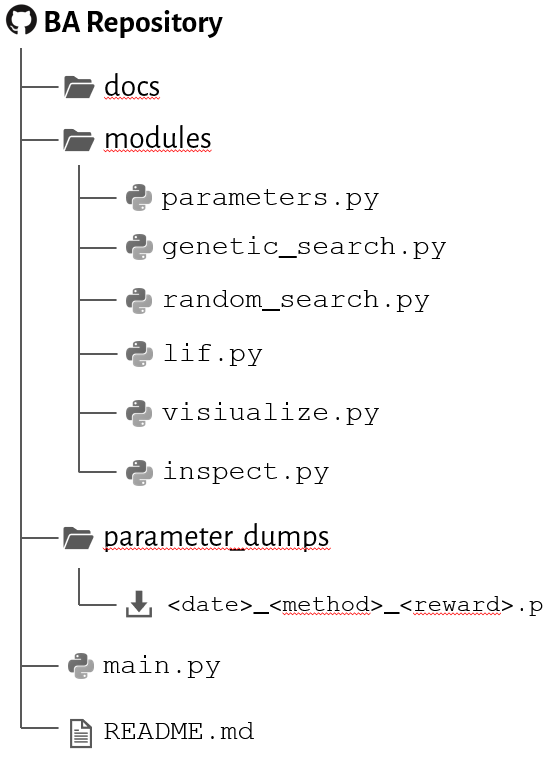
\includegraphics[width=4cm]{figures/python_repo.png}
  \end{minipage}

\end{frame}

% =======================

\begin{frame}
  \frametitle{Ergebnisse}
  \framesubtitle{Statusgespräch am 18. Juli 2018}

  \begin{itemize}
  	\item Review des Programmcodes und Verbesserungsvorschläge:
  	\begin{itemize}
  		\item Verhalten des neuronalen Netzes überprüfen (Verhalten noch unregelmäßig)
  		\item Neue Plots zum inspizieren des Verhalten der Umgebung (bspw. Aktion zu Winkel)
  		\item LIF-Modell: Variaton der Integrationsschrittweite zur besseren Kontrolle der Feuer-Zeiten
  	\end{itemize}
  	\item Neue Such-Algorithmen zur besseren Anwendung des Reinforcement Learning-Ansatzes
  	\item Beginn der kompletten Dokumentation und sukzessives Schreiben der Bachelorarbeit
  \end{itemize}

\end{frame}

% =======================

\begin{frame}
  \frametitle{Sonstiges}
  
  Programmcode und sonstige Informationen auf GitHub - \href{https://github.com/J0nasW/BA}{\ctEmph{J0nasW/BA}}\\
  \vspace{1cm}
  Environment - OpenAI Gym - \href{https://gym.openai.com/envs/CartPole-v0/}{\ctEmph{CartPole-v0}}\\
  \vspace{1cm}
  Programmiersprache: Python 2.7 - Atom Editor\\

\end{frame}

% =======================



\ClosingSlide

\end{document}

%%% Local Variables:
%%% mode: latex
%%% TeX-master: t
%%% End:
